\documentclass[twoside]{book}

% Packages required by doxygen
\usepackage{fixltx2e}
\usepackage{calc}
\usepackage{doxygen}
\usepackage{graphicx}
\usepackage[utf8]{inputenc}
\usepackage{makeidx}
\usepackage{multicol}
\usepackage{multirow}
\PassOptionsToPackage{warn}{textcomp}
\usepackage{textcomp}
\usepackage[nointegrals]{wasysym}
\usepackage[table]{xcolor}

% NLS support packages
\usepackage[italian]{babel}

% Font selection
\usepackage[T1]{fontenc}
\usepackage{mathptmx}
\usepackage[scaled=.90]{helvet}
\usepackage{courier}
\usepackage{amssymb}
\usepackage{sectsty}
\renewcommand{\familydefault}{\sfdefault}
\allsectionsfont{%
  \fontseries{bc}\selectfont%
  \color{darkgray}%
}
\renewcommand{\DoxyLabelFont}{%
  \fontseries{bc}\selectfont%
  \color{darkgray}%
}
\newcommand{\+}{\discretionary{\mbox{\scriptsize$\hookleftarrow$}}{}{}}

% Page & text layout
\usepackage{geometry}
\geometry{%
  a4paper,%
  top=2.5cm,%
  bottom=2.5cm,%
  left=2.5cm,%
  right=2.5cm%
}
\tolerance=750
\hfuzz=15pt
\hbadness=750
\setlength{\emergencystretch}{15pt}
\setlength{\parindent}{0cm}
\setlength{\parskip}{0.2cm}
\makeatletter
\renewcommand{\paragraph}{%
  \@startsection{paragraph}{4}{0ex}{-1.0ex}{1.0ex}{%
    \normalfont\normalsize\bfseries\SS@parafont%
  }%
}
\renewcommand{\subparagraph}{%
  \@startsection{subparagraph}{5}{0ex}{-1.0ex}{1.0ex}{%
    \normalfont\normalsize\bfseries\SS@subparafont%
  }%
}
\makeatother

% Headers & footers
\usepackage{fancyhdr}
\pagestyle{fancyplain}
\fancyhead[LE]{\fancyplain{}{\bfseries\thepage}}
\fancyhead[CE]{\fancyplain{}{}}
\fancyhead[RE]{\fancyplain{}{\bfseries\leftmark}}
\fancyhead[LO]{\fancyplain{}{\bfseries\rightmark}}
\fancyhead[CO]{\fancyplain{}{}}
\fancyhead[RO]{\fancyplain{}{\bfseries\thepage}}
\fancyfoot[LE]{\fancyplain{}{}}
\fancyfoot[CE]{\fancyplain{}{}}
\fancyfoot[RE]{\fancyplain{}{\bfseries\scriptsize Generato Mar 27 Giu 2017 08\+:13\+:30 per Zynq-\/7000 Driver Pack da Doxygen }}
\fancyfoot[LO]{\fancyplain{}{\bfseries\scriptsize Generato Mar 27 Giu 2017 08\+:13\+:30 per Zynq-\/7000 Driver Pack da Doxygen }}
\fancyfoot[CO]{\fancyplain{}{}}
\fancyfoot[RO]{\fancyplain{}{}}
\renewcommand{\footrulewidth}{0.4pt}
\renewcommand{\chaptermark}[1]{%
  \markboth{#1}{}%
}
\renewcommand{\sectionmark}[1]{%
  \markright{\thesection\ #1}%
}

% Indices & bibliography
\usepackage{natbib}
\usepackage[titles]{tocloft}
\setcounter{tocdepth}{3}
\setcounter{secnumdepth}{5}
\makeindex

% Hyperlinks (required, but should be loaded last)
\usepackage{ifpdf}
\ifpdf
  \usepackage[pdftex,pagebackref=true]{hyperref}
\else
  \usepackage[ps2pdf,pagebackref=true]{hyperref}
\fi
\hypersetup{%
  colorlinks=true,%
  linkcolor=blue,%
  citecolor=blue,%
  unicode%
}

% Custom commands
\newcommand{\clearemptydoublepage}{%
  \newpage{\pagestyle{empty}\cleardoublepage}%
}


%===== C O N T E N T S =====

\begin{document}

% Titlepage & ToC
\hypersetup{pageanchor=false,
             bookmarks=true,
             bookmarksnumbered=true,
             pdfencoding=unicode
            }
\pagenumbering{roman}
\begin{titlepage}
\vspace*{7cm}
\begin{center}%
{\Large Zynq-\/7000 Driver Pack \\[1ex]\large 3.\+1 }\\
\vspace*{1cm}
{\large Generato da Doxygen 1.8.8}\\
\vspace*{0.5cm}
{\small Mar 27 Giu 2017 08:13:30}\\
\end{center}
\end{titlepage}
\clearemptydoublepage
\tableofcontents
\clearemptydoublepage
\pagenumbering{arabic}
\hypersetup{pageanchor=true}

%--- Begin generated contents ---
\chapter{Indice dei moduli}
\section{Moduli}
Questo è l'elenco di tutti i moduli\+:\begin{DoxyCompactList}
\item \contentsline{section}{L\+C\+D}{\pageref{group___l_c_d}}{}
\begin{DoxyCompactList}
\item \contentsline{section}{H\+D44780}{\pageref{group___h_d44780}}{}
\end{DoxyCompactList}
\item \contentsline{section}{Zybo}{\pageref{group___zybo}}{}
\begin{DoxyCompactList}
\item \contentsline{section}{Button}{\pageref{group___button}}{}
\item \contentsline{section}{Led}{\pageref{group___led}}{}
\item \contentsline{section}{Switch}{\pageref{group___switch}}{}
\end{DoxyCompactList}
\item \contentsline{section}{G\+P\+I\+O}{\pageref{group___g_p_i_o}}{}
\end{DoxyCompactList}

\chapter{Indice delle strutture dati}
\section{Strutture dati}
Queste sono le strutture dati con una loro breve descrizione\+:\begin{DoxyCompactList}
\item\contentsline{section}{\hyperlink{struct_g_p_i_o__t}{G\+P\+I\+O\+\_\+t} \\*Struttura che astrae un device G\+P\+I\+O }{\pageref{struct_g_p_i_o__t}}{}
\item\contentsline{section}{\hyperlink{struct_h_d44780___l_c_d__t}{H\+D44780\+\_\+\+L\+C\+D\+\_\+t} \\*Struttura opaca che astrae un device Display L\+C\+D con cntroller Hitachi H\+D44780, o compatibile. Un oggetto di tipo \hyperlink{struct_h_d44780___l_c_d__t}{H\+D44780\+\_\+\+L\+C\+D\+\_\+t} rappresenta un device lcd H\+D44780. Il modulo e' pensato per permettere la gestione di piu' display da parte dello stesso processore, agendo su oggetti \hyperlink{struct_h_d44780___l_c_d__t}{H\+D44780\+\_\+\+L\+C\+D\+\_\+t} diversi. Il modulo permette di utilizzare sia l'interfacciamento ad otto bit che quello a quattro bit, inizializzando il device opportunamente, attraverso l'uso delle funzioni H\+D44780\+\_\+\+Init8 e\+H\+D44780\+\_\+\+Init4. Il modulo fornisce anche semplici funzioni per la stampa di un carattere o di una stringa null-\/terminated di caratteri. Si veda la documentazione delle funzioni H\+D44780\+\_\+\+Printc e H\+D44780\+\_\+\+Print. Inoltre sono presenti diverse funzioni di utilita' generica, come quelle per la pulizia del display, per lo spostamento del cursore di un posto in avanti o indietro, alla riga in basso o in alto }{\pageref{struct_h_d44780___l_c_d__t}}{}
\item\contentsline{section}{\hyperlink{struct_zybo_button__t}{Zybo\+Button\+\_\+t} \\*Struttura opaca che astrae l'insieme dei button presenti sulla board Digilent Zybo; }{\pageref{struct_zybo_button__t}}{}
\item\contentsline{section}{\hyperlink{struct_zybo_led__t}{Zybo\+Led\+\_\+t} \\*Struttura opaca che astrae l'insieme dei Led presenti sulla board Digilent Zybo; }{\pageref{struct_zybo_led__t}}{}
\item\contentsline{section}{\hyperlink{struct_zybo_switch__t}{Zybo\+Switch\+\_\+t} \\*Struttura opaca che astrae l'insieme degli switch presenti sulla board Digilent Zybo; }{\pageref{struct_zybo_switch__t}}{}
\end{DoxyCompactList}

\chapter{Indice dei file}
\section{Elenco dei file}
Questo è un elenco di tutti i file con una loro breve descrizione\+:\begin{DoxyCompactList}
\item\contentsline{section}{G\+P\+I\+O/\hyperlink{my_g_p_i_o_8c}{my\+G\+P\+I\+O.\+c} }{\pageref{my_g_p_i_o_8c}}{}
\item\contentsline{section}{G\+P\+I\+O/\hyperlink{my_g_p_i_o_8h}{my\+G\+P\+I\+O.\+h} }{\pageref{my_g_p_i_o_8h}}{}
\item\contentsline{section}{Lcd/\hyperlink{hd44780_8c}{hd44780.\+c} }{\pageref{hd44780_8c}}{}
\item\contentsline{section}{Lcd/\hyperlink{hd44780_8h}{hd44780.\+h} }{\pageref{hd44780_8h}}{}
\item\contentsline{section}{Zybo/\hyperlink{_zybo_8h}{Zybo.\+h} }{\pageref{_zybo_8h}}{}
\item\contentsline{section}{Zybo/\hyperlink{_zybo_button_8c}{Zybo\+Button.\+c} }{\pageref{_zybo_button_8c}}{}
\item\contentsline{section}{Zybo/\hyperlink{_zybo_button_8h}{Zybo\+Button.\+h} }{\pageref{_zybo_button_8h}}{}
\item\contentsline{section}{Zybo/\hyperlink{_zybo_led_8c}{Zybo\+Led.\+c} }{\pageref{_zybo_led_8c}}{}
\item\contentsline{section}{Zybo/\hyperlink{_zybo_led_8h}{Zybo\+Led.\+h} }{\pageref{_zybo_led_8h}}{}
\item\contentsline{section}{Zybo/\hyperlink{_zybo_switch_8c}{Zybo\+Switch.\+c} }{\pageref{_zybo_switch_8c}}{}
\item\contentsline{section}{Zybo/\hyperlink{_zybo_switch_8h}{Zybo\+Switch.\+h} }{\pageref{_zybo_switch_8h}}{}
\end{DoxyCompactList}

\chapter{Documentazione dei moduli}
\hypertarget{group__bare-metal}{\section{Bare-\/metal}
\label{group__bare-metal}\index{Bare-\/metal@{Bare-\/metal}}
}


device-\/driver O\+O-\/like bare-\/metal per device my\+G\+P\+I\+O  


Diagramma di collaborazione per Bare-\/metal\+:\nopagebreak
\begin{figure}[H]
\begin{center}
\leavevmode
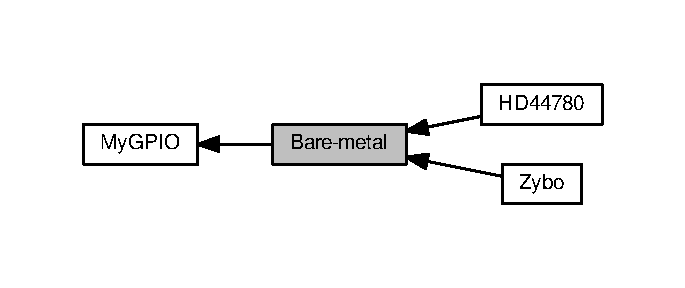
\includegraphics[width=329pt]{group__bare-metal}
\end{center}
\end{figure}
\subsection*{Moduli}
\begin{DoxyCompactItemize}
\item 
\hyperlink{group___h_d44780}{H\+D44780}
\begin{DoxyCompactList}\small\item\em driver per display Hitachi hd44780 basato su driver my\+G\+P\+I\+O bare-\/metal \end{DoxyCompactList}\item 
\hyperlink{group___zybo}{Zybo}
\end{DoxyCompactItemize}
\subsection*{Strutture dati}
\begin{DoxyCompactItemize}
\item 
struct \hyperlink{structmy_g_p_i_o__t}{my\+G\+P\+I\+O\+\_\+t}
\begin{DoxyCompactList}\small\item\em Struttura che astrae un device my\+G\+P\+I\+O. \end{DoxyCompactList}\end{DoxyCompactItemize}
\subsection*{Definizioni}
\begin{DoxyCompactItemize}
\item 
\#define \hyperlink{group__bare-metal_ga81a662103d6ed053978c0a9b4c273065}{my\+G\+P\+I\+O\+\_\+\+M\+O\+D\+E\+\_\+\+O\+F\+F\+S\+E\+T}~0x00\+U
\begin{DoxyCompactList}\small\item\em Offset, rispetto all'indirizzo base, del registro \char`\"{}mode\char`\"{} per il device my\+G\+P\+I\+O. \end{DoxyCompactList}\item 
\#define \hyperlink{group__bare-metal_ga2e45778b6ca9ce6f5768b3f7a4557ce1}{my\+G\+P\+I\+O\+\_\+\+W\+R\+I\+T\+E\+\_\+\+O\+F\+F\+S\+E\+T}~0x04\+U
\begin{DoxyCompactList}\small\item\em Offset, rispetto all'indirizzo base, del registro \char`\"{}write\char`\"{} per il device my\+G\+P\+I\+O. \end{DoxyCompactList}\item 
\#define \hyperlink{group__bare-metal_ga584d2dfece76e5762030d918d80592cc}{my\+G\+P\+I\+O\+\_\+\+R\+E\+A\+D\+\_\+\+O\+F\+F\+S\+E\+T}~0x08\+U
\begin{DoxyCompactList}\small\item\em Offset, rispetto all'indirizzo base, del registro \char`\"{}read\char`\"{} per il device my\+G\+P\+I\+O. \end{DoxyCompactList}\item 
\#define \hyperlink{group__bare-metal_gad251e4d87d464525d4a2858977468994}{my\+G\+P\+I\+O\+\_\+\+G\+I\+E\+S\+\_\+\+O\+F\+F\+S\+E\+T}~0x0\+C\+U
\begin{DoxyCompactList}\small\item\em Offset, rispetto all'indirizzo base, del registro \char`\"{}gies\char`\"{} per il device my\+G\+P\+I\+O. \end{DoxyCompactList}\item 
\#define \hyperlink{group__bare-metal_gaece3c1c9f504249d6b8ab060d8bb2738}{my\+G\+P\+I\+O\+\_\+\+P\+I\+E\+\_\+\+O\+F\+F\+S\+E\+T}~0x10\+U
\begin{DoxyCompactList}\small\item\em Offset, rispetto all'indirizzo base, del registro \char`\"{}pie\char`\"{} per il device my\+G\+P\+I\+O. \end{DoxyCompactList}\item 
\#define \hyperlink{group__bare-metal_ga31a7c2a9de5c63576f2f5aa061b936c5}{my\+G\+P\+I\+O\+\_\+\+I\+R\+Q\+\_\+\+O\+F\+F\+S\+E\+T}~0x14\+U
\begin{DoxyCompactList}\small\item\em Offset, rispetto all'indirizzo base, del registro \char`\"{}irq\char`\"{} per il device my\+G\+P\+I\+O. \end{DoxyCompactList}\item 
\#define \hyperlink{group__bare-metal_gadfca866ac50c2dae09c3c46ad80670fc}{my\+G\+P\+I\+O\+\_\+\+I\+A\+C\+K\+\_\+\+O\+F\+F\+S\+E\+T}~0x18\+U
\begin{DoxyCompactList}\small\item\em Offset, rispetto all'indirizzo base, del registro \char`\"{}iack\char`\"{} per il device my\+G\+P\+I\+O. \end{DoxyCompactList}\item 
\#define \hyperlink{group__bare-metal_gabbe2491a3b71c292521025b7b382b971}{my\+G\+P\+I\+O\+\_\+pin}(i)~((uint32\+\_\+t)(1$<$$<$(i)))
\begin{DoxyCompactList}\small\item\em Metodo alternativo per la specifica di uno dei pin di un device my\+G\+P\+I\+O. \end{DoxyCompactList}\end{DoxyCompactItemize}
\subsection*{Tipi enumerati (enum)}
\begin{DoxyCompactItemize}
\item 
enum \hyperlink{group__bare-metal_ga402a0d20afc0cb7c25554b8b023f4253}{my\+G\+P\+I\+O\+\_\+mask} \{ \\*
\hyperlink{group__bare-metal_gga402a0d20afc0cb7c25554b8b023f4253a6db6fa7be955ae379f543d96122e23a9}{my\+G\+P\+I\+O\+\_\+pin0} = 0x1\+U, 
\hyperlink{group__bare-metal_gga402a0d20afc0cb7c25554b8b023f4253a1de6bdcc01efca2c39f584f5a20293be}{my\+G\+P\+I\+O\+\_\+pin1} = 0x2\+U, 
\hyperlink{group__bare-metal_gga402a0d20afc0cb7c25554b8b023f4253a1fb3f52d920ac8ba17b74dd73c27d783}{my\+G\+P\+I\+O\+\_\+pin2} = 0x4\+U, 
\hyperlink{group__bare-metal_gga402a0d20afc0cb7c25554b8b023f4253a4514d64390392b626aa4dbfaac8dc1e5}{my\+G\+P\+I\+O\+\_\+pin3} = 0x8\+U, 
\\*
\hyperlink{group__bare-metal_gga402a0d20afc0cb7c25554b8b023f4253a0a446f53dee6f6f4ccb9a1d1f947b637}{my\+G\+P\+I\+O\+\_\+pin4} = 0x10\+U, 
\hyperlink{group__bare-metal_gga402a0d20afc0cb7c25554b8b023f4253a04a111036a27e9b97f0950f6d37b04d2}{my\+G\+P\+I\+O\+\_\+pin5} = 0x20\+U, 
\hyperlink{group__bare-metal_gga402a0d20afc0cb7c25554b8b023f4253a39a529f8c0a4f302029f54daa815471b}{my\+G\+P\+I\+O\+\_\+pin6} = 0x40\+U, 
\hyperlink{group__bare-metal_gga402a0d20afc0cb7c25554b8b023f4253af4e88b077442e4c0f459e1e4aa60626b}{my\+G\+P\+I\+O\+\_\+pin7} = 0x80\+U, 
\\*
\hyperlink{group__bare-metal_gga402a0d20afc0cb7c25554b8b023f4253a615159bcf4e347dc2b60f2545fae5f9e}{my\+G\+P\+I\+O\+\_\+pin8} = 0x100\+U, 
\hyperlink{group__bare-metal_gga402a0d20afc0cb7c25554b8b023f4253a8d721236fb936126a08c12b87696f6e9}{my\+G\+P\+I\+O\+\_\+pin9} = 0x200\+U, 
\hyperlink{group__bare-metal_gga402a0d20afc0cb7c25554b8b023f4253ae3067b7b3b1a2e171ecd74b6abd48341}{my\+G\+P\+I\+O\+\_\+pin10} = 0x400\+U, 
\hyperlink{group__bare-metal_gga402a0d20afc0cb7c25554b8b023f4253ae5c2e65508bfd452100d9da331d6220a}{my\+G\+P\+I\+O\+\_\+pin11} = 0x800\+U, 
\\*
\hyperlink{group__bare-metal_gga402a0d20afc0cb7c25554b8b023f4253afa75e3c1c019048c8553cb733c5137b5}{my\+G\+P\+I\+O\+\_\+pin12} = 0x1000\+U, 
\hyperlink{group__bare-metal_gga402a0d20afc0cb7c25554b8b023f4253a243381a796f0936a576f184dd115b37c}{my\+G\+P\+I\+O\+\_\+pin13} = 0x2000\+U, 
\hyperlink{group__bare-metal_gga402a0d20afc0cb7c25554b8b023f4253aed4915d6b3eab49cc1ba971b9f439fdd}{my\+G\+P\+I\+O\+\_\+pin14} = 0x4000\+U, 
\hyperlink{group__bare-metal_gga402a0d20afc0cb7c25554b8b023f4253a46c427ea97182a77e8c975d3429a64ee}{my\+G\+P\+I\+O\+\_\+pin15} = 0x8000\+U, 
\\*
\hyperlink{group__bare-metal_gga402a0d20afc0cb7c25554b8b023f4253a5a27c4d87207b2eba865876854f1ba67}{my\+G\+P\+I\+O\+\_\+pin16} = 0x10000\+U, 
\hyperlink{group__bare-metal_gga402a0d20afc0cb7c25554b8b023f4253ab0541af31059bdc8dca44d5dafa7e779}{my\+G\+P\+I\+O\+\_\+pin17} = 0x20000\+U, 
\hyperlink{group__bare-metal_gga402a0d20afc0cb7c25554b8b023f4253a7a51a492e3cb580581a2c8eb439edd99}{my\+G\+P\+I\+O\+\_\+pin18} = 0x40000\+U, 
\hyperlink{group__bare-metal_gga402a0d20afc0cb7c25554b8b023f4253a9118ae2775e93bd4522660e81a2d5309}{my\+G\+P\+I\+O\+\_\+pin19} = 0x80000\+U, 
\\*
\hyperlink{group__bare-metal_gga402a0d20afc0cb7c25554b8b023f4253a7940782a16f88dbbb3a4037c2bef1711}{my\+G\+P\+I\+O\+\_\+pin20} = 0x100000\+U, 
\hyperlink{group__bare-metal_gga402a0d20afc0cb7c25554b8b023f4253a1da616a8cf4396927db1e5a336fb6dc5}{my\+G\+P\+I\+O\+\_\+pin21} = 0x200000\+U, 
\hyperlink{group__bare-metal_gga402a0d20afc0cb7c25554b8b023f4253acf80113da8d789f7da9f9edc4ab6003c}{my\+G\+P\+I\+O\+\_\+pin22} = 0x400000\+U, 
\hyperlink{group__bare-metal_gga402a0d20afc0cb7c25554b8b023f4253ad64e03b703608de173ab5950b5121830}{my\+G\+P\+I\+O\+\_\+pin23} = 0x800000\+U, 
\\*
\hyperlink{group__bare-metal_gga402a0d20afc0cb7c25554b8b023f4253a5bb93f546327123f81b06ed0dfcdf110}{my\+G\+P\+I\+O\+\_\+pin24} = 0x1000000\+U, 
\hyperlink{group__bare-metal_gga402a0d20afc0cb7c25554b8b023f4253a0b27a7e78aff5836f33085f3b4539f56}{my\+G\+P\+I\+O\+\_\+pin25} = 0x2000000\+U, 
\hyperlink{group__bare-metal_gga402a0d20afc0cb7c25554b8b023f4253aaa07c24140250dcbc695206793efa8af}{my\+G\+P\+I\+O\+\_\+pin26} = 0x4000000\+U, 
\hyperlink{group__bare-metal_gga402a0d20afc0cb7c25554b8b023f4253a1dd5e99eba6237aeb30b2194c553c37f}{my\+G\+P\+I\+O\+\_\+pin27} = 0x8000000\+U, 
\\*
\hyperlink{group__bare-metal_gga402a0d20afc0cb7c25554b8b023f4253a2076590efec8bcf9ef3285798753e632}{my\+G\+P\+I\+O\+\_\+pin28} = 0x10000000\+U, 
\hyperlink{group__bare-metal_gga402a0d20afc0cb7c25554b8b023f4253abfe9540fa3946a35e20f7f68cb1b8084}{my\+G\+P\+I\+O\+\_\+pin29} = 0x20000000\+U, 
\hyperlink{group__bare-metal_gga402a0d20afc0cb7c25554b8b023f4253a59993a30c537c116eddb42d10778f4f8}{my\+G\+P\+I\+O\+\_\+pin30} = 0x40000000\+U, 
\hyperlink{group__bare-metal_gga402a0d20afc0cb7c25554b8b023f4253a9a55b7c245bd9aad750b7891d27e9225}{my\+G\+P\+I\+O\+\_\+pin31} = 0x80000000\+U, 
\\*
\hyperlink{group__bare-metal_gga402a0d20afc0cb7c25554b8b023f4253a0347b1742eef6b2575a7d409c7fb5c3d}{my\+G\+P\+I\+O\+\_\+byte0} = 0x000000ff\+U, 
\hyperlink{group__bare-metal_gga402a0d20afc0cb7c25554b8b023f4253ae5aec65fa20f554b893e419fc2755fd0}{my\+G\+P\+I\+O\+\_\+byte1} = 0x0000ff00\+U, 
\hyperlink{group__bare-metal_gga402a0d20afc0cb7c25554b8b023f4253af4892f7db28c64a7cf2a7236c88b742b}{my\+G\+P\+I\+O\+\_\+byte2} = 0x00ff0000\+U, 
\hyperlink{group__bare-metal_gga402a0d20afc0cb7c25554b8b023f4253a1ceefb9d65397352e986c573984d0129}{my\+G\+P\+I\+O\+\_\+byte3} = 0xff000000\+U
 \}
\begin{DoxyCompactList}\small\item\em Maschere di selezione dei pin di un device my\+G\+P\+I\+O. \end{DoxyCompactList}\item 
enum \hyperlink{group__bare-metal_ga76b849f0e0c05e7f9161bdb33396f2b1}{my\+G\+P\+I\+O\+\_\+mode} \{ \hyperlink{group__bare-metal_gga76b849f0e0c05e7f9161bdb33396f2b1a1e6dc78e7641e878cadc842d39605d5d}{my\+G\+P\+I\+O\+\_\+read}, 
\hyperlink{group__bare-metal_gga76b849f0e0c05e7f9161bdb33396f2b1a2d66976280eb7595a42c631683bdfad6}{my\+G\+P\+I\+O\+\_\+write}
 \}
\begin{DoxyCompactList}\small\item\em my\+G\+P\+I\+O\+\_\+mode, modalità di funzionamento (lettura/scrittura) di un device my\+G\+P\+I\+O \end{DoxyCompactList}\item 
enum \hyperlink{group__bare-metal_gaf634fe4a0e1eab8da5000b72d6ad362b}{my\+G\+P\+I\+O\+\_\+value} \{ \hyperlink{group__bare-metal_ggaf634fe4a0e1eab8da5000b72d6ad362ba98cde80dbda025bd1ae7231c76b55674}{my\+G\+P\+I\+O\+\_\+reset}, 
\hyperlink{group__bare-metal_ggaf634fe4a0e1eab8da5000b72d6ad362ba10d296f3711d01189cc6c2d87f7c9149}{my\+G\+P\+I\+O\+\_\+set}
 \}
\begin{DoxyCompactList}\small\item\em my\+G\+P\+I\+O\+\_\+value, valore di un my\+G\+P\+I\+O \end{DoxyCompactList}\end{DoxyCompactItemize}
\subsection*{Funzioni}
\begin{DoxyCompactItemize}
\item 
void \hyperlink{group__bare-metal_ga588201358d1633c53535b288c9198531}{my\+G\+P\+I\+O\+\_\+\+Init} (\hyperlink{structmy_g_p_i_o__t}{my\+G\+P\+I\+O\+\_\+t} $\ast$gpio, uint32\+\_\+t base\+\_\+address)
\begin{DoxyCompactList}\small\item\em Inizializza un device my\+G\+P\+I\+O. \end{DoxyCompactList}\item 
void \hyperlink{group__bare-metal_ga43e82eb0febd452635a438fbd9cb853b}{my\+G\+P\+I\+O\+\_\+\+Set\+Mode} (\hyperlink{structmy_g_p_i_o__t}{my\+G\+P\+I\+O\+\_\+t} $\ast$gpio, \hyperlink{group__bare-metal_ga402a0d20afc0cb7c25554b8b023f4253}{my\+G\+P\+I\+O\+\_\+mask} mask, \hyperlink{group__bare-metal_ga76b849f0e0c05e7f9161bdb33396f2b1}{my\+G\+P\+I\+O\+\_\+mode} mode)
\begin{DoxyCompactList}\small\item\em Permette di settare la modalità lettura/scrittura dei pin di un device my\+G\+P\+I\+O;. \end{DoxyCompactList}\item 
void \hyperlink{group__bare-metal_ga9d9ce9d2db7d77a588da4a3749f2f24d}{my\+G\+P\+I\+O\+\_\+\+Set\+Value} (\hyperlink{structmy_g_p_i_o__t}{my\+G\+P\+I\+O\+\_\+t} $\ast$gpio, \hyperlink{group__bare-metal_ga402a0d20afc0cb7c25554b8b023f4253}{my\+G\+P\+I\+O\+\_\+mask} mask, \hyperlink{group__bare-metal_gaf634fe4a0e1eab8da5000b72d6ad362b}{my\+G\+P\+I\+O\+\_\+value} value)
\begin{DoxyCompactList}\small\item\em Permette di settare il valore dei pin di un device my\+G\+P\+I\+O, se configurati come output. \end{DoxyCompactList}\item 
void \hyperlink{group__bare-metal_ga449b2af7cc20d24e6f6e017cf792ce03}{my\+G\+P\+I\+O\+\_\+\+Toggle} (\hyperlink{structmy_g_p_i_o__t}{my\+G\+P\+I\+O\+\_\+t} $\ast$gpio, \hyperlink{group__bare-metal_ga402a0d20afc0cb7c25554b8b023f4253}{my\+G\+P\+I\+O\+\_\+mask} mask)
\begin{DoxyCompactList}\small\item\em Permette di invertire il valore dei pin di un device my\+G\+P\+I\+O, se configurati come output. \end{DoxyCompactList}\item 
\hyperlink{group__bare-metal_gaf634fe4a0e1eab8da5000b72d6ad362b}{my\+G\+P\+I\+O\+\_\+value} \hyperlink{group__bare-metal_ga2a20e519816733b90204b975edc4e212}{my\+G\+P\+I\+O\+\_\+\+Get\+Value} (\hyperlink{structmy_g_p_i_o__t}{my\+G\+P\+I\+O\+\_\+t} $\ast$gpio, \hyperlink{group__bare-metal_ga402a0d20afc0cb7c25554b8b023f4253}{my\+G\+P\+I\+O\+\_\+mask} mask)
\begin{DoxyCompactList}\small\item\em Permette di leggere il valore dei pin di un device my\+G\+P\+I\+O;. \end{DoxyCompactList}\item 
\hyperlink{group__bare-metal_ga402a0d20afc0cb7c25554b8b023f4253}{my\+G\+P\+I\+O\+\_\+mask} \hyperlink{group__bare-metal_gac35776cd6652f7b932a132f3f6959a11}{my\+G\+P\+I\+O\+\_\+\+Get\+Read} (\hyperlink{structmy_g_p_i_o__t}{my\+G\+P\+I\+O\+\_\+t} $\ast$gpio)
\begin{DoxyCompactList}\small\item\em Restituisce la maschera dei pin settati di un device my\+G\+P\+I\+O. \end{DoxyCompactList}\item 
void \hyperlink{group__bare-metal_gada93ef6a9818e634f0a233ce14582216}{my\+G\+P\+I\+O\+\_\+\+Global\+Interrupt\+Enable} (\hyperlink{structmy_g_p_i_o__t}{my\+G\+P\+I\+O\+\_\+t} $\ast$gpio)
\begin{DoxyCompactList}\small\item\em Abilita gli interrupt globali;. \end{DoxyCompactList}\item 
void \hyperlink{group__bare-metal_gaacca2871ac57a166e62bf431a2da7548}{my\+G\+P\+I\+O\+\_\+\+Global\+Interrupt\+Disable} (\hyperlink{structmy_g_p_i_o__t}{my\+G\+P\+I\+O\+\_\+t} $\ast$gpio)
\begin{DoxyCompactList}\small\item\em Disabilita gli interrupt globali;. \end{DoxyCompactList}\item 
\hyperlink{group__bare-metal_gaf634fe4a0e1eab8da5000b72d6ad362b}{my\+G\+P\+I\+O\+\_\+value} \hyperlink{group__bare-metal_ga0a753db3d02ad08014e4b7304e0f1829}{my\+G\+P\+I\+O\+\_\+\+Is\+Global\+Interrupt\+Enabled} (\hyperlink{structmy_g_p_i_o__t}{my\+G\+P\+I\+O\+\_\+t} $\ast$gpio)
\begin{DoxyCompactList}\small\item\em Consente di verificare se gli interrupt globali siano abilitati. \end{DoxyCompactList}\item 
\hyperlink{group__bare-metal_gaf634fe4a0e1eab8da5000b72d6ad362b}{my\+G\+P\+I\+O\+\_\+value} \hyperlink{group__bare-metal_ga386cea84aca8c6bb731b4b46fcbf9199}{my\+G\+P\+I\+O\+\_\+\+Pending\+Interrupt} (\hyperlink{structmy_g_p_i_o__t}{my\+G\+P\+I\+O\+\_\+t} $\ast$gpio)
\begin{DoxyCompactList}\small\item\em Consente di verificare se esistano interrupt non ancora serviti. \end{DoxyCompactList}\item 
void \hyperlink{group__bare-metal_ga116e3a1077a317e9e42ded6dd4df64af}{my\+G\+P\+I\+O\+\_\+\+Pin\+Interrupt\+Enable} (\hyperlink{structmy_g_p_i_o__t}{my\+G\+P\+I\+O\+\_\+t} $\ast$gpio, \hyperlink{group__bare-metal_ga402a0d20afc0cb7c25554b8b023f4253}{my\+G\+P\+I\+O\+\_\+mask} mask)
\begin{DoxyCompactList}\small\item\em Abilita gli interrupt per i singoli pin del device. \end{DoxyCompactList}\item 
void \hyperlink{group__bare-metal_ga37d3df33ac50387d6f2e1fb5e2b13e49}{my\+G\+P\+I\+O\+\_\+\+Pin\+Interrupt\+Disable} (\hyperlink{structmy_g_p_i_o__t}{my\+G\+P\+I\+O\+\_\+t} $\ast$gpio, \hyperlink{group__bare-metal_ga402a0d20afc0cb7c25554b8b023f4253}{my\+G\+P\+I\+O\+\_\+mask} mask)
\begin{DoxyCompactList}\small\item\em Disabilita gli interrupt per i singoli pin del device. \end{DoxyCompactList}\item 
\hyperlink{group__bare-metal_ga402a0d20afc0cb7c25554b8b023f4253}{my\+G\+P\+I\+O\+\_\+mask} \hyperlink{group__bare-metal_ga80ef1cf3e9bd8bfd4d849a0f3b8e7b2c}{my\+G\+P\+I\+O\+\_\+\+Enabled\+Pin\+Interrupt} (\hyperlink{structmy_g_p_i_o__t}{my\+G\+P\+I\+O\+\_\+t} $\ast$gpio)
\begin{DoxyCompactList}\small\item\em Consente di ottenere una maschera che indichi quali pin abbiano interrupt abilitati. \end{DoxyCompactList}\item 
\hyperlink{group__bare-metal_ga402a0d20afc0cb7c25554b8b023f4253}{my\+G\+P\+I\+O\+\_\+mask} \hyperlink{group__bare-metal_ga6115bde39f860d4e76e7d8f421ce222c}{my\+G\+P\+I\+O\+\_\+\+Pending\+Pin\+Interrupt} (\hyperlink{structmy_g_p_i_o__t}{my\+G\+P\+I\+O\+\_\+t} $\ast$gpio)
\begin{DoxyCompactList}\small\item\em Consente di ottenere una maschera che indichi quali interrupt non siano stati ancora serviti;. \end{DoxyCompactList}\item 
void \hyperlink{group__bare-metal_gab6ad3dda867515825890c97dbf6f55db}{my\+G\+P\+I\+O\+\_\+\+Pin\+Interrupt\+Ack} (\hyperlink{structmy_g_p_i_o__t}{my\+G\+P\+I\+O\+\_\+t} $\ast$gpio, \hyperlink{group__bare-metal_ga402a0d20afc0cb7c25554b8b023f4253}{my\+G\+P\+I\+O\+\_\+mask} mask)
\begin{DoxyCompactList}\small\item\em Invia al device notifica di servizio di un interrupt;. \end{DoxyCompactList}\end{DoxyCompactItemize}


\subsection{Descrizione dettagliata}
device-\/driver O\+O-\/like bare-\/metal per device my\+G\+P\+I\+O 



\subsection{Documentazione delle definizioni}
\hypertarget{group__bare-metal_gad251e4d87d464525d4a2858977468994}{\index{Bare-\/metal@{Bare-\/metal}!my\+G\+P\+I\+O\+\_\+\+G\+I\+E\+S\+\_\+\+O\+F\+F\+S\+E\+T@{my\+G\+P\+I\+O\+\_\+\+G\+I\+E\+S\+\_\+\+O\+F\+F\+S\+E\+T}}
\index{my\+G\+P\+I\+O\+\_\+\+G\+I\+E\+S\+\_\+\+O\+F\+F\+S\+E\+T@{my\+G\+P\+I\+O\+\_\+\+G\+I\+E\+S\+\_\+\+O\+F\+F\+S\+E\+T}!Bare-\/metal@{Bare-\/metal}}
\subsubsection[{my\+G\+P\+I\+O\+\_\+\+G\+I\+E\+S\+\_\+\+O\+F\+F\+S\+E\+T}]{\setlength{\rightskip}{0pt plus 5cm}\#define my\+G\+P\+I\+O\+\_\+\+G\+I\+E\+S\+\_\+\+O\+F\+F\+S\+E\+T~0x0\+C\+U}}\label{group__bare-metal_gad251e4d87d464525d4a2858977468994}


Offset, rispetto all'indirizzo base, del registro \char`\"{}gies\char`\"{} per il device my\+G\+P\+I\+O. 

\hypertarget{group__bare-metal_gadfca866ac50c2dae09c3c46ad80670fc}{\index{Bare-\/metal@{Bare-\/metal}!my\+G\+P\+I\+O\+\_\+\+I\+A\+C\+K\+\_\+\+O\+F\+F\+S\+E\+T@{my\+G\+P\+I\+O\+\_\+\+I\+A\+C\+K\+\_\+\+O\+F\+F\+S\+E\+T}}
\index{my\+G\+P\+I\+O\+\_\+\+I\+A\+C\+K\+\_\+\+O\+F\+F\+S\+E\+T@{my\+G\+P\+I\+O\+\_\+\+I\+A\+C\+K\+\_\+\+O\+F\+F\+S\+E\+T}!Bare-\/metal@{Bare-\/metal}}
\subsubsection[{my\+G\+P\+I\+O\+\_\+\+I\+A\+C\+K\+\_\+\+O\+F\+F\+S\+E\+T}]{\setlength{\rightskip}{0pt plus 5cm}\#define my\+G\+P\+I\+O\+\_\+\+I\+A\+C\+K\+\_\+\+O\+F\+F\+S\+E\+T~0x18\+U}}\label{group__bare-metal_gadfca866ac50c2dae09c3c46ad80670fc}


Offset, rispetto all'indirizzo base, del registro \char`\"{}iack\char`\"{} per il device my\+G\+P\+I\+O. 

\hypertarget{group__bare-metal_ga31a7c2a9de5c63576f2f5aa061b936c5}{\index{Bare-\/metal@{Bare-\/metal}!my\+G\+P\+I\+O\+\_\+\+I\+R\+Q\+\_\+\+O\+F\+F\+S\+E\+T@{my\+G\+P\+I\+O\+\_\+\+I\+R\+Q\+\_\+\+O\+F\+F\+S\+E\+T}}
\index{my\+G\+P\+I\+O\+\_\+\+I\+R\+Q\+\_\+\+O\+F\+F\+S\+E\+T@{my\+G\+P\+I\+O\+\_\+\+I\+R\+Q\+\_\+\+O\+F\+F\+S\+E\+T}!Bare-\/metal@{Bare-\/metal}}
\subsubsection[{my\+G\+P\+I\+O\+\_\+\+I\+R\+Q\+\_\+\+O\+F\+F\+S\+E\+T}]{\setlength{\rightskip}{0pt plus 5cm}\#define my\+G\+P\+I\+O\+\_\+\+I\+R\+Q\+\_\+\+O\+F\+F\+S\+E\+T~0x14\+U}}\label{group__bare-metal_ga31a7c2a9de5c63576f2f5aa061b936c5}


Offset, rispetto all'indirizzo base, del registro \char`\"{}irq\char`\"{} per il device my\+G\+P\+I\+O. 

\hypertarget{group__bare-metal_ga81a662103d6ed053978c0a9b4c273065}{\index{Bare-\/metal@{Bare-\/metal}!my\+G\+P\+I\+O\+\_\+\+M\+O\+D\+E\+\_\+\+O\+F\+F\+S\+E\+T@{my\+G\+P\+I\+O\+\_\+\+M\+O\+D\+E\+\_\+\+O\+F\+F\+S\+E\+T}}
\index{my\+G\+P\+I\+O\+\_\+\+M\+O\+D\+E\+\_\+\+O\+F\+F\+S\+E\+T@{my\+G\+P\+I\+O\+\_\+\+M\+O\+D\+E\+\_\+\+O\+F\+F\+S\+E\+T}!Bare-\/metal@{Bare-\/metal}}
\subsubsection[{my\+G\+P\+I\+O\+\_\+\+M\+O\+D\+E\+\_\+\+O\+F\+F\+S\+E\+T}]{\setlength{\rightskip}{0pt plus 5cm}\#define my\+G\+P\+I\+O\+\_\+\+M\+O\+D\+E\+\_\+\+O\+F\+F\+S\+E\+T~0x00\+U}}\label{group__bare-metal_ga81a662103d6ed053978c0a9b4c273065}


Offset, rispetto all'indirizzo base, del registro \char`\"{}mode\char`\"{} per il device my\+G\+P\+I\+O. 

\hypertarget{group__bare-metal_gaece3c1c9f504249d6b8ab060d8bb2738}{\index{Bare-\/metal@{Bare-\/metal}!my\+G\+P\+I\+O\+\_\+\+P\+I\+E\+\_\+\+O\+F\+F\+S\+E\+T@{my\+G\+P\+I\+O\+\_\+\+P\+I\+E\+\_\+\+O\+F\+F\+S\+E\+T}}
\index{my\+G\+P\+I\+O\+\_\+\+P\+I\+E\+\_\+\+O\+F\+F\+S\+E\+T@{my\+G\+P\+I\+O\+\_\+\+P\+I\+E\+\_\+\+O\+F\+F\+S\+E\+T}!Bare-\/metal@{Bare-\/metal}}
\subsubsection[{my\+G\+P\+I\+O\+\_\+\+P\+I\+E\+\_\+\+O\+F\+F\+S\+E\+T}]{\setlength{\rightskip}{0pt plus 5cm}\#define my\+G\+P\+I\+O\+\_\+\+P\+I\+E\+\_\+\+O\+F\+F\+S\+E\+T~0x10\+U}}\label{group__bare-metal_gaece3c1c9f504249d6b8ab060d8bb2738}


Offset, rispetto all'indirizzo base, del registro \char`\"{}pie\char`\"{} per il device my\+G\+P\+I\+O. 

\hypertarget{group__bare-metal_gabbe2491a3b71c292521025b7b382b971}{\index{Bare-\/metal@{Bare-\/metal}!my\+G\+P\+I\+O\+\_\+pin@{my\+G\+P\+I\+O\+\_\+pin}}
\index{my\+G\+P\+I\+O\+\_\+pin@{my\+G\+P\+I\+O\+\_\+pin}!Bare-\/metal@{Bare-\/metal}}
\subsubsection[{my\+G\+P\+I\+O\+\_\+pin}]{\setlength{\rightskip}{0pt plus 5cm}\#define my\+G\+P\+I\+O\+\_\+pin(
\begin{DoxyParamCaption}
\item[{}]{i}
\end{DoxyParamCaption}
)~((uint32\+\_\+t)(1$<$$<$(i)))}}\label{group__bare-metal_gabbe2491a3b71c292521025b7b382b971}


Metodo alternativo per la specifica di uno dei pin di un device my\+G\+P\+I\+O. 


\begin{DoxyParams}[1]{Parametri}
\mbox{\tt in}  & {\em i} & indice del bit da selezionare, da 0 (bit meno significativo) a 31 (bit più significativo) \\
\hline
\end{DoxyParams}
\begin{DoxyReturn}{Restituisce}
maschera di selezione del pin i-\/esimo 
\end{DoxyReturn}
\begin{Desc}
\item[Esempi\+: ]\par
\hyperlink{interrupt_bare_8c-example}{interrupt\+\_\+bare.\+c}.\end{Desc}
\hypertarget{group__bare-metal_ga584d2dfece76e5762030d918d80592cc}{\index{Bare-\/metal@{Bare-\/metal}!my\+G\+P\+I\+O\+\_\+\+R\+E\+A\+D\+\_\+\+O\+F\+F\+S\+E\+T@{my\+G\+P\+I\+O\+\_\+\+R\+E\+A\+D\+\_\+\+O\+F\+F\+S\+E\+T}}
\index{my\+G\+P\+I\+O\+\_\+\+R\+E\+A\+D\+\_\+\+O\+F\+F\+S\+E\+T@{my\+G\+P\+I\+O\+\_\+\+R\+E\+A\+D\+\_\+\+O\+F\+F\+S\+E\+T}!Bare-\/metal@{Bare-\/metal}}
\subsubsection[{my\+G\+P\+I\+O\+\_\+\+R\+E\+A\+D\+\_\+\+O\+F\+F\+S\+E\+T}]{\setlength{\rightskip}{0pt plus 5cm}\#define my\+G\+P\+I\+O\+\_\+\+R\+E\+A\+D\+\_\+\+O\+F\+F\+S\+E\+T~0x08\+U}}\label{group__bare-metal_ga584d2dfece76e5762030d918d80592cc}


Offset, rispetto all'indirizzo base, del registro \char`\"{}read\char`\"{} per il device my\+G\+P\+I\+O. 

\hypertarget{group__bare-metal_ga2e45778b6ca9ce6f5768b3f7a4557ce1}{\index{Bare-\/metal@{Bare-\/metal}!my\+G\+P\+I\+O\+\_\+\+W\+R\+I\+T\+E\+\_\+\+O\+F\+F\+S\+E\+T@{my\+G\+P\+I\+O\+\_\+\+W\+R\+I\+T\+E\+\_\+\+O\+F\+F\+S\+E\+T}}
\index{my\+G\+P\+I\+O\+\_\+\+W\+R\+I\+T\+E\+\_\+\+O\+F\+F\+S\+E\+T@{my\+G\+P\+I\+O\+\_\+\+W\+R\+I\+T\+E\+\_\+\+O\+F\+F\+S\+E\+T}!Bare-\/metal@{Bare-\/metal}}
\subsubsection[{my\+G\+P\+I\+O\+\_\+\+W\+R\+I\+T\+E\+\_\+\+O\+F\+F\+S\+E\+T}]{\setlength{\rightskip}{0pt plus 5cm}\#define my\+G\+P\+I\+O\+\_\+\+W\+R\+I\+T\+E\+\_\+\+O\+F\+F\+S\+E\+T~0x04\+U}}\label{group__bare-metal_ga2e45778b6ca9ce6f5768b3f7a4557ce1}


Offset, rispetto all'indirizzo base, del registro \char`\"{}write\char`\"{} per il device my\+G\+P\+I\+O. 



\subsection{Documentazione dei tipi enumerati}
\hypertarget{group__bare-metal_ga402a0d20afc0cb7c25554b8b023f4253}{\index{Bare-\/metal@{Bare-\/metal}!my\+G\+P\+I\+O\+\_\+mask@{my\+G\+P\+I\+O\+\_\+mask}}
\index{my\+G\+P\+I\+O\+\_\+mask@{my\+G\+P\+I\+O\+\_\+mask}!Bare-\/metal@{Bare-\/metal}}
\subsubsection[{my\+G\+P\+I\+O\+\_\+mask}]{\setlength{\rightskip}{0pt plus 5cm}enum {\bf my\+G\+P\+I\+O\+\_\+mask}}}\label{group__bare-metal_ga402a0d20afc0cb7c25554b8b023f4253}


Maschere di selezione dei pin di un device my\+G\+P\+I\+O. 

\begin{Desc}
\item[Valori del tipo enumerato]\par
\begin{description}
\index{my\+G\+P\+I\+O\+\_\+pin0@{my\+G\+P\+I\+O\+\_\+pin0}!Bare-\/metal@{Bare-\/metal}}\index{Bare-\/metal@{Bare-\/metal}!my\+G\+P\+I\+O\+\_\+pin0@{my\+G\+P\+I\+O\+\_\+pin0}}\item[{\em 
\hypertarget{group__bare-metal_gga402a0d20afc0cb7c25554b8b023f4253a6db6fa7be955ae379f543d96122e23a9}{my\+G\+P\+I\+O\+\_\+pin0}\label{group__bare-metal_gga402a0d20afc0cb7c25554b8b023f4253a6db6fa7be955ae379f543d96122e23a9}
}]my\+G\+P\+I\+O pin0 maschera di selezione del pin 0 di un device my\+G\+P\+I\+O \index{my\+G\+P\+I\+O\+\_\+pin1@{my\+G\+P\+I\+O\+\_\+pin1}!Bare-\/metal@{Bare-\/metal}}\index{Bare-\/metal@{Bare-\/metal}!my\+G\+P\+I\+O\+\_\+pin1@{my\+G\+P\+I\+O\+\_\+pin1}}\item[{\em 
\hypertarget{group__bare-metal_gga402a0d20afc0cb7c25554b8b023f4253a1de6bdcc01efca2c39f584f5a20293be}{my\+G\+P\+I\+O\+\_\+pin1}\label{group__bare-metal_gga402a0d20afc0cb7c25554b8b023f4253a1de6bdcc01efca2c39f584f5a20293be}
}]my\+G\+P\+I\+O pin1 maschera di selezione del pin 1 di un device my\+G\+P\+I\+O \index{my\+G\+P\+I\+O\+\_\+pin2@{my\+G\+P\+I\+O\+\_\+pin2}!Bare-\/metal@{Bare-\/metal}}\index{Bare-\/metal@{Bare-\/metal}!my\+G\+P\+I\+O\+\_\+pin2@{my\+G\+P\+I\+O\+\_\+pin2}}\item[{\em 
\hypertarget{group__bare-metal_gga402a0d20afc0cb7c25554b8b023f4253a1fb3f52d920ac8ba17b74dd73c27d783}{my\+G\+P\+I\+O\+\_\+pin2}\label{group__bare-metal_gga402a0d20afc0cb7c25554b8b023f4253a1fb3f52d920ac8ba17b74dd73c27d783}
}]my\+G\+P\+I\+O pin2 maschera di selezione del pin 2 di un device my\+G\+P\+I\+O \index{my\+G\+P\+I\+O\+\_\+pin3@{my\+G\+P\+I\+O\+\_\+pin3}!Bare-\/metal@{Bare-\/metal}}\index{Bare-\/metal@{Bare-\/metal}!my\+G\+P\+I\+O\+\_\+pin3@{my\+G\+P\+I\+O\+\_\+pin3}}\item[{\em 
\hypertarget{group__bare-metal_gga402a0d20afc0cb7c25554b8b023f4253a4514d64390392b626aa4dbfaac8dc1e5}{my\+G\+P\+I\+O\+\_\+pin3}\label{group__bare-metal_gga402a0d20afc0cb7c25554b8b023f4253a4514d64390392b626aa4dbfaac8dc1e5}
}]my\+G\+P\+I\+O pin3 maschera di selezione del pin 3 di un device my\+G\+P\+I\+O \index{my\+G\+P\+I\+O\+\_\+pin4@{my\+G\+P\+I\+O\+\_\+pin4}!Bare-\/metal@{Bare-\/metal}}\index{Bare-\/metal@{Bare-\/metal}!my\+G\+P\+I\+O\+\_\+pin4@{my\+G\+P\+I\+O\+\_\+pin4}}\item[{\em 
\hypertarget{group__bare-metal_gga402a0d20afc0cb7c25554b8b023f4253a0a446f53dee6f6f4ccb9a1d1f947b637}{my\+G\+P\+I\+O\+\_\+pin4}\label{group__bare-metal_gga402a0d20afc0cb7c25554b8b023f4253a0a446f53dee6f6f4ccb9a1d1f947b637}
}]my\+G\+P\+I\+O pin4 maschera di selezione del pin 4 di un device my\+G\+P\+I\+O \index{my\+G\+P\+I\+O\+\_\+pin5@{my\+G\+P\+I\+O\+\_\+pin5}!Bare-\/metal@{Bare-\/metal}}\index{Bare-\/metal@{Bare-\/metal}!my\+G\+P\+I\+O\+\_\+pin5@{my\+G\+P\+I\+O\+\_\+pin5}}\item[{\em 
\hypertarget{group__bare-metal_gga402a0d20afc0cb7c25554b8b023f4253a04a111036a27e9b97f0950f6d37b04d2}{my\+G\+P\+I\+O\+\_\+pin5}\label{group__bare-metal_gga402a0d20afc0cb7c25554b8b023f4253a04a111036a27e9b97f0950f6d37b04d2}
}]my\+G\+P\+I\+O pin5 maschera di selezione del pin 5 di un device my\+G\+P\+I\+O \index{my\+G\+P\+I\+O\+\_\+pin6@{my\+G\+P\+I\+O\+\_\+pin6}!Bare-\/metal@{Bare-\/metal}}\index{Bare-\/metal@{Bare-\/metal}!my\+G\+P\+I\+O\+\_\+pin6@{my\+G\+P\+I\+O\+\_\+pin6}}\item[{\em 
\hypertarget{group__bare-metal_gga402a0d20afc0cb7c25554b8b023f4253a39a529f8c0a4f302029f54daa815471b}{my\+G\+P\+I\+O\+\_\+pin6}\label{group__bare-metal_gga402a0d20afc0cb7c25554b8b023f4253a39a529f8c0a4f302029f54daa815471b}
}]my\+G\+P\+I\+O pin6 maschera di selezione del pin 6 di un device my\+G\+P\+I\+O \index{my\+G\+P\+I\+O\+\_\+pin7@{my\+G\+P\+I\+O\+\_\+pin7}!Bare-\/metal@{Bare-\/metal}}\index{Bare-\/metal@{Bare-\/metal}!my\+G\+P\+I\+O\+\_\+pin7@{my\+G\+P\+I\+O\+\_\+pin7}}\item[{\em 
\hypertarget{group__bare-metal_gga402a0d20afc0cb7c25554b8b023f4253af4e88b077442e4c0f459e1e4aa60626b}{my\+G\+P\+I\+O\+\_\+pin7}\label{group__bare-metal_gga402a0d20afc0cb7c25554b8b023f4253af4e88b077442e4c0f459e1e4aa60626b}
}]my\+G\+P\+I\+O pin7 maschera di selezione del pin 7 di un device my\+G\+P\+I\+O \index{my\+G\+P\+I\+O\+\_\+pin8@{my\+G\+P\+I\+O\+\_\+pin8}!Bare-\/metal@{Bare-\/metal}}\index{Bare-\/metal@{Bare-\/metal}!my\+G\+P\+I\+O\+\_\+pin8@{my\+G\+P\+I\+O\+\_\+pin8}}\item[{\em 
\hypertarget{group__bare-metal_gga402a0d20afc0cb7c25554b8b023f4253a615159bcf4e347dc2b60f2545fae5f9e}{my\+G\+P\+I\+O\+\_\+pin8}\label{group__bare-metal_gga402a0d20afc0cb7c25554b8b023f4253a615159bcf4e347dc2b60f2545fae5f9e}
}]my\+G\+P\+I\+O pin8 maschera di selezione del pin 8 di un device my\+G\+P\+I\+O \index{my\+G\+P\+I\+O\+\_\+pin9@{my\+G\+P\+I\+O\+\_\+pin9}!Bare-\/metal@{Bare-\/metal}}\index{Bare-\/metal@{Bare-\/metal}!my\+G\+P\+I\+O\+\_\+pin9@{my\+G\+P\+I\+O\+\_\+pin9}}\item[{\em 
\hypertarget{group__bare-metal_gga402a0d20afc0cb7c25554b8b023f4253a8d721236fb936126a08c12b87696f6e9}{my\+G\+P\+I\+O\+\_\+pin9}\label{group__bare-metal_gga402a0d20afc0cb7c25554b8b023f4253a8d721236fb936126a08c12b87696f6e9}
}]my\+G\+P\+I\+O pin9 maschera di selezione del pin 9 di un device my\+G\+P\+I\+O \index{my\+G\+P\+I\+O\+\_\+pin10@{my\+G\+P\+I\+O\+\_\+pin10}!Bare-\/metal@{Bare-\/metal}}\index{Bare-\/metal@{Bare-\/metal}!my\+G\+P\+I\+O\+\_\+pin10@{my\+G\+P\+I\+O\+\_\+pin10}}\item[{\em 
\hypertarget{group__bare-metal_gga402a0d20afc0cb7c25554b8b023f4253ae3067b7b3b1a2e171ecd74b6abd48341}{my\+G\+P\+I\+O\+\_\+pin10}\label{group__bare-metal_gga402a0d20afc0cb7c25554b8b023f4253ae3067b7b3b1a2e171ecd74b6abd48341}
}]my\+G\+P\+I\+O pin10 maschera di selezione del pin 10 di un device my\+G\+P\+I\+O \index{my\+G\+P\+I\+O\+\_\+pin11@{my\+G\+P\+I\+O\+\_\+pin11}!Bare-\/metal@{Bare-\/metal}}\index{Bare-\/metal@{Bare-\/metal}!my\+G\+P\+I\+O\+\_\+pin11@{my\+G\+P\+I\+O\+\_\+pin11}}\item[{\em 
\hypertarget{group__bare-metal_gga402a0d20afc0cb7c25554b8b023f4253ae5c2e65508bfd452100d9da331d6220a}{my\+G\+P\+I\+O\+\_\+pin11}\label{group__bare-metal_gga402a0d20afc0cb7c25554b8b023f4253ae5c2e65508bfd452100d9da331d6220a}
}]my\+G\+P\+I\+O pin11 maschera di selezione del pin 11 di un device my\+G\+P\+I\+O \index{my\+G\+P\+I\+O\+\_\+pin12@{my\+G\+P\+I\+O\+\_\+pin12}!Bare-\/metal@{Bare-\/metal}}\index{Bare-\/metal@{Bare-\/metal}!my\+G\+P\+I\+O\+\_\+pin12@{my\+G\+P\+I\+O\+\_\+pin12}}\item[{\em 
\hypertarget{group__bare-metal_gga402a0d20afc0cb7c25554b8b023f4253afa75e3c1c019048c8553cb733c5137b5}{my\+G\+P\+I\+O\+\_\+pin12}\label{group__bare-metal_gga402a0d20afc0cb7c25554b8b023f4253afa75e3c1c019048c8553cb733c5137b5}
}]my\+G\+P\+I\+O pin12 maschera di selezione del pin 12 di un device my\+G\+P\+I\+O \index{my\+G\+P\+I\+O\+\_\+pin13@{my\+G\+P\+I\+O\+\_\+pin13}!Bare-\/metal@{Bare-\/metal}}\index{Bare-\/metal@{Bare-\/metal}!my\+G\+P\+I\+O\+\_\+pin13@{my\+G\+P\+I\+O\+\_\+pin13}}\item[{\em 
\hypertarget{group__bare-metal_gga402a0d20afc0cb7c25554b8b023f4253a243381a796f0936a576f184dd115b37c}{my\+G\+P\+I\+O\+\_\+pin13}\label{group__bare-metal_gga402a0d20afc0cb7c25554b8b023f4253a243381a796f0936a576f184dd115b37c}
}]my\+G\+P\+I\+O pin13 maschera di selezione del pin 13 di un device my\+G\+P\+I\+O \index{my\+G\+P\+I\+O\+\_\+pin14@{my\+G\+P\+I\+O\+\_\+pin14}!Bare-\/metal@{Bare-\/metal}}\index{Bare-\/metal@{Bare-\/metal}!my\+G\+P\+I\+O\+\_\+pin14@{my\+G\+P\+I\+O\+\_\+pin14}}\item[{\em 
\hypertarget{group__bare-metal_gga402a0d20afc0cb7c25554b8b023f4253aed4915d6b3eab49cc1ba971b9f439fdd}{my\+G\+P\+I\+O\+\_\+pin14}\label{group__bare-metal_gga402a0d20afc0cb7c25554b8b023f4253aed4915d6b3eab49cc1ba971b9f439fdd}
}]my\+G\+P\+I\+O pin14 maschera di selezione del pin 14 di un device my\+G\+P\+I\+O \index{my\+G\+P\+I\+O\+\_\+pin15@{my\+G\+P\+I\+O\+\_\+pin15}!Bare-\/metal@{Bare-\/metal}}\index{Bare-\/metal@{Bare-\/metal}!my\+G\+P\+I\+O\+\_\+pin15@{my\+G\+P\+I\+O\+\_\+pin15}}\item[{\em 
\hypertarget{group__bare-metal_gga402a0d20afc0cb7c25554b8b023f4253a46c427ea97182a77e8c975d3429a64ee}{my\+G\+P\+I\+O\+\_\+pin15}\label{group__bare-metal_gga402a0d20afc0cb7c25554b8b023f4253a46c427ea97182a77e8c975d3429a64ee}
}]my\+G\+P\+I\+O pin15 maschera di selezione del pin 15 di un device my\+G\+P\+I\+O \index{my\+G\+P\+I\+O\+\_\+pin16@{my\+G\+P\+I\+O\+\_\+pin16}!Bare-\/metal@{Bare-\/metal}}\index{Bare-\/metal@{Bare-\/metal}!my\+G\+P\+I\+O\+\_\+pin16@{my\+G\+P\+I\+O\+\_\+pin16}}\item[{\em 
\hypertarget{group__bare-metal_gga402a0d20afc0cb7c25554b8b023f4253a5a27c4d87207b2eba865876854f1ba67}{my\+G\+P\+I\+O\+\_\+pin16}\label{group__bare-metal_gga402a0d20afc0cb7c25554b8b023f4253a5a27c4d87207b2eba865876854f1ba67}
}]my\+G\+P\+I\+O pin16 maschera di selezione del pin 16 di un device my\+G\+P\+I\+O \index{my\+G\+P\+I\+O\+\_\+pin17@{my\+G\+P\+I\+O\+\_\+pin17}!Bare-\/metal@{Bare-\/metal}}\index{Bare-\/metal@{Bare-\/metal}!my\+G\+P\+I\+O\+\_\+pin17@{my\+G\+P\+I\+O\+\_\+pin17}}\item[{\em 
\hypertarget{group__bare-metal_gga402a0d20afc0cb7c25554b8b023f4253ab0541af31059bdc8dca44d5dafa7e779}{my\+G\+P\+I\+O\+\_\+pin17}\label{group__bare-metal_gga402a0d20afc0cb7c25554b8b023f4253ab0541af31059bdc8dca44d5dafa7e779}
}]my\+G\+P\+I\+O pin17 maschera di selezione del pin 17 di un device my\+G\+P\+I\+O \index{my\+G\+P\+I\+O\+\_\+pin18@{my\+G\+P\+I\+O\+\_\+pin18}!Bare-\/metal@{Bare-\/metal}}\index{Bare-\/metal@{Bare-\/metal}!my\+G\+P\+I\+O\+\_\+pin18@{my\+G\+P\+I\+O\+\_\+pin18}}\item[{\em 
\hypertarget{group__bare-metal_gga402a0d20afc0cb7c25554b8b023f4253a7a51a492e3cb580581a2c8eb439edd99}{my\+G\+P\+I\+O\+\_\+pin18}\label{group__bare-metal_gga402a0d20afc0cb7c25554b8b023f4253a7a51a492e3cb580581a2c8eb439edd99}
}]my\+G\+P\+I\+O pin18 maschera di selezione del pin 18 di un device my\+G\+P\+I\+O \index{my\+G\+P\+I\+O\+\_\+pin19@{my\+G\+P\+I\+O\+\_\+pin19}!Bare-\/metal@{Bare-\/metal}}\index{Bare-\/metal@{Bare-\/metal}!my\+G\+P\+I\+O\+\_\+pin19@{my\+G\+P\+I\+O\+\_\+pin19}}\item[{\em 
\hypertarget{group__bare-metal_gga402a0d20afc0cb7c25554b8b023f4253a9118ae2775e93bd4522660e81a2d5309}{my\+G\+P\+I\+O\+\_\+pin19}\label{group__bare-metal_gga402a0d20afc0cb7c25554b8b023f4253a9118ae2775e93bd4522660e81a2d5309}
}]my\+G\+P\+I\+O pin19 maschera di selezione del pin 19 di un device my\+G\+P\+I\+O \index{my\+G\+P\+I\+O\+\_\+pin20@{my\+G\+P\+I\+O\+\_\+pin20}!Bare-\/metal@{Bare-\/metal}}\index{Bare-\/metal@{Bare-\/metal}!my\+G\+P\+I\+O\+\_\+pin20@{my\+G\+P\+I\+O\+\_\+pin20}}\item[{\em 
\hypertarget{group__bare-metal_gga402a0d20afc0cb7c25554b8b023f4253a7940782a16f88dbbb3a4037c2bef1711}{my\+G\+P\+I\+O\+\_\+pin20}\label{group__bare-metal_gga402a0d20afc0cb7c25554b8b023f4253a7940782a16f88dbbb3a4037c2bef1711}
}]my\+G\+P\+I\+O pin20 maschera di selezione del pin 20 di un device my\+G\+P\+I\+O \index{my\+G\+P\+I\+O\+\_\+pin21@{my\+G\+P\+I\+O\+\_\+pin21}!Bare-\/metal@{Bare-\/metal}}\index{Bare-\/metal@{Bare-\/metal}!my\+G\+P\+I\+O\+\_\+pin21@{my\+G\+P\+I\+O\+\_\+pin21}}\item[{\em 
\hypertarget{group__bare-metal_gga402a0d20afc0cb7c25554b8b023f4253a1da616a8cf4396927db1e5a336fb6dc5}{my\+G\+P\+I\+O\+\_\+pin21}\label{group__bare-metal_gga402a0d20afc0cb7c25554b8b023f4253a1da616a8cf4396927db1e5a336fb6dc5}
}]my\+G\+P\+I\+O pin21 maschera di selezione del pin 21 di un device my\+G\+P\+I\+O \index{my\+G\+P\+I\+O\+\_\+pin22@{my\+G\+P\+I\+O\+\_\+pin22}!Bare-\/metal@{Bare-\/metal}}\index{Bare-\/metal@{Bare-\/metal}!my\+G\+P\+I\+O\+\_\+pin22@{my\+G\+P\+I\+O\+\_\+pin22}}\item[{\em 
\hypertarget{group__bare-metal_gga402a0d20afc0cb7c25554b8b023f4253acf80113da8d789f7da9f9edc4ab6003c}{my\+G\+P\+I\+O\+\_\+pin22}\label{group__bare-metal_gga402a0d20afc0cb7c25554b8b023f4253acf80113da8d789f7da9f9edc4ab6003c}
}]my\+G\+P\+I\+O pin22 maschera di selezione del pin 22 di un device my\+G\+P\+I\+O \index{my\+G\+P\+I\+O\+\_\+pin23@{my\+G\+P\+I\+O\+\_\+pin23}!Bare-\/metal@{Bare-\/metal}}\index{Bare-\/metal@{Bare-\/metal}!my\+G\+P\+I\+O\+\_\+pin23@{my\+G\+P\+I\+O\+\_\+pin23}}\item[{\em 
\hypertarget{group__bare-metal_gga402a0d20afc0cb7c25554b8b023f4253ad64e03b703608de173ab5950b5121830}{my\+G\+P\+I\+O\+\_\+pin23}\label{group__bare-metal_gga402a0d20afc0cb7c25554b8b023f4253ad64e03b703608de173ab5950b5121830}
}]my\+G\+P\+I\+O pin23 maschera di selezione del pin 23 di un device my\+G\+P\+I\+O \index{my\+G\+P\+I\+O\+\_\+pin24@{my\+G\+P\+I\+O\+\_\+pin24}!Bare-\/metal@{Bare-\/metal}}\index{Bare-\/metal@{Bare-\/metal}!my\+G\+P\+I\+O\+\_\+pin24@{my\+G\+P\+I\+O\+\_\+pin24}}\item[{\em 
\hypertarget{group__bare-metal_gga402a0d20afc0cb7c25554b8b023f4253a5bb93f546327123f81b06ed0dfcdf110}{my\+G\+P\+I\+O\+\_\+pin24}\label{group__bare-metal_gga402a0d20afc0cb7c25554b8b023f4253a5bb93f546327123f81b06ed0dfcdf110}
}]my\+G\+P\+I\+O pin24 maschera di selezione del pin 24 di un device my\+G\+P\+I\+O \index{my\+G\+P\+I\+O\+\_\+pin25@{my\+G\+P\+I\+O\+\_\+pin25}!Bare-\/metal@{Bare-\/metal}}\index{Bare-\/metal@{Bare-\/metal}!my\+G\+P\+I\+O\+\_\+pin25@{my\+G\+P\+I\+O\+\_\+pin25}}\item[{\em 
\hypertarget{group__bare-metal_gga402a0d20afc0cb7c25554b8b023f4253a0b27a7e78aff5836f33085f3b4539f56}{my\+G\+P\+I\+O\+\_\+pin25}\label{group__bare-metal_gga402a0d20afc0cb7c25554b8b023f4253a0b27a7e78aff5836f33085f3b4539f56}
}]my\+G\+P\+I\+O pin25 maschera di selezione del pin 25 di un device my\+G\+P\+I\+O \index{my\+G\+P\+I\+O\+\_\+pin26@{my\+G\+P\+I\+O\+\_\+pin26}!Bare-\/metal@{Bare-\/metal}}\index{Bare-\/metal@{Bare-\/metal}!my\+G\+P\+I\+O\+\_\+pin26@{my\+G\+P\+I\+O\+\_\+pin26}}\item[{\em 
\hypertarget{group__bare-metal_gga402a0d20afc0cb7c25554b8b023f4253aaa07c24140250dcbc695206793efa8af}{my\+G\+P\+I\+O\+\_\+pin26}\label{group__bare-metal_gga402a0d20afc0cb7c25554b8b023f4253aaa07c24140250dcbc695206793efa8af}
}]my\+G\+P\+I\+O pin26 maschera di selezione del pin 26 di un device my\+G\+P\+I\+O \index{my\+G\+P\+I\+O\+\_\+pin27@{my\+G\+P\+I\+O\+\_\+pin27}!Bare-\/metal@{Bare-\/metal}}\index{Bare-\/metal@{Bare-\/metal}!my\+G\+P\+I\+O\+\_\+pin27@{my\+G\+P\+I\+O\+\_\+pin27}}\item[{\em 
\hypertarget{group__bare-metal_gga402a0d20afc0cb7c25554b8b023f4253a1dd5e99eba6237aeb30b2194c553c37f}{my\+G\+P\+I\+O\+\_\+pin27}\label{group__bare-metal_gga402a0d20afc0cb7c25554b8b023f4253a1dd5e99eba6237aeb30b2194c553c37f}
}]my\+G\+P\+I\+O pin27 maschera di selezione del pin 27 di un device my\+G\+P\+I\+O \index{my\+G\+P\+I\+O\+\_\+pin28@{my\+G\+P\+I\+O\+\_\+pin28}!Bare-\/metal@{Bare-\/metal}}\index{Bare-\/metal@{Bare-\/metal}!my\+G\+P\+I\+O\+\_\+pin28@{my\+G\+P\+I\+O\+\_\+pin28}}\item[{\em 
\hypertarget{group__bare-metal_gga402a0d20afc0cb7c25554b8b023f4253a2076590efec8bcf9ef3285798753e632}{my\+G\+P\+I\+O\+\_\+pin28}\label{group__bare-metal_gga402a0d20afc0cb7c25554b8b023f4253a2076590efec8bcf9ef3285798753e632}
}]my\+G\+P\+I\+O pin28 maschera di selezione del pin 28 di un device my\+G\+P\+I\+O \index{my\+G\+P\+I\+O\+\_\+pin29@{my\+G\+P\+I\+O\+\_\+pin29}!Bare-\/metal@{Bare-\/metal}}\index{Bare-\/metal@{Bare-\/metal}!my\+G\+P\+I\+O\+\_\+pin29@{my\+G\+P\+I\+O\+\_\+pin29}}\item[{\em 
\hypertarget{group__bare-metal_gga402a0d20afc0cb7c25554b8b023f4253abfe9540fa3946a35e20f7f68cb1b8084}{my\+G\+P\+I\+O\+\_\+pin29}\label{group__bare-metal_gga402a0d20afc0cb7c25554b8b023f4253abfe9540fa3946a35e20f7f68cb1b8084}
}]my\+G\+P\+I\+O pin29 maschera di selezione del pin 29 di un device my\+G\+P\+I\+O \index{my\+G\+P\+I\+O\+\_\+pin30@{my\+G\+P\+I\+O\+\_\+pin30}!Bare-\/metal@{Bare-\/metal}}\index{Bare-\/metal@{Bare-\/metal}!my\+G\+P\+I\+O\+\_\+pin30@{my\+G\+P\+I\+O\+\_\+pin30}}\item[{\em 
\hypertarget{group__bare-metal_gga402a0d20afc0cb7c25554b8b023f4253a59993a30c537c116eddb42d10778f4f8}{my\+G\+P\+I\+O\+\_\+pin30}\label{group__bare-metal_gga402a0d20afc0cb7c25554b8b023f4253a59993a30c537c116eddb42d10778f4f8}
}]my\+G\+P\+I\+O pin30 maschera di selezione del pin 30 di un device my\+G\+P\+I\+O \index{my\+G\+P\+I\+O\+\_\+pin31@{my\+G\+P\+I\+O\+\_\+pin31}!Bare-\/metal@{Bare-\/metal}}\index{Bare-\/metal@{Bare-\/metal}!my\+G\+P\+I\+O\+\_\+pin31@{my\+G\+P\+I\+O\+\_\+pin31}}\item[{\em 
\hypertarget{group__bare-metal_gga402a0d20afc0cb7c25554b8b023f4253a9a55b7c245bd9aad750b7891d27e9225}{my\+G\+P\+I\+O\+\_\+pin31}\label{group__bare-metal_gga402a0d20afc0cb7c25554b8b023f4253a9a55b7c245bd9aad750b7891d27e9225}
}]my\+G\+P\+I\+O pin31 maschera di selezione del pin 31 di un device my\+G\+P\+I\+O \index{my\+G\+P\+I\+O\+\_\+byte0@{my\+G\+P\+I\+O\+\_\+byte0}!Bare-\/metal@{Bare-\/metal}}\index{Bare-\/metal@{Bare-\/metal}!my\+G\+P\+I\+O\+\_\+byte0@{my\+G\+P\+I\+O\+\_\+byte0}}\item[{\em 
\hypertarget{group__bare-metal_gga402a0d20afc0cb7c25554b8b023f4253a0347b1742eef6b2575a7d409c7fb5c3d}{my\+G\+P\+I\+O\+\_\+byte0}\label{group__bare-metal_gga402a0d20afc0cb7c25554b8b023f4253a0347b1742eef6b2575a7d409c7fb5c3d}
}]my\+G\+P\+I\+O byte0 maschera di selezione de\+I pin 0-\/7 di un device my\+G\+P\+I\+O \index{my\+G\+P\+I\+O\+\_\+byte1@{my\+G\+P\+I\+O\+\_\+byte1}!Bare-\/metal@{Bare-\/metal}}\index{Bare-\/metal@{Bare-\/metal}!my\+G\+P\+I\+O\+\_\+byte1@{my\+G\+P\+I\+O\+\_\+byte1}}\item[{\em 
\hypertarget{group__bare-metal_gga402a0d20afc0cb7c25554b8b023f4253ae5aec65fa20f554b893e419fc2755fd0}{my\+G\+P\+I\+O\+\_\+byte1}\label{group__bare-metal_gga402a0d20afc0cb7c25554b8b023f4253ae5aec65fa20f554b893e419fc2755fd0}
}]my\+G\+P\+I\+O byte1 maschera di selezione de\+I pin 8-\/15 di un device my\+G\+P\+I\+O \index{my\+G\+P\+I\+O\+\_\+byte2@{my\+G\+P\+I\+O\+\_\+byte2}!Bare-\/metal@{Bare-\/metal}}\index{Bare-\/metal@{Bare-\/metal}!my\+G\+P\+I\+O\+\_\+byte2@{my\+G\+P\+I\+O\+\_\+byte2}}\item[{\em 
\hypertarget{group__bare-metal_gga402a0d20afc0cb7c25554b8b023f4253af4892f7db28c64a7cf2a7236c88b742b}{my\+G\+P\+I\+O\+\_\+byte2}\label{group__bare-metal_gga402a0d20afc0cb7c25554b8b023f4253af4892f7db28c64a7cf2a7236c88b742b}
}]my\+G\+P\+I\+O byte2 maschera di selezione de\+I pin 16-\/23 di un device my\+G\+P\+I\+O \index{my\+G\+P\+I\+O\+\_\+byte3@{my\+G\+P\+I\+O\+\_\+byte3}!Bare-\/metal@{Bare-\/metal}}\index{Bare-\/metal@{Bare-\/metal}!my\+G\+P\+I\+O\+\_\+byte3@{my\+G\+P\+I\+O\+\_\+byte3}}\item[{\em 
\hypertarget{group__bare-metal_gga402a0d20afc0cb7c25554b8b023f4253a1ceefb9d65397352e986c573984d0129}{my\+G\+P\+I\+O\+\_\+byte3}\label{group__bare-metal_gga402a0d20afc0cb7c25554b8b023f4253a1ceefb9d65397352e986c573984d0129}
}]my\+G\+P\+I\+O byte3 maschera di selezione de\+I pin 24-\/31 di un device my\+G\+P\+I\+O \end{description}
\end{Desc}
\hypertarget{group__bare-metal_ga76b849f0e0c05e7f9161bdb33396f2b1}{\index{Bare-\/metal@{Bare-\/metal}!my\+G\+P\+I\+O\+\_\+mode@{my\+G\+P\+I\+O\+\_\+mode}}
\index{my\+G\+P\+I\+O\+\_\+mode@{my\+G\+P\+I\+O\+\_\+mode}!Bare-\/metal@{Bare-\/metal}}
\subsubsection[{my\+G\+P\+I\+O\+\_\+mode}]{\setlength{\rightskip}{0pt plus 5cm}enum {\bf my\+G\+P\+I\+O\+\_\+mode}}}\label{group__bare-metal_ga76b849f0e0c05e7f9161bdb33396f2b1}


my\+G\+P\+I\+O\+\_\+mode, modalità di funzionamento (lettura/scrittura) di un device my\+G\+P\+I\+O 

\begin{Desc}
\item[Valori del tipo enumerato]\par
\begin{description}
\index{my\+G\+P\+I\+O\+\_\+read@{my\+G\+P\+I\+O\+\_\+read}!Bare-\/metal@{Bare-\/metal}}\index{Bare-\/metal@{Bare-\/metal}!my\+G\+P\+I\+O\+\_\+read@{my\+G\+P\+I\+O\+\_\+read}}\item[{\em 
\hypertarget{group__bare-metal_gga76b849f0e0c05e7f9161bdb33396f2b1a1e6dc78e7641e878cadc842d39605d5d}{my\+G\+P\+I\+O\+\_\+read}\label{group__bare-metal_gga76b849f0e0c05e7f9161bdb33396f2b1a1e6dc78e7641e878cadc842d39605d5d}
}]my\+G\+P\+I\+O\+\_\+read modalità lettura \index{my\+G\+P\+I\+O\+\_\+write@{my\+G\+P\+I\+O\+\_\+write}!Bare-\/metal@{Bare-\/metal}}\index{Bare-\/metal@{Bare-\/metal}!my\+G\+P\+I\+O\+\_\+write@{my\+G\+P\+I\+O\+\_\+write}}\item[{\em 
\hypertarget{group__bare-metal_gga76b849f0e0c05e7f9161bdb33396f2b1a2d66976280eb7595a42c631683bdfad6}{my\+G\+P\+I\+O\+\_\+write}\label{group__bare-metal_gga76b849f0e0c05e7f9161bdb33396f2b1a2d66976280eb7595a42c631683bdfad6}
}]my\+G\+P\+I\+O\+\_\+write modalità scrittura \end{description}
\end{Desc}
\hypertarget{group__bare-metal_gaf634fe4a0e1eab8da5000b72d6ad362b}{\index{Bare-\/metal@{Bare-\/metal}!my\+G\+P\+I\+O\+\_\+value@{my\+G\+P\+I\+O\+\_\+value}}
\index{my\+G\+P\+I\+O\+\_\+value@{my\+G\+P\+I\+O\+\_\+value}!Bare-\/metal@{Bare-\/metal}}
\subsubsection[{my\+G\+P\+I\+O\+\_\+value}]{\setlength{\rightskip}{0pt plus 5cm}enum {\bf my\+G\+P\+I\+O\+\_\+value}}}\label{group__bare-metal_gaf634fe4a0e1eab8da5000b72d6ad362b}


my\+G\+P\+I\+O\+\_\+value, valore di un my\+G\+P\+I\+O 

\begin{Desc}
\item[Valori del tipo enumerato]\par
\begin{description}
\index{my\+G\+P\+I\+O\+\_\+reset@{my\+G\+P\+I\+O\+\_\+reset}!Bare-\/metal@{Bare-\/metal}}\index{Bare-\/metal@{Bare-\/metal}!my\+G\+P\+I\+O\+\_\+reset@{my\+G\+P\+I\+O\+\_\+reset}}\item[{\em 
\hypertarget{group__bare-metal_ggaf634fe4a0e1eab8da5000b72d6ad362ba98cde80dbda025bd1ae7231c76b55674}{my\+G\+P\+I\+O\+\_\+reset}\label{group__bare-metal_ggaf634fe4a0e1eab8da5000b72d6ad362ba98cde80dbda025bd1ae7231c76b55674}
}]my\+G\+P\+I\+O\+\_\+reset, corrisponde al valore logico '0' \index{my\+G\+P\+I\+O\+\_\+set@{my\+G\+P\+I\+O\+\_\+set}!Bare-\/metal@{Bare-\/metal}}\index{Bare-\/metal@{Bare-\/metal}!my\+G\+P\+I\+O\+\_\+set@{my\+G\+P\+I\+O\+\_\+set}}\item[{\em 
\hypertarget{group__bare-metal_ggaf634fe4a0e1eab8da5000b72d6ad362ba10d296f3711d01189cc6c2d87f7c9149}{my\+G\+P\+I\+O\+\_\+set}\label{group__bare-metal_ggaf634fe4a0e1eab8da5000b72d6ad362ba10d296f3711d01189cc6c2d87f7c9149}
}]my\+G\+P\+I\+O\+\_\+set, corrisponde al valore logico '1' \end{description}
\end{Desc}


\subsection{Documentazione delle funzioni}
\hypertarget{group__bare-metal_ga80ef1cf3e9bd8bfd4d849a0f3b8e7b2c}{\index{Bare-\/metal@{Bare-\/metal}!my\+G\+P\+I\+O\+\_\+\+Enabled\+Pin\+Interrupt@{my\+G\+P\+I\+O\+\_\+\+Enabled\+Pin\+Interrupt}}
\index{my\+G\+P\+I\+O\+\_\+\+Enabled\+Pin\+Interrupt@{my\+G\+P\+I\+O\+\_\+\+Enabled\+Pin\+Interrupt}!Bare-\/metal@{Bare-\/metal}}
\subsubsection[{my\+G\+P\+I\+O\+\_\+\+Enabled\+Pin\+Interrupt}]{\setlength{\rightskip}{0pt plus 5cm}{\bf my\+G\+P\+I\+O\+\_\+mask} my\+G\+P\+I\+O\+\_\+\+Enabled\+Pin\+Interrupt (
\begin{DoxyParamCaption}
\item[{{\bf my\+G\+P\+I\+O\+\_\+t} $\ast$}]{gpio}
\end{DoxyParamCaption}
)}}\label{group__bare-metal_ga80ef1cf3e9bd8bfd4d849a0f3b8e7b2c}


Consente di ottenere una maschera che indichi quali pin abbiano interrupt abilitati. 


\begin{DoxyParams}[1]{Parametri}
\mbox{\tt in}  & {\em gpio} & puntatore a \hyperlink{structmy_g_p_i_o__t}{my\+G\+P\+I\+O\+\_\+t}, che astrae un device my\+G\+P\+I\+O; \\
\hline
\end{DoxyParams}
\begin{DoxyReturn}{Restituisce}
maschera che riporta i pin per i quali gli interrupt sono stati abilitati; 
\end{DoxyReturn}
\hypertarget{group__bare-metal_gac35776cd6652f7b932a132f3f6959a11}{\index{Bare-\/metal@{Bare-\/metal}!my\+G\+P\+I\+O\+\_\+\+Get\+Read@{my\+G\+P\+I\+O\+\_\+\+Get\+Read}}
\index{my\+G\+P\+I\+O\+\_\+\+Get\+Read@{my\+G\+P\+I\+O\+\_\+\+Get\+Read}!Bare-\/metal@{Bare-\/metal}}
\subsubsection[{my\+G\+P\+I\+O\+\_\+\+Get\+Read}]{\setlength{\rightskip}{0pt plus 5cm}{\bf my\+G\+P\+I\+O\+\_\+mask} my\+G\+P\+I\+O\+\_\+\+Get\+Read (
\begin{DoxyParamCaption}
\item[{{\bf my\+G\+P\+I\+O\+\_\+t} $\ast$}]{gpio}
\end{DoxyParamCaption}
)}}\label{group__bare-metal_gac35776cd6652f7b932a132f3f6959a11}


Restituisce la maschera dei pin settati di un device my\+G\+P\+I\+O. 


\begin{DoxyParams}[1]{Parametri}
\mbox{\tt in}  & {\em gpio} & puntatore a \hyperlink{structmy_g_p_i_o__t}{my\+G\+P\+I\+O\+\_\+t}, che astrae un device my\+G\+P\+I\+O;\\
\hline
\end{DoxyParams}
\begin{DoxyReturn}{Restituisce}
maschera dei pin settati di un device my\+G\+P\+I\+O
\end{DoxyReturn}

\begin{DoxyCode}
1 myGPIO\_mask mask = myGPIO\_read(&gpio);
2 if (mask & myGPIO\_pin3) \{
3         ...
4 \}
5 else \{
6         ...
7 \}
\end{DoxyCode}
 \hypertarget{group__bare-metal_ga2a20e519816733b90204b975edc4e212}{\index{Bare-\/metal@{Bare-\/metal}!my\+G\+P\+I\+O\+\_\+\+Get\+Value@{my\+G\+P\+I\+O\+\_\+\+Get\+Value}}
\index{my\+G\+P\+I\+O\+\_\+\+Get\+Value@{my\+G\+P\+I\+O\+\_\+\+Get\+Value}!Bare-\/metal@{Bare-\/metal}}
\subsubsection[{my\+G\+P\+I\+O\+\_\+\+Get\+Value}]{\setlength{\rightskip}{0pt plus 5cm}{\bf my\+G\+P\+I\+O\+\_\+value} my\+G\+P\+I\+O\+\_\+\+Get\+Value (
\begin{DoxyParamCaption}
\item[{{\bf my\+G\+P\+I\+O\+\_\+t} $\ast$}]{gpio, }
\item[{{\bf my\+G\+P\+I\+O\+\_\+mask}}]{mask}
\end{DoxyParamCaption}
)}}\label{group__bare-metal_ga2a20e519816733b90204b975edc4e212}


Permette di leggere il valore dei pin di un device my\+G\+P\+I\+O;. 


\begin{DoxyCode}
1 // legge il valore del pin 0 di un device myGPIO.
2 myGPIO\_value value = gpio\_getValue(gpio, myGPIO\_pin0);
3 
4 // legge il valore del pin 0, 3 e 5 di un device myGPIO.
5 // Verrà restituita la OR tra i valori dei pin
6 myGPIO\_value value = gpio\_getValue(gpio, myGPIO\_pin0 | myGPIO\_pin3 | myGPIO\_pin5);
\end{DoxyCode}



\begin{DoxyParams}[1]{Parametri}
\mbox{\tt in}  & {\em gpio} & puntatore a \hyperlink{structmy_g_p_i_o__t}{my\+G\+P\+I\+O\+\_\+t}, che astrae un device my\+G\+P\+I\+O; \\
\hline
\mbox{\tt in}  & {\em mask} & maschera dei pin su cui agire;\\
\hline
\end{DoxyParams}
\begin{DoxyReturn}{Restituisce}
restituisce la O\+R dei pin letti 
\end{DoxyReturn}

\begin{DoxyRetVals}{Valori di ritorno}
{\em my\+G\+P\+I\+O\+\_\+set} & se uno dei pin letti è my\+G\+P\+I\+O\+\_\+set, \\
\hline
{\em my\+G\+P\+I\+O\+\_\+reset} & se T\+U\+T\+T\+I i pin sono my\+G\+P\+I\+O\+\_\+reset\\
\hline
\end{DoxyRetVals}
\begin{DoxyWarning}{Avvertimento}
Usa la macro assert per verificare che gpio non sia un puntatore nullo 
\end{DoxyWarning}
\hypertarget{group__bare-metal_gaacca2871ac57a166e62bf431a2da7548}{\index{Bare-\/metal@{Bare-\/metal}!my\+G\+P\+I\+O\+\_\+\+Global\+Interrupt\+Disable@{my\+G\+P\+I\+O\+\_\+\+Global\+Interrupt\+Disable}}
\index{my\+G\+P\+I\+O\+\_\+\+Global\+Interrupt\+Disable@{my\+G\+P\+I\+O\+\_\+\+Global\+Interrupt\+Disable}!Bare-\/metal@{Bare-\/metal}}
\subsubsection[{my\+G\+P\+I\+O\+\_\+\+Global\+Interrupt\+Disable}]{\setlength{\rightskip}{0pt plus 5cm}void my\+G\+P\+I\+O\+\_\+\+Global\+Interrupt\+Disable (
\begin{DoxyParamCaption}
\item[{{\bf my\+G\+P\+I\+O\+\_\+t} $\ast$}]{gpio}
\end{DoxyParamCaption}
)}}\label{group__bare-metal_gaacca2871ac57a166e62bf431a2da7548}


Disabilita gli interrupt globali;. 


\begin{DoxyParams}[1]{Parametri}
\mbox{\tt in}  & {\em gpio} & puntatore a \hyperlink{structmy_g_p_i_o__t}{my\+G\+P\+I\+O\+\_\+t}, che astrae un device my\+G\+P\+I\+O; \\
\hline
\end{DoxyParams}
\hypertarget{group__bare-metal_gada93ef6a9818e634f0a233ce14582216}{\index{Bare-\/metal@{Bare-\/metal}!my\+G\+P\+I\+O\+\_\+\+Global\+Interrupt\+Enable@{my\+G\+P\+I\+O\+\_\+\+Global\+Interrupt\+Enable}}
\index{my\+G\+P\+I\+O\+\_\+\+Global\+Interrupt\+Enable@{my\+G\+P\+I\+O\+\_\+\+Global\+Interrupt\+Enable}!Bare-\/metal@{Bare-\/metal}}
\subsubsection[{my\+G\+P\+I\+O\+\_\+\+Global\+Interrupt\+Enable}]{\setlength{\rightskip}{0pt plus 5cm}void my\+G\+P\+I\+O\+\_\+\+Global\+Interrupt\+Enable (
\begin{DoxyParamCaption}
\item[{{\bf my\+G\+P\+I\+O\+\_\+t} $\ast$}]{gpio}
\end{DoxyParamCaption}
)}}\label{group__bare-metal_gada93ef6a9818e634f0a233ce14582216}


Abilita gli interrupt globali;. 


\begin{DoxyParams}[1]{Parametri}
\mbox{\tt in}  & {\em gpio} & puntatore a \hyperlink{structmy_g_p_i_o__t}{my\+G\+P\+I\+O\+\_\+t}, che astrae un device my\+G\+P\+I\+O; \\
\hline
\end{DoxyParams}
\hypertarget{group__bare-metal_ga588201358d1633c53535b288c9198531}{\index{Bare-\/metal@{Bare-\/metal}!my\+G\+P\+I\+O\+\_\+\+Init@{my\+G\+P\+I\+O\+\_\+\+Init}}
\index{my\+G\+P\+I\+O\+\_\+\+Init@{my\+G\+P\+I\+O\+\_\+\+Init}!Bare-\/metal@{Bare-\/metal}}
\subsubsection[{my\+G\+P\+I\+O\+\_\+\+Init}]{\setlength{\rightskip}{0pt plus 5cm}void my\+G\+P\+I\+O\+\_\+\+Init (
\begin{DoxyParamCaption}
\item[{{\bf my\+G\+P\+I\+O\+\_\+t} $\ast$}]{gpio, }
\item[{uint32\+\_\+t}]{base\+\_\+address}
\end{DoxyParamCaption}
)}}\label{group__bare-metal_ga588201358d1633c53535b288c9198531}


Inizializza un device my\+G\+P\+I\+O. 

Inizializza una struttura di tipo \hyperlink{structmy_g_p_i_o__t}{my\+G\+P\+I\+O\+\_\+t}, che astrae u device my\+G\+P\+I\+O, controllando che l'inizializzazione vada a buon fine, effettuando diversi test sui parametri di inizializzazione e restituendo un codice di errore.


\begin{DoxyParams}[1]{Parametri}
\mbox{\tt in,out}  & {\em gpio} & puntatore a \hyperlink{structmy_g_p_i_o__t}{my\+G\+P\+I\+O\+\_\+t}, che astrae un device my\+G\+P\+I\+O; \\
\hline
\mbox{\tt in}  & {\em base\+\_\+address} & indirizzo di memoria a cui è mappato il device my\+G\+P\+I\+O; 
\begin{DoxyCode}
1 myGPIO\_t gpio;
2 myGPIO\_init(&gpio, BASE\_ADDRESS);
\end{DoxyCode}
\\
\hline
\end{DoxyParams}
\begin{DoxyWarning}{Avvertimento}
Usa la macro assert per verificare che gpio e base\+\_\+address non siano nulli. 
\end{DoxyWarning}
\hypertarget{group__bare-metal_ga0a753db3d02ad08014e4b7304e0f1829}{\index{Bare-\/metal@{Bare-\/metal}!my\+G\+P\+I\+O\+\_\+\+Is\+Global\+Interrupt\+Enabled@{my\+G\+P\+I\+O\+\_\+\+Is\+Global\+Interrupt\+Enabled}}
\index{my\+G\+P\+I\+O\+\_\+\+Is\+Global\+Interrupt\+Enabled@{my\+G\+P\+I\+O\+\_\+\+Is\+Global\+Interrupt\+Enabled}!Bare-\/metal@{Bare-\/metal}}
\subsubsection[{my\+G\+P\+I\+O\+\_\+\+Is\+Global\+Interrupt\+Enabled}]{\setlength{\rightskip}{0pt plus 5cm}{\bf my\+G\+P\+I\+O\+\_\+value} my\+G\+P\+I\+O\+\_\+\+Is\+Global\+Interrupt\+Enabled (
\begin{DoxyParamCaption}
\item[{{\bf my\+G\+P\+I\+O\+\_\+t} $\ast$}]{gpio}
\end{DoxyParamCaption}
)}}\label{group__bare-metal_ga0a753db3d02ad08014e4b7304e0f1829}


Consente di verificare se gli interrupt globali siano abilitati. 


\begin{DoxyParams}[1]{Parametri}
\mbox{\tt in}  & {\em gpio} & puntatore a \hyperlink{structmy_g_p_i_o__t}{my\+G\+P\+I\+O\+\_\+t}, che astrae un device my\+G\+P\+I\+O; \\
\hline
\end{DoxyParams}

\begin{DoxyRetVals}{Valori di ritorno}
{\em my\+G\+P\+I\+O\+\_\+set} & se il bit 0 del registro G\+I\+E\+S è settato, ad indicare che gli interrupt sono abilitati \\
\hline
{\em my\+G\+P\+I\+O\+\_\+reset} & se il bit 0 del registro G\+I\+E\+S è resettato, ad indicare che gli interrupt non sono abilitati \\
\hline
\end{DoxyRetVals}
\hypertarget{group__bare-metal_ga386cea84aca8c6bb731b4b46fcbf9199}{\index{Bare-\/metal@{Bare-\/metal}!my\+G\+P\+I\+O\+\_\+\+Pending\+Interrupt@{my\+G\+P\+I\+O\+\_\+\+Pending\+Interrupt}}
\index{my\+G\+P\+I\+O\+\_\+\+Pending\+Interrupt@{my\+G\+P\+I\+O\+\_\+\+Pending\+Interrupt}!Bare-\/metal@{Bare-\/metal}}
\subsubsection[{my\+G\+P\+I\+O\+\_\+\+Pending\+Interrupt}]{\setlength{\rightskip}{0pt plus 5cm}{\bf my\+G\+P\+I\+O\+\_\+value} my\+G\+P\+I\+O\+\_\+\+Pending\+Interrupt (
\begin{DoxyParamCaption}
\item[{{\bf my\+G\+P\+I\+O\+\_\+t} $\ast$}]{gpio}
\end{DoxyParamCaption}
)}}\label{group__bare-metal_ga386cea84aca8c6bb731b4b46fcbf9199}


Consente di verificare se esistano interrupt non ancora serviti. 


\begin{DoxyParams}[1]{Parametri}
\mbox{\tt in}  & {\em gpio} & puntatore a \hyperlink{structmy_g_p_i_o__t}{my\+G\+P\+I\+O\+\_\+t}, che astrae un device my\+G\+P\+I\+O; \\
\hline
\end{DoxyParams}

\begin{DoxyRetVals}{Valori di ritorno}
{\em my\+G\+P\+I\+O\+\_\+set} & se il bit 1 del registro G\+I\+E\+S è settato, ad indicare che esistono interrupt pending \\
\hline
{\em my\+G\+P\+I\+O\+\_\+reset} & se il bit 1 del registro G\+I\+E\+S è resettato, ad indicare che non esistono interrupt pending \\
\hline
\end{DoxyRetVals}
\hypertarget{group__bare-metal_ga6115bde39f860d4e76e7d8f421ce222c}{\index{Bare-\/metal@{Bare-\/metal}!my\+G\+P\+I\+O\+\_\+\+Pending\+Pin\+Interrupt@{my\+G\+P\+I\+O\+\_\+\+Pending\+Pin\+Interrupt}}
\index{my\+G\+P\+I\+O\+\_\+\+Pending\+Pin\+Interrupt@{my\+G\+P\+I\+O\+\_\+\+Pending\+Pin\+Interrupt}!Bare-\/metal@{Bare-\/metal}}
\subsubsection[{my\+G\+P\+I\+O\+\_\+\+Pending\+Pin\+Interrupt}]{\setlength{\rightskip}{0pt plus 5cm}{\bf my\+G\+P\+I\+O\+\_\+mask} my\+G\+P\+I\+O\+\_\+\+Pending\+Pin\+Interrupt (
\begin{DoxyParamCaption}
\item[{{\bf my\+G\+P\+I\+O\+\_\+t} $\ast$}]{gpio}
\end{DoxyParamCaption}
)}}\label{group__bare-metal_ga6115bde39f860d4e76e7d8f421ce222c}


Consente di ottenere una maschera che indichi quali interrupt non siano stati ancora serviti;. 


\begin{DoxyParams}[1]{Parametri}
\mbox{\tt in}  & {\em gpio} & puntatore a \hyperlink{structmy_g_p_i_o__t}{my\+G\+P\+I\+O\+\_\+t}, che astrae un device my\+G\+P\+I\+O; \\
\hline
\end{DoxyParams}
\begin{DoxyReturn}{Restituisce}
maschera che riporta i pin per i quali gli interrupt non sono stati ancora serviti; 
\end{DoxyReturn}
\hypertarget{group__bare-metal_gab6ad3dda867515825890c97dbf6f55db}{\index{Bare-\/metal@{Bare-\/metal}!my\+G\+P\+I\+O\+\_\+\+Pin\+Interrupt\+Ack@{my\+G\+P\+I\+O\+\_\+\+Pin\+Interrupt\+Ack}}
\index{my\+G\+P\+I\+O\+\_\+\+Pin\+Interrupt\+Ack@{my\+G\+P\+I\+O\+\_\+\+Pin\+Interrupt\+Ack}!Bare-\/metal@{Bare-\/metal}}
\subsubsection[{my\+G\+P\+I\+O\+\_\+\+Pin\+Interrupt\+Ack}]{\setlength{\rightskip}{0pt plus 5cm}void my\+G\+P\+I\+O\+\_\+\+Pin\+Interrupt\+Ack (
\begin{DoxyParamCaption}
\item[{{\bf my\+G\+P\+I\+O\+\_\+t} $\ast$}]{gpio, }
\item[{{\bf my\+G\+P\+I\+O\+\_\+mask}}]{mask}
\end{DoxyParamCaption}
)}}\label{group__bare-metal_gab6ad3dda867515825890c97dbf6f55db}


Invia al device notifica di servizio di un interrupt;. 


\begin{DoxyParams}[1]{Parametri}
\mbox{\tt in}  & {\em gpio} & puntatore a \hyperlink{structmy_g_p_i_o__t}{my\+G\+P\+I\+O\+\_\+t}, che astrae un device my\+G\+P\+I\+O; \\
\hline
\mbox{\tt in}  & {\em mask} & maschera di selezione dei bit; \\
\hline
\end{DoxyParams}
\hypertarget{group__bare-metal_ga37d3df33ac50387d6f2e1fb5e2b13e49}{\index{Bare-\/metal@{Bare-\/metal}!my\+G\+P\+I\+O\+\_\+\+Pin\+Interrupt\+Disable@{my\+G\+P\+I\+O\+\_\+\+Pin\+Interrupt\+Disable}}
\index{my\+G\+P\+I\+O\+\_\+\+Pin\+Interrupt\+Disable@{my\+G\+P\+I\+O\+\_\+\+Pin\+Interrupt\+Disable}!Bare-\/metal@{Bare-\/metal}}
\subsubsection[{my\+G\+P\+I\+O\+\_\+\+Pin\+Interrupt\+Disable}]{\setlength{\rightskip}{0pt plus 5cm}void my\+G\+P\+I\+O\+\_\+\+Pin\+Interrupt\+Disable (
\begin{DoxyParamCaption}
\item[{{\bf my\+G\+P\+I\+O\+\_\+t} $\ast$}]{gpio, }
\item[{{\bf my\+G\+P\+I\+O\+\_\+mask}}]{mask}
\end{DoxyParamCaption}
)}}\label{group__bare-metal_ga37d3df33ac50387d6f2e1fb5e2b13e49}


Disabilita gli interrupt per i singoli pin del device. 


\begin{DoxyParams}[1]{Parametri}
\mbox{\tt in}  & {\em gpio} & puntatore a \hyperlink{structmy_g_p_i_o__t}{my\+G\+P\+I\+O\+\_\+t}, che astrae un device my\+G\+P\+I\+O; \\
\hline
\mbox{\tt in}  & {\em mask} & maschera di selezione degli interrupt da disabilitare, quelli non selezionati non vengono disabilitati; \\
\hline
\end{DoxyParams}
\hypertarget{group__bare-metal_ga116e3a1077a317e9e42ded6dd4df64af}{\index{Bare-\/metal@{Bare-\/metal}!my\+G\+P\+I\+O\+\_\+\+Pin\+Interrupt\+Enable@{my\+G\+P\+I\+O\+\_\+\+Pin\+Interrupt\+Enable}}
\index{my\+G\+P\+I\+O\+\_\+\+Pin\+Interrupt\+Enable@{my\+G\+P\+I\+O\+\_\+\+Pin\+Interrupt\+Enable}!Bare-\/metal@{Bare-\/metal}}
\subsubsection[{my\+G\+P\+I\+O\+\_\+\+Pin\+Interrupt\+Enable}]{\setlength{\rightskip}{0pt plus 5cm}void my\+G\+P\+I\+O\+\_\+\+Pin\+Interrupt\+Enable (
\begin{DoxyParamCaption}
\item[{{\bf my\+G\+P\+I\+O\+\_\+t} $\ast$}]{gpio, }
\item[{{\bf my\+G\+P\+I\+O\+\_\+mask}}]{mask}
\end{DoxyParamCaption}
)}}\label{group__bare-metal_ga116e3a1077a317e9e42ded6dd4df64af}


Abilita gli interrupt per i singoli pin del device. 


\begin{DoxyParams}[1]{Parametri}
\mbox{\tt in}  & {\em gpio} & puntatore a \hyperlink{structmy_g_p_i_o__t}{my\+G\+P\+I\+O\+\_\+t}, che astrae un device my\+G\+P\+I\+O; \\
\hline
\mbox{\tt in}  & {\em mask} & maschera di selezione degli interrupt da abilitare;quelli non selezionati non vengono abilitati; \\
\hline
\end{DoxyParams}
\hypertarget{group__bare-metal_ga43e82eb0febd452635a438fbd9cb853b}{\index{Bare-\/metal@{Bare-\/metal}!my\+G\+P\+I\+O\+\_\+\+Set\+Mode@{my\+G\+P\+I\+O\+\_\+\+Set\+Mode}}
\index{my\+G\+P\+I\+O\+\_\+\+Set\+Mode@{my\+G\+P\+I\+O\+\_\+\+Set\+Mode}!Bare-\/metal@{Bare-\/metal}}
\subsubsection[{my\+G\+P\+I\+O\+\_\+\+Set\+Mode}]{\setlength{\rightskip}{0pt plus 5cm}void my\+G\+P\+I\+O\+\_\+\+Set\+Mode (
\begin{DoxyParamCaption}
\item[{{\bf my\+G\+P\+I\+O\+\_\+t} $\ast$}]{gpio, }
\item[{{\bf my\+G\+P\+I\+O\+\_\+mask}}]{mask, }
\item[{{\bf my\+G\+P\+I\+O\+\_\+mode}}]{mode}
\end{DoxyParamCaption}
)}}\label{group__bare-metal_ga43e82eb0febd452635a438fbd9cb853b}


Permette di settare la modalità lettura/scrittura dei pin di un device my\+G\+P\+I\+O;. 


\begin{DoxyCode}
1 // setta i pin 0 ed 1 di un device myGPIO come pin di uscita, gli altri restano invariati
2 myGPIO\_setMode(gpio, myGPIO\_pin0 | myGPIO\_pin1, myGPIO\_write);
3 
4 // setta i pin 19, 20 e 21 di un device myGPIO come pin di ingresso, gli altri restano invariati
5 myGPIO\_setMode(gpio, myGPIO\_pin19 | myGPIO\_pin20 | myGPIO\_pin21, myGPIO\_read);
\end{DoxyCode}



\begin{DoxyParams}[1]{Parametri}
\mbox{\tt in}  & {\em gpio} & puntatore a \hyperlink{structmy_g_p_i_o__t}{my\+G\+P\+I\+O\+\_\+t}, che astrae un device my\+G\+P\+I\+O; \\
\hline
\mbox{\tt in}  & {\em mask} & maschera dei pin su cui agire; \\
\hline
\mbox{\tt in}  & {\em mode} & modalità di funzionamento dei pin;\\
\hline
\end{DoxyParams}
\begin{DoxyWarning}{Avvertimento}
Usa la macro assert per verificare che gpio non sia un puntatore nullo 
\end{DoxyWarning}
\hypertarget{group__bare-metal_ga9d9ce9d2db7d77a588da4a3749f2f24d}{\index{Bare-\/metal@{Bare-\/metal}!my\+G\+P\+I\+O\+\_\+\+Set\+Value@{my\+G\+P\+I\+O\+\_\+\+Set\+Value}}
\index{my\+G\+P\+I\+O\+\_\+\+Set\+Value@{my\+G\+P\+I\+O\+\_\+\+Set\+Value}!Bare-\/metal@{Bare-\/metal}}
\subsubsection[{my\+G\+P\+I\+O\+\_\+\+Set\+Value}]{\setlength{\rightskip}{0pt plus 5cm}void my\+G\+P\+I\+O\+\_\+\+Set\+Value (
\begin{DoxyParamCaption}
\item[{{\bf my\+G\+P\+I\+O\+\_\+t} $\ast$}]{gpio, }
\item[{{\bf my\+G\+P\+I\+O\+\_\+mask}}]{mask, }
\item[{{\bf my\+G\+P\+I\+O\+\_\+value}}]{value}
\end{DoxyParamCaption}
)}}\label{group__bare-metal_ga9d9ce9d2db7d77a588da4a3749f2f24d}


Permette di settare il valore dei pin di un device my\+G\+P\+I\+O, se configurati come output. 


\begin{DoxyCode}
1 // setta i pin 0 ed 1 di un device myGPIO a livello logico '1', gli altri restano invariati
2 myGPIO\_setValue(gpio, myGPIO\_pin0 | myGPIO\_pin1, myGPIO\_set);
3 
4 // setta i pin 19, 20 e 21 di un device myGPIO a livello logico '0', gli altri restano invariati
5 myGPIO\_setValue(gpio, myGPIO\_pin19 | myGPIO\_pin20 | myGPIO\_pin21, myGPIO\_reset);
\end{DoxyCode}



\begin{DoxyParams}[1]{Parametri}
\mbox{\tt in}  & {\em gpio} & puntatore a \hyperlink{structmy_g_p_i_o__t}{my\+G\+P\+I\+O\+\_\+t}, che astrae un device my\+G\+P\+I\+O; \\
\hline
\mbox{\tt in}  & {\em mask} & maschera dei pin su cui agire; \\
\hline
\mbox{\tt in}  & {\em value} & valore dei pin\\
\hline
\end{DoxyParams}
\begin{DoxyWarning}{Avvertimento}
Usa la macro assert per verificare che gpio non sia un puntatore nullo 
\end{DoxyWarning}
\hypertarget{group__bare-metal_ga449b2af7cc20d24e6f6e017cf792ce03}{\index{Bare-\/metal@{Bare-\/metal}!my\+G\+P\+I\+O\+\_\+\+Toggle@{my\+G\+P\+I\+O\+\_\+\+Toggle}}
\index{my\+G\+P\+I\+O\+\_\+\+Toggle@{my\+G\+P\+I\+O\+\_\+\+Toggle}!Bare-\/metal@{Bare-\/metal}}
\subsubsection[{my\+G\+P\+I\+O\+\_\+\+Toggle}]{\setlength{\rightskip}{0pt plus 5cm}void my\+G\+P\+I\+O\+\_\+\+Toggle (
\begin{DoxyParamCaption}
\item[{{\bf my\+G\+P\+I\+O\+\_\+t} $\ast$}]{gpio, }
\item[{{\bf my\+G\+P\+I\+O\+\_\+mask}}]{mask}
\end{DoxyParamCaption}
)}}\label{group__bare-metal_ga449b2af7cc20d24e6f6e017cf792ce03}


Permette di invertire il valore dei pin di un device my\+G\+P\+I\+O, se configurati come output. 


\begin{DoxyCode}
1 // inverte i pin 0 ed 1 di un device myGPIO a livello logico '1', gli altri restano invariati
2 myGPIO\_toggle(gpio, myGPIO\_pin0 | myGPIO\_pin1);
\end{DoxyCode}



\begin{DoxyParams}[1]{Parametri}
\mbox{\tt in}  & {\em gpio} & puntatore a \hyperlink{structmy_g_p_i_o__t}{my\+G\+P\+I\+O\+\_\+t}, che astrae un device my\+G\+P\+I\+O; \\
\hline
\mbox{\tt in}  & {\em mask} & maschera dei pin su cui agire;\\
\hline
\end{DoxyParams}
\begin{DoxyWarning}{Avvertimento}
Usa la macro assert per verificare che gpio non sia un puntatore nullo 
\end{DoxyWarning}

\hypertarget{group___h_d44780}{}\section{H\+D44780}
\label{group___h_d44780}\index{H\+D44780@{H\+D44780}}


driver per display Hitachi hd44780 basato su driver my\+G\+P\+IO bare-\/metal  


Diagramma di collaborazione per H\+D44780\+:\nopagebreak
\begin{figure}[H]
\begin{center}
\leavevmode
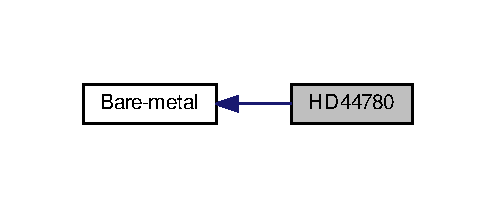
\includegraphics[width=238pt]{group___h_d44780}
\end{center}
\end{figure}
\subsection*{Strutture dati}
\begin{DoxyCompactItemize}
\item 
struct \hyperlink{struct_h_d44780___l_c_d__t}{H\+D44780\+\_\+\+L\+C\+D\+\_\+t}
\begin{DoxyCompactList}\small\item\em Struttura opaca che astrae un device Display L\+CD con cntroller Hitachi H\+D44780, o compatibile. Un oggetto di tipo \hyperlink{struct_h_d44780___l_c_d__t}{H\+D44780\+\_\+\+L\+C\+D\+\_\+t} rappresenta un device lcd H\+D44780. Il modulo è pensato per permettere la gestione di più display da parte dello stesso processore, agendo su oggetti \hyperlink{struct_h_d44780___l_c_d__t}{H\+D44780\+\_\+\+L\+C\+D\+\_\+t} diversi. Il modulo permette di utilizzare sia l\textquotesingle{}interfacciamento ad otto bit che quello a quattro bit, inizializzando il device opportunamente, attraverso l\textquotesingle{}uso delle funzioni H\+D44780\+\_\+\+Init8 e\+H\+D44780\+\_\+\+Init4. Il modulo fornisce anche semplici funzioni per la stampa di un carattere o di una stringa null-\/terminated di caratteri. Si veda la documentazione delle funzioni \hyperlink{group___h_d44780_ga57b8c6ca0b3c12e5f7273b3c373a6f17}{H\+D44780\+\_\+\+Printc()} e \hyperlink{group___h_d44780_ga3aedff8e2040e62db569fde955d3987b}{H\+D44780\+\_\+\+Print()}. Inoltre sono presenti diverse funzioni di utilità generica, come quelle per la pulizia del display, per lo spostamento del cursore di un posto in avanti o indietro, alla riga in basso o in alto. \end{DoxyCompactList}\end{DoxyCompactItemize}
\subsection*{Tipi enumerati (enum)}
\begin{DoxyCompactItemize}
\item 
enum \hyperlink{group___h_d44780_gaaaea8b73e24f7658da4118f6b01b45f0}{H\+D44780\+\_\+\+Interface\+Mode\+\_\+t} \{ \hyperlink{group___h_d44780_ggaaaea8b73e24f7658da4118f6b01b45f0a45bf6ce7ec7c951f692bdce9f0f485c6}{H\+D44780\+\_\+\+I\+N\+T\+E\+R\+F\+A\+C\+E\+\_\+4bit}, 
\hyperlink{group___h_d44780_ggaaaea8b73e24f7658da4118f6b01b45f0a24da9b234f9358c14184fe21f3c47de5}{H\+D44780\+\_\+\+I\+N\+T\+E\+R\+F\+A\+C\+E\+\_\+8bit}
 \}\begin{DoxyCompactList}\small\item\em Modalità di interfacciamento. Il modulo supporta sia interfacciamento a 4 bit che ad 8 bit. \end{DoxyCompactList}
\item 
enum \hyperlink{group___h_d44780_gaf46f4db4f981d3a1088804a6d6980d30}{H\+D44780\+\_\+\+Direction\+\_\+t} \{ \hyperlink{group___h_d44780_ggaf46f4db4f981d3a1088804a6d6980d30aa4d704398d4edd1e0dec8dbb55f90292}{H\+D44780\+\_\+\+Cursor\+Left}, 
\hyperlink{group___h_d44780_ggaf46f4db4f981d3a1088804a6d6980d30a26006ced693b6bab28c6e30bfdb8c399}{H\+D44780\+\_\+\+Cursor\+Right}
 \}\begin{DoxyCompactList}\small\item\em Direzioni di spostamento del cursore, usata dalla funzione \hyperlink{group___h_d44780_gabcea9a03050c46530e39b7556c673baf}{H\+D44780\+\_\+\+Move\+Cursor()} \end{DoxyCompactList}
\end{DoxyCompactItemize}
\subsection*{Funzioni}
\begin{DoxyCompactItemize}
\item 
void \hyperlink{group___h_d44780_gad212907e20316f4fc0e93d7c7a8f338e}{H\+D44780\+\_\+\+Init8} (\hyperlink{struct_h_d44780___l_c_d__t}{H\+D44780\+\_\+\+L\+C\+D\+\_\+t} $\ast$lcd, \hyperlink{structmy_g_p_i_o__t}{my\+G\+P\+I\+O\+\_\+t} $\ast$gpio, \hyperlink{group__bare-metal_ga402a0d20afc0cb7c25554b8b023f4253}{my\+G\+P\+I\+O\+\_\+mask} RS, \hyperlink{group__bare-metal_ga402a0d20afc0cb7c25554b8b023f4253}{my\+G\+P\+I\+O\+\_\+mask} RW, \hyperlink{group__bare-metal_ga402a0d20afc0cb7c25554b8b023f4253}{my\+G\+P\+I\+O\+\_\+mask} E, \hyperlink{group__bare-metal_ga402a0d20afc0cb7c25554b8b023f4253}{my\+G\+P\+I\+O\+\_\+mask} Data7, \hyperlink{group__bare-metal_ga402a0d20afc0cb7c25554b8b023f4253}{my\+G\+P\+I\+O\+\_\+mask} Data6, \hyperlink{group__bare-metal_ga402a0d20afc0cb7c25554b8b023f4253}{my\+G\+P\+I\+O\+\_\+mask} Data5, \hyperlink{group__bare-metal_ga402a0d20afc0cb7c25554b8b023f4253}{my\+G\+P\+I\+O\+\_\+mask} Data4, \hyperlink{group__bare-metal_ga402a0d20afc0cb7c25554b8b023f4253}{my\+G\+P\+I\+O\+\_\+mask} Data3, \hyperlink{group__bare-metal_ga402a0d20afc0cb7c25554b8b023f4253}{my\+G\+P\+I\+O\+\_\+mask} Data2, \hyperlink{group__bare-metal_ga402a0d20afc0cb7c25554b8b023f4253}{my\+G\+P\+I\+O\+\_\+mask} Data1, \hyperlink{group__bare-metal_ga402a0d20afc0cb7c25554b8b023f4253}{my\+G\+P\+I\+O\+\_\+mask} Data0)
\begin{DoxyCompactList}\small\item\em Inizializza un display lcd H\+D44780 con interfacciamento ad 8 bit. \end{DoxyCompactList}\item 
void \hyperlink{group___h_d44780_ga0c08f9e41d770ebfa4af385a56b47b81}{H\+D44780\+\_\+\+Init4} (\hyperlink{struct_h_d44780___l_c_d__t}{H\+D44780\+\_\+\+L\+C\+D\+\_\+t} $\ast$lcd, \hyperlink{structmy_g_p_i_o__t}{my\+G\+P\+I\+O\+\_\+t} $\ast$gpio, \hyperlink{group__bare-metal_ga402a0d20afc0cb7c25554b8b023f4253}{my\+G\+P\+I\+O\+\_\+mask} RS, \hyperlink{group__bare-metal_ga402a0d20afc0cb7c25554b8b023f4253}{my\+G\+P\+I\+O\+\_\+mask} RW, \hyperlink{group__bare-metal_ga402a0d20afc0cb7c25554b8b023f4253}{my\+G\+P\+I\+O\+\_\+mask} E, \hyperlink{group__bare-metal_ga402a0d20afc0cb7c25554b8b023f4253}{my\+G\+P\+I\+O\+\_\+mask} Data7, \hyperlink{group__bare-metal_ga402a0d20afc0cb7c25554b8b023f4253}{my\+G\+P\+I\+O\+\_\+mask} Data6, \hyperlink{group__bare-metal_ga402a0d20afc0cb7c25554b8b023f4253}{my\+G\+P\+I\+O\+\_\+mask} Data5, \hyperlink{group__bare-metal_ga402a0d20afc0cb7c25554b8b023f4253}{my\+G\+P\+I\+O\+\_\+mask} Data4)
\begin{DoxyCompactList}\small\item\em Inizializza un oggetto display lcd H\+D44780 affinché si utilizzi l\textquotesingle{}interfaccia a 4 bit. \end{DoxyCompactList}\item 
void \hyperlink{group___h_d44780_ga57b8c6ca0b3c12e5f7273b3c373a6f17}{H\+D44780\+\_\+\+Printc} (\hyperlink{struct_h_d44780___l_c_d__t}{H\+D44780\+\_\+\+L\+C\+D\+\_\+t} $\ast$lcd, char c)
\begin{DoxyCompactList}\small\item\em Stampa un carattere. \end{DoxyCompactList}\item 
void \hyperlink{group___h_d44780_ga3aedff8e2040e62db569fde955d3987b}{H\+D44780\+\_\+\+Print} (\hyperlink{struct_h_d44780___l_c_d__t}{H\+D44780\+\_\+\+L\+C\+D\+\_\+t} $\ast$lcd, const char $\ast$s)
\begin{DoxyCompactList}\small\item\em Stampa una stringa null-\/terminated di caratteri. \end{DoxyCompactList}\item 
void \hyperlink{group___h_d44780_ga2a5d4d528175321c46c790b581959e63}{H\+D44780\+\_\+print\+Binary8} (\hyperlink{struct_h_d44780___l_c_d__t}{H\+D44780\+\_\+\+L\+C\+D\+\_\+t} $\ast$lcd, uint8\+\_\+t b)
\begin{DoxyCompactList}\small\item\em Stampa un byte in binario. (bit più significativo a sinistra) \end{DoxyCompactList}\item 
void \hyperlink{group___h_d44780_ga95cceef2401c5519295e5a83c6688b5c}{H\+D44780\+\_\+print\+Binary32} (\hyperlink{struct_h_d44780___l_c_d__t}{H\+D44780\+\_\+\+L\+C\+D\+\_\+t} $\ast$lcd, uint32\+\_\+t w)
\begin{DoxyCompactList}\small\item\em Stampa una word di 32 bit in binario. (bit più significativo a sinistra) \end{DoxyCompactList}\item 
void \hyperlink{group___h_d44780_ga0f99bc5458acb172d0f3bfeb94f90e2a}{H\+D44780\+\_\+print\+Binary64} (\hyperlink{struct_h_d44780___l_c_d__t}{H\+D44780\+\_\+\+L\+C\+D\+\_\+t} $\ast$lcd, uint64\+\_\+t b)
\begin{DoxyCompactList}\small\item\em Stampa un blocco di 64 bit in binario. (bit più significativo a sinistra) \end{DoxyCompactList}\item 
void \hyperlink{group___h_d44780_gad967bd458b4d2bd358a93cbb7144addd}{H\+D44780\+\_\+print\+Hex8} (\hyperlink{struct_h_d44780___l_c_d__t}{H\+D44780\+\_\+\+L\+C\+D\+\_\+t} $\ast$lcd, uint8\+\_\+t b)
\begin{DoxyCompactList}\small\item\em Stampa un byte in esadecimale. (bit più significativo a sinistra) \end{DoxyCompactList}\item 
void \hyperlink{group___h_d44780_gaa82a2a27a3008f55c969a2d390c50497}{H\+D44780\+\_\+print\+Hex32} (\hyperlink{struct_h_d44780___l_c_d__t}{H\+D44780\+\_\+\+L\+C\+D\+\_\+t} $\ast$lcd, uint32\+\_\+t w)
\begin{DoxyCompactList}\small\item\em Stampa una word di 32 bit in esadecimale. (bit più significativo a sinistra) \end{DoxyCompactList}\item 
void \hyperlink{group___h_d44780_ga7a4b110e7da806f8c01e01d184d3a19a}{H\+D44780\+\_\+print\+Hex64} (\hyperlink{struct_h_d44780___l_c_d__t}{H\+D44780\+\_\+\+L\+C\+D\+\_\+t} $\ast$lcd, uint64\+\_\+t b)
\begin{DoxyCompactList}\small\item\em Stampa un blocco di 64 bit in esadecimale. (bit più significativo a sinistra) \end{DoxyCompactList}\item 
void \hyperlink{group___h_d44780_ga38cac13d7a66f068be54f79a716ff7d4}{H\+D44780\+\_\+\+Clear} (\hyperlink{struct_h_d44780___l_c_d__t}{H\+D44780\+\_\+\+L\+C\+D\+\_\+t} $\ast$lcd)
\begin{DoxyCompactList}\small\item\em Pulisce il display e sposta il cursore all\textquotesingle{}inizio della prima riga. \end{DoxyCompactList}\item 
void \hyperlink{group___h_d44780_ga68e3712332aa9482d4bdaa4991a92127}{H\+D44780\+\_\+\+Home} (\hyperlink{struct_h_d44780___l_c_d__t}{H\+D44780\+\_\+\+L\+C\+D\+\_\+t} $\ast$lcd)
\begin{DoxyCompactList}\small\item\em Sposta il cursore all\textquotesingle{}inizio della prima riga. \end{DoxyCompactList}\item 
void \hyperlink{group___h_d44780_gad90e2924a4e632ce42940323f8f49e37}{H\+D44780\+\_\+\+Move\+To\+Row1} (\hyperlink{struct_h_d44780___l_c_d__t}{H\+D44780\+\_\+\+L\+C\+D\+\_\+t} $\ast$lcd)
\begin{DoxyCompactList}\small\item\em Sposta il cursore all\textquotesingle{}inizio della prima riga. \end{DoxyCompactList}\item 
void \hyperlink{group___h_d44780_ga713670d498b6f5d50a174df19081c515}{H\+D44780\+\_\+\+Move\+To\+Row2} (\hyperlink{struct_h_d44780___l_c_d__t}{H\+D44780\+\_\+\+L\+C\+D\+\_\+t} $\ast$lcd)
\begin{DoxyCompactList}\small\item\em Sposta il cursore all\textquotesingle{}inizio della seconda riga. \end{DoxyCompactList}\item 
void \hyperlink{group___h_d44780_gabcea9a03050c46530e39b7556c673baf}{H\+D44780\+\_\+\+Move\+Cursor} (\hyperlink{struct_h_d44780___l_c_d__t}{H\+D44780\+\_\+\+L\+C\+D\+\_\+t} $\ast$lcd, \hyperlink{group___h_d44780_gaf46f4db4f981d3a1088804a6d6980d30}{H\+D44780\+\_\+\+Direction\+\_\+t} dir)
\begin{DoxyCompactList}\small\item\em Sposta il cursore di una posizione a destra o sinistra. \end{DoxyCompactList}\item 
void \hyperlink{group___h_d44780_ga5cf07b2179272029410f9a81f56621ed}{H\+D44780\+\_\+\+Display\+Off} (\hyperlink{struct_h_d44780___l_c_d__t}{H\+D44780\+\_\+\+L\+C\+D\+\_\+t} $\ast$lcd)
\begin{DoxyCompactList}\small\item\em Disattiva il display. \end{DoxyCompactList}\item 
void \hyperlink{group___h_d44780_ga56421dc398825188aa10257063a3ee4b}{H\+D44780\+\_\+\+Cursor\+Off} (\hyperlink{struct_h_d44780___l_c_d__t}{H\+D44780\+\_\+\+L\+C\+D\+\_\+t} $\ast$lcd)
\begin{DoxyCompactList}\small\item\em Disattiva la visualizzazione del cursore. \end{DoxyCompactList}\item 
void \hyperlink{group___h_d44780_ga3a381cb44df5d76d79be5ed71a52bae6}{H\+D44780\+\_\+\+Cursor\+On} (\hyperlink{struct_h_d44780___l_c_d__t}{H\+D44780\+\_\+\+L\+C\+D\+\_\+t} $\ast$lcd)
\begin{DoxyCompactList}\small\item\em Attiva la visualizzazione del cursore. \end{DoxyCompactList}\item 
void \hyperlink{group___h_d44780_ga92eb58cb7d73c9a87b7087a9c56f73d5}{H\+D44780\+\_\+\+Cursor\+Blink} (\hyperlink{struct_h_d44780___l_c_d__t}{H\+D44780\+\_\+\+L\+C\+D\+\_\+t} $\ast$lcd)
\begin{DoxyCompactList}\small\item\em Attiva il cursore lampeggiante. \end{DoxyCompactList}\end{DoxyCompactItemize}


\subsection{Descrizione dettagliata}
driver per display Hitachi hd44780 basato su driver my\+G\+P\+IO bare-\/metal 

Un oggetto di tipo \hyperlink{struct_h_d44780___l_c_d__t}{H\+D44780\+\_\+\+L\+C\+D\+\_\+t} rappresenta un device lcd H\+D44780. Il modulo è pensato per permettere la gestione di più display da parte dello stesso processore, agendo su oggetti \hyperlink{struct_h_d44780___l_c_d__t}{H\+D44780\+\_\+\+L\+C\+D\+\_\+t} diversi.~\newline
 La struttura \hyperlink{struct_h_d44780___l_c_d__t}{H\+D44780\+\_\+\+L\+C\+D\+\_\+t} specifica quali siano i pin del microcontrollore che pilotano un determinato segnale del device. L\textquotesingle{}assegnazione segnale-\/coppia, quindi l\textquotesingle{} inizializzazione della struttura \hyperlink{struct_h_d44780___l_c_d__t}{H\+D44780\+\_\+\+L\+C\+D\+\_\+t} relativa ad un device lcd, D\+E\+VE essere effettuata tassativamente utilizzando le funzioni~\newline

\begin{DoxyItemize}
\item \hyperlink{group___h_d44780_ga0c08f9e41d770ebfa4af385a56b47b81}{H\+D44780\+\_\+\+Init4()}
\item \hyperlink{group___h_d44780_gad212907e20316f4fc0e93d7c7a8f338e}{H\+D44780\+\_\+\+Init8()}~\newline

\end{DoxyItemize}

le quali provvedono anche ad effettuare un test di connessione volto ad individuare eventuali segnali erroneamente associati.~\newline


Oltre alle funzioni di inizializzazione, il modulo fornisce anche funzioni basilari per la stampa su display lcd di
\begin{DoxyItemize}
\item caratteri, con la funzione \hyperlink{group___h_d44780_ga57b8c6ca0b3c12e5f7273b3c373a6f17}{H\+D44780\+\_\+\+Printc()}
\item stringhe null-\/terminated di caratteri, con la funzione \hyperlink{group___h_d44780_ga3aedff8e2040e62db569fde955d3987b}{H\+D44780\+\_\+\+Print()}~\newline

\end{DoxyItemize}

Sono disponibili, inoltre, anche funzioni specifiche per inviare comandi al device\+:
\begin{DoxyItemize}
\item \hyperlink{group___h_d44780_ga38cac13d7a66f068be54f79a716ff7d4}{H\+D44780\+\_\+\+Clear()}
\item \hyperlink{group___h_d44780_ga68e3712332aa9482d4bdaa4991a92127}{H\+D44780\+\_\+\+Home()}
\item \hyperlink{group___h_d44780_gad90e2924a4e632ce42940323f8f49e37}{H\+D44780\+\_\+\+Move\+To\+Row1()}
\item \hyperlink{group___h_d44780_ga713670d498b6f5d50a174df19081c515}{H\+D44780\+\_\+\+Move\+To\+Row2()}
\item \hyperlink{group___h_d44780_gabcea9a03050c46530e39b7556c673baf}{H\+D44780\+\_\+\+Move\+Cursor()}
\item \hyperlink{group___h_d44780_ga5cf07b2179272029410f9a81f56621ed}{H\+D44780\+\_\+\+Display\+Off()}
\item \hyperlink{group___h_d44780_ga56421dc398825188aa10257063a3ee4b}{H\+D44780\+\_\+\+Cursor\+Off()}
\item \hyperlink{group___h_d44780_ga3a381cb44df5d76d79be5ed71a52bae6}{H\+D44780\+\_\+\+Cursor\+On()}
\item \hyperlink{group___h_d44780_ga92eb58cb7d73c9a87b7087a9c56f73d5}{H\+D44780\+\_\+\+Cursor\+Blink()}~\newline
 
\end{DoxyItemize}

\subsection{Documentazione dei tipi enumerati}
\mbox{\Hypertarget{group___h_d44780_gaf46f4db4f981d3a1088804a6d6980d30}\label{group___h_d44780_gaf46f4db4f981d3a1088804a6d6980d30}} 
\index{H\+D44780@{H\+D44780}!H\+D44780\+\_\+\+Direction\+\_\+t@{H\+D44780\+\_\+\+Direction\+\_\+t}}
\index{H\+D44780\+\_\+\+Direction\+\_\+t@{H\+D44780\+\_\+\+Direction\+\_\+t}!H\+D44780@{H\+D44780}}
\subsubsection{\texorpdfstring{H\+D44780\+\_\+\+Direction\+\_\+t}{HD44780\_Direction\_t}}
{\footnotesize\ttfamily enum \hyperlink{group___h_d44780_gaf46f4db4f981d3a1088804a6d6980d30}{H\+D44780\+\_\+\+Direction\+\_\+t}}



Direzioni di spostamento del cursore, usata dalla funzione \hyperlink{group___h_d44780_gabcea9a03050c46530e39b7556c673baf}{H\+D44780\+\_\+\+Move\+Cursor()} 

\begin{DoxyEnumFields}{Valori del tipo enumerato}
\raisebox{\heightof{T}}[0pt][0pt]{\index{H\+D44780\+\_\+\+Cursor\+Left@{H\+D44780\+\_\+\+Cursor\+Left}!H\+D44780@{H\+D44780}}\index{H\+D44780@{H\+D44780}!H\+D44780\+\_\+\+Cursor\+Left@{H\+D44780\+\_\+\+Cursor\+Left}}}\mbox{\Hypertarget{group___h_d44780_ggaf46f4db4f981d3a1088804a6d6980d30aa4d704398d4edd1e0dec8dbb55f90292}\label{group___h_d44780_ggaf46f4db4f981d3a1088804a6d6980d30aa4d704398d4edd1e0dec8dbb55f90292}} 
H\+D44780\+\_\+\+Cursor\+Left&left sposta il cursore a sinistra \\
\hline

\raisebox{\heightof{T}}[0pt][0pt]{\index{H\+D44780\+\_\+\+Cursor\+Right@{H\+D44780\+\_\+\+Cursor\+Right}!H\+D44780@{H\+D44780}}\index{H\+D44780@{H\+D44780}!H\+D44780\+\_\+\+Cursor\+Right@{H\+D44780\+\_\+\+Cursor\+Right}}}\mbox{\Hypertarget{group___h_d44780_ggaf46f4db4f981d3a1088804a6d6980d30a26006ced693b6bab28c6e30bfdb8c399}\label{group___h_d44780_ggaf46f4db4f981d3a1088804a6d6980d30a26006ced693b6bab28c6e30bfdb8c399}} 
H\+D44780\+\_\+\+Cursor\+Right&right sposta il cursore a destra \\
\hline

\end{DoxyEnumFields}
\mbox{\Hypertarget{group___h_d44780_gaaaea8b73e24f7658da4118f6b01b45f0}\label{group___h_d44780_gaaaea8b73e24f7658da4118f6b01b45f0}} 
\index{H\+D44780@{H\+D44780}!H\+D44780\+\_\+\+Interface\+Mode\+\_\+t@{H\+D44780\+\_\+\+Interface\+Mode\+\_\+t}}
\index{H\+D44780\+\_\+\+Interface\+Mode\+\_\+t@{H\+D44780\+\_\+\+Interface\+Mode\+\_\+t}!H\+D44780@{H\+D44780}}
\subsubsection{\texorpdfstring{H\+D44780\+\_\+\+Interface\+Mode\+\_\+t}{HD44780\_InterfaceMode\_t}}
{\footnotesize\ttfamily enum \hyperlink{group___h_d44780_gaaaea8b73e24f7658da4118f6b01b45f0}{H\+D44780\+\_\+\+Interface\+Mode\+\_\+t}}



Modalità di interfacciamento. Il modulo supporta sia interfacciamento a 4 bit che ad 8 bit. 

\begin{DoxyEnumFields}{Valori del tipo enumerato}
\raisebox{\heightof{T}}[0pt][0pt]{\index{H\+D44780\+\_\+\+I\+N\+T\+E\+R\+F\+A\+C\+E\+\_\+4bit@{H\+D44780\+\_\+\+I\+N\+T\+E\+R\+F\+A\+C\+E\+\_\+4bit}!H\+D44780@{H\+D44780}}\index{H\+D44780@{H\+D44780}!H\+D44780\+\_\+\+I\+N\+T\+E\+R\+F\+A\+C\+E\+\_\+4bit@{H\+D44780\+\_\+\+I\+N\+T\+E\+R\+F\+A\+C\+E\+\_\+4bit}}}\mbox{\Hypertarget{group___h_d44780_ggaaaea8b73e24f7658da4118f6b01b45f0a45bf6ce7ec7c951f692bdce9f0f485c6}\label{group___h_d44780_ggaaaea8b73e24f7658da4118f6b01b45f0a45bf6ce7ec7c951f692bdce9f0f485c6}} 
H\+D44780\+\_\+\+I\+N\+T\+E\+R\+F\+A\+C\+E\+\_\+4bit&Interfacciamento a quattro bit \\
\hline

\raisebox{\heightof{T}}[0pt][0pt]{\index{H\+D44780\+\_\+\+I\+N\+T\+E\+R\+F\+A\+C\+E\+\_\+8bit@{H\+D44780\+\_\+\+I\+N\+T\+E\+R\+F\+A\+C\+E\+\_\+8bit}!H\+D44780@{H\+D44780}}\index{H\+D44780@{H\+D44780}!H\+D44780\+\_\+\+I\+N\+T\+E\+R\+F\+A\+C\+E\+\_\+8bit@{H\+D44780\+\_\+\+I\+N\+T\+E\+R\+F\+A\+C\+E\+\_\+8bit}}}\mbox{\Hypertarget{group___h_d44780_ggaaaea8b73e24f7658da4118f6b01b45f0a24da9b234f9358c14184fe21f3c47de5}\label{group___h_d44780_ggaaaea8b73e24f7658da4118f6b01b45f0a24da9b234f9358c14184fe21f3c47de5}} 
H\+D44780\+\_\+\+I\+N\+T\+E\+R\+F\+A\+C\+E\+\_\+8bit&Interfacciamento ad otto bit \\
\hline

\end{DoxyEnumFields}


\subsection{Documentazione delle funzioni}
\mbox{\Hypertarget{group___h_d44780_ga38cac13d7a66f068be54f79a716ff7d4}\label{group___h_d44780_ga38cac13d7a66f068be54f79a716ff7d4}} 
\index{H\+D44780@{H\+D44780}!H\+D44780\+\_\+\+Clear@{H\+D44780\+\_\+\+Clear}}
\index{H\+D44780\+\_\+\+Clear@{H\+D44780\+\_\+\+Clear}!H\+D44780@{H\+D44780}}
\subsubsection{\texorpdfstring{H\+D44780\+\_\+\+Clear()}{HD44780\_Clear()}}
{\footnotesize\ttfamily void H\+D44780\+\_\+\+Clear (\begin{DoxyParamCaption}\item[{\hyperlink{struct_h_d44780___l_c_d__t}{H\+D44780\+\_\+\+L\+C\+D\+\_\+t} $\ast$}]{lcd }\end{DoxyParamCaption})}



Pulisce il display e sposta il cursore all\textquotesingle{}inizio della prima riga. 


\begin{DoxyParams}[1]{Parametri}
\mbox{\tt in}  & {\em lcd} & display da pilotare; \\
\hline
\end{DoxyParams}
\mbox{\Hypertarget{group___h_d44780_ga92eb58cb7d73c9a87b7087a9c56f73d5}\label{group___h_d44780_ga92eb58cb7d73c9a87b7087a9c56f73d5}} 
\index{H\+D44780@{H\+D44780}!H\+D44780\+\_\+\+Cursor\+Blink@{H\+D44780\+\_\+\+Cursor\+Blink}}
\index{H\+D44780\+\_\+\+Cursor\+Blink@{H\+D44780\+\_\+\+Cursor\+Blink}!H\+D44780@{H\+D44780}}
\subsubsection{\texorpdfstring{H\+D44780\+\_\+\+Cursor\+Blink()}{HD44780\_CursorBlink()}}
{\footnotesize\ttfamily void H\+D44780\+\_\+\+Cursor\+Blink (\begin{DoxyParamCaption}\item[{\hyperlink{struct_h_d44780___l_c_d__t}{H\+D44780\+\_\+\+L\+C\+D\+\_\+t} $\ast$}]{lcd }\end{DoxyParamCaption})}



Attiva il cursore lampeggiante. 


\begin{DoxyParams}[1]{Parametri}
\mbox{\tt in}  & {\em lcd} & display da pilotare; \\
\hline
\end{DoxyParams}
\mbox{\Hypertarget{group___h_d44780_ga56421dc398825188aa10257063a3ee4b}\label{group___h_d44780_ga56421dc398825188aa10257063a3ee4b}} 
\index{H\+D44780@{H\+D44780}!H\+D44780\+\_\+\+Cursor\+Off@{H\+D44780\+\_\+\+Cursor\+Off}}
\index{H\+D44780\+\_\+\+Cursor\+Off@{H\+D44780\+\_\+\+Cursor\+Off}!H\+D44780@{H\+D44780}}
\subsubsection{\texorpdfstring{H\+D44780\+\_\+\+Cursor\+Off()}{HD44780\_CursorOff()}}
{\footnotesize\ttfamily void H\+D44780\+\_\+\+Cursor\+Off (\begin{DoxyParamCaption}\item[{\hyperlink{struct_h_d44780___l_c_d__t}{H\+D44780\+\_\+\+L\+C\+D\+\_\+t} $\ast$}]{lcd }\end{DoxyParamCaption})}



Disattiva la visualizzazione del cursore. 


\begin{DoxyParams}[1]{Parametri}
\mbox{\tt in}  & {\em lcd} & display da pilotare; \\
\hline
\end{DoxyParams}
\mbox{\Hypertarget{group___h_d44780_ga3a381cb44df5d76d79be5ed71a52bae6}\label{group___h_d44780_ga3a381cb44df5d76d79be5ed71a52bae6}} 
\index{H\+D44780@{H\+D44780}!H\+D44780\+\_\+\+Cursor\+On@{H\+D44780\+\_\+\+Cursor\+On}}
\index{H\+D44780\+\_\+\+Cursor\+On@{H\+D44780\+\_\+\+Cursor\+On}!H\+D44780@{H\+D44780}}
\subsubsection{\texorpdfstring{H\+D44780\+\_\+\+Cursor\+On()}{HD44780\_CursorOn()}}
{\footnotesize\ttfamily void H\+D44780\+\_\+\+Cursor\+On (\begin{DoxyParamCaption}\item[{\hyperlink{struct_h_d44780___l_c_d__t}{H\+D44780\+\_\+\+L\+C\+D\+\_\+t} $\ast$}]{lcd }\end{DoxyParamCaption})}



Attiva la visualizzazione del cursore. 


\begin{DoxyParams}[1]{Parametri}
\mbox{\tt in}  & {\em lcd} & display da pilotare; \\
\hline
\end{DoxyParams}
\mbox{\Hypertarget{group___h_d44780_ga5cf07b2179272029410f9a81f56621ed}\label{group___h_d44780_ga5cf07b2179272029410f9a81f56621ed}} 
\index{H\+D44780@{H\+D44780}!H\+D44780\+\_\+\+Display\+Off@{H\+D44780\+\_\+\+Display\+Off}}
\index{H\+D44780\+\_\+\+Display\+Off@{H\+D44780\+\_\+\+Display\+Off}!H\+D44780@{H\+D44780}}
\subsubsection{\texorpdfstring{H\+D44780\+\_\+\+Display\+Off()}{HD44780\_DisplayOff()}}
{\footnotesize\ttfamily void H\+D44780\+\_\+\+Display\+Off (\begin{DoxyParamCaption}\item[{\hyperlink{struct_h_d44780___l_c_d__t}{H\+D44780\+\_\+\+L\+C\+D\+\_\+t} $\ast$}]{lcd }\end{DoxyParamCaption})}



Disattiva il display. 


\begin{DoxyParams}[1]{Parametri}
\mbox{\tt in}  & {\em lcd} & display da pilotare; \\
\hline
\end{DoxyParams}
\mbox{\Hypertarget{group___h_d44780_ga68e3712332aa9482d4bdaa4991a92127}\label{group___h_d44780_ga68e3712332aa9482d4bdaa4991a92127}} 
\index{H\+D44780@{H\+D44780}!H\+D44780\+\_\+\+Home@{H\+D44780\+\_\+\+Home}}
\index{H\+D44780\+\_\+\+Home@{H\+D44780\+\_\+\+Home}!H\+D44780@{H\+D44780}}
\subsubsection{\texorpdfstring{H\+D44780\+\_\+\+Home()}{HD44780\_Home()}}
{\footnotesize\ttfamily void H\+D44780\+\_\+\+Home (\begin{DoxyParamCaption}\item[{\hyperlink{struct_h_d44780___l_c_d__t}{H\+D44780\+\_\+\+L\+C\+D\+\_\+t} $\ast$}]{lcd }\end{DoxyParamCaption})}



Sposta il cursore all\textquotesingle{}inizio della prima riga. 


\begin{DoxyParams}[1]{Parametri}
\mbox{\tt in}  & {\em lcd} & display da pilotare; \\
\hline
\end{DoxyParams}
\mbox{\Hypertarget{group___h_d44780_ga0c08f9e41d770ebfa4af385a56b47b81}\label{group___h_d44780_ga0c08f9e41d770ebfa4af385a56b47b81}} 
\index{H\+D44780@{H\+D44780}!H\+D44780\+\_\+\+Init4@{H\+D44780\+\_\+\+Init4}}
\index{H\+D44780\+\_\+\+Init4@{H\+D44780\+\_\+\+Init4}!H\+D44780@{H\+D44780}}
\subsubsection{\texorpdfstring{H\+D44780\+\_\+\+Init4()}{HD44780\_Init4()}}
{\footnotesize\ttfamily void H\+D44780\+\_\+\+Init4 (\begin{DoxyParamCaption}\item[{\hyperlink{struct_h_d44780___l_c_d__t}{H\+D44780\+\_\+\+L\+C\+D\+\_\+t} $\ast$}]{lcd,  }\item[{\hyperlink{structmy_g_p_i_o__t}{my\+G\+P\+I\+O\+\_\+t} $\ast$}]{gpio,  }\item[{\hyperlink{group__bare-metal_ga402a0d20afc0cb7c25554b8b023f4253}{my\+G\+P\+I\+O\+\_\+mask}}]{RS,  }\item[{\hyperlink{group__bare-metal_ga402a0d20afc0cb7c25554b8b023f4253}{my\+G\+P\+I\+O\+\_\+mask}}]{RW,  }\item[{\hyperlink{group__bare-metal_ga402a0d20afc0cb7c25554b8b023f4253}{my\+G\+P\+I\+O\+\_\+mask}}]{E,  }\item[{\hyperlink{group__bare-metal_ga402a0d20afc0cb7c25554b8b023f4253}{my\+G\+P\+I\+O\+\_\+mask}}]{Data7,  }\item[{\hyperlink{group__bare-metal_ga402a0d20afc0cb7c25554b8b023f4253}{my\+G\+P\+I\+O\+\_\+mask}}]{Data6,  }\item[{\hyperlink{group__bare-metal_ga402a0d20afc0cb7c25554b8b023f4253}{my\+G\+P\+I\+O\+\_\+mask}}]{Data5,  }\item[{\hyperlink{group__bare-metal_ga402a0d20afc0cb7c25554b8b023f4253}{my\+G\+P\+I\+O\+\_\+mask}}]{Data4 }\end{DoxyParamCaption})}



Inizializza un oggetto display lcd H\+D44780 affinché si utilizzi l\textquotesingle{}interfaccia a 4 bit. 

Inizializza un oggetto \hyperlink{struct_h_d44780___l_c_d__t}{H\+D44780\+\_\+\+L\+C\+D\+\_\+t} verificando la validità delle coppie porta-\/pin per l\textquotesingle{} interfacciamento, configurando i pin my\+G\+P\+IO e inizializzando il device.

\begin{DoxyWarning}{Avvertimento}
Se i pin associati ai segnali di pilotaggio del device non sono correttamente configurati come pin di output, il dispositivo non funzionerà correttamente.

Non modificare i campi della struttura \hyperlink{struct_h_d44780___l_c_d__t}{H\+D44780\+\_\+\+L\+C\+D\+\_\+t} dopo che essa sia stata inizializzata.

La struttura \hyperlink{structmy_g_p_i_o__t}{my\+G\+P\+I\+O\+\_\+t}, a cui fa riferimento il parametro gpio, va inizializzata a parte.
\end{DoxyWarning}

\begin{DoxyParams}[1]{Parametri}
\mbox{\tt in,out}  & {\em lcd} & puntatore a struttura di tipo \hyperlink{struct_h_d44780___l_c_d__t}{H\+D44780\+\_\+\+L\+C\+D\+\_\+t} che descrive un display H\+D44780 da inizializzare; \\
\hline
\mbox{\tt in}  & {\em gpio} & puntatore alla struttura \hyperlink{structmy_g_p_i_o__t}{my\+G\+P\+I\+O\+\_\+t} che astrae il device my\+G\+P\+IO a cui il display è connesso. Non viene inizializzato dalla funziona, sarà necessario inizializzarlo preventivamente; \\
\hline
\mbox{\tt in}  & {\em RS} & pin del device my\+G\+P\+IO a cui è associato il segnale RS (data/command) del display L\+CD; \\
\hline
\mbox{\tt in}  & {\em RW} & pin del device my\+G\+P\+IO a cui è associato il segnale RW (read/write) del display L\+CD; \\
\hline
\mbox{\tt in}  & {\em E} & pin del device my\+G\+P\+IO a cui è associato il segnale E (Enable) del display L\+CD; \\
\hline
\mbox{\tt in}  & {\em Data7} & pin del device my\+G\+P\+IO a cui è associato il segnale Data7 del display L\+CD; \\
\hline
\mbox{\tt in}  & {\em Data6} & pin del device my\+G\+P\+IO a cui è associato il segnale Data6 del display L\+CD; \\
\hline
\mbox{\tt in}  & {\em Data5} & pin del device my\+G\+P\+IO a cui è associato il segnale Data5 del display L\+CD; \\
\hline
\mbox{\tt in}  & {\em Data4} & pin del device my\+G\+P\+IO a cui è associato il segnale Data4 del display L\+CD;\\
\hline
\end{DoxyParams}

\begin{DoxyCode}
\hyperlink{structmy_g_p_i_o__t}{myGPIO\_t} gpioDisplay;
GPIO\_init(&gpioDisplay, XPAR\_MYGPIO\_3\_S00\_AXI\_BASEADDR, 11, 0, 4, 8);
\hyperlink{struct_h_d44780___l_c_d__t}{HD44780\_LCD\_t} lcd;
\hyperlink{group___h_d44780_ga0c08f9e41d770ebfa4af385a56b47b81}{HD44780\_Init4}(&lcd, &gpioDisplay,   GPIO\_pin10, GPIO\_pin9, GPIO\_pin8,
                                        GPIO\_pin0, GPIO\_pin1, GPIO\_pin2, GPIO\_pin3);
\hyperlink{group___h_d44780_ga3aedff8e2040e62db569fde955d3987b}{HD44780\_Print}(&lcd, \textcolor{stringliteral}{"Ciao! Come va"});
\hyperlink{group___h_d44780_ga713670d498b6f5d50a174df19081c515}{HD44780\_MoveToRow2}(&lcd);
\hyperlink{group___h_d44780_ga3aedff8e2040e62db569fde955d3987b}{HD44780\_Print}(&lcd, \textcolor{stringliteral}{"lo studio?"});
\end{DoxyCode}
 \mbox{\Hypertarget{group___h_d44780_gad212907e20316f4fc0e93d7c7a8f338e}\label{group___h_d44780_gad212907e20316f4fc0e93d7c7a8f338e}} 
\index{H\+D44780@{H\+D44780}!H\+D44780\+\_\+\+Init8@{H\+D44780\+\_\+\+Init8}}
\index{H\+D44780\+\_\+\+Init8@{H\+D44780\+\_\+\+Init8}!H\+D44780@{H\+D44780}}
\subsubsection{\texorpdfstring{H\+D44780\+\_\+\+Init8()}{HD44780\_Init8()}}
{\footnotesize\ttfamily void H\+D44780\+\_\+\+Init8 (\begin{DoxyParamCaption}\item[{\hyperlink{struct_h_d44780___l_c_d__t}{H\+D44780\+\_\+\+L\+C\+D\+\_\+t} $\ast$}]{lcd,  }\item[{\hyperlink{structmy_g_p_i_o__t}{my\+G\+P\+I\+O\+\_\+t} $\ast$}]{gpio,  }\item[{\hyperlink{group__bare-metal_ga402a0d20afc0cb7c25554b8b023f4253}{my\+G\+P\+I\+O\+\_\+mask}}]{RS,  }\item[{\hyperlink{group__bare-metal_ga402a0d20afc0cb7c25554b8b023f4253}{my\+G\+P\+I\+O\+\_\+mask}}]{RW,  }\item[{\hyperlink{group__bare-metal_ga402a0d20afc0cb7c25554b8b023f4253}{my\+G\+P\+I\+O\+\_\+mask}}]{E,  }\item[{\hyperlink{group__bare-metal_ga402a0d20afc0cb7c25554b8b023f4253}{my\+G\+P\+I\+O\+\_\+mask}}]{Data7,  }\item[{\hyperlink{group__bare-metal_ga402a0d20afc0cb7c25554b8b023f4253}{my\+G\+P\+I\+O\+\_\+mask}}]{Data6,  }\item[{\hyperlink{group__bare-metal_ga402a0d20afc0cb7c25554b8b023f4253}{my\+G\+P\+I\+O\+\_\+mask}}]{Data5,  }\item[{\hyperlink{group__bare-metal_ga402a0d20afc0cb7c25554b8b023f4253}{my\+G\+P\+I\+O\+\_\+mask}}]{Data4,  }\item[{\hyperlink{group__bare-metal_ga402a0d20afc0cb7c25554b8b023f4253}{my\+G\+P\+I\+O\+\_\+mask}}]{Data3,  }\item[{\hyperlink{group__bare-metal_ga402a0d20afc0cb7c25554b8b023f4253}{my\+G\+P\+I\+O\+\_\+mask}}]{Data2,  }\item[{\hyperlink{group__bare-metal_ga402a0d20afc0cb7c25554b8b023f4253}{my\+G\+P\+I\+O\+\_\+mask}}]{Data1,  }\item[{\hyperlink{group__bare-metal_ga402a0d20afc0cb7c25554b8b023f4253}{my\+G\+P\+I\+O\+\_\+mask}}]{Data0 }\end{DoxyParamCaption})}



Inizializza un display lcd H\+D44780 con interfacciamento ad 8 bit. 

\begin{DoxyWarning}{Avvertimento}
Se i pin associati ai segnali di pilotaggio del device non sono correttamente configurati come pin di output, il dispositivo non funzionerà correttamente.

Non modificare i campi della struttura dopo che essa sia stata inizializzata.

La struttura \hyperlink{structmy_g_p_i_o__t}{my\+G\+P\+I\+O\+\_\+t}, a cui fa riferimento il parametro gpio, va inizializzata a parte.
\end{DoxyWarning}

\begin{DoxyParams}[1]{Parametri}
\mbox{\tt in,out}  & {\em lcd} & puntatore a struttura di tipo \hyperlink{struct_h_d44780___l_c_d__t}{H\+D44780\+\_\+\+L\+C\+D\+\_\+t} che descrive un display H\+D44780 da inizializzare; \\
\hline
\mbox{\tt in}  & {\em gpio} & puntatore alla struttura \hyperlink{structmy_g_p_i_o__t}{my\+G\+P\+I\+O\+\_\+t} che astrae il device my\+G\+P\+IO a cui il display è connesso. Non viene inizializzato dalla funziona, sarà necessario inizializzarlo preventivamente; \\
\hline
\mbox{\tt in}  & {\em RS} & pin del device my\+G\+P\+IO a cui è associato il segnale RS (data/command) del display L\+CD; \\
\hline
\mbox{\tt in}  & {\em RW} & pin del device my\+G\+P\+IO a cui è associato il segnale RW (read/write) del display L\+CD; \\
\hline
\mbox{\tt in}  & {\em E} & pin del device my\+G\+P\+IO a cui è associato il segnale E (Enable) del display L\+CD; \\
\hline
\mbox{\tt in}  & {\em Data7} & pin del device my\+G\+P\+IO a cui è associato il segnale Data7 del display L\+CD; \\
\hline
\mbox{\tt in}  & {\em Data6} & pin del device my\+G\+P\+IO a cui è associato il segnale Data6 del display L\+CD; \\
\hline
\mbox{\tt in}  & {\em Data5} & pin del device my\+G\+P\+IO a cui è associato il segnale Data5 del display L\+CD; \\
\hline
\mbox{\tt in}  & {\em Data4} & pin del device my\+G\+P\+IO a cui è associato il segnale Data4 del display L\+CD; \\
\hline
\mbox{\tt in}  & {\em Data3} & pin del device my\+G\+P\+IO a cui è associato il segnale Data3 del display L\+CD; \\
\hline
\mbox{\tt in}  & {\em Data2} & pin del device my\+G\+P\+IO a cui è associato il segnale Data2 del display L\+CD; \\
\hline
\mbox{\tt in}  & {\em Data1} & pin del device my\+G\+P\+IO a cui è associato il segnale Data1 del display L\+CD; \\
\hline
\mbox{\tt in}  & {\em Data0} & pin del device my\+G\+P\+IO a cui è associato il segnale Data0 del display L\+CD;\\
\hline
\end{DoxyParams}

\begin{DoxyCode}
\hyperlink{structmy_g_p_i_o__t}{myGPIO\_t} gpioDisplay;
\hyperlink{group__bare-metal_ga588201358d1633c53535b288c9198531}{myGPIO\_Init}(&gpioDisplay, XPAR\_MYGPIO\_3\_S00\_AXI\_BASEADDR);
\hyperlink{struct_h_d44780___l_c_d__t}{HD44780\_LCD\_t} lcd;
\hyperlink{group___h_d44780_gad212907e20316f4fc0e93d7c7a8f338e}{HD44780\_Init8}(&lcd, &gpioDisplay,   GPIO\_pin10, GPIO\_pin9, GPIO\_pin8,
                                        GPIO\_pin0, GPIO\_pin1, GPIO\_pin2, GPIO\_pin3,
                                    GPIO\_pin4, GPIO\_pin5, GPIO\_pin6, GPIO\_pin7);
\hyperlink{group___h_d44780_ga3aedff8e2040e62db569fde955d3987b}{HD44780\_Print}(&lcd, \textcolor{stringliteral}{"Ciao! Come va"});
\hyperlink{group___h_d44780_ga713670d498b6f5d50a174df19081c515}{HD44780\_MoveToRow2}(&lcd);
\hyperlink{group___h_d44780_ga3aedff8e2040e62db569fde955d3987b}{HD44780\_Print}(&lcd, \textcolor{stringliteral}{"lo studio?"});
\end{DoxyCode}
 \mbox{\Hypertarget{group___h_d44780_gabcea9a03050c46530e39b7556c673baf}\label{group___h_d44780_gabcea9a03050c46530e39b7556c673baf}} 
\index{H\+D44780@{H\+D44780}!H\+D44780\+\_\+\+Move\+Cursor@{H\+D44780\+\_\+\+Move\+Cursor}}
\index{H\+D44780\+\_\+\+Move\+Cursor@{H\+D44780\+\_\+\+Move\+Cursor}!H\+D44780@{H\+D44780}}
\subsubsection{\texorpdfstring{H\+D44780\+\_\+\+Move\+Cursor()}{HD44780\_MoveCursor()}}
{\footnotesize\ttfamily void H\+D44780\+\_\+\+Move\+Cursor (\begin{DoxyParamCaption}\item[{\hyperlink{struct_h_d44780___l_c_d__t}{H\+D44780\+\_\+\+L\+C\+D\+\_\+t} $\ast$}]{lcd,  }\item[{\hyperlink{group___h_d44780_gaf46f4db4f981d3a1088804a6d6980d30}{H\+D44780\+\_\+\+Direction\+\_\+t}}]{dir }\end{DoxyParamCaption})}



Sposta il cursore di una posizione a destra o sinistra. 


\begin{DoxyParams}[1]{Parametri}
\mbox{\tt in}  & {\em lcd} & display da pilotare; \\
\hline
\mbox{\tt in}  & {\em dir} & direzione in cui spostare il cursore, \\
\hline
\end{DoxyParams}
\begin{DoxySeeAlso}{Si veda anche}
direction\+\_\+t; 
\end{DoxySeeAlso}
\mbox{\Hypertarget{group___h_d44780_gad90e2924a4e632ce42940323f8f49e37}\label{group___h_d44780_gad90e2924a4e632ce42940323f8f49e37}} 
\index{H\+D44780@{H\+D44780}!H\+D44780\+\_\+\+Move\+To\+Row1@{H\+D44780\+\_\+\+Move\+To\+Row1}}
\index{H\+D44780\+\_\+\+Move\+To\+Row1@{H\+D44780\+\_\+\+Move\+To\+Row1}!H\+D44780@{H\+D44780}}
\subsubsection{\texorpdfstring{H\+D44780\+\_\+\+Move\+To\+Row1()}{HD44780\_MoveToRow1()}}
{\footnotesize\ttfamily void H\+D44780\+\_\+\+Move\+To\+Row1 (\begin{DoxyParamCaption}\item[{\hyperlink{struct_h_d44780___l_c_d__t}{H\+D44780\+\_\+\+L\+C\+D\+\_\+t} $\ast$}]{lcd }\end{DoxyParamCaption})}



Sposta il cursore all\textquotesingle{}inizio della prima riga. 


\begin{DoxyParams}[1]{Parametri}
\mbox{\tt in}  & {\em lcd} & display da pilotare; \\
\hline
\end{DoxyParams}
\mbox{\Hypertarget{group___h_d44780_ga713670d498b6f5d50a174df19081c515}\label{group___h_d44780_ga713670d498b6f5d50a174df19081c515}} 
\index{H\+D44780@{H\+D44780}!H\+D44780\+\_\+\+Move\+To\+Row2@{H\+D44780\+\_\+\+Move\+To\+Row2}}
\index{H\+D44780\+\_\+\+Move\+To\+Row2@{H\+D44780\+\_\+\+Move\+To\+Row2}!H\+D44780@{H\+D44780}}
\subsubsection{\texorpdfstring{H\+D44780\+\_\+\+Move\+To\+Row2()}{HD44780\_MoveToRow2()}}
{\footnotesize\ttfamily void H\+D44780\+\_\+\+Move\+To\+Row2 (\begin{DoxyParamCaption}\item[{\hyperlink{struct_h_d44780___l_c_d__t}{H\+D44780\+\_\+\+L\+C\+D\+\_\+t} $\ast$}]{lcd }\end{DoxyParamCaption})}



Sposta il cursore all\textquotesingle{}inizio della seconda riga. 


\begin{DoxyParams}[1]{Parametri}
\mbox{\tt in}  & {\em lcd} & display da pilotare; \\
\hline
\end{DoxyParams}
\mbox{\Hypertarget{group___h_d44780_ga3aedff8e2040e62db569fde955d3987b}\label{group___h_d44780_ga3aedff8e2040e62db569fde955d3987b}} 
\index{H\+D44780@{H\+D44780}!H\+D44780\+\_\+\+Print@{H\+D44780\+\_\+\+Print}}
\index{H\+D44780\+\_\+\+Print@{H\+D44780\+\_\+\+Print}!H\+D44780@{H\+D44780}}
\subsubsection{\texorpdfstring{H\+D44780\+\_\+\+Print()}{HD44780\_Print()}}
{\footnotesize\ttfamily void H\+D44780\+\_\+\+Print (\begin{DoxyParamCaption}\item[{\hyperlink{struct_h_d44780___l_c_d__t}{H\+D44780\+\_\+\+L\+C\+D\+\_\+t} $\ast$}]{lcd,  }\item[{const char $\ast$}]{s }\end{DoxyParamCaption})}



Stampa una stringa null-\/terminated di caratteri. 

La funzione può essere utilizzata per stampare anche numeri interi e floating point. Si veda gli esempi di cui sotto.


\begin{DoxyParams}[1]{Parametri}
\mbox{\tt in}  & {\em lcd} & display da pilotare; \\
\hline
\mbox{\tt in}  & {\em s} & puntatore alla stringa null-\/terminated da stampare sul display;\\
\hline
\end{DoxyParams}

\begin{DoxyCode}
\textcolor{comment}{// stampa di un intero}
\textcolor{preprocessor}{#include <stdlib.h>}
    ...
char str[10];   \textcolor{comment}{// assicurarsi di allocare sufficiente spazio per la stampa del numero}
sprintf(str,\textcolor{stringliteral}{"%d"}, integer\_number);
error = \hyperlink{group___h_d44780_ga3aedff8e2040e62db569fde955d3987b}{HD44780\_Print}(lcd, str);
\end{DoxyCode}



\begin{DoxyCode}
\textcolor{comment}{// stampa di un intero}
\textcolor{preprocessor}{#include <stdlib.h>}
...
char str[10];
snprintf(str, 10,\textcolor{stringliteral}{"%d"}, integer\_number);
error = \hyperlink{group___h_d44780_ga3aedff8e2040e62db569fde955d3987b}{HD44780\_Print}(lcd, str);
\end{DoxyCode}



\begin{DoxyCode}
\textcolor{comment}{// stampa di un float}
\textcolor{preprocessor}{#include <stdlib.h>}
...
char str[20];   \textcolor{comment}{// assicurarsi di allocare sufficiente spazio per la stampa del numero}
sprintf(str,\textcolor{stringliteral}{"%f"}, float\_number);
error = \hyperlink{group___h_d44780_ga3aedff8e2040e62db569fde955d3987b}{HD44780\_Print}(lcd, str);
\end{DoxyCode}



\begin{DoxyCode}
\textcolor{comment}{// stampa di un float, nel caso in cui la soluzione precedente dovesse non funzionare}
\textcolor{preprocessor}{#include <stdlib.h>}
...
char str[20];
\textcolor{keywordtype}{int} parte\_intera, parte\_decimale, moltiplicatore = 1000;
\textcolor{comment}{// se si desiderano più di tre cifre decimali basta aumentare la potenza del}
\textcolor{comment}{// moltiplicatore}
\textcolor{comment}{// es. cinque cifre decimali ==> moltiplicatore = 100000}
\textcolor{comment}{// si sconsiglia di stampare più di quattro cifre decimali per non causare overflow}
\textcolor{comment}{// nelle istruzioni che seguono}
parte\_intera = (int) float\_number;
parte\_decimale = (int)(float\_number * moltiplicatore) - (parte\_intera * moltiplicatore);
snprintf(str, 20,\textcolor{stringliteral}{"%d.%d"}, parte\_intera, parte\_decimale);
error = \hyperlink{group___h_d44780_ga3aedff8e2040e62db569fde955d3987b}{HD44780\_Print}(lcd, str);
\end{DoxyCode}
 \mbox{\Hypertarget{group___h_d44780_ga95cceef2401c5519295e5a83c6688b5c}\label{group___h_d44780_ga95cceef2401c5519295e5a83c6688b5c}} 
\index{H\+D44780@{H\+D44780}!H\+D44780\+\_\+print\+Binary32@{H\+D44780\+\_\+print\+Binary32}}
\index{H\+D44780\+\_\+print\+Binary32@{H\+D44780\+\_\+print\+Binary32}!H\+D44780@{H\+D44780}}
\subsubsection{\texorpdfstring{H\+D44780\+\_\+print\+Binary32()}{HD44780\_printBinary32()}}
{\footnotesize\ttfamily void H\+D44780\+\_\+print\+Binary32 (\begin{DoxyParamCaption}\item[{\hyperlink{struct_h_d44780___l_c_d__t}{H\+D44780\+\_\+\+L\+C\+D\+\_\+t} $\ast$}]{lcd,  }\item[{uint32\+\_\+t}]{w }\end{DoxyParamCaption})}



Stampa una word di 32 bit in binario. (bit più significativo a sinistra) 


\begin{DoxyParams}[1]{Parametri}
\mbox{\tt in}  & {\em lcd} & \\
\hline
\mbox{\tt in}  & {\em w} & word da stampare \\
\hline
\end{DoxyParams}
\mbox{\Hypertarget{group___h_d44780_ga0f99bc5458acb172d0f3bfeb94f90e2a}\label{group___h_d44780_ga0f99bc5458acb172d0f3bfeb94f90e2a}} 
\index{H\+D44780@{H\+D44780}!H\+D44780\+\_\+print\+Binary64@{H\+D44780\+\_\+print\+Binary64}}
\index{H\+D44780\+\_\+print\+Binary64@{H\+D44780\+\_\+print\+Binary64}!H\+D44780@{H\+D44780}}
\subsubsection{\texorpdfstring{H\+D44780\+\_\+print\+Binary64()}{HD44780\_printBinary64()}}
{\footnotesize\ttfamily void H\+D44780\+\_\+print\+Binary64 (\begin{DoxyParamCaption}\item[{\hyperlink{struct_h_d44780___l_c_d__t}{H\+D44780\+\_\+\+L\+C\+D\+\_\+t} $\ast$}]{lcd,  }\item[{uint64\+\_\+t}]{b }\end{DoxyParamCaption})}



Stampa un blocco di 64 bit in binario. (bit più significativo a sinistra) 


\begin{DoxyParams}[1]{Parametri}
\mbox{\tt in}  & {\em lcd} & \\
\hline
\mbox{\tt in}  & {\em b} & blocco da stampare \\
\hline
\end{DoxyParams}
\mbox{\Hypertarget{group___h_d44780_ga2a5d4d528175321c46c790b581959e63}\label{group___h_d44780_ga2a5d4d528175321c46c790b581959e63}} 
\index{H\+D44780@{H\+D44780}!H\+D44780\+\_\+print\+Binary8@{H\+D44780\+\_\+print\+Binary8}}
\index{H\+D44780\+\_\+print\+Binary8@{H\+D44780\+\_\+print\+Binary8}!H\+D44780@{H\+D44780}}
\subsubsection{\texorpdfstring{H\+D44780\+\_\+print\+Binary8()}{HD44780\_printBinary8()}}
{\footnotesize\ttfamily void H\+D44780\+\_\+print\+Binary8 (\begin{DoxyParamCaption}\item[{\hyperlink{struct_h_d44780___l_c_d__t}{H\+D44780\+\_\+\+L\+C\+D\+\_\+t} $\ast$}]{lcd,  }\item[{uint8\+\_\+t}]{b }\end{DoxyParamCaption})}



Stampa un byte in binario. (bit più significativo a sinistra) 


\begin{DoxyParams}[1]{Parametri}
\mbox{\tt in}  & {\em lcd} & \\
\hline
\mbox{\tt in}  & {\em b} & byte da stampare \\
\hline
\end{DoxyParams}
\mbox{\Hypertarget{group___h_d44780_ga57b8c6ca0b3c12e5f7273b3c373a6f17}\label{group___h_d44780_ga57b8c6ca0b3c12e5f7273b3c373a6f17}} 
\index{H\+D44780@{H\+D44780}!H\+D44780\+\_\+\+Printc@{H\+D44780\+\_\+\+Printc}}
\index{H\+D44780\+\_\+\+Printc@{H\+D44780\+\_\+\+Printc}!H\+D44780@{H\+D44780}}
\subsubsection{\texorpdfstring{H\+D44780\+\_\+\+Printc()}{HD44780\_Printc()}}
{\footnotesize\ttfamily void H\+D44780\+\_\+\+Printc (\begin{DoxyParamCaption}\item[{\hyperlink{struct_h_d44780___l_c_d__t}{H\+D44780\+\_\+\+L\+C\+D\+\_\+t} $\ast$}]{lcd,  }\item[{char}]{c }\end{DoxyParamCaption})}



Stampa un carattere. 


\begin{DoxyParams}[1]{Parametri}
\mbox{\tt in}  & {\em lcd} & display da pilotare; \\
\hline
\mbox{\tt in}  & {\em c} & carattere da stampare sul display; \\
\hline
\end{DoxyParams}
\mbox{\Hypertarget{group___h_d44780_gaa82a2a27a3008f55c969a2d390c50497}\label{group___h_d44780_gaa82a2a27a3008f55c969a2d390c50497}} 
\index{H\+D44780@{H\+D44780}!H\+D44780\+\_\+print\+Hex32@{H\+D44780\+\_\+print\+Hex32}}
\index{H\+D44780\+\_\+print\+Hex32@{H\+D44780\+\_\+print\+Hex32}!H\+D44780@{H\+D44780}}
\subsubsection{\texorpdfstring{H\+D44780\+\_\+print\+Hex32()}{HD44780\_printHex32()}}
{\footnotesize\ttfamily void H\+D44780\+\_\+print\+Hex32 (\begin{DoxyParamCaption}\item[{\hyperlink{struct_h_d44780___l_c_d__t}{H\+D44780\+\_\+\+L\+C\+D\+\_\+t} $\ast$}]{lcd,  }\item[{uint32\+\_\+t}]{w }\end{DoxyParamCaption})}



Stampa una word di 32 bit in esadecimale. (bit più significativo a sinistra) 


\begin{DoxyParams}[1]{Parametri}
\mbox{\tt in}  & {\em lcd} & \\
\hline
\mbox{\tt in}  & {\em w} & word da stampare \\
\hline
\end{DoxyParams}
\mbox{\Hypertarget{group___h_d44780_ga7a4b110e7da806f8c01e01d184d3a19a}\label{group___h_d44780_ga7a4b110e7da806f8c01e01d184d3a19a}} 
\index{H\+D44780@{H\+D44780}!H\+D44780\+\_\+print\+Hex64@{H\+D44780\+\_\+print\+Hex64}}
\index{H\+D44780\+\_\+print\+Hex64@{H\+D44780\+\_\+print\+Hex64}!H\+D44780@{H\+D44780}}
\subsubsection{\texorpdfstring{H\+D44780\+\_\+print\+Hex64()}{HD44780\_printHex64()}}
{\footnotesize\ttfamily void H\+D44780\+\_\+print\+Hex64 (\begin{DoxyParamCaption}\item[{\hyperlink{struct_h_d44780___l_c_d__t}{H\+D44780\+\_\+\+L\+C\+D\+\_\+t} $\ast$}]{lcd,  }\item[{uint64\+\_\+t}]{b }\end{DoxyParamCaption})}



Stampa un blocco di 64 bit in esadecimale. (bit più significativo a sinistra) 


\begin{DoxyParams}[1]{Parametri}
\mbox{\tt in}  & {\em lcd} & \\
\hline
\mbox{\tt in}  & {\em b} & blocco da stampare \\
\hline
\end{DoxyParams}
\mbox{\Hypertarget{group___h_d44780_gad967bd458b4d2bd358a93cbb7144addd}\label{group___h_d44780_gad967bd458b4d2bd358a93cbb7144addd}} 
\index{H\+D44780@{H\+D44780}!H\+D44780\+\_\+print\+Hex8@{H\+D44780\+\_\+print\+Hex8}}
\index{H\+D44780\+\_\+print\+Hex8@{H\+D44780\+\_\+print\+Hex8}!H\+D44780@{H\+D44780}}
\subsubsection{\texorpdfstring{H\+D44780\+\_\+print\+Hex8()}{HD44780\_printHex8()}}
{\footnotesize\ttfamily void H\+D44780\+\_\+print\+Hex8 (\begin{DoxyParamCaption}\item[{\hyperlink{struct_h_d44780___l_c_d__t}{H\+D44780\+\_\+\+L\+C\+D\+\_\+t} $\ast$}]{lcd,  }\item[{uint8\+\_\+t}]{b }\end{DoxyParamCaption})}



Stampa un byte in esadecimale. (bit più significativo a sinistra) 


\begin{DoxyParams}[1]{Parametri}
\mbox{\tt in}  & {\em lcd} & \\
\hline
\mbox{\tt in}  & {\em b} & byte da stampare \\
\hline
\end{DoxyParams}

\hypertarget{group___zybo}{\section{Zybo}
\label{group___zybo}\index{Zybo@{Zybo}}
}
Diagramma di collaborazione per Zybo\+:\nopagebreak
\begin{figure}[H]
\begin{center}
\leavevmode
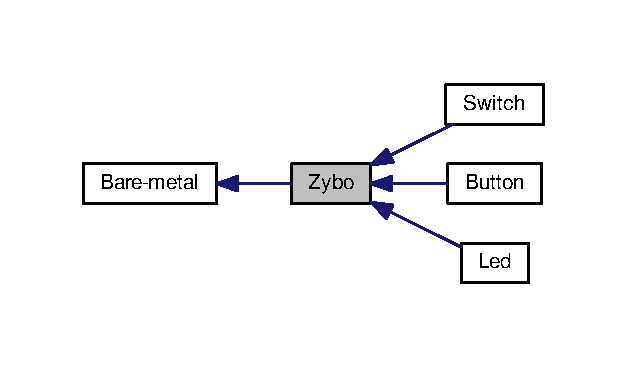
\includegraphics[width=201pt]{group___zybo}
\end{center}
\end{figure}
\subsection*{Moduli}
\begin{DoxyCompactItemize}
\item 
\hyperlink{group___button}{Button}
\item 
\hyperlink{group___led}{Led}
\item 
\hyperlink{group___switch}{Switch}
\end{DoxyCompactItemize}


\subsection{Descrizione dettagliata}

\hypertarget{group___button}{\section{Button}
\label{group___button}\index{Button@{Button}}
}
Diagramma di collaborazione per Button\+:\nopagebreak
\begin{figure}[H]
\begin{center}
\leavevmode
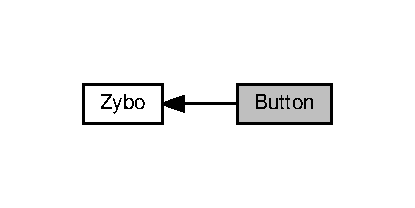
\includegraphics[width=199pt]{group___button}
\end{center}
\end{figure}
\subsection*{Strutture dati}
\begin{DoxyCompactItemize}
\item 
struct \hyperlink{struct_zybo_button__t}{Zybo\+Button\+\_\+t}
\begin{DoxyCompactList}\small\item\em Struttura opaca che astrae l'insieme dei button presenti sulla board Digilent Zybo;. \end{DoxyCompactList}\end{DoxyCompactItemize}
\subsection*{Definizioni}
\begin{DoxyCompactItemize}
\item 
\#define \hyperlink{group___button_ga5f85cbc14732f1d83faa75500b67defa}{Zybo\+Button}(i)~((uint32\+\_\+t)(1$<$$<$i))
\begin{DoxyCompactList}\small\item\em Metodo alternativo per la specifica di uno dei button presenti sulla board Digilent Zybo. \end{DoxyCompactList}\item 
\#define \hyperlink{group___button_ga8960eefa6a431f50d4fe2a2f8063da3f}{Zybo\+Button\+\_\+\+Debounce\+Wait}~50
\begin{DoxyCompactList}\small\item\em Tempo di attesa (in millisecondi) usato per prevenire il fenomeno del bouncing. Il valore di default è 50, determinato empiricamente. Puo' essere modificato a piacimento cambiando il valore alla macro seguente. \end{DoxyCompactList}\end{DoxyCompactItemize}
\subsection*{Tipi enumerati (enum)}
\begin{DoxyCompactItemize}
\item 
enum \hyperlink{group___button_ga4d26a5f6cad606de534ba034e0ba42dd}{Zybo\+Button\+\_\+mask\+\_\+t} \{ \hyperlink{group___button_gga4d26a5f6cad606de534ba034e0ba42ddaabede392be8cae14b8a070a804c754e8}{Zybo\+Button3} = 0x8, 
\hyperlink{group___button_gga4d26a5f6cad606de534ba034e0ba42dda2aa888c8f01ac8a79013e5ebc9eef609}{Zybo\+Button2} = 0x4, 
\hyperlink{group___button_gga4d26a5f6cad606de534ba034e0ba42dda29c35ef3133898c050f675a60de66dd7}{Zybo\+Button1} = 0x2, 
\hyperlink{group___button_gga4d26a5f6cad606de534ba034e0ba42dda2f821ce9661687aefb0ec4de65911570}{Zybo\+Button0} = 0x1
 \}
\begin{DoxyCompactList}\small\item\em Maschere di selezione dei Push\+Button. \end{DoxyCompactList}\item 
enum \hyperlink{group___button_ga85c290bfa232cab213e69200bf78e06a}{Zybo\+Button\+\_\+status\+\_\+t} \{ \hyperlink{group___button_gga85c290bfa232cab213e69200bf78e06aacd110f28912806bcec929721e8737399}{Zybo\+Button\+\_\+off}, 
\hyperlink{group___button_gga85c290bfa232cab213e69200bf78e06aa49bf4a6902270f28bc6a1146fbd1b1fe}{Zybo\+Button\+\_\+on}
 \}
\begin{DoxyCompactList}\small\item\em Status di attivo/inattivo dei Push\+Button. \end{DoxyCompactList}\end{DoxyCompactItemize}
\subsection*{Funzioni}
\begin{DoxyCompactItemize}
\item 
void \hyperlink{group___button_gaa40462223af93b0f5bdf2932400fe2a5}{Zybo\+Button\+\_\+init} (\hyperlink{struct_zybo_button__t}{Zybo\+Button\+\_\+t} $\ast$buttons, \hyperlink{struct_g_p_i_o__t}{G\+P\+I\+O\+\_\+t} $\ast$gpio, \hyperlink{group___g_p_i_o_ga6d5aef8a8a54ee2f602d47252ff66595}{G\+P\+I\+O\+\_\+mask} Button3\+\_\+pin, \hyperlink{group___g_p_i_o_ga6d5aef8a8a54ee2f602d47252ff66595}{G\+P\+I\+O\+\_\+mask} Button2\+\_\+pin, \hyperlink{group___g_p_i_o_ga6d5aef8a8a54ee2f602d47252ff66595}{G\+P\+I\+O\+\_\+mask} Button1\+\_\+pin, \hyperlink{group___g_p_i_o_ga6d5aef8a8a54ee2f602d47252ff66595}{G\+P\+I\+O\+\_\+mask} Button0\+\_\+pin)
\begin{DoxyCompactList}\small\item\em Inizializza un oggetto di tipo \hyperlink{struct_zybo_button__t}{Zybo\+Button\+\_\+t}. \end{DoxyCompactList}\item 
void \hyperlink{group___button_gaca30e81084e746785e395f79e9678e9a}{Zybo\+Button\+\_\+wait\+While\+Idle} (\hyperlink{struct_zybo_button__t}{Zybo\+Button\+\_\+t} $\ast$buttons)
\begin{DoxyCompactList}\small\item\em Permettere di mettere il programma in attesa attiva finche' i button restano inattivi;. \end{DoxyCompactList}\item 
void \hyperlink{group___button_ga3840edf011b5bad6302b7efc9c6326fe}{Zybo\+Button\+\_\+wait\+While\+Busy} (\hyperlink{struct_zybo_button__t}{Zybo\+Button\+\_\+t} $\ast$buttons)
\begin{DoxyCompactList}\small\item\em Permettere di mettere il programma in attesa attiva finche' i button restano attivi;. \end{DoxyCompactList}\item 
\hyperlink{group___button_ga85c290bfa232cab213e69200bf78e06a}{Zybo\+Button\+\_\+status\+\_\+t} \hyperlink{group___button_ga75407539e8ba0ad3ea142496219cd083}{Zybo\+Button\+\_\+get\+Status} (\hyperlink{struct_zybo_button__t}{Zybo\+Button\+\_\+t} $\ast$buttons, \hyperlink{group___button_ga4d26a5f6cad606de534ba034e0ba42dd}{Zybo\+Button\+\_\+mask\+\_\+t} mask)
\begin{DoxyCompactList}\small\item\em Permette la lettura dello stato dei button presenti sulla board. \end{DoxyCompactList}\end{DoxyCompactItemize}


\subsection{Descrizione dettagliata}


\subsection{Documentazione delle definizioni}
\hypertarget{group___button_ga5f85cbc14732f1d83faa75500b67defa}{\index{Button@{Button}!Zybo\+Button@{Zybo\+Button}}
\index{Zybo\+Button@{Zybo\+Button}!Button@{Button}}
\subsubsection[{Zybo\+Button}]{\setlength{\rightskip}{0pt plus 5cm}\#define Zybo\+Button(
\begin{DoxyParamCaption}
\item[{}]{i}
\end{DoxyParamCaption}
)~((uint32\+\_\+t)(1$<$$<$i))}}\label{group___button_ga5f85cbc14732f1d83faa75500b67defa}


Metodo alternativo per la specifica di uno dei button presenti sulla board Digilent Zybo. 


\begin{DoxyParams}{Parametri}
{\em i} & indice del button da selezionare, da 0 a 3 \\
\hline
\end{DoxyParams}
\begin{DoxyReturn}{Restituisce}
maschera di selezione del button i-\/esimo 
\end{DoxyReturn}
\hypertarget{group___button_ga8960eefa6a431f50d4fe2a2f8063da3f}{\index{Button@{Button}!Zybo\+Button\+\_\+\+Debounce\+Wait@{Zybo\+Button\+\_\+\+Debounce\+Wait}}
\index{Zybo\+Button\+\_\+\+Debounce\+Wait@{Zybo\+Button\+\_\+\+Debounce\+Wait}!Button@{Button}}
\subsubsection[{Zybo\+Button\+\_\+\+Debounce\+Wait}]{\setlength{\rightskip}{0pt plus 5cm}\#define Zybo\+Button\+\_\+\+Debounce\+Wait~50}}\label{group___button_ga8960eefa6a431f50d4fe2a2f8063da3f}


Tempo di attesa (in millisecondi) usato per prevenire il fenomeno del bouncing. Il valore di default è 50, determinato empiricamente. Puo' essere modificato a piacimento cambiando il valore alla macro seguente. 



\subsection{Documentazione dei tipi enumerati}
\hypertarget{group___button_ga4d26a5f6cad606de534ba034e0ba42dd}{\index{Button@{Button}!Zybo\+Button\+\_\+mask\+\_\+t@{Zybo\+Button\+\_\+mask\+\_\+t}}
\index{Zybo\+Button\+\_\+mask\+\_\+t@{Zybo\+Button\+\_\+mask\+\_\+t}!Button@{Button}}
\subsubsection[{Zybo\+Button\+\_\+mask\+\_\+t}]{\setlength{\rightskip}{0pt plus 5cm}enum {\bf Zybo\+Button\+\_\+mask\+\_\+t}}}\label{group___button_ga4d26a5f6cad606de534ba034e0ba42dd}


Maschere di selezione dei Push\+Button. 

\begin{Desc}
\item[Valori del tipo enumerato]\par
\begin{description}
\index{Zybo\+Button3@{Zybo\+Button3}!Button@{Button}}\index{Button@{Button}!Zybo\+Button3@{Zybo\+Button3}}\item[{\em 
\hypertarget{group___button_gga4d26a5f6cad606de534ba034e0ba42ddaabede392be8cae14b8a070a804c754e8}{Zybo\+Button3}\label{group___button_gga4d26a5f6cad606de534ba034e0ba42ddaabede392be8cae14b8a070a804c754e8}
}]Zybo\+Button3, seleziona il button 3 sulla board Digilent Zybo;. \index{Zybo\+Button2@{Zybo\+Button2}!Button@{Button}}\index{Button@{Button}!Zybo\+Button2@{Zybo\+Button2}}\item[{\em 
\hypertarget{group___button_gga4d26a5f6cad606de534ba034e0ba42dda2aa888c8f01ac8a79013e5ebc9eef609}{Zybo\+Button2}\label{group___button_gga4d26a5f6cad606de534ba034e0ba42dda2aa888c8f01ac8a79013e5ebc9eef609}
}]Zybo\+Button2, seleziona il button 2 sulla board Digilent Zybo;. \index{Zybo\+Button1@{Zybo\+Button1}!Button@{Button}}\index{Button@{Button}!Zybo\+Button1@{Zybo\+Button1}}\item[{\em 
\hypertarget{group___button_gga4d26a5f6cad606de534ba034e0ba42dda29c35ef3133898c050f675a60de66dd7}{Zybo\+Button1}\label{group___button_gga4d26a5f6cad606de534ba034e0ba42dda29c35ef3133898c050f675a60de66dd7}
}]Zybo\+Button1, seleziona il button 1 sulla board Digilent Zybo;. \index{Zybo\+Button0@{Zybo\+Button0}!Button@{Button}}\index{Button@{Button}!Zybo\+Button0@{Zybo\+Button0}}\item[{\em 
\hypertarget{group___button_gga4d26a5f6cad606de534ba034e0ba42dda2f821ce9661687aefb0ec4de65911570}{Zybo\+Button0}\label{group___button_gga4d26a5f6cad606de534ba034e0ba42dda2f821ce9661687aefb0ec4de65911570}
}]Zybo\+Button0, seleziona il button 0 sulla board Digilent Zybo;. \end{description}
\end{Desc}
\hypertarget{group___button_ga85c290bfa232cab213e69200bf78e06a}{\index{Button@{Button}!Zybo\+Button\+\_\+status\+\_\+t@{Zybo\+Button\+\_\+status\+\_\+t}}
\index{Zybo\+Button\+\_\+status\+\_\+t@{Zybo\+Button\+\_\+status\+\_\+t}!Button@{Button}}
\subsubsection[{Zybo\+Button\+\_\+status\+\_\+t}]{\setlength{\rightskip}{0pt plus 5cm}enum {\bf Zybo\+Button\+\_\+status\+\_\+t}}}\label{group___button_ga85c290bfa232cab213e69200bf78e06a}


Status di attivo/inattivo dei Push\+Button. 

\begin{Desc}
\item[Valori del tipo enumerato]\par
\begin{description}
\index{Zybo\+Button\+\_\+off@{Zybo\+Button\+\_\+off}!Button@{Button}}\index{Button@{Button}!Zybo\+Button\+\_\+off@{Zybo\+Button\+\_\+off}}\item[{\em 
\hypertarget{group___button_gga85c290bfa232cab213e69200bf78e06aacd110f28912806bcec929721e8737399}{Zybo\+Button\+\_\+off}\label{group___button_gga85c290bfa232cab213e69200bf78e06aacd110f28912806bcec929721e8737399}
}]Zybo\+Button\+\_\+off, corrisponde al valore logico '0', indica che un pushbutton e' inattivo;. \index{Zybo\+Button\+\_\+on@{Zybo\+Button\+\_\+on}!Button@{Button}}\index{Button@{Button}!Zybo\+Button\+\_\+on@{Zybo\+Button\+\_\+on}}\item[{\em 
\hypertarget{group___button_gga85c290bfa232cab213e69200bf78e06aa49bf4a6902270f28bc6a1146fbd1b1fe}{Zybo\+Button\+\_\+on}\label{group___button_gga85c290bfa232cab213e69200bf78e06aa49bf4a6902270f28bc6a1146fbd1b1fe}
}]Zybo\+Button\+\_\+on, corrisponde al valore logico '1', indica che un pushbutton e' attivo;. \end{description}
\end{Desc}


\subsection{Documentazione delle funzioni}
\hypertarget{group___button_ga75407539e8ba0ad3ea142496219cd083}{\index{Button@{Button}!Zybo\+Button\+\_\+get\+Status@{Zybo\+Button\+\_\+get\+Status}}
\index{Zybo\+Button\+\_\+get\+Status@{Zybo\+Button\+\_\+get\+Status}!Button@{Button}}
\subsubsection[{Zybo\+Button\+\_\+get\+Status}]{\setlength{\rightskip}{0pt plus 5cm}{\bf Zybo\+Button\+\_\+status\+\_\+t} Zybo\+Button\+\_\+get\+Status (
\begin{DoxyParamCaption}
\item[{{\bf Zybo\+Button\+\_\+t} $\ast$}]{buttons, }
\item[{{\bf Zybo\+Button\+\_\+mask\+\_\+t}}]{mask}
\end{DoxyParamCaption}
)}}\label{group___button_ga75407539e8ba0ad3ea142496219cd083}


Permette la lettura dello stato dei button presenti sulla board. 


\begin{DoxyParams}[1]{Parametri}
\mbox{\tt in}  & {\em buttons} & puntatore a struttura \hyperlink{struct_zybo_button__t}{Zybo\+Button\+\_\+t}, che astrae l'insieme dei button presenti sulla board Digilent Zybo; \\
\hline
\mbox{\tt in}  & {\em mask} & maschera di selezione dei button, quelli non selezionati non vengono tenuti in considerazione\\
\hline
\end{DoxyParams}
\begin{DoxyReturn}{Restituisce}
status status dei button 
\end{DoxyReturn}

\begin{DoxyRetVals}{Valori di ritorno}
{\em Zybo\+Button\+\_\+on} & se uno dei button selezionati e' attivo; \\
\hline
{\em Zybo\+Button\+\_\+off} & altrimenti\\
\hline
\end{DoxyRetVals}

\begin{DoxyCode}
1 ZyboButton\_status\_t button\_status = ZyboButton\_getStatus(&buttons, ZyboButton3);                // leggo lo
       stato ddi button 3
2 ZyboLed\_status\_t led\_status = (button\_status == ZyboButton\_on ? ZyboLed\_on : ZyboLed\_off);  // se lo stato
       e' attivo accendo il led 3
3 ZyboLed\_setStatus(&leds, ZyboLed3, led\_status);                                             //
       accendo/spengo led 3
\end{DoxyCode}


\begin{DoxyWarning}{Avvertimento}
Usa la macro assert per verificare che\+:
\begin{DoxyItemize}
\item buttons non sia un puntatore nullo;
\item buttons-\/$>$gpio non sia un puntatore nullo 
\end{DoxyItemize}
\end{DoxyWarning}
\hypertarget{group___button_gaa40462223af93b0f5bdf2932400fe2a5}{\index{Button@{Button}!Zybo\+Button\+\_\+init@{Zybo\+Button\+\_\+init}}
\index{Zybo\+Button\+\_\+init@{Zybo\+Button\+\_\+init}!Button@{Button}}
\subsubsection[{Zybo\+Button\+\_\+init}]{\setlength{\rightskip}{0pt plus 5cm}void Zybo\+Button\+\_\+init (
\begin{DoxyParamCaption}
\item[{{\bf Zybo\+Button\+\_\+t} $\ast$}]{buttons, }
\item[{{\bf G\+P\+I\+O\+\_\+t} $\ast$}]{gpio, }
\item[{{\bf G\+P\+I\+O\+\_\+mask}}]{Button3\+\_\+pin, }
\item[{{\bf G\+P\+I\+O\+\_\+mask}}]{Button2\+\_\+pin, }
\item[{{\bf G\+P\+I\+O\+\_\+mask}}]{Button1\+\_\+pin, }
\item[{{\bf G\+P\+I\+O\+\_\+mask}}]{Button0\+\_\+pin}
\end{DoxyParamCaption}
)}}\label{group___button_gaa40462223af93b0f5bdf2932400fe2a5}


Inizializza un oggetto di tipo \hyperlink{struct_zybo_button__t}{Zybo\+Button\+\_\+t}. 


\begin{DoxyParams}[1]{Parametri}
\mbox{\tt in,out}  & {\em buttons} & puntatore a struttura \hyperlink{struct_zybo_button__t}{Zybo\+Button\+\_\+t}, che astrae l'insieme dei button presenti sulla board Digilent Zybo; \\
\hline
\mbox{\tt in}  & {\em gpio} & puntatore a struttura \hyperlink{struct_g_p_i_o__t}{G\+P\+I\+O\+\_\+t}, che astrae un device G\+P\+I\+O; non viene inizializzato dalla funziona, sara' necessario inizializzarlo preventivamente; si faccia riferimento all'esempio riportato di seguito \\
\hline
\mbox{\tt in}  & {\em Button3\+\_\+pin} & pin del device G\+P\+I\+O a cui e' associato il button 3 della board Digilent Zybo; \\
\hline
\mbox{\tt in}  & {\em Button2\+\_\+pin} & pin del device G\+P\+I\+O a cui e' associato il button 2 della board Digilent Zybo; \\
\hline
\mbox{\tt in}  & {\em Button1\+\_\+pin} & pin del device G\+P\+I\+O a cui e' associato il button 1 della board Digilent Zybo; \\
\hline
\mbox{\tt in}  & {\em Button0\+\_\+pin} & pin del device G\+P\+I\+O a cui e' associato il button 0 della board Digilent Zybo;\\
\hline
\end{DoxyParams}

\begin{DoxyCode}
1 GPIO\_t gpioButton;
2 GPIO\_init(&gpioButton, XPAR\_MYGPIO\_1\_S00\_AXI\_BASEADDR, 4, 0, 4, 8);
3 ZyboButton\_t buttons;
4 ZyboButton\_init(&buttons, &gpioButton, GPIO\_pin3, GPIO\_pin2, GPIO\_pin1, GPIO\_pin0);
\end{DoxyCode}


\begin{DoxyWarning}{Avvertimento}
Usa la macro assert per verificare che\+:
\begin{DoxyItemize}
\item buttons non sia un puntatore nullo;
\item gpio non sia un puntatore nullo
\item Button\+N\+\_\+pin siano tutti pin differenti 
\end{DoxyItemize}
\end{DoxyWarning}
\hypertarget{group___button_ga3840edf011b5bad6302b7efc9c6326fe}{\index{Button@{Button}!Zybo\+Button\+\_\+wait\+While\+Busy@{Zybo\+Button\+\_\+wait\+While\+Busy}}
\index{Zybo\+Button\+\_\+wait\+While\+Busy@{Zybo\+Button\+\_\+wait\+While\+Busy}!Button@{Button}}
\subsubsection[{Zybo\+Button\+\_\+wait\+While\+Busy}]{\setlength{\rightskip}{0pt plus 5cm}void Zybo\+Button\+\_\+wait\+While\+Busy (
\begin{DoxyParamCaption}
\item[{{\bf Zybo\+Button\+\_\+t} $\ast$}]{buttons}
\end{DoxyParamCaption}
)}}\label{group___button_ga3840edf011b5bad6302b7efc9c6326fe}


Permettere di mettere il programma in attesa attiva finche' i button restano attivi;. 

\begin{DoxyWarning}{Avvertimento}
La funzione integra le funzionalita' di debouncing. Il tempo di attesa e' determinato sulla base del valore della macro Zybo\+Button\+\_\+\+Debounce\+Wait. Per l'attesa viene usata la funzione usleep() di stdlib.
\end{DoxyWarning}

\begin{DoxyParams}[1]{Parametri}
\mbox{\tt in}  & {\em buttons} & puntatore a struttura \hyperlink{struct_zybo_button__t}{Zybo\+Button\+\_\+t}, che astrae l'insieme dei button presenti sulla board Digilent Zybo;\\
\hline
\end{DoxyParams}

\begin{DoxyCode}
1 ZyboButton\_waitWhileIdle(&buttons);
2 ZyboButton\_status\_t button3\_status = ZyboButton\_getStatus(&buttons, ZyboButton3);               // leggo lo
       stato ddi button 3
3 ZyboButton\_status\_t button2\_status = ZyboButton\_getStatus(&buttons, ZyboButton2);               // leggo lo
       stato ddi button 2
4 ZyboButton\_status\_t button1\_status = ZyboButton\_getStatus(&buttons, ZyboButton1);               // leggo lo
       stato ddi button 1
5 ZyboButton\_status\_t button0\_status = ZyboButton\_getStatus(&buttons, ZyboButton0);               // leggo lo
       stato ddi button 0
6 ZyboButton\_waitWhileBusy(&buttons);
\end{DoxyCode}


\begin{DoxyWarning}{Avvertimento}
Usa la macro assert per verificare che\+:
\begin{DoxyItemize}
\item buttons non sia un puntatore nullo;
\item buttons-\/$>$gpio non sia un puntatore nullo 
\end{DoxyItemize}
\end{DoxyWarning}
\hypertarget{group___button_gaca30e81084e746785e395f79e9678e9a}{\index{Button@{Button}!Zybo\+Button\+\_\+wait\+While\+Idle@{Zybo\+Button\+\_\+wait\+While\+Idle}}
\index{Zybo\+Button\+\_\+wait\+While\+Idle@{Zybo\+Button\+\_\+wait\+While\+Idle}!Button@{Button}}
\subsubsection[{Zybo\+Button\+\_\+wait\+While\+Idle}]{\setlength{\rightskip}{0pt plus 5cm}void Zybo\+Button\+\_\+wait\+While\+Idle (
\begin{DoxyParamCaption}
\item[{{\bf Zybo\+Button\+\_\+t} $\ast$}]{buttons}
\end{DoxyParamCaption}
)}}\label{group___button_gaca30e81084e746785e395f79e9678e9a}


Permettere di mettere il programma in attesa attiva finche' i button restano inattivi;. 

\begin{DoxyWarning}{Avvertimento}
La funzione integra le funzionalita' di debouncing. Il tempo di attesa e' determinato sulla base del valore della macro Zybo\+Button\+\_\+\+Debounce\+Wait. Per l'attesa viene usata la funzione usleep() di stdlib.
\end{DoxyWarning}

\begin{DoxyParams}[1]{Parametri}
\mbox{\tt in}  & {\em buttons} & puntatore a struttura \hyperlink{struct_zybo_button__t}{Zybo\+Button\+\_\+t}, che astrae l'insieme dei button presenti sulla board Digilent Zybo;\\
\hline
\end{DoxyParams}

\begin{DoxyCode}
1 ZyboButton\_waitWhileIdle(&buttons);
2 ZyboButton\_status\_t button3\_status = ZyboButton\_getStatus(&buttons, ZyboButton3);               // leggo lo
       stato ddi button 3
3 ZyboButton\_status\_t button2\_status = ZyboButton\_getStatus(&buttons, ZyboButton2);               // leggo lo
       stato ddi button 2
4 ZyboButton\_status\_t button1\_status = ZyboButton\_getStatus(&buttons, ZyboButton1);               // leggo lo
       stato ddi button 1
5 ZyboButton\_status\_t button0\_status = ZyboButton\_getStatus(&buttons, ZyboButton0);               // leggo lo
       stato ddi button 0
6 ZyboButton\_waitWhileBusy(&buttons);
\end{DoxyCode}


\begin{DoxyWarning}{Avvertimento}
Usa la macro assert per verificare che\+:
\begin{DoxyItemize}
\item buttons non sia un puntatore nullo;
\item buttons-\/$>$gpio non sia un puntatore nullo 
\end{DoxyItemize}
\end{DoxyWarning}

\hypertarget{group___led}{\section{Led}
\label{group___led}\index{Led@{Led}}
}
Diagramma di collaborazione per Led\+:\nopagebreak
\begin{figure}[H]
\begin{center}
\leavevmode
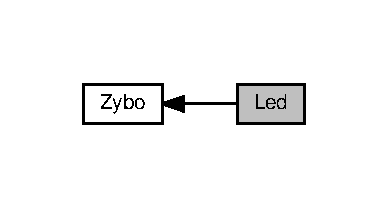
\includegraphics[width=186pt]{group___led}
\end{center}
\end{figure}
\subsection*{Strutture dati}
\begin{DoxyCompactItemize}
\item 
struct \hyperlink{struct_zybo_led__t}{Zybo\+Led\+\_\+t}
\begin{DoxyCompactList}\small\item\em Struttura opaca che astrae l'insieme dei Led presenti sulla board Digilent Zybo;. \end{DoxyCompactList}\end{DoxyCompactItemize}
\subsection*{Definizioni}
\begin{DoxyCompactItemize}
\item 
\#define \hyperlink{group___led_ga50ab39fed34dc3aaf53cdfd67d8ba25d}{Zybo\+Led}(i)~((uint32\+\_\+t)(1$<$$<$(i)))
\begin{DoxyCompactList}\small\item\em Metodo alternativo per la specifica di uno dei led presenti sulla board Digilent Zybo. \end{DoxyCompactList}\end{DoxyCompactItemize}
\subsection*{Tipi enumerati (enum)}
\begin{DoxyCompactItemize}
\item 
enum \hyperlink{group___led_gad11701cccac394f7e1f90de8f85695f3}{Zybo\+Led\+\_\+mask\+\_\+t} \{ \hyperlink{group___led_ggad11701cccac394f7e1f90de8f85695f3adc5edc2adfd899da9f149cb61364b141}{Zybo\+Led3} = 0x8\+U, 
\hyperlink{group___led_ggad11701cccac394f7e1f90de8f85695f3a4fa521f6fce7c4ba77d1d8144e71cdfc}{Zybo\+Led2} = 0x4\+U, 
\hyperlink{group___led_ggad11701cccac394f7e1f90de8f85695f3ad71c06f65dfffcf825d48f287718d9be}{Zybo\+Led1} = 0x2\+U, 
\hyperlink{group___led_ggad11701cccac394f7e1f90de8f85695f3ae1a1e8fa0bf803793ff27004884b85fe}{Zybo\+Led0} = 0x1\+U
 \}
\begin{DoxyCompactList}\small\item\em Maschere di selezione dei led. \end{DoxyCompactList}\item 
enum \hyperlink{group___led_ga3dcb274f22e577705c49944b8d1f4b12}{Zybo\+Led\+\_\+status\+\_\+t} \{ \hyperlink{group___led_gga3dcb274f22e577705c49944b8d1f4b12a9679f1c302afdb51915a2331b4ec92f3}{Zybo\+Led\+\_\+off}, 
\hyperlink{group___led_gga3dcb274f22e577705c49944b8d1f4b12aafcf0ae16a6edec807c06bb0a99f7e8b}{Zybo\+Led\+\_\+on}
 \}
\begin{DoxyCompactList}\small\item\em Status di accensione/spegnimento dei led. \end{DoxyCompactList}\end{DoxyCompactItemize}
\subsection*{Funzioni}
\begin{DoxyCompactItemize}
\item 
void \hyperlink{group___led_ga51bccd37e6ae8cd32e2c50c60a5e83cc}{Zybo\+Led\+\_\+init} (\hyperlink{struct_zybo_led__t}{Zybo\+Led\+\_\+t} $\ast$leds, \hyperlink{structmy_g_p_i_o__t}{my\+G\+P\+I\+O\+\_\+t} $\ast$gpio, \hyperlink{group__my_g_p_i_o_ga402a0d20afc0cb7c25554b8b023f4253}{my\+G\+P\+I\+O\+\_\+mask} Led3\+\_\+pin, \hyperlink{group__my_g_p_i_o_ga402a0d20afc0cb7c25554b8b023f4253}{my\+G\+P\+I\+O\+\_\+mask} Led2\+\_\+pin, \hyperlink{group__my_g_p_i_o_ga402a0d20afc0cb7c25554b8b023f4253}{my\+G\+P\+I\+O\+\_\+mask} Led1\+\_\+pin, \hyperlink{group__my_g_p_i_o_ga402a0d20afc0cb7c25554b8b023f4253}{my\+G\+P\+I\+O\+\_\+mask} Led0\+\_\+pin)
\begin{DoxyCompactList}\small\item\em Inizializza un oggetto di tipo \hyperlink{struct_zybo_led__t}{Zybo\+Led\+\_\+t}. \end{DoxyCompactList}\item 
void \hyperlink{group___led_gacf5c2b0328c4bdf2d796397fc4510c69}{Zybo\+Led\+\_\+set\+Status} (\hyperlink{struct_zybo_led__t}{Zybo\+Led\+\_\+t} $\ast$leds, \hyperlink{group___led_gad11701cccac394f7e1f90de8f85695f3}{Zybo\+Led\+\_\+mask\+\_\+t} mask, \hyperlink{group___led_ga3dcb274f22e577705c49944b8d1f4b12}{Zybo\+Led\+\_\+status\+\_\+t} status)
\begin{DoxyCompactList}\small\item\em Permette di accendere/spegnere i Led sulla board. \end{DoxyCompactList}\item 
void \hyperlink{group___led_ga20ddd78a98b4c0123c5b964aa0a59046}{Zybo\+Led\+\_\+toggle} (\hyperlink{struct_zybo_led__t}{Zybo\+Led\+\_\+t} $\ast$leds, \hyperlink{group___led_gad11701cccac394f7e1f90de8f85695f3}{Zybo\+Led\+\_\+mask\+\_\+t} mask)
\begin{DoxyCompactList}\small\item\em Permette di accendere/spegnere i Led sulla board, invertendone il valore. \end{DoxyCompactList}\end{DoxyCompactItemize}


\subsection{Descrizione dettagliata}


\subsection{Documentazione delle definizioni}
\hypertarget{group___led_ga50ab39fed34dc3aaf53cdfd67d8ba25d}{\index{Led@{Led}!Zybo\+Led@{Zybo\+Led}}
\index{Zybo\+Led@{Zybo\+Led}!Led@{Led}}
\subsubsection[{Zybo\+Led}]{\setlength{\rightskip}{0pt plus 5cm}\#define Zybo\+Led(
\begin{DoxyParamCaption}
\item[{}]{i}
\end{DoxyParamCaption}
)~((uint32\+\_\+t)(1$<$$<$(i)))}}\label{group___led_ga50ab39fed34dc3aaf53cdfd67d8ba25d}


Metodo alternativo per la specifica di uno dei led presenti sulla board Digilent Zybo. 


\begin{DoxyParams}[1]{Parametri}
\mbox{\tt in}  & {\em i} & indice del led da selezionare, da 0 a 3 \\
\hline
\end{DoxyParams}
\begin{DoxyReturn}{Restituisce}
maschera di selezione del led i-\/esimo 
\end{DoxyReturn}


\subsection{Documentazione dei tipi enumerati}
\hypertarget{group___led_gad11701cccac394f7e1f90de8f85695f3}{\index{Led@{Led}!Zybo\+Led\+\_\+mask\+\_\+t@{Zybo\+Led\+\_\+mask\+\_\+t}}
\index{Zybo\+Led\+\_\+mask\+\_\+t@{Zybo\+Led\+\_\+mask\+\_\+t}!Led@{Led}}
\subsubsection[{Zybo\+Led\+\_\+mask\+\_\+t}]{\setlength{\rightskip}{0pt plus 5cm}enum {\bf Zybo\+Led\+\_\+mask\+\_\+t}}}\label{group___led_gad11701cccac394f7e1f90de8f85695f3}


Maschere di selezione dei led. 

\begin{Desc}
\item[Valori del tipo enumerato]\par
\begin{description}
\index{Zybo\+Led3@{Zybo\+Led3}!Led@{Led}}\index{Led@{Led}!Zybo\+Led3@{Zybo\+Led3}}\item[{\em 
\hypertarget{group___led_ggad11701cccac394f7e1f90de8f85695f3adc5edc2adfd899da9f149cb61364b141}{Zybo\+Led3}\label{group___led_ggad11701cccac394f7e1f90de8f85695f3adc5edc2adfd899da9f149cb61364b141}
}]Zybo\+Led3, seleziona il led 3 sulla board Digilent Zybo;. \index{Zybo\+Led2@{Zybo\+Led2}!Led@{Led}}\index{Led@{Led}!Zybo\+Led2@{Zybo\+Led2}}\item[{\em 
\hypertarget{group___led_ggad11701cccac394f7e1f90de8f85695f3a4fa521f6fce7c4ba77d1d8144e71cdfc}{Zybo\+Led2}\label{group___led_ggad11701cccac394f7e1f90de8f85695f3a4fa521f6fce7c4ba77d1d8144e71cdfc}
}]Zybo\+Led2, seleziona il led 2 sulla board Digilent Zybo;. \index{Zybo\+Led1@{Zybo\+Led1}!Led@{Led}}\index{Led@{Led}!Zybo\+Led1@{Zybo\+Led1}}\item[{\em 
\hypertarget{group___led_ggad11701cccac394f7e1f90de8f85695f3ad71c06f65dfffcf825d48f287718d9be}{Zybo\+Led1}\label{group___led_ggad11701cccac394f7e1f90de8f85695f3ad71c06f65dfffcf825d48f287718d9be}
}]Zybo\+Led1, seleziona il led 1 sulla board Digilent Zybo;. \index{Zybo\+Led0@{Zybo\+Led0}!Led@{Led}}\index{Led@{Led}!Zybo\+Led0@{Zybo\+Led0}}\item[{\em 
\hypertarget{group___led_ggad11701cccac394f7e1f90de8f85695f3ae1a1e8fa0bf803793ff27004884b85fe}{Zybo\+Led0}\label{group___led_ggad11701cccac394f7e1f90de8f85695f3ae1a1e8fa0bf803793ff27004884b85fe}
}]Zybo\+Led0, seleziona il led 0 sulla board Digilent Zybo;. \end{description}
\end{Desc}
\hypertarget{group___led_ga3dcb274f22e577705c49944b8d1f4b12}{\index{Led@{Led}!Zybo\+Led\+\_\+status\+\_\+t@{Zybo\+Led\+\_\+status\+\_\+t}}
\index{Zybo\+Led\+\_\+status\+\_\+t@{Zybo\+Led\+\_\+status\+\_\+t}!Led@{Led}}
\subsubsection[{Zybo\+Led\+\_\+status\+\_\+t}]{\setlength{\rightskip}{0pt plus 5cm}enum {\bf Zybo\+Led\+\_\+status\+\_\+t}}}\label{group___led_ga3dcb274f22e577705c49944b8d1f4b12}


Status di accensione/spegnimento dei led. 

\begin{Desc}
\item[Valori del tipo enumerato]\par
\begin{description}
\index{Zybo\+Led\+\_\+off@{Zybo\+Led\+\_\+off}!Led@{Led}}\index{Led@{Led}!Zybo\+Led\+\_\+off@{Zybo\+Led\+\_\+off}}\item[{\em 
\hypertarget{group___led_gga3dcb274f22e577705c49944b8d1f4b12a9679f1c302afdb51915a2331b4ec92f3}{Zybo\+Led\+\_\+off}\label{group___led_gga3dcb274f22e577705c49944b8d1f4b12a9679f1c302afdb51915a2331b4ec92f3}
}]Zybo\+Led\+\_\+off, corrisponde al valore logico '0', per lo spegnimento dei Led. \index{Zybo\+Led\+\_\+on@{Zybo\+Led\+\_\+on}!Led@{Led}}\index{Led@{Led}!Zybo\+Led\+\_\+on@{Zybo\+Led\+\_\+on}}\item[{\em 
\hypertarget{group___led_gga3dcb274f22e577705c49944b8d1f4b12aafcf0ae16a6edec807c06bb0a99f7e8b}{Zybo\+Led\+\_\+on}\label{group___led_gga3dcb274f22e577705c49944b8d1f4b12aafcf0ae16a6edec807c06bb0a99f7e8b}
}]Zybo\+Led\+\_\+on, corrisponde al valore logico '1', per l'accensione dei Led. \end{description}
\end{Desc}


\subsection{Documentazione delle funzioni}
\hypertarget{group___led_ga51bccd37e6ae8cd32e2c50c60a5e83cc}{\index{Led@{Led}!Zybo\+Led\+\_\+init@{Zybo\+Led\+\_\+init}}
\index{Zybo\+Led\+\_\+init@{Zybo\+Led\+\_\+init}!Led@{Led}}
\subsubsection[{Zybo\+Led\+\_\+init}]{\setlength{\rightskip}{0pt plus 5cm}void Zybo\+Led\+\_\+init (
\begin{DoxyParamCaption}
\item[{{\bf Zybo\+Led\+\_\+t} $\ast$}]{leds, }
\item[{{\bf my\+G\+P\+I\+O\+\_\+t} $\ast$}]{gpio, }
\item[{{\bf my\+G\+P\+I\+O\+\_\+mask}}]{Led3\+\_\+pin, }
\item[{{\bf my\+G\+P\+I\+O\+\_\+mask}}]{Led2\+\_\+pin, }
\item[{{\bf my\+G\+P\+I\+O\+\_\+mask}}]{Led1\+\_\+pin, }
\item[{{\bf my\+G\+P\+I\+O\+\_\+mask}}]{Led0\+\_\+pin}
\end{DoxyParamCaption}
)}}\label{group___led_ga51bccd37e6ae8cd32e2c50c60a5e83cc}


Inizializza un oggetto di tipo \hyperlink{struct_zybo_led__t}{Zybo\+Led\+\_\+t}. 

Inizializza un oggetto di tipo \hyperlink{struct_zybo_led__t}{Zybo\+Led\+\_\+t}, che astrae e consente di pilotare i led presenti sulla board Digilent Zybo. Per il pilotaggio viene usato il modulo G\+P\+I\+O ed un puntatore ad una struttura \hyperlink{structmy_g_p_i_o__t}{my\+G\+P\+I\+O\+\_\+t} che lo astrae. Tale struttura non viene inizializzata dalla funzione Zybo\+Led\+\_\+init, per cui sara' necessario inizializzarlo preventivamente. La funzione, pero', si assume l'onere di configurare i pin del device G\+P\+I\+O a cui i led sono connessi.


\begin{DoxyParams}[1]{Parametri}
\mbox{\tt in,out}  & {\em leds} & puntatore a struttura \hyperlink{struct_zybo_led__t}{Zybo\+Led\+\_\+t}, che astrae l'insieme dei Led presenti sulla board Digilent Zybo; \\
\hline
\mbox{\tt in}  & {\em gpio} & puntatore a struttura \hyperlink{structmy_g_p_i_o__t}{my\+G\+P\+I\+O\+\_\+t}, che astrae un device G\+P\+I\+O; la struttura \hyperlink{structmy_g_p_i_o__t}{my\+G\+P\+I\+O\+\_\+t} non viene inizializzata dalla funzione, per cui sara' necessario farlo preventivamente; si faccia riferimento all'esempio riportato di seguito. \\
\hline
\mbox{\tt in}  & {\em Led3\+\_\+pin} & pin del device G\+P\+I\+O a cui e' associato il Led3 della board Digilent Zybo; \\
\hline
\mbox{\tt in}  & {\em Led2\+\_\+pin} & pin del device G\+P\+I\+O a cui e' associato il Led2 della board Digilent Zybo; \\
\hline
\mbox{\tt in}  & {\em Led1\+\_\+pin} & pin del device G\+P\+I\+O a cui e' associato il Led1 della board Digilent Zybo; \\
\hline
\mbox{\tt in}  & {\em Led0\+\_\+pin} & pin del device G\+P\+I\+O a cui e' associato il Led0 della board Digilent Zybo;\\
\hline
\end{DoxyParams}

\begin{DoxyCode}
1 myGPIO\_t gpioLed;
2 GPIO\_init(&gpioLed, XPAR\_MYGPIO\_0\_S00\_AXI\_BASEADDR, 4, 0, 4, 8);                // inizializzazione del
       device GPIO
3 ZyboLed\_t leds;
4 ZyboLed\_init(&leds, &gpioLed, GPIO\_pin3, GPIO\_pin2, GPIO\_pin1, GPIO\_pin0);  // inzializzazione della
       struttura ZyboLed\_t
\end{DoxyCode}


\begin{DoxyWarning}{Avvertimento}
Usa la macro assert per verificare che\+:
\begin{DoxyItemize}
\item leds non sia un puntatore nullo;
\item gpio non sia un puntatore nullo
\item Led\+N\+\_\+pin siano tutti pin differenti 
\end{DoxyItemize}
\end{DoxyWarning}
\hypertarget{group___led_gacf5c2b0328c4bdf2d796397fc4510c69}{\index{Led@{Led}!Zybo\+Led\+\_\+set\+Status@{Zybo\+Led\+\_\+set\+Status}}
\index{Zybo\+Led\+\_\+set\+Status@{Zybo\+Led\+\_\+set\+Status}!Led@{Led}}
\subsubsection[{Zybo\+Led\+\_\+set\+Status}]{\setlength{\rightskip}{0pt plus 5cm}void Zybo\+Led\+\_\+set\+Status (
\begin{DoxyParamCaption}
\item[{{\bf Zybo\+Led\+\_\+t} $\ast$}]{leds, }
\item[{{\bf Zybo\+Led\+\_\+mask\+\_\+t}}]{mask, }
\item[{{\bf Zybo\+Led\+\_\+status\+\_\+t}}]{status}
\end{DoxyParamCaption}
)}}\label{group___led_gacf5c2b0328c4bdf2d796397fc4510c69}


Permette di accendere/spegnere i Led sulla board. 


\begin{DoxyParams}[1]{Parametri}
\mbox{\tt in}  & {\em leds} & puntatore a struttura \hyperlink{struct_zybo_led__t}{Zybo\+Led\+\_\+t}, che astrae l'insieme dei Led presenti sulla board Digilent Zybo; \\
\hline
\mbox{\tt in}  & {\em mask} & maschera di selezione dei led, quelli non selezionati vengono lasciati inalterati \\
\hline
\mbox{\tt in}  & {\em status} & status dei led, Zybo\+Led\+\_\+on per accendere, Zybo\+Led\+\_\+off per spegnere\\
\hline
\end{DoxyParams}

\begin{DoxyCode}
1 ZyboLed\_setStatus(&leds, ZyboLed3 | ZyboLed1, ZyboLed\_on);  // accensione dei Led 3 ed 1
2 ZyboLed\_setStatus(&leds, ZyboLed3 | ZyboLed1, ZyboLed\_off); // spegnimento dei Led 3 ed 1
3 ZyboLed\_setStatus(&leds, ZyboLed2 | ZyboLed0, ZyboLed\_on);  // accendsione dei Led 2 ed 0
4 ZyboLed\_setStatus(&leds, ZyboLed2 | ZyboLed0, ZyboLed\_off); // spegnimento dei Led 2 ed 0
5 ZyboLed\_setStatus(&leds, ZyboLed3 | ZyboLed1 | ZyboLed2 | ZyboLed0, ZyboLed\_on);        // accensone di
       tutti i led
6 ZyboLed\_setStatus(&leds, ZyboLed3 | ZyboLed1 | ZyboLed2 | ZyboLed0, ZyboLed\_off);   // spegnimento di tutti
       i led
\end{DoxyCode}


\begin{DoxyWarning}{Avvertimento}
Usa la macro assert per verificare che\+:
\begin{DoxyItemize}
\item leds non sia un puntatore nullo;
\item leds-\/$>$gpio non sia un puntatore nullo 
\end{DoxyItemize}
\end{DoxyWarning}
\hypertarget{group___led_ga20ddd78a98b4c0123c5b964aa0a59046}{\index{Led@{Led}!Zybo\+Led\+\_\+toggle@{Zybo\+Led\+\_\+toggle}}
\index{Zybo\+Led\+\_\+toggle@{Zybo\+Led\+\_\+toggle}!Led@{Led}}
\subsubsection[{Zybo\+Led\+\_\+toggle}]{\setlength{\rightskip}{0pt plus 5cm}void Zybo\+Led\+\_\+toggle (
\begin{DoxyParamCaption}
\item[{{\bf Zybo\+Led\+\_\+t} $\ast$}]{leds, }
\item[{{\bf Zybo\+Led\+\_\+mask\+\_\+t}}]{mask}
\end{DoxyParamCaption}
)}}\label{group___led_ga20ddd78a98b4c0123c5b964aa0a59046}


Permette di accendere/spegnere i Led sulla board, invertendone il valore. 


\begin{DoxyParams}[1]{Parametri}
\mbox{\tt in}  & {\em leds} & puntatore a struttura \hyperlink{struct_zybo_led__t}{Zybo\+Led\+\_\+t}, che astrae l'insieme dei Led presenti sulla board Digilent Zybo; \\
\hline
\mbox{\tt in}  & {\em mask} & maschera di selezione dei led, quelli non selezionati vengono lasciati inalterati\\
\hline
\end{DoxyParams}

\begin{DoxyCode}
1 ZyboLed\_toggle(&leds, ZyboLed3 | ZyboLed1); // accensione/spegnimento dei Led 3 ed 1
\end{DoxyCode}


\begin{DoxyWarning}{Avvertimento}
Usa la macro assert per verificare che\+:
\begin{DoxyItemize}
\item leds non sia un puntatore nullo;
\item leds-\/$>$gpio non sia un puntatore nullo 
\end{DoxyItemize}
\end{DoxyWarning}

\hypertarget{group___switch}{\section{Switch}
\label{group___switch}\index{Switch@{Switch}}
}
Diagramma di collaborazione per Switch\+:
\nopagebreak
\begin{figure}[H]
\begin{center}
\leavevmode
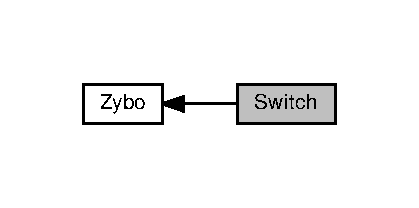
\includegraphics[width=201pt]{group___switch}
\end{center}
\end{figure}
\subsection*{Strutture dati}
\begin{DoxyCompactItemize}
\item 
struct \hyperlink{struct_zybo_switch__t}{Zybo\+Switch\+\_\+t}
\begin{DoxyCompactList}\small\item\em Struttura opaca che astrae l'insieme degli switch presenti sulla board Digilent Zybo;. \end{DoxyCompactList}\end{DoxyCompactItemize}
\subsection*{Definizioni}
\begin{DoxyCompactItemize}
\item 
\#define \hyperlink{group___switch_ga1c463f6e1e3a43f68109c176772ce5cc}{Zybo\+Switch}(i)~((uint32\+\_\+t)(1$<$$<$i))
\begin{DoxyCompactList}\small\item\em Metodo alternativo per la specifica di uno degli switch presenti sulla board Digilent Zybo. \end{DoxyCompactList}\end{DoxyCompactItemize}
\subsection*{Tipi enumerati (enum)}
\begin{DoxyCompactItemize}
\item 
enum \hyperlink{group___switch_ga2e0602a824354f25c395f938caba3703}{Zybo\+Switch\+\_\+mask\+\_\+t} \{ \hyperlink{group___switch_gga2e0602a824354f25c395f938caba3703a73ccea5ad8c919fe962e9a67a3733ee3}{Zybo\+Switch3} = 0x8, 
\hyperlink{group___switch_gga2e0602a824354f25c395f938caba3703aac2f5ebb28eb3bd93fcdf8019b6a3e9e}{Zybo\+Switch2} = 0x4, 
\hyperlink{group___switch_gga2e0602a824354f25c395f938caba3703a694a25c87b1ec597d2a6032bf5d34b0f}{Zybo\+Switch1} = 0x2, 
\hyperlink{group___switch_gga2e0602a824354f25c395f938caba3703a84350e8b6e7a7e2cabf22fc7a1a5c651}{Zybo\+Switch0} = 0x1
 \}
\begin{DoxyCompactList}\small\item\em Maschere di selezione degli switch. \end{DoxyCompactList}\item 
enum \hyperlink{group___switch_ga4ba6b49b2f47ebb464aefcea7e23e04a}{Zybo\+Switch\+\_\+status\+\_\+t} \{ \hyperlink{group___switch_gga4ba6b49b2f47ebb464aefcea7e23e04aa1d686faf83e8606e68eec0b7e525a755}{Zybo\+Switch\+\_\+off}, 
\hyperlink{group___switch_gga4ba6b49b2f47ebb464aefcea7e23e04aafba009508b8822de867af69034e3e4f8}{Zybo\+Switch\+\_\+on}
 \}
\begin{DoxyCompactList}\small\item\em Status di attivo/inattivo degli switch. \end{DoxyCompactList}\end{DoxyCompactItemize}
\subsection*{Funzioni}
\begin{DoxyCompactItemize}
\item 
void \hyperlink{group___switch_ga121018c0ccfeb05b6e8f692a5a6955d7}{Zybo\+Switch\+\_\+init} (\hyperlink{struct_zybo_switch__t}{Zybo\+Switch\+\_\+t} $\ast$switches, \hyperlink{struct_g_p_i_o__t}{G\+P\+I\+O\+\_\+t} $\ast$gpio, \hyperlink{group___g_p_i_o_ga6d5aef8a8a54ee2f602d47252ff66595}{G\+P\+I\+O\+\_\+mask} Switch3\+\_\+pin, \hyperlink{group___g_p_i_o_ga6d5aef8a8a54ee2f602d47252ff66595}{G\+P\+I\+O\+\_\+mask} Switch2\+\_\+pin, \hyperlink{group___g_p_i_o_ga6d5aef8a8a54ee2f602d47252ff66595}{G\+P\+I\+O\+\_\+mask} Switch1\+\_\+pin, \hyperlink{group___g_p_i_o_ga6d5aef8a8a54ee2f602d47252ff66595}{G\+P\+I\+O\+\_\+mask} Switch0\+\_\+pin)
\begin{DoxyCompactList}\small\item\em Inizializza un oggetto di tipo \hyperlink{struct_zybo_switch__t}{Zybo\+Switch\+\_\+t}. \end{DoxyCompactList}\item 
\hyperlink{group___switch_ga4ba6b49b2f47ebb464aefcea7e23e04a}{Zybo\+Switch\+\_\+status\+\_\+t} \hyperlink{group___switch_gafac8daf9a9a585f8f20ef2a6fa883a1f}{Zybo\+Switch\+\_\+get\+Status} (\hyperlink{struct_zybo_switch__t}{Zybo\+Switch\+\_\+t} $\ast$switches, \hyperlink{group___switch_ga2e0602a824354f25c395f938caba3703}{Zybo\+Switch\+\_\+mask\+\_\+t} mask)
\begin{DoxyCompactList}\small\item\em Permette la lettura dello stato degli switch presenti sulla board. \end{DoxyCompactList}\end{DoxyCompactItemize}


\subsection{Descrizione dettagliata}


\subsection{Documentazione delle definizioni}
\hypertarget{group___switch_ga1c463f6e1e3a43f68109c176772ce5cc}{\index{Switch@{Switch}!Zybo\+Switch@{Zybo\+Switch}}
\index{Zybo\+Switch@{Zybo\+Switch}!Switch@{Switch}}
\subsubsection[{Zybo\+Switch}]{\setlength{\rightskip}{0pt plus 5cm}\#define Zybo\+Switch(
\begin{DoxyParamCaption}
\item[{}]{i}
\end{DoxyParamCaption}
)~((uint32\+\_\+t)(1$<$$<$i))}}\label{group___switch_ga1c463f6e1e3a43f68109c176772ce5cc}


Metodo alternativo per la specifica di uno degli switch presenti sulla board Digilent Zybo. 


\begin{DoxyParams}{Parametri}
{\em i} & indice dello switch da selezionare, da 0 a 3 \\
\hline
\end{DoxyParams}
\begin{DoxyReturn}{Restituisce}
maschera di selezione dello switch i-\/esimo 
\end{DoxyReturn}


\subsection{Documentazione dei tipi enumerati}
\hypertarget{group___switch_ga2e0602a824354f25c395f938caba3703}{\index{Switch@{Switch}!Zybo\+Switch\+\_\+mask\+\_\+t@{Zybo\+Switch\+\_\+mask\+\_\+t}}
\index{Zybo\+Switch\+\_\+mask\+\_\+t@{Zybo\+Switch\+\_\+mask\+\_\+t}!Switch@{Switch}}
\subsubsection[{Zybo\+Switch\+\_\+mask\+\_\+t}]{\setlength{\rightskip}{0pt plus 5cm}enum {\bf Zybo\+Switch\+\_\+mask\+\_\+t}}}\label{group___switch_ga2e0602a824354f25c395f938caba3703}


Maschere di selezione degli switch. 

\begin{Desc}
\item[Valori del tipo enumerato]\par
\begin{description}
\index{Zybo\+Switch3@{Zybo\+Switch3}!Switch@{Switch}}\index{Switch@{Switch}!Zybo\+Switch3@{Zybo\+Switch3}}\item[{\em 
\hypertarget{group___switch_gga2e0602a824354f25c395f938caba3703a73ccea5ad8c919fe962e9a67a3733ee3}{Zybo\+Switch3}\label{group___switch_gga2e0602a824354f25c395f938caba3703a73ccea5ad8c919fe962e9a67a3733ee3}
}]Zybo\+Switch3, seleziona lo switch 3 sulla board Digilent Zybo;. \index{Zybo\+Switch2@{Zybo\+Switch2}!Switch@{Switch}}\index{Switch@{Switch}!Zybo\+Switch2@{Zybo\+Switch2}}\item[{\em 
\hypertarget{group___switch_gga2e0602a824354f25c395f938caba3703aac2f5ebb28eb3bd93fcdf8019b6a3e9e}{Zybo\+Switch2}\label{group___switch_gga2e0602a824354f25c395f938caba3703aac2f5ebb28eb3bd93fcdf8019b6a3e9e}
}]Zybo\+Switch2, seleziona lo switch 2 sulla board Digilent Zybo;. \index{Zybo\+Switch1@{Zybo\+Switch1}!Switch@{Switch}}\index{Switch@{Switch}!Zybo\+Switch1@{Zybo\+Switch1}}\item[{\em 
\hypertarget{group___switch_gga2e0602a824354f25c395f938caba3703a694a25c87b1ec597d2a6032bf5d34b0f}{Zybo\+Switch1}\label{group___switch_gga2e0602a824354f25c395f938caba3703a694a25c87b1ec597d2a6032bf5d34b0f}
}]Zybo\+Switch1, seleziona lo switch 1 sulla board Digilent Zybo;. \index{Zybo\+Switch0@{Zybo\+Switch0}!Switch@{Switch}}\index{Switch@{Switch}!Zybo\+Switch0@{Zybo\+Switch0}}\item[{\em 
\hypertarget{group___switch_gga2e0602a824354f25c395f938caba3703a84350e8b6e7a7e2cabf22fc7a1a5c651}{Zybo\+Switch0}\label{group___switch_gga2e0602a824354f25c395f938caba3703a84350e8b6e7a7e2cabf22fc7a1a5c651}
}]Zybo\+Switch0, seleziona lo switch 0 sulla board Digilent Zybo;. \end{description}
\end{Desc}
\hypertarget{group___switch_ga4ba6b49b2f47ebb464aefcea7e23e04a}{\index{Switch@{Switch}!Zybo\+Switch\+\_\+status\+\_\+t@{Zybo\+Switch\+\_\+status\+\_\+t}}
\index{Zybo\+Switch\+\_\+status\+\_\+t@{Zybo\+Switch\+\_\+status\+\_\+t}!Switch@{Switch}}
\subsubsection[{Zybo\+Switch\+\_\+status\+\_\+t}]{\setlength{\rightskip}{0pt plus 5cm}enum {\bf Zybo\+Switch\+\_\+status\+\_\+t}}}\label{group___switch_ga4ba6b49b2f47ebb464aefcea7e23e04a}


Status di attivo/inattivo degli switch. 

\begin{Desc}
\item[Valori del tipo enumerato]\par
\begin{description}
\index{Zybo\+Switch\+\_\+off@{Zybo\+Switch\+\_\+off}!Switch@{Switch}}\index{Switch@{Switch}!Zybo\+Switch\+\_\+off@{Zybo\+Switch\+\_\+off}}\item[{\em 
\hypertarget{group___switch_gga4ba6b49b2f47ebb464aefcea7e23e04aa1d686faf83e8606e68eec0b7e525a755}{Zybo\+Switch\+\_\+off}\label{group___switch_gga4ba6b49b2f47ebb464aefcea7e23e04aa1d686faf83e8606e68eec0b7e525a755}
}]Zybo\+Switch\+\_\+off, corrisponde al valore logico '0', indica che lo switch e' inattivo;. \index{Zybo\+Switch\+\_\+on@{Zybo\+Switch\+\_\+on}!Switch@{Switch}}\index{Switch@{Switch}!Zybo\+Switch\+\_\+on@{Zybo\+Switch\+\_\+on}}\item[{\em 
\hypertarget{group___switch_gga4ba6b49b2f47ebb464aefcea7e23e04aafba009508b8822de867af69034e3e4f8}{Zybo\+Switch\+\_\+on}\label{group___switch_gga4ba6b49b2f47ebb464aefcea7e23e04aafba009508b8822de867af69034e3e4f8}
}]Zybo\+Switch\+\_\+on, corrisponde al valore logico '1', indica che lo switch e' attivo;. \end{description}
\end{Desc}


\subsection{Documentazione delle funzioni}
\hypertarget{group___switch_gafac8daf9a9a585f8f20ef2a6fa883a1f}{\index{Switch@{Switch}!Zybo\+Switch\+\_\+get\+Status@{Zybo\+Switch\+\_\+get\+Status}}
\index{Zybo\+Switch\+\_\+get\+Status@{Zybo\+Switch\+\_\+get\+Status}!Switch@{Switch}}
\subsubsection[{Zybo\+Switch\+\_\+get\+Status}]{\setlength{\rightskip}{0pt plus 5cm}{\bf Zybo\+Switch\+\_\+status\+\_\+t} Zybo\+Switch\+\_\+get\+Status (
\begin{DoxyParamCaption}
\item[{{\bf Zybo\+Switch\+\_\+t} $\ast$}]{switches, }
\item[{{\bf Zybo\+Switch\+\_\+mask\+\_\+t}}]{mask}
\end{DoxyParamCaption}
)}}\label{group___switch_gafac8daf9a9a585f8f20ef2a6fa883a1f}


Permette la lettura dello stato degli switch presenti sulla board. 


\begin{DoxyParams}{Parametri}
{\em switches} & puntatore a struttura \hyperlink{struct_zybo_switch__t}{Zybo\+Switch\+\_\+t}, che astrae l'insieme degli switch presenti sulla board Digilent Zybo; \\
\hline
{\em mask} & maschera di selezione degli switch, quelli non selezionati non vengono tenuti in considerazione \\
\hline
\end{DoxyParams}
\begin{DoxyReturn}{Restituisce}
status status degli switch 
\end{DoxyReturn}

\begin{DoxyRetVals}{Valori di ritorno}
{\em Zybo\+Switch\+\_\+on} & se uno degli switch selezionati e' attivo; \\
\hline
{\em Zybo\+Switch\+\_\+off} & altrimenti\\
\hline
\end{DoxyRetVals}

\begin{DoxyCode}
1 ZyboSwitch\_status\_t switch\_status = ZyboSwitch\_getStatus(&switches, ZyboSwitch3);           // leggo lo
       stato dello switch 3
2 ZyboLed\_status\_t led\_status = (switch\_status == ZyboSwitch\_on ? ZyboLed\_on : ZyboLed\_off);  // se lo switch
       3 e' attivo accendo il led 3
3 ZyboLed\_setStatus(&leds, ZyboLed3, led\_status);                                             //
       accendo/spengo led 3
\end{DoxyCode}


\begin{DoxyWarning}{Avvertimento}
Usa la macro assert per verificare che\+:
\begin{DoxyItemize}
\item switches non sia un puntatore nullo;
\item switches-\/$>$gpio non sia un puntatore nullo 
\end{DoxyItemize}
\end{DoxyWarning}
\hypertarget{group___switch_ga121018c0ccfeb05b6e8f692a5a6955d7}{\index{Switch@{Switch}!Zybo\+Switch\+\_\+init@{Zybo\+Switch\+\_\+init}}
\index{Zybo\+Switch\+\_\+init@{Zybo\+Switch\+\_\+init}!Switch@{Switch}}
\subsubsection[{Zybo\+Switch\+\_\+init}]{\setlength{\rightskip}{0pt plus 5cm}void Zybo\+Switch\+\_\+init (
\begin{DoxyParamCaption}
\item[{{\bf Zybo\+Switch\+\_\+t} $\ast$}]{switches, }
\item[{{\bf G\+P\+I\+O\+\_\+t} $\ast$}]{gpio, }
\item[{{\bf G\+P\+I\+O\+\_\+mask}}]{Switch3\+\_\+pin, }
\item[{{\bf G\+P\+I\+O\+\_\+mask}}]{Switch2\+\_\+pin, }
\item[{{\bf G\+P\+I\+O\+\_\+mask}}]{Switch1\+\_\+pin, }
\item[{{\bf G\+P\+I\+O\+\_\+mask}}]{Switch0\+\_\+pin}
\end{DoxyParamCaption}
)}}\label{group___switch_ga121018c0ccfeb05b6e8f692a5a6955d7}


Inizializza un oggetto di tipo \hyperlink{struct_zybo_switch__t}{Zybo\+Switch\+\_\+t}. 


\begin{DoxyParams}{Parametri}
{\em switches} & puntatore a struttura \hyperlink{struct_zybo_switch__t}{Zybo\+Switch\+\_\+t}, che astrae l'insieme degli switch presenti sulla board Digilent Zybo; \\
\hline
{\em gpio} & puntatore a struttura \hyperlink{struct_g_p_i_o__t}{G\+P\+I\+O\+\_\+t}, che astrae un device G\+P\+I\+O; non viene inizializzato dalla funziona, sara' necessario inizializzarlo preventivamente; si faccia riferimento all'esempio riportato di seguito \\
\hline
{\em Switch3\+\_\+pin} & pin del device G\+P\+I\+O a cui e' associato lo switch 3 della board Digilent Zybo; \\
\hline
{\em Switch2\+\_\+pin} & pin del device G\+P\+I\+O a cui e' associato lo switch 2 della board Digilent Zybo; \\
\hline
{\em Switch1\+\_\+pin} & pin del device G\+P\+I\+O a cui e' associato lo switch 1 della board Digilent Zybo; \\
\hline
{\em Switch0\+\_\+pin} & pin del device G\+P\+I\+O a cui e' associato lo switch 0 della board Digilent Zybo;\\
\hline
\end{DoxyParams}

\begin{DoxyCode}
1 GPIO\_t gpioSwitch;
2 GPIO\_init(&gpioSwitch, XPAR\_MYGPIO\_1\_S00\_AXI\_BASEADDR, 4, 0, 4, 8);
3 ZyboSwitch\_t switches;
4 ZyboSwitch\_init(&switches, &gpioSwitch, GPIO\_pin3, GPIO\_pin2, GPIO\_pin1, GPIO\_pin0);
\end{DoxyCode}


\begin{DoxyWarning}{Avvertimento}
Usa la macro assert per verificare che\+:
\begin{DoxyItemize}
\item switches non sia un puntatore nullo;
\item gpio non sia un puntatore nullo
\item Switch\+N\+\_\+pin siano tutti pin differenti 
\end{DoxyItemize}
\end{DoxyWarning}

\hypertarget{group__my_g_p_i_o}{\section{My\+G\+P\+I\+O}
\label{group__my_g_p_i_o}\index{My\+G\+P\+I\+O@{My\+G\+P\+I\+O}}
}
Diagramma di collaborazione per My\+G\+P\+I\+O\+:\nopagebreak
\begin{figure}[H]
\begin{center}
\leavevmode
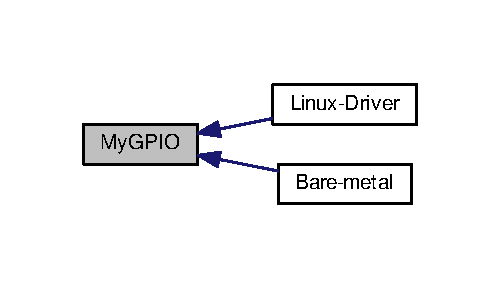
\includegraphics[width=240pt]{group__my_g_p_i_o}
\end{center}
\end{figure}
\subsection*{Moduli}
\begin{DoxyCompactItemize}
\item 
\hyperlink{group___linux-_driver}{Linux-\/\+Driver}
\end{DoxyCompactItemize}
\subsection*{Strutture dati}
\begin{DoxyCompactItemize}
\item 
struct \hyperlink{structmy_g_p_i_o__t}{my\+G\+P\+I\+O\+\_\+t}
\begin{DoxyCompactList}\small\item\em Struttura che astrae un device my\+G\+P\+I\+O. \end{DoxyCompactList}\end{DoxyCompactItemize}
\subsection*{Definizioni}
\begin{DoxyCompactItemize}
\item 
\#define \hyperlink{group__my_g_p_i_o_ga81a662103d6ed053978c0a9b4c273065}{my\+G\+P\+I\+O\+\_\+\+M\+O\+D\+E\+\_\+\+O\+F\+F\+S\+E\+T}~0\+U
\begin{DoxyCompactList}\small\item\em Offset, rispetto all'indirizzo base, del registro \char`\"{}mode\char`\"{} per il device my\+G\+P\+I\+O. \end{DoxyCompactList}\item 
\#define \hyperlink{group__my_g_p_i_o_ga2e45778b6ca9ce6f5768b3f7a4557ce1}{my\+G\+P\+I\+O\+\_\+\+W\+R\+I\+T\+E\+\_\+\+O\+F\+F\+S\+E\+T}~4\+U
\begin{DoxyCompactList}\small\item\em Offset, rispetto all'indirizzo base, del registro \char`\"{}write\char`\"{} per il device my\+G\+P\+I\+O. \end{DoxyCompactList}\item 
\#define \hyperlink{group__my_g_p_i_o_ga584d2dfece76e5762030d918d80592cc}{my\+G\+P\+I\+O\+\_\+\+R\+E\+A\+D\+\_\+\+O\+F\+F\+S\+E\+T}~8\+U
\begin{DoxyCompactList}\small\item\em Offset, rispetto all'indirizzo base, del registro \char`\"{}read\char`\"{} per il device my\+G\+P\+I\+O. \end{DoxyCompactList}\item 
\#define \hyperlink{group__my_g_p_i_o_gaacf2d8a21a051e778f02f8811b9c1e96}{my\+G\+P\+I\+O\+\_\+\+I\+N\+T\+R\+\_\+\+O\+F\+F\+S\+E\+T}~12\+U
\begin{DoxyCompactList}\small\item\em Offset, rispetto all'indirizzo base, del registro \char`\"{}interrupt\char`\"{} per il device my\+G\+P\+I\+O. \end{DoxyCompactList}\item 
\#define \hyperlink{group__my_g_p_i_o_ga0ba32e2adf874ed7216c5993369153e1}{my\+G\+P\+I\+O\+\_\+\+I\+N\+T\+R\+\_\+\+Int\+En\+\_\+mask}~0x1\+U
\begin{DoxyCompactList}\small\item\em maschera del bit del registro \char`\"{}interrupt\char`\"{} che funge da interrupt-\/enable, per il device my\+G\+P\+I\+O \end{DoxyCompactList}\item 
\#define \hyperlink{group__my_g_p_i_o_ga4cd02635783bc2a4ad7639cfb9fdb698}{my\+G\+P\+I\+O\+\_\+\+I\+N\+T\+R\+\_\+\+Irq\+\_\+mask}~0x2\+U
\begin{DoxyCompactList}\small\item\em maschera del bit del registro \char`\"{}interrupt\char`\"{} che funge da interrupt-\/request, per il device my\+G\+P\+I\+O \end{DoxyCompactList}\item 
\#define \hyperlink{group__my_g_p_i_o_gaa760b8397e6372e48c1008c2ba8d7387}{my\+G\+P\+I\+O\+\_\+\+I\+N\+T\+R\+\_\+\+Int\+Ack\+\_\+mask}~0x4\+U
\begin{DoxyCompactList}\small\item\em maschera del bit del registro \char`\"{}interrupt\char`\"{} che funge da interrupt-\/ack, per il device my\+G\+P\+I\+O \end{DoxyCompactList}\item 
\#define \hyperlink{group__my_g_p_i_o_gabbe2491a3b71c292521025b7b382b971}{my\+G\+P\+I\+O\+\_\+pin}(i)~((uint32\+\_\+t)(1$<$$<$(i)))
\begin{DoxyCompactList}\small\item\em Metodo alternativo per la specifica di uno dei pin di un device my\+G\+P\+I\+O. \end{DoxyCompactList}\end{DoxyCompactItemize}
\subsection*{Tipi enumerati (enum)}
\begin{DoxyCompactItemize}
\item 
enum \hyperlink{group__my_g_p_i_o_ga402a0d20afc0cb7c25554b8b023f4253}{my\+G\+P\+I\+O\+\_\+mask} \{ \\*
\hyperlink{group__my_g_p_i_o_gga402a0d20afc0cb7c25554b8b023f4253a6db6fa7be955ae379f543d96122e23a9}{my\+G\+P\+I\+O\+\_\+pin0} = 0x1\+U, 
\hyperlink{group__my_g_p_i_o_gga402a0d20afc0cb7c25554b8b023f4253a1de6bdcc01efca2c39f584f5a20293be}{my\+G\+P\+I\+O\+\_\+pin1} = 0x2\+U, 
\hyperlink{group__my_g_p_i_o_gga402a0d20afc0cb7c25554b8b023f4253a1fb3f52d920ac8ba17b74dd73c27d783}{my\+G\+P\+I\+O\+\_\+pin2} = 0x4\+U, 
\hyperlink{group__my_g_p_i_o_gga402a0d20afc0cb7c25554b8b023f4253a4514d64390392b626aa4dbfaac8dc1e5}{my\+G\+P\+I\+O\+\_\+pin3} = 0x8\+U, 
\\*
\hyperlink{group__my_g_p_i_o_gga402a0d20afc0cb7c25554b8b023f4253a0a446f53dee6f6f4ccb9a1d1f947b637}{my\+G\+P\+I\+O\+\_\+pin4} = 0x10\+U, 
\hyperlink{group__my_g_p_i_o_gga402a0d20afc0cb7c25554b8b023f4253a04a111036a27e9b97f0950f6d37b04d2}{my\+G\+P\+I\+O\+\_\+pin5} = 0x20\+U, 
\hyperlink{group__my_g_p_i_o_gga402a0d20afc0cb7c25554b8b023f4253a39a529f8c0a4f302029f54daa815471b}{my\+G\+P\+I\+O\+\_\+pin6} = 0x40\+U, 
\hyperlink{group__my_g_p_i_o_gga402a0d20afc0cb7c25554b8b023f4253af4e88b077442e4c0f459e1e4aa60626b}{my\+G\+P\+I\+O\+\_\+pin7} = 0x80\+U, 
\\*
\hyperlink{group__my_g_p_i_o_gga402a0d20afc0cb7c25554b8b023f4253a615159bcf4e347dc2b60f2545fae5f9e}{my\+G\+P\+I\+O\+\_\+pin8} = 0x100\+U, 
\hyperlink{group__my_g_p_i_o_gga402a0d20afc0cb7c25554b8b023f4253a8d721236fb936126a08c12b87696f6e9}{my\+G\+P\+I\+O\+\_\+pin9} = 0x200\+U, 
\hyperlink{group__my_g_p_i_o_gga402a0d20afc0cb7c25554b8b023f4253ae3067b7b3b1a2e171ecd74b6abd48341}{my\+G\+P\+I\+O\+\_\+pin10} = 0x400\+U, 
\hyperlink{group__my_g_p_i_o_gga402a0d20afc0cb7c25554b8b023f4253ae5c2e65508bfd452100d9da331d6220a}{my\+G\+P\+I\+O\+\_\+pin11} = 0x800\+U, 
\\*
\hyperlink{group__my_g_p_i_o_gga402a0d20afc0cb7c25554b8b023f4253afa75e3c1c019048c8553cb733c5137b5}{my\+G\+P\+I\+O\+\_\+pin12} = 0x1000\+U, 
\hyperlink{group__my_g_p_i_o_gga402a0d20afc0cb7c25554b8b023f4253a243381a796f0936a576f184dd115b37c}{my\+G\+P\+I\+O\+\_\+pin13} = 0x2000\+U, 
\hyperlink{group__my_g_p_i_o_gga402a0d20afc0cb7c25554b8b023f4253aed4915d6b3eab49cc1ba971b9f439fdd}{my\+G\+P\+I\+O\+\_\+pin14} = 0x4000\+U, 
\hyperlink{group__my_g_p_i_o_gga402a0d20afc0cb7c25554b8b023f4253a46c427ea97182a77e8c975d3429a64ee}{my\+G\+P\+I\+O\+\_\+pin15} = 0x8000\+U, 
\\*
\hyperlink{group__my_g_p_i_o_gga402a0d20afc0cb7c25554b8b023f4253a5a27c4d87207b2eba865876854f1ba67}{my\+G\+P\+I\+O\+\_\+pin16} = 0x10000\+U, 
\hyperlink{group__my_g_p_i_o_gga402a0d20afc0cb7c25554b8b023f4253ab0541af31059bdc8dca44d5dafa7e779}{my\+G\+P\+I\+O\+\_\+pin17} = 0x20000\+U, 
\hyperlink{group__my_g_p_i_o_gga402a0d20afc0cb7c25554b8b023f4253a7a51a492e3cb580581a2c8eb439edd99}{my\+G\+P\+I\+O\+\_\+pin18} = 0x40000\+U, 
\hyperlink{group__my_g_p_i_o_gga402a0d20afc0cb7c25554b8b023f4253a9118ae2775e93bd4522660e81a2d5309}{my\+G\+P\+I\+O\+\_\+pin19} = 0x80000\+U, 
\\*
\hyperlink{group__my_g_p_i_o_gga402a0d20afc0cb7c25554b8b023f4253a7940782a16f88dbbb3a4037c2bef1711}{my\+G\+P\+I\+O\+\_\+pin20} = 0x100000\+U, 
\hyperlink{group__my_g_p_i_o_gga402a0d20afc0cb7c25554b8b023f4253a1da616a8cf4396927db1e5a336fb6dc5}{my\+G\+P\+I\+O\+\_\+pin21} = 0x200000\+U, 
\hyperlink{group__my_g_p_i_o_gga402a0d20afc0cb7c25554b8b023f4253acf80113da8d789f7da9f9edc4ab6003c}{my\+G\+P\+I\+O\+\_\+pin22} = 0x400000\+U, 
\hyperlink{group__my_g_p_i_o_gga402a0d20afc0cb7c25554b8b023f4253ad64e03b703608de173ab5950b5121830}{my\+G\+P\+I\+O\+\_\+pin23} = 0x800000\+U, 
\\*
\hyperlink{group__my_g_p_i_o_gga402a0d20afc0cb7c25554b8b023f4253a5bb93f546327123f81b06ed0dfcdf110}{my\+G\+P\+I\+O\+\_\+pin24} = 0x1000000\+U, 
\hyperlink{group__my_g_p_i_o_gga402a0d20afc0cb7c25554b8b023f4253a0b27a7e78aff5836f33085f3b4539f56}{my\+G\+P\+I\+O\+\_\+pin25} = 0x2000000\+U, 
\hyperlink{group__my_g_p_i_o_gga402a0d20afc0cb7c25554b8b023f4253aaa07c24140250dcbc695206793efa8af}{my\+G\+P\+I\+O\+\_\+pin26} = 0x4000000\+U, 
\hyperlink{group__my_g_p_i_o_gga402a0d20afc0cb7c25554b8b023f4253a1dd5e99eba6237aeb30b2194c553c37f}{my\+G\+P\+I\+O\+\_\+pin27} = 0x8000000\+U, 
\\*
\hyperlink{group__my_g_p_i_o_gga402a0d20afc0cb7c25554b8b023f4253a2076590efec8bcf9ef3285798753e632}{my\+G\+P\+I\+O\+\_\+pin28} = 0x10000000\+U, 
\hyperlink{group__my_g_p_i_o_gga402a0d20afc0cb7c25554b8b023f4253abfe9540fa3946a35e20f7f68cb1b8084}{my\+G\+P\+I\+O\+\_\+pin29} = 0x20000000\+U, 
\hyperlink{group__my_g_p_i_o_gga402a0d20afc0cb7c25554b8b023f4253a59993a30c537c116eddb42d10778f4f8}{my\+G\+P\+I\+O\+\_\+pin30} = 0x40000000\+U, 
\hyperlink{group__my_g_p_i_o_gga402a0d20afc0cb7c25554b8b023f4253a9a55b7c245bd9aad750b7891d27e9225}{my\+G\+P\+I\+O\+\_\+pin31} = 0x80000000\+U, 
\\*
\hyperlink{group__my_g_p_i_o_gga402a0d20afc0cb7c25554b8b023f4253a0347b1742eef6b2575a7d409c7fb5c3d}{my\+G\+P\+I\+O\+\_\+byte0} = 0x000000ff\+U, 
\hyperlink{group__my_g_p_i_o_gga402a0d20afc0cb7c25554b8b023f4253ae5aec65fa20f554b893e419fc2755fd0}{my\+G\+P\+I\+O\+\_\+byte1} = 0x0000ff00\+U, 
\hyperlink{group__my_g_p_i_o_gga402a0d20afc0cb7c25554b8b023f4253af4892f7db28c64a7cf2a7236c88b742b}{my\+G\+P\+I\+O\+\_\+byte2} = 0x00ff0000\+U, 
\hyperlink{group__my_g_p_i_o_gga402a0d20afc0cb7c25554b8b023f4253a1ceefb9d65397352e986c573984d0129}{my\+G\+P\+I\+O\+\_\+byte3} = 0xff000000\+U
 \}
\begin{DoxyCompactList}\small\item\em Maschere di selezione dei pin di un device my\+G\+P\+I\+O. \end{DoxyCompactList}\item 
enum \hyperlink{group__my_g_p_i_o_ga76b849f0e0c05e7f9161bdb33396f2b1}{my\+G\+P\+I\+O\+\_\+mode} \{ \hyperlink{group__my_g_p_i_o_gga76b849f0e0c05e7f9161bdb33396f2b1a1e6dc78e7641e878cadc842d39605d5d}{my\+G\+P\+I\+O\+\_\+read}, 
\hyperlink{group__my_g_p_i_o_gga76b849f0e0c05e7f9161bdb33396f2b1a2d66976280eb7595a42c631683bdfad6}{my\+G\+P\+I\+O\+\_\+write}
 \}
\begin{DoxyCompactList}\small\item\em my\+G\+P\+I\+O\+\_\+mode, modalita' di funzionamento (lettura/scrittura) di un device my\+G\+P\+I\+O \end{DoxyCompactList}\item 
enum \hyperlink{group__my_g_p_i_o_gaf634fe4a0e1eab8da5000b72d6ad362b}{my\+G\+P\+I\+O\+\_\+value} \{ \hyperlink{group__my_g_p_i_o_ggaf634fe4a0e1eab8da5000b72d6ad362ba98cde80dbda025bd1ae7231c76b55674}{my\+G\+P\+I\+O\+\_\+reset}, 
\hyperlink{group__my_g_p_i_o_ggaf634fe4a0e1eab8da5000b72d6ad362ba10d296f3711d01189cc6c2d87f7c9149}{my\+G\+P\+I\+O\+\_\+set}
 \}
\begin{DoxyCompactList}\small\item\em my\+G\+P\+I\+O\+\_\+value, valore di un my\+G\+P\+I\+O \end{DoxyCompactList}\end{DoxyCompactItemize}
\subsection*{Funzioni}
\begin{DoxyCompactItemize}
\item 
void \hyperlink{group__my_g_p_i_o_ga8fda7ca73b187baf256409423c25d725}{my\+G\+P\+I\+O\+\_\+init} (\hyperlink{structmy_g_p_i_o__t}{my\+G\+P\+I\+O\+\_\+t} $\ast$gpio, uint32\+\_\+t base\+\_\+address)
\begin{DoxyCompactList}\small\item\em Inizializza un device my\+G\+P\+I\+O. \end{DoxyCompactList}\item 
void \hyperlink{group__my_g_p_i_o_ga38a2ea04d07af50f7f570f0367594c8b}{my\+G\+P\+I\+O\+\_\+set\+Mode} (\hyperlink{structmy_g_p_i_o__t}{my\+G\+P\+I\+O\+\_\+t} $\ast$gpio, \hyperlink{group__my_g_p_i_o_ga402a0d20afc0cb7c25554b8b023f4253}{my\+G\+P\+I\+O\+\_\+mask} mask, \hyperlink{group__my_g_p_i_o_ga76b849f0e0c05e7f9161bdb33396f2b1}{my\+G\+P\+I\+O\+\_\+mode} mode)
\begin{DoxyCompactList}\small\item\em Permette di settare la modalita' lettura/scrittura dei pin di un device my\+G\+P\+I\+O;. \end{DoxyCompactList}\item 
void \hyperlink{group__my_g_p_i_o_gab742e68093ad4c90fe299b64fd6736ca}{my\+G\+P\+I\+O\+\_\+set\+Value} (\hyperlink{structmy_g_p_i_o__t}{my\+G\+P\+I\+O\+\_\+t} $\ast$gpio, \hyperlink{group__my_g_p_i_o_ga402a0d20afc0cb7c25554b8b023f4253}{my\+G\+P\+I\+O\+\_\+mask} mask, \hyperlink{group__my_g_p_i_o_gaf634fe4a0e1eab8da5000b72d6ad362b}{my\+G\+P\+I\+O\+\_\+value} value)
\begin{DoxyCompactList}\small\item\em Permette di settare il valore dei pin di un device my\+G\+P\+I\+O, se configurati come output. \end{DoxyCompactList}\item 
void \hyperlink{group__my_g_p_i_o_ga27ea411bf51a58fe48eb8c5036780b53}{my\+G\+P\+I\+O\+\_\+toggle} (\hyperlink{structmy_g_p_i_o__t}{my\+G\+P\+I\+O\+\_\+t} $\ast$gpio, \hyperlink{group__my_g_p_i_o_ga402a0d20afc0cb7c25554b8b023f4253}{my\+G\+P\+I\+O\+\_\+mask} mask)
\begin{DoxyCompactList}\small\item\em Permette di invertire il valore dei pin di un device my\+G\+P\+I\+O, se configurati come output. \end{DoxyCompactList}\item 
\hyperlink{group__my_g_p_i_o_gaf634fe4a0e1eab8da5000b72d6ad362b}{my\+G\+P\+I\+O\+\_\+value} \hyperlink{group__my_g_p_i_o_gad6576f1d0fb17d9b492da0b1008550d0}{my\+G\+P\+I\+O\+\_\+get\+Value} (\hyperlink{structmy_g_p_i_o__t}{my\+G\+P\+I\+O\+\_\+t} $\ast$gpio, \hyperlink{group__my_g_p_i_o_ga402a0d20afc0cb7c25554b8b023f4253}{my\+G\+P\+I\+O\+\_\+mask} mask)
\begin{DoxyCompactList}\small\item\em Permette di leggere il valore dei pin di un device my\+G\+P\+I\+O;. \end{DoxyCompactList}\item 
\hyperlink{group__my_g_p_i_o_ga402a0d20afc0cb7c25554b8b023f4253}{my\+G\+P\+I\+O\+\_\+mask} \hyperlink{group__my_g_p_i_o_gadb3ecd03ea82420488977134c9313e18}{my\+G\+P\+I\+O\+\_\+get\+Read} (\hyperlink{structmy_g_p_i_o__t}{my\+G\+P\+I\+O\+\_\+t} $\ast$gpio)
\begin{DoxyCompactList}\small\item\em Restituisce la maschera dei pin settati di un device my\+G\+P\+I\+O. \end{DoxyCompactList}\item 
void \hyperlink{group__my_g_p_i_o_ga39822bfa495a9388e81ced74884c06a2}{my\+G\+P\+I\+O\+\_\+interrupt\+Enable} (\hyperlink{structmy_g_p_i_o__t}{my\+G\+P\+I\+O\+\_\+t} $\ast$gpio)
\begin{DoxyCompactList}\small\item\em Abilita gli interrupt per un device my\+G\+P\+I\+O. \end{DoxyCompactList}\item 
void \hyperlink{group__my_g_p_i_o_gab681db0119860bfad2c3e674289d8b3d}{my\+G\+P\+I\+O\+\_\+interrupt\+Disable} (\hyperlink{structmy_g_p_i_o__t}{my\+G\+P\+I\+O\+\_\+t} $\ast$gpio)
\begin{DoxyCompactList}\small\item\em Disabilita gli interrupt per un device my\+G\+P\+I\+O. \end{DoxyCompactList}\item 
void \hyperlink{group__my_g_p_i_o_ga396f6e5e7f0eeff01e98fcc78523402b}{my\+G\+P\+I\+O\+\_\+interrupt\+Ack} (\hyperlink{structmy_g_p_i_o__t}{my\+G\+P\+I\+O\+\_\+t} $\ast$gpio)
\begin{DoxyCompactList}\small\item\em Segnala al device che l'interruzione da lui sollevata e' stata servita. \end{DoxyCompactList}\item 
\hyperlink{group__my_g_p_i_o_gaf634fe4a0e1eab8da5000b72d6ad362b}{my\+G\+P\+I\+O\+\_\+value} \hyperlink{group__my_g_p_i_o_ga7936b506b45f116de68ddf06c84cc242}{my\+G\+P\+I\+O\+\_\+get\+Irq} (\hyperlink{structmy_g_p_i_o__t}{my\+G\+P\+I\+O\+\_\+t} $\ast$gpio)
\begin{DoxyCompactList}\small\item\em Consente di verificare se un device my\+G\+P\+I\+O abbia generato un'interruzione. \end{DoxyCompactList}\end{DoxyCompactItemize}


\subsection{Descrizione dettagliata}
Il modulo definisce un driver O\+O-\/like per l'utilizzo di una periferica my\+G\+P\+I\+O custom. 

\subsection{Documentazione delle definizioni}
\hypertarget{group__my_g_p_i_o_gaa760b8397e6372e48c1008c2ba8d7387}{\index{My\+G\+P\+I\+O@{My\+G\+P\+I\+O}!my\+G\+P\+I\+O\+\_\+\+I\+N\+T\+R\+\_\+\+Int\+Ack\+\_\+mask@{my\+G\+P\+I\+O\+\_\+\+I\+N\+T\+R\+\_\+\+Int\+Ack\+\_\+mask}}
\index{my\+G\+P\+I\+O\+\_\+\+I\+N\+T\+R\+\_\+\+Int\+Ack\+\_\+mask@{my\+G\+P\+I\+O\+\_\+\+I\+N\+T\+R\+\_\+\+Int\+Ack\+\_\+mask}!My\+G\+P\+I\+O@{My\+G\+P\+I\+O}}
\subsubsection[{my\+G\+P\+I\+O\+\_\+\+I\+N\+T\+R\+\_\+\+Int\+Ack\+\_\+mask}]{\setlength{\rightskip}{0pt plus 5cm}\#define my\+G\+P\+I\+O\+\_\+\+I\+N\+T\+R\+\_\+\+Int\+Ack\+\_\+mask~0x4\+U}}\label{group__my_g_p_i_o_gaa760b8397e6372e48c1008c2ba8d7387}


maschera del bit del registro \char`\"{}interrupt\char`\"{} che funge da interrupt-\/ack, per il device my\+G\+P\+I\+O 

\hypertarget{group__my_g_p_i_o_ga0ba32e2adf874ed7216c5993369153e1}{\index{My\+G\+P\+I\+O@{My\+G\+P\+I\+O}!my\+G\+P\+I\+O\+\_\+\+I\+N\+T\+R\+\_\+\+Int\+En\+\_\+mask@{my\+G\+P\+I\+O\+\_\+\+I\+N\+T\+R\+\_\+\+Int\+En\+\_\+mask}}
\index{my\+G\+P\+I\+O\+\_\+\+I\+N\+T\+R\+\_\+\+Int\+En\+\_\+mask@{my\+G\+P\+I\+O\+\_\+\+I\+N\+T\+R\+\_\+\+Int\+En\+\_\+mask}!My\+G\+P\+I\+O@{My\+G\+P\+I\+O}}
\subsubsection[{my\+G\+P\+I\+O\+\_\+\+I\+N\+T\+R\+\_\+\+Int\+En\+\_\+mask}]{\setlength{\rightskip}{0pt plus 5cm}\#define my\+G\+P\+I\+O\+\_\+\+I\+N\+T\+R\+\_\+\+Int\+En\+\_\+mask~0x1\+U}}\label{group__my_g_p_i_o_ga0ba32e2adf874ed7216c5993369153e1}


maschera del bit del registro \char`\"{}interrupt\char`\"{} che funge da interrupt-\/enable, per il device my\+G\+P\+I\+O 

\hypertarget{group__my_g_p_i_o_ga4cd02635783bc2a4ad7639cfb9fdb698}{\index{My\+G\+P\+I\+O@{My\+G\+P\+I\+O}!my\+G\+P\+I\+O\+\_\+\+I\+N\+T\+R\+\_\+\+Irq\+\_\+mask@{my\+G\+P\+I\+O\+\_\+\+I\+N\+T\+R\+\_\+\+Irq\+\_\+mask}}
\index{my\+G\+P\+I\+O\+\_\+\+I\+N\+T\+R\+\_\+\+Irq\+\_\+mask@{my\+G\+P\+I\+O\+\_\+\+I\+N\+T\+R\+\_\+\+Irq\+\_\+mask}!My\+G\+P\+I\+O@{My\+G\+P\+I\+O}}
\subsubsection[{my\+G\+P\+I\+O\+\_\+\+I\+N\+T\+R\+\_\+\+Irq\+\_\+mask}]{\setlength{\rightskip}{0pt plus 5cm}\#define my\+G\+P\+I\+O\+\_\+\+I\+N\+T\+R\+\_\+\+Irq\+\_\+mask~0x2\+U}}\label{group__my_g_p_i_o_ga4cd02635783bc2a4ad7639cfb9fdb698}


maschera del bit del registro \char`\"{}interrupt\char`\"{} che funge da interrupt-\/request, per il device my\+G\+P\+I\+O 

\hypertarget{group__my_g_p_i_o_gaacf2d8a21a051e778f02f8811b9c1e96}{\index{My\+G\+P\+I\+O@{My\+G\+P\+I\+O}!my\+G\+P\+I\+O\+\_\+\+I\+N\+T\+R\+\_\+\+O\+F\+F\+S\+E\+T@{my\+G\+P\+I\+O\+\_\+\+I\+N\+T\+R\+\_\+\+O\+F\+F\+S\+E\+T}}
\index{my\+G\+P\+I\+O\+\_\+\+I\+N\+T\+R\+\_\+\+O\+F\+F\+S\+E\+T@{my\+G\+P\+I\+O\+\_\+\+I\+N\+T\+R\+\_\+\+O\+F\+F\+S\+E\+T}!My\+G\+P\+I\+O@{My\+G\+P\+I\+O}}
\subsubsection[{my\+G\+P\+I\+O\+\_\+\+I\+N\+T\+R\+\_\+\+O\+F\+F\+S\+E\+T}]{\setlength{\rightskip}{0pt plus 5cm}\#define my\+G\+P\+I\+O\+\_\+\+I\+N\+T\+R\+\_\+\+O\+F\+F\+S\+E\+T~12\+U}}\label{group__my_g_p_i_o_gaacf2d8a21a051e778f02f8811b9c1e96}


Offset, rispetto all'indirizzo base, del registro \char`\"{}interrupt\char`\"{} per il device my\+G\+P\+I\+O. 

\hypertarget{group__my_g_p_i_o_ga81a662103d6ed053978c0a9b4c273065}{\index{My\+G\+P\+I\+O@{My\+G\+P\+I\+O}!my\+G\+P\+I\+O\+\_\+\+M\+O\+D\+E\+\_\+\+O\+F\+F\+S\+E\+T@{my\+G\+P\+I\+O\+\_\+\+M\+O\+D\+E\+\_\+\+O\+F\+F\+S\+E\+T}}
\index{my\+G\+P\+I\+O\+\_\+\+M\+O\+D\+E\+\_\+\+O\+F\+F\+S\+E\+T@{my\+G\+P\+I\+O\+\_\+\+M\+O\+D\+E\+\_\+\+O\+F\+F\+S\+E\+T}!My\+G\+P\+I\+O@{My\+G\+P\+I\+O}}
\subsubsection[{my\+G\+P\+I\+O\+\_\+\+M\+O\+D\+E\+\_\+\+O\+F\+F\+S\+E\+T}]{\setlength{\rightskip}{0pt plus 5cm}\#define my\+G\+P\+I\+O\+\_\+\+M\+O\+D\+E\+\_\+\+O\+F\+F\+S\+E\+T~0\+U}}\label{group__my_g_p_i_o_ga81a662103d6ed053978c0a9b4c273065}


Offset, rispetto all'indirizzo base, del registro \char`\"{}mode\char`\"{} per il device my\+G\+P\+I\+O. 

\hypertarget{group__my_g_p_i_o_gabbe2491a3b71c292521025b7b382b971}{\index{My\+G\+P\+I\+O@{My\+G\+P\+I\+O}!my\+G\+P\+I\+O\+\_\+pin@{my\+G\+P\+I\+O\+\_\+pin}}
\index{my\+G\+P\+I\+O\+\_\+pin@{my\+G\+P\+I\+O\+\_\+pin}!My\+G\+P\+I\+O@{My\+G\+P\+I\+O}}
\subsubsection[{my\+G\+P\+I\+O\+\_\+pin}]{\setlength{\rightskip}{0pt plus 5cm}\#define my\+G\+P\+I\+O\+\_\+pin(
\begin{DoxyParamCaption}
\item[{}]{i}
\end{DoxyParamCaption}
)~((uint32\+\_\+t)(1$<$$<$(i)))}}\label{group__my_g_p_i_o_gabbe2491a3b71c292521025b7b382b971}


Metodo alternativo per la specifica di uno dei pin di un device my\+G\+P\+I\+O. 


\begin{DoxyParams}[1]{Parametri}
\mbox{\tt in}  & {\em i} & indice del bit da selezionare, da 0 (bit meno significativo) a 31 (bit piu' significativo) \\
\hline
\end{DoxyParams}
\begin{DoxyReturn}{Restituisce}
maschera di selezione del pin i-\/esimo 
\end{DoxyReturn}
\hypertarget{group__my_g_p_i_o_ga584d2dfece76e5762030d918d80592cc}{\index{My\+G\+P\+I\+O@{My\+G\+P\+I\+O}!my\+G\+P\+I\+O\+\_\+\+R\+E\+A\+D\+\_\+\+O\+F\+F\+S\+E\+T@{my\+G\+P\+I\+O\+\_\+\+R\+E\+A\+D\+\_\+\+O\+F\+F\+S\+E\+T}}
\index{my\+G\+P\+I\+O\+\_\+\+R\+E\+A\+D\+\_\+\+O\+F\+F\+S\+E\+T@{my\+G\+P\+I\+O\+\_\+\+R\+E\+A\+D\+\_\+\+O\+F\+F\+S\+E\+T}!My\+G\+P\+I\+O@{My\+G\+P\+I\+O}}
\subsubsection[{my\+G\+P\+I\+O\+\_\+\+R\+E\+A\+D\+\_\+\+O\+F\+F\+S\+E\+T}]{\setlength{\rightskip}{0pt plus 5cm}\#define my\+G\+P\+I\+O\+\_\+\+R\+E\+A\+D\+\_\+\+O\+F\+F\+S\+E\+T~8\+U}}\label{group__my_g_p_i_o_ga584d2dfece76e5762030d918d80592cc}


Offset, rispetto all'indirizzo base, del registro \char`\"{}read\char`\"{} per il device my\+G\+P\+I\+O. 

\hypertarget{group__my_g_p_i_o_ga2e45778b6ca9ce6f5768b3f7a4557ce1}{\index{My\+G\+P\+I\+O@{My\+G\+P\+I\+O}!my\+G\+P\+I\+O\+\_\+\+W\+R\+I\+T\+E\+\_\+\+O\+F\+F\+S\+E\+T@{my\+G\+P\+I\+O\+\_\+\+W\+R\+I\+T\+E\+\_\+\+O\+F\+F\+S\+E\+T}}
\index{my\+G\+P\+I\+O\+\_\+\+W\+R\+I\+T\+E\+\_\+\+O\+F\+F\+S\+E\+T@{my\+G\+P\+I\+O\+\_\+\+W\+R\+I\+T\+E\+\_\+\+O\+F\+F\+S\+E\+T}!My\+G\+P\+I\+O@{My\+G\+P\+I\+O}}
\subsubsection[{my\+G\+P\+I\+O\+\_\+\+W\+R\+I\+T\+E\+\_\+\+O\+F\+F\+S\+E\+T}]{\setlength{\rightskip}{0pt plus 5cm}\#define my\+G\+P\+I\+O\+\_\+\+W\+R\+I\+T\+E\+\_\+\+O\+F\+F\+S\+E\+T~4\+U}}\label{group__my_g_p_i_o_ga2e45778b6ca9ce6f5768b3f7a4557ce1}


Offset, rispetto all'indirizzo base, del registro \char`\"{}write\char`\"{} per il device my\+G\+P\+I\+O. 



\subsection{Documentazione dei tipi enumerati}
\hypertarget{group__my_g_p_i_o_ga402a0d20afc0cb7c25554b8b023f4253}{\index{My\+G\+P\+I\+O@{My\+G\+P\+I\+O}!my\+G\+P\+I\+O\+\_\+mask@{my\+G\+P\+I\+O\+\_\+mask}}
\index{my\+G\+P\+I\+O\+\_\+mask@{my\+G\+P\+I\+O\+\_\+mask}!My\+G\+P\+I\+O@{My\+G\+P\+I\+O}}
\subsubsection[{my\+G\+P\+I\+O\+\_\+mask}]{\setlength{\rightskip}{0pt plus 5cm}enum {\bf my\+G\+P\+I\+O\+\_\+mask}}}\label{group__my_g_p_i_o_ga402a0d20afc0cb7c25554b8b023f4253}


Maschere di selezione dei pin di un device my\+G\+P\+I\+O. 

\begin{Desc}
\item[Valori del tipo enumerato]\par
\begin{description}
\index{my\+G\+P\+I\+O\+\_\+pin0@{my\+G\+P\+I\+O\+\_\+pin0}!My\+G\+P\+I\+O@{My\+G\+P\+I\+O}}\index{My\+G\+P\+I\+O@{My\+G\+P\+I\+O}!my\+G\+P\+I\+O\+\_\+pin0@{my\+G\+P\+I\+O\+\_\+pin0}}\item[{\em 
\hypertarget{group__my_g_p_i_o_gga402a0d20afc0cb7c25554b8b023f4253a6db6fa7be955ae379f543d96122e23a9}{my\+G\+P\+I\+O\+\_\+pin0}\label{group__my_g_p_i_o_gga402a0d20afc0cb7c25554b8b023f4253a6db6fa7be955ae379f543d96122e23a9}
}]my\+G\+P\+I\+O pin0 maschera di selezione del pin 0 di un device my\+G\+P\+I\+O \index{my\+G\+P\+I\+O\+\_\+pin1@{my\+G\+P\+I\+O\+\_\+pin1}!My\+G\+P\+I\+O@{My\+G\+P\+I\+O}}\index{My\+G\+P\+I\+O@{My\+G\+P\+I\+O}!my\+G\+P\+I\+O\+\_\+pin1@{my\+G\+P\+I\+O\+\_\+pin1}}\item[{\em 
\hypertarget{group__my_g_p_i_o_gga402a0d20afc0cb7c25554b8b023f4253a1de6bdcc01efca2c39f584f5a20293be}{my\+G\+P\+I\+O\+\_\+pin1}\label{group__my_g_p_i_o_gga402a0d20afc0cb7c25554b8b023f4253a1de6bdcc01efca2c39f584f5a20293be}
}]my\+G\+P\+I\+O pin1 maschera di selezione del pin 1 di un device my\+G\+P\+I\+O \index{my\+G\+P\+I\+O\+\_\+pin2@{my\+G\+P\+I\+O\+\_\+pin2}!My\+G\+P\+I\+O@{My\+G\+P\+I\+O}}\index{My\+G\+P\+I\+O@{My\+G\+P\+I\+O}!my\+G\+P\+I\+O\+\_\+pin2@{my\+G\+P\+I\+O\+\_\+pin2}}\item[{\em 
\hypertarget{group__my_g_p_i_o_gga402a0d20afc0cb7c25554b8b023f4253a1fb3f52d920ac8ba17b74dd73c27d783}{my\+G\+P\+I\+O\+\_\+pin2}\label{group__my_g_p_i_o_gga402a0d20afc0cb7c25554b8b023f4253a1fb3f52d920ac8ba17b74dd73c27d783}
}]my\+G\+P\+I\+O pin2 maschera di selezione del pin 2 di un device my\+G\+P\+I\+O \index{my\+G\+P\+I\+O\+\_\+pin3@{my\+G\+P\+I\+O\+\_\+pin3}!My\+G\+P\+I\+O@{My\+G\+P\+I\+O}}\index{My\+G\+P\+I\+O@{My\+G\+P\+I\+O}!my\+G\+P\+I\+O\+\_\+pin3@{my\+G\+P\+I\+O\+\_\+pin3}}\item[{\em 
\hypertarget{group__my_g_p_i_o_gga402a0d20afc0cb7c25554b8b023f4253a4514d64390392b626aa4dbfaac8dc1e5}{my\+G\+P\+I\+O\+\_\+pin3}\label{group__my_g_p_i_o_gga402a0d20afc0cb7c25554b8b023f4253a4514d64390392b626aa4dbfaac8dc1e5}
}]my\+G\+P\+I\+O pin3 maschera di selezione del pin 3 di un device my\+G\+P\+I\+O \index{my\+G\+P\+I\+O\+\_\+pin4@{my\+G\+P\+I\+O\+\_\+pin4}!My\+G\+P\+I\+O@{My\+G\+P\+I\+O}}\index{My\+G\+P\+I\+O@{My\+G\+P\+I\+O}!my\+G\+P\+I\+O\+\_\+pin4@{my\+G\+P\+I\+O\+\_\+pin4}}\item[{\em 
\hypertarget{group__my_g_p_i_o_gga402a0d20afc0cb7c25554b8b023f4253a0a446f53dee6f6f4ccb9a1d1f947b637}{my\+G\+P\+I\+O\+\_\+pin4}\label{group__my_g_p_i_o_gga402a0d20afc0cb7c25554b8b023f4253a0a446f53dee6f6f4ccb9a1d1f947b637}
}]my\+G\+P\+I\+O pin4 maschera di selezione del pin 4 di un device my\+G\+P\+I\+O \index{my\+G\+P\+I\+O\+\_\+pin5@{my\+G\+P\+I\+O\+\_\+pin5}!My\+G\+P\+I\+O@{My\+G\+P\+I\+O}}\index{My\+G\+P\+I\+O@{My\+G\+P\+I\+O}!my\+G\+P\+I\+O\+\_\+pin5@{my\+G\+P\+I\+O\+\_\+pin5}}\item[{\em 
\hypertarget{group__my_g_p_i_o_gga402a0d20afc0cb7c25554b8b023f4253a04a111036a27e9b97f0950f6d37b04d2}{my\+G\+P\+I\+O\+\_\+pin5}\label{group__my_g_p_i_o_gga402a0d20afc0cb7c25554b8b023f4253a04a111036a27e9b97f0950f6d37b04d2}
}]my\+G\+P\+I\+O pin5 maschera di selezione del pin 5 di un device my\+G\+P\+I\+O \index{my\+G\+P\+I\+O\+\_\+pin6@{my\+G\+P\+I\+O\+\_\+pin6}!My\+G\+P\+I\+O@{My\+G\+P\+I\+O}}\index{My\+G\+P\+I\+O@{My\+G\+P\+I\+O}!my\+G\+P\+I\+O\+\_\+pin6@{my\+G\+P\+I\+O\+\_\+pin6}}\item[{\em 
\hypertarget{group__my_g_p_i_o_gga402a0d20afc0cb7c25554b8b023f4253a39a529f8c0a4f302029f54daa815471b}{my\+G\+P\+I\+O\+\_\+pin6}\label{group__my_g_p_i_o_gga402a0d20afc0cb7c25554b8b023f4253a39a529f8c0a4f302029f54daa815471b}
}]my\+G\+P\+I\+O pin6 maschera di selezione del pin 6 di un device my\+G\+P\+I\+O \index{my\+G\+P\+I\+O\+\_\+pin7@{my\+G\+P\+I\+O\+\_\+pin7}!My\+G\+P\+I\+O@{My\+G\+P\+I\+O}}\index{My\+G\+P\+I\+O@{My\+G\+P\+I\+O}!my\+G\+P\+I\+O\+\_\+pin7@{my\+G\+P\+I\+O\+\_\+pin7}}\item[{\em 
\hypertarget{group__my_g_p_i_o_gga402a0d20afc0cb7c25554b8b023f4253af4e88b077442e4c0f459e1e4aa60626b}{my\+G\+P\+I\+O\+\_\+pin7}\label{group__my_g_p_i_o_gga402a0d20afc0cb7c25554b8b023f4253af4e88b077442e4c0f459e1e4aa60626b}
}]my\+G\+P\+I\+O pin7 maschera di selezione del pin 7 di un device my\+G\+P\+I\+O \index{my\+G\+P\+I\+O\+\_\+pin8@{my\+G\+P\+I\+O\+\_\+pin8}!My\+G\+P\+I\+O@{My\+G\+P\+I\+O}}\index{My\+G\+P\+I\+O@{My\+G\+P\+I\+O}!my\+G\+P\+I\+O\+\_\+pin8@{my\+G\+P\+I\+O\+\_\+pin8}}\item[{\em 
\hypertarget{group__my_g_p_i_o_gga402a0d20afc0cb7c25554b8b023f4253a615159bcf4e347dc2b60f2545fae5f9e}{my\+G\+P\+I\+O\+\_\+pin8}\label{group__my_g_p_i_o_gga402a0d20afc0cb7c25554b8b023f4253a615159bcf4e347dc2b60f2545fae5f9e}
}]my\+G\+P\+I\+O pin8 maschera di selezione del pin 8 di un device my\+G\+P\+I\+O \index{my\+G\+P\+I\+O\+\_\+pin9@{my\+G\+P\+I\+O\+\_\+pin9}!My\+G\+P\+I\+O@{My\+G\+P\+I\+O}}\index{My\+G\+P\+I\+O@{My\+G\+P\+I\+O}!my\+G\+P\+I\+O\+\_\+pin9@{my\+G\+P\+I\+O\+\_\+pin9}}\item[{\em 
\hypertarget{group__my_g_p_i_o_gga402a0d20afc0cb7c25554b8b023f4253a8d721236fb936126a08c12b87696f6e9}{my\+G\+P\+I\+O\+\_\+pin9}\label{group__my_g_p_i_o_gga402a0d20afc0cb7c25554b8b023f4253a8d721236fb936126a08c12b87696f6e9}
}]my\+G\+P\+I\+O pin9 maschera di selezione del pin 9 di un device my\+G\+P\+I\+O \index{my\+G\+P\+I\+O\+\_\+pin10@{my\+G\+P\+I\+O\+\_\+pin10}!My\+G\+P\+I\+O@{My\+G\+P\+I\+O}}\index{My\+G\+P\+I\+O@{My\+G\+P\+I\+O}!my\+G\+P\+I\+O\+\_\+pin10@{my\+G\+P\+I\+O\+\_\+pin10}}\item[{\em 
\hypertarget{group__my_g_p_i_o_gga402a0d20afc0cb7c25554b8b023f4253ae3067b7b3b1a2e171ecd74b6abd48341}{my\+G\+P\+I\+O\+\_\+pin10}\label{group__my_g_p_i_o_gga402a0d20afc0cb7c25554b8b023f4253ae3067b7b3b1a2e171ecd74b6abd48341}
}]my\+G\+P\+I\+O pin10 maschera di selezione del pin 10 di un device my\+G\+P\+I\+O \index{my\+G\+P\+I\+O\+\_\+pin11@{my\+G\+P\+I\+O\+\_\+pin11}!My\+G\+P\+I\+O@{My\+G\+P\+I\+O}}\index{My\+G\+P\+I\+O@{My\+G\+P\+I\+O}!my\+G\+P\+I\+O\+\_\+pin11@{my\+G\+P\+I\+O\+\_\+pin11}}\item[{\em 
\hypertarget{group__my_g_p_i_o_gga402a0d20afc0cb7c25554b8b023f4253ae5c2e65508bfd452100d9da331d6220a}{my\+G\+P\+I\+O\+\_\+pin11}\label{group__my_g_p_i_o_gga402a0d20afc0cb7c25554b8b023f4253ae5c2e65508bfd452100d9da331d6220a}
}]my\+G\+P\+I\+O pin11 maschera di selezione del pin 11 di un device my\+G\+P\+I\+O \index{my\+G\+P\+I\+O\+\_\+pin12@{my\+G\+P\+I\+O\+\_\+pin12}!My\+G\+P\+I\+O@{My\+G\+P\+I\+O}}\index{My\+G\+P\+I\+O@{My\+G\+P\+I\+O}!my\+G\+P\+I\+O\+\_\+pin12@{my\+G\+P\+I\+O\+\_\+pin12}}\item[{\em 
\hypertarget{group__my_g_p_i_o_gga402a0d20afc0cb7c25554b8b023f4253afa75e3c1c019048c8553cb733c5137b5}{my\+G\+P\+I\+O\+\_\+pin12}\label{group__my_g_p_i_o_gga402a0d20afc0cb7c25554b8b023f4253afa75e3c1c019048c8553cb733c5137b5}
}]my\+G\+P\+I\+O pin12 maschera di selezione del pin 12 di un device my\+G\+P\+I\+O \index{my\+G\+P\+I\+O\+\_\+pin13@{my\+G\+P\+I\+O\+\_\+pin13}!My\+G\+P\+I\+O@{My\+G\+P\+I\+O}}\index{My\+G\+P\+I\+O@{My\+G\+P\+I\+O}!my\+G\+P\+I\+O\+\_\+pin13@{my\+G\+P\+I\+O\+\_\+pin13}}\item[{\em 
\hypertarget{group__my_g_p_i_o_gga402a0d20afc0cb7c25554b8b023f4253a243381a796f0936a576f184dd115b37c}{my\+G\+P\+I\+O\+\_\+pin13}\label{group__my_g_p_i_o_gga402a0d20afc0cb7c25554b8b023f4253a243381a796f0936a576f184dd115b37c}
}]my\+G\+P\+I\+O pin13 maschera di selezione del pin 13 di un device my\+G\+P\+I\+O \index{my\+G\+P\+I\+O\+\_\+pin14@{my\+G\+P\+I\+O\+\_\+pin14}!My\+G\+P\+I\+O@{My\+G\+P\+I\+O}}\index{My\+G\+P\+I\+O@{My\+G\+P\+I\+O}!my\+G\+P\+I\+O\+\_\+pin14@{my\+G\+P\+I\+O\+\_\+pin14}}\item[{\em 
\hypertarget{group__my_g_p_i_o_gga402a0d20afc0cb7c25554b8b023f4253aed4915d6b3eab49cc1ba971b9f439fdd}{my\+G\+P\+I\+O\+\_\+pin14}\label{group__my_g_p_i_o_gga402a0d20afc0cb7c25554b8b023f4253aed4915d6b3eab49cc1ba971b9f439fdd}
}]my\+G\+P\+I\+O pin14 maschera di selezione del pin 14 di un device my\+G\+P\+I\+O \index{my\+G\+P\+I\+O\+\_\+pin15@{my\+G\+P\+I\+O\+\_\+pin15}!My\+G\+P\+I\+O@{My\+G\+P\+I\+O}}\index{My\+G\+P\+I\+O@{My\+G\+P\+I\+O}!my\+G\+P\+I\+O\+\_\+pin15@{my\+G\+P\+I\+O\+\_\+pin15}}\item[{\em 
\hypertarget{group__my_g_p_i_o_gga402a0d20afc0cb7c25554b8b023f4253a46c427ea97182a77e8c975d3429a64ee}{my\+G\+P\+I\+O\+\_\+pin15}\label{group__my_g_p_i_o_gga402a0d20afc0cb7c25554b8b023f4253a46c427ea97182a77e8c975d3429a64ee}
}]my\+G\+P\+I\+O pin15 maschera di selezione del pin 15 di un device my\+G\+P\+I\+O \index{my\+G\+P\+I\+O\+\_\+pin16@{my\+G\+P\+I\+O\+\_\+pin16}!My\+G\+P\+I\+O@{My\+G\+P\+I\+O}}\index{My\+G\+P\+I\+O@{My\+G\+P\+I\+O}!my\+G\+P\+I\+O\+\_\+pin16@{my\+G\+P\+I\+O\+\_\+pin16}}\item[{\em 
\hypertarget{group__my_g_p_i_o_gga402a0d20afc0cb7c25554b8b023f4253a5a27c4d87207b2eba865876854f1ba67}{my\+G\+P\+I\+O\+\_\+pin16}\label{group__my_g_p_i_o_gga402a0d20afc0cb7c25554b8b023f4253a5a27c4d87207b2eba865876854f1ba67}
}]my\+G\+P\+I\+O pin16 maschera di selezione del pin 16 di un device my\+G\+P\+I\+O \index{my\+G\+P\+I\+O\+\_\+pin17@{my\+G\+P\+I\+O\+\_\+pin17}!My\+G\+P\+I\+O@{My\+G\+P\+I\+O}}\index{My\+G\+P\+I\+O@{My\+G\+P\+I\+O}!my\+G\+P\+I\+O\+\_\+pin17@{my\+G\+P\+I\+O\+\_\+pin17}}\item[{\em 
\hypertarget{group__my_g_p_i_o_gga402a0d20afc0cb7c25554b8b023f4253ab0541af31059bdc8dca44d5dafa7e779}{my\+G\+P\+I\+O\+\_\+pin17}\label{group__my_g_p_i_o_gga402a0d20afc0cb7c25554b8b023f4253ab0541af31059bdc8dca44d5dafa7e779}
}]my\+G\+P\+I\+O pin17 maschera di selezione del pin 17 di un device my\+G\+P\+I\+O \index{my\+G\+P\+I\+O\+\_\+pin18@{my\+G\+P\+I\+O\+\_\+pin18}!My\+G\+P\+I\+O@{My\+G\+P\+I\+O}}\index{My\+G\+P\+I\+O@{My\+G\+P\+I\+O}!my\+G\+P\+I\+O\+\_\+pin18@{my\+G\+P\+I\+O\+\_\+pin18}}\item[{\em 
\hypertarget{group__my_g_p_i_o_gga402a0d20afc0cb7c25554b8b023f4253a7a51a492e3cb580581a2c8eb439edd99}{my\+G\+P\+I\+O\+\_\+pin18}\label{group__my_g_p_i_o_gga402a0d20afc0cb7c25554b8b023f4253a7a51a492e3cb580581a2c8eb439edd99}
}]my\+G\+P\+I\+O pin18 maschera di selezione del pin 18 di un device my\+G\+P\+I\+O \index{my\+G\+P\+I\+O\+\_\+pin19@{my\+G\+P\+I\+O\+\_\+pin19}!My\+G\+P\+I\+O@{My\+G\+P\+I\+O}}\index{My\+G\+P\+I\+O@{My\+G\+P\+I\+O}!my\+G\+P\+I\+O\+\_\+pin19@{my\+G\+P\+I\+O\+\_\+pin19}}\item[{\em 
\hypertarget{group__my_g_p_i_o_gga402a0d20afc0cb7c25554b8b023f4253a9118ae2775e93bd4522660e81a2d5309}{my\+G\+P\+I\+O\+\_\+pin19}\label{group__my_g_p_i_o_gga402a0d20afc0cb7c25554b8b023f4253a9118ae2775e93bd4522660e81a2d5309}
}]my\+G\+P\+I\+O pin19 maschera di selezione del pin 19 di un device my\+G\+P\+I\+O \index{my\+G\+P\+I\+O\+\_\+pin20@{my\+G\+P\+I\+O\+\_\+pin20}!My\+G\+P\+I\+O@{My\+G\+P\+I\+O}}\index{My\+G\+P\+I\+O@{My\+G\+P\+I\+O}!my\+G\+P\+I\+O\+\_\+pin20@{my\+G\+P\+I\+O\+\_\+pin20}}\item[{\em 
\hypertarget{group__my_g_p_i_o_gga402a0d20afc0cb7c25554b8b023f4253a7940782a16f88dbbb3a4037c2bef1711}{my\+G\+P\+I\+O\+\_\+pin20}\label{group__my_g_p_i_o_gga402a0d20afc0cb7c25554b8b023f4253a7940782a16f88dbbb3a4037c2bef1711}
}]my\+G\+P\+I\+O pin20 maschera di selezione del pin 20 di un device my\+G\+P\+I\+O \index{my\+G\+P\+I\+O\+\_\+pin21@{my\+G\+P\+I\+O\+\_\+pin21}!My\+G\+P\+I\+O@{My\+G\+P\+I\+O}}\index{My\+G\+P\+I\+O@{My\+G\+P\+I\+O}!my\+G\+P\+I\+O\+\_\+pin21@{my\+G\+P\+I\+O\+\_\+pin21}}\item[{\em 
\hypertarget{group__my_g_p_i_o_gga402a0d20afc0cb7c25554b8b023f4253a1da616a8cf4396927db1e5a336fb6dc5}{my\+G\+P\+I\+O\+\_\+pin21}\label{group__my_g_p_i_o_gga402a0d20afc0cb7c25554b8b023f4253a1da616a8cf4396927db1e5a336fb6dc5}
}]my\+G\+P\+I\+O pin21 maschera di selezione del pin 21 di un device my\+G\+P\+I\+O \index{my\+G\+P\+I\+O\+\_\+pin22@{my\+G\+P\+I\+O\+\_\+pin22}!My\+G\+P\+I\+O@{My\+G\+P\+I\+O}}\index{My\+G\+P\+I\+O@{My\+G\+P\+I\+O}!my\+G\+P\+I\+O\+\_\+pin22@{my\+G\+P\+I\+O\+\_\+pin22}}\item[{\em 
\hypertarget{group__my_g_p_i_o_gga402a0d20afc0cb7c25554b8b023f4253acf80113da8d789f7da9f9edc4ab6003c}{my\+G\+P\+I\+O\+\_\+pin22}\label{group__my_g_p_i_o_gga402a0d20afc0cb7c25554b8b023f4253acf80113da8d789f7da9f9edc4ab6003c}
}]my\+G\+P\+I\+O pin22 maschera di selezione del pin 22 di un device my\+G\+P\+I\+O \index{my\+G\+P\+I\+O\+\_\+pin23@{my\+G\+P\+I\+O\+\_\+pin23}!My\+G\+P\+I\+O@{My\+G\+P\+I\+O}}\index{My\+G\+P\+I\+O@{My\+G\+P\+I\+O}!my\+G\+P\+I\+O\+\_\+pin23@{my\+G\+P\+I\+O\+\_\+pin23}}\item[{\em 
\hypertarget{group__my_g_p_i_o_gga402a0d20afc0cb7c25554b8b023f4253ad64e03b703608de173ab5950b5121830}{my\+G\+P\+I\+O\+\_\+pin23}\label{group__my_g_p_i_o_gga402a0d20afc0cb7c25554b8b023f4253ad64e03b703608de173ab5950b5121830}
}]my\+G\+P\+I\+O pin23 maschera di selezione del pin 23 di un device my\+G\+P\+I\+O \index{my\+G\+P\+I\+O\+\_\+pin24@{my\+G\+P\+I\+O\+\_\+pin24}!My\+G\+P\+I\+O@{My\+G\+P\+I\+O}}\index{My\+G\+P\+I\+O@{My\+G\+P\+I\+O}!my\+G\+P\+I\+O\+\_\+pin24@{my\+G\+P\+I\+O\+\_\+pin24}}\item[{\em 
\hypertarget{group__my_g_p_i_o_gga402a0d20afc0cb7c25554b8b023f4253a5bb93f546327123f81b06ed0dfcdf110}{my\+G\+P\+I\+O\+\_\+pin24}\label{group__my_g_p_i_o_gga402a0d20afc0cb7c25554b8b023f4253a5bb93f546327123f81b06ed0dfcdf110}
}]my\+G\+P\+I\+O pin24 maschera di selezione del pin 24 di un device my\+G\+P\+I\+O \index{my\+G\+P\+I\+O\+\_\+pin25@{my\+G\+P\+I\+O\+\_\+pin25}!My\+G\+P\+I\+O@{My\+G\+P\+I\+O}}\index{My\+G\+P\+I\+O@{My\+G\+P\+I\+O}!my\+G\+P\+I\+O\+\_\+pin25@{my\+G\+P\+I\+O\+\_\+pin25}}\item[{\em 
\hypertarget{group__my_g_p_i_o_gga402a0d20afc0cb7c25554b8b023f4253a0b27a7e78aff5836f33085f3b4539f56}{my\+G\+P\+I\+O\+\_\+pin25}\label{group__my_g_p_i_o_gga402a0d20afc0cb7c25554b8b023f4253a0b27a7e78aff5836f33085f3b4539f56}
}]my\+G\+P\+I\+O pin25 maschera di selezione del pin 25 di un device my\+G\+P\+I\+O \index{my\+G\+P\+I\+O\+\_\+pin26@{my\+G\+P\+I\+O\+\_\+pin26}!My\+G\+P\+I\+O@{My\+G\+P\+I\+O}}\index{My\+G\+P\+I\+O@{My\+G\+P\+I\+O}!my\+G\+P\+I\+O\+\_\+pin26@{my\+G\+P\+I\+O\+\_\+pin26}}\item[{\em 
\hypertarget{group__my_g_p_i_o_gga402a0d20afc0cb7c25554b8b023f4253aaa07c24140250dcbc695206793efa8af}{my\+G\+P\+I\+O\+\_\+pin26}\label{group__my_g_p_i_o_gga402a0d20afc0cb7c25554b8b023f4253aaa07c24140250dcbc695206793efa8af}
}]my\+G\+P\+I\+O pin26 maschera di selezione del pin 26 di un device my\+G\+P\+I\+O \index{my\+G\+P\+I\+O\+\_\+pin27@{my\+G\+P\+I\+O\+\_\+pin27}!My\+G\+P\+I\+O@{My\+G\+P\+I\+O}}\index{My\+G\+P\+I\+O@{My\+G\+P\+I\+O}!my\+G\+P\+I\+O\+\_\+pin27@{my\+G\+P\+I\+O\+\_\+pin27}}\item[{\em 
\hypertarget{group__my_g_p_i_o_gga402a0d20afc0cb7c25554b8b023f4253a1dd5e99eba6237aeb30b2194c553c37f}{my\+G\+P\+I\+O\+\_\+pin27}\label{group__my_g_p_i_o_gga402a0d20afc0cb7c25554b8b023f4253a1dd5e99eba6237aeb30b2194c553c37f}
}]my\+G\+P\+I\+O pin27 maschera di selezione del pin 27 di un device my\+G\+P\+I\+O \index{my\+G\+P\+I\+O\+\_\+pin28@{my\+G\+P\+I\+O\+\_\+pin28}!My\+G\+P\+I\+O@{My\+G\+P\+I\+O}}\index{My\+G\+P\+I\+O@{My\+G\+P\+I\+O}!my\+G\+P\+I\+O\+\_\+pin28@{my\+G\+P\+I\+O\+\_\+pin28}}\item[{\em 
\hypertarget{group__my_g_p_i_o_gga402a0d20afc0cb7c25554b8b023f4253a2076590efec8bcf9ef3285798753e632}{my\+G\+P\+I\+O\+\_\+pin28}\label{group__my_g_p_i_o_gga402a0d20afc0cb7c25554b8b023f4253a2076590efec8bcf9ef3285798753e632}
}]my\+G\+P\+I\+O pin28 maschera di selezione del pin 28 di un device my\+G\+P\+I\+O \index{my\+G\+P\+I\+O\+\_\+pin29@{my\+G\+P\+I\+O\+\_\+pin29}!My\+G\+P\+I\+O@{My\+G\+P\+I\+O}}\index{My\+G\+P\+I\+O@{My\+G\+P\+I\+O}!my\+G\+P\+I\+O\+\_\+pin29@{my\+G\+P\+I\+O\+\_\+pin29}}\item[{\em 
\hypertarget{group__my_g_p_i_o_gga402a0d20afc0cb7c25554b8b023f4253abfe9540fa3946a35e20f7f68cb1b8084}{my\+G\+P\+I\+O\+\_\+pin29}\label{group__my_g_p_i_o_gga402a0d20afc0cb7c25554b8b023f4253abfe9540fa3946a35e20f7f68cb1b8084}
}]my\+G\+P\+I\+O pin29 maschera di selezione del pin 29 di un device my\+G\+P\+I\+O \index{my\+G\+P\+I\+O\+\_\+pin30@{my\+G\+P\+I\+O\+\_\+pin30}!My\+G\+P\+I\+O@{My\+G\+P\+I\+O}}\index{My\+G\+P\+I\+O@{My\+G\+P\+I\+O}!my\+G\+P\+I\+O\+\_\+pin30@{my\+G\+P\+I\+O\+\_\+pin30}}\item[{\em 
\hypertarget{group__my_g_p_i_o_gga402a0d20afc0cb7c25554b8b023f4253a59993a30c537c116eddb42d10778f4f8}{my\+G\+P\+I\+O\+\_\+pin30}\label{group__my_g_p_i_o_gga402a0d20afc0cb7c25554b8b023f4253a59993a30c537c116eddb42d10778f4f8}
}]my\+G\+P\+I\+O pin30 maschera di selezione del pin 30 di un device my\+G\+P\+I\+O \index{my\+G\+P\+I\+O\+\_\+pin31@{my\+G\+P\+I\+O\+\_\+pin31}!My\+G\+P\+I\+O@{My\+G\+P\+I\+O}}\index{My\+G\+P\+I\+O@{My\+G\+P\+I\+O}!my\+G\+P\+I\+O\+\_\+pin31@{my\+G\+P\+I\+O\+\_\+pin31}}\item[{\em 
\hypertarget{group__my_g_p_i_o_gga402a0d20afc0cb7c25554b8b023f4253a9a55b7c245bd9aad750b7891d27e9225}{my\+G\+P\+I\+O\+\_\+pin31}\label{group__my_g_p_i_o_gga402a0d20afc0cb7c25554b8b023f4253a9a55b7c245bd9aad750b7891d27e9225}
}]my\+G\+P\+I\+O pin31 maschera di selezione del pin 31 di un device my\+G\+P\+I\+O \index{my\+G\+P\+I\+O\+\_\+byte0@{my\+G\+P\+I\+O\+\_\+byte0}!My\+G\+P\+I\+O@{My\+G\+P\+I\+O}}\index{My\+G\+P\+I\+O@{My\+G\+P\+I\+O}!my\+G\+P\+I\+O\+\_\+byte0@{my\+G\+P\+I\+O\+\_\+byte0}}\item[{\em 
\hypertarget{group__my_g_p_i_o_gga402a0d20afc0cb7c25554b8b023f4253a0347b1742eef6b2575a7d409c7fb5c3d}{my\+G\+P\+I\+O\+\_\+byte0}\label{group__my_g_p_i_o_gga402a0d20afc0cb7c25554b8b023f4253a0347b1742eef6b2575a7d409c7fb5c3d}
}]my\+G\+P\+I\+O byte0 maschera di selezione de\+I pin 0-\/7 di un device my\+G\+P\+I\+O \index{my\+G\+P\+I\+O\+\_\+byte1@{my\+G\+P\+I\+O\+\_\+byte1}!My\+G\+P\+I\+O@{My\+G\+P\+I\+O}}\index{My\+G\+P\+I\+O@{My\+G\+P\+I\+O}!my\+G\+P\+I\+O\+\_\+byte1@{my\+G\+P\+I\+O\+\_\+byte1}}\item[{\em 
\hypertarget{group__my_g_p_i_o_gga402a0d20afc0cb7c25554b8b023f4253ae5aec65fa20f554b893e419fc2755fd0}{my\+G\+P\+I\+O\+\_\+byte1}\label{group__my_g_p_i_o_gga402a0d20afc0cb7c25554b8b023f4253ae5aec65fa20f554b893e419fc2755fd0}
}]my\+G\+P\+I\+O byte1 maschera di selezione de\+I pin 8-\/15 di un device my\+G\+P\+I\+O \index{my\+G\+P\+I\+O\+\_\+byte2@{my\+G\+P\+I\+O\+\_\+byte2}!My\+G\+P\+I\+O@{My\+G\+P\+I\+O}}\index{My\+G\+P\+I\+O@{My\+G\+P\+I\+O}!my\+G\+P\+I\+O\+\_\+byte2@{my\+G\+P\+I\+O\+\_\+byte2}}\item[{\em 
\hypertarget{group__my_g_p_i_o_gga402a0d20afc0cb7c25554b8b023f4253af4892f7db28c64a7cf2a7236c88b742b}{my\+G\+P\+I\+O\+\_\+byte2}\label{group__my_g_p_i_o_gga402a0d20afc0cb7c25554b8b023f4253af4892f7db28c64a7cf2a7236c88b742b}
}]my\+G\+P\+I\+O byte2 maschera di selezione de\+I pin 16-\/23 di un device my\+G\+P\+I\+O \index{my\+G\+P\+I\+O\+\_\+byte3@{my\+G\+P\+I\+O\+\_\+byte3}!My\+G\+P\+I\+O@{My\+G\+P\+I\+O}}\index{My\+G\+P\+I\+O@{My\+G\+P\+I\+O}!my\+G\+P\+I\+O\+\_\+byte3@{my\+G\+P\+I\+O\+\_\+byte3}}\item[{\em 
\hypertarget{group__my_g_p_i_o_gga402a0d20afc0cb7c25554b8b023f4253a1ceefb9d65397352e986c573984d0129}{my\+G\+P\+I\+O\+\_\+byte3}\label{group__my_g_p_i_o_gga402a0d20afc0cb7c25554b8b023f4253a1ceefb9d65397352e986c573984d0129}
}]my\+G\+P\+I\+O byte3 maschera di selezione de\+I pin 24-\/31 di un device my\+G\+P\+I\+O \end{description}
\end{Desc}
\hypertarget{group__my_g_p_i_o_ga76b849f0e0c05e7f9161bdb33396f2b1}{\index{My\+G\+P\+I\+O@{My\+G\+P\+I\+O}!my\+G\+P\+I\+O\+\_\+mode@{my\+G\+P\+I\+O\+\_\+mode}}
\index{my\+G\+P\+I\+O\+\_\+mode@{my\+G\+P\+I\+O\+\_\+mode}!My\+G\+P\+I\+O@{My\+G\+P\+I\+O}}
\subsubsection[{my\+G\+P\+I\+O\+\_\+mode}]{\setlength{\rightskip}{0pt plus 5cm}enum {\bf my\+G\+P\+I\+O\+\_\+mode}}}\label{group__my_g_p_i_o_ga76b849f0e0c05e7f9161bdb33396f2b1}


my\+G\+P\+I\+O\+\_\+mode, modalita' di funzionamento (lettura/scrittura) di un device my\+G\+P\+I\+O 

\begin{Desc}
\item[Valori del tipo enumerato]\par
\begin{description}
\index{my\+G\+P\+I\+O\+\_\+read@{my\+G\+P\+I\+O\+\_\+read}!My\+G\+P\+I\+O@{My\+G\+P\+I\+O}}\index{My\+G\+P\+I\+O@{My\+G\+P\+I\+O}!my\+G\+P\+I\+O\+\_\+read@{my\+G\+P\+I\+O\+\_\+read}}\item[{\em 
\hypertarget{group__my_g_p_i_o_gga76b849f0e0c05e7f9161bdb33396f2b1a1e6dc78e7641e878cadc842d39605d5d}{my\+G\+P\+I\+O\+\_\+read}\label{group__my_g_p_i_o_gga76b849f0e0c05e7f9161bdb33396f2b1a1e6dc78e7641e878cadc842d39605d5d}
}]my\+G\+P\+I\+O\+\_\+read modalita' lettura \index{my\+G\+P\+I\+O\+\_\+write@{my\+G\+P\+I\+O\+\_\+write}!My\+G\+P\+I\+O@{My\+G\+P\+I\+O}}\index{My\+G\+P\+I\+O@{My\+G\+P\+I\+O}!my\+G\+P\+I\+O\+\_\+write@{my\+G\+P\+I\+O\+\_\+write}}\item[{\em 
\hypertarget{group__my_g_p_i_o_gga76b849f0e0c05e7f9161bdb33396f2b1a2d66976280eb7595a42c631683bdfad6}{my\+G\+P\+I\+O\+\_\+write}\label{group__my_g_p_i_o_gga76b849f0e0c05e7f9161bdb33396f2b1a2d66976280eb7595a42c631683bdfad6}
}]my\+G\+P\+I\+O\+\_\+write modalita' scrittura \end{description}
\end{Desc}
\hypertarget{group__my_g_p_i_o_gaf634fe4a0e1eab8da5000b72d6ad362b}{\index{My\+G\+P\+I\+O@{My\+G\+P\+I\+O}!my\+G\+P\+I\+O\+\_\+value@{my\+G\+P\+I\+O\+\_\+value}}
\index{my\+G\+P\+I\+O\+\_\+value@{my\+G\+P\+I\+O\+\_\+value}!My\+G\+P\+I\+O@{My\+G\+P\+I\+O}}
\subsubsection[{my\+G\+P\+I\+O\+\_\+value}]{\setlength{\rightskip}{0pt plus 5cm}enum {\bf my\+G\+P\+I\+O\+\_\+value}}}\label{group__my_g_p_i_o_gaf634fe4a0e1eab8da5000b72d6ad362b}


my\+G\+P\+I\+O\+\_\+value, valore di un my\+G\+P\+I\+O 

\begin{Desc}
\item[Valori del tipo enumerato]\par
\begin{description}
\index{my\+G\+P\+I\+O\+\_\+reset@{my\+G\+P\+I\+O\+\_\+reset}!My\+G\+P\+I\+O@{My\+G\+P\+I\+O}}\index{My\+G\+P\+I\+O@{My\+G\+P\+I\+O}!my\+G\+P\+I\+O\+\_\+reset@{my\+G\+P\+I\+O\+\_\+reset}}\item[{\em 
\hypertarget{group__my_g_p_i_o_ggaf634fe4a0e1eab8da5000b72d6ad362ba98cde80dbda025bd1ae7231c76b55674}{my\+G\+P\+I\+O\+\_\+reset}\label{group__my_g_p_i_o_ggaf634fe4a0e1eab8da5000b72d6ad362ba98cde80dbda025bd1ae7231c76b55674}
}]my\+G\+P\+I\+O\+\_\+reset, corrisponde al valore logico '0' \index{my\+G\+P\+I\+O\+\_\+set@{my\+G\+P\+I\+O\+\_\+set}!My\+G\+P\+I\+O@{My\+G\+P\+I\+O}}\index{My\+G\+P\+I\+O@{My\+G\+P\+I\+O}!my\+G\+P\+I\+O\+\_\+set@{my\+G\+P\+I\+O\+\_\+set}}\item[{\em 
\hypertarget{group__my_g_p_i_o_ggaf634fe4a0e1eab8da5000b72d6ad362ba10d296f3711d01189cc6c2d87f7c9149}{my\+G\+P\+I\+O\+\_\+set}\label{group__my_g_p_i_o_ggaf634fe4a0e1eab8da5000b72d6ad362ba10d296f3711d01189cc6c2d87f7c9149}
}]my\+G\+P\+I\+O\+\_\+set, corrisponde al valore logico '1' \end{description}
\end{Desc}


\subsection{Documentazione delle funzioni}
\hypertarget{group__my_g_p_i_o_ga7936b506b45f116de68ddf06c84cc242}{\index{My\+G\+P\+I\+O@{My\+G\+P\+I\+O}!my\+G\+P\+I\+O\+\_\+get\+Irq@{my\+G\+P\+I\+O\+\_\+get\+Irq}}
\index{my\+G\+P\+I\+O\+\_\+get\+Irq@{my\+G\+P\+I\+O\+\_\+get\+Irq}!My\+G\+P\+I\+O@{My\+G\+P\+I\+O}}
\subsubsection[{my\+G\+P\+I\+O\+\_\+get\+Irq}]{\setlength{\rightskip}{0pt plus 5cm}{\bf my\+G\+P\+I\+O\+\_\+value} my\+G\+P\+I\+O\+\_\+get\+Irq (
\begin{DoxyParamCaption}
\item[{{\bf my\+G\+P\+I\+O\+\_\+t} $\ast$}]{gpio}
\end{DoxyParamCaption}
)}}\label{group__my_g_p_i_o_ga7936b506b45f116de68ddf06c84cc242}


Consente di verificare se un device my\+G\+P\+I\+O abbia generato un'interruzione. 


\begin{DoxyParams}[1]{Parametri}
\mbox{\tt in}  & {\em gpio} & puntatore a \hyperlink{structmy_g_p_i_o__t}{my\+G\+P\+I\+O\+\_\+t}, che astrae un device my\+G\+P\+I\+O;\\
\hline
\end{DoxyParams}

\begin{DoxyRetVals}{Valori di ritorno}
{\em my\+G\+P\+I\+O\+\_\+set} & se il device ha lanciato un'interruzione non ancora servita \\
\hline
{\em my\+G\+P\+I\+O\+\_\+reset} & se il device non ha interruzioni pendenti\\
\hline
\end{DoxyRetVals}

\begin{DoxyCode}
\end{DoxyCode}
 \hypertarget{group__my_g_p_i_o_gadb3ecd03ea82420488977134c9313e18}{\index{My\+G\+P\+I\+O@{My\+G\+P\+I\+O}!my\+G\+P\+I\+O\+\_\+get\+Read@{my\+G\+P\+I\+O\+\_\+get\+Read}}
\index{my\+G\+P\+I\+O\+\_\+get\+Read@{my\+G\+P\+I\+O\+\_\+get\+Read}!My\+G\+P\+I\+O@{My\+G\+P\+I\+O}}
\subsubsection[{my\+G\+P\+I\+O\+\_\+get\+Read}]{\setlength{\rightskip}{0pt plus 5cm}{\bf my\+G\+P\+I\+O\+\_\+mask} my\+G\+P\+I\+O\+\_\+get\+Read (
\begin{DoxyParamCaption}
\item[{{\bf my\+G\+P\+I\+O\+\_\+t} $\ast$}]{gpio}
\end{DoxyParamCaption}
)}}\label{group__my_g_p_i_o_gadb3ecd03ea82420488977134c9313e18}


Restituisce la maschera dei pin settati di un device my\+G\+P\+I\+O. 


\begin{DoxyParams}[1]{Parametri}
\mbox{\tt in}  & {\em gpio} & puntatore a \hyperlink{structmy_g_p_i_o__t}{my\+G\+P\+I\+O\+\_\+t}, che astrae un device my\+G\+P\+I\+O;\\
\hline
\end{DoxyParams}
\begin{DoxyReturn}{Restituisce}
maschera dei pin settati di un device my\+G\+P\+I\+O
\end{DoxyReturn}

\begin{DoxyCode}
1 myGPIO\_mask mask = myGPIO\_read(&gpio);
2 if (mask & myGPIO\_pin3) \{
3         ...
4 \}
5 else \{
6         ...
7 \}
\end{DoxyCode}
 \hypertarget{group__my_g_p_i_o_gad6576f1d0fb17d9b492da0b1008550d0}{\index{My\+G\+P\+I\+O@{My\+G\+P\+I\+O}!my\+G\+P\+I\+O\+\_\+get\+Value@{my\+G\+P\+I\+O\+\_\+get\+Value}}
\index{my\+G\+P\+I\+O\+\_\+get\+Value@{my\+G\+P\+I\+O\+\_\+get\+Value}!My\+G\+P\+I\+O@{My\+G\+P\+I\+O}}
\subsubsection[{my\+G\+P\+I\+O\+\_\+get\+Value}]{\setlength{\rightskip}{0pt plus 5cm}{\bf my\+G\+P\+I\+O\+\_\+value} my\+G\+P\+I\+O\+\_\+get\+Value (
\begin{DoxyParamCaption}
\item[{{\bf my\+G\+P\+I\+O\+\_\+t} $\ast$}]{gpio, }
\item[{{\bf my\+G\+P\+I\+O\+\_\+mask}}]{mask}
\end{DoxyParamCaption}
)}}\label{group__my_g_p_i_o_gad6576f1d0fb17d9b492da0b1008550d0}


Permette di leggere il valore dei pin di un device my\+G\+P\+I\+O;. 


\begin{DoxyCode}
1 // legge il valore del pin 0 di un device myGPIO.
2 myGPIO\_value value = gpio\_getValue(gpio, myGPIO\_pin0);
3 
4 // legge il valore del pin 0, 3 e 5 di un device myGPIO.
5 // Verra' restituita la OR tra i valori dei pin
6 myGPIO\_value value = gpio\_getValue(gpio, myGPIO\_pin0 | myGPIO\_pin3 | myGPIO\_pin5);
\end{DoxyCode}



\begin{DoxyParams}[1]{Parametri}
\mbox{\tt in}  & {\em gpio} & puntatore a \hyperlink{structmy_g_p_i_o__t}{my\+G\+P\+I\+O\+\_\+t}, che astrae un device my\+G\+P\+I\+O; \\
\hline
\mbox{\tt in}  & {\em mask} & maschera dei pin su cui agire;\\
\hline
\end{DoxyParams}
\begin{DoxyReturn}{Restituisce}
restituisce la O\+R dei pin letti 
\end{DoxyReturn}

\begin{DoxyRetVals}{Valori di ritorno}
{\em my\+G\+P\+I\+O\+\_\+set} & se uno dei pin letti e' my\+G\+P\+I\+O\+\_\+set, \\
\hline
{\em my\+G\+P\+I\+O\+\_\+reset} & se T\+U\+T\+T\+I i pin sono my\+G\+P\+I\+O\+\_\+reset\\
\hline
\end{DoxyRetVals}
\begin{DoxyWarning}{Avvertimento}
Usa la macro assert per verificare che gpio non sia un puntatore nullo 
\end{DoxyWarning}
\hypertarget{group__my_g_p_i_o_ga8fda7ca73b187baf256409423c25d725}{\index{My\+G\+P\+I\+O@{My\+G\+P\+I\+O}!my\+G\+P\+I\+O\+\_\+init@{my\+G\+P\+I\+O\+\_\+init}}
\index{my\+G\+P\+I\+O\+\_\+init@{my\+G\+P\+I\+O\+\_\+init}!My\+G\+P\+I\+O@{My\+G\+P\+I\+O}}
\subsubsection[{my\+G\+P\+I\+O\+\_\+init}]{\setlength{\rightskip}{0pt plus 5cm}void my\+G\+P\+I\+O\+\_\+init (
\begin{DoxyParamCaption}
\item[{{\bf my\+G\+P\+I\+O\+\_\+t} $\ast$}]{gpio, }
\item[{uint32\+\_\+t}]{base\+\_\+address}
\end{DoxyParamCaption}
)}}\label{group__my_g_p_i_o_ga8fda7ca73b187baf256409423c25d725}


Inizializza un device my\+G\+P\+I\+O. 

Inizializza una struttura di tipo \hyperlink{structmy_g_p_i_o__t}{my\+G\+P\+I\+O\+\_\+t}, che astrae u device my\+G\+P\+I\+O, controllando che l'inizializzazione vada a buon fine, effettuando diversi test sui parametri di inizializzazione e restituendo un codice di errore.


\begin{DoxyParams}[1]{Parametri}
\mbox{\tt in,out}  & {\em gpio} & puntatore a \hyperlink{structmy_g_p_i_o__t}{my\+G\+P\+I\+O\+\_\+t}, che astrae un device my\+G\+P\+I\+O; \\
\hline
\mbox{\tt in}  & {\em base\+\_\+address} & indirizzo di memoria a cui e' mappato il device my\+G\+P\+I\+O; 
\begin{DoxyCode}
1 myGPIO\_t gpio;
2 myGPIO\_init(&gpio, BASE\_ADDRESS);
\end{DoxyCode}
\\
\hline
\end{DoxyParams}
\begin{DoxyWarning}{Avvertimento}
Usa la macro assert per verificare che gpio e base\+\_\+address non siano nulli. 
\end{DoxyWarning}
\hypertarget{group__my_g_p_i_o_ga396f6e5e7f0eeff01e98fcc78523402b}{\index{My\+G\+P\+I\+O@{My\+G\+P\+I\+O}!my\+G\+P\+I\+O\+\_\+interrupt\+Ack@{my\+G\+P\+I\+O\+\_\+interrupt\+Ack}}
\index{my\+G\+P\+I\+O\+\_\+interrupt\+Ack@{my\+G\+P\+I\+O\+\_\+interrupt\+Ack}!My\+G\+P\+I\+O@{My\+G\+P\+I\+O}}
\subsubsection[{my\+G\+P\+I\+O\+\_\+interrupt\+Ack}]{\setlength{\rightskip}{0pt plus 5cm}void my\+G\+P\+I\+O\+\_\+interrupt\+Ack (
\begin{DoxyParamCaption}
\item[{{\bf my\+G\+P\+I\+O\+\_\+t} $\ast$}]{gpio}
\end{DoxyParamCaption}
)}}\label{group__my_g_p_i_o_ga396f6e5e7f0eeff01e98fcc78523402b}


Segnala al device che l'interruzione da lui sollevata e' stata servita. 


\begin{DoxyParams}[1]{Parametri}
\mbox{\tt in}  & {\em gpio} & puntatore a \hyperlink{structmy_g_p_i_o__t}{my\+G\+P\+I\+O\+\_\+t}, che astrae un device my\+G\+P\+I\+O;\\
\hline
\end{DoxyParams}

\begin{DoxyCode}
\end{DoxyCode}
 \hypertarget{group__my_g_p_i_o_gab681db0119860bfad2c3e674289d8b3d}{\index{My\+G\+P\+I\+O@{My\+G\+P\+I\+O}!my\+G\+P\+I\+O\+\_\+interrupt\+Disable@{my\+G\+P\+I\+O\+\_\+interrupt\+Disable}}
\index{my\+G\+P\+I\+O\+\_\+interrupt\+Disable@{my\+G\+P\+I\+O\+\_\+interrupt\+Disable}!My\+G\+P\+I\+O@{My\+G\+P\+I\+O}}
\subsubsection[{my\+G\+P\+I\+O\+\_\+interrupt\+Disable}]{\setlength{\rightskip}{0pt plus 5cm}void my\+G\+P\+I\+O\+\_\+interrupt\+Disable (
\begin{DoxyParamCaption}
\item[{{\bf my\+G\+P\+I\+O\+\_\+t} $\ast$}]{gpio}
\end{DoxyParamCaption}
)}}\label{group__my_g_p_i_o_gab681db0119860bfad2c3e674289d8b3d}


Disabilita gli interrupt per un device my\+G\+P\+I\+O. 


\begin{DoxyParams}[1]{Parametri}
\mbox{\tt in}  & {\em gpio} & puntatore a \hyperlink{structmy_g_p_i_o__t}{my\+G\+P\+I\+O\+\_\+t}, che astrae un device my\+G\+P\+I\+O;\\
\hline
\end{DoxyParams}

\begin{DoxyCode}
\end{DoxyCode}
 \hypertarget{group__my_g_p_i_o_ga39822bfa495a9388e81ced74884c06a2}{\index{My\+G\+P\+I\+O@{My\+G\+P\+I\+O}!my\+G\+P\+I\+O\+\_\+interrupt\+Enable@{my\+G\+P\+I\+O\+\_\+interrupt\+Enable}}
\index{my\+G\+P\+I\+O\+\_\+interrupt\+Enable@{my\+G\+P\+I\+O\+\_\+interrupt\+Enable}!My\+G\+P\+I\+O@{My\+G\+P\+I\+O}}
\subsubsection[{my\+G\+P\+I\+O\+\_\+interrupt\+Enable}]{\setlength{\rightskip}{0pt plus 5cm}void my\+G\+P\+I\+O\+\_\+interrupt\+Enable (
\begin{DoxyParamCaption}
\item[{{\bf my\+G\+P\+I\+O\+\_\+t} $\ast$}]{gpio}
\end{DoxyParamCaption}
)}}\label{group__my_g_p_i_o_ga39822bfa495a9388e81ced74884c06a2}


Abilita gli interrupt per un device my\+G\+P\+I\+O. 


\begin{DoxyParams}[1]{Parametri}
\mbox{\tt in}  & {\em gpio} & puntatore a \hyperlink{structmy_g_p_i_o__t}{my\+G\+P\+I\+O\+\_\+t}, che astrae un device my\+G\+P\+I\+O;\\
\hline
\end{DoxyParams}

\begin{DoxyCode}
1 //L'esempio seguente fa riferimento ad un sistema con un device myGPIO di 8 bit ai quali sono connessi
2 //led e button presenti sulla board Zybo.
3 //I led sono connessi ai bit 0-3 del device myGPIO, mentre i button sono connessi ai bit 4-7.
4 #include "xscugic.h"
5 #include "xparameters.h"
6 #include "myGPIO.h"
7 
8 #define myGPIO\_id           XPAR\_MYGPIO\_0\_DEVICE\_ID         // ID del device MYGPIO0
9 #define myGPIO\_addr         XPAR\_MYGPIO\_0\_S00\_AXI\_BASEADDR  // Indirizzo base del device MYGPIO0
10 #define myGPIO\_irq\_line     XPAR\_FABRIC\_MYGPIO\_0\_IRQ\_INTR   // linea interrupt a cui e' connesso il device
       MYGPIO0
11 #define GIC\_ID              XPAR\_SCUGIC\_0\_DEVICE\_ID         // ID del device GIC
12 #define GIC\_baddr           XPAR\_SCUGIC\_0\_CPU\_BASEADDR      // Indirizzo base del device GIC
13 
14 // funzione di configurazione delle interrupt
15 int INT\_config(XScuGic *GIC, myGPIO\_t* gpio);
16 
17 // prototipo della isr per la gestione della pressione di un button
18 // deve necessariamente essere una funzione che restituisce void e prende in ingresso un
19 // puntatore a void per i dati
20 void button\_isr(void* data);
21 
22 int main()
23 \{
24     XScuGic GIC;
25     myGPIO\_t gpio;
26 
27     myGPIO\_init(&gpio, myGPIO\_addr);
28     myGPIO\_setMode(&gpio, myGPIO\_pin0 | myGPIO\_pin1 | myGPIO\_pin2 | myGPIO\_pin3, myGPIO\_write);
29     myGPIO\_setMode(&gpio, myGPIO\_pin4 | myGPIO\_pin5 | myGPIO\_pin6 | myGPIO\_pin7, myGPIO\_read);
30     myGPIO\_setValue(&gpio, myGPIO\_pin0 | myGPIO\_pin1 | myGPIO\_pin2 | myGPIO\_pin3, myGPIO\_reset);
31 
32     INT\_config(&GIC, &gpio);
33 
34     for(;;);
35 
36     return 0;
37 \}
38 
39 int INT\_config(XScuGic *GIC, myGPIO\_t* gpio) \{
40 
41     // inizializza il driver del GIC
42     Xil\_ExceptionInit();
43 
44     // ottiene i parametri di configurazione del GIC, lo configura ed inizializza
45     // sintassi : XScuGic\_LookupConfig(GIC\_id)
46     // sintassi : XScuGic\_CfgInitialize(GIC, config, address)
47     XScuGic\_Config *IntcConfig = XScuGic\_LookupConfig(GIC\_ID);
48     if (IntcConfig == NULL)
49         return -1;
50     if (XScuGic\_CfgInitialize(GIC, IntcConfig, IntcConfig->CpuBaseAddress) != XST\_SUCCESS)
51         return -1;
52 
53     // registra l'interrupt handler del GIC alla logica di gestione del processing-system
54     Xil\_ExceptionRegisterHandler(XIL\_EXCEPTION\_ID\_INT,(Xil\_ExceptionHandler)XScuGic\_InterruptHandler, GIC);
55 
56     // registrazione degli handler
57     // le due righe seguenti stabiliscono quale sia l'handler da chiamare e quali dati bisogna passargli
58     // qualora si manifesti una interruzione su una line di irq.
59     // sintassi : XScuGic\_Connect(GIC, irq\_line, handler, data)
60     if (XScuGic\_Connect(GIC, myGPIO\_irq\_line, (Xil\_InterruptHandler)button\_isr, (void*)gpio) !=
       XST\_SUCCESS)
61         return -1;
62 
63     // abilitazione degli interrupt sulle linee connesse alle periferiche
64     // sintassi: XScuGic\_Enable(GIC,irq\_line);
65     XScuGic\_Enable(GIC, myGPIO\_irq\_line);
66     // abilitazione degli interrupt delle periferiche
67     myGPIO\_interruptEnable(gpio);
68 
69     // abilitazione degli interrupt del processing-system
70     Xil\_ExceptionEnable();
71 
72     return 0;
73 \}
74 
75 void button\_isr(void* data) \{
76     myGPIO\_t* gpio = (myGPIO\_t*)data;
77 
78     myGPIO\_interruptDisable(gpio);  // disabilito gli interrupt
79     myGPIO\_interruptAck(gpio);      // clear del flag irq
80 
81     myGPIO\_mask mask = myGPIO\_getRead(gpio);
82     myGPIO\_setValue(gpio, myGPIO\_pin0 | myGPIO\_pin1 | myGPIO\_pin2 | myGPIO\_pin3, myGPIO\_reset);
83     myGPIO\_setValue(gpio, mask>>4, myGPIO\_set);
84 
85     myGPIO\_value value = myGPIO\_getIrq(gpio);
86     myGPIO\_interruptAck(gpio);
87     value = myGPIO\_getIrq(gpio);
88     myGPIO\_setValue(gpio, myGPIO\_pin0 | myGPIO\_pin1 | myGPIO\_pin2 | myGPIO\_pin3, value);
89     myGPIO\_setValue(gpio, myGPIO\_pin0 | myGPIO\_pin1 | myGPIO\_pin2 | myGPIO\_pin3, value);
90 
91     myGPIO\_interruptEnable(gpio);   // ri-abilito gli interrupt
92 \}
\end{DoxyCode}
 
\begin{DoxyCode}
1 #include "xscugic.h"
2 #include "xparameters.h"
3 #include "myGPIO.h"
4 
5 #define btn\_addr    XPAR\_MYGPIO\_0\_S00\_AXI\_BASEADDR  // base-address del gpio connesso ai button
6 #define btn\_line    XPAR\_FABRIC\_MYGPIO\_0\_IRQ\_INTR   // linea di interrupt del gpio connesso ai button
7 #define swc\_addr    XPAR\_MYGPIO\_1\_S00\_AXI\_BASEADDR  // base-address del gpio connesso agli switch
8 #define swc\_line    XPAR\_FABRIC\_MYGPIO\_1\_IRQ\_INTR   // linea di interrupt del gpio connesso agli switch
9 #define led\_addr    XPAR\_MYGPIO\_2\_S00\_AXI\_BASEADDR  // base-address del gpio connesso ai led
10 
11 #define gic\_id      XPAR\_SCUGIC\_0\_DEVICE\_ID         // id del device gic
12 
13 myGPIO\_t led\_gpio;
14 myGPIO\_t btn\_gpio;
15 myGPIO\_t swc\_gpio;
16 XScuGic GIC;
17 
18 // funzione di inizializzazione dei device gpio
19 void gpio\_init(void);
20 
21 
22 // isr per button e switch
23 // devono necessariamente avere questa firma: restituire void e possedere un solo parametro puntatore
24 // a void. In questo caso non viene utilizzato (tutte le variabili sono globali), ma tale puntatore
25 // puo' essere usato per scambiare dati di ingresso/uscita alle isr
26 void btn\_isr(void*); // isr per i button
27 void swc\_isr(void*); // isr per gli switch
28 
29 // funzione di configurazione del device gic e delle interruzioni
30 int int\_config(void);
31 
32 int main()
33 \{
34     gpio\_init();
35     int\_config();
36 
37     for (;;);
38 
39     return 0;
40 \}
41 
42 
43 void gpio\_init(void) \{
44     uint8\_t i;
45     myGPIO\_init(&led\_gpio, led\_addr);
46     myGPIO\_init(&btn\_gpio, btn\_addr);
47     myGPIO\_init(&swc\_gpio, swc\_addr);
48     for (i=0; i<myGPIO\_pin4; i++) \{
49         myGPIO\_setMode(&led\_gpio, myGPIO\_pin(i), myGPIO\_write);
50         myGPIO\_setValue(&led\_gpio, myGPIO\_pin(i), myGPIO\_reset);
51         myGPIO\_setMode(&btn\_gpio, myGPIO\_pin(i), myGPIO\_read);
52         myGPIO\_setValue(&btn\_gpio, myGPIO\_pin(i), myGPIO\_reset);
53         myGPIO\_setMode(&swc\_gpio, myGPIO\_pin(i), myGPIO\_read);
54         myGPIO\_setValue(&swc\_gpio, myGPIO\_pin(i), myGPIO\_reset);
55     \}
56 \}
57 
58 int int\_config(void) \{
59     // inizializza il driver del GIC
60     Xil\_ExceptionInit();
61 
62     // ottiene i parametri di configurazione del GIC, lo configura ed inizializza
63     // sintassi : XScuGic\_LookupConfig(GIC\_id)
64     // sintassi : XScuGic\_CfgInitialize(GIC\_ptr, config, cpu\_address)
65     XScuGic\_Config *IntcConfig = XScuGic\_LookupConfig(gic\_id);
66     if (IntcConfig == NULL)
67         return -1;
68     if (XScuGic\_CfgInitialize(&GIC, IntcConfig, IntcConfig->CpuBaseAddress) != XST\_SUCCESS)
69         return -1;
70 
71     // registra l'interrupt handler del GIC alla logica di gestione del processing-system
72     // sintassi : Xil\_ExceptionRegisterHandler(XIL\_EXCEPTION\_ID\_INT, handler, gic\_ptr)
73     Xil\_ExceptionRegisterHandler(XIL\_EXCEPTION\_ID\_INT,(Xil\_ExceptionHandler)XScuGic\_InterruptHandler,
       &GIC);
74 
75     // registrazione degli handler
76     // le righe seguenti stabiliscono quale sia l'handler da chiamare e quali dati bisogna passargli
77     // qualora si manifesti una interruzione su una line di irq.
78     // sintassi : XScuGic\_Connect(GIC, irq\_line, handler, data)
79     if (XScuGic\_Connect(&GIC, btn\_line, (Xil\_InterruptHandler)btn\_isr, (void*)NULL) != XST\_SUCCESS)
80         return -1;
81     if (XScuGic\_Connect(&GIC, swc\_line, (Xil\_InterruptHandler)swc\_isr, (void*)NULL) != XST\_SUCCESS)
82             return -1;
83 
84     // abilitazione degli interrupt sulle linee connesse alle periferiche
85     // sintassi: XScuGic\_Enable(GIC,irq\_line);
86     XScuGic\_Enable(&GIC, btn\_line);
87     XScuGic\_Enable(&GIC, swc\_line);
88 
89     // abilitazione degli interrupt delle periferiche
90     myGPIO\_interruptEnable(&btn\_gpio);
91     myGPIO\_interruptEnable(&swc\_gpio);
92 
93     // abilitazione degli interrupt del processing-system
94     Xil\_ExceptionEnable();
95     return 0;
96 \}
97 
98 void btn\_isr(void* data) \{
99     myGPIO\_interruptDisable(&btn\_gpio); // disabilito gli interrupt
100     myGPIO\_interruptAck(&btn\_gpio);     // clear del flag irq
101     myGPIO\_mask mask = myGPIO\_getRead(&btn\_gpio);
102     myGPIO\_setValue(&led\_gpio, myGPIO\_pin0 | myGPIO\_pin1 | myGPIO\_pin2 | myGPIO\_pin3, myGPIO\_reset);
103     myGPIO\_setValue(&led\_gpio, mask, myGPIO\_set);
104     myGPIO\_interruptEnable(&btn\_gpio);  // ri-abilito gli interrupt
105 \}
106 
107 void swc\_isr(void* data) \{
108     myGPIO\_interruptDisable(&swc\_gpio); // disabilito gli interrupt
109     myGPIO\_interruptAck(&swc\_gpio);     // clear del flag irq
110     myGPIO\_mask mask = myGPIO\_getRead(&swc\_gpio);
111     myGPIO\_setValue(&led\_gpio, myGPIO\_pin0 | myGPIO\_pin1 | myGPIO\_pin2 | myGPIO\_pin3, myGPIO\_reset);
112     myGPIO\_setValue(&led\_gpio, mask, myGPIO\_set);
113     myGPIO\_interruptEnable(&swc\_gpio);  // ri-abilito gli interrupt
114 \}
\end{DoxyCode}
 \hypertarget{group__my_g_p_i_o_ga38a2ea04d07af50f7f570f0367594c8b}{\index{My\+G\+P\+I\+O@{My\+G\+P\+I\+O}!my\+G\+P\+I\+O\+\_\+set\+Mode@{my\+G\+P\+I\+O\+\_\+set\+Mode}}
\index{my\+G\+P\+I\+O\+\_\+set\+Mode@{my\+G\+P\+I\+O\+\_\+set\+Mode}!My\+G\+P\+I\+O@{My\+G\+P\+I\+O}}
\subsubsection[{my\+G\+P\+I\+O\+\_\+set\+Mode}]{\setlength{\rightskip}{0pt plus 5cm}void my\+G\+P\+I\+O\+\_\+set\+Mode (
\begin{DoxyParamCaption}
\item[{{\bf my\+G\+P\+I\+O\+\_\+t} $\ast$}]{gpio, }
\item[{{\bf my\+G\+P\+I\+O\+\_\+mask}}]{mask, }
\item[{{\bf my\+G\+P\+I\+O\+\_\+mode}}]{mode}
\end{DoxyParamCaption}
)}}\label{group__my_g_p_i_o_ga38a2ea04d07af50f7f570f0367594c8b}


Permette di settare la modalita' lettura/scrittura dei pin di un device my\+G\+P\+I\+O;. 


\begin{DoxyCode}
1 // setta i pin 0 ed 1 di un device myGPIO come pin di uscita, gli altri restano invariati
2 myGPIO\_setMode(gpio, myGPIO\_pin0 | myGPIO\_pin1, myGPIO\_write);
3 
4 // setta i pin 19, 20 e 21 di un device myGPIO come pin di ingresso, gli altri restano invariati
5 myGPIO\_setMode(gpio, myGPIO\_pin19 | myGPIO\_pin20 | myGPIO\_pin21, myGPIO\_read);
\end{DoxyCode}



\begin{DoxyParams}[1]{Parametri}
\mbox{\tt in}  & {\em gpio} & puntatore a \hyperlink{structmy_g_p_i_o__t}{my\+G\+P\+I\+O\+\_\+t}, che astrae un device my\+G\+P\+I\+O; \\
\hline
\mbox{\tt in}  & {\em mask} & maschera dei pin su cui agire; \\
\hline
\mbox{\tt in}  & {\em mode} & modalita' di funzionamento dei pin;\\
\hline
\end{DoxyParams}
\begin{DoxyWarning}{Avvertimento}
Usa la macro assert per verificare che gpio non sia un puntatore nullo 
\end{DoxyWarning}
\hypertarget{group__my_g_p_i_o_gab742e68093ad4c90fe299b64fd6736ca}{\index{My\+G\+P\+I\+O@{My\+G\+P\+I\+O}!my\+G\+P\+I\+O\+\_\+set\+Value@{my\+G\+P\+I\+O\+\_\+set\+Value}}
\index{my\+G\+P\+I\+O\+\_\+set\+Value@{my\+G\+P\+I\+O\+\_\+set\+Value}!My\+G\+P\+I\+O@{My\+G\+P\+I\+O}}
\subsubsection[{my\+G\+P\+I\+O\+\_\+set\+Value}]{\setlength{\rightskip}{0pt plus 5cm}void my\+G\+P\+I\+O\+\_\+set\+Value (
\begin{DoxyParamCaption}
\item[{{\bf my\+G\+P\+I\+O\+\_\+t} $\ast$}]{gpio, }
\item[{{\bf my\+G\+P\+I\+O\+\_\+mask}}]{mask, }
\item[{{\bf my\+G\+P\+I\+O\+\_\+value}}]{value}
\end{DoxyParamCaption}
)}}\label{group__my_g_p_i_o_gab742e68093ad4c90fe299b64fd6736ca}


Permette di settare il valore dei pin di un device my\+G\+P\+I\+O, se configurati come output. 


\begin{DoxyCode}
1 // setta i pin 0 ed 1 di un device myGPIO a livello logico '1', gli altri restano invariati
2 myGPIO\_setValue(gpio, myGPIO\_pin0 | myGPIO\_pin1, myGPIO\_set);
3 
4 // setta i pin 19, 20 e 21 di un device myGPIO a livello logico '0', gli altri restano invariati
5 myGPIO\_setValue(gpio, myGPIO\_pin19 | myGPIO\_pin20 | myGPIO\_pin21, myGPIO\_reset);
\end{DoxyCode}



\begin{DoxyParams}[1]{Parametri}
\mbox{\tt in}  & {\em gpio} & puntatore a \hyperlink{structmy_g_p_i_o__t}{my\+G\+P\+I\+O\+\_\+t}, che astrae un device my\+G\+P\+I\+O; \\
\hline
\mbox{\tt in}  & {\em mask} & maschera dei pin su cui agire; \\
\hline
\mbox{\tt in}  & {\em value} & valore dei pin\\
\hline
\end{DoxyParams}
\begin{DoxyWarning}{Avvertimento}
Usa la macro assert per verificare che gpio non sia un puntatore nullo 
\end{DoxyWarning}
\hypertarget{group__my_g_p_i_o_ga27ea411bf51a58fe48eb8c5036780b53}{\index{My\+G\+P\+I\+O@{My\+G\+P\+I\+O}!my\+G\+P\+I\+O\+\_\+toggle@{my\+G\+P\+I\+O\+\_\+toggle}}
\index{my\+G\+P\+I\+O\+\_\+toggle@{my\+G\+P\+I\+O\+\_\+toggle}!My\+G\+P\+I\+O@{My\+G\+P\+I\+O}}
\subsubsection[{my\+G\+P\+I\+O\+\_\+toggle}]{\setlength{\rightskip}{0pt plus 5cm}void my\+G\+P\+I\+O\+\_\+toggle (
\begin{DoxyParamCaption}
\item[{{\bf my\+G\+P\+I\+O\+\_\+t} $\ast$}]{gpio, }
\item[{{\bf my\+G\+P\+I\+O\+\_\+mask}}]{mask}
\end{DoxyParamCaption}
)}}\label{group__my_g_p_i_o_ga27ea411bf51a58fe48eb8c5036780b53}


Permette di invertire il valore dei pin di un device my\+G\+P\+I\+O, se configurati come output. 


\begin{DoxyCode}
1 // inverte i pin 0 ed 1 di un device myGPIO a livello logico '1', gli altri restano invariati
2 myGPIO\_toggle(gpio, myGPIO\_pin0 | myGPIO\_pin1);
\end{DoxyCode}



\begin{DoxyParams}[1]{Parametri}
\mbox{\tt in}  & {\em gpio} & puntatore a \hyperlink{structmy_g_p_i_o__t}{my\+G\+P\+I\+O\+\_\+t}, che astrae un device my\+G\+P\+I\+O; \\
\hline
\mbox{\tt in}  & {\em mask} & maschera dei pin su cui agire;\\
\hline
\end{DoxyParams}
\begin{DoxyWarning}{Avvertimento}
Usa la macro assert per verificare che gpio non sia un puntatore nullo 
\end{DoxyWarning}

\hypertarget{group___linux-_driver}{\section{Linux-\/\+Driver}
\label{group___linux-_driver}\index{Linux-\/\+Driver@{Linux-\/\+Driver}}
}


Device-\/driver in kernel-\/mode per my\+G\+P\+I\+O.  


Diagramma di collaborazione per Linux-\/\+Driver\+:\nopagebreak
\begin{figure}[H]
\begin{center}
\leavevmode
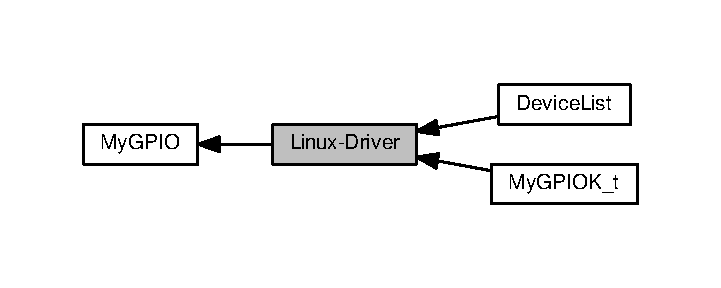
\includegraphics[width=240pt]{group___linux-_driver}
\end{center}
\end{figure}
\subsection*{Strutture dati}
\begin{DoxyCompactItemize}
\item 
struct \hyperlink{structmy_g_p_i_o_k__t}{my\+G\+P\+I\+O\+K\+\_\+t}
\begin{DoxyCompactList}\small\item\em Stuttura per l'astrazione di un device my\+G\+P\+I\+O in kernel-\/mode. \end{DoxyCompactList}\end{DoxyCompactItemize}
\subsection*{Definizioni}
\begin{DoxyCompactItemize}
\item 
\#define \hyperlink{group___linux-_driver_ga543e17293942b7cf7936a5e095ddc7ef}{my\+G\+P\+I\+O\+K\+\_\+\+M\+O\+D\+E\+\_\+\+O\+F\+F\+S\+E\+T}~0x00\+U
\begin{DoxyCompactList}\small\item\em Offset, rispetto all'indirizzo base, del registro \char`\"{}mode\char`\"{} per il device my\+G\+P\+I\+O. \end{DoxyCompactList}\item 
\#define \hyperlink{group___linux-_driver_gac165a5d828f3df41e78bb02d4ef38327}{my\+G\+P\+I\+O\+K\+\_\+\+W\+R\+I\+T\+E\+\_\+\+O\+F\+F\+S\+E\+T}~0x04\+U
\begin{DoxyCompactList}\small\item\em Offset, rispetto all'indirizzo base, del registro \char`\"{}write\char`\"{} per il device my\+G\+P\+I\+O. \end{DoxyCompactList}\item 
\#define \hyperlink{group___linux-_driver_gabdb25f3ecdfbf053f4ca207930a56599}{my\+G\+P\+I\+O\+K\+\_\+\+R\+E\+A\+D\+\_\+\+O\+F\+F\+S\+E\+T}~0x08\+U
\begin{DoxyCompactList}\small\item\em Offset, rispetto all'indirizzo base, del registro \char`\"{}read\char`\"{} per il device my\+G\+P\+I\+O. \end{DoxyCompactList}\item 
\#define \hyperlink{group___linux-_driver_ga0da2526ca3cd1a94ebcecf96778ea2e5}{my\+G\+P\+I\+O\+K\+\_\+\+G\+I\+E\+S\+\_\+\+O\+F\+F\+S\+E\+T}~0x0\+C\+U
\begin{DoxyCompactList}\small\item\em Offset, rispetto all'indirizzo base, del registro \char`\"{}gies\char`\"{} per il device my\+G\+P\+I\+O. \end{DoxyCompactList}\item 
\#define \hyperlink{group___linux-_driver_ga2ed7646e6f910f5803477e51b7fe26e3}{my\+G\+P\+I\+O\+K\+\_\+\+P\+I\+E\+\_\+\+O\+F\+F\+S\+E\+T}~0x10\+U
\begin{DoxyCompactList}\small\item\em Offset, rispetto all'indirizzo base, del registro \char`\"{}pie\char`\"{} per il device my\+G\+P\+I\+O. \end{DoxyCompactList}\item 
\#define \hyperlink{group___linux-_driver_ga37ee502d1ba364dfde9261c4f7a537a6}{my\+G\+P\+I\+O\+K\+\_\+\+I\+R\+Q\+\_\+\+O\+F\+F\+S\+E\+T}~0x14\+U
\begin{DoxyCompactList}\small\item\em Offset, rispetto all'indirizzo base, del registro \char`\"{}irq\char`\"{} per il device my\+G\+P\+I\+O. \end{DoxyCompactList}\item 
\#define \hyperlink{group___linux-_driver_gac72408c288009c213c0231973b3fe761}{my\+G\+P\+I\+O\+K\+\_\+\+I\+A\+C\+K\+\_\+\+O\+F\+F\+S\+E\+T}~0x18\+U
\begin{DoxyCompactList}\small\item\em Offset, rispetto all'indirizzo base, del registro \char`\"{}iack\char`\"{} per il device my\+G\+P\+I\+O. \end{DoxyCompactList}\item 
\#define \hyperlink{group___linux-_driver_ga78d3a23bb3381a43eaba8bbf8b1cc750}{my\+G\+P\+I\+O\+K\+\_\+\+U\+S\+E\+D\+\_\+\+I\+N\+T}~0x\+F\+F\+F\+F\+F\+F\+F\+F\+U
\begin{DoxyCompactList}\small\item\em Maschea di abilitazione degli interrupt per i singoli pin. \end{DoxyCompactList}\item 
\#define \hyperlink{group___linux-_driver_ga25634d21648ca7fb7a2aca614bafaaeb}{D\+R\+I\+V\+E\+R\+\_\+\+N\+A\+M\+E}~\char`\"{}my\+G\+P\+I\+O\+K\char`\"{}
\begin{DoxyCompactList}\small\item\em Nome identificativo del device-\/driver. D\+E\+V\+E corrispondere al valore del campo \char`\"{}compatible\char`\"{} nel device tree source. \end{DoxyCompactList}\item 
\#define \hyperlink{group___linux-_driver_gad32bf20eb64878cb958ca6ac9c96c21d}{M\+A\+X\+\_\+\+N\+U\+M\+\_\+\+O\+F\+\_\+\+D\+E\+V\+I\+C\+E\+S}~1
\begin{DoxyCompactList}\small\item\em Numero di minor-\/number richiesti dal driver, corrispondera' al numero massimo di device gestibili. \end{DoxyCompactList}\end{DoxyCompactItemize}
\subsection*{Funzioni}
\begin{DoxyCompactItemize}
\item 
static int \hyperlink{group___linux-_driver_gae40973a06d72f7c41a9af07513a62307}{my\+G\+P\+I\+O\+K\+\_\+probe} (struct platform\+\_\+device $\ast$op)
\begin{DoxyCompactList}\small\item\em Viene chiamata quando il modulo viene inserito. \end{DoxyCompactList}\item 
static int \hyperlink{group___linux-_driver_ga59fddfaa36dea357f4bbdfceb0f47f8c}{my\+G\+P\+I\+O\+K\+\_\+remove} (struct platform\+\_\+device $\ast$op)
\item 
static int \hyperlink{group___linux-_driver_gad013759c18fbf6ea96005b9b3bfa5b4e}{my\+G\+P\+I\+O\+K\+\_\+open} (struct inode $\ast$inode, struct file $\ast$file\+\_\+ptr)
\begin{DoxyCompactList}\small\item\em Invocata all'apertura del file corrispondente al device. \end{DoxyCompactList}\item 
static int \hyperlink{group___linux-_driver_ga17ce7f574723246c790b70b06e3e7103}{my\+G\+P\+I\+O\+K\+\_\+release} (struct inode $\ast$inode, struct file $\ast$file\+\_\+ptr)
\begin{DoxyCompactList}\small\item\em Invocata alla chiusura del file corrispondente al device. \end{DoxyCompactList}\item 
static loff\+\_\+t \hyperlink{group___linux-_driver_ga66e7f726b72320a272b633ecbaecefff}{my\+G\+P\+I\+O\+K\+\_\+llseek} (struct file $\ast$file\+\_\+ptr, loff\+\_\+t off, int whence)
\begin{DoxyCompactList}\small\item\em Implementa le system-\/call lseek() e llseek(). \end{DoxyCompactList}\item 
static unsigned int \hyperlink{group___linux-_driver_gaba935e8a8215c2ebce9a7147fd4f5147}{my\+G\+P\+I\+O\+K\+\_\+poll} (struct file $\ast$file\+\_\+ptr, struct poll\+\_\+table\+\_\+struct $\ast$wait)
\begin{DoxyCompactList}\small\item\em Verifica che le operazioni di lettura/scrittura risultino non-\/bloccanti. \end{DoxyCompactList}\item 
static ssize\+\_\+t \hyperlink{group___linux-_driver_ga90ac339df9c02ae5f11a2a7727adc923}{my\+G\+P\+I\+O\+K\+\_\+read} (struct file $\ast$file\+\_\+ptr, char $\ast$buf, size\+\_\+t count, loff\+\_\+t $\ast$off)
\begin{DoxyCompactList}\small\item\em Legge dati dal device. \end{DoxyCompactList}\item 
static ssize\+\_\+t \hyperlink{group___linux-_driver_ga1eea0f6c86e8966ba9b701da57502aad}{my\+G\+P\+I\+O\+K\+\_\+write} (struct file $\ast$file\+\_\+ptr, const char $\ast$buf, size\+\_\+t size, loff\+\_\+t $\ast$off)
\begin{DoxyCompactList}\small\item\em Invia dati al device. \end{DoxyCompactList}\item 
static irqreturn\+\_\+t \hyperlink{group___linux-_driver_ga2fc230a12a97aa63e43b2dc4aec73511}{my\+G\+P\+I\+O\+K\+\_\+irq\+\_\+handler} (int irq, struct pt\+\_\+regs $\ast$regs)
\begin{DoxyCompactList}\small\item\em Interrupt-\/handler. \end{DoxyCompactList}\item 
static void \hyperlink{group___linux-_driver_gabd22e9dc7675ba815f1dd8840b39b2bf}{my\+G\+P\+I\+O\+K\+\_\+\+Global\+Interrupt\+Enable} (void $\ast$base\+Address)
\begin{DoxyCompactList}\small\item\em Abilita gli interrupt globali;. \end{DoxyCompactList}\item 
static void \hyperlink{group___linux-_driver_ga941f5d329dffbf6e45cecd70bbc72b63}{my\+G\+P\+I\+O\+K\+\_\+\+Global\+Interrupt\+Disable} (void $\ast$base\+Address)
\begin{DoxyCompactList}\small\item\em Disabilita gli interrupt globali;. \end{DoxyCompactList}\item 
static void \hyperlink{group___linux-_driver_ga15ddb23be51d3e2dbb00278af7e9ce31}{my\+G\+P\+I\+O\+K\+\_\+\+Pin\+Interrupt\+Enable} (void $\ast$base\+Address, unsigned mask)
\begin{DoxyCompactList}\small\item\em Abilita gli interrupt per i singoli pin del device. \end{DoxyCompactList}\item 
static void \hyperlink{group___linux-_driver_ga57efe4a8be5e162cfd2e98f61d195087}{my\+G\+P\+I\+O\+K\+\_\+\+Pin\+Interrupt\+Disable} (void $\ast$base\+Address, unsigned mask)
\begin{DoxyCompactList}\small\item\em Disabilita gli interrupt per i singoli pin del device. \end{DoxyCompactList}\item 
static unsigned \hyperlink{group___linux-_driver_ga6019e1ca45d7a093e1e7fc546b16f773}{my\+G\+P\+I\+O\+K\+\_\+\+Pending\+Pin\+Interrupt} (void $\ast$base\+Address)
\begin{DoxyCompactList}\small\item\em Consente di ottenere una maschera che indichi quali interrupt non siano stati ancora serviti;. \end{DoxyCompactList}\item 
static void \hyperlink{group___linux-_driver_ga105156c3db48f9dd40300218e7d8e144}{my\+G\+P\+I\+O\+K\+\_\+\+Pin\+Interrupt\+Ack} (void $\ast$base\+Address, unsigned mask)
\begin{DoxyCompactList}\small\item\em Invia al device notifica di servizio di un interrupt;. \end{DoxyCompactList}\end{DoxyCompactItemize}
\subsection*{Variabili}
\begin{DoxyCompactItemize}
\item 
\hyperlink{structmy_g_p_i_o_k__t}{my\+G\+P\+I\+O\+K\+\_\+t} $\ast$ \hyperlink{group___linux-_driver_gae370dfc26b06b6cc24a7bcc152f4969e}{my\+G\+P\+I\+O\+K\+\_\+dev\+\_\+ptr} = N\+U\+L\+L
\begin{DoxyCompactList}\small\item\em Puntatore a struttura \hyperlink{structmy_g_p_i_o_k__t}{my\+G\+P\+I\+O\+K\+\_\+t}, contenente tutti i dati necessari al device driver. \end{DoxyCompactList}\item 
static dev\+\_\+t \hyperlink{group___linux-_driver_ga434e034e4625b1949f0c626823870a39}{my\+G\+P\+I\+O\+K\+\_\+\+Mm\+\_\+number}
\begin{DoxyCompactList}\small\item\em Major e minor number per il device driver. \end{DoxyCompactList}\item 
static struct class $\ast$ \hyperlink{group___linux-_driver_gaaf8d1bce7d6389684a037e94381c275c}{my\+G\+P\+I\+O\+K\+\_\+class} = N\+U\+L\+L
\item 
static struct device $\ast$ \hyperlink{group___linux-_driver_ga2d345c792760e3103059b6b6e0bfdaee}{my\+G\+P\+I\+O\+K\+\_\+device} = N\+U\+L\+L
\item 
static struct of\+\_\+device\+\_\+id \hyperlink{group___linux-_driver_ga91f28437e0a553effa546d16fa44f03a}{my\+G\+P\+I\+Ok\+\_\+match} \mbox{[}$\,$\mbox{]}
\begin{DoxyCompactList}\small\item\em Identifica il device all'interno del device tree. \end{DoxyCompactList}\item 
static struct platform\+\_\+driver \hyperlink{group___linux-_driver_ga8dba1541b58fa63f8208232ffce4fc47}{my\+G\+P\+I\+O\+K\+\_\+driver}
\begin{DoxyCompactList}\small\item\em Definisce quali funzioni probe() e remove() chiamare quando viene caricato un driver. \end{DoxyCompactList}\item 
static struct file\+\_\+operations \hyperlink{group___linux-_driver_ga9f31111fdb3b4a5944e18d45045e0f01}{my\+G\+P\+I\+O\+\_\+fops}
\begin{DoxyCompactList}\small\item\em mantiene puntatori a funzioni che definiscono il gli operatori che agiscono su un file/device. \end{DoxyCompactList}\end{DoxyCompactItemize}


\subsection{Descrizione dettagliata}
Device-\/driver in kernel-\/mode per my\+G\+P\+I\+O. 

\begin{DoxyWarning}{Avvertimento}
Se nel device tree source non viene indicato \begin{center}compatible = \char`\"{}my\+G\+P\+I\+O\+K\char`\"{};\end{center}  tra i driver compatibili con il device, il driver my\+G\+P\+I\+O\+K non viene correttamente istanziato ed il programma userspace non funzionera'.
\end{DoxyWarning}
\subsubsection*{Descrizione generale del driver}

Il modulo driver implementa definisce il tipo \hyperlink{structmy_g_p_i_o_k__t}{my\+G\+P\+I\+O\+K\+\_\+t} ed implementa le seguenti funzioni\+:
\begin{DoxyItemize}
\item \hyperlink{group___linux-_driver_gae40973a06d72f7c41a9af07513a62307}{my\+G\+P\+I\+O\+K\+\_\+probe()}\+: richiamata quando il modulo, o un device compatibile col modulo, viene inserito\+:
\item \hyperlink{group___linux-_driver_ga59fddfaa36dea357f4bbdfceb0f47f8c}{my\+G\+P\+I\+O\+K\+\_\+remove()}\+: richiamata quando il modulo, o un device compatibile, viene rimosso;
\item \hyperlink{group___linux-_driver_gad013759c18fbf6ea96005b9b3bfa5b4e}{my\+G\+P\+I\+O\+K\+\_\+open()}\+: implementa la system call open();
\item \hyperlink{group___linux-_driver_ga66e7f726b72320a272b633ecbaecefff}{my\+G\+P\+I\+O\+K\+\_\+llseek()}\+: implementa la system call seek();
\item \hyperlink{group___linux-_driver_ga1eea0f6c86e8966ba9b701da57502aad}{my\+G\+P\+I\+O\+K\+\_\+write()}\+: implementa la system call seek();
\item \hyperlink{group___linux-_driver_ga2fc230a12a97aa63e43b2dc4aec73511}{my\+G\+P\+I\+O\+K\+\_\+irq\+\_\+handler()}\+: implementa la I\+S\+R dedicata alla gestione delle interruzioni provenienti dal device;
\item \hyperlink{group___linux-_driver_gaba935e8a8215c2ebce9a7147fd4f5147}{my\+G\+P\+I\+O\+K\+\_\+poll()} \+: implementa il back-\/end di tre diverse system-\/calls (poll, epoll e select)
\item \hyperlink{group___linux-_driver_ga90ac339df9c02ae5f11a2a7727adc923}{my\+G\+P\+I\+O\+K\+\_\+read()} \+: implementa la system call read.
\end{DoxyItemize}

Nel seguito viene presentato un breve escursus su tutto cio' che c'e' da sapere per comprendere come funziona un device-\/driver e come poterne scrivere uno. Dopo aver letto il seguito, si consiglia, in ordine, di leggere, in ordine, la documentazione della struttura my\+G\+P\+I\+O\+K-\/t, poi quella delle funzioni
\begin{DoxyItemize}
\item \hyperlink{group___linux-_driver_gae40973a06d72f7c41a9af07513a62307}{my\+G\+P\+I\+O\+K\+\_\+probe()};
\item \hyperlink{group___linux-_driver_gad013759c18fbf6ea96005b9b3bfa5b4e}{my\+G\+P\+I\+O\+K\+\_\+open()};
\item \hyperlink{group___linux-_driver_ga66e7f726b72320a272b633ecbaecefff}{my\+G\+P\+I\+O\+K\+\_\+llseek()};
\item \hyperlink{group___linux-_driver_ga1eea0f6c86e8966ba9b701da57502aad}{my\+G\+P\+I\+O\+K\+\_\+write()};
\item \hyperlink{group___linux-_driver_ga90ac339df9c02ae5f11a2a7727adc923}{my\+G\+P\+I\+O\+K\+\_\+read()};
\item \hyperlink{group___linux-_driver_ga2fc230a12a97aa63e43b2dc4aec73511}{my\+G\+P\+I\+O\+K\+\_\+irq\+\_\+handler()};
\end{DoxyItemize}

\paragraph*{Platform-\/device}

I device driver, anche se sono moduli kernel, non si scrivono come normali moduli Kernel. I \char`\"{}platform-\/device\char`\"{} sono device che non possono annunciarsi al software (non possono dire \char`\"{}\+Hey,
sono qui'!\char`\"{} al sistema operativo), quindi sono intrinsecamente \char`\"{}non-\/scopribili\char`\"{}, nel senso che il sistema, al boot, deve sapere che ci sono, ma non e' in grado di scoprirli. A differenza dei device P\+C\+I o U\+S\+B, che non sono platform-\/device, un device I²\+C non viene enumerato a livello hardware, per cui e' necessario che il sistema operativo sappia, a tempo di \char`\"{}compilazione\char`\"{}, cioe' prima del boot -\/ quale device sia connesso al bus I²\+C. I non-\/discoverable devices stanno proliferando molto velocemente nel mondo embedded, per cui il Kernel Linux offre ancora la possibilita' di specificare quale hardware sia presente nel sistema. Bisogna distinguere in\+:
\begin{DoxyItemize}
\item Platform Driver
\item Platform Device
\end{DoxyItemize}

Per quanto riguarda la parte driver, il kernel Linux kernel definisce un insieme di operazioni standard che possono essere effettuate su un platform-\/device. Un riferimento pue' essere \href{http://lxr.free-electrons.com/source/include/linux/platform_device.h#L173}{\tt http\+://lxr.\+free-\/electrons.\+com/source/include/linux/platform\+\_\+device.\+h\#\+L173}. Le callbacks probe() e remove() costituiscono l'insieme minimo di operazioni che devono essere implementate. Tali funzioni devono avere gli stessi parametri delle due seguenti, ma possono avere nome qualsiasi.


\begin{DoxyCode}
\textcolor{keyword}{static} \textcolor{keywordtype}{int} sample\_drv\_probe(\textcolor{keyword}{struct} platform\_device *pdev) \{
        \textcolor{comment}{//Empty Probe function.}
\}

\textcolor{keyword}{static} \textcolor{keywordtype}{int} sample\_drv\_remove(\textcolor{keyword}{struct} platform\_device *pdev) \{
        \textcolor{comment}{//Empty remove function.}
\}
\end{DoxyCode}


La definizione di quali funzioni probe() e remove() chiamare quando viene caricato un driver viene effettuato attraverso la seguente struttura e la chiamata alla macro module\+\_\+platform\+\_\+driver(), la quale prende in input la struttura seguente ed implementa, al posto nostro, le funzioni module\+\_\+init() e module\+\_\+close() standard, chiamate quando il modulo viene caricato o rimosso dal kernel.


\begin{DoxyCode}
\textcolor{keyword}{static} \textcolor{keyword}{struct }platform\_driver sample\_pldriver = \{
    .probe  = sample\_drv\_probe,
    .remove = sample\_drv\_remove,
    .driver = \{
        .name  = \hyperlink{group___linux-_driver_ga25634d21648ca7fb7a2aca614bafaaeb}{DRIVER\_NAME},
    \},
\};

module\_platform\_driver(sample\_pldriver);
\end{DoxyCode}


Si noti D\+R\+I\+V\+E\+R\+\_\+\+N\+A\+M\+E\+: deve essere identica alla stringa indicata, nel device-\/tree, al campo \char`\"{}compatible\char`\"{}.

Affinche' il driver possa essere caricato a caldo, e' necessario aggiungere alla struttura di cui sopra qualche informazione in piu'. Tutti i device-\/driver devono esporre un I\+D. A tempo di compilazione, il processo di build estrae queste informazioni dai driver per la preparazione di una tabella. Quando si \char`\"{}inserisce\char`\"{} il device, la tabella viene riferita dal kernel e, se viene trovata una entry corrispondente al driver per quel device, il driver viene caricato ed inizializzato.

Usando la struttura


\begin{DoxyCode}
\textcolor{keyword}{static} \textcolor{keyword}{struct }of\_device\_id device\_match[] = \{
        \{.compatible = \hyperlink{group___linux-_driver_ga25634d21648ca7fb7a2aca614bafaaeb}{DRIVER\_NAME}\},
        \{\},
\};

MODULE\_DEVICE\_TABLE(of, device\_match);
\end{DoxyCode}


si identifica un particolare device. La macro M\+O\+D\+U\+L\+E\+\_\+\+D\+E\+V\+I\+C\+E\+\_\+\+T\+A\+B\+L\+E() viene usata per inserire una nuova entry nella tabella accennata precedentemente. Alla struttura platform\+\_\+driver possono essere aggiunte anche queste informazioni, per cui essa si presentera' come riportato di seguito.


\begin{DoxyCode}
\textcolor{keyword}{static} \textcolor{keyword}{struct }platform\_driver sample\_pldriver = \{
    .probe  = sample\_drv\_probe,
    .remove = sample\_drv\_remove,
    .driver = \{
        .name  = \hyperlink{group___linux-_driver_ga25634d21648ca7fb7a2aca614bafaaeb}{DRIVER\_NAME},
        .owner = THIS\_MODULE,
        .of\_match\_table = device\_match,
    \},
\};
\end{DoxyCode}
 

\subsection{Documentazione delle definizioni}
\hypertarget{group___linux-_driver_ga25634d21648ca7fb7a2aca614bafaaeb}{\index{Linux-\/\+Driver@{Linux-\/\+Driver}!D\+R\+I\+V\+E\+R\+\_\+\+N\+A\+M\+E@{D\+R\+I\+V\+E\+R\+\_\+\+N\+A\+M\+E}}
\index{D\+R\+I\+V\+E\+R\+\_\+\+N\+A\+M\+E@{D\+R\+I\+V\+E\+R\+\_\+\+N\+A\+M\+E}!Linux-\/\+Driver@{Linux-\/\+Driver}}
\subsubsection[{D\+R\+I\+V\+E\+R\+\_\+\+N\+A\+M\+E}]{\setlength{\rightskip}{0pt plus 5cm}\#define D\+R\+I\+V\+E\+R\+\_\+\+N\+A\+M\+E~\char`\"{}my\+G\+P\+I\+O\+K\char`\"{}}}\label{group___linux-_driver_ga25634d21648ca7fb7a2aca614bafaaeb}


Nome identificativo del device-\/driver. D\+E\+V\+E corrispondere al valore del campo \char`\"{}compatible\char`\"{} nel device tree source. 

\hypertarget{group___linux-_driver_gad32bf20eb64878cb958ca6ac9c96c21d}{\index{Linux-\/\+Driver@{Linux-\/\+Driver}!M\+A\+X\+\_\+\+N\+U\+M\+\_\+\+O\+F\+\_\+\+D\+E\+V\+I\+C\+E\+S@{M\+A\+X\+\_\+\+N\+U\+M\+\_\+\+O\+F\+\_\+\+D\+E\+V\+I\+C\+E\+S}}
\index{M\+A\+X\+\_\+\+N\+U\+M\+\_\+\+O\+F\+\_\+\+D\+E\+V\+I\+C\+E\+S@{M\+A\+X\+\_\+\+N\+U\+M\+\_\+\+O\+F\+\_\+\+D\+E\+V\+I\+C\+E\+S}!Linux-\/\+Driver@{Linux-\/\+Driver}}
\subsubsection[{M\+A\+X\+\_\+\+N\+U\+M\+\_\+\+O\+F\+\_\+\+D\+E\+V\+I\+C\+E\+S}]{\setlength{\rightskip}{0pt plus 5cm}\#define M\+A\+X\+\_\+\+N\+U\+M\+\_\+\+O\+F\+\_\+\+D\+E\+V\+I\+C\+E\+S~1}}\label{group___linux-_driver_gad32bf20eb64878cb958ca6ac9c96c21d}


Numero di minor-\/number richiesti dal driver, corrispondera' al numero massimo di device gestibili. 

\hypertarget{group___linux-_driver_ga0da2526ca3cd1a94ebcecf96778ea2e5}{\index{Linux-\/\+Driver@{Linux-\/\+Driver}!my\+G\+P\+I\+O\+K\+\_\+\+G\+I\+E\+S\+\_\+\+O\+F\+F\+S\+E\+T@{my\+G\+P\+I\+O\+K\+\_\+\+G\+I\+E\+S\+\_\+\+O\+F\+F\+S\+E\+T}}
\index{my\+G\+P\+I\+O\+K\+\_\+\+G\+I\+E\+S\+\_\+\+O\+F\+F\+S\+E\+T@{my\+G\+P\+I\+O\+K\+\_\+\+G\+I\+E\+S\+\_\+\+O\+F\+F\+S\+E\+T}!Linux-\/\+Driver@{Linux-\/\+Driver}}
\subsubsection[{my\+G\+P\+I\+O\+K\+\_\+\+G\+I\+E\+S\+\_\+\+O\+F\+F\+S\+E\+T}]{\setlength{\rightskip}{0pt plus 5cm}\#define my\+G\+P\+I\+O\+K\+\_\+\+G\+I\+E\+S\+\_\+\+O\+F\+F\+S\+E\+T~0x0\+C\+U}}\label{group___linux-_driver_ga0da2526ca3cd1a94ebcecf96778ea2e5}


Offset, rispetto all'indirizzo base, del registro \char`\"{}gies\char`\"{} per il device my\+G\+P\+I\+O. 

\hypertarget{group___linux-_driver_gac72408c288009c213c0231973b3fe761}{\index{Linux-\/\+Driver@{Linux-\/\+Driver}!my\+G\+P\+I\+O\+K\+\_\+\+I\+A\+C\+K\+\_\+\+O\+F\+F\+S\+E\+T@{my\+G\+P\+I\+O\+K\+\_\+\+I\+A\+C\+K\+\_\+\+O\+F\+F\+S\+E\+T}}
\index{my\+G\+P\+I\+O\+K\+\_\+\+I\+A\+C\+K\+\_\+\+O\+F\+F\+S\+E\+T@{my\+G\+P\+I\+O\+K\+\_\+\+I\+A\+C\+K\+\_\+\+O\+F\+F\+S\+E\+T}!Linux-\/\+Driver@{Linux-\/\+Driver}}
\subsubsection[{my\+G\+P\+I\+O\+K\+\_\+\+I\+A\+C\+K\+\_\+\+O\+F\+F\+S\+E\+T}]{\setlength{\rightskip}{0pt plus 5cm}\#define my\+G\+P\+I\+O\+K\+\_\+\+I\+A\+C\+K\+\_\+\+O\+F\+F\+S\+E\+T~0x18\+U}}\label{group___linux-_driver_gac72408c288009c213c0231973b3fe761}


Offset, rispetto all'indirizzo base, del registro \char`\"{}iack\char`\"{} per il device my\+G\+P\+I\+O. 

\hypertarget{group___linux-_driver_ga37ee502d1ba364dfde9261c4f7a537a6}{\index{Linux-\/\+Driver@{Linux-\/\+Driver}!my\+G\+P\+I\+O\+K\+\_\+\+I\+R\+Q\+\_\+\+O\+F\+F\+S\+E\+T@{my\+G\+P\+I\+O\+K\+\_\+\+I\+R\+Q\+\_\+\+O\+F\+F\+S\+E\+T}}
\index{my\+G\+P\+I\+O\+K\+\_\+\+I\+R\+Q\+\_\+\+O\+F\+F\+S\+E\+T@{my\+G\+P\+I\+O\+K\+\_\+\+I\+R\+Q\+\_\+\+O\+F\+F\+S\+E\+T}!Linux-\/\+Driver@{Linux-\/\+Driver}}
\subsubsection[{my\+G\+P\+I\+O\+K\+\_\+\+I\+R\+Q\+\_\+\+O\+F\+F\+S\+E\+T}]{\setlength{\rightskip}{0pt plus 5cm}\#define my\+G\+P\+I\+O\+K\+\_\+\+I\+R\+Q\+\_\+\+O\+F\+F\+S\+E\+T~0x14\+U}}\label{group___linux-_driver_ga37ee502d1ba364dfde9261c4f7a537a6}


Offset, rispetto all'indirizzo base, del registro \char`\"{}irq\char`\"{} per il device my\+G\+P\+I\+O. 

\hypertarget{group___linux-_driver_ga543e17293942b7cf7936a5e095ddc7ef}{\index{Linux-\/\+Driver@{Linux-\/\+Driver}!my\+G\+P\+I\+O\+K\+\_\+\+M\+O\+D\+E\+\_\+\+O\+F\+F\+S\+E\+T@{my\+G\+P\+I\+O\+K\+\_\+\+M\+O\+D\+E\+\_\+\+O\+F\+F\+S\+E\+T}}
\index{my\+G\+P\+I\+O\+K\+\_\+\+M\+O\+D\+E\+\_\+\+O\+F\+F\+S\+E\+T@{my\+G\+P\+I\+O\+K\+\_\+\+M\+O\+D\+E\+\_\+\+O\+F\+F\+S\+E\+T}!Linux-\/\+Driver@{Linux-\/\+Driver}}
\subsubsection[{my\+G\+P\+I\+O\+K\+\_\+\+M\+O\+D\+E\+\_\+\+O\+F\+F\+S\+E\+T}]{\setlength{\rightskip}{0pt plus 5cm}\#define my\+G\+P\+I\+O\+K\+\_\+\+M\+O\+D\+E\+\_\+\+O\+F\+F\+S\+E\+T~0x00\+U}}\label{group___linux-_driver_ga543e17293942b7cf7936a5e095ddc7ef}


Offset, rispetto all'indirizzo base, del registro \char`\"{}mode\char`\"{} per il device my\+G\+P\+I\+O. 

\hypertarget{group___linux-_driver_ga2ed7646e6f910f5803477e51b7fe26e3}{\index{Linux-\/\+Driver@{Linux-\/\+Driver}!my\+G\+P\+I\+O\+K\+\_\+\+P\+I\+E\+\_\+\+O\+F\+F\+S\+E\+T@{my\+G\+P\+I\+O\+K\+\_\+\+P\+I\+E\+\_\+\+O\+F\+F\+S\+E\+T}}
\index{my\+G\+P\+I\+O\+K\+\_\+\+P\+I\+E\+\_\+\+O\+F\+F\+S\+E\+T@{my\+G\+P\+I\+O\+K\+\_\+\+P\+I\+E\+\_\+\+O\+F\+F\+S\+E\+T}!Linux-\/\+Driver@{Linux-\/\+Driver}}
\subsubsection[{my\+G\+P\+I\+O\+K\+\_\+\+P\+I\+E\+\_\+\+O\+F\+F\+S\+E\+T}]{\setlength{\rightskip}{0pt plus 5cm}\#define my\+G\+P\+I\+O\+K\+\_\+\+P\+I\+E\+\_\+\+O\+F\+F\+S\+E\+T~0x10\+U}}\label{group___linux-_driver_ga2ed7646e6f910f5803477e51b7fe26e3}


Offset, rispetto all'indirizzo base, del registro \char`\"{}pie\char`\"{} per il device my\+G\+P\+I\+O. 

\hypertarget{group___linux-_driver_gabdb25f3ecdfbf053f4ca207930a56599}{\index{Linux-\/\+Driver@{Linux-\/\+Driver}!my\+G\+P\+I\+O\+K\+\_\+\+R\+E\+A\+D\+\_\+\+O\+F\+F\+S\+E\+T@{my\+G\+P\+I\+O\+K\+\_\+\+R\+E\+A\+D\+\_\+\+O\+F\+F\+S\+E\+T}}
\index{my\+G\+P\+I\+O\+K\+\_\+\+R\+E\+A\+D\+\_\+\+O\+F\+F\+S\+E\+T@{my\+G\+P\+I\+O\+K\+\_\+\+R\+E\+A\+D\+\_\+\+O\+F\+F\+S\+E\+T}!Linux-\/\+Driver@{Linux-\/\+Driver}}
\subsubsection[{my\+G\+P\+I\+O\+K\+\_\+\+R\+E\+A\+D\+\_\+\+O\+F\+F\+S\+E\+T}]{\setlength{\rightskip}{0pt plus 5cm}\#define my\+G\+P\+I\+O\+K\+\_\+\+R\+E\+A\+D\+\_\+\+O\+F\+F\+S\+E\+T~0x08\+U}}\label{group___linux-_driver_gabdb25f3ecdfbf053f4ca207930a56599}


Offset, rispetto all'indirizzo base, del registro \char`\"{}read\char`\"{} per il device my\+G\+P\+I\+O. 

\hypertarget{group___linux-_driver_ga78d3a23bb3381a43eaba8bbf8b1cc750}{\index{Linux-\/\+Driver@{Linux-\/\+Driver}!my\+G\+P\+I\+O\+K\+\_\+\+U\+S\+E\+D\+\_\+\+I\+N\+T@{my\+G\+P\+I\+O\+K\+\_\+\+U\+S\+E\+D\+\_\+\+I\+N\+T}}
\index{my\+G\+P\+I\+O\+K\+\_\+\+U\+S\+E\+D\+\_\+\+I\+N\+T@{my\+G\+P\+I\+O\+K\+\_\+\+U\+S\+E\+D\+\_\+\+I\+N\+T}!Linux-\/\+Driver@{Linux-\/\+Driver}}
\subsubsection[{my\+G\+P\+I\+O\+K\+\_\+\+U\+S\+E\+D\+\_\+\+I\+N\+T}]{\setlength{\rightskip}{0pt plus 5cm}\#define my\+G\+P\+I\+O\+K\+\_\+\+U\+S\+E\+D\+\_\+\+I\+N\+T~0x\+F\+F\+F\+F\+F\+F\+F\+F\+U}}\label{group___linux-_driver_ga78d3a23bb3381a43eaba8bbf8b1cc750}


Maschea di abilitazione degli interrupt per i singoli pin. 

\hypertarget{group___linux-_driver_gac165a5d828f3df41e78bb02d4ef38327}{\index{Linux-\/\+Driver@{Linux-\/\+Driver}!my\+G\+P\+I\+O\+K\+\_\+\+W\+R\+I\+T\+E\+\_\+\+O\+F\+F\+S\+E\+T@{my\+G\+P\+I\+O\+K\+\_\+\+W\+R\+I\+T\+E\+\_\+\+O\+F\+F\+S\+E\+T}}
\index{my\+G\+P\+I\+O\+K\+\_\+\+W\+R\+I\+T\+E\+\_\+\+O\+F\+F\+S\+E\+T@{my\+G\+P\+I\+O\+K\+\_\+\+W\+R\+I\+T\+E\+\_\+\+O\+F\+F\+S\+E\+T}!Linux-\/\+Driver@{Linux-\/\+Driver}}
\subsubsection[{my\+G\+P\+I\+O\+K\+\_\+\+W\+R\+I\+T\+E\+\_\+\+O\+F\+F\+S\+E\+T}]{\setlength{\rightskip}{0pt plus 5cm}\#define my\+G\+P\+I\+O\+K\+\_\+\+W\+R\+I\+T\+E\+\_\+\+O\+F\+F\+S\+E\+T~0x04\+U}}\label{group___linux-_driver_gac165a5d828f3df41e78bb02d4ef38327}


Offset, rispetto all'indirizzo base, del registro \char`\"{}write\char`\"{} per il device my\+G\+P\+I\+O. 



\subsection{Documentazione delle funzioni}
\hypertarget{group___linux-_driver_ga941f5d329dffbf6e45cecd70bbc72b63}{\index{Linux-\/\+Driver@{Linux-\/\+Driver}!my\+G\+P\+I\+O\+K\+\_\+\+Global\+Interrupt\+Disable@{my\+G\+P\+I\+O\+K\+\_\+\+Global\+Interrupt\+Disable}}
\index{my\+G\+P\+I\+O\+K\+\_\+\+Global\+Interrupt\+Disable@{my\+G\+P\+I\+O\+K\+\_\+\+Global\+Interrupt\+Disable}!Linux-\/\+Driver@{Linux-\/\+Driver}}
\subsubsection[{my\+G\+P\+I\+O\+K\+\_\+\+Global\+Interrupt\+Disable}]{\setlength{\rightskip}{0pt plus 5cm}static void my\+G\+P\+I\+O\+K\+\_\+\+Global\+Interrupt\+Disable (
\begin{DoxyParamCaption}
\item[{void $\ast$}]{base\+Address}
\end{DoxyParamCaption}
)\hspace{0.3cm}{\ttfamily [static]}}}\label{group___linux-_driver_ga941f5d329dffbf6e45cecd70bbc72b63}


Disabilita gli interrupt globali;. 


\begin{DoxyParams}[1]{Parametri}
\mbox{\tt in}  & {\em base\+Address} & indirizzo virtuale del device \\
\hline
\end{DoxyParams}
\hypertarget{group___linux-_driver_gabd22e9dc7675ba815f1dd8840b39b2bf}{\index{Linux-\/\+Driver@{Linux-\/\+Driver}!my\+G\+P\+I\+O\+K\+\_\+\+Global\+Interrupt\+Enable@{my\+G\+P\+I\+O\+K\+\_\+\+Global\+Interrupt\+Enable}}
\index{my\+G\+P\+I\+O\+K\+\_\+\+Global\+Interrupt\+Enable@{my\+G\+P\+I\+O\+K\+\_\+\+Global\+Interrupt\+Enable}!Linux-\/\+Driver@{Linux-\/\+Driver}}
\subsubsection[{my\+G\+P\+I\+O\+K\+\_\+\+Global\+Interrupt\+Enable}]{\setlength{\rightskip}{0pt plus 5cm}static void my\+G\+P\+I\+O\+K\+\_\+\+Global\+Interrupt\+Enable (
\begin{DoxyParamCaption}
\item[{void $\ast$}]{base\+Address}
\end{DoxyParamCaption}
)\hspace{0.3cm}{\ttfamily [static]}}}\label{group___linux-_driver_gabd22e9dc7675ba815f1dd8840b39b2bf}


Abilita gli interrupt globali;. 


\begin{DoxyParams}[1]{Parametri}
\mbox{\tt in}  & {\em base\+Address} & indirizzo virtuale del device \\
\hline
\end{DoxyParams}
\hypertarget{group___linux-_driver_ga2fc230a12a97aa63e43b2dc4aec73511}{\index{Linux-\/\+Driver@{Linux-\/\+Driver}!my\+G\+P\+I\+O\+K\+\_\+irq\+\_\+handler@{my\+G\+P\+I\+O\+K\+\_\+irq\+\_\+handler}}
\index{my\+G\+P\+I\+O\+K\+\_\+irq\+\_\+handler@{my\+G\+P\+I\+O\+K\+\_\+irq\+\_\+handler}!Linux-\/\+Driver@{Linux-\/\+Driver}}
\subsubsection[{my\+G\+P\+I\+O\+K\+\_\+irq\+\_\+handler}]{\setlength{\rightskip}{0pt plus 5cm}static irqreturn\+\_\+t my\+G\+P\+I\+O\+K\+\_\+irq\+\_\+handler (
\begin{DoxyParamCaption}
\item[{int}]{irq, }
\item[{struct pt\+\_\+regs $\ast$}]{regs}
\end{DoxyParamCaption}
)\hspace{0.3cm}{\ttfamily [static]}}}\label{group___linux-_driver_ga2fc230a12a97aa63e43b2dc4aec73511}


Interrupt-\/handler. 


\begin{DoxyParams}{Parametri}
{\em irq} & \\
\hline
{\em regs} & \\
\hline
\end{DoxyParams}

\begin{DoxyRetVals}{Valori di ritorno}
{\em I\+R\+Q\+\_\+\+H\+A\+N\+D\+L\+E\+D} & dopo aver servito l'interruzione\\
\hline
\end{DoxyRetVals}
Gestisce il manifestarsi di un evento interrompente proveniente dalla periferica. Viene registrata dalla funzione \hyperlink{group___linux-_driver_gae40973a06d72f7c41a9af07513a62307}{my\+G\+P\+I\+O\+K\+\_\+probe()} affinche' venga richiamata al manifestarsi di un interrupt sulla linea cui e' connesso il device \subparagraph*{Disabilitazione delle interruzioni della periferica}

Prima di servire l'interruzione, gli interrupt della periferica vengono disabilitati. Se si tratta di un G\+P\+I\+O Xilinx, vengono disabilitati sia gli interrupt globali che quelli generati dal secondo canale. Se, invece, si tratta di un device G\+P\+I\+O custom my\+G\+P\+I\+O, vengono disabilitati solo gli interrupt globali.

\subparagraph*{Setting del valore del flag \char`\"{}interrupt occurred\char`\"{}}

Dopo aver disabilitato gli interrupt della periferica, occorre settare in modo appropriato il flag \char`\"{}interrupt occurred\char`\"{}, in modo che i processi in attesa possano essere risvegliati in modo sicuro. Per prevenire race condition, tale operazione viene effettuata mutua esclusione. I semafori sono uno strumento potentissimo per per l'implementazione di sezioni critiche, ma non possono essere usati in codice non interrompibile. Gli spilock sono come i semafori, ma possono essere usati anche in codice non interrompibile, come puo' esserlo un modulo kernel. Sostanzialmente se uno spinlock e' gia' stato acquisito da qualcun altro, si entra in un hot-\/loop dal quale si esce solo quando chi possiede lo spinlock lo rilascia. Trattandosi di moduli kernel, e' di vitale importanza che la sezione critica sia quanto piu' piccola possibile. Ovviamente l'implementazione e' \char`\"{}un po'\char`\"{} piu' complessa di come e' stata descritta, ma il concetto e' questo. Gli spinlock sono definiti in $<$linux/spinlock.\+h$>$. Esistono diversi modi per acquisire uno spinlock. Nel seguito viene usata la funzione 
\begin{DoxyCode}
1 void spin\_lock\_irqsave(spinlock\_t *lock, unsigned long flags);
\end{DoxyCode}
 la quale disabilita gli interrupt sul processore locale prima di acquisire lo spinlock, per poi ripristinarlo quando lo spinlock viene rilasciato, usando 
\begin{DoxyCode}
1 void spin\_unlock\_irqrestore(spinlock\_t *lock, unsigned long flags);
\end{DoxyCode}


\subparagraph*{Incremento del numero totale di interrupt}

Dopo aver settato il flag, viene incrementato il valore degli interrupt totali. Anche questa operazione viene effettuata in mutua esclusione.

\subparagraph*{Wakeup dei processi sleeping}

La I\+S\+R deve chiamare esplicitamente wakeup() per risvegliare i processi messi in sleeping in attesa che un particolare evento si manifestasse. La funzione 
\begin{DoxyCode}
1 void wake\_up\_interruptible(wait\_queue\_head\_t *queue);
\end{DoxyCode}
 risveglia tutti i processi posti in una determinata coda (risvegliando solo quelli che, in precedenza, hanno effettuato una chiamata a wait\+\_\+event\+\_\+interruptible()). Se due processi vengono risvegliati contemporaneamente potrebbero originarsi race-\/condition.\hypertarget{group___linux-_driver_ga66e7f726b72320a272b633ecbaecefff}{\index{Linux-\/\+Driver@{Linux-\/\+Driver}!my\+G\+P\+I\+O\+K\+\_\+llseek@{my\+G\+P\+I\+O\+K\+\_\+llseek}}
\index{my\+G\+P\+I\+O\+K\+\_\+llseek@{my\+G\+P\+I\+O\+K\+\_\+llseek}!Linux-\/\+Driver@{Linux-\/\+Driver}}
\subsubsection[{my\+G\+P\+I\+O\+K\+\_\+llseek}]{\setlength{\rightskip}{0pt plus 5cm}static loff\+\_\+t my\+G\+P\+I\+O\+K\+\_\+llseek (
\begin{DoxyParamCaption}
\item[{struct file $\ast$}]{file\+\_\+ptr, }
\item[{loff\+\_\+t}]{off, }
\item[{int}]{whence}
\end{DoxyParamCaption}
)\hspace{0.3cm}{\ttfamily [static]}}}\label{group___linux-_driver_ga66e7f726b72320a272b633ecbaecefff}


Implementa le system-\/call lseek() e llseek(). 

\begin{DoxyWarning}{Avvertimento}
L'implementazione di read() e write() non sposta la testina di lettura/scrittura!
\end{DoxyWarning}

\begin{DoxyParams}[1]{Parametri}
\mbox{\tt in,out}  & {\em file\+\_\+ptr} & \\
\hline
\mbox{\tt in}  & {\em off} & \\
\hline
\mbox{\tt in}  & {\em whence} & \\
\hline
\end{DoxyParams}
\begin{DoxyReturn}{Restituisce}
Nuova posizione della \char`\"{}testina\char`\"{} di lettura/scrittura 
\end{DoxyReturn}
\hypertarget{group___linux-_driver_gad013759c18fbf6ea96005b9b3bfa5b4e}{\index{Linux-\/\+Driver@{Linux-\/\+Driver}!my\+G\+P\+I\+O\+K\+\_\+open@{my\+G\+P\+I\+O\+K\+\_\+open}}
\index{my\+G\+P\+I\+O\+K\+\_\+open@{my\+G\+P\+I\+O\+K\+\_\+open}!Linux-\/\+Driver@{Linux-\/\+Driver}}
\subsubsection[{my\+G\+P\+I\+O\+K\+\_\+open}]{\setlength{\rightskip}{0pt plus 5cm}static int my\+G\+P\+I\+O\+K\+\_\+open (
\begin{DoxyParamCaption}
\item[{struct inode $\ast$}]{inode, }
\item[{struct file $\ast$}]{file\+\_\+ptr}
\end{DoxyParamCaption}
)\hspace{0.3cm}{\ttfamily [static]}}}\label{group___linux-_driver_gad013759c18fbf6ea96005b9b3bfa5b4e}


Invocata all'apertura del file corrispondente al device. 


\begin{DoxyParams}[1]{Parametri}
\mbox{\tt in}  & {\em inode} & \\
\hline
\mbox{\tt in,out}  & {\em file} & \\
\hline
\end{DoxyParams}

\begin{DoxyRetVals}{Valori di ritorno}
{\em 0} & se non si verifica nessun errore\\
\hline
\end{DoxyRetVals}
\subparagraph*{Il metodo open()}

Il metodo open di un device driver viene fornito per effettuare ogni inizializzazione necessaria ad operazioni successive. Effettua le seguenti operazioni\+:
\begin{DoxyItemize}
\item verifica che non si siano manifestati errori;
\item inizializza il device
\item aggiorna il puntatore f\+\_\+op, se necessario;
\item alloca e popola ogni struttura dati necessaria, ponendola successivamente nel campo private\+\_\+data della struttura dati file.
\end{DoxyItemize}

In primo luogo e' necessario identificare il device che sta per essere aperto. Tenendo presente che il prototipo di qualunque metodo open e'


\begin{DoxyCode}
1 int (*open)(struct inode *inode, struct file *filp);
\end{DoxyCode}
 \paragraph*{Identificare il particolare device associato al file}

Il parametro inode contiene tutte le informazioni necessarie all'interno del campo i\+\_\+cdev, il quale contiene la struttura cdev inizializzata precedentemente dalla funzione di probe(). Il problema e' che non abbiamo bisogno della sola struttura cdev, ma della struttura che la contiene, in questo caso della struttura \hyperlink{structmy_g_p_i_o_k__t}{my\+G\+P\+I\+O\+K\+\_\+t}. Fortunatamente i programmatori del kernel hanno reso la vita semplice agli altri, predisponendo la macro container\+\_\+if() definita in $<$linux/kernel.\+h$>$. 
\begin{DoxyCode}
1 container\_of(pointer, container\_type, container\_field);
\end{DoxyCode}
 La macro prende in ingresso un puntatore ad un campo di tipo container\+\_\+field, di una struttura container\+\_\+type, restituendo il puntatore alla struttura che la contiene.\hypertarget{group___linux-_driver_ga6019e1ca45d7a093e1e7fc546b16f773}{\index{Linux-\/\+Driver@{Linux-\/\+Driver}!my\+G\+P\+I\+O\+K\+\_\+\+Pending\+Pin\+Interrupt@{my\+G\+P\+I\+O\+K\+\_\+\+Pending\+Pin\+Interrupt}}
\index{my\+G\+P\+I\+O\+K\+\_\+\+Pending\+Pin\+Interrupt@{my\+G\+P\+I\+O\+K\+\_\+\+Pending\+Pin\+Interrupt}!Linux-\/\+Driver@{Linux-\/\+Driver}}
\subsubsection[{my\+G\+P\+I\+O\+K\+\_\+\+Pending\+Pin\+Interrupt}]{\setlength{\rightskip}{0pt plus 5cm}static unsigned my\+G\+P\+I\+O\+K\+\_\+\+Pending\+Pin\+Interrupt (
\begin{DoxyParamCaption}
\item[{void $\ast$}]{base\+Address}
\end{DoxyParamCaption}
)\hspace{0.3cm}{\ttfamily [static]}}}\label{group___linux-_driver_ga6019e1ca45d7a093e1e7fc546b16f773}


Consente di ottenere una maschera che indichi quali interrupt non siano stati ancora serviti;. 


\begin{DoxyParams}[1]{Parametri}
\mbox{\tt in}  & {\em base\+Address} & indirizzo virtuale del device \\
\hline
\end{DoxyParams}
\begin{DoxyReturn}{Restituisce}
maschera che riporta i pin per i quali gli interrupt non sono stati ancora serviti; 
\end{DoxyReturn}
\hypertarget{group___linux-_driver_ga105156c3db48f9dd40300218e7d8e144}{\index{Linux-\/\+Driver@{Linux-\/\+Driver}!my\+G\+P\+I\+O\+K\+\_\+\+Pin\+Interrupt\+Ack@{my\+G\+P\+I\+O\+K\+\_\+\+Pin\+Interrupt\+Ack}}
\index{my\+G\+P\+I\+O\+K\+\_\+\+Pin\+Interrupt\+Ack@{my\+G\+P\+I\+O\+K\+\_\+\+Pin\+Interrupt\+Ack}!Linux-\/\+Driver@{Linux-\/\+Driver}}
\subsubsection[{my\+G\+P\+I\+O\+K\+\_\+\+Pin\+Interrupt\+Ack}]{\setlength{\rightskip}{0pt plus 5cm}static void my\+G\+P\+I\+O\+K\+\_\+\+Pin\+Interrupt\+Ack (
\begin{DoxyParamCaption}
\item[{void $\ast$}]{base\+Address, }
\item[{unsigned}]{mask}
\end{DoxyParamCaption}
)\hspace{0.3cm}{\ttfamily [static]}}}\label{group___linux-_driver_ga105156c3db48f9dd40300218e7d8e144}


Invia al device notifica di servizio di un interrupt;. 


\begin{DoxyParams}[1]{Parametri}
\mbox{\tt in}  & {\em base\+Address} & indirizzo virtuale del device \\
\hline
\mbox{\tt in}  & {\em mask} & mask maschera di selezione degli interrupt da notificare; quelli non selezionati non vengono notificati; \\
\hline
\end{DoxyParams}
\hypertarget{group___linux-_driver_ga57efe4a8be5e162cfd2e98f61d195087}{\index{Linux-\/\+Driver@{Linux-\/\+Driver}!my\+G\+P\+I\+O\+K\+\_\+\+Pin\+Interrupt\+Disable@{my\+G\+P\+I\+O\+K\+\_\+\+Pin\+Interrupt\+Disable}}
\index{my\+G\+P\+I\+O\+K\+\_\+\+Pin\+Interrupt\+Disable@{my\+G\+P\+I\+O\+K\+\_\+\+Pin\+Interrupt\+Disable}!Linux-\/\+Driver@{Linux-\/\+Driver}}
\subsubsection[{my\+G\+P\+I\+O\+K\+\_\+\+Pin\+Interrupt\+Disable}]{\setlength{\rightskip}{0pt plus 5cm}static void my\+G\+P\+I\+O\+K\+\_\+\+Pin\+Interrupt\+Disable (
\begin{DoxyParamCaption}
\item[{void $\ast$}]{base\+Address, }
\item[{unsigned}]{mask}
\end{DoxyParamCaption}
)\hspace{0.3cm}{\ttfamily [static]}}}\label{group___linux-_driver_ga57efe4a8be5e162cfd2e98f61d195087}


Disabilita gli interrupt per i singoli pin del device. 


\begin{DoxyParams}[1]{Parametri}
\mbox{\tt in}  & {\em base\+Address} & indirizzo virtuale del device \\
\hline
\mbox{\tt in}  & {\em mask} & maschera di selezione degli interrupt da disabilitare; quelli non selezionati non vengono disabilitati; \\
\hline
\end{DoxyParams}
\hypertarget{group___linux-_driver_ga15ddb23be51d3e2dbb00278af7e9ce31}{\index{Linux-\/\+Driver@{Linux-\/\+Driver}!my\+G\+P\+I\+O\+K\+\_\+\+Pin\+Interrupt\+Enable@{my\+G\+P\+I\+O\+K\+\_\+\+Pin\+Interrupt\+Enable}}
\index{my\+G\+P\+I\+O\+K\+\_\+\+Pin\+Interrupt\+Enable@{my\+G\+P\+I\+O\+K\+\_\+\+Pin\+Interrupt\+Enable}!Linux-\/\+Driver@{Linux-\/\+Driver}}
\subsubsection[{my\+G\+P\+I\+O\+K\+\_\+\+Pin\+Interrupt\+Enable}]{\setlength{\rightskip}{0pt plus 5cm}static void my\+G\+P\+I\+O\+K\+\_\+\+Pin\+Interrupt\+Enable (
\begin{DoxyParamCaption}
\item[{void $\ast$}]{base\+Address, }
\item[{unsigned}]{mask}
\end{DoxyParamCaption}
)\hspace{0.3cm}{\ttfamily [static]}}}\label{group___linux-_driver_ga15ddb23be51d3e2dbb00278af7e9ce31}


Abilita gli interrupt per i singoli pin del device. 


\begin{DoxyParams}[1]{Parametri}
\mbox{\tt in}  & {\em base\+Address} & indirizzo virtuale del device \\
\hline
\mbox{\tt in}  & {\em mask} & maschera di selezione degli interrupt da abilitare; quelli non selezionati non vengono abilitati; \\
\hline
\end{DoxyParams}
\hypertarget{group___linux-_driver_gaba935e8a8215c2ebce9a7147fd4f5147}{\index{Linux-\/\+Driver@{Linux-\/\+Driver}!my\+G\+P\+I\+O\+K\+\_\+poll@{my\+G\+P\+I\+O\+K\+\_\+poll}}
\index{my\+G\+P\+I\+O\+K\+\_\+poll@{my\+G\+P\+I\+O\+K\+\_\+poll}!Linux-\/\+Driver@{Linux-\/\+Driver}}
\subsubsection[{my\+G\+P\+I\+O\+K\+\_\+poll}]{\setlength{\rightskip}{0pt plus 5cm}static unsigned int my\+G\+P\+I\+O\+K\+\_\+poll (
\begin{DoxyParamCaption}
\item[{struct file $\ast$}]{file\+\_\+ptr, }
\item[{struct poll\+\_\+table\+\_\+struct $\ast$}]{wait}
\end{DoxyParamCaption}
)\hspace{0.3cm}{\ttfamily [static]}}}\label{group___linux-_driver_gaba935e8a8215c2ebce9a7147fd4f5147}


Verifica che le operazioni di lettura/scrittura risultino non-\/bloccanti. 


\begin{DoxyParams}[1]{Parametri}
\mbox{\tt in,out}  & {\em file} & \\
\hline
\mbox{\tt in,out}  & {\em wait} & \\
\hline
\end{DoxyParams}
\begin{DoxyReturn}{Restituisce}
restituisce una maschera di bit che indica se sia possibile effettuare operazioni di lettura/scrittura non bloccanti, in modo che il kernel possa bloccare il processo e risvegliarlo solo quando tali operazioni diventino possibili.
\end{DoxyReturn}
Questo metodo e' il back-\/end di tre diverse system-\/calls\+: poll, epoll e select, le quali sono usate per capire se una operazione di lettura/scrittura du un device possano risultare bloccanti o meno. \hypertarget{group___linux-_driver_gae40973a06d72f7c41a9af07513a62307}{\index{Linux-\/\+Driver@{Linux-\/\+Driver}!my\+G\+P\+I\+O\+K\+\_\+probe@{my\+G\+P\+I\+O\+K\+\_\+probe}}
\index{my\+G\+P\+I\+O\+K\+\_\+probe@{my\+G\+P\+I\+O\+K\+\_\+probe}!Linux-\/\+Driver@{Linux-\/\+Driver}}
\subsubsection[{my\+G\+P\+I\+O\+K\+\_\+probe}]{\setlength{\rightskip}{0pt plus 5cm}static int my\+G\+P\+I\+O\+K\+\_\+probe (
\begin{DoxyParamCaption}
\item[{struct platform\+\_\+device $\ast$}]{op}
\end{DoxyParamCaption}
)\hspace{0.3cm}{\ttfamily [static]}}}\label{group___linux-_driver_gae40973a06d72f7c41a9af07513a62307}


Viene chiamata quando il modulo viene inserito. 


\begin{DoxyParams}[1]{Parametri}
\mbox{\tt in,out}  & {\em op} & \\
\hline
\end{DoxyParams}

\begin{DoxyRetVals}{Valori di ritorno}
{\em 0} & nel caso in cui non si sia verificato nessun errore; \\
\hline
{\em -\/\+E\+N\+O\+M\+E\+M} & nel caso in cui non sia possibile allocare memoria; \\
\hline
{\em $<$0} & per altri errori\\
\hline
\end{DoxyRetVals}
\paragraph*{Inizializzazione del driver}

Il device G\+P\+I\+O viene gestito come un character-\/device, ossia un device su cui e' possibile leggere e/o scrivere byte. Il kernel usa, internamente, una struttura cdev per rappresentare i device a caratteri. Prima che il kernel invochi le funzioni definite dal driver per il device, bisogna allocare e registrare uno, o piu', oggetti cdev. Per farlo e' necessario includere $<$linux/cdev.\+h$>$, che definisce tale struttura e le relative funzioni. \subparagraph*{Major-\/number e Minor-\/number}

Ai device drivers sono associati un major-\/number ed un minor-\/number. Il major-\/number viene usato dal kernel per identificare il driver corretto corrispondente ad uno specifico device, quando si effettuano operazioni su di esso. Il ruolo del minor number dipende dal device e viene gestito internamente dal driver. Il driver scritto per G\+P\+I\+O non usera' minor-\/number. La registrazione di un device driver puo' essere effettuata chiamando {\bfseries alloc\+\_\+chrdev\+\_\+region()}, la quale alloca un char-\/device numbers. Il major number viene scelto dinamicamente e restituito dalla funzione attraverso il parametro dev. La funzione restituisce un valore negativo nel caso in cui si verifichino errori, 0 altrimenti. 
\begin{DoxyCode}
1 int alloc\_chrdev\_region (dev\_t * dev, unsigned baseminor, unsigned count, const char *name);
\end{DoxyCode}

\begin{DoxyItemize}
\item dev\+: major e minor number
\item baseminor\+: primo dei minor number richiesti
\item count\+: numero di minornumber richiesti
\item name\+: nome del device driver
\end{DoxyItemize}

\subparagraph*{Device Class}

Ai device-\/drivers viene associata una classe ed un device-\/name. Per creare ed associare una classe ad un device driver si puo' usare la seguente. 
\begin{DoxyCode}
1 struct class * class\_create(struct module * owner, const char * name);
\end{DoxyCode}

\begin{DoxyItemize}
\item owner\+: puntatore al modulo che \char`\"{}possiede\char`\"{} la classe, T\+H\+I\+S\+\_\+\+M\+O\+D\+U\+L\+E
\item name\+: puntatore alla stringa identificativa (il nome) del device driver, D\+R\+I\+V\+E\+R\+\_\+\+N\+A\+M\+E
\end{DoxyItemize}

\subparagraph*{Operatori}

Essendo un device \char`\"{}visto\char`\"{} come un file, ogni device driver deve implementare tutte le system-\/call previste per l'interfacciamento con un file. La corrispondenza tra la system-\/call e la funzione fornita dal driver viene stabilita attraverso la struttura file\+\_\+operations. La struttura dati file\+\_\+operations, definita in $<$linux/fs.\+h$>$ mantiene puntatori a funzioni definite dal driver che consentono di definire il comportamento degli operatori che agiscono su un file.


\begin{DoxyCode}
1 static struct file\_operations myGPIO\_fops = \{
2     .owner      = THIS\_MODULE,
3     .llseek     = driver\_seek,
4     .read       = driver\_read,
5     .write      = driver\_write,
6     .poll       = driver\_poll,
7     .open       = driver\_open,
8     .release    = driver\_release
9 \};
\end{DoxyCode}


Ogni campo della struttura deve puntare ad una funzione del driver che implementa uno specifico \char`\"{}operatore\char`\"{} su file, oppure impostata a N\+U\+L\+L se l'operatore non e' supportato. L'esatto comportamento del kernel, quando uno dei puntatori e' N\+U\+L\+L, varia da funzione a funzione. La lista seguente introduce tutti gli operatori che un'applicazione puo' invocare su un device. La lista e' stata mantenuta snella, includendo solo i campi strettamente necessari.


\begin{DoxyItemize}
\item {\itshape struct module $\ast$owner} \+:~\newline
 il primo campo della struttura non e' un operatore, ma un puntatore al modulo che \char`\"{}possiede\char`\"{} la struttura. Il campo ha lo scopo di evitare che il modulo venga rimosso dal kernel quando uno degli operatori e' in uso. Viene inizializzato usando la macro T\+H\+I\+S\+\_\+\+M\+O\+D\+U\+L\+E, definita in $<$linux/module.\+h$>$.
\item {\itshape loff\+\_\+t ($\ast$llseek) (struct file $\ast$, loff\+\_\+t, int)} \+: il campo llseek e' usato per cambiare la posizione della \char`\"{}testina\char`\"{} di lettura/ scrittura in un file. La funzione restituisce la nuova posizione della testina. loff\+\_\+t e' un intero a 64 bit (anche su architetture a 32 bit). Eventuali errori vengono segnalati con un valore di ritorno negativo. Se questo campo e' posto a N\+U\+L\+L, eventuali chiamate a seek modifigheranno la posizione della testina in un modo impredicibile.
\item {\itshape ssize\+\_\+t ($\ast$read) (struct file $\ast$, char \+\_\+ \+\_\+user $\ast$, size\+\_\+t, loff\+\_\+t $\ast$)} \+:~\newline
 usata per leggere dati dal device. Se lasciato a N\+U\+L\+L, ogni chiamata a read fallira' e non sara' possibile leggere dal device. La funzione restituisce il numero di byte letti con successo ma, nel caso si verifichi un errore, restituisce un numero intero negativo.
\item {\itshape ssize\+\_\+t ($\ast$write) (struct file $\ast$, const char \+\_\+ \+\_\+user $\ast$, size\+\_\+t, loff\+\_\+t $\ast$)} \+:~\newline
 invia dati al device. Se N\+U\+L\+L ogni chiamata alla system-\/call write causera' un errore. Il valore di ritorno, se non negativo, rappresenta il numero di byte correttamente scritti.
\item {\itshape unsigned int ($\ast$poll) (struct file $\ast$, struct poll\+\_\+table\+\_\+struct $\ast$)} \+:~\newline
 questo metodo e' il back-\/end di tre diverse system-\/calls\+: poll, epoll e select, le quali sono usate per capire se una operazione di lettura/scrittura du un device possano risultare bloccanti o meno. La funzione dovrebbe restituire una maschera che indichi se sia possibile effettuare operazioni di lettura/scrittura non bloccanti, in modo che il kernel possa bloccare il processo e risvegliarlo solo quando tali operazioni diventino possibili. Se viene lasciata N\+U\+L\+L si intende che le operazioni di lettura/scrittura sul device siano sempre non-\/bloccanti.
\item {\itshape int ($\ast$open) (struct inode $\ast$, struct file $\ast$)} \+:~\newline
 Anche se, di solito, e' la prima operazione che si effettua su un file, non e' strettamente necessaria la sua implementazione. Se lasciata N\+U\+L\+L, l'apertura del device andra' comunque a buon fine, ma al driver non verra' inviata alcuna notifica.
\item {\itshape int ($\ast$release) (struct inode $\ast$, struct file $\ast$)} \+:~\newline
 questo operatore viene invocato quando il file viene rilasciato. Come open, puo' essere lasciato N\+U\+L\+L.
\end{DoxyItemize}

L'inizializzazione di un device a caratteri passa anche attraverso la definizione di questo tipo di operatori. Essi possono essere impostati attraverso l'uso della funzione 
\begin{DoxyCode}
1 void cdev\_init (struct cdev *cdev, const struct file\_operations *fops);
\end{DoxyCode}
 la quale prende, come parametri
\begin{DoxyItemize}
\item cdev\+: puntatore a struttura cdev da inizializzare;
\item fops\+: puntatore a struttura file\+\_\+operation con cui inizializzare il device.
\end{DoxyItemize}

\subparagraph*{Aggiunta del device}

Il driver, a questo punto, e' pronto per essere aggiunto. E' possibile aggiungere il driver usando 
\begin{DoxyCode}
1 int cdev\_add (struct cdev *p, dev\_t dev, unsigned count);
\end{DoxyCode}
 La quale accetta come parametri
\begin{DoxyItemize}
\item p\+: puntatore a struttura cdev structure per il device
\item dev\+: device number (precedentemente inizializzato usando la funzione {\itshape alloc\+\_\+chrdev\+\_\+region()})
\item count\+: numero di minor-\/numbers richiesti per il device
\end{DoxyItemize}

La funzione restituisce un numero negativo in caso di errore.

\subparagraph*{Creazione del device}

Il passo successivo e' la registrazione del device e la sua aggiunta al filesystem. Tale operazione puo' essere effettuata chiamando 
\begin{DoxyCode}
1 struct device * device\_create( struct class *class, struct device *parent, dev\_t devt, const char *fmt,
       ...)
\end{DoxyCode}

\begin{DoxyItemize}
\item class\+: puntatore alla struttura class alla quale il device deve essere registrato
\item parent\+: puntatore ad eventuale device parent
\item devt\+: tmajor number
\item fmt\+: nome del device.
\end{DoxyItemize}

La funzione pu' essere usata solo sulla classe dei device a caratteri. Crea un device all'interno del filesystem, associandogli il major number preventivamente inizializzato. La funzione restituisce il puntatore alla struttura device creata all'interno del filesystem. Si noti che il puntatre alla struttura classes D\+E\+V\+E essere stato precedentemente creato attraverso una chiamata alla funzione {\itshape class\+\_\+create()}.

\subparagraph*{Accedere al segmento di memoria a cui la periferica e' mappata}

Un driver, tipicamente, prende possesso del segmento di memoria cui e' mappato il device con la funzione di probe. Il problema e' che il device e' mappato ad un indirizzo di memoria fisico ed il Kernel, così come qualsiasi altro programma, lavora su indirizzi di memoria virtuali. La funzione


\begin{DoxyCode}
1 int of\_address\_to\_resource(struct device\_node *node, int index, struct resource *r);
\end{DoxyCode}


popola una struttura resource con l'indirizzo di memoria cui e' mapato il device usando le informazioni contenute all'interno del device tree. Ad esempio, se il device tree contiene 
\begin{DoxyCode}
1 reg = <0x41200000 0x10000>;
\end{DoxyCode}
 signidifa che l'indirizzo fisico associato al device e' l'indirizzo 0x41200000, che al device sono riservati 0x10000 bytes. of\+\_\+address\+\_\+to\+\_\+resource() settera' res.\+start = 0x41200000 e res.\+end = 0x4120ffff.

\subparagraph*{Allocazione della memoria del device}

Le regioni di memoria per di I/\+O vanno allocate prima di poter essere usate. 
\begin{DoxyCode}
1 struct resource *request\_mem\_region(unsigned long start, unsigned long len, char *name);
\end{DoxyCode}
 Questa funzione alloca una regione di memoria di len byte a partire da start restituendone l'indirizzo, mentre nel caso in cui si verifichi un errore viene restituito N\+U\+L\+L. La funzione viene chiamata per ottenere l'accesso esclusivo della regione di memoria, per evitare che driver diversi tentino di accedere allo stesso spazio di memoria.

\subparagraph*{Remapping}

L'allocazione dello spazio di memoria non e' l'unico step da eseguire prima che tale memoria possa essere usata. E' necessario fare in modo che sia resa accessibile al kernel attraverso un mapping, usando la funzione. 
\begin{DoxyCode}
1 void *ioremap(unsigned long phys\_addr, unsigned long size);
\end{DoxyCode}


\subparagraph*{Registrazione di un interrupt-\/handler}

Il modulo deve registrare un handler per gli interrupt. L'handler deve essere compatibile con il tipo puntatore a funzione irq\+\_\+handler\+\_\+t, così definito. 
\begin{DoxyCode}
1 struct irqreturn\_t (*irq\_handler\_t)(int irq, struct pt\_regs * regs);
\end{DoxyCode}
 Il modulo definisce la funzione \hyperlink{group___linux-_driver_ga2fc230a12a97aa63e43b2dc4aec73511}{my\+G\+P\+I\+O\+K\+\_\+irq\+\_\+handler()}. L'handler puo' essere registrato usando 
\begin{DoxyCode}
1 int request\_irq(    unsigned int irqNumber,
2                     irqreturn\_t (*handler)(int, void *, struct pt\_regs *),
3                     unsigned long irqflags,
4                     const char *devname,
5                     void *dev\_id);
\end{DoxyCode}
 I\+L parametro irq\+Number puo' essere determinato automaticamente usando la funzione 
\begin{DoxyCode}
1 unsigned int irq\_of\_parse\_and\_map(struct device\_node *node, int index);
\end{DoxyCode}
 La funzione irq\+\_\+of\+\_\+parse\+\_\+and\+\_\+map() effettua un looks-\/up nella specifica degli interrupt all'interno del device tree e restituisce un irq number cosi' come de lo aspetta request\+\_\+irq() (cioe' compaci con l'enumerazione in /proc/interrupts). Il secondo argomento della funzione e', tipicamente, zero, ad indicare che, all'interno del device tree, verra' preso in considerazione soltanto il primo degli interrupt specificate. Il device tree, nella sezione dedicata al gpio,reca 
\begin{DoxyCode}
1 interrupts = <0 29 4>;
\end{DoxyCode}
 Il primo numero (0) e' un flag che indica se l'interrupt sia connesso ad una line S\+P\+I (shared peripheral interrupt). Un valore diverso da zero indica che la linea e' S\+P\+I. Il secondo numero si riferisce all'interrupt number. Per farla breve, quando si definisce la parte hardware, in questo specifico esempio il device G\+P\+I\+O e' connesso alla linea 61 del G\+I\+C. Sottraendo 32 si orriene 29. Il terzo numero si riferisce alla tipologia dell'interrupt. Sono possibili tre valori\+:
\begin{DoxyItemize}
\item 0 \+: power-\/up default
\item 1 \+: rising-\/edge
\item 4 \+: a livelli, active alto
\end{DoxyItemize}

\subparagraph*{Inizializzazione della wait-\/queue per la system-\/call read() e poll()}

In linux una wait queue viene implementata da una struttura dati wait\+\_\+queue\+\_\+head\+\_\+t, definita in $<$linux/wait.\+h$>$. Il driver in questione prevede due wait-\/queue differenti\+: una per la system-\/call read() ed una per la system-\/call poll(). Entrambe le code vengono inizializzate dalla funzione \hyperlink{group___linux-_driver_gae40973a06d72f7c41a9af07513a62307}{my\+G\+P\+I\+O\+K\+\_\+probe()}. 
\begin{DoxyCode}
1 init\_waitqueue\_head(&my\_queue);
\end{DoxyCode}
 Si veda la documentazione della funzione \hyperlink{group___linux-_driver_ga90ac339df9c02ae5f11a2a7727adc923}{my\+G\+P\+I\+O\+K\+\_\+read()} per dettagli ulteriori.

\subparagraph*{Inizializzazione degli spinlock}

I semafori sono uno strumento potentissimo per per l'implementazione di sezioni critiche, ma non possono essere usati in codice non interrompibile. Gli spilock sono come i semafori, ma possono essere usati anche in codice non interrompibile, come puo' esserlo un modulo kernel. Sostanzialmente se uno spinlock e' gia' stato acquisito da qualcun altro, si entra in un hot-\/loop dal quale si esce solo quando chi possiede lo spinlock lo rilascia. Trattandosi di moduli kernel, e' di vitale importanza che la sezione critica sia quanto piu' piccola possibile. Ovviamente l'implementazione e' \char`\"{}un po'\char`\"{} piu' complessa di come e' stata descritta, ma il concetto e' questo. Gli spinlock sono definiti in $<$linux/spinlock.\+h$>$. L'inizializzazione di uno spinlock avviene usando la funzione 
\begin{DoxyCode}
1 void spin\_lock\_init(spinlock\_t *lock);
\end{DoxyCode}


\subparagraph*{Abilitazione degli interrupt del device}

A seconda del valore C\+F\+L\+A\+G\+S\+\_\+my\+G\+P\+I\+O\+K.\+o (si veda il Makefile a corredo), vengono abilitati gli interrupt della periferica. Se si tratta del G\+P\+I\+O Xilinx vengono abilitati gli interrupt globali e gli interrupt sul canale due. Se si tratta del device G\+P\+I\+O custom, essendo esso parecchio piu' semplice, e' necessario abilitare solo gli interrupt globali.\hypertarget{group___linux-_driver_ga90ac339df9c02ae5f11a2a7727adc923}{\index{Linux-\/\+Driver@{Linux-\/\+Driver}!my\+G\+P\+I\+O\+K\+\_\+read@{my\+G\+P\+I\+O\+K\+\_\+read}}
\index{my\+G\+P\+I\+O\+K\+\_\+read@{my\+G\+P\+I\+O\+K\+\_\+read}!Linux-\/\+Driver@{Linux-\/\+Driver}}
\subsubsection[{my\+G\+P\+I\+O\+K\+\_\+read}]{\setlength{\rightskip}{0pt plus 5cm}static ssize\+\_\+t my\+G\+P\+I\+O\+K\+\_\+read (
\begin{DoxyParamCaption}
\item[{struct file $\ast$}]{file\+\_\+ptr, }
\item[{char $\ast$}]{buf, }
\item[{size\+\_\+t}]{count, }
\item[{loff\+\_\+t $\ast$}]{off}
\end{DoxyParamCaption}
)\hspace{0.3cm}{\ttfamily [static]}}}\label{group___linux-_driver_ga90ac339df9c02ae5f11a2a7727adc923}


Legge dati dal device. 


\begin{DoxyParams}[1]{Parametri}
\mbox{\tt in}  & {\em file} & \\
\hline
\mbox{\tt out}  & {\em buf} & \\
\hline
\mbox{\tt in}  & {\em count} & \\
\hline
\mbox{\tt in}  & {\em off} & \\
\hline
\end{DoxyParams}
\begin{DoxyWarning}{Avvertimento}
L'offset viene diviso per quattro prima di essere aggiunto all'indirizzo base del device.
\end{DoxyWarning}
\begin{DoxyReturn}{Restituisce}
restituisce un valore negativo nel caso in cui si sia verificato un errore. Un valore maggiore o uguale a zero indica il numero di byte scritti con successo.
\end{DoxyReturn}
\paragraph*{Operazioni di lettura e scrittura}

I metodi read() e write() effettuano operazioni simili, ossia copiare dati da/verso il device. Il loro prototipo e' molto simile. 
\begin{DoxyCode}
1 ssize\_t read(struct file *filp, char \_\_user *buff, size\_t count, loff\_t *offp);
2 ssize\_t write(struct file *filp, const char \_\_user *buff, size\_t count, loff\_t *offp);
\end{DoxyCode}
 Per entrambi i metodi filep e' il puntatore al file che rapresenta il device, count e' la dimensione dei dati da trasferire, buff e' il puntatore al buffer contenente i dati (da scrivere per la write() o letti per la read()). Infine offp e' il puntatore ad un oggetto \char`\"{}long offset type\char`\"{} che indica la posizione alla quale si sta effettuando l'accesso.

\subparagraph*{I/\+O bloccante}

Nel paragrafo precedente e' stato ignorato un problema importante\+: come comportarsi quando il driver non e' in grado di servire immegiatamente una richiesta? Una chiamata a read() potrebbe arrivare quando i dati non sono disponibili, ma potrebbero esserlo in futuro, oppure, una chiamata a write() potrebbe avvenire quando il device non e' in grado di accettare altri dati (perche' il suo buffer di ingresso potrebbe essere pieno). Il processo chiamante e' totalmente all'oscuro di queste dinamiche, anzi potrebbe non avere la minima conoscenza delle dinamiche interne del device\+: chiama le funzioni read() o write() e si aspetta che facciano cio' che devono fare, per cui, nell'impossibilita' di servire la richiesta, il driver bloccare il processo e metterlo tra i processi \char`\"{}sleeping\char`\"{}, fin quando la richiesta non puo' essere servita. Il codice (la I\+S\+R) che dovra' risvegliare il processo quado potra' servire la sua richiesta, deve essere a conoscenza dell'evento \char`\"{}risvegliante\char`\"{} e deve essere in grado di \char`\"{}trovare\char`\"{} i processi in attesa per quel particolare evento. Per questo motivo, tutti i processi in attesa di un particolare evento vengono posti all'interno della stessa wait queue. Il codice della I\+S\+R deve effettuare una chiamata a wakeup() per risvegliare i processi in attesa di un evento quando questo si e' manifestato. Si veda la documentazione della funzione \hyperlink{group___linux-_driver_ga2fc230a12a97aa63e43b2dc4aec73511}{my\+G\+P\+I\+O\+K\+\_\+irq\+\_\+handler()} per dettagli ulteriori. \subparagraph*{I/\+O non-\/bloccante}

Esistono casi in cui il processo chiamante non vuole essere bloccato in attesa di un evento. Questa evenienza viene esplicitamente indicata attraverso il flag O\+\_\+\+N\+O\+N\+B\+L\+O\+C\+K flag in filp-\/$>$f\+\_\+flags. Il flag viene definito in $<$linux/fcntl.\+h$>$ il quale e' incluso in$<$linux/fs.\+h$>$.

\subparagraph*{Porre un processo nello stato sleeping}

Quando un processo viene messo nello stato sleep, lo si fa aspettandosi che una condizione diventi vera in futuro. Al risveglio, pero', non c'e' nessuna garanzia che quella particolare condizione sia ancora vera, per cui essa va nuovamente testata. Il modo piu' semplice per potte un processo nello stato sleeping e' chiamare la macro wait\+\_\+event(), o una delle sue varianti\+: essa combina la gestione della messa in sleeping del processo ed il check della condizione che il processo si aspetta diventi vera. 
\begin{DoxyCode}
1 wait\_event\_interruptible(queue, condition);
\end{DoxyCode}
 Il parametro queue e' la coda di attesa mentre condition e' la condizione che, valutata true, causa la messa in sleep del processo. La condizione viene valutata sia prima che il processo sia messo in sleeping che al suo risveglio. Lo sleep in cui il processo viene messo chiamando wait\+\_\+event\+\_\+interruptible() puo' essere interrotto anche da un segnale, per cui la macro restituisce un intero che, se diverso da zero, indica che il processo e' stato risvegliato da un segnale.

La condizione sulla quale i processi vengono bloccati riguarda il flag \char`\"{}interrupt occurred\char`\"{}. Fin quando questo flag, posto in and con la maschera M\+Y\+G\+P\+I\+O\+K\+\_\+\+S\+R\+E\+A\+D, e' zero, il processo deve restare bloccato, per cui i processi che effettuano read() bloccante restano bloccati finche' int\+\_\+occurred \& M\+Y\+G\+P\+I\+O\+\_\+\+S\+R\+E\+A\+D == 0. Quando tale uguaglianza non sara' piu' valida, perche' il valore di int\+\_\+occurred viene settato dalla funzione \hyperlink{group___linux-_driver_ga2fc230a12a97aa63e43b2dc4aec73511}{my\+G\+P\+I\+O\+K\+\_\+irq\+\_\+handler()}, allora il processo verra' risvegliato.

\subparagraph*{Reset del flag \char`\"{}interrupt occurred\char`\"{} per read() bloccanti}

Nel momento in cui il processo viene risvegliato e la condizione della quale era in attesa e' tale che esso puo' continuare la sua esecuzione, e' necessario resettare tale flag. Questa operazione va effettuata per prevenire race-\/condition dovute al risveglio di piu' processi in attesa del manifestarsi dello stesso evento. Il reset del flag va, pertanto, effettuato in mutua esclusione.

I semafori sono uno strumento potentissimo per per l'implementazione di sezioni critiche, ma non possono essere usati in codice non interrompibile. Gli spilock sono come i semafori, ma possono essere usati anche in codice non interrompibile, come puo' esserlo un modulo kernel. Sostanzialmente se uno spinlock e' gia' stato acquisito da qualcun altro, si entra in un hot-\/loop dal quale si esce solo quando chi possiede lo spinlock lo rilascia. Trattandosi di moduli kernel, e' di vitale importanza che la sezione critica sia quanto piu' piccola possibile. Ovviamente l'implementazione e' \char`\"{}un po'\char`\"{} piu' complessa di come e' stata descritta, ma il concetto e' questo. Gli spinlock sono definiti in $<$linux/spinlock.\+h$>$. Esistono diversi modi per acquisire uno spinlock. Nel seguito viene usata la funzione 
\begin{DoxyCode}
1 void spin\_lock(spinlock\_t *lock);
\end{DoxyCode}
 per rilasciare uno spinlock, invece, verra' usata 
\begin{DoxyCode}
1 void spin\_unlock(spinlock\_t *lock);
\end{DoxyCode}


\subparagraph*{Accesso ai registri del device}

Si potrebbe senrire la tentazione di usare il puntatore restituito da ioremap() dereferenziandolo per accedere alla memoria. Questo modo di procedere non e' portabile ed e' prono ad errori. Il modo corretto di accedere alla memoria e' attraverso l'uso delle funzioni per il memory-\/mapped I/\+O, definite in $<$asm/io.\+h$>$. Per leggere dalla memoria vengono usate le seguenti\+: 
\begin{DoxyCode}
1 unsigned int ioread8(void *addr);
2 unsigned int ioread16(void *addr);
3 unsigned int ioread32(void *addr);
\end{DoxyCode}
 addr e' l'indirizzo di memoria virtuale del device, ottenuto mediante chiamata a ioremap(), a cui viene, eventualmente, aggiunto un offset. Il valore restituito dalle funzioni e' quello letto dalla particolare locazione di memoria a cui viene effettuato accesso. Per scrivere nella memoria vengono usate le seguenti\+: 
\begin{DoxyCode}
1 void iowrite8(u8 value, void *addr);
2 void iowrite16(u16 value, void *addr);
3 void iowrite32(u32 value, void *addr);
\end{DoxyCode}


\subparagraph*{Accesso alla memoria userspace}

Buff e' un puntatore appartenente allo spazio di indirizzamento del programma user-\/space che utilizza il modulo kernel. Il modulo, quindi, non puo' accedere direttamente ad esso, dereferenziandolo, per diverse ragioni, tra le quali\+:
\begin{DoxyItemize}
\item a seconda dell'architettura sulla quale il driver e' in esecuzione e di come il kernel e' stato configurato, il puntatore userspace potrebbe non essere valido mentre il modulo kernel viene eseguito;
\item la memoria user-\/space e' paginata e potrebbe non essere presente in R\+A\+M quando la system-\/call viene effettuata, per cui dereferenziando il puntatore potrebbe originarsi un page-\/fault con conseguente terminazione del processo che ha effettuato la system-\/call;
\item il puntatore in questione potrebbe essere stato fornito da un programma user-\/space buggato o malizioso, motivo per cui dereferenziandolo verrebbe a crearsi un punto di accesso attraverso il quale il programma userspace puo' modificare la memoria senza costrizioni.
\end{DoxyItemize}

Ovviamente il driver deve essere in grado di poter accedere al buffer userspace, per cui tale accesso va fatto solo ed esclusivamente attraverso delle funzioni fornite dal kernel stesso, e definite in $<$asm/uaccess.\+h$>$ 
\begin{DoxyCode}
1 unsigned long copy\_to\_user(void \_\_user *to, const void *from, unsigned long count);
2 unsigned long copy\_from\_user(void *to, const void \_\_user *from, unsigned long count);
\end{DoxyCode}
 Queste due funzioni non si limitano a copiare dati da/verso userspacem\+: verificano, infatti, anche che il puntatore al buffer userspace sia valido. Se il puntatore non risultasse valido la copia non viene effettuata. Sia il metodo read() che il metodo write() restituiscono un valore negativo nel caso in cui si sia verificato un errore. Un valore maggiore o uguale a zero indica il numero di byte trasferiti con successo.

\subparagraph*{Piccola nota sull'endianess}

Il processore Zynq e' little endian. Per questo motivo e' possibile convertire char$\ast$ in uint32\+\_\+t$\ast$ mediante un semplice casting, senza invertire manualmente l'ordine dei byte.

\subparagraph*{Debouncing}

Sebbene normalmente non necessario, in questo caso si e' preferito inserire un hot-\/loop, in modo da attendere che il device di input venga riportato allo stato di riposo prima di continuare l'esecuzione della funzione. Questo piccolo espediente serve a fare in modo che, nel nostro caso, non vengano generate interruzioni spurie. Il ciclo va rimosso in qualsiasi applicazione che non riguardi la pressione di un tasto.

\subparagraph*{Ack degli interrupt della periferica}

Viene inviato l'Ack alla periferica, per segnalargli che l'interrupt e' stato servito, solo dopo che la lettura sia stata effettuata.

\subparagraph*{Abilitazione degli interrupt della periferica}

Dopo aver inviato notifica di servizio dell'interruzione al device, vengono nuovamente abilitati gli interrupt.\hypertarget{group___linux-_driver_ga17ce7f574723246c790b70b06e3e7103}{\index{Linux-\/\+Driver@{Linux-\/\+Driver}!my\+G\+P\+I\+O\+K\+\_\+release@{my\+G\+P\+I\+O\+K\+\_\+release}}
\index{my\+G\+P\+I\+O\+K\+\_\+release@{my\+G\+P\+I\+O\+K\+\_\+release}!Linux-\/\+Driver@{Linux-\/\+Driver}}
\subsubsection[{my\+G\+P\+I\+O\+K\+\_\+release}]{\setlength{\rightskip}{0pt plus 5cm}static int my\+G\+P\+I\+O\+K\+\_\+release (
\begin{DoxyParamCaption}
\item[{struct inode $\ast$}]{inode, }
\item[{struct file $\ast$}]{file\+\_\+ptr}
\end{DoxyParamCaption}
)\hspace{0.3cm}{\ttfamily [static]}}}\label{group___linux-_driver_ga17ce7f574723246c790b70b06e3e7103}


Invocata alla chiusura del file corrispondente al device. 


\begin{DoxyParams}[1]{Parametri}
\mbox{\tt in}  & {\em inode} & \\
\hline
\mbox{\tt in}  & {\em file} & \\
\hline
\end{DoxyParams}

\begin{DoxyRetVals}{Valori di ritorno}
{\em 0} & se non si verifica nessun errore \\
\hline
\end{DoxyRetVals}
\hypertarget{group___linux-_driver_ga59fddfaa36dea357f4bbdfceb0f47f8c}{\index{Linux-\/\+Driver@{Linux-\/\+Driver}!my\+G\+P\+I\+O\+K\+\_\+remove@{my\+G\+P\+I\+O\+K\+\_\+remove}}
\index{my\+G\+P\+I\+O\+K\+\_\+remove@{my\+G\+P\+I\+O\+K\+\_\+remove}!Linux-\/\+Driver@{Linux-\/\+Driver}}
\subsubsection[{my\+G\+P\+I\+O\+K\+\_\+remove}]{\setlength{\rightskip}{0pt plus 5cm}static int my\+G\+P\+I\+O\+K\+\_\+remove (
\begin{DoxyParamCaption}
\item[{struct platform\+\_\+device $\ast$}]{op}
\end{DoxyParamCaption}
)\hspace{0.3cm}{\ttfamily [static]}}}\label{group___linux-_driver_ga59fddfaa36dea357f4bbdfceb0f47f8c}
Viene chiamata automaticamente alla rimozione del mosulo.


\begin{DoxyParams}[1]{Parametri}
\mbox{\tt in,out}  & {\em op} & \\
\hline
\end{DoxyParams}

\begin{DoxyRetVals}{Valori di ritorno}
{\em 0} & se non si verifica nessun errore\\
\hline
\end{DoxyRetVals}
Dealloca tutta la memoria utilizzata dal driver, de-\/inizializzando il device e disattivando gli interrupt per il device, effettuando tutte le operazioni inverse della funzione \hyperlink{group___linux-_driver_gae40973a06d72f7c41a9af07513a62307}{my\+G\+P\+I\+O\+K\+\_\+probe()}. \hypertarget{group___linux-_driver_ga1eea0f6c86e8966ba9b701da57502aad}{\index{Linux-\/\+Driver@{Linux-\/\+Driver}!my\+G\+P\+I\+O\+K\+\_\+write@{my\+G\+P\+I\+O\+K\+\_\+write}}
\index{my\+G\+P\+I\+O\+K\+\_\+write@{my\+G\+P\+I\+O\+K\+\_\+write}!Linux-\/\+Driver@{Linux-\/\+Driver}}
\subsubsection[{my\+G\+P\+I\+O\+K\+\_\+write}]{\setlength{\rightskip}{0pt plus 5cm}static ssize\+\_\+t my\+G\+P\+I\+O\+K\+\_\+write (
\begin{DoxyParamCaption}
\item[{struct file $\ast$}]{file\+\_\+ptr, }
\item[{const char $\ast$}]{buf, }
\item[{size\+\_\+t}]{size, }
\item[{loff\+\_\+t $\ast$}]{off}
\end{DoxyParamCaption}
)\hspace{0.3cm}{\ttfamily [static]}}}\label{group___linux-_driver_ga1eea0f6c86e8966ba9b701da57502aad}


Invia dati al device. 


\begin{DoxyParams}[1]{Parametri}
\mbox{\tt in}  & {\em file} & \\
\hline
\mbox{\tt in}  & {\em buf} & \\
\hline
\mbox{\tt in}  & {\em size} & \\
\hline
\mbox{\tt in}  & {\em off} & \\
\hline
\end{DoxyParams}
\begin{DoxyWarning}{Avvertimento}
L'offset viene diviso per quattro prima di essere aggiunto all'indirizzo base del device.
\end{DoxyWarning}
\begin{DoxyReturn}{Restituisce}
restituisce un valore negativo nel caso in cui si sia verificato un errore. Un valore maggiore o uguale a zero indica il numero di byte scritti con successo.
\end{DoxyReturn}
\paragraph*{Operazioni di lettura e scrittura}

I metodi read() e write() effettuano operazioni simili, ossia copiare dati da/verso il device. Il loro prototipo e' molto simile.


\begin{DoxyCode}
1 ssize\_t read(struct file *filp, char \_\_user *buff, size\_t count, loff\_t *offp);
2 ssize\_t write(struct file *filp, const char \_\_user *buff, size\_t count, loff\_t *offp);
\end{DoxyCode}


Per entrambi i metodi filep e' il puntatore al file che rapresenta il device, count e' la dimensione dei dati da trasferire, buff e' il puntatore al buffer contenente i dati (da scrivere per la write() o letti per la read()). Infine offp e' il puntatore ad un oggetto \char`\"{}long offset type\char`\"{} che indica la posizione alla quale si sta effettuando l'accesso. \subparagraph*{Accesso alla memoria userspace}

Buff e' un puntatore appartenente allo spazio di indirizzamento del programma user-\/space che utilizza il modulo kernel. Il modulo, quindi, non puo' accedere direttamente ad esso, dereferenziandolo, per diverse ragioni, tra le quali\+:
\begin{DoxyItemize}
\item a seconda dell'architettura sulla quale il driver e' in esecuzione e di come il kernel e' stato configurato, il puntatore userspace potrebbe non essere valido mentre il modulo kernel viene eseguito;
\item la memoria user-\/space e' paginata e potrebbe non essere presente in R\+A\+M quando la system-\/call viene effettuata, per cui dereferenziando il puntatore potrebbe originarsi un page-\/fault con conseguente terminazione del processo che ha effettuato la system-\/call;
\item il puntatore in questione potrebbe essere stato fornito da un programma user-\/space buggato o malizioso, motivo per cui dereferenziandolo verrebbe a crearsi un punto di accesso attraverso il quale il programma userspace puo' modificare la memoria senza costrizioni.
\end{DoxyItemize}

Ovviamente il driver deve essere in grado di poter accedere al buffer userspace, per cui tale accesso va fatto solo ed esclusivamente attraverso delle funzioni fornite dal kernel stesso, e definite in $<$asm/uaccess.\+h$>$ 
\begin{DoxyCode}
1 unsigned long copy\_to\_user(void \_\_user *to, const void *from, unsigned long count);
2 unsigned long copy\_from\_user(void *to, const void \_\_user *from, unsigned long count);
\end{DoxyCode}
 Queste due funzioni non si limitano a copiare dati da/verso userspacem\+: verificano, infatti, anche che il puntatore al buffer userspace sia valido. Se il puntatore non risultasse valido la copia non viene effettuata. Sia il metodo read() che il metodo write() restituiscono un valore negativo nel caso in cui si sia verificato un errore. Un valore maggiore o uguale a zero indica il numero di byte trasferiti con successo.

\subparagraph*{Piccola nota sull'endianess}

Il processore Zynq e' little endian. Per questo motivo e' possibile convertire char$\ast$ in uint32\+\_\+t$\ast$ mediante un semplice casting, senza invertire manualmente l'ordine dei byte.

\subparagraph*{Accesso ai registri del device}

Si potrebbe senrire la tentazione di usare il puntatore restituito da ioremap() dereferenziandolo per accedere alla memoria. Questo modo di procedere non e' portabile ed e' prono ad errori. Il modo corretto di accedere alla memoria e' attraverso l'uso delle funzioni per il memory-\/mapped I/\+O, definite in $<$asm/io.\+h$>$.

Per leggere dalla memoria vengono usate le seguenti\+:


\begin{DoxyCode}
1 unsigned int ioread8(void *addr);
2 unsigned int ioread16(void *addr);
3 unsigned int ioread32(void *addr);
\end{DoxyCode}


addr e' l'indirizzo di memoria virtuale del device, ottenuto mediante chiamata a ioremap(), a cui viene, eventualmente, aggiunto un offset. Il valore restituito dalle funzioni e' quello letto dalla particolare locazione di memoria a cui viene effettuato accesso.

Per scrivere nella memoria vengono usate le seguenti\+:


\begin{DoxyCode}
1 void iowrite8(u8 value, void *addr);
2 void iowrite16(u16 value, void *addr);
3 void iowrite32(u32 value, void *addr);
\end{DoxyCode}


\subsection{Documentazione delle variabili}
\hypertarget{group___linux-_driver_ga9f31111fdb3b4a5944e18d45045e0f01}{\index{Linux-\/\+Driver@{Linux-\/\+Driver}!my\+G\+P\+I\+O\+\_\+fops@{my\+G\+P\+I\+O\+\_\+fops}}
\index{my\+G\+P\+I\+O\+\_\+fops@{my\+G\+P\+I\+O\+\_\+fops}!Linux-\/\+Driver@{Linux-\/\+Driver}}
\subsubsection[{my\+G\+P\+I\+O\+\_\+fops}]{\setlength{\rightskip}{0pt plus 5cm}struct file\+\_\+operations my\+G\+P\+I\+O\+\_\+fops\hspace{0.3cm}{\ttfamily [static]}}}\label{group___linux-_driver_ga9f31111fdb3b4a5944e18d45045e0f01}
{\bfseries Valore iniziale\+:}
\begin{DoxyCode}
= \{
        .owner      = THIS\_MODULE,
        .llseek     = \hyperlink{group___linux-_driver_ga66e7f726b72320a272b633ecbaecefff}{myGPIOK\_llseek},
        .read       = \hyperlink{group___linux-_driver_ga90ac339df9c02ae5f11a2a7727adc923}{myGPIOK\_read},
        .write      = \hyperlink{group___linux-_driver_ga1eea0f6c86e8966ba9b701da57502aad}{myGPIOK\_write},
        .poll       = \hyperlink{group___linux-_driver_gaba935e8a8215c2ebce9a7147fd4f5147}{myGPIOK\_poll},
        .open       = \hyperlink{group___linux-_driver_gad013759c18fbf6ea96005b9b3bfa5b4e}{myGPIOK\_open},
        .release    = \hyperlink{group___linux-_driver_ga17ce7f574723246c790b70b06e3e7103}{myGPIOK\_release}
\}
\end{DoxyCode}


mantiene puntatori a funzioni che definiscono il gli operatori che agiscono su un file/device. 

Essendo un device \char`\"{}visto\char`\"{} come un file, ogni device driver deve implementare tutte le system-\/call previste per l'interfacciamento con un file. La corrispondenza tra la system-\/call e la funzione fornita dal driver viene stabilita attraverso tale struttura. La struttura dati file\+\_\+operations, definita in $<$linux/fs.\+h$>$ mantiene puntatori a funzioni definite dal driver che consentono di definire il comportamento degli operatori che agiscono su un file. \hypertarget{group___linux-_driver_gaaf8d1bce7d6389684a037e94381c275c}{\index{Linux-\/\+Driver@{Linux-\/\+Driver}!my\+G\+P\+I\+O\+K\+\_\+class@{my\+G\+P\+I\+O\+K\+\_\+class}}
\index{my\+G\+P\+I\+O\+K\+\_\+class@{my\+G\+P\+I\+O\+K\+\_\+class}!Linux-\/\+Driver@{Linux-\/\+Driver}}
\subsubsection[{my\+G\+P\+I\+O\+K\+\_\+class}]{\setlength{\rightskip}{0pt plus 5cm}struct class$\ast$ my\+G\+P\+I\+O\+K\+\_\+class = N\+U\+L\+L\hspace{0.3cm}{\ttfamily [static]}}}\label{group___linux-_driver_gaaf8d1bce7d6389684a037e94381c275c}
\hypertarget{group___linux-_driver_gae370dfc26b06b6cc24a7bcc152f4969e}{\index{Linux-\/\+Driver@{Linux-\/\+Driver}!my\+G\+P\+I\+O\+K\+\_\+dev\+\_\+ptr@{my\+G\+P\+I\+O\+K\+\_\+dev\+\_\+ptr}}
\index{my\+G\+P\+I\+O\+K\+\_\+dev\+\_\+ptr@{my\+G\+P\+I\+O\+K\+\_\+dev\+\_\+ptr}!Linux-\/\+Driver@{Linux-\/\+Driver}}
\subsubsection[{my\+G\+P\+I\+O\+K\+\_\+dev\+\_\+ptr}]{\setlength{\rightskip}{0pt plus 5cm}{\bf my\+G\+P\+I\+O\+K\+\_\+t}$\ast$ my\+G\+P\+I\+O\+K\+\_\+dev\+\_\+ptr = N\+U\+L\+L}}\label{group___linux-_driver_gae370dfc26b06b6cc24a7bcc152f4969e}


Puntatore a struttura \hyperlink{structmy_g_p_i_o_k__t}{my\+G\+P\+I\+O\+K\+\_\+t}, contenente tutti i dati necessari al device driver. 

\hypertarget{group___linux-_driver_ga2d345c792760e3103059b6b6e0bfdaee}{\index{Linux-\/\+Driver@{Linux-\/\+Driver}!my\+G\+P\+I\+O\+K\+\_\+device@{my\+G\+P\+I\+O\+K\+\_\+device}}
\index{my\+G\+P\+I\+O\+K\+\_\+device@{my\+G\+P\+I\+O\+K\+\_\+device}!Linux-\/\+Driver@{Linux-\/\+Driver}}
\subsubsection[{my\+G\+P\+I\+O\+K\+\_\+device}]{\setlength{\rightskip}{0pt plus 5cm}struct device$\ast$ my\+G\+P\+I\+O\+K\+\_\+device = N\+U\+L\+L\hspace{0.3cm}{\ttfamily [static]}}}\label{group___linux-_driver_ga2d345c792760e3103059b6b6e0bfdaee}
\hypertarget{group___linux-_driver_ga8dba1541b58fa63f8208232ffce4fc47}{\index{Linux-\/\+Driver@{Linux-\/\+Driver}!my\+G\+P\+I\+O\+K\+\_\+driver@{my\+G\+P\+I\+O\+K\+\_\+driver}}
\index{my\+G\+P\+I\+O\+K\+\_\+driver@{my\+G\+P\+I\+O\+K\+\_\+driver}!Linux-\/\+Driver@{Linux-\/\+Driver}}
\subsubsection[{my\+G\+P\+I\+O\+K\+\_\+driver}]{\setlength{\rightskip}{0pt plus 5cm}struct platform\+\_\+driver my\+G\+P\+I\+O\+K\+\_\+driver\hspace{0.3cm}{\ttfamily [static]}}}\label{group___linux-_driver_ga8dba1541b58fa63f8208232ffce4fc47}
{\bfseries Valore iniziale\+:}
\begin{DoxyCode}
= \{
        .probe = \hyperlink{group___linux-_driver_gae40973a06d72f7c41a9af07513a62307}{myGPIOK\_probe},
        .remove = \hyperlink{group___linux-_driver_ga59fddfaa36dea357f4bbdfceb0f47f8c}{myGPIOK\_remove},
        .driver = \{
                .name = \hyperlink{group___linux-_driver_ga25634d21648ca7fb7a2aca614bafaaeb}{DRIVER\_NAME},
                .owner = THIS\_MODULE,
                .of\_match\_table = \hyperlink{group___linux-_driver_ga91f28437e0a553effa546d16fa44f03a}{myGPIOk\_match},
        \},
\}
\end{DoxyCode}


Definisce quali funzioni probe() e remove() chiamare quando viene caricato un driver. 

\hypertarget{group___linux-_driver_ga91f28437e0a553effa546d16fa44f03a}{\index{Linux-\/\+Driver@{Linux-\/\+Driver}!my\+G\+P\+I\+Ok\+\_\+match@{my\+G\+P\+I\+Ok\+\_\+match}}
\index{my\+G\+P\+I\+Ok\+\_\+match@{my\+G\+P\+I\+Ok\+\_\+match}!Linux-\/\+Driver@{Linux-\/\+Driver}}
\subsubsection[{my\+G\+P\+I\+Ok\+\_\+match}]{\setlength{\rightskip}{0pt plus 5cm}struct of\+\_\+device\+\_\+id my\+G\+P\+I\+Ok\+\_\+match\mbox{[}$\,$\mbox{]}\hspace{0.3cm}{\ttfamily [static]}}}\label{group___linux-_driver_ga91f28437e0a553effa546d16fa44f03a}
{\bfseries Valore iniziale\+:}
\begin{DoxyCode}
= \{
        \{.compatible = \hyperlink{group___linux-_driver_ga25634d21648ca7fb7a2aca614bafaaeb}{DRIVER\_NAME}\},
        \{\},
\}
\end{DoxyCode}


Identifica il device all'interno del device tree. 

Tutti i device-\/driver devono esporre un I\+D. A tempo di compilazione, il processo di build estrae queste informazioni dai driver per la preparazione di una tabella. Quando si \char`\"{}inserisce\char`\"{} il device, la tabella viene riferita dal kernel e, se viene trovata una entry corrispondente al driver per quel device, il driver viene caricato ed inizializzato. \hypertarget{group___linux-_driver_ga434e034e4625b1949f0c626823870a39}{\index{Linux-\/\+Driver@{Linux-\/\+Driver}!my\+G\+P\+I\+O\+K\+\_\+\+Mm\+\_\+number@{my\+G\+P\+I\+O\+K\+\_\+\+Mm\+\_\+number}}
\index{my\+G\+P\+I\+O\+K\+\_\+\+Mm\+\_\+number@{my\+G\+P\+I\+O\+K\+\_\+\+Mm\+\_\+number}!Linux-\/\+Driver@{Linux-\/\+Driver}}
\subsubsection[{my\+G\+P\+I\+O\+K\+\_\+\+Mm\+\_\+number}]{\setlength{\rightskip}{0pt plus 5cm}dev\+\_\+t my\+G\+P\+I\+O\+K\+\_\+\+Mm\+\_\+number\hspace{0.3cm}{\ttfamily [static]}}}\label{group___linux-_driver_ga434e034e4625b1949f0c626823870a39}


Major e minor number per il device driver. 


\hypertarget{group___device_list}{\section{Device\+List}
\label{group___device_list}\index{Device\+List@{Device\+List}}
}


Definisce la struttura dati \hyperlink{structmy_g_p_i_o_k__list__t}{my\+G\+P\+I\+O\+K\+\_\+list\+\_\+t}, la quale mantiene un riferimento agli oggetti \hyperlink{structmy_g_p_i_o_k__t}{my\+G\+P\+I\+O\+K\+\_\+t} gestiti dal driver.  


Diagramma di collaborazione per Device\+List\+:
\nopagebreak
\begin{figure}[H]
\begin{center}
\leavevmode
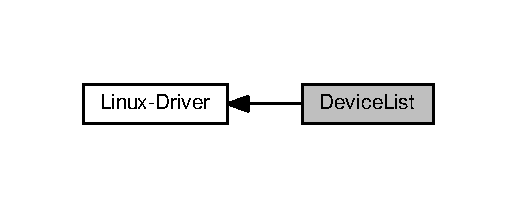
\includegraphics[width=248pt]{group___device_list}
\end{center}
\end{figure}
\subsection*{Strutture dati}
\begin{DoxyCompactItemize}
\item 
struct \hyperlink{structmy_g_p_i_o_k__list__t}{my\+G\+P\+I\+O\+K\+\_\+list\+\_\+t}
\begin{DoxyCompactList}\small\item\em Struttura dati per la gestione degli oggetti \hyperlink{structmy_g_p_i_o_k__t}{my\+G\+P\+I\+O\+K\+\_\+t} gestiti dal driver. \end{DoxyCompactList}\end{DoxyCompactItemize}
\subsection*{Funzioni}
\begin{DoxyCompactItemize}
\item 
int \hyperlink{group___device_list_ga1051095fc78c8ba7cf0b20a20fa253d2}{my\+G\+P\+I\+O\+K\+\_\+list\+\_\+\+Init} (\hyperlink{structmy_g_p_i_o_k__list__t}{my\+G\+P\+I\+O\+K\+\_\+list\+\_\+t} $\ast$list, uint32\+\_\+t list\+\_\+size)
\begin{DoxyCompactList}\small\item\em Inizializza una struttura dati \hyperlink{structmy_g_p_i_o_k__list__t}{my\+G\+P\+I\+O\+K\+\_\+list\+\_\+t}. \end{DoxyCompactList}\item 
void \hyperlink{group___device_list_ga416dfff8f4bf6034c87d60968056c621}{my\+G\+P\+I\+O\+K\+\_\+list\+\_\+\+Destroy} (\hyperlink{structmy_g_p_i_o_k__list__t}{my\+G\+P\+I\+O\+K\+\_\+list\+\_\+t} $\ast$list)
\begin{DoxyCompactList}\small\item\em Dealloca gli oggetti internamente gestiti da un oggetto \hyperlink{structmy_g_p_i_o_k__list__t}{my\+G\+P\+I\+O\+K\+\_\+list\+\_\+t}, liberando la memoria. \end{DoxyCompactList}\item 
int \hyperlink{group___device_list_gac5048cf2dbbbce3c39485e15595e88c9}{my\+G\+P\+I\+O\+K\+\_\+list\+\_\+add} (\hyperlink{structmy_g_p_i_o_k__list__t}{my\+G\+P\+I\+O\+K\+\_\+list\+\_\+t} $\ast$list, \hyperlink{structmy_g_p_i_o_k__t}{my\+G\+P\+I\+O\+K\+\_\+t} $\ast$device)
\begin{DoxyCompactList}\small\item\em Aggiunge un riferimento ad un oggetto \hyperlink{structmy_g_p_i_o_k__t}{my\+G\+P\+I\+O\+K\+\_\+t} alla lista. \end{DoxyCompactList}\item 
\hyperlink{structmy_g_p_i_o_k__t}{my\+G\+P\+I\+O\+K\+\_\+t} $\ast$ \hyperlink{group___device_list_ga616aa45c32b2ff391fc2b89930d1141b}{my\+G\+P\+I\+O\+K\+\_\+list\+\_\+find\+\_\+by\+\_\+op} (\hyperlink{structmy_g_p_i_o_k__list__t}{my\+G\+P\+I\+O\+K\+\_\+list\+\_\+t} $\ast$list, struct platform\+\_\+device $\ast$op)
\begin{DoxyCompactList}\small\item\em Ricerca un oggetto \hyperlink{structmy_g_p_i_o_k__t}{my\+G\+P\+I\+O\+K\+\_\+t} all'interno della lista. \end{DoxyCompactList}\item 
\hyperlink{structmy_g_p_i_o_k__t}{my\+G\+P\+I\+O\+K\+\_\+t} $\ast$ \hyperlink{group___device_list_gaf50b0da291040e8da5050194a4979849}{my\+G\+P\+I\+O\+K\+\_\+list\+\_\+find\+\_\+by\+\_\+minor} (\hyperlink{structmy_g_p_i_o_k__list__t}{my\+G\+P\+I\+O\+K\+\_\+list\+\_\+t} $\ast$list, dev\+\_\+t dev)
\begin{DoxyCompactList}\small\item\em Ricerca un oggetto \hyperlink{structmy_g_p_i_o_k__t}{my\+G\+P\+I\+O\+K\+\_\+t} all'interno della lista. \end{DoxyCompactList}\item 
\hyperlink{structmy_g_p_i_o_k__t}{my\+G\+P\+I\+O\+K\+\_\+t} $\ast$ \hyperlink{group___device_list_ga0bb70e18f51367d95fa28f723679ac30}{my\+G\+P\+I\+O\+K\+\_\+list\+\_\+find\+\_\+irq\+\_\+line} (\hyperlink{structmy_g_p_i_o_k__list__t}{my\+G\+P\+I\+O\+K\+\_\+list\+\_\+t} $\ast$list, int irq\+\_\+line)
\begin{DoxyCompactList}\small\item\em Ricerca un oggetto \hyperlink{structmy_g_p_i_o_k__t}{my\+G\+P\+I\+O\+K\+\_\+t} all'interno della lista. \end{DoxyCompactList}\item 
uint32\+\_\+t \hyperlink{group___device_list_ga731d5b5cbb96c6c5ef53936c23cdc58a}{my\+G\+P\+I\+O\+K\+\_\+list\+\_\+device\+\_\+count} (\hyperlink{structmy_g_p_i_o_k__list__t}{my\+G\+P\+I\+O\+K\+\_\+list\+\_\+t} $\ast$list)
\begin{DoxyCompactList}\small\item\em Restituisce il numero di device correntemente inseriti nella lista. \end{DoxyCompactList}\end{DoxyCompactItemize}


\subsection{Descrizione dettagliata}
Definisce la struttura dati \hyperlink{structmy_g_p_i_o_k__list__t}{my\+G\+P\+I\+O\+K\+\_\+list\+\_\+t}, la quale mantiene un riferimento agli oggetti \hyperlink{structmy_g_p_i_o_k__t}{my\+G\+P\+I\+O\+K\+\_\+t} gestiti dal driver. 



\subsection{Documentazione delle funzioni}
\hypertarget{group___device_list_gac5048cf2dbbbce3c39485e15595e88c9}{\index{Device\+List@{Device\+List}!my\+G\+P\+I\+O\+K\+\_\+list\+\_\+add@{my\+G\+P\+I\+O\+K\+\_\+list\+\_\+add}}
\index{my\+G\+P\+I\+O\+K\+\_\+list\+\_\+add@{my\+G\+P\+I\+O\+K\+\_\+list\+\_\+add}!Device\+List@{Device\+List}}
\subsubsection[{my\+G\+P\+I\+O\+K\+\_\+list\+\_\+add}]{\setlength{\rightskip}{0pt plus 5cm}int my\+G\+P\+I\+O\+K\+\_\+list\+\_\+add (
\begin{DoxyParamCaption}
\item[{{\bf my\+G\+P\+I\+O\+K\+\_\+list\+\_\+t} $\ast$}]{list, }
\item[{{\bf my\+G\+P\+I\+O\+K\+\_\+t} $\ast$}]{device}
\end{DoxyParamCaption}
)}}\label{group___device_list_gac5048cf2dbbbce3c39485e15595e88c9}


Aggiunge un riferimento ad un oggetto \hyperlink{structmy_g_p_i_o_k__t}{my\+G\+P\+I\+O\+K\+\_\+t} alla lista. 


\begin{DoxyParams}[1]{Parametri}
\mbox{\tt in}  & {\em list} & puntatore a \hyperlink{structmy_g_p_i_o_k__list__t}{my\+G\+P\+I\+O\+K\+\_\+list\+\_\+t}, lista a cui aggiungere l'oggetto \\
\hline
\mbox{\tt in}  & {\em device} & puntatore a \hyperlink{structmy_g_p_i_o_k__t}{my\+G\+P\+I\+O\+K\+\_\+t}, oggetto da aggiungere alla lista \\
\hline
\end{DoxyParams}

\begin{DoxyRetVals}{Valori di ritorno}
{\em -\/1} & se lo spazio si e' esaurito \\
\hline
{\em 0} & se non si manifesta nessun errore\\
\hline
\end{DoxyRetVals}
\begin{DoxyWarning}{Avvertimento}
La funzione si limita ad aggiungere l'oggetto \hyperlink{structmy_g_p_i_o_k__t}{my\+G\+P\+I\+O\+K\+\_\+t} alla lista, senza effettuare alcun tipo di controllo su di esso. Non viene verificato, ad esempio, se il device che si intende aggiungere sia effettivamente gia' presente in lista o se si tratti di un puntatore nullo. 
\end{DoxyWarning}
\hypertarget{group___device_list_ga416dfff8f4bf6034c87d60968056c621}{\index{Device\+List@{Device\+List}!my\+G\+P\+I\+O\+K\+\_\+list\+\_\+\+Destroy@{my\+G\+P\+I\+O\+K\+\_\+list\+\_\+\+Destroy}}
\index{my\+G\+P\+I\+O\+K\+\_\+list\+\_\+\+Destroy@{my\+G\+P\+I\+O\+K\+\_\+list\+\_\+\+Destroy}!Device\+List@{Device\+List}}
\subsubsection[{my\+G\+P\+I\+O\+K\+\_\+list\+\_\+\+Destroy}]{\setlength{\rightskip}{0pt plus 5cm}void my\+G\+P\+I\+O\+K\+\_\+list\+\_\+\+Destroy (
\begin{DoxyParamCaption}
\item[{{\bf my\+G\+P\+I\+O\+K\+\_\+list\+\_\+t} $\ast$}]{list}
\end{DoxyParamCaption}
)}}\label{group___device_list_ga416dfff8f4bf6034c87d60968056c621}


Dealloca gli oggetti internamente gestiti da un oggetto \hyperlink{structmy_g_p_i_o_k__list__t}{my\+G\+P\+I\+O\+K\+\_\+list\+\_\+t}, liberando la memoria. 


\begin{DoxyParams}[1]{Parametri}
\mbox{\tt in}  & {\em list} & puntatore a \hyperlink{structmy_g_p_i_o_k__list__t}{my\+G\+P\+I\+O\+K\+\_\+list\+\_\+t}, lista da distruggere \\
\hline
\end{DoxyParams}
\hypertarget{group___device_list_ga731d5b5cbb96c6c5ef53936c23cdc58a}{\index{Device\+List@{Device\+List}!my\+G\+P\+I\+O\+K\+\_\+list\+\_\+device\+\_\+count@{my\+G\+P\+I\+O\+K\+\_\+list\+\_\+device\+\_\+count}}
\index{my\+G\+P\+I\+O\+K\+\_\+list\+\_\+device\+\_\+count@{my\+G\+P\+I\+O\+K\+\_\+list\+\_\+device\+\_\+count}!Device\+List@{Device\+List}}
\subsubsection[{my\+G\+P\+I\+O\+K\+\_\+list\+\_\+device\+\_\+count}]{\setlength{\rightskip}{0pt plus 5cm}uint32\+\_\+t my\+G\+P\+I\+O\+K\+\_\+list\+\_\+device\+\_\+count (
\begin{DoxyParamCaption}
\item[{{\bf my\+G\+P\+I\+O\+K\+\_\+list\+\_\+t} $\ast$}]{list}
\end{DoxyParamCaption}
)}}\label{group___device_list_ga731d5b5cbb96c6c5ef53936c23cdc58a}


Restituisce il numero di device correntemente inseriti nella lista. 


\begin{DoxyParams}[1]{Parametri}
\mbox{\tt in}  & {\em list} & puntatore a \hyperlink{structmy_g_p_i_o_k__list__t}{my\+G\+P\+I\+O\+K\+\_\+list\+\_\+t}, lista di cui si intende conoscere il numero di oggetti \hyperlink{structmy_g_p_i_o_k__t}{my\+G\+P\+I\+O\+K\+\_\+t} contenuti \\
\hline
\end{DoxyParams}
\begin{DoxyReturn}{Restituisce}
numero di device correntemente inseriti nella lista 
\end{DoxyReturn}
\hypertarget{group___device_list_gaf50b0da291040e8da5050194a4979849}{\index{Device\+List@{Device\+List}!my\+G\+P\+I\+O\+K\+\_\+list\+\_\+find\+\_\+by\+\_\+minor@{my\+G\+P\+I\+O\+K\+\_\+list\+\_\+find\+\_\+by\+\_\+minor}}
\index{my\+G\+P\+I\+O\+K\+\_\+list\+\_\+find\+\_\+by\+\_\+minor@{my\+G\+P\+I\+O\+K\+\_\+list\+\_\+find\+\_\+by\+\_\+minor}!Device\+List@{Device\+List}}
\subsubsection[{my\+G\+P\+I\+O\+K\+\_\+list\+\_\+find\+\_\+by\+\_\+minor}]{\setlength{\rightskip}{0pt plus 5cm}{\bf my\+G\+P\+I\+O\+K\+\_\+t} $\ast$ my\+G\+P\+I\+O\+K\+\_\+list\+\_\+find\+\_\+by\+\_\+minor (
\begin{DoxyParamCaption}
\item[{{\bf my\+G\+P\+I\+O\+K\+\_\+list\+\_\+t} $\ast$}]{list, }
\item[{dev\+\_\+t}]{dev}
\end{DoxyParamCaption}
)}}\label{group___device_list_gaf50b0da291040e8da5050194a4979849}


Ricerca un oggetto \hyperlink{structmy_g_p_i_o_k__t}{my\+G\+P\+I\+O\+K\+\_\+t} all'interno della lista. 


\begin{DoxyParams}[1]{Parametri}
\mbox{\tt in}  & {\em list} & puntatore a \hyperlink{structmy_g_p_i_o_k__list__t}{my\+G\+P\+I\+O\+K\+\_\+list\+\_\+t}, lista in cui effettuare la ricerca \\
\hline
\mbox{\tt in}  & {\em dev} & major/minor number associato al device, parametro con cui viene invocata la open() o la release() \\
\hline
\end{DoxyParams}
\begin{DoxyReturn}{Restituisce}
indirizzo dell'oggetto \hyperlink{structmy_g_p_i_o_k__t}{my\+G\+P\+I\+O\+K\+\_\+t}, se e' presente nella lista, N\+U\+L\+L altrimenti 
\end{DoxyReturn}
\hypertarget{group___device_list_ga616aa45c32b2ff391fc2b89930d1141b}{\index{Device\+List@{Device\+List}!my\+G\+P\+I\+O\+K\+\_\+list\+\_\+find\+\_\+by\+\_\+op@{my\+G\+P\+I\+O\+K\+\_\+list\+\_\+find\+\_\+by\+\_\+op}}
\index{my\+G\+P\+I\+O\+K\+\_\+list\+\_\+find\+\_\+by\+\_\+op@{my\+G\+P\+I\+O\+K\+\_\+list\+\_\+find\+\_\+by\+\_\+op}!Device\+List@{Device\+List}}
\subsubsection[{my\+G\+P\+I\+O\+K\+\_\+list\+\_\+find\+\_\+by\+\_\+op}]{\setlength{\rightskip}{0pt plus 5cm}{\bf my\+G\+P\+I\+O\+K\+\_\+t} $\ast$ my\+G\+P\+I\+O\+K\+\_\+list\+\_\+find\+\_\+by\+\_\+op (
\begin{DoxyParamCaption}
\item[{{\bf my\+G\+P\+I\+O\+K\+\_\+list\+\_\+t} $\ast$}]{list, }
\item[{struct platform\+\_\+device $\ast$}]{op}
\end{DoxyParamCaption}
)}}\label{group___device_list_ga616aa45c32b2ff391fc2b89930d1141b}


Ricerca un oggetto \hyperlink{structmy_g_p_i_o_k__t}{my\+G\+P\+I\+O\+K\+\_\+t} all'interno della lista. 


\begin{DoxyParams}[1]{Parametri}
\mbox{\tt in}  & {\em list} & puntatore a \hyperlink{structmy_g_p_i_o_k__list__t}{my\+G\+P\+I\+O\+K\+\_\+list\+\_\+t}, lista in cui effettuare la ricerca \\
\hline
\mbox{\tt in}  & {\em op} & puntatore a struct platform\+\_\+device, argomento con cui viene invocata probe() o remove(), associato ad un oggetto \hyperlink{structmy_g_p_i_o_k__t}{my\+G\+P\+I\+O\+K\+\_\+t} \\
\hline
\end{DoxyParams}
\begin{DoxyReturn}{Restituisce}
indirizzo dell'oggetto \hyperlink{structmy_g_p_i_o_k__t}{my\+G\+P\+I\+O\+K\+\_\+t}, se e' presente nella lista, N\+U\+L\+L altrimenti 
\end{DoxyReturn}
\hypertarget{group___device_list_ga0bb70e18f51367d95fa28f723679ac30}{\index{Device\+List@{Device\+List}!my\+G\+P\+I\+O\+K\+\_\+list\+\_\+find\+\_\+irq\+\_\+line@{my\+G\+P\+I\+O\+K\+\_\+list\+\_\+find\+\_\+irq\+\_\+line}}
\index{my\+G\+P\+I\+O\+K\+\_\+list\+\_\+find\+\_\+irq\+\_\+line@{my\+G\+P\+I\+O\+K\+\_\+list\+\_\+find\+\_\+irq\+\_\+line}!Device\+List@{Device\+List}}
\subsubsection[{my\+G\+P\+I\+O\+K\+\_\+list\+\_\+find\+\_\+irq\+\_\+line}]{\setlength{\rightskip}{0pt plus 5cm}{\bf my\+G\+P\+I\+O\+K\+\_\+t} $\ast$ my\+G\+P\+I\+O\+K\+\_\+list\+\_\+find\+\_\+irq\+\_\+line (
\begin{DoxyParamCaption}
\item[{{\bf my\+G\+P\+I\+O\+K\+\_\+list\+\_\+t} $\ast$}]{list, }
\item[{int}]{irq\+\_\+line}
\end{DoxyParamCaption}
)}}\label{group___device_list_ga0bb70e18f51367d95fa28f723679ac30}


Ricerca un oggetto \hyperlink{structmy_g_p_i_o_k__t}{my\+G\+P\+I\+O\+K\+\_\+t} all'interno della lista. 


\begin{DoxyParams}[1]{Parametri}
\mbox{\tt in}  & {\em list} & puntatore a \hyperlink{structmy_g_p_i_o_k__list__t}{my\+G\+P\+I\+O\+K\+\_\+list\+\_\+t}, lista in cui effettuare la ricerca \\
\hline
 & {\em \mbox{[}in\mbox{[}} & irq\+\_\+line linea di interruzione alla quale il device e' connesso, parametro di invocazione della I\+S\+R \\
\hline
\end{DoxyParams}
\begin{DoxyReturn}{Restituisce}
indirizzo dell'oggetto \hyperlink{structmy_g_p_i_o_k__t}{my\+G\+P\+I\+O\+K\+\_\+t}, se e' presente nella lista, N\+U\+L\+L altrimenti 
\end{DoxyReturn}
\hypertarget{group___device_list_ga1051095fc78c8ba7cf0b20a20fa253d2}{\index{Device\+List@{Device\+List}!my\+G\+P\+I\+O\+K\+\_\+list\+\_\+\+Init@{my\+G\+P\+I\+O\+K\+\_\+list\+\_\+\+Init}}
\index{my\+G\+P\+I\+O\+K\+\_\+list\+\_\+\+Init@{my\+G\+P\+I\+O\+K\+\_\+list\+\_\+\+Init}!Device\+List@{Device\+List}}
\subsubsection[{my\+G\+P\+I\+O\+K\+\_\+list\+\_\+\+Init}]{\setlength{\rightskip}{0pt plus 5cm}int my\+G\+P\+I\+O\+K\+\_\+list\+\_\+\+Init (
\begin{DoxyParamCaption}
\item[{{\bf my\+G\+P\+I\+O\+K\+\_\+list\+\_\+t} $\ast$}]{list, }
\item[{uint32\+\_\+t}]{list\+\_\+size}
\end{DoxyParamCaption}
)}}\label{group___device_list_ga1051095fc78c8ba7cf0b20a20fa253d2}


Inizializza una struttura dati \hyperlink{structmy_g_p_i_o_k__list__t}{my\+G\+P\+I\+O\+K\+\_\+list\+\_\+t}. 


\begin{DoxyParams}[1]{Parametri}
\mbox{\tt in}  & {\em list} & puntatore a \hyperlink{structmy_g_p_i_o_k__list__t}{my\+G\+P\+I\+O\+K\+\_\+list\+\_\+t}, lista da inizializzare \\
\hline
\mbox{\tt in}  & {\em list\+\_\+size} & numero massimo di device che la struttra dati potra' gestire \\
\hline
\end{DoxyParams}

\begin{DoxyRetVals}{Valori di ritorno}
{\em -\/\+E\+N\+O\+M\+E\+M} & nel caso in cui la struttura non possa essere allocata in memoria \\
\hline
{\em 0} & se non si manifestano errori \\
\hline
\end{DoxyRetVals}

\hypertarget{group__my_g_p_i_o_k__t}{}\section{My\+G\+P\+I\+O\+K\+\_\+t}
\label{group__my_g_p_i_o_k__t}\index{My\+G\+P\+I\+O\+K\+\_\+t@{My\+G\+P\+I\+O\+K\+\_\+t}}


Definisce l\textquotesingle{}oggetto \hyperlink{structmy_g_p_i_o_k__t}{my\+G\+P\+I\+O\+K\+\_\+t}, che rappresenta un device my\+G\+P\+IO a livello kernel.  


Diagramma di collaborazione per My\+G\+P\+I\+O\+K\+\_\+t\+:\nopagebreak
\begin{figure}[H]
\begin{center}
\leavevmode
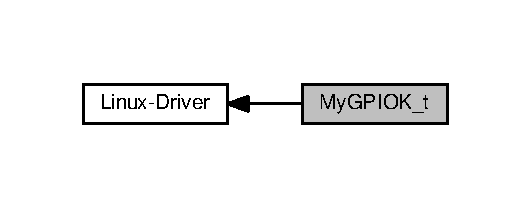
\includegraphics[width=255pt]{group__my_g_p_i_o_k__t}
\end{center}
\end{figure}
\subsection*{Strutture dati}
\begin{DoxyCompactItemize}
\item 
struct \hyperlink{structmy_g_p_i_o_k__t}{my\+G\+P\+I\+O\+K\+\_\+t}
\begin{DoxyCompactList}\small\item\em Stuttura per l\textquotesingle{}astrazione di un device my\+G\+P\+IO in kernel-\/mode. \end{DoxyCompactList}\end{DoxyCompactItemize}
\subsection*{Definizioni}
\begin{DoxyCompactItemize}
\item 
\#define \hyperlink{group__my_g_p_i_o_k__t_ga0da2526ca3cd1a94ebcecf96778ea2e5}{my\+G\+P\+I\+O\+K\+\_\+\+G\+I\+E\+S\+\_\+\+O\+F\+F\+S\+ET}~0x0\+CU
\begin{DoxyCompactList}\small\item\em Offset, rispetto all\textquotesingle{}indirizzo base, del registro \char`\"{}\+G\+I\+E\+S\char`\"{}. \end{DoxyCompactList}\item 
\#define \hyperlink{group__my_g_p_i_o_k__t_ga2ed7646e6f910f5803477e51b7fe26e3}{my\+G\+P\+I\+O\+K\+\_\+\+P\+I\+E\+\_\+\+O\+F\+F\+S\+ET}~0x10U
\begin{DoxyCompactList}\small\item\em Offset, rispetto all\textquotesingle{}indirizzo base, del registro \char`\"{}\+P\+I\+E\char`\"{}. \end{DoxyCompactList}\item 
\#define \hyperlink{group__my_g_p_i_o_k__t_ga37ee502d1ba364dfde9261c4f7a537a6}{my\+G\+P\+I\+O\+K\+\_\+\+I\+R\+Q\+\_\+\+O\+F\+F\+S\+ET}~0x14U
\begin{DoxyCompactList}\small\item\em Offset, rispetto all\textquotesingle{}indirizzo base, del registro \char`\"{}\+I\+R\+Q\char`\"{}. \end{DoxyCompactList}\item 
\#define \hyperlink{group__my_g_p_i_o_k__t_gac72408c288009c213c0231973b3fe761}{my\+G\+P\+I\+O\+K\+\_\+\+I\+A\+C\+K\+\_\+\+O\+F\+F\+S\+ET}~0x18U
\begin{DoxyCompactList}\small\item\em Offset, rispetto all\textquotesingle{}indirizzo base, del registro \char`\"{}\+I\+A\+C\+K\char`\"{}. \end{DoxyCompactList}\end{DoxyCompactItemize}
\subsection*{Funzioni}
\begin{DoxyCompactItemize}
\item 
int \hyperlink{group__my_g_p_i_o_k__t_ga64afb2eff1f990814d792349842c522d}{my\+G\+P\+I\+O\+K\+\_\+\+Init} (\hyperlink{structmy_g_p_i_o_k__t}{my\+G\+P\+I\+O\+K\+\_\+t} $\ast$my\+G\+P\+I\+O\+K\+\_\+device, struct module $\ast$owner, struct platform\+\_\+device $\ast$op, struct class $\ast$class, const char $\ast$driver\+\_\+name, const char $\ast$device\+\_\+name, uint32\+\_\+t serial, struct file\+\_\+operations $\ast$f\+\_\+ops, irq\+\_\+handler\+\_\+t irq\+\_\+handler, uint32\+\_\+t irq\+\_\+mask)
\begin{DoxyCompactList}\small\item\em Inizializza una struttura \hyperlink{structmy_g_p_i_o_k__t}{my\+G\+P\+I\+O\+K\+\_\+t} e configura il device corrispondente. \end{DoxyCompactList}\item 
void \hyperlink{group__my_g_p_i_o_k__t_ga24255b79dd8549aa655cf28c1f9a65d5}{my\+G\+P\+I\+O\+K\+\_\+\+Destroy} (\hyperlink{structmy_g_p_i_o_k__t}{my\+G\+P\+I\+O\+K\+\_\+t} $\ast$device)
\begin{DoxyCompactList}\small\item\em Deinizializza un device, rimuovendo le strutture kernel allocate per il suo funzionamento. \end{DoxyCompactList}\item 
void \hyperlink{group__my_g_p_i_o_k__t_gad82c1051e6acb335b1b26ab0c459453b}{my\+G\+P\+I\+O\+K\+\_\+\+Set\+Can\+Read} (\hyperlink{structmy_g_p_i_o_k__t}{my\+G\+P\+I\+O\+K\+\_\+t} $\ast$device)
\begin{DoxyCompactList}\small\item\em Set del flag \char`\"{}interrupt occurred\char`\"{} (can\+Read) \end{DoxyCompactList}\item 
void \hyperlink{group__my_g_p_i_o_k__t_ga6dc0ec06b388522ffc524e5fd14d8b72}{my\+G\+P\+I\+O\+K\+\_\+\+Reset\+Can\+Read} (\hyperlink{structmy_g_p_i_o_k__t}{my\+G\+P\+I\+O\+K\+\_\+t} $\ast$device)
\begin{DoxyCompactList}\small\item\em Reset del flag \char`\"{}interrupt occurred\char`\"{} (can\+Read) \end{DoxyCompactList}\item 
void \hyperlink{group__my_g_p_i_o_k__t_gaf1b6f35c097c46361d675a42f122828e}{my\+G\+P\+I\+O\+K\+\_\+\+Test\+Can\+Read\+And\+Sleep} (\hyperlink{structmy_g_p_i_o_k__t}{my\+G\+P\+I\+O\+K\+\_\+t} $\ast$device)
\begin{DoxyCompactList}\small\item\em Testa la condizione \char`\"{}interrupt occurred\char`\"{}, mettendo in attesa il processo, se necessario. \end{DoxyCompactList}\item 
unsigned \hyperlink{group__my_g_p_i_o_k__t_gae428f50a6da69e3cf89348b8ba9401b1}{my\+G\+P\+I\+O\+K\+\_\+\+Get\+Poll\+Mask} (\hyperlink{structmy_g_p_i_o_k__t}{my\+G\+P\+I\+O\+K\+\_\+t} $\ast$device, struct file $\ast$file\+\_\+ptr, struct poll\+\_\+table\+\_\+struct $\ast$wait)
\begin{DoxyCompactList}\small\item\em Verifica che le operazioni di lettura/scrittura risultino non-\/bloccanti. \end{DoxyCompactList}\item 
void \hyperlink{group__my_g_p_i_o_k__t_ga5a7df448de9de94620ce1baf7ec388c9}{my\+G\+P\+I\+O\+K\+\_\+\+Increment\+Total} (\hyperlink{structmy_g_p_i_o_k__t}{my\+G\+P\+I\+O\+K\+\_\+t} $\ast$device)
\begin{DoxyCompactList}\small\item\em Incrementa il contatore degli interrupt per un particolare device. \end{DoxyCompactList}\item 
void \hyperlink{group__my_g_p_i_o_k__t_gae182aa943af08c102a05795ae8526192}{my\+G\+P\+I\+O\+K\+\_\+\+Wake\+Up} (\hyperlink{structmy_g_p_i_o_k__t}{my\+G\+P\+I\+O\+K\+\_\+t} $\ast$device)
\begin{DoxyCompactList}\small\item\em Risveglia i process in attesa sulle code di read e poll. \end{DoxyCompactList}\item 
void $\ast$ \hyperlink{group__my_g_p_i_o_k__t_ga565ffd4946b330b29e1166dfc9851b11}{my\+G\+P\+I\+O\+K\+\_\+\+Get\+Device\+Address} (\hyperlink{structmy_g_p_i_o_k__t}{my\+G\+P\+I\+O\+K\+\_\+t} $\ast$device)
\begin{DoxyCompactList}\small\item\em Restituisce l\textquotesingle{}indirizzo virtuale di memoria cui è mappato un device. \end{DoxyCompactList}\item 
void \hyperlink{group__my_g_p_i_o_k__t_ga00a24f28b49c71aaa91f66be71a3895b}{my\+G\+P\+I\+O\+K\+\_\+\+Global\+Interrupt\+Enable} (\hyperlink{structmy_g_p_i_o_k__t}{my\+G\+P\+I\+O\+K\+\_\+t} $\ast$my\+G\+P\+I\+O\+K\+\_\+device)
\begin{DoxyCompactList}\small\item\em Abilita gli interrupt globali;. \end{DoxyCompactList}\item 
void \hyperlink{group__my_g_p_i_o_k__t_gace0d81f5ec65978f22118a3f1fc8b222}{my\+G\+P\+I\+O\+K\+\_\+\+Global\+Interrupt\+Disable} (\hyperlink{structmy_g_p_i_o_k__t}{my\+G\+P\+I\+O\+K\+\_\+t} $\ast$my\+G\+P\+I\+O\+K\+\_\+device)
\begin{DoxyCompactList}\small\item\em Disabilita gli interrupt globali;. \end{DoxyCompactList}\item 
void \hyperlink{group__my_g_p_i_o_k__t_ga179c20f5f62e8ce1593cbedff2f00533}{my\+G\+P\+I\+O\+K\+\_\+\+Pin\+Interrupt\+Enable} (\hyperlink{structmy_g_p_i_o_k__t}{my\+G\+P\+I\+O\+K\+\_\+t} $\ast$my\+G\+P\+I\+O\+K\+\_\+device, unsigned mask)
\begin{DoxyCompactList}\small\item\em Abilita gli interrupt per i singoli pin del device. \end{DoxyCompactList}\item 
void \hyperlink{group__my_g_p_i_o_k__t_gabfd91641f98a4725aec779c8834ca92d}{my\+G\+P\+I\+O\+K\+\_\+\+Pin\+Interrupt\+Disable} (\hyperlink{structmy_g_p_i_o_k__t}{my\+G\+P\+I\+O\+K\+\_\+t} $\ast$my\+G\+P\+I\+O\+K\+\_\+device, unsigned mask)
\begin{DoxyCompactList}\small\item\em Disabilita gli interrupt per i singoli pin del device. \end{DoxyCompactList}\item 
unsigned \hyperlink{group__my_g_p_i_o_k__t_ga1b3ad44b9198f537493180d748de0b6c}{my\+G\+P\+I\+O\+K\+\_\+\+Pending\+Pin\+Interrupt} (\hyperlink{structmy_g_p_i_o_k__t}{my\+G\+P\+I\+O\+K\+\_\+t} $\ast$my\+G\+P\+I\+O\+K\+\_\+device)
\begin{DoxyCompactList}\small\item\em Consente di ottenere una maschera che indichi quali interrupt non siano stati ancora serviti;. \end{DoxyCompactList}\item 
void \hyperlink{group__my_g_p_i_o_k__t_ga8eaf8f1b21aa6f772c395faf457144f9}{my\+G\+P\+I\+O\+K\+\_\+\+Pin\+Interrupt\+Ack} (\hyperlink{structmy_g_p_i_o_k__t}{my\+G\+P\+I\+O\+K\+\_\+t} $\ast$my\+G\+P\+I\+O\+K\+\_\+device, unsigned mask)
\begin{DoxyCompactList}\small\item\em Invia al device notifica di servizio di un interrupt;. \end{DoxyCompactList}\end{DoxyCompactItemize}


\subsection{Descrizione dettagliata}
Definisce l\textquotesingle{}oggetto \hyperlink{structmy_g_p_i_o_k__t}{my\+G\+P\+I\+O\+K\+\_\+t}, che rappresenta un device my\+G\+P\+IO a livello kernel. 



\subsection{Documentazione delle definizioni}
\mbox{\Hypertarget{group__my_g_p_i_o_k__t_ga0da2526ca3cd1a94ebcecf96778ea2e5}\label{group__my_g_p_i_o_k__t_ga0da2526ca3cd1a94ebcecf96778ea2e5}} 
\index{My\+G\+P\+I\+O\+K\+\_\+t@{My\+G\+P\+I\+O\+K\+\_\+t}!my\+G\+P\+I\+O\+K\+\_\+\+G\+I\+E\+S\+\_\+\+O\+F\+F\+S\+ET@{my\+G\+P\+I\+O\+K\+\_\+\+G\+I\+E\+S\+\_\+\+O\+F\+F\+S\+ET}}
\index{my\+G\+P\+I\+O\+K\+\_\+\+G\+I\+E\+S\+\_\+\+O\+F\+F\+S\+ET@{my\+G\+P\+I\+O\+K\+\_\+\+G\+I\+E\+S\+\_\+\+O\+F\+F\+S\+ET}!My\+G\+P\+I\+O\+K\+\_\+t@{My\+G\+P\+I\+O\+K\+\_\+t}}
\subsubsection{\texorpdfstring{my\+G\+P\+I\+O\+K\+\_\+\+G\+I\+E\+S\+\_\+\+O\+F\+F\+S\+ET}{myGPIOK\_GIES\_OFFSET}}
{\footnotesize\ttfamily \#define my\+G\+P\+I\+O\+K\+\_\+\+G\+I\+E\+S\+\_\+\+O\+F\+F\+S\+ET~0x0\+CU}



Offset, rispetto all\textquotesingle{}indirizzo base, del registro \char`\"{}\+G\+I\+E\+S\char`\"{}. 

\mbox{\Hypertarget{group__my_g_p_i_o_k__t_gac72408c288009c213c0231973b3fe761}\label{group__my_g_p_i_o_k__t_gac72408c288009c213c0231973b3fe761}} 
\index{My\+G\+P\+I\+O\+K\+\_\+t@{My\+G\+P\+I\+O\+K\+\_\+t}!my\+G\+P\+I\+O\+K\+\_\+\+I\+A\+C\+K\+\_\+\+O\+F\+F\+S\+ET@{my\+G\+P\+I\+O\+K\+\_\+\+I\+A\+C\+K\+\_\+\+O\+F\+F\+S\+ET}}
\index{my\+G\+P\+I\+O\+K\+\_\+\+I\+A\+C\+K\+\_\+\+O\+F\+F\+S\+ET@{my\+G\+P\+I\+O\+K\+\_\+\+I\+A\+C\+K\+\_\+\+O\+F\+F\+S\+ET}!My\+G\+P\+I\+O\+K\+\_\+t@{My\+G\+P\+I\+O\+K\+\_\+t}}
\subsubsection{\texorpdfstring{my\+G\+P\+I\+O\+K\+\_\+\+I\+A\+C\+K\+\_\+\+O\+F\+F\+S\+ET}{myGPIOK\_IACK\_OFFSET}}
{\footnotesize\ttfamily \#define my\+G\+P\+I\+O\+K\+\_\+\+I\+A\+C\+K\+\_\+\+O\+F\+F\+S\+ET~0x18U}



Offset, rispetto all\textquotesingle{}indirizzo base, del registro \char`\"{}\+I\+A\+C\+K\char`\"{}. 

\mbox{\Hypertarget{group__my_g_p_i_o_k__t_ga37ee502d1ba364dfde9261c4f7a537a6}\label{group__my_g_p_i_o_k__t_ga37ee502d1ba364dfde9261c4f7a537a6}} 
\index{My\+G\+P\+I\+O\+K\+\_\+t@{My\+G\+P\+I\+O\+K\+\_\+t}!my\+G\+P\+I\+O\+K\+\_\+\+I\+R\+Q\+\_\+\+O\+F\+F\+S\+ET@{my\+G\+P\+I\+O\+K\+\_\+\+I\+R\+Q\+\_\+\+O\+F\+F\+S\+ET}}
\index{my\+G\+P\+I\+O\+K\+\_\+\+I\+R\+Q\+\_\+\+O\+F\+F\+S\+ET@{my\+G\+P\+I\+O\+K\+\_\+\+I\+R\+Q\+\_\+\+O\+F\+F\+S\+ET}!My\+G\+P\+I\+O\+K\+\_\+t@{My\+G\+P\+I\+O\+K\+\_\+t}}
\subsubsection{\texorpdfstring{my\+G\+P\+I\+O\+K\+\_\+\+I\+R\+Q\+\_\+\+O\+F\+F\+S\+ET}{myGPIOK\_IRQ\_OFFSET}}
{\footnotesize\ttfamily \#define my\+G\+P\+I\+O\+K\+\_\+\+I\+R\+Q\+\_\+\+O\+F\+F\+S\+ET~0x14U}



Offset, rispetto all\textquotesingle{}indirizzo base, del registro \char`\"{}\+I\+R\+Q\char`\"{}. 

\mbox{\Hypertarget{group__my_g_p_i_o_k__t_ga2ed7646e6f910f5803477e51b7fe26e3}\label{group__my_g_p_i_o_k__t_ga2ed7646e6f910f5803477e51b7fe26e3}} 
\index{My\+G\+P\+I\+O\+K\+\_\+t@{My\+G\+P\+I\+O\+K\+\_\+t}!my\+G\+P\+I\+O\+K\+\_\+\+P\+I\+E\+\_\+\+O\+F\+F\+S\+ET@{my\+G\+P\+I\+O\+K\+\_\+\+P\+I\+E\+\_\+\+O\+F\+F\+S\+ET}}
\index{my\+G\+P\+I\+O\+K\+\_\+\+P\+I\+E\+\_\+\+O\+F\+F\+S\+ET@{my\+G\+P\+I\+O\+K\+\_\+\+P\+I\+E\+\_\+\+O\+F\+F\+S\+ET}!My\+G\+P\+I\+O\+K\+\_\+t@{My\+G\+P\+I\+O\+K\+\_\+t}}
\subsubsection{\texorpdfstring{my\+G\+P\+I\+O\+K\+\_\+\+P\+I\+E\+\_\+\+O\+F\+F\+S\+ET}{myGPIOK\_PIE\_OFFSET}}
{\footnotesize\ttfamily \#define my\+G\+P\+I\+O\+K\+\_\+\+P\+I\+E\+\_\+\+O\+F\+F\+S\+ET~0x10U}



Offset, rispetto all\textquotesingle{}indirizzo base, del registro \char`\"{}\+P\+I\+E\char`\"{}. 



\subsection{Documentazione delle funzioni}
\mbox{\Hypertarget{group__my_g_p_i_o_k__t_ga24255b79dd8549aa655cf28c1f9a65d5}\label{group__my_g_p_i_o_k__t_ga24255b79dd8549aa655cf28c1f9a65d5}} 
\index{My\+G\+P\+I\+O\+K\+\_\+t@{My\+G\+P\+I\+O\+K\+\_\+t}!my\+G\+P\+I\+O\+K\+\_\+\+Destroy@{my\+G\+P\+I\+O\+K\+\_\+\+Destroy}}
\index{my\+G\+P\+I\+O\+K\+\_\+\+Destroy@{my\+G\+P\+I\+O\+K\+\_\+\+Destroy}!My\+G\+P\+I\+O\+K\+\_\+t@{My\+G\+P\+I\+O\+K\+\_\+t}}
\subsubsection{\texorpdfstring{my\+G\+P\+I\+O\+K\+\_\+\+Destroy()}{myGPIOK\_Destroy()}}
{\footnotesize\ttfamily void my\+G\+P\+I\+O\+K\+\_\+\+Destroy (\begin{DoxyParamCaption}\item[{\hyperlink{structmy_g_p_i_o_k__t}{my\+G\+P\+I\+O\+K\+\_\+t} $\ast$}]{device }\end{DoxyParamCaption})}



Deinizializza un device, rimuovendo le strutture kernel allocate per il suo funzionamento. 


\begin{DoxyParams}[1]{Parametri}
\mbox{\tt in}  & {\em device} & puntatore a struttura \hyperlink{structmy_g_p_i_o_k__t}{my\+G\+P\+I\+O\+K\+\_\+t}, specifica il particolare device su cui agire \\
\hline
\end{DoxyParams}
\mbox{\Hypertarget{group__my_g_p_i_o_k__t_ga565ffd4946b330b29e1166dfc9851b11}\label{group__my_g_p_i_o_k__t_ga565ffd4946b330b29e1166dfc9851b11}} 
\index{My\+G\+P\+I\+O\+K\+\_\+t@{My\+G\+P\+I\+O\+K\+\_\+t}!my\+G\+P\+I\+O\+K\+\_\+\+Get\+Device\+Address@{my\+G\+P\+I\+O\+K\+\_\+\+Get\+Device\+Address}}
\index{my\+G\+P\+I\+O\+K\+\_\+\+Get\+Device\+Address@{my\+G\+P\+I\+O\+K\+\_\+\+Get\+Device\+Address}!My\+G\+P\+I\+O\+K\+\_\+t@{My\+G\+P\+I\+O\+K\+\_\+t}}
\subsubsection{\texorpdfstring{my\+G\+P\+I\+O\+K\+\_\+\+Get\+Device\+Address()}{myGPIOK\_GetDeviceAddress()}}
{\footnotesize\ttfamily void$\ast$ my\+G\+P\+I\+O\+K\+\_\+\+Get\+Device\+Address (\begin{DoxyParamCaption}\item[{\hyperlink{structmy_g_p_i_o_k__t}{my\+G\+P\+I\+O\+K\+\_\+t} $\ast$}]{device }\end{DoxyParamCaption})}



Restituisce l\textquotesingle{}indirizzo virtuale di memoria cui è mappato un device. 


\begin{DoxyParams}[1]{Parametri}
\mbox{\tt in}  & {\em device} & puntatore a struttura \hyperlink{structmy_g_p_i_o_k__t}{my\+G\+P\+I\+O\+K\+\_\+t}, che si riferisce al device su cui operare \\
\hline
\end{DoxyParams}
\mbox{\Hypertarget{group__my_g_p_i_o_k__t_gae428f50a6da69e3cf89348b8ba9401b1}\label{group__my_g_p_i_o_k__t_gae428f50a6da69e3cf89348b8ba9401b1}} 
\index{My\+G\+P\+I\+O\+K\+\_\+t@{My\+G\+P\+I\+O\+K\+\_\+t}!my\+G\+P\+I\+O\+K\+\_\+\+Get\+Poll\+Mask@{my\+G\+P\+I\+O\+K\+\_\+\+Get\+Poll\+Mask}}
\index{my\+G\+P\+I\+O\+K\+\_\+\+Get\+Poll\+Mask@{my\+G\+P\+I\+O\+K\+\_\+\+Get\+Poll\+Mask}!My\+G\+P\+I\+O\+K\+\_\+t@{My\+G\+P\+I\+O\+K\+\_\+t}}
\subsubsection{\texorpdfstring{my\+G\+P\+I\+O\+K\+\_\+\+Get\+Poll\+Mask()}{myGPIOK\_GetPollMask()}}
{\footnotesize\ttfamily unsigned my\+G\+P\+I\+O\+K\+\_\+\+Get\+Poll\+Mask (\begin{DoxyParamCaption}\item[{\hyperlink{structmy_g_p_i_o_k__t}{my\+G\+P\+I\+O\+K\+\_\+t} $\ast$}]{device,  }\item[{struct file $\ast$}]{file\+\_\+ptr,  }\item[{struct poll\+\_\+table\+\_\+struct $\ast$}]{wait }\end{DoxyParamCaption})}



Verifica che le operazioni di lettura/scrittura risultino non-\/bloccanti. 


\begin{DoxyParams}[1]{Parametri}
\mbox{\tt in}  & {\em device} & puntatore a struttura \hyperlink{structmy_g_p_i_o_k__t}{my\+G\+P\+I\+O\+K\+\_\+t}, che si riferisce al device su cui operare \\
\hline
\mbox{\tt in,out}  & {\em file} & \\
\hline
\mbox{\tt in,out}  & {\em wait} & \\
\hline
\end{DoxyParams}
\begin{DoxyReturn}{Restituisce}
restituisce una maschera di bit che indica se sia possibile effettuare operazioni di lettura/scrittura non bloccanti, in modo che il kernel possa bloccare il processo e risvegliarlo solo quando tali operazioni diventino possibili.
\end{DoxyReturn}
Questo metodo è il back-\/end di tre diverse system-\/calls\+: poll, epoll e select, le quali sono usate per capire se una operazione di lettura/scrittura du un device possano risultare bloccanti o meno. \mbox{\Hypertarget{group__my_g_p_i_o_k__t_gace0d81f5ec65978f22118a3f1fc8b222}\label{group__my_g_p_i_o_k__t_gace0d81f5ec65978f22118a3f1fc8b222}} 
\index{My\+G\+P\+I\+O\+K\+\_\+t@{My\+G\+P\+I\+O\+K\+\_\+t}!my\+G\+P\+I\+O\+K\+\_\+\+Global\+Interrupt\+Disable@{my\+G\+P\+I\+O\+K\+\_\+\+Global\+Interrupt\+Disable}}
\index{my\+G\+P\+I\+O\+K\+\_\+\+Global\+Interrupt\+Disable@{my\+G\+P\+I\+O\+K\+\_\+\+Global\+Interrupt\+Disable}!My\+G\+P\+I\+O\+K\+\_\+t@{My\+G\+P\+I\+O\+K\+\_\+t}}
\subsubsection{\texorpdfstring{my\+G\+P\+I\+O\+K\+\_\+\+Global\+Interrupt\+Disable()}{myGPIOK\_GlobalInterruptDisable()}}
{\footnotesize\ttfamily void my\+G\+P\+I\+O\+K\+\_\+\+Global\+Interrupt\+Disable (\begin{DoxyParamCaption}\item[{\hyperlink{structmy_g_p_i_o_k__t}{my\+G\+P\+I\+O\+K\+\_\+t} $\ast$}]{device }\end{DoxyParamCaption})}



Disabilita gli interrupt globali;. 


\begin{DoxyParams}[1]{Parametri}
\mbox{\tt in}  & {\em device} & puntatore a struttura \hyperlink{structmy_g_p_i_o_k__t}{my\+G\+P\+I\+O\+K\+\_\+t}, che si riferisce al device su cui operare \\
\hline
\end{DoxyParams}
\mbox{\Hypertarget{group__my_g_p_i_o_k__t_ga00a24f28b49c71aaa91f66be71a3895b}\label{group__my_g_p_i_o_k__t_ga00a24f28b49c71aaa91f66be71a3895b}} 
\index{My\+G\+P\+I\+O\+K\+\_\+t@{My\+G\+P\+I\+O\+K\+\_\+t}!my\+G\+P\+I\+O\+K\+\_\+\+Global\+Interrupt\+Enable@{my\+G\+P\+I\+O\+K\+\_\+\+Global\+Interrupt\+Enable}}
\index{my\+G\+P\+I\+O\+K\+\_\+\+Global\+Interrupt\+Enable@{my\+G\+P\+I\+O\+K\+\_\+\+Global\+Interrupt\+Enable}!My\+G\+P\+I\+O\+K\+\_\+t@{My\+G\+P\+I\+O\+K\+\_\+t}}
\subsubsection{\texorpdfstring{my\+G\+P\+I\+O\+K\+\_\+\+Global\+Interrupt\+Enable()}{myGPIOK\_GlobalInterruptEnable()}}
{\footnotesize\ttfamily void my\+G\+P\+I\+O\+K\+\_\+\+Global\+Interrupt\+Enable (\begin{DoxyParamCaption}\item[{\hyperlink{structmy_g_p_i_o_k__t}{my\+G\+P\+I\+O\+K\+\_\+t} $\ast$}]{device }\end{DoxyParamCaption})}



Abilita gli interrupt globali;. 


\begin{DoxyParams}[1]{Parametri}
\mbox{\tt in}  & {\em device} & puntatore a struttura \hyperlink{structmy_g_p_i_o_k__t}{my\+G\+P\+I\+O\+K\+\_\+t}, che si riferisce al device su cui operare \\
\hline
\end{DoxyParams}
\mbox{\Hypertarget{group__my_g_p_i_o_k__t_ga5a7df448de9de94620ce1baf7ec388c9}\label{group__my_g_p_i_o_k__t_ga5a7df448de9de94620ce1baf7ec388c9}} 
\index{My\+G\+P\+I\+O\+K\+\_\+t@{My\+G\+P\+I\+O\+K\+\_\+t}!my\+G\+P\+I\+O\+K\+\_\+\+Increment\+Total@{my\+G\+P\+I\+O\+K\+\_\+\+Increment\+Total}}
\index{my\+G\+P\+I\+O\+K\+\_\+\+Increment\+Total@{my\+G\+P\+I\+O\+K\+\_\+\+Increment\+Total}!My\+G\+P\+I\+O\+K\+\_\+t@{My\+G\+P\+I\+O\+K\+\_\+t}}
\subsubsection{\texorpdfstring{my\+G\+P\+I\+O\+K\+\_\+\+Increment\+Total()}{myGPIOK\_IncrementTotal()}}
{\footnotesize\ttfamily void my\+G\+P\+I\+O\+K\+\_\+\+Increment\+Total (\begin{DoxyParamCaption}\item[{\hyperlink{structmy_g_p_i_o_k__t}{my\+G\+P\+I\+O\+K\+\_\+t} $\ast$}]{device }\end{DoxyParamCaption})}



Incrementa il contatore degli interrupt per un particolare device. 


\begin{DoxyParams}[1]{Parametri}
\mbox{\tt in}  & {\em device} & puntatore a struttura \hyperlink{structmy_g_p_i_o_k__t}{my\+G\+P\+I\+O\+K\+\_\+t}, che si riferisce al device su cui operare\\
\hline
\end{DoxyParams}
\subparagraph*{Incremento del numero totale di interrupt}

Dopo aver settato il flag, viene incrementato il valore degli interrupt totali. Anche questa operazione viene effettuata in mutua esclusione. \mbox{\Hypertarget{group__my_g_p_i_o_k__t_ga64afb2eff1f990814d792349842c522d}\label{group__my_g_p_i_o_k__t_ga64afb2eff1f990814d792349842c522d}} 
\index{My\+G\+P\+I\+O\+K\+\_\+t@{My\+G\+P\+I\+O\+K\+\_\+t}!my\+G\+P\+I\+O\+K\+\_\+\+Init@{my\+G\+P\+I\+O\+K\+\_\+\+Init}}
\index{my\+G\+P\+I\+O\+K\+\_\+\+Init@{my\+G\+P\+I\+O\+K\+\_\+\+Init}!My\+G\+P\+I\+O\+K\+\_\+t@{My\+G\+P\+I\+O\+K\+\_\+t}}
\subsubsection{\texorpdfstring{my\+G\+P\+I\+O\+K\+\_\+\+Init()}{myGPIOK\_Init()}}
{\footnotesize\ttfamily int my\+G\+P\+I\+O\+K\+\_\+\+Init (\begin{DoxyParamCaption}\item[{\hyperlink{structmy_g_p_i_o_k__t}{my\+G\+P\+I\+O\+K\+\_\+t} $\ast$}]{my\+G\+P\+I\+O\+K\+\_\+device,  }\item[{struct module $\ast$}]{owner,  }\item[{struct platform\+\_\+device $\ast$}]{op,  }\item[{struct class $\ast$}]{class,  }\item[{const char $\ast$}]{driver\+\_\+name,  }\item[{const char $\ast$}]{device\+\_\+name,  }\item[{uint32\+\_\+t}]{serial,  }\item[{struct file\+\_\+operations $\ast$}]{f\+\_\+ops,  }\item[{irq\+\_\+handler\+\_\+t}]{irq\+\_\+handler,  }\item[{uint32\+\_\+t}]{irq\+\_\+mask }\end{DoxyParamCaption})}



Inizializza una struttura \hyperlink{structmy_g_p_i_o_k__t}{my\+G\+P\+I\+O\+K\+\_\+t} e configura il device corrispondente. 


\begin{DoxyParams}[1]{Parametri}
\mbox{\tt in}  & {\em my\+G\+P\+I\+O\+K\+\_\+device} & puntatore a struttura \hyperlink{structmy_g_p_i_o_k__t}{my\+G\+P\+I\+O\+K\+\_\+t}, che si riferisce al device su cui operare \\
\hline
\mbox{\tt in}  & {\em owner} & puntatore a struttura struct module, proprietario del device (T\+H\+I\+S\+\_\+\+M\+O\+D\+U\+LE) \\
\hline
\mbox{\tt in}  & {\em op} & puntatore a struct platform\+\_\+device, costituito dal parametro \char`\"{}op\char`\"{} con cui viene invocata probe() o la remove() \\
\hline
\mbox{\tt in}  & {\em class} & puntatore a struct class, classe del device, deve essere stata precedentemente creata con class\+\_\+create() \\
\hline
\mbox{\tt in}  & {\em driver\+\_\+name} & nome del driver \\
\hline
\mbox{\tt in}  & {\em device\+\_\+name} & nome del device \\
\hline
\mbox{\tt in}  & {\em serial} & numero seriale del device \\
\hline
\mbox{\tt in}  & {\em f\+\_\+ops} & puntatore a struttura struct file\+\_\+operations, specifica le funzioni che agiscono sul device \\
\hline
\mbox{\tt in}  & {\em irq\+\_\+handler} & puntatore irq\+\_\+handler\+\_\+t alla funzione che gestirà gli interrupt generati dal device \\
\hline
\mbox{\tt in}  & {\em irq\+\_\+mask} & maschera delle interruzioni del device\\
\hline
\end{DoxyParams}

\begin{DoxyRetVals}{Valori di ritorno}
{\em 0} & se non si è verificato nessun errore \\
\hline
\end{DoxyRetVals}
\subparagraph*{Major-\/number e Minor-\/number}

Ai device drivers sono associati un major-\/number ed un minor-\/number. Il major-\/number viene usato dal kernel per identificare il driver corretto corrispondente ad uno specifico device, quando si effettuano operazioni su di esso. Il ruolo del minor number dipende dal device e viene gestito internamente dal driver. Questo driver, così come molti altri, usa il Major ed il minor number per distinguere le diverse istanze di device my\+G\+P\+IO che usano il device-\/driver my\+G\+P\+I\+OK. La registrazione di un device driver può essere effettuata chiamando {\bfseries alloc\+\_\+chrdev\+\_\+region()}, la quale alloca un char-\/device numbers. Il major number viene scelto dinamicamente e restituito dalla funzione attraverso il parametro dev. La funzione restituisce un valore negativo nel caso in cui si verifichino errori, 0 altrimenti. 
\begin{DoxyCode}
\textcolor{keywordtype}{int} alloc\_chrdev\_region (dev\_t * dev, \textcolor{keywordtype}{unsigned} baseminor, \textcolor{keywordtype}{unsigned} count, \textcolor{keyword}{const} \textcolor{keywordtype}{char} *name);
\end{DoxyCode}

\begin{DoxyItemize}
\item dev\+: major e minor number
\item baseminor\+: primo dei minor number richiesti
\item count\+: numero di minornumber richiesti
\item name\+: nome del device
\end{DoxyItemize}

\subparagraph*{Operatori}

Essendo un device \char`\"{}visto\char`\"{} come un file, ogni device driver deve implementare tutte le system-\/call previste per l\textquotesingle{}interfacciamento con un file. La corrispondenza tra la system-\/call e la funzione fornita dal driver viene stabilita attraverso la struttura file\+\_\+operations. La struttura dati file\+\_\+operations, definita in $<$linux/fs.\+h$>$ mantiene puntatori a funzioni definite dal driver che consentono di definire il comportamento degli operatori che agiscono su un file. 
\begin{DoxyCode}
\textcolor{keyword}{static} \textcolor{keyword}{struct }file\_operations myGPIO\_fops = \{
    .owner      = THIS\_MODULE,
    .llseek     = driver\_seek,
    .read       = driver\_read,
    .write      = driver\_write,
    .poll       = driver\_poll,
    .open       = driver\_open,
    .release    = driver\_release
\};
\end{DoxyCode}
 Ogni campo della struttura deve puntare ad una funzione del driver che implementa uno specifico \char`\"{}operatore\char`\"{} su file, oppure impostata a N\+U\+LL se l\textquotesingle{}operatore non è supportato. L\textquotesingle{}esatto comportamento del kernel, quando uno dei puntatori è N\+U\+LL, varia da funzione a funzione. La lista seguente introduce tutti gli operatori che un\textquotesingle{}applicazione può invocare su un device. La lista è stata mantenuta snella, includendo solo i campi strettamente necessari.


\begin{DoxyItemize}
\item {\itshape struct module $\ast$owner} \+:~\newline
 il primo campo della struttura non è un operatore, ma un puntatore al modulo che \char`\"{}possiede\char`\"{} la struttura. Il campo ha lo scopo di evitare che il modulo venga rimosso dal kernel quando uno degli operatori è in uso. Viene inizializzato usando la macro T\+H\+I\+S\+\_\+\+M\+O\+D\+U\+LE, definita in $<$linux/module.\+h$>$.
\item {\itshape loff\+\_\+t ($\ast$llseek) (struct file $\ast$, loff\+\_\+t, int)} \+: il campo llseek è usato per cambiare la posizione della \char`\"{}testina\char`\"{} di lettura/ scrittura in un file. La funzione restituisce la nuova posizione della testina. loff\+\_\+t è un intero a 64 bit (anche su architetture a 32 bit). Eventuali errori vengono segnalati con un valore di ritorno negativo. Se questo campo è posto a N\+U\+LL, eventuali chiamate a seek modifigheranno la posizione della testina in un modo impredicibile.
\item {\itshape ssize\+\_\+t ($\ast$read) (struct file $\ast$, char \+\_\+ \+\_\+user $\ast$, size\+\_\+t, loff\+\_\+t $\ast$)} \+:~\newline
 usata per leggere dati dal device. Se lasciato a N\+U\+LL, ogni chiamata a read fallirà e non sarà possibile leggere dal device. La funzione restituisce il numero di byte letti con successo ma, nel caso si verifichi un errore, restituisce un numero intero negativo.
\item {\itshape ssize\+\_\+t ($\ast$write) (struct file $\ast$, const char \+\_\+ \+\_\+user $\ast$, size\+\_\+t, loff\+\_\+t $\ast$)} \+:~\newline
 invia dati al device. Se N\+U\+LL ogni chiamata alla system-\/call write causerà un errore. Il valore di ritorno, se non negativo, rappresenta il numero di byte correttamente scritti.
\item {\itshape unsigned int ($\ast$poll) (struct file $\ast$, struct poll\+\_\+table\+\_\+struct $\ast$)} \+:~\newline
 questo metodo è il back-\/end di tre diverse system-\/calls\+: poll, epoll e select, le quali sono usate per capire se una operazione di lettura/scrittura du un device possano risultare bloccanti o meno. La funzione dovrebbe restituire una maschera che indichi se sia possibile effettuare operazioni di lettura/scrittura non bloccanti, in modo che il kernel possa bloccare il processo e risvegliarlo solo quando tali operazioni diventino possibili. Se viene lasciata N\+U\+LL si intende che le operazioni di lettura/scrittura sul device siano sempre non-\/bloccanti.
\item {\itshape int ($\ast$open) (struct inode $\ast$, struct file $\ast$)} \+:~\newline
 Anche se, di solito, è la prima operazione che si effettua su un file, non è strettamente necessaria la sua implementazione. Se lasciata N\+U\+LL, l\textquotesingle{}apertura del device andrà comunque a buon fine, ma al driver non verrà inviata alcuna notifica.
\item {\itshape int ($\ast$release) (struct inode $\ast$, struct file $\ast$)} \+:~\newline
 questo operatore viene invocato quando il file viene rilasciato. Come open, può essere lasciato N\+U\+LL.
\end{DoxyItemize}

L\textquotesingle{}inizializzazione di un device a caratteri passa anche attraverso la definizione di questo tipo di operatori. Essi possono essere impostati attraverso l\textquotesingle{}uso della funzione 
\begin{DoxyCode}
\textcolor{keywordtype}{void} cdev\_init (\textcolor{keyword}{struct} cdev *cdev, \textcolor{keyword}{const} \textcolor{keyword}{struct} file\_operations *fops);
\end{DoxyCode}
 la quale prende, come parametri
\begin{DoxyItemize}
\item cdev\+: puntatore a struttura cdev da inizializzare;
\item fops\+: puntatore a struttura file\+\_\+operation con cui inizializzare il device.
\end{DoxyItemize}

\subparagraph*{Creazione del device}

Il passo successivo è la registrazione del device e la sua aggiunta al filesystem. Tale operazione può essere effettuata chiamando 
\begin{DoxyCode}
\textcolor{keyword}{struct }device * device\_create( \textcolor{keyword}{struct} \textcolor{keyword}{class} *\textcolor{keyword}{class}, \textcolor{keyword}{struct} device *parent, dev\_t devt, \textcolor{keyword}{const} \textcolor{keywordtype}{char} *fmt, ...
      )
\end{DoxyCode}

\begin{DoxyItemize}
\item class\+: puntatore alla struttura class alla quale il device deve essere registrato
\item parent\+: puntatore ad eventuale device parent
\item devt\+: tmajor number
\item fmt\+: nome del device.
\end{DoxyItemize}

La funzione pù essere usata solo sulla classe dei device a caratteri. Crea un device all\textquotesingle{}interno del filesystem, associandogli il major number preventivamente inizializzato. La funzione restituisce il puntatore alla struttura device creata all\textquotesingle{}interno del filesystem. Si noti che il puntatre alla struttura classes D\+E\+VE essere stato precedentemente creato attraverso una chiamata alla funzione {\itshape class\+\_\+create()}.

\subparagraph*{Aggiunta del device}

Il driver, a questo punto, è pronto per essere aggiunto. è possibile aggiungere il driver usando 
\begin{DoxyCode}
\textcolor{keywordtype}{int} cdev\_add (\textcolor{keyword}{struct} cdev *p, dev\_t dev, \textcolor{keywordtype}{unsigned} count);
\end{DoxyCode}
 La quale accetta come parametri
\begin{DoxyItemize}
\item p\+: puntatore a struttura cdev structure per il device
\item dev\+: device number (precedentemente inizializzato usando la funzione {\itshape alloc\+\_\+chrdev\+\_\+region()})
\item count\+: numero di minor-\/numbers richiesti per il device
\end{DoxyItemize}

La funzione restituisce un numero negativo in caso di errore.

\subparagraph*{Accedere al segmento di memoria a cui la periferica è mappata}

Un driver, tipicamente, prende possesso del segmento di memoria cui è mappato il device con la funzione di probe. Il problema è che il device è mappato ad un indirizzo di memoria fisico ed il Kernel, così come qualsiasi altro programma, lavora su indirizzi di memoria virtuali. La funzione


\begin{DoxyCode}
\textcolor{keywordtype}{int} of\_address\_to\_resource(\textcolor{keyword}{struct} device\_node *node, \textcolor{keywordtype}{int} index, \textcolor{keyword}{struct} resource *r);
\end{DoxyCode}


popola una struttura resource con l\textquotesingle{}indirizzo di memoria cui è mapato il device usando le informazioni contenute all\textquotesingle{}interno del device tree. Ad esempio, se il device tree contiene 
\begin{DoxyCode}
reg = <0x41200000 0x10000>;
\end{DoxyCode}
 signidifa che l\textquotesingle{}indirizzo fisico associato al device è l\textquotesingle{}indirizzo 0x41200000, che al device sono riservati 0x10000 bytes. of\+\_\+address\+\_\+to\+\_\+resource() setterà res.\+start = 0x41200000 e res.\+end = 0x4120ffff.

\subparagraph*{Allocazione della memoria del device}

Le regioni di memoria per di I/O vanno allocate prima di poter essere usate. 
\begin{DoxyCode}
\textcolor{keyword}{struct }resource *request\_mem\_region(\textcolor{keywordtype}{unsigned} \textcolor{keywordtype}{long} start, \textcolor{keywordtype}{unsigned} \textcolor{keywordtype}{long} len, \textcolor{keywordtype}{char} *name);
\end{DoxyCode}
 Questa funzione alloca una regione di memoria di len byte a partire da start restituendone l\textquotesingle{}indirizzo, mentre nel caso in cui si verifichi un errore viene restituito N\+U\+LL. La funzione viene chiamata per ottenere l\textquotesingle{}accesso esclusivo della regione di memoria, per evitare che driver diversi tentino di accedere allo stesso spazio di memoria.

\subparagraph*{Remapping}

L\textquotesingle{}allocazione dello spazio di memoria non è l\textquotesingle{}unico step da eseguire prima che tale memoria possa essere usata. è necessario fare in modo che sia resa accessibile al kernel attraverso un mapping, usando la funzione. 
\begin{DoxyCode}
\textcolor{keywordtype}{void} *ioremap(\textcolor{keywordtype}{unsigned} \textcolor{keywordtype}{long} phys\_addr, \textcolor{keywordtype}{unsigned} \textcolor{keywordtype}{long} size);
\end{DoxyCode}


\subparagraph*{Registrazione di un interrupt-\/handler}

Il modulo deve registrare un handler per gli interrupt. L\textquotesingle{}handler deve essere compatibile con il tipo puntatore a funzione irq\+\_\+handler\+\_\+t, così definito. 
\begin{DoxyCode}
\textcolor{keyword}{struct }irqreturn\_t (*irq\_handler\_t)(\textcolor{keywordtype}{int} irq, \textcolor{keyword}{struct} pt\_regs * regs);
\end{DoxyCode}
 Il modulo definisce la funzione \hyperlink{group___linux-_driver_ga2fc230a12a97aa63e43b2dc4aec73511}{my\+G\+P\+I\+O\+K\+\_\+irq\+\_\+handler()}. L\textquotesingle{}handler può essere registrato usando 
\begin{DoxyCode}
\textcolor{keywordtype}{int} request\_irq(    \textcolor{keywordtype}{unsigned} \textcolor{keywordtype}{int} irqNumber,
                    irqreturn\_t (*handler)(\textcolor{keywordtype}{int}, \textcolor{keywordtype}{void} *, \textcolor{keyword}{struct} pt\_regs *),
                    \textcolor{keywordtype}{unsigned} \textcolor{keywordtype}{long} irqflags,
                    \textcolor{keyword}{const} \textcolor{keywordtype}{char} *devname,
                    \textcolor{keywordtype}{void} *dev\_id);
\end{DoxyCode}
 Il parametro irq\+Number può essere determinato automaticamente usando la funzione 
\begin{DoxyCode}
\textcolor{keywordtype}{unsigned} \textcolor{keywordtype}{int} irq\_of\_parse\_and\_map(\textcolor{keyword}{struct} device\_node *node, \textcolor{keywordtype}{int} index);
\end{DoxyCode}
 Il parametro ($\ast$handler) è il puntatore alla funzione interrupt-\/handler, mentre il parametro irq flags è una maschera di bit, il cui valore può essere impostato con uno dei flag I\+R\+Q\+F\+\_\+ definiti in $<$linux/interrupt.\+h$>$. In questo caso nessuno di tali flag viene usato, motivo per cui il parametro viene posto a zero.

La funzione irq\+\_\+of\+\_\+parse\+\_\+and\+\_\+map() effettua un looks-\/up nella specifica degli interrupt all\textquotesingle{}interno del device tree e restituisce un irq number così come de lo aspetta request\+\_\+irq() (cioè compaci con l\textquotesingle{}enumerazione in /proc/interrupts). Il secondo argomento della funzione è, tipicamente, zero, ad indicare che, all\textquotesingle{}interno del device tree, verrà preso in considerazione soltanto il primo degli interrupt specificate. Il device tree, nella sezione dedicata al gpio,reca 
\begin{DoxyCode}
interrupts = <0 29 4>;
\end{DoxyCode}
 Il primo numero (0) è un flag che indica se l\textquotesingle{}interrupt sia connesso ad una line S\+PI (shared peripheral interrupt). Un valore diverso da zero indica che la linea è S\+PI. Il secondo numero si riferisce all\textquotesingle{}interrupt number. Per farla breve, quando si definisce la parte hardware, in questo specifico esempio il device G\+P\+IO è connesso alla linea 61 del G\+IC. Sottraendo 32 si orriene 29. Il terzo numero si riferisce alla tipologia dell\textquotesingle{}interrupt. Sono possibili tre valori\+:
\begin{DoxyItemize}
\item 0 \+: power-\/up default
\item 1 \+: rising-\/edge
\item 4 \+: a livelli, active alto
\end{DoxyItemize}

\subparagraph*{Inizializzazione della wait-\/queue per la system-\/call read() e poll()}

In linux una wait queue viene implementata da una struttura dati wait\+\_\+queue\+\_\+head\+\_\+t, definita in $<$linux/wait.\+h$>$. Il driver in questione prevede due wait-\/queue differenti\+: una per la system-\/call read() ed una per la system-\/call poll(). Entrambe le code vengono inizializzate dalla funzione \hyperlink{group___linux-_driver_gae40973a06d72f7c41a9af07513a62307}{my\+G\+P\+I\+O\+K\+\_\+probe()}. 
\begin{DoxyCode}
init\_waitqueue\_head(&my\_queue);
\end{DoxyCode}
 Si veda la documentazione della funzione \hyperlink{group___linux-_driver_ga90ac339df9c02ae5f11a2a7727adc923}{my\+G\+P\+I\+O\+K\+\_\+read()} per dettagli ulteriori.

\subparagraph*{Inizializzazione degli spinlock}

I semafori sono uno strumento potentissimo per per l\textquotesingle{}implementazione di sezioni critiche, ma non possono essere usati in codice non interrompibile. Gli spilock sono come i semafori, ma possono essere usati anche in codice non interrompibile, come può esserlo un modulo kernel. Sostanzialmente se uno spinlock è già stato acquisito da qualcun altro, si entra in un hot-\/loop dal quale si esce solo quando chi possiede lo spinlock lo rilascia. Trattandosi di moduli kernel, è di vitale importanza che la sezione critica sia quanto più piccola possibile. Ovviamente l\textquotesingle{}implementazione è \char`\"{}un pò\char`\"{} più complessa di come è stata descritta, ma il concetto è questo. Gli spinlock sono definiti in $<$linux/spinlock.\+h$>$. L\textquotesingle{}inizializzazione di uno spinlock avviene usando la funzione 
\begin{DoxyCode}
\textcolor{keywordtype}{void} spin\_lock\_init(spinlock\_t *lock);
\end{DoxyCode}


\subparagraph*{Abilitazione degli interrupt del device}

A seconda del valore C\+F\+L\+A\+G\+S\+\_\+my\+G\+P\+I\+O\+K.\+o (si veda il Makefile a corredo), vengono abilitati gli interrupt della periferica. Se si tratta del G\+P\+IO Xilinx vengono abilitati gli interrupt globali e gli interrupt sul canale due. Se si tratta del device G\+P\+IO custom, essendo esso parecchio più semplice, è necessario abilitare solo gli interrupt globali.\mbox{\Hypertarget{group__my_g_p_i_o_k__t_ga1b3ad44b9198f537493180d748de0b6c}\label{group__my_g_p_i_o_k__t_ga1b3ad44b9198f537493180d748de0b6c}} 
\index{My\+G\+P\+I\+O\+K\+\_\+t@{My\+G\+P\+I\+O\+K\+\_\+t}!my\+G\+P\+I\+O\+K\+\_\+\+Pending\+Pin\+Interrupt@{my\+G\+P\+I\+O\+K\+\_\+\+Pending\+Pin\+Interrupt}}
\index{my\+G\+P\+I\+O\+K\+\_\+\+Pending\+Pin\+Interrupt@{my\+G\+P\+I\+O\+K\+\_\+\+Pending\+Pin\+Interrupt}!My\+G\+P\+I\+O\+K\+\_\+t@{My\+G\+P\+I\+O\+K\+\_\+t}}
\subsubsection{\texorpdfstring{my\+G\+P\+I\+O\+K\+\_\+\+Pending\+Pin\+Interrupt()}{myGPIOK\_PendingPinInterrupt()}}
{\footnotesize\ttfamily unsigned my\+G\+P\+I\+O\+K\+\_\+\+Pending\+Pin\+Interrupt (\begin{DoxyParamCaption}\item[{\hyperlink{structmy_g_p_i_o_k__t}{my\+G\+P\+I\+O\+K\+\_\+t} $\ast$}]{device }\end{DoxyParamCaption})}



Consente di ottenere una maschera che indichi quali interrupt non siano stati ancora serviti;. 


\begin{DoxyParams}[1]{Parametri}
\mbox{\tt in}  & {\em device} & puntatore a struttura \hyperlink{structmy_g_p_i_o_k__t}{my\+G\+P\+I\+O\+K\+\_\+t}, che si riferisce al device su cui operare\\
\hline
\end{DoxyParams}
\begin{DoxyReturn}{Restituisce}
maschera che riporta i pin per i quali gli interrupt non sono stati ancora serviti; 
\end{DoxyReturn}
\mbox{\Hypertarget{group__my_g_p_i_o_k__t_ga8eaf8f1b21aa6f772c395faf457144f9}\label{group__my_g_p_i_o_k__t_ga8eaf8f1b21aa6f772c395faf457144f9}} 
\index{My\+G\+P\+I\+O\+K\+\_\+t@{My\+G\+P\+I\+O\+K\+\_\+t}!my\+G\+P\+I\+O\+K\+\_\+\+Pin\+Interrupt\+Ack@{my\+G\+P\+I\+O\+K\+\_\+\+Pin\+Interrupt\+Ack}}
\index{my\+G\+P\+I\+O\+K\+\_\+\+Pin\+Interrupt\+Ack@{my\+G\+P\+I\+O\+K\+\_\+\+Pin\+Interrupt\+Ack}!My\+G\+P\+I\+O\+K\+\_\+t@{My\+G\+P\+I\+O\+K\+\_\+t}}
\subsubsection{\texorpdfstring{my\+G\+P\+I\+O\+K\+\_\+\+Pin\+Interrupt\+Ack()}{myGPIOK\_PinInterruptAck()}}
{\footnotesize\ttfamily void my\+G\+P\+I\+O\+K\+\_\+\+Pin\+Interrupt\+Ack (\begin{DoxyParamCaption}\item[{\hyperlink{structmy_g_p_i_o_k__t}{my\+G\+P\+I\+O\+K\+\_\+t} $\ast$}]{device,  }\item[{unsigned}]{mask }\end{DoxyParamCaption})}



Invia al device notifica di servizio di un interrupt;. 


\begin{DoxyParams}[1]{Parametri}
\mbox{\tt in}  & {\em device} & puntatore a struttura \hyperlink{structmy_g_p_i_o_k__t}{my\+G\+P\+I\+O\+K\+\_\+t}, che si riferisce al device su cui operare\\
\hline
\mbox{\tt in}  & {\em mask} & mask maschera di selezione degli interrupt da notificare; quelli non selezionati non vengono notificati; \\
\hline
\end{DoxyParams}
\mbox{\Hypertarget{group__my_g_p_i_o_k__t_gabfd91641f98a4725aec779c8834ca92d}\label{group__my_g_p_i_o_k__t_gabfd91641f98a4725aec779c8834ca92d}} 
\index{My\+G\+P\+I\+O\+K\+\_\+t@{My\+G\+P\+I\+O\+K\+\_\+t}!my\+G\+P\+I\+O\+K\+\_\+\+Pin\+Interrupt\+Disable@{my\+G\+P\+I\+O\+K\+\_\+\+Pin\+Interrupt\+Disable}}
\index{my\+G\+P\+I\+O\+K\+\_\+\+Pin\+Interrupt\+Disable@{my\+G\+P\+I\+O\+K\+\_\+\+Pin\+Interrupt\+Disable}!My\+G\+P\+I\+O\+K\+\_\+t@{My\+G\+P\+I\+O\+K\+\_\+t}}
\subsubsection{\texorpdfstring{my\+G\+P\+I\+O\+K\+\_\+\+Pin\+Interrupt\+Disable()}{myGPIOK\_PinInterruptDisable()}}
{\footnotesize\ttfamily void my\+G\+P\+I\+O\+K\+\_\+\+Pin\+Interrupt\+Disable (\begin{DoxyParamCaption}\item[{\hyperlink{structmy_g_p_i_o_k__t}{my\+G\+P\+I\+O\+K\+\_\+t} $\ast$}]{device,  }\item[{unsigned}]{mask }\end{DoxyParamCaption})}



Disabilita gli interrupt per i singoli pin del device. 


\begin{DoxyParams}[1]{Parametri}
\mbox{\tt in}  & {\em device} & puntatore a struttura \hyperlink{structmy_g_p_i_o_k__t}{my\+G\+P\+I\+O\+K\+\_\+t}, che si riferisce al device su cui operare\\
\hline
\mbox{\tt in}  & {\em mask} & maschera di selezione degli interrupt da disabilitare; quelli non selezionati non vengono disabilitati; \\
\hline
\end{DoxyParams}
\mbox{\Hypertarget{group__my_g_p_i_o_k__t_ga179c20f5f62e8ce1593cbedff2f00533}\label{group__my_g_p_i_o_k__t_ga179c20f5f62e8ce1593cbedff2f00533}} 
\index{My\+G\+P\+I\+O\+K\+\_\+t@{My\+G\+P\+I\+O\+K\+\_\+t}!my\+G\+P\+I\+O\+K\+\_\+\+Pin\+Interrupt\+Enable@{my\+G\+P\+I\+O\+K\+\_\+\+Pin\+Interrupt\+Enable}}
\index{my\+G\+P\+I\+O\+K\+\_\+\+Pin\+Interrupt\+Enable@{my\+G\+P\+I\+O\+K\+\_\+\+Pin\+Interrupt\+Enable}!My\+G\+P\+I\+O\+K\+\_\+t@{My\+G\+P\+I\+O\+K\+\_\+t}}
\subsubsection{\texorpdfstring{my\+G\+P\+I\+O\+K\+\_\+\+Pin\+Interrupt\+Enable()}{myGPIOK\_PinInterruptEnable()}}
{\footnotesize\ttfamily void my\+G\+P\+I\+O\+K\+\_\+\+Pin\+Interrupt\+Enable (\begin{DoxyParamCaption}\item[{\hyperlink{structmy_g_p_i_o_k__t}{my\+G\+P\+I\+O\+K\+\_\+t} $\ast$}]{device,  }\item[{unsigned}]{mask }\end{DoxyParamCaption})}



Abilita gli interrupt per i singoli pin del device. 


\begin{DoxyParams}[1]{Parametri}
\mbox{\tt in}  & {\em device} & puntatore a struttura \hyperlink{structmy_g_p_i_o_k__t}{my\+G\+P\+I\+O\+K\+\_\+t}, che si riferisce al device su cui operare \\
\hline
\mbox{\tt in}  & {\em mask} & maschera di selezione degli interrupt da abilitare; quelli non selezionati non vengono abilitati; \\
\hline
\end{DoxyParams}
\mbox{\Hypertarget{group__my_g_p_i_o_k__t_ga6dc0ec06b388522ffc524e5fd14d8b72}\label{group__my_g_p_i_o_k__t_ga6dc0ec06b388522ffc524e5fd14d8b72}} 
\index{My\+G\+P\+I\+O\+K\+\_\+t@{My\+G\+P\+I\+O\+K\+\_\+t}!my\+G\+P\+I\+O\+K\+\_\+\+Reset\+Can\+Read@{my\+G\+P\+I\+O\+K\+\_\+\+Reset\+Can\+Read}}
\index{my\+G\+P\+I\+O\+K\+\_\+\+Reset\+Can\+Read@{my\+G\+P\+I\+O\+K\+\_\+\+Reset\+Can\+Read}!My\+G\+P\+I\+O\+K\+\_\+t@{My\+G\+P\+I\+O\+K\+\_\+t}}
\subsubsection{\texorpdfstring{my\+G\+P\+I\+O\+K\+\_\+\+Reset\+Can\+Read()}{myGPIOK\_ResetCanRead()}}
{\footnotesize\ttfamily void my\+G\+P\+I\+O\+K\+\_\+\+Reset\+Can\+Read (\begin{DoxyParamCaption}\item[{\hyperlink{structmy_g_p_i_o_k__t}{my\+G\+P\+I\+O\+K\+\_\+t} $\ast$}]{device }\end{DoxyParamCaption})}



Reset del flag \char`\"{}interrupt occurred\char`\"{} (can\+Read) 


\begin{DoxyParams}[1]{Parametri}
\mbox{\tt in}  & {\em device} & puntatore a struttura \hyperlink{structmy_g_p_i_o_k__t}{my\+G\+P\+I\+O\+K\+\_\+t}, che si riferisce al device su cui operare\\
\hline
\end{DoxyParams}
\subparagraph*{Reset del flag \char`\"{}interrupt occurred\char`\"{} per read() bloccanti}

Nel momento in cui il processo viene risvegliato e la condizione della quale era in attesa è tale che esso può continuare la sua esecuzione, è necessario resettare tale flag. Questa operazione va effettuata per prevenire race-\/condition dovute al risveglio di più processi in attesa del manifestarsi dello stesso evento. Il reset del flag va, pertanto, effettuato in mutua esclusione.

I semafori sono uno strumento potentissimo per per l\textquotesingle{}implementazione di sezioni critiche, ma non possono essere usati in codice non interrompibile. Gli spilock sono come i semafori, ma possono essere usati anche in codice non interrompibile, come può esserlo un modulo kernel. Sostanzialmente se uno spinlock è già stato acquisito da qualcun altro, si entra in un hot-\/loop dal quale si esce solo quando chi possiede lo spinlock lo rilascia. Trattandosi di moduli kernel, è di vitale importanza che la sezione critica sia quanto più piccola possibile. Ovviamente l\textquotesingle{}implementazione è \char`\"{}un pò\char`\"{} più complessa di come è stata descritta, ma il concetto è questo. Gli spinlock sono definiti in $<$linux/spinlock.\+h$>$. Esistono diversi modi per acquisire uno spinlock. Nel seguito viene usata la funzione 
\begin{DoxyCode}
\textcolor{keywordtype}{void} spin\_lock(spinlock\_t *lock);
\end{DoxyCode}
 per rilasciare uno spinlock, invece, verrà usata 
\begin{DoxyCode}
\textcolor{keywordtype}{void} spin\_unlock(spinlock\_t *lock);
\end{DoxyCode}
 \mbox{\Hypertarget{group__my_g_p_i_o_k__t_gad82c1051e6acb335b1b26ab0c459453b}\label{group__my_g_p_i_o_k__t_gad82c1051e6acb335b1b26ab0c459453b}} 
\index{My\+G\+P\+I\+O\+K\+\_\+t@{My\+G\+P\+I\+O\+K\+\_\+t}!my\+G\+P\+I\+O\+K\+\_\+\+Set\+Can\+Read@{my\+G\+P\+I\+O\+K\+\_\+\+Set\+Can\+Read}}
\index{my\+G\+P\+I\+O\+K\+\_\+\+Set\+Can\+Read@{my\+G\+P\+I\+O\+K\+\_\+\+Set\+Can\+Read}!My\+G\+P\+I\+O\+K\+\_\+t@{My\+G\+P\+I\+O\+K\+\_\+t}}
\subsubsection{\texorpdfstring{my\+G\+P\+I\+O\+K\+\_\+\+Set\+Can\+Read()}{myGPIOK\_SetCanRead()}}
{\footnotesize\ttfamily void my\+G\+P\+I\+O\+K\+\_\+\+Set\+Can\+Read (\begin{DoxyParamCaption}\item[{\hyperlink{structmy_g_p_i_o_k__t}{my\+G\+P\+I\+O\+K\+\_\+t} $\ast$}]{device }\end{DoxyParamCaption})}



Set del flag \char`\"{}interrupt occurred\char`\"{} (can\+Read) 


\begin{DoxyParams}[1]{Parametri}
\mbox{\tt in}  & {\em device} & puntatore a struttura \hyperlink{structmy_g_p_i_o_k__t}{my\+G\+P\+I\+O\+K\+\_\+t}, che si riferisce al device su cui operare\\
\hline
\end{DoxyParams}
\subparagraph*{Setting del valore del flag \char`\"{}interrupt occurred\char`\"{}}

Dopo aver disabilitato gli interrupt della periferica, occorre settare in modo appropriato il flag \char`\"{}interrupt occurred\char`\"{}, in modo che i processi in attesa possano essere risvegliati in modo sicuro. Per prevenire race condition, tale operazione viene effettuata mutua esclusione. I semafori sono uno strumento potentissimo per per l\textquotesingle{}implementazione di sezioni critiche, ma non possono essere usati in codice non interrompibile. Gli spilock sono come i semafori, ma possono essere usati anche in codice non interrompibile, come può esserlo un modulo kernel. Sostanzialmente se uno spinlock è già stato acquisito da qualcun altro, si entra in un hot-\/loop dal quale si esce solo quando chi possiede lo spinlock lo rilascia. Trattandosi di moduli kernel, è di vitale importanza che la sezione critica sia quanto più piccola possibile. Ovviamente l\textquotesingle{}implementazione è \char`\"{}un pò\char`\"{} più complessa di come è stata descritta, ma il concetto è questo. Gli spinlock sono definiti in $<$linux/spinlock.\+h$>$. Esistono diversi modi per acquisire uno spinlock. Nel seguito viene usata la funzione 
\begin{DoxyCode}
\textcolor{keywordtype}{void} spin\_lock\_irqsave(spinlock\_t *lock, \textcolor{keywordtype}{unsigned} \textcolor{keywordtype}{long} flags);
\end{DoxyCode}
 la quale disabilita gli interrupt sul processore locale prima di acquisire lo spinlock, per poi ripristinarlo quando lo spinlock viene rilasciato, usando 
\begin{DoxyCode}
\textcolor{keywordtype}{void} spin\_unlock\_irqrestore(spinlock\_t *lock, \textcolor{keywordtype}{unsigned} \textcolor{keywordtype}{long} flags);
\end{DoxyCode}
 \mbox{\Hypertarget{group__my_g_p_i_o_k__t_gaf1b6f35c097c46361d675a42f122828e}\label{group__my_g_p_i_o_k__t_gaf1b6f35c097c46361d675a42f122828e}} 
\index{My\+G\+P\+I\+O\+K\+\_\+t@{My\+G\+P\+I\+O\+K\+\_\+t}!my\+G\+P\+I\+O\+K\+\_\+\+Test\+Can\+Read\+And\+Sleep@{my\+G\+P\+I\+O\+K\+\_\+\+Test\+Can\+Read\+And\+Sleep}}
\index{my\+G\+P\+I\+O\+K\+\_\+\+Test\+Can\+Read\+And\+Sleep@{my\+G\+P\+I\+O\+K\+\_\+\+Test\+Can\+Read\+And\+Sleep}!My\+G\+P\+I\+O\+K\+\_\+t@{My\+G\+P\+I\+O\+K\+\_\+t}}
\subsubsection{\texorpdfstring{my\+G\+P\+I\+O\+K\+\_\+\+Test\+Can\+Read\+And\+Sleep()}{myGPIOK\_TestCanReadAndSleep()}}
{\footnotesize\ttfamily void my\+G\+P\+I\+O\+K\+\_\+\+Test\+Can\+Read\+And\+Sleep (\begin{DoxyParamCaption}\item[{\hyperlink{structmy_g_p_i_o_k__t}{my\+G\+P\+I\+O\+K\+\_\+t} $\ast$}]{device }\end{DoxyParamCaption})}



Testa la condizione \char`\"{}interrupt occurred\char`\"{}, mettendo in attesa il processo, se necessario. 


\begin{DoxyParams}[1]{Parametri}
\mbox{\tt in}  & {\em device} & puntatore a struttura \hyperlink{structmy_g_p_i_o_k__t}{my\+G\+P\+I\+O\+K\+\_\+t}, che si riferisce al device su cui operare\\
\hline
\end{DoxyParams}
\subparagraph*{Porre un processo nello stato sleeping}

Quando un processo viene messo nello stato sleep, lo si fa aspettandosi che una condizione diventi vera in futuro. Al risveglio, però, non c\textquotesingle{}è nessuna garanzia che quella particolare condizione sia ancora vera, per cui essa va nuovamente testata. Il modo più semplice per potte un processo nello stato sleeping è chiamare la macro wait\+\_\+event(), o una delle sue varianti\+: essa combina la gestione della messa in sleeping del processo ed il check della condizione che il processo si aspetta diventi vera. 
\begin{DoxyCode}
wait\_event\_interruptible(queue, condition);
\end{DoxyCode}
 Il parametro queue è la coda di attesa mentre condition è la condizione che, valutata true, causa la messa in sleep del processo. La condizione viene valutata sia prima che il processo sia messo in sleeping che al suo risveglio. Lo sleep in cui il processo viene messo chiamando wait\+\_\+event\+\_\+interruptible() può essere interrotto anche da un segnale, per cui la macro restituisce un intero che, se diverso da zero, indica che il processo è stato risvegliato da un segnale.

La condizione sulla quale i processi vengono bloccati riguarda il flag \char`\"{}interrupt occurred\char`\"{}. Fin quando questo flag, posto in and con la maschera M\+Y\+G\+P\+I\+O\+K\+\_\+\+S\+R\+E\+AD, è zero, il processo deve restare bloccato, per cui i processi che effettuano read() bloccante restano bloccati finché int\+\_\+occurred \& M\+Y\+G\+P\+I\+O\+\_\+\+S\+R\+E\+AD == 0. Quando tale uguaglianza non sarà più valida, perché il valore di int\+\_\+occurred viene settato dalla funzione \hyperlink{group___linux-_driver_ga2fc230a12a97aa63e43b2dc4aec73511}{my\+G\+P\+I\+O\+K\+\_\+irq\+\_\+handler()}, allora il processo verrà risvegliato. \mbox{\Hypertarget{group__my_g_p_i_o_k__t_gae182aa943af08c102a05795ae8526192}\label{group__my_g_p_i_o_k__t_gae182aa943af08c102a05795ae8526192}} 
\index{My\+G\+P\+I\+O\+K\+\_\+t@{My\+G\+P\+I\+O\+K\+\_\+t}!my\+G\+P\+I\+O\+K\+\_\+\+Wake\+Up@{my\+G\+P\+I\+O\+K\+\_\+\+Wake\+Up}}
\index{my\+G\+P\+I\+O\+K\+\_\+\+Wake\+Up@{my\+G\+P\+I\+O\+K\+\_\+\+Wake\+Up}!My\+G\+P\+I\+O\+K\+\_\+t@{My\+G\+P\+I\+O\+K\+\_\+t}}
\subsubsection{\texorpdfstring{my\+G\+P\+I\+O\+K\+\_\+\+Wake\+Up()}{myGPIOK\_WakeUp()}}
{\footnotesize\ttfamily void my\+G\+P\+I\+O\+K\+\_\+\+Wake\+Up (\begin{DoxyParamCaption}\item[{\hyperlink{structmy_g_p_i_o_k__t}{my\+G\+P\+I\+O\+K\+\_\+t} $\ast$}]{device }\end{DoxyParamCaption})}



Risveglia i process in attesa sulle code di read e poll. 


\begin{DoxyParams}[1]{Parametri}
\mbox{\tt in}  & {\em device} & puntatore a struttura \hyperlink{structmy_g_p_i_o_k__t}{my\+G\+P\+I\+O\+K\+\_\+t}, che si riferisce al device su cui operare\\
\hline
\end{DoxyParams}
\subparagraph*{Wakeup dei processi sleeping}

La I\+SR deve chiamare esplicitamente wakeup() per risvegliare i processi messi in sleeping in attesa che un particolare evento si manifestasse. La funzione 
\begin{DoxyCode}
\textcolor{keywordtype}{void} wake\_up\_interruptible(wait\_queue\_head\_t *queue);
\end{DoxyCode}
 risveglia tutti i processi posti in una determinata coda (risvegliando solo quelli che, in precedenza, hanno effettuato una chiamata a wait\+\_\+event\+\_\+interruptible()). Se due processi vengono risvegliati contemporaneamente potrebbero originarsi race-\/condition. 
\chapter{Documentazione delle classi}
\hypertarget{struct_h_d44780___l_c_d__t}{\section{Riferimenti per la struct H\+D44780\+\_\+\+L\+C\+D\+\_\+t}
\label{struct_h_d44780___l_c_d__t}\index{H\+D44780\+\_\+\+L\+C\+D\+\_\+t@{H\+D44780\+\_\+\+L\+C\+D\+\_\+t}}
}


Struttura opaca che astrae un device Display L\+C\+D con cntroller Hitachi H\+D44780, o compatibile. Un oggetto di tipo \hyperlink{struct_h_d44780___l_c_d__t}{H\+D44780\+\_\+\+L\+C\+D\+\_\+t} rappresenta un device lcd H\+D44780. Il modulo e' pensato per permettere la gestione di piu' display da parte dello stesso processore, agendo su oggetti \hyperlink{struct_h_d44780___l_c_d__t}{H\+D44780\+\_\+\+L\+C\+D\+\_\+t} diversi. Il modulo permette di utilizzare sia l'interfacciamento ad otto bit che quello a quattro bit, inizializzando il device opportunamente, attraverso l'uso delle funzioni H\+D44780\+\_\+\+Init8 e\+H\+D44780\+\_\+\+Init4. Il modulo fornisce anche semplici funzioni per la stampa di un carattere o di una stringa null-\/terminated di caratteri. Si veda la documentazione delle funzioni H\+D44780\+\_\+\+Printc e H\+D44780\+\_\+\+Print. Inoltre sono presenti diverse funzioni di utilita' generica, come quelle per la pulizia del display, per lo spostamento del cursore di un posto in avanti o indietro, alla riga in basso o in alto.  




{\ttfamily \#include $<$hd44780.\+h$>$}

\subsection*{Campi}
\begin{DoxyCompactItemize}
\item 
G\+P\+I\+O\+\_\+t $\ast$ \hyperlink{struct_h_d44780___l_c_d__t_acb3116190992a4d8d26545c103304d27}{gpio}
\item 
G\+P\+I\+O\+\_\+mask \hyperlink{struct_h_d44780___l_c_d__t_a142ae0db638dca7ab42e2183a1311d32}{R\+S}
\item 
G\+P\+I\+O\+\_\+mask \hyperlink{struct_h_d44780___l_c_d__t_af8225e4a125a2159215dfa03372c305f}{R\+W}
\item 
G\+P\+I\+O\+\_\+mask \hyperlink{struct_h_d44780___l_c_d__t_a851ed1cefdadae2e5069d1364ae8fc9e}{E}
\item 
G\+P\+I\+O\+\_\+mask \hyperlink{struct_h_d44780___l_c_d__t_a7f1bd9ea66e1fa6d0667c3f60d2f155d}{Data7}
\item 
G\+P\+I\+O\+\_\+mask \hyperlink{struct_h_d44780___l_c_d__t_a6a787746d32e0e18dbd57202e547756b}{Data6}
\item 
G\+P\+I\+O\+\_\+mask \hyperlink{struct_h_d44780___l_c_d__t_aff5ae7b6e5cd6f96a13e719cd07e3f15}{Data5}
\item 
G\+P\+I\+O\+\_\+mask \hyperlink{struct_h_d44780___l_c_d__t_a923c685eba8920c56f33117410da2742}{Data4}
\item 
G\+P\+I\+O\+\_\+mask \hyperlink{struct_h_d44780___l_c_d__t_ae6f2e7b5a4aa8b82451e021f2f5b3a89}{Data3}
\item 
G\+P\+I\+O\+\_\+mask \hyperlink{struct_h_d44780___l_c_d__t_afb22274224118a94688f1809cda55501}{Data2}
\item 
G\+P\+I\+O\+\_\+mask \hyperlink{struct_h_d44780___l_c_d__t_a9b310a22b76c920feb015a3a3084b125}{Data1}
\item 
G\+P\+I\+O\+\_\+mask \hyperlink{struct_h_d44780___l_c_d__t_aed1ef3393be1a14aa7b2644585e5bb08}{Data0}
\item 
\hyperlink{group___h_d44780_gaaaea8b73e24f7658da4118f6b01b45f0}{H\+D44780\+\_\+\+Interface\+Mode\+\_\+t} \hyperlink{struct_h_d44780___l_c_d__t_a7c5a51b8cc5de5ee2cf42b884bd1bc67}{iface\+\_\+mode}
\end{DoxyCompactItemize}


\subsection{Descrizione dettagliata}
Struttura opaca che astrae un device Display L\+C\+D con cntroller Hitachi H\+D44780, o compatibile. Un oggetto di tipo \hyperlink{struct_h_d44780___l_c_d__t}{H\+D44780\+\_\+\+L\+C\+D\+\_\+t} rappresenta un device lcd H\+D44780. Il modulo e' pensato per permettere la gestione di piu' display da parte dello stesso processore, agendo su oggetti \hyperlink{struct_h_d44780___l_c_d__t}{H\+D44780\+\_\+\+L\+C\+D\+\_\+t} diversi. Il modulo permette di utilizzare sia l'interfacciamento ad otto bit che quello a quattro bit, inizializzando il device opportunamente, attraverso l'uso delle funzioni H\+D44780\+\_\+\+Init8 e\+H\+D44780\+\_\+\+Init4. Il modulo fornisce anche semplici funzioni per la stampa di un carattere o di una stringa null-\/terminated di caratteri. Si veda la documentazione delle funzioni H\+D44780\+\_\+\+Printc e H\+D44780\+\_\+\+Print. Inoltre sono presenti diverse funzioni di utilita' generica, come quelle per la pulizia del display, per lo spostamento del cursore di un posto in avanti o indietro, alla riga in basso o in alto. 

\subsection{Documentazione dei campi}
\hypertarget{struct_h_d44780___l_c_d__t_aed1ef3393be1a14aa7b2644585e5bb08}{\index{H\+D44780\+\_\+\+L\+C\+D\+\_\+t@{H\+D44780\+\_\+\+L\+C\+D\+\_\+t}!Data0@{Data0}}
\index{Data0@{Data0}!H\+D44780\+\_\+\+L\+C\+D\+\_\+t@{H\+D44780\+\_\+\+L\+C\+D\+\_\+t}}
\subsubsection[{Data0}]{\setlength{\rightskip}{0pt plus 5cm}G\+P\+I\+O\+\_\+mask Data0}}\label{struct_h_d44780___l_c_d__t_aed1ef3393be1a14aa7b2644585e5bb08}
maschera di selezione per il pin del device G\+P\+I\+O usato per il pilotaggio del segnale D0 \hypertarget{struct_h_d44780___l_c_d__t_a9b310a22b76c920feb015a3a3084b125}{\index{H\+D44780\+\_\+\+L\+C\+D\+\_\+t@{H\+D44780\+\_\+\+L\+C\+D\+\_\+t}!Data1@{Data1}}
\index{Data1@{Data1}!H\+D44780\+\_\+\+L\+C\+D\+\_\+t@{H\+D44780\+\_\+\+L\+C\+D\+\_\+t}}
\subsubsection[{Data1}]{\setlength{\rightskip}{0pt plus 5cm}G\+P\+I\+O\+\_\+mask Data1}}\label{struct_h_d44780___l_c_d__t_a9b310a22b76c920feb015a3a3084b125}
maschera di selezione per il pin del device G\+P\+I\+O usato per il pilotaggio del segnale D1 \hypertarget{struct_h_d44780___l_c_d__t_afb22274224118a94688f1809cda55501}{\index{H\+D44780\+\_\+\+L\+C\+D\+\_\+t@{H\+D44780\+\_\+\+L\+C\+D\+\_\+t}!Data2@{Data2}}
\index{Data2@{Data2}!H\+D44780\+\_\+\+L\+C\+D\+\_\+t@{H\+D44780\+\_\+\+L\+C\+D\+\_\+t}}
\subsubsection[{Data2}]{\setlength{\rightskip}{0pt plus 5cm}G\+P\+I\+O\+\_\+mask Data2}}\label{struct_h_d44780___l_c_d__t_afb22274224118a94688f1809cda55501}
maschera di selezione per il pin del device G\+P\+I\+O usato per il pilotaggio del segnale D2 \hypertarget{struct_h_d44780___l_c_d__t_ae6f2e7b5a4aa8b82451e021f2f5b3a89}{\index{H\+D44780\+\_\+\+L\+C\+D\+\_\+t@{H\+D44780\+\_\+\+L\+C\+D\+\_\+t}!Data3@{Data3}}
\index{Data3@{Data3}!H\+D44780\+\_\+\+L\+C\+D\+\_\+t@{H\+D44780\+\_\+\+L\+C\+D\+\_\+t}}
\subsubsection[{Data3}]{\setlength{\rightskip}{0pt plus 5cm}G\+P\+I\+O\+\_\+mask Data3}}\label{struct_h_d44780___l_c_d__t_ae6f2e7b5a4aa8b82451e021f2f5b3a89}
maschera di selezione per il pin del device G\+P\+I\+O usato per il pilotaggio del segnale D3 \hypertarget{struct_h_d44780___l_c_d__t_a923c685eba8920c56f33117410da2742}{\index{H\+D44780\+\_\+\+L\+C\+D\+\_\+t@{H\+D44780\+\_\+\+L\+C\+D\+\_\+t}!Data4@{Data4}}
\index{Data4@{Data4}!H\+D44780\+\_\+\+L\+C\+D\+\_\+t@{H\+D44780\+\_\+\+L\+C\+D\+\_\+t}}
\subsubsection[{Data4}]{\setlength{\rightskip}{0pt plus 5cm}G\+P\+I\+O\+\_\+mask Data4}}\label{struct_h_d44780___l_c_d__t_a923c685eba8920c56f33117410da2742}
maschera di selezione per il pin del device G\+P\+I\+O usato per il pilotaggio del segnale D4 \hypertarget{struct_h_d44780___l_c_d__t_aff5ae7b6e5cd6f96a13e719cd07e3f15}{\index{H\+D44780\+\_\+\+L\+C\+D\+\_\+t@{H\+D44780\+\_\+\+L\+C\+D\+\_\+t}!Data5@{Data5}}
\index{Data5@{Data5}!H\+D44780\+\_\+\+L\+C\+D\+\_\+t@{H\+D44780\+\_\+\+L\+C\+D\+\_\+t}}
\subsubsection[{Data5}]{\setlength{\rightskip}{0pt plus 5cm}G\+P\+I\+O\+\_\+mask Data5}}\label{struct_h_d44780___l_c_d__t_aff5ae7b6e5cd6f96a13e719cd07e3f15}
maschera di selezione per il pin del device G\+P\+I\+O usato per il pilotaggio del segnale D5 \hypertarget{struct_h_d44780___l_c_d__t_a6a787746d32e0e18dbd57202e547756b}{\index{H\+D44780\+\_\+\+L\+C\+D\+\_\+t@{H\+D44780\+\_\+\+L\+C\+D\+\_\+t}!Data6@{Data6}}
\index{Data6@{Data6}!H\+D44780\+\_\+\+L\+C\+D\+\_\+t@{H\+D44780\+\_\+\+L\+C\+D\+\_\+t}}
\subsubsection[{Data6}]{\setlength{\rightskip}{0pt plus 5cm}G\+P\+I\+O\+\_\+mask Data6}}\label{struct_h_d44780___l_c_d__t_a6a787746d32e0e18dbd57202e547756b}
maschera di selezione per il pin del device G\+P\+I\+O usato per il pilotaggio del segnale D6 \hypertarget{struct_h_d44780___l_c_d__t_a7f1bd9ea66e1fa6d0667c3f60d2f155d}{\index{H\+D44780\+\_\+\+L\+C\+D\+\_\+t@{H\+D44780\+\_\+\+L\+C\+D\+\_\+t}!Data7@{Data7}}
\index{Data7@{Data7}!H\+D44780\+\_\+\+L\+C\+D\+\_\+t@{H\+D44780\+\_\+\+L\+C\+D\+\_\+t}}
\subsubsection[{Data7}]{\setlength{\rightskip}{0pt plus 5cm}G\+P\+I\+O\+\_\+mask Data7}}\label{struct_h_d44780___l_c_d__t_a7f1bd9ea66e1fa6d0667c3f60d2f155d}
maschera di selezione per il pin del device G\+P\+I\+O usato per il pilotaggio del segnale D7 \hypertarget{struct_h_d44780___l_c_d__t_a851ed1cefdadae2e5069d1364ae8fc9e}{\index{H\+D44780\+\_\+\+L\+C\+D\+\_\+t@{H\+D44780\+\_\+\+L\+C\+D\+\_\+t}!E@{E}}
\index{E@{E}!H\+D44780\+\_\+\+L\+C\+D\+\_\+t@{H\+D44780\+\_\+\+L\+C\+D\+\_\+t}}
\subsubsection[{E}]{\setlength{\rightskip}{0pt plus 5cm}G\+P\+I\+O\+\_\+mask E}}\label{struct_h_d44780___l_c_d__t_a851ed1cefdadae2e5069d1364ae8fc9e}
maschera di selezione per il pin del device G\+P\+I\+O usato per il pilotaggio del segnale E \hypertarget{struct_h_d44780___l_c_d__t_acb3116190992a4d8d26545c103304d27}{\index{H\+D44780\+\_\+\+L\+C\+D\+\_\+t@{H\+D44780\+\_\+\+L\+C\+D\+\_\+t}!gpio@{gpio}}
\index{gpio@{gpio}!H\+D44780\+\_\+\+L\+C\+D\+\_\+t@{H\+D44780\+\_\+\+L\+C\+D\+\_\+t}}
\subsubsection[{gpio}]{\setlength{\rightskip}{0pt plus 5cm}G\+P\+I\+O\+\_\+t$\ast$ gpio}}\label{struct_h_d44780___l_c_d__t_acb3116190992a4d8d26545c103304d27}
puntatore a struttura G\+P\+I\+O\+\_\+t, che astrae il particolare G\+P\+I\+O usato per il pilotaggio del display \hypertarget{struct_h_d44780___l_c_d__t_a7c5a51b8cc5de5ee2cf42b884bd1bc67}{\index{H\+D44780\+\_\+\+L\+C\+D\+\_\+t@{H\+D44780\+\_\+\+L\+C\+D\+\_\+t}!iface\+\_\+mode@{iface\+\_\+mode}}
\index{iface\+\_\+mode@{iface\+\_\+mode}!H\+D44780\+\_\+\+L\+C\+D\+\_\+t@{H\+D44780\+\_\+\+L\+C\+D\+\_\+t}}
\subsubsection[{iface\+\_\+mode}]{\setlength{\rightskip}{0pt plus 5cm}{\bf H\+D44780\+\_\+\+Interface\+Mode\+\_\+t} iface\+\_\+mode}}\label{struct_h_d44780___l_c_d__t_a7c5a51b8cc5de5ee2cf42b884bd1bc67}
modalita' di funzionamento dell'interfaccia verso il displau (4 oppure 8 bit) \hypertarget{struct_h_d44780___l_c_d__t_a142ae0db638dca7ab42e2183a1311d32}{\index{H\+D44780\+\_\+\+L\+C\+D\+\_\+t@{H\+D44780\+\_\+\+L\+C\+D\+\_\+t}!R\+S@{R\+S}}
\index{R\+S@{R\+S}!H\+D44780\+\_\+\+L\+C\+D\+\_\+t@{H\+D44780\+\_\+\+L\+C\+D\+\_\+t}}
\subsubsection[{R\+S}]{\setlength{\rightskip}{0pt plus 5cm}G\+P\+I\+O\+\_\+mask R\+S}}\label{struct_h_d44780___l_c_d__t_a142ae0db638dca7ab42e2183a1311d32}
maschera di selezione per il pin del device G\+P\+I\+O usato per il pilotaggio del segnale R\+S \hypertarget{struct_h_d44780___l_c_d__t_af8225e4a125a2159215dfa03372c305f}{\index{H\+D44780\+\_\+\+L\+C\+D\+\_\+t@{H\+D44780\+\_\+\+L\+C\+D\+\_\+t}!R\+W@{R\+W}}
\index{R\+W@{R\+W}!H\+D44780\+\_\+\+L\+C\+D\+\_\+t@{H\+D44780\+\_\+\+L\+C\+D\+\_\+t}}
\subsubsection[{R\+W}]{\setlength{\rightskip}{0pt plus 5cm}G\+P\+I\+O\+\_\+mask R\+W}}\label{struct_h_d44780___l_c_d__t_af8225e4a125a2159215dfa03372c305f}
maschera di selezione per il pin del device G\+P\+I\+O usato per il pilotaggio del segnale R\+W 

La documentazione per questa struct è stata generata a partire dal seguente file\+:\begin{DoxyCompactItemize}
\item 
Lcd/\hyperlink{hd44780_8h}{hd44780.\+h}\end{DoxyCompactItemize}

\hypertarget{structmy_g_p_i_o__t}{\section{Riferimenti per la struct my\+G\+P\+I\+O\+\_\+t}
\label{structmy_g_p_i_o__t}\index{my\+G\+P\+I\+O\+\_\+t@{my\+G\+P\+I\+O\+\_\+t}}
}


Struttura che astrae un device my\+G\+P\+I\+O.  




{\ttfamily \#include $<$my\+G\+P\+I\+O.\+h$>$}

\subsection*{Campi}
\begin{DoxyCompactItemize}
\item 
uint32\+\_\+t $\ast$ \hyperlink{structmy_g_p_i_o__t_a79c591d5fa42efdf86abd98347fece90}{base\+\_\+address}
\item 
uint8\+\_\+t \hyperlink{structmy_g_p_i_o__t_ad21272e5293d7c1e7ccafe35a2e129d1}{mode\+\_\+offset}
\item 
uint8\+\_\+t \hyperlink{structmy_g_p_i_o__t_abb65e5db6d4ad365a7c48d00e4af1f78}{write\+\_\+offset}
\item 
uint8\+\_\+t \hyperlink{structmy_g_p_i_o__t_ab65acde67dc46f1d163e2ee468420b48}{read\+\_\+offset}
\item 
uint8\+\_\+t \hyperlink{structmy_g_p_i_o__t_a85774c49d56d05c7daa0803bf49654c4}{int\+\_\+offset}
\end{DoxyCompactItemize}


\subsection{Descrizione dettagliata}
Struttura che astrae un device my\+G\+P\+I\+O. 

Essa comprende l'indirizzo di memoria a cui il device e' mappato e gli offset dei registri attraverso i quali e' possibile interagire con il device stesso. La struttura e' pensata, com'e' ovvio, per consentire l'uso di più device G\+P\+I\+O nello stesso programma, identificando ciascuno di essi attraverso l'indirizzo di memoria al quale sono mappati. La struttura di cui sopra, nel resto dell'implementazione del driver, e' totalmente trasparente a chi la utilizza, nel senso che non e' strettamente necessario conoscerne i dettagli per poter utilizzare il driver. 

\subsection{Documentazione dei campi}
\hypertarget{structmy_g_p_i_o__t_a79c591d5fa42efdf86abd98347fece90}{\index{my\+G\+P\+I\+O\+\_\+t@{my\+G\+P\+I\+O\+\_\+t}!base\+\_\+address@{base\+\_\+address}}
\index{base\+\_\+address@{base\+\_\+address}!my\+G\+P\+I\+O\+\_\+t@{my\+G\+P\+I\+O\+\_\+t}}
\subsubsection[{base\+\_\+address}]{\setlength{\rightskip}{0pt plus 5cm}uint32\+\_\+t$\ast$ base\+\_\+address}}\label{structmy_g_p_i_o__t_a79c591d5fa42efdf86abd98347fece90}
indirizzo base \hypertarget{structmy_g_p_i_o__t_a85774c49d56d05c7daa0803bf49654c4}{\index{my\+G\+P\+I\+O\+\_\+t@{my\+G\+P\+I\+O\+\_\+t}!int\+\_\+offset@{int\+\_\+offset}}
\index{int\+\_\+offset@{int\+\_\+offset}!my\+G\+P\+I\+O\+\_\+t@{my\+G\+P\+I\+O\+\_\+t}}
\subsubsection[{int\+\_\+offset}]{\setlength{\rightskip}{0pt plus 5cm}uint8\+\_\+t int\+\_\+offset}}\label{structmy_g_p_i_o__t_a85774c49d56d05c7daa0803bf49654c4}
offset, rispetto all'indirizzo base, del registro \char`\"{}interrupt\char`\"{} \hypertarget{structmy_g_p_i_o__t_ad21272e5293d7c1e7ccafe35a2e129d1}{\index{my\+G\+P\+I\+O\+\_\+t@{my\+G\+P\+I\+O\+\_\+t}!mode\+\_\+offset@{mode\+\_\+offset}}
\index{mode\+\_\+offset@{mode\+\_\+offset}!my\+G\+P\+I\+O\+\_\+t@{my\+G\+P\+I\+O\+\_\+t}}
\subsubsection[{mode\+\_\+offset}]{\setlength{\rightskip}{0pt plus 5cm}uint8\+\_\+t mode\+\_\+offset}}\label{structmy_g_p_i_o__t_ad21272e5293d7c1e7ccafe35a2e129d1}
offset, rispetto all'indirizzo base, del registro \char`\"{}mode\char`\"{} \hypertarget{structmy_g_p_i_o__t_ab65acde67dc46f1d163e2ee468420b48}{\index{my\+G\+P\+I\+O\+\_\+t@{my\+G\+P\+I\+O\+\_\+t}!read\+\_\+offset@{read\+\_\+offset}}
\index{read\+\_\+offset@{read\+\_\+offset}!my\+G\+P\+I\+O\+\_\+t@{my\+G\+P\+I\+O\+\_\+t}}
\subsubsection[{read\+\_\+offset}]{\setlength{\rightskip}{0pt plus 5cm}uint8\+\_\+t read\+\_\+offset}}\label{structmy_g_p_i_o__t_ab65acde67dc46f1d163e2ee468420b48}
offset, rispetto all'indirizzo base, del registro \char`\"{}read\char`\"{} \hypertarget{structmy_g_p_i_o__t_abb65e5db6d4ad365a7c48d00e4af1f78}{\index{my\+G\+P\+I\+O\+\_\+t@{my\+G\+P\+I\+O\+\_\+t}!write\+\_\+offset@{write\+\_\+offset}}
\index{write\+\_\+offset@{write\+\_\+offset}!my\+G\+P\+I\+O\+\_\+t@{my\+G\+P\+I\+O\+\_\+t}}
\subsubsection[{write\+\_\+offset}]{\setlength{\rightskip}{0pt plus 5cm}uint8\+\_\+t write\+\_\+offset}}\label{structmy_g_p_i_o__t_abb65e5db6d4ad365a7c48d00e4af1f78}
offset, rispetto all'indirizzo base, del registro \char`\"{}write\char`\"{} 

La documentazione per questa struct è stata generata a partire dal seguente file\+:\begin{DoxyCompactItemize}
\item 
my\+G\+P\+I\+O/\hyperlink{my_g_p_i_o_8h}{my\+G\+P\+I\+O.\+h}\end{DoxyCompactItemize}

\hypertarget{structmy_g_p_i_o_k__list__t}{}\section{Riferimenti per la struct my\+G\+P\+I\+O\+K\+\_\+list\+\_\+t}
\label{structmy_g_p_i_o_k__list__t}\index{my\+G\+P\+I\+O\+K\+\_\+list\+\_\+t@{my\+G\+P\+I\+O\+K\+\_\+list\+\_\+t}}


Struttura dati per la gestione degli oggetti \hyperlink{structmy_g_p_i_o_k__t}{my\+G\+P\+I\+O\+K\+\_\+t} gestiti dal driver.  




{\ttfamily \#include $<$my\+G\+P\+I\+O\+K\+\_\+list.\+h$>$}



Diagramma di collaborazione per my\+G\+P\+I\+O\+K\+\_\+list\+\_\+t\+:\nopagebreak
\begin{figure}[H]
\begin{center}
\leavevmode
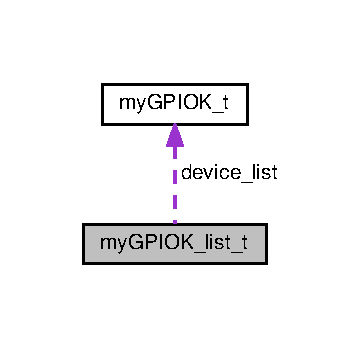
\includegraphics[width=174pt]{structmy_g_p_i_o_k__list__t__coll__graph}
\end{center}
\end{figure}
\subsection*{Campi}
\begin{DoxyCompactItemize}
\item 
\hyperlink{structmy_g_p_i_o_k__t}{my\+G\+P\+I\+O\+K\+\_\+t} $\ast$$\ast$ \hyperlink{structmy_g_p_i_o_k__list__t_a99b54fb4cab6e0b7ea3bd94415bbcca0}{device\+\_\+list}
\item 
uint32\+\_\+t \hyperlink{structmy_g_p_i_o_k__list__t_aeff61809685e5df1b38aec1d871a49bb}{list\+\_\+size}
\item 
uint32\+\_\+t \hyperlink{structmy_g_p_i_o_k__list__t_a170d1d78f27f6ab4c8badaaa4b3f2305}{device\+\_\+count}
\end{DoxyCompactItemize}


\subsection{Descrizione dettagliata}
Struttura dati per la gestione degli oggetti \hyperlink{structmy_g_p_i_o_k__t}{my\+G\+P\+I\+O\+K\+\_\+t} gestiti dal driver. 

La struttura dati, sebbene non strettamente necessaria alla gestione dei diversi oggetti \hyperlink{structmy_g_p_i_o_k__t}{my\+G\+P\+I\+O\+K\+\_\+t}, ciascuno dei quali corrispondente ad un diverso device gestito dal driver my\+G\+P\+I\+OK, è pensata per semplificare l\textquotesingle{}accesso a questi ultimi, tenendo un riferimento a tutti gli oggetti e le strutture dati coinvolte nel funzionamento del modulo in un unico \char`\"{}posto\char`\"{}, accessibile attraverso questa struttura dati. 

\subsection{Documentazione dei campi}
\mbox{\Hypertarget{structmy_g_p_i_o_k__list__t_a170d1d78f27f6ab4c8badaaa4b3f2305}\label{structmy_g_p_i_o_k__list__t_a170d1d78f27f6ab4c8badaaa4b3f2305}} 
\index{my\+G\+P\+I\+O\+K\+\_\+list\+\_\+t@{my\+G\+P\+I\+O\+K\+\_\+list\+\_\+t}!device\+\_\+count@{device\+\_\+count}}
\index{device\+\_\+count@{device\+\_\+count}!my\+G\+P\+I\+O\+K\+\_\+list\+\_\+t@{my\+G\+P\+I\+O\+K\+\_\+list\+\_\+t}}
\subsubsection{\texorpdfstring{device\+\_\+count}{device\_count}}
{\footnotesize\ttfamily uint32\+\_\+t device\+\_\+count}

numero di device correntemente attivi e gestiti dal driver \mbox{\Hypertarget{structmy_g_p_i_o_k__list__t_a99b54fb4cab6e0b7ea3bd94415bbcca0}\label{structmy_g_p_i_o_k__list__t_a99b54fb4cab6e0b7ea3bd94415bbcca0}} 
\index{my\+G\+P\+I\+O\+K\+\_\+list\+\_\+t@{my\+G\+P\+I\+O\+K\+\_\+list\+\_\+t}!device\+\_\+list@{device\+\_\+list}}
\index{device\+\_\+list@{device\+\_\+list}!my\+G\+P\+I\+O\+K\+\_\+list\+\_\+t@{my\+G\+P\+I\+O\+K\+\_\+list\+\_\+t}}
\subsubsection{\texorpdfstring{device\+\_\+list}{device\_list}}
{\footnotesize\ttfamily \hyperlink{structmy_g_p_i_o_k__t}{my\+G\+P\+I\+O\+K\+\_\+t}$\ast$$\ast$ device\+\_\+list}

array di puntatori a struttura \hyperlink{structmy_g_p_i_o_k__t}{my\+G\+P\+I\+O\+K\+\_\+t}, ciascuno dei quali si riferisce ad un device differente \mbox{\Hypertarget{structmy_g_p_i_o_k__list__t_aeff61809685e5df1b38aec1d871a49bb}\label{structmy_g_p_i_o_k__list__t_aeff61809685e5df1b38aec1d871a49bb}} 
\index{my\+G\+P\+I\+O\+K\+\_\+list\+\_\+t@{my\+G\+P\+I\+O\+K\+\_\+list\+\_\+t}!list\+\_\+size@{list\+\_\+size}}
\index{list\+\_\+size@{list\+\_\+size}!my\+G\+P\+I\+O\+K\+\_\+list\+\_\+t@{my\+G\+P\+I\+O\+K\+\_\+list\+\_\+t}}
\subsubsection{\texorpdfstring{list\+\_\+size}{list\_size}}
{\footnotesize\ttfamily uint32\+\_\+t list\+\_\+size}

dimensione dell\textquotesingle{}array, corrisponde al numero massimo di device gestibili, definito in fase di inizializzazione 

La documentazione per questa struct è stata generata a partire dal seguente file\+:\begin{DoxyCompactItemize}
\item 
Src/my\+G\+P\+I\+O/linux-\/driver/\hyperlink{my_g_p_i_o_k__list_8h}{my\+G\+P\+I\+O\+K\+\_\+list.\+h}\end{DoxyCompactItemize}

\hypertarget{structmy_g_p_i_o_k__t}{\section{Riferimenti per la struct my\+G\+P\+I\+O\+K\+\_\+t}
\label{structmy_g_p_i_o_k__t}\index{my\+G\+P\+I\+O\+K\+\_\+t@{my\+G\+P\+I\+O\+K\+\_\+t}}
}


Stuttura per l'astrazione di un device.  


\subsection*{Campi}
\begin{DoxyCompactItemize}
\item 
struct cdev \hyperlink{structmy_g_p_i_o_k__t_acba682fe45d5a1501790dbdb1d99bd6a}{cdev}
\item 
uint32\+\_\+t \hyperlink{structmy_g_p_i_o_k__t_a42a1593ebe61611c4e29413903a373a5}{irq\+Number}
\item 
struct resource \hyperlink{structmy_g_p_i_o_k__t_a565a1848c3ae8026257a74cf169c6941}{rsrc}
\item 
struct resource $\ast$ \hyperlink{structmy_g_p_i_o_k__t_a18c4eb95350c67ccb239a8a39c43c09a}{mreg}
\item 
uint32\+\_\+t \hyperlink{structmy_g_p_i_o_k__t_a0f87b53dc5049a349ef01aa586c0b5dc}{rsrc\+\_\+size}
\item 
void $\ast$ \hyperlink{structmy_g_p_i_o_k__t_af5aef493b3c2bc9d1f036ce0acea9bba}{vrtl\+\_\+addr}
\item 
wait\+\_\+queue\+\_\+head\+\_\+t \hyperlink{structmy_g_p_i_o_k__t_a251570f8e6976ad87411093e330e7b4f}{read\+\_\+queue}
\item 
wait\+\_\+queue\+\_\+head\+\_\+t \hyperlink{structmy_g_p_i_o_k__t_a2080617f88cafd765430573afe7701d1}{poll\+\_\+queue}
\item 
uint32\+\_\+t \hyperlink{structmy_g_p_i_o_k__t_a6fd94ecf2bef1aa7bd105577b660a112}{int\+\_\+occurred}
\item 
spinlock\+\_\+t \hyperlink{structmy_g_p_i_o_k__t_a1e1ddf972b4dc84dd331a0c72e5d9895}{slock\+\_\+int}
\item 
uint32\+\_\+t \hyperlink{structmy_g_p_i_o_k__t_a2da711ac290a9613b8d8af97f122b997}{total\+\_\+irq}
\item 
spinlock\+\_\+t \hyperlink{structmy_g_p_i_o_k__t_ac41bbc7fe03ef25b7f468275fb565d78}{sl\+\_\+total\+\_\+irq}
\end{DoxyCompactItemize}


\subsection{Descrizione dettagliata}
Stuttura per l'astrazione di un device. 

E' buona abitudine, se non quasi indispensabile, definire una struttura dati nella quale contenere tutto cio' che e' legato al device o al driver. In questo modulo viene usata la struttura \hyperlink{structmy_g_p_i_o_k__t}{my\+G\+P\+I\+O\+K\+\_\+t} per contenere tutto cio' che e' necessario al funzionamento del driver. 

\subsection{Documentazione dei campi}
\hypertarget{structmy_g_p_i_o_k__t_acba682fe45d5a1501790dbdb1d99bd6a}{\index{my\+G\+P\+I\+O\+K\+\_\+t@{my\+G\+P\+I\+O\+K\+\_\+t}!cdev@{cdev}}
\index{cdev@{cdev}!my\+G\+P\+I\+O\+K\+\_\+t@{my\+G\+P\+I\+O\+K\+\_\+t}}
\subsubsection[{cdev}]{\setlength{\rightskip}{0pt plus 5cm}struct cdev cdev}}\label{structmy_g_p_i_o_k__t_acba682fe45d5a1501790dbdb1d99bd6a}
Stuttura per l'astrazione di un device a caratteri, Il kernel usa, internamente, una struttura cdev per rappresentare i device a caratteri. Prima che il kernel invochi le funzioni definite dal driver per il device, bisogna allocare e registrare uno, o piu', oggetti cdev. In questo caso e' sufficiente allocare uno solo di questi oggetti. \hypertarget{structmy_g_p_i_o_k__t_a6fd94ecf2bef1aa7bd105577b660a112}{\index{my\+G\+P\+I\+O\+K\+\_\+t@{my\+G\+P\+I\+O\+K\+\_\+t}!int\+\_\+occurred@{int\+\_\+occurred}}
\index{int\+\_\+occurred@{int\+\_\+occurred}!my\+G\+P\+I\+O\+K\+\_\+t@{my\+G\+P\+I\+O\+K\+\_\+t}}
\subsubsection[{int\+\_\+occurred}]{\setlength{\rightskip}{0pt plus 5cm}uint32\+\_\+t int\+\_\+occurred}}\label{structmy_g_p_i_o_k__t_a6fd94ecf2bef1aa7bd105577b660a112}
Flag \char`\"{}interrupt occurred\char`\"{} Il valore viene settato dalla funzione \hyperlink{group___kernel-_module_ga2fc230a12a97aa63e43b2dc4aec73511}{my\+G\+P\+I\+O\+K\+\_\+irq\+\_\+handler()} al manifestarsi di un interrupt, prima di risvegliare i processi in attesa che tale variabile assuma uno specifico valore. I valori con cui questo flag puo' essere settato sono due\+:
\begin{DoxyItemize}
\item M\+Y\+G\+P\+I\+O\+K\+\_\+\+S\+R\+E\+A\+D \+: per la read bloccante.
\item M\+Y\+G\+P\+I\+O\+K\+\_\+\+A\+R\+E\+A\+D \+: pre la read non bloccante.
\end{DoxyItemize}

I processi che effettuano read() bloccante restano bloccati finoche' int\+\_\+occurred \& M\+Y\+G\+P\+I\+O\+\_\+\+S\+R\+E\+A\+D != 0 \hypertarget{structmy_g_p_i_o_k__t_a42a1593ebe61611c4e29413903a373a5}{\index{my\+G\+P\+I\+O\+K\+\_\+t@{my\+G\+P\+I\+O\+K\+\_\+t}!irq\+Number@{irq\+Number}}
\index{irq\+Number@{irq\+Number}!my\+G\+P\+I\+O\+K\+\_\+t@{my\+G\+P\+I\+O\+K\+\_\+t}}
\subsubsection[{irq\+Number}]{\setlength{\rightskip}{0pt plus 5cm}uint32\+\_\+t irq\+Number}}\label{structmy_g_p_i_o_k__t_a42a1593ebe61611c4e29413903a373a5}
interrupt-\/number a cui il device e' connesso. Restituito dalla chiamata alla funzione irq\+\_\+of\+\_\+parse\+\_\+and\+\_\+map() \hypertarget{structmy_g_p_i_o_k__t_a18c4eb95350c67ccb239a8a39c43c09a}{\index{my\+G\+P\+I\+O\+K\+\_\+t@{my\+G\+P\+I\+O\+K\+\_\+t}!mreg@{mreg}}
\index{mreg@{mreg}!my\+G\+P\+I\+O\+K\+\_\+t@{my\+G\+P\+I\+O\+K\+\_\+t}}
\subsubsection[{mreg}]{\setlength{\rightskip}{0pt plus 5cm}struct resource$\ast$ mreg}}\label{structmy_g_p_i_o_k__t_a18c4eb95350c67ccb239a8a39c43c09a}
puntatre alla regione di memoria cui il device e' mapapto \hypertarget{structmy_g_p_i_o_k__t_a2080617f88cafd765430573afe7701d1}{\index{my\+G\+P\+I\+O\+K\+\_\+t@{my\+G\+P\+I\+O\+K\+\_\+t}!poll\+\_\+queue@{poll\+\_\+queue}}
\index{poll\+\_\+queue@{poll\+\_\+queue}!my\+G\+P\+I\+O\+K\+\_\+t@{my\+G\+P\+I\+O\+K\+\_\+t}}
\subsubsection[{poll\+\_\+queue}]{\setlength{\rightskip}{0pt plus 5cm}wait\+\_\+queue\+\_\+head\+\_\+t poll\+\_\+queue}}\label{structmy_g_p_i_o_k__t_a2080617f88cafd765430573afe7701d1}
wait queue per la system-\/call poll() \hypertarget{structmy_g_p_i_o_k__t_a251570f8e6976ad87411093e330e7b4f}{\index{my\+G\+P\+I\+O\+K\+\_\+t@{my\+G\+P\+I\+O\+K\+\_\+t}!read\+\_\+queue@{read\+\_\+queue}}
\index{read\+\_\+queue@{read\+\_\+queue}!my\+G\+P\+I\+O\+K\+\_\+t@{my\+G\+P\+I\+O\+K\+\_\+t}}
\subsubsection[{read\+\_\+queue}]{\setlength{\rightskip}{0pt plus 5cm}wait\+\_\+queue\+\_\+head\+\_\+t read\+\_\+queue}}\label{structmy_g_p_i_o_k__t_a251570f8e6976ad87411093e330e7b4f}
wait queue per la system-\/call read() Una chiamata a read() potrebbe arrivare quando i dati non sono disponibili, ma potrebbero esserlo in futuro, oppure, una chiamata a write() potrebbe avvenire quando il device non e' in grado di accettare altri dati (perche' il suo buffer di ingresso potrebbe essere pieno). Il processo chiamante non ha la minima conoscenza delle dinamiche interne del device, per cui, nell'impossibilita' di servire la richiesta, il driver deve bloccare il processo e metterlo tra i processi \char`\"{}sleeping\char`\"{}, fin quando la richiesta non puo' essere servita. Tutti i processi in attesa di un particolare evento vengono posti all'interno della stessa wait queue. In linux una wait queue viene implementata da una struttura dati wait\+\_\+queue\+\_\+head\+\_\+t, definita in $<$linux/wait.\+h$>$. \hypertarget{structmy_g_p_i_o_k__t_a565a1848c3ae8026257a74cf169c6941}{\index{my\+G\+P\+I\+O\+K\+\_\+t@{my\+G\+P\+I\+O\+K\+\_\+t}!rsrc@{rsrc}}
\index{rsrc@{rsrc}!my\+G\+P\+I\+O\+K\+\_\+t@{my\+G\+P\+I\+O\+K\+\_\+t}}
\subsubsection[{rsrc}]{\setlength{\rightskip}{0pt plus 5cm}struct resource rsrc}}\label{structmy_g_p_i_o_k__t_a565a1848c3ae8026257a74cf169c6941}
Struttura che astrae una risorsa device, dal punto di vista della memoria alla quale la risorsa e' mappata. In particolare i campi \char`\"{}start\char`\"{} ed \char`\"{}end\char`\"{} contengono, rispettivamente, il primo e l'ultimo indirizzo fisico a cui il device e' mappato. \hypertarget{structmy_g_p_i_o_k__t_a0f87b53dc5049a349ef01aa586c0b5dc}{\index{my\+G\+P\+I\+O\+K\+\_\+t@{my\+G\+P\+I\+O\+K\+\_\+t}!rsrc\+\_\+size@{rsrc\+\_\+size}}
\index{rsrc\+\_\+size@{rsrc\+\_\+size}!my\+G\+P\+I\+O\+K\+\_\+t@{my\+G\+P\+I\+O\+K\+\_\+t}}
\subsubsection[{rsrc\+\_\+size}]{\setlength{\rightskip}{0pt plus 5cm}uint32\+\_\+t rsrc\+\_\+size}}\label{structmy_g_p_i_o_k__t_a0f87b53dc5049a349ef01aa586c0b5dc}
rsrc.\+end -\/ rsrc.\+start numero di indirizzi associati alla periferica. occorre per effettuare il mapping indirizzo fisico -\/ indirizzo virtuale \hypertarget{structmy_g_p_i_o_k__t_ac41bbc7fe03ef25b7f468275fb565d78}{\index{my\+G\+P\+I\+O\+K\+\_\+t@{my\+G\+P\+I\+O\+K\+\_\+t}!sl\+\_\+total\+\_\+irq@{sl\+\_\+total\+\_\+irq}}
\index{sl\+\_\+total\+\_\+irq@{sl\+\_\+total\+\_\+irq}!my\+G\+P\+I\+O\+K\+\_\+t@{my\+G\+P\+I\+O\+K\+\_\+t}}
\subsubsection[{sl\+\_\+total\+\_\+irq}]{\setlength{\rightskip}{0pt plus 5cm}spinlock\+\_\+t sl\+\_\+total\+\_\+irq}}\label{structmy_g_p_i_o_k__t_ac41bbc7fe03ef25b7f468275fb565d78}
Spinlock usato per garantire l'accesso in mutua esclusione alla variabile total\+\_\+irq da parte delle funzioni del modulo \hypertarget{structmy_g_p_i_o_k__t_a1e1ddf972b4dc84dd331a0c72e5d9895}{\index{my\+G\+P\+I\+O\+K\+\_\+t@{my\+G\+P\+I\+O\+K\+\_\+t}!slock\+\_\+int@{slock\+\_\+int}}
\index{slock\+\_\+int@{slock\+\_\+int}!my\+G\+P\+I\+O\+K\+\_\+t@{my\+G\+P\+I\+O\+K\+\_\+t}}
\subsubsection[{slock\+\_\+int}]{\setlength{\rightskip}{0pt plus 5cm}spinlock\+\_\+t slock\+\_\+int}}\label{structmy_g_p_i_o_k__t_a1e1ddf972b4dc84dd331a0c72e5d9895}
Spinlock usato per garantire l'accesso in mutua esclusione alla variabile int\+\_\+occurred da parte delle funzioni del modulo. I semafori sono uno strumento potentissimo per per l'implementazione di sezioni critiche, ma non possono essere usati in codice non interrompibile. Gli spilock sono come i semafori, ma possono essere usati anche in codice non interrompibile, come puo' esserlo un modulo kernel. Sostanzialmente se uno spinlock e' gia' stato acquisito da qualcun altro, si entra in un hot-\/loop dal quale si esce solo quando chi possiede lo spinlock lo rilascia. Trattandosi di moduli kernel, e' di vitale importanza che la sezione critica sia quanto piu' piccola possibile. Ovviamente l'implementazione e' \char`\"{}un
po'\char`\"{} piu' complessa di come e' stata descritta, ma il concetto e' questo. Gli spinlock sono definiti in $<$linux/spinlock.\+h$>$. \hypertarget{structmy_g_p_i_o_k__t_a2da711ac290a9613b8d8af97f122b997}{\index{my\+G\+P\+I\+O\+K\+\_\+t@{my\+G\+P\+I\+O\+K\+\_\+t}!total\+\_\+irq@{total\+\_\+irq}}
\index{total\+\_\+irq@{total\+\_\+irq}!my\+G\+P\+I\+O\+K\+\_\+t@{my\+G\+P\+I\+O\+K\+\_\+t}}
\subsubsection[{total\+\_\+irq}]{\setlength{\rightskip}{0pt plus 5cm}uint32\+\_\+t total\+\_\+irq}}\label{structmy_g_p_i_o_k__t_a2da711ac290a9613b8d8af97f122b997}
numero totale di interrupt manifestatesi \hypertarget{structmy_g_p_i_o_k__t_af5aef493b3c2bc9d1f036ce0acea9bba}{\index{my\+G\+P\+I\+O\+K\+\_\+t@{my\+G\+P\+I\+O\+K\+\_\+t}!vrtl\+\_\+addr@{vrtl\+\_\+addr}}
\index{vrtl\+\_\+addr@{vrtl\+\_\+addr}!my\+G\+P\+I\+O\+K\+\_\+t@{my\+G\+P\+I\+O\+K\+\_\+t}}
\subsubsection[{vrtl\+\_\+addr}]{\setlength{\rightskip}{0pt plus 5cm}void$\ast$ vrtl\+\_\+addr}}\label{structmy_g_p_i_o_k__t_af5aef493b3c2bc9d1f036ce0acea9bba}
indirizzo virtuale della periferica 

La documentazione per questa struct è stata generata a partire dal seguente file\+:\begin{DoxyCompactItemize}
\item 
my\+G\+P\+I\+O/linux-\/driver/kernel\+\_\+module/kernel\+\_\+module/\hyperlink{my_g_p_i_o_k_8c}{my\+G\+P\+I\+O\+K.\+c}\end{DoxyCompactItemize}

\hypertarget{structparam__t}{\section{Riferimenti per la struct param\+\_\+t}
\label{structparam__t}\index{param\+\_\+t@{param\+\_\+t}}
}
\subsection*{Campi}
\begin{DoxyCompactItemize}
\item 
int \hyperlink{structparam__t_a52701f5f8091598d5c5ac1bb80cd2070}{dev\+\_\+descr}
\item 
uint8\+\_\+t \hyperlink{structparam__t_aec948fb30e99b1eda7e3d9ff741d417a}{op\+\_\+mode}
\item 
uint32\+\_\+t \hyperlink{structparam__t_a007b34e09ccda08824bc74ab9d86c5a8}{mode\+\_\+value}
\item 
uint8\+\_\+t \hyperlink{structparam__t_a67752de733f167918a4e966354183a69}{op\+\_\+write}
\item 
uint32\+\_\+t \hyperlink{structparam__t_a09e0cff25312ab7f748a3063c038a2d9}{write\+\_\+value}
\item 
uint8\+\_\+t \hyperlink{structparam__t_ae66d5c3154a115636a63227b7489a6eb}{op\+\_\+read}
\end{DoxyCompactItemize}


\subsection{Documentazione dei campi}
\hypertarget{structparam__t_a52701f5f8091598d5c5ac1bb80cd2070}{\index{param\+\_\+t@{param\+\_\+t}!dev\+\_\+descr@{dev\+\_\+descr}}
\index{dev\+\_\+descr@{dev\+\_\+descr}!param\+\_\+t@{param\+\_\+t}}
\subsubsection[{dev\+\_\+descr}]{\setlength{\rightskip}{0pt plus 5cm}int dev\+\_\+descr}}\label{structparam__t_a52701f5f8091598d5c5ac1bb80cd2070}
\hypertarget{structparam__t_a007b34e09ccda08824bc74ab9d86c5a8}{\index{param\+\_\+t@{param\+\_\+t}!mode\+\_\+value@{mode\+\_\+value}}
\index{mode\+\_\+value@{mode\+\_\+value}!param\+\_\+t@{param\+\_\+t}}
\subsubsection[{mode\+\_\+value}]{\setlength{\rightskip}{0pt plus 5cm}uint32\+\_\+t mode\+\_\+value}}\label{structparam__t_a007b34e09ccda08824bc74ab9d86c5a8}
\hypertarget{structparam__t_aec948fb30e99b1eda7e3d9ff741d417a}{\index{param\+\_\+t@{param\+\_\+t}!op\+\_\+mode@{op\+\_\+mode}}
\index{op\+\_\+mode@{op\+\_\+mode}!param\+\_\+t@{param\+\_\+t}}
\subsubsection[{op\+\_\+mode}]{\setlength{\rightskip}{0pt plus 5cm}uint8\+\_\+t op\+\_\+mode}}\label{structparam__t_aec948fb30e99b1eda7e3d9ff741d417a}
\hypertarget{structparam__t_ae66d5c3154a115636a63227b7489a6eb}{\index{param\+\_\+t@{param\+\_\+t}!op\+\_\+read@{op\+\_\+read}}
\index{op\+\_\+read@{op\+\_\+read}!param\+\_\+t@{param\+\_\+t}}
\subsubsection[{op\+\_\+read}]{\setlength{\rightskip}{0pt plus 5cm}uint8\+\_\+t op\+\_\+read}}\label{structparam__t_ae66d5c3154a115636a63227b7489a6eb}
\hypertarget{structparam__t_a67752de733f167918a4e966354183a69}{\index{param\+\_\+t@{param\+\_\+t}!op\+\_\+write@{op\+\_\+write}}
\index{op\+\_\+write@{op\+\_\+write}!param\+\_\+t@{param\+\_\+t}}
\subsubsection[{op\+\_\+write}]{\setlength{\rightskip}{0pt plus 5cm}uint8\+\_\+t op\+\_\+write}}\label{structparam__t_a67752de733f167918a4e966354183a69}
\hypertarget{structparam__t_a09e0cff25312ab7f748a3063c038a2d9}{\index{param\+\_\+t@{param\+\_\+t}!write\+\_\+value@{write\+\_\+value}}
\index{write\+\_\+value@{write\+\_\+value}!param\+\_\+t@{param\+\_\+t}}
\subsubsection[{write\+\_\+value}]{\setlength{\rightskip}{0pt plus 5cm}uint32\+\_\+t write\+\_\+value}}\label{structparam__t_a09e0cff25312ab7f748a3063c038a2d9}


La documentazione per questa struct è stata generata a partire dal seguente file\+:\begin{DoxyCompactItemize}
\item 
my\+G\+P\+I\+O/linux-\/driver/kernel\+\_\+module/userspace\+\_\+program/\hyperlink{gpio_8c}{gpio.\+c}\end{DoxyCompactItemize}

\hypertarget{struct_zybo_button__t}{\section{Riferimenti per la struct Zybo\+Button\+\_\+t}
\label{struct_zybo_button__t}\index{Zybo\+Button\+\_\+t@{Zybo\+Button\+\_\+t}}
}


Struttura opaca che astrae l'insieme dei button presenti sulla board Digilent Zybo;.  




{\ttfamily \#include $<$Zybo\+Button.\+h$>$}



Diagramma di collaborazione per Zybo\+Button\+\_\+t\+:\nopagebreak
\begin{figure}[H]
\begin{center}
\leavevmode
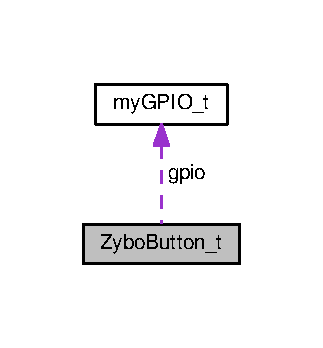
\includegraphics[width=155pt]{struct_zybo_button__t__coll__graph}
\end{center}
\end{figure}
\subsection*{Campi}
\begin{DoxyCompactItemize}
\item 
\hyperlink{structmy_g_p_i_o__t}{my\+G\+P\+I\+O\+\_\+t} $\ast$ \hyperlink{struct_zybo_button__t_ac37ddc7c58d246d233dfb38037020184}{gpio}
\item 
\hyperlink{group__bare-metal_ga402a0d20afc0cb7c25554b8b023f4253}{my\+G\+P\+I\+O\+\_\+mask} \hyperlink{struct_zybo_button__t_ad462a15a55883fd4c86d2be9e11968a7}{Button3\+\_\+pin}
\item 
\hyperlink{group__bare-metal_ga402a0d20afc0cb7c25554b8b023f4253}{my\+G\+P\+I\+O\+\_\+mask} \hyperlink{struct_zybo_button__t_a3b4fe634c2d98ce55fdef526c2d230d1}{Button2\+\_\+pin}
\item 
\hyperlink{group__bare-metal_ga402a0d20afc0cb7c25554b8b023f4253}{my\+G\+P\+I\+O\+\_\+mask} \hyperlink{struct_zybo_button__t_a6cb60bb285e32e29c51c15e85206aaeb}{Button1\+\_\+pin}
\item 
\hyperlink{group__bare-metal_ga402a0d20afc0cb7c25554b8b023f4253}{my\+G\+P\+I\+O\+\_\+mask} \hyperlink{struct_zybo_button__t_af7d7d5a9c9fc174e8f4ee4c762c2abee}{Button0\+\_\+pin}
\end{DoxyCompactItemize}


\subsection{Descrizione dettagliata}
Struttura opaca che astrae l'insieme dei button presenti sulla board Digilent Zybo;. \begin{Desc}
\item[Esempi\+: ]\par
\hyperlink{bsp_example_8c-example}{bsp\+\_\+example.\+c}.\end{Desc}


\subsection{Documentazione dei campi}
\hypertarget{struct_zybo_button__t_af7d7d5a9c9fc174e8f4ee4c762c2abee}{\index{Zybo\+Button\+\_\+t@{Zybo\+Button\+\_\+t}!Button0\+\_\+pin@{Button0\+\_\+pin}}
\index{Button0\+\_\+pin@{Button0\+\_\+pin}!Zybo\+Button\+\_\+t@{Zybo\+Button\+\_\+t}}
\subsubsection[{Button0\+\_\+pin}]{\setlength{\rightskip}{0pt plus 5cm}{\bf my\+G\+P\+I\+O\+\_\+mask} Button0\+\_\+pin}}\label{struct_zybo_button__t_af7d7d5a9c9fc174e8f4ee4c762c2abee}
maschera di selezione per il particolare bit del device my\+G\+P\+I\+O connesso al button numero 0 della board Zybo \hypertarget{struct_zybo_button__t_a6cb60bb285e32e29c51c15e85206aaeb}{\index{Zybo\+Button\+\_\+t@{Zybo\+Button\+\_\+t}!Button1\+\_\+pin@{Button1\+\_\+pin}}
\index{Button1\+\_\+pin@{Button1\+\_\+pin}!Zybo\+Button\+\_\+t@{Zybo\+Button\+\_\+t}}
\subsubsection[{Button1\+\_\+pin}]{\setlength{\rightskip}{0pt plus 5cm}{\bf my\+G\+P\+I\+O\+\_\+mask} Button1\+\_\+pin}}\label{struct_zybo_button__t_a6cb60bb285e32e29c51c15e85206aaeb}
maschera di selezione per il particolare bit del device my\+G\+P\+I\+O connesso al button numero 1 della board Zybo \hypertarget{struct_zybo_button__t_a3b4fe634c2d98ce55fdef526c2d230d1}{\index{Zybo\+Button\+\_\+t@{Zybo\+Button\+\_\+t}!Button2\+\_\+pin@{Button2\+\_\+pin}}
\index{Button2\+\_\+pin@{Button2\+\_\+pin}!Zybo\+Button\+\_\+t@{Zybo\+Button\+\_\+t}}
\subsubsection[{Button2\+\_\+pin}]{\setlength{\rightskip}{0pt plus 5cm}{\bf my\+G\+P\+I\+O\+\_\+mask} Button2\+\_\+pin}}\label{struct_zybo_button__t_a3b4fe634c2d98ce55fdef526c2d230d1}
maschera di selezione per il particolare bit del device my\+G\+P\+I\+O connesso al button numero 2 della board Zybo \hypertarget{struct_zybo_button__t_ad462a15a55883fd4c86d2be9e11968a7}{\index{Zybo\+Button\+\_\+t@{Zybo\+Button\+\_\+t}!Button3\+\_\+pin@{Button3\+\_\+pin}}
\index{Button3\+\_\+pin@{Button3\+\_\+pin}!Zybo\+Button\+\_\+t@{Zybo\+Button\+\_\+t}}
\subsubsection[{Button3\+\_\+pin}]{\setlength{\rightskip}{0pt plus 5cm}{\bf my\+G\+P\+I\+O\+\_\+mask} Button3\+\_\+pin}}\label{struct_zybo_button__t_ad462a15a55883fd4c86d2be9e11968a7}
maschera di selezione per il particolare bit del device my\+G\+P\+I\+O connesso al button numero 3 della board Zybo \hypertarget{struct_zybo_button__t_ac37ddc7c58d246d233dfb38037020184}{\index{Zybo\+Button\+\_\+t@{Zybo\+Button\+\_\+t}!gpio@{gpio}}
\index{gpio@{gpio}!Zybo\+Button\+\_\+t@{Zybo\+Button\+\_\+t}}
\subsubsection[{gpio}]{\setlength{\rightskip}{0pt plus 5cm}{\bf my\+G\+P\+I\+O\+\_\+t}$\ast$ gpio}}\label{struct_zybo_button__t_ac37ddc7c58d246d233dfb38037020184}
puntatore a struttura \hyperlink{structmy_g_p_i_o__t}{my\+G\+P\+I\+O\+\_\+t}, che astrae il particolare my\+G\+P\+I\+O usato per la lettura dello stato dei button presenti sulla board 

La documentazione per questa struct è stata generata a partire dal seguente file\+:\begin{DoxyCompactItemize}
\item 
Src/my\+G\+P\+I\+O/bare-\/metal/\+Zybo\+B\+S\+P/\hyperlink{_zybo_button_8h}{Zybo\+Button.\+h}\end{DoxyCompactItemize}

\hypertarget{struct_zybo_led__t}{\section{Riferimenti per la struct Zybo\+Led\+\_\+t}
\label{struct_zybo_led__t}\index{Zybo\+Led\+\_\+t@{Zybo\+Led\+\_\+t}}
}


Struttura opaca che astrae l'insieme dei Led presenti sulla board Digilent Zybo;.  




{\ttfamily \#include $<$Zybo\+Led.\+h$>$}



Diagramma di collaborazione per Zybo\+Led\+\_\+t\+:
\nopagebreak
\begin{figure}[H]
\begin{center}
\leavevmode
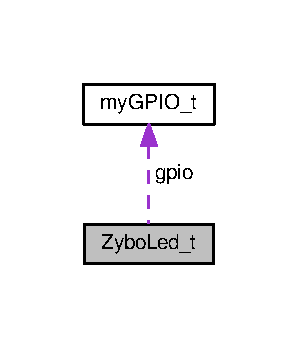
\includegraphics[width=143pt]{struct_zybo_led__t__coll__graph}
\end{center}
\end{figure}
\subsection*{Campi}
\begin{DoxyCompactItemize}
\item 
\hyperlink{structmy_g_p_i_o__t}{my\+G\+P\+I\+O\+\_\+t} $\ast$ \hyperlink{struct_zybo_led__t_ac37ddc7c58d246d233dfb38037020184}{gpio}
\item 
\hyperlink{group__my_g_p_i_o_ga402a0d20afc0cb7c25554b8b023f4253}{my\+G\+P\+I\+O\+\_\+mask} \hyperlink{struct_zybo_led__t_afc64d1407f30615e374bf9f06721842a}{Led3\+\_\+pin}
\item 
\hyperlink{group__my_g_p_i_o_ga402a0d20afc0cb7c25554b8b023f4253}{my\+G\+P\+I\+O\+\_\+mask} \hyperlink{struct_zybo_led__t_a4213c78e5a02b1476222e989c2eceb04}{Led2\+\_\+pin}
\item 
\hyperlink{group__my_g_p_i_o_ga402a0d20afc0cb7c25554b8b023f4253}{my\+G\+P\+I\+O\+\_\+mask} \hyperlink{struct_zybo_led__t_adc78fb167f1dd6693910813d4ec5930e}{Led1\+\_\+pin}
\item 
\hyperlink{group__my_g_p_i_o_ga402a0d20afc0cb7c25554b8b023f4253}{my\+G\+P\+I\+O\+\_\+mask} \hyperlink{struct_zybo_led__t_ac5afef2eef91d5533a23435cfcc60104}{Led0\+\_\+pin}
\end{DoxyCompactItemize}


\subsection{Descrizione dettagliata}
Struttura opaca che astrae l'insieme dei Led presenti sulla board Digilent Zybo;. 

\subsection{Documentazione dei campi}
\hypertarget{struct_zybo_led__t_ac37ddc7c58d246d233dfb38037020184}{\index{Zybo\+Led\+\_\+t@{Zybo\+Led\+\_\+t}!gpio@{gpio}}
\index{gpio@{gpio}!Zybo\+Led\+\_\+t@{Zybo\+Led\+\_\+t}}
\subsubsection[{gpio}]{\setlength{\rightskip}{0pt plus 5cm}{\bf my\+G\+P\+I\+O\+\_\+t}$\ast$ gpio}}\label{struct_zybo_led__t_ac37ddc7c58d246d233dfb38037020184}
puntatore a struttura \hyperlink{structmy_g_p_i_o__t}{my\+G\+P\+I\+O\+\_\+t}, che astrae il particolare G\+P\+I\+O usato per il pilotaggio dei led presenti sulla board \hypertarget{struct_zybo_led__t_ac5afef2eef91d5533a23435cfcc60104}{\index{Zybo\+Led\+\_\+t@{Zybo\+Led\+\_\+t}!Led0\+\_\+pin@{Led0\+\_\+pin}}
\index{Led0\+\_\+pin@{Led0\+\_\+pin}!Zybo\+Led\+\_\+t@{Zybo\+Led\+\_\+t}}
\subsubsection[{Led0\+\_\+pin}]{\setlength{\rightskip}{0pt plus 5cm}{\bf my\+G\+P\+I\+O\+\_\+mask} Led0\+\_\+pin}}\label{struct_zybo_led__t_ac5afef2eef91d5533a23435cfcc60104}
maschera di selezione per il particolare bit del device G\+P\+I\+O usato per il pilotaggio del led numero 0 della board Zybo \hypertarget{struct_zybo_led__t_adc78fb167f1dd6693910813d4ec5930e}{\index{Zybo\+Led\+\_\+t@{Zybo\+Led\+\_\+t}!Led1\+\_\+pin@{Led1\+\_\+pin}}
\index{Led1\+\_\+pin@{Led1\+\_\+pin}!Zybo\+Led\+\_\+t@{Zybo\+Led\+\_\+t}}
\subsubsection[{Led1\+\_\+pin}]{\setlength{\rightskip}{0pt plus 5cm}{\bf my\+G\+P\+I\+O\+\_\+mask} Led1\+\_\+pin}}\label{struct_zybo_led__t_adc78fb167f1dd6693910813d4ec5930e}
maschera di selezione per il particolare bit del device G\+P\+I\+O usato per il pilotaggio del led numero 1 della board Zybo \hypertarget{struct_zybo_led__t_a4213c78e5a02b1476222e989c2eceb04}{\index{Zybo\+Led\+\_\+t@{Zybo\+Led\+\_\+t}!Led2\+\_\+pin@{Led2\+\_\+pin}}
\index{Led2\+\_\+pin@{Led2\+\_\+pin}!Zybo\+Led\+\_\+t@{Zybo\+Led\+\_\+t}}
\subsubsection[{Led2\+\_\+pin}]{\setlength{\rightskip}{0pt plus 5cm}{\bf my\+G\+P\+I\+O\+\_\+mask} Led2\+\_\+pin}}\label{struct_zybo_led__t_a4213c78e5a02b1476222e989c2eceb04}
maschera di selezione per il particolare bit del device G\+P\+I\+O usato per il pilotaggio del led numero 2 della board Zybo \hypertarget{struct_zybo_led__t_afc64d1407f30615e374bf9f06721842a}{\index{Zybo\+Led\+\_\+t@{Zybo\+Led\+\_\+t}!Led3\+\_\+pin@{Led3\+\_\+pin}}
\index{Led3\+\_\+pin@{Led3\+\_\+pin}!Zybo\+Led\+\_\+t@{Zybo\+Led\+\_\+t}}
\subsubsection[{Led3\+\_\+pin}]{\setlength{\rightskip}{0pt plus 5cm}{\bf my\+G\+P\+I\+O\+\_\+mask} Led3\+\_\+pin}}\label{struct_zybo_led__t_afc64d1407f30615e374bf9f06721842a}
maschera di selezione per il particolare bit del device G\+P\+I\+O usato per il pilotaggio del led numero 3 della board Zybo 

La documentazione per questa struct è stata generata a partire dal seguente file\+:\begin{DoxyCompactItemize}
\item 
Zybo/\hyperlink{_zybo_led_8h}{Zybo\+Led.\+h}\end{DoxyCompactItemize}

\hypertarget{struct_zybo_switch__t}{\section{Riferimenti per la struct Zybo\+Switch\+\_\+t}
\label{struct_zybo_switch__t}\index{Zybo\+Switch\+\_\+t@{Zybo\+Switch\+\_\+t}}
}


Struttura opaca che astrae l'insieme degli switch presenti sulla board Digilent Zybo;.  




{\ttfamily \#include $<$Zybo\+Switch.\+h$>$}



Diagramma di collaborazione per Zybo\+Switch\+\_\+t\+:
\nopagebreak
\begin{figure}[H]
\begin{center}
\leavevmode
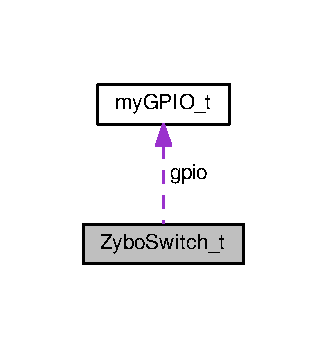
\includegraphics[width=157pt]{struct_zybo_switch__t__coll__graph}
\end{center}
\end{figure}
\subsection*{Campi}
\begin{DoxyCompactItemize}
\item 
\hypertarget{struct_zybo_switch__t_acb3116190992a4d8d26545c103304d27}{\hyperlink{struct_g_p_i_o__t}{G\+P\+I\+O\+\_\+t} $\ast$ {\bfseries gpio}}\label{struct_zybo_switch__t_acb3116190992a4d8d26545c103304d27}

\item 
\hypertarget{struct_zybo_switch__t_a6b95420b88fe8c1fd7f347ce3ae1906b}{G\+P\+I\+O\+\_\+mask {\bfseries Switch3\+\_\+pin}}\label{struct_zybo_switch__t_a6b95420b88fe8c1fd7f347ce3ae1906b}

\item 
\hypertarget{struct_zybo_switch__t_a33eda4a0115ef585edd90078924ca56e}{G\+P\+I\+O\+\_\+mask {\bfseries Switch2\+\_\+pin}}\label{struct_zybo_switch__t_a33eda4a0115ef585edd90078924ca56e}

\item 
\hypertarget{struct_zybo_switch__t_a6a3a5739e7e8f138241cafeeb7c1a33f}{G\+P\+I\+O\+\_\+mask {\bfseries Switch1\+\_\+pin}}\label{struct_zybo_switch__t_a6a3a5739e7e8f138241cafeeb7c1a33f}

\item 
\hypertarget{struct_zybo_switch__t_a5b7f83cd96441b7d1692710c6499147c}{G\+P\+I\+O\+\_\+mask {\bfseries Switch0\+\_\+pin}}\label{struct_zybo_switch__t_a5b7f83cd96441b7d1692710c6499147c}

\end{DoxyCompactItemize}


\subsection{Descrizione dettagliata}
Struttura opaca che astrae l'insieme degli switch presenti sulla board Digilent Zybo;. 

La documentazione per questa struct è stata generata a partire dal seguente file\+:\begin{DoxyCompactItemize}
\item 
Zybo/Zybo\+Switch.\+h\end{DoxyCompactItemize}

\chapter{Documentazione dei file}
\hypertarget{interrupt__bare_8c}{\section{Riferimenti per il file Src/\+Examples/interrupt\+\_\+bare.c}
\label{interrupt__bare_8c}\index{Src/\+Examples/interrupt\+\_\+bare.\+c@{Src/\+Examples/interrupt\+\_\+bare.\+c}}
}
{\ttfamily \#include \char`\"{}xparameters.\+h\char`\"{}}\\*
{\ttfamily \#include \char`\"{}xscugic.\+h\char`\"{}}\\*
{\ttfamily \#include \char`\"{}my\+G\+P\+I\+O.\+h\char`\"{}}\\*
Grafo delle dipendenze di inclusione per interrupt\+\_\+bare.\+c\+:\nopagebreak
\begin{figure}[H]
\begin{center}
\leavevmode
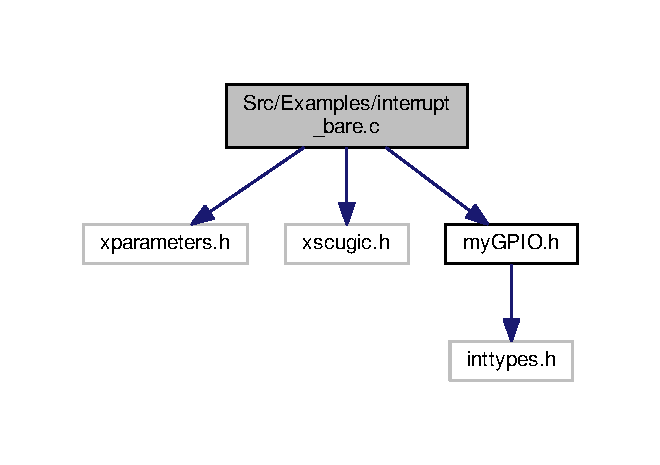
\includegraphics[width=317pt]{interrupt__bare_8c__incl}
\end{center}
\end{figure}
\subsection*{Definizioni}
\begin{DoxyCompactItemize}
\item 
\#define \hyperlink{interrupt__bare_8c_a145e4211eed7013a18d03ed032f0f229}{led\+\_\+base\+\_\+addr}~X\+P\+A\+R\+\_\+\+M\+Y\+G\+P\+I\+O\+\_\+0\+\_\+\+S00\+\_\+\+A\+X\+I\+\_\+\+B\+A\+S\+E\+A\+D\+D\+R
\item 
\#define \hyperlink{interrupt__bare_8c_aedc39629300adb6d9f8b1359eb2f7024}{btn\+\_\+base\+\_\+addr}~X\+P\+A\+R\+\_\+\+M\+Y\+G\+P\+I\+O\+\_\+1\+\_\+\+S00\+\_\+\+A\+X\+I\+\_\+\+B\+A\+S\+E\+A\+D\+D\+R
\item 
\#define \hyperlink{interrupt__bare_8c_a0f79b2ec9c50221371b1a5c027654774}{swc\+\_\+base\+\_\+addr}~X\+P\+A\+R\+\_\+\+M\+Y\+G\+P\+I\+O\+\_\+2\+\_\+\+S00\+\_\+\+A\+X\+I\+\_\+\+B\+A\+S\+E\+A\+D\+D\+R
\item 
\#define \hyperlink{interrupt__bare_8c_a8d6cec3bea27d442869c2a25cb8cd41b}{led\+\_\+irq\+\_\+line}~X\+P\+A\+R\+\_\+\+F\+A\+B\+R\+I\+C\+\_\+\+M\+Y\+G\+P\+I\+O\+\_\+0\+\_\+\+I\+N\+T\+E\+R\+R\+U\+P\+T\+\_\+\+I\+N\+T\+R
\item 
\#define \hyperlink{interrupt__bare_8c_ab5602e3672ec6d03f39d2229dbcb9f74}{btn\+\_\+irq\+\_\+line}~X\+P\+A\+R\+\_\+\+F\+A\+B\+R\+I\+C\+\_\+\+M\+Y\+G\+P\+I\+O\+\_\+1\+\_\+\+I\+N\+T\+E\+R\+R\+U\+P\+T\+\_\+\+I\+N\+T\+R
\item 
\#define \hyperlink{interrupt__bare_8c_a48d05dc71b54a160af13c8e31e9000b1}{swc\+\_\+irq\+\_\+line}~X\+P\+A\+R\+\_\+\+F\+A\+B\+R\+I\+C\+\_\+\+M\+Y\+G\+P\+I\+O\+\_\+2\+\_\+\+I\+N\+T\+E\+R\+R\+U\+P\+T\+\_\+\+I\+N\+T\+R
\item 
\#define \hyperlink{interrupt__bare_8c_a22782ed5aaa2e8d89334d159d14753b5}{gic\+\_\+id}~X\+P\+A\+R\+\_\+\+S\+C\+U\+G\+I\+C\+\_\+0\+\_\+\+D\+E\+V\+I\+C\+E\+\_\+\+I\+D
\end{DoxyCompactItemize}
\subsection*{Funzioni}
\begin{DoxyCompactItemize}
\item 
void \hyperlink{interrupt__bare_8c_afdbe206b3c49f019757ab09b3cf52b9c}{gpio\+\_\+init} (void)
\item 
void \hyperlink{interrupt__bare_8c_aa4eac585cb67311e3e5fd374d6b09ad4}{btn\+\_\+isr} (void $\ast$)
\item 
void \hyperlink{interrupt__bare_8c_ad05dc46b6c6da383d687c5116864b4ed}{swc\+\_\+isr} (void $\ast$)
\item 
int \hyperlink{interrupt__bare_8c_ad4c208e7b28dadf641bc3ec5b290d87d}{int\+\_\+config} (void)
\item 
int \hyperlink{interrupt__bare_8c_ae66f6b31b5ad750f1fe042a706a4e3d4}{main} ()
\end{DoxyCompactItemize}
\subsection*{Variabili}
\begin{DoxyCompactItemize}
\item 
\hyperlink{structmy_g_p_i_o__t}{my\+G\+P\+I\+O\+\_\+t} \hyperlink{interrupt__bare_8c_ac523aaaf082570c199faf2a98e03c219}{led\+\_\+gpio}
\item 
\hyperlink{structmy_g_p_i_o__t}{my\+G\+P\+I\+O\+\_\+t} \hyperlink{interrupt__bare_8c_ac77d5df697b8a0d64704dee5f1433832}{btn\+\_\+gpio}
\item 
\hyperlink{structmy_g_p_i_o__t}{my\+G\+P\+I\+O\+\_\+t} \hyperlink{interrupt__bare_8c_ac2f1233c00752afeb2ecfd305c5fe36a}{swc\+\_\+gpio}
\item 
X\+Scu\+Gic \hyperlink{interrupt__bare_8c_a0ad1175dbe99ac3f36c814258ec4f8c6}{G\+I\+C}
\end{DoxyCompactItemize}


\subsection{Documentazione delle definizioni}
\hypertarget{interrupt__bare_8c_aedc39629300adb6d9f8b1359eb2f7024}{\index{interrupt\+\_\+bare.\+c@{interrupt\+\_\+bare.\+c}!btn\+\_\+base\+\_\+addr@{btn\+\_\+base\+\_\+addr}}
\index{btn\+\_\+base\+\_\+addr@{btn\+\_\+base\+\_\+addr}!interrupt\+\_\+bare.\+c@{interrupt\+\_\+bare.\+c}}
\subsubsection[{btn\+\_\+base\+\_\+addr}]{\setlength{\rightskip}{0pt plus 5cm}\#define btn\+\_\+base\+\_\+addr~X\+P\+A\+R\+\_\+\+M\+Y\+G\+P\+I\+O\+\_\+1\+\_\+\+S00\+\_\+\+A\+X\+I\+\_\+\+B\+A\+S\+E\+A\+D\+D\+R}}\label{interrupt__bare_8c_aedc39629300adb6d9f8b1359eb2f7024}
\begin{Desc}
\item[Esempi\+: ]\par
\hyperlink{interrupt_bare_8c-example}{interrupt\+\_\+bare.\+c}.\end{Desc}
\hypertarget{interrupt__bare_8c_ab5602e3672ec6d03f39d2229dbcb9f74}{\index{interrupt\+\_\+bare.\+c@{interrupt\+\_\+bare.\+c}!btn\+\_\+irq\+\_\+line@{btn\+\_\+irq\+\_\+line}}
\index{btn\+\_\+irq\+\_\+line@{btn\+\_\+irq\+\_\+line}!interrupt\+\_\+bare.\+c@{interrupt\+\_\+bare.\+c}}
\subsubsection[{btn\+\_\+irq\+\_\+line}]{\setlength{\rightskip}{0pt plus 5cm}\#define btn\+\_\+irq\+\_\+line~X\+P\+A\+R\+\_\+\+F\+A\+B\+R\+I\+C\+\_\+\+M\+Y\+G\+P\+I\+O\+\_\+1\+\_\+\+I\+N\+T\+E\+R\+R\+U\+P\+T\+\_\+\+I\+N\+T\+R}}\label{interrupt__bare_8c_ab5602e3672ec6d03f39d2229dbcb9f74}
\begin{Desc}
\item[Esempi\+: ]\par
\hyperlink{interrupt_bare_8c-example}{interrupt\+\_\+bare.\+c}.\end{Desc}
\hypertarget{interrupt__bare_8c_a22782ed5aaa2e8d89334d159d14753b5}{\index{interrupt\+\_\+bare.\+c@{interrupt\+\_\+bare.\+c}!gic\+\_\+id@{gic\+\_\+id}}
\index{gic\+\_\+id@{gic\+\_\+id}!interrupt\+\_\+bare.\+c@{interrupt\+\_\+bare.\+c}}
\subsubsection[{gic\+\_\+id}]{\setlength{\rightskip}{0pt plus 5cm}\#define gic\+\_\+id~X\+P\+A\+R\+\_\+\+S\+C\+U\+G\+I\+C\+\_\+0\+\_\+\+D\+E\+V\+I\+C\+E\+\_\+\+I\+D}}\label{interrupt__bare_8c_a22782ed5aaa2e8d89334d159d14753b5}
\begin{Desc}
\item[Esempi\+: ]\par
\hyperlink{interrupt_bare_8c-example}{interrupt\+\_\+bare.\+c}.\end{Desc}
\hypertarget{interrupt__bare_8c_a145e4211eed7013a18d03ed032f0f229}{\index{interrupt\+\_\+bare.\+c@{interrupt\+\_\+bare.\+c}!led\+\_\+base\+\_\+addr@{led\+\_\+base\+\_\+addr}}
\index{led\+\_\+base\+\_\+addr@{led\+\_\+base\+\_\+addr}!interrupt\+\_\+bare.\+c@{interrupt\+\_\+bare.\+c}}
\subsubsection[{led\+\_\+base\+\_\+addr}]{\setlength{\rightskip}{0pt plus 5cm}\#define led\+\_\+base\+\_\+addr~X\+P\+A\+R\+\_\+\+M\+Y\+G\+P\+I\+O\+\_\+0\+\_\+\+S00\+\_\+\+A\+X\+I\+\_\+\+B\+A\+S\+E\+A\+D\+D\+R}}\label{interrupt__bare_8c_a145e4211eed7013a18d03ed032f0f229}
\begin{Desc}
\item[Esempi\+: ]\par
\hyperlink{interrupt_bare_8c-example}{interrupt\+\_\+bare.\+c}.\end{Desc}
\hypertarget{interrupt__bare_8c_a8d6cec3bea27d442869c2a25cb8cd41b}{\index{interrupt\+\_\+bare.\+c@{interrupt\+\_\+bare.\+c}!led\+\_\+irq\+\_\+line@{led\+\_\+irq\+\_\+line}}
\index{led\+\_\+irq\+\_\+line@{led\+\_\+irq\+\_\+line}!interrupt\+\_\+bare.\+c@{interrupt\+\_\+bare.\+c}}
\subsubsection[{led\+\_\+irq\+\_\+line}]{\setlength{\rightskip}{0pt plus 5cm}\#define led\+\_\+irq\+\_\+line~X\+P\+A\+R\+\_\+\+F\+A\+B\+R\+I\+C\+\_\+\+M\+Y\+G\+P\+I\+O\+\_\+0\+\_\+\+I\+N\+T\+E\+R\+R\+U\+P\+T\+\_\+\+I\+N\+T\+R}}\label{interrupt__bare_8c_a8d6cec3bea27d442869c2a25cb8cd41b}
\hypertarget{interrupt__bare_8c_a0f79b2ec9c50221371b1a5c027654774}{\index{interrupt\+\_\+bare.\+c@{interrupt\+\_\+bare.\+c}!swc\+\_\+base\+\_\+addr@{swc\+\_\+base\+\_\+addr}}
\index{swc\+\_\+base\+\_\+addr@{swc\+\_\+base\+\_\+addr}!interrupt\+\_\+bare.\+c@{interrupt\+\_\+bare.\+c}}
\subsubsection[{swc\+\_\+base\+\_\+addr}]{\setlength{\rightskip}{0pt plus 5cm}\#define swc\+\_\+base\+\_\+addr~X\+P\+A\+R\+\_\+\+M\+Y\+G\+P\+I\+O\+\_\+2\+\_\+\+S00\+\_\+\+A\+X\+I\+\_\+\+B\+A\+S\+E\+A\+D\+D\+R}}\label{interrupt__bare_8c_a0f79b2ec9c50221371b1a5c027654774}
\begin{Desc}
\item[Esempi\+: ]\par
\hyperlink{interrupt_bare_8c-example}{interrupt\+\_\+bare.\+c}.\end{Desc}
\hypertarget{interrupt__bare_8c_a48d05dc71b54a160af13c8e31e9000b1}{\index{interrupt\+\_\+bare.\+c@{interrupt\+\_\+bare.\+c}!swc\+\_\+irq\+\_\+line@{swc\+\_\+irq\+\_\+line}}
\index{swc\+\_\+irq\+\_\+line@{swc\+\_\+irq\+\_\+line}!interrupt\+\_\+bare.\+c@{interrupt\+\_\+bare.\+c}}
\subsubsection[{swc\+\_\+irq\+\_\+line}]{\setlength{\rightskip}{0pt plus 5cm}\#define swc\+\_\+irq\+\_\+line~X\+P\+A\+R\+\_\+\+F\+A\+B\+R\+I\+C\+\_\+\+M\+Y\+G\+P\+I\+O\+\_\+2\+\_\+\+I\+N\+T\+E\+R\+R\+U\+P\+T\+\_\+\+I\+N\+T\+R}}\label{interrupt__bare_8c_a48d05dc71b54a160af13c8e31e9000b1}
\begin{Desc}
\item[Esempi\+: ]\par
\hyperlink{interrupt_bare_8c-example}{interrupt\+\_\+bare.\+c}.\end{Desc}


\subsection{Documentazione delle funzioni}
\hypertarget{interrupt__bare_8c_aa4eac585cb67311e3e5fd374d6b09ad4}{\index{interrupt\+\_\+bare.\+c@{interrupt\+\_\+bare.\+c}!btn\+\_\+isr@{btn\+\_\+isr}}
\index{btn\+\_\+isr@{btn\+\_\+isr}!interrupt\+\_\+bare.\+c@{interrupt\+\_\+bare.\+c}}
\subsubsection[{btn\+\_\+isr}]{\setlength{\rightskip}{0pt plus 5cm}void btn\+\_\+isr (
\begin{DoxyParamCaption}
\item[{void $\ast$}]{data}
\end{DoxyParamCaption}
)}}\label{interrupt__bare_8c_aa4eac585cb67311e3e5fd374d6b09ad4}
\begin{Desc}
\item[Esempi\+: ]\par
\hyperlink{interrupt_bare_8c-example}{interrupt\+\_\+bare.\+c}.\end{Desc}
\hypertarget{interrupt__bare_8c_afdbe206b3c49f019757ab09b3cf52b9c}{\index{interrupt\+\_\+bare.\+c@{interrupt\+\_\+bare.\+c}!gpio\+\_\+init@{gpio\+\_\+init}}
\index{gpio\+\_\+init@{gpio\+\_\+init}!interrupt\+\_\+bare.\+c@{interrupt\+\_\+bare.\+c}}
\subsubsection[{gpio\+\_\+init}]{\setlength{\rightskip}{0pt plus 5cm}void gpio\+\_\+init (
\begin{DoxyParamCaption}
\item[{void}]{}
\end{DoxyParamCaption}
)}}\label{interrupt__bare_8c_afdbe206b3c49f019757ab09b3cf52b9c}
\begin{Desc}
\item[Esempi\+: ]\par
\hyperlink{interrupt_bare_8c-example}{interrupt\+\_\+bare.\+c}.\end{Desc}
\hypertarget{interrupt__bare_8c_ad4c208e7b28dadf641bc3ec5b290d87d}{\index{interrupt\+\_\+bare.\+c@{interrupt\+\_\+bare.\+c}!int\+\_\+config@{int\+\_\+config}}
\index{int\+\_\+config@{int\+\_\+config}!interrupt\+\_\+bare.\+c@{interrupt\+\_\+bare.\+c}}
\subsubsection[{int\+\_\+config}]{\setlength{\rightskip}{0pt plus 5cm}int int\+\_\+config (
\begin{DoxyParamCaption}
\item[{void}]{}
\end{DoxyParamCaption}
)}}\label{interrupt__bare_8c_ad4c208e7b28dadf641bc3ec5b290d87d}
\begin{Desc}
\item[Esempi\+: ]\par
\hyperlink{interrupt_bare_8c-example}{interrupt\+\_\+bare.\+c}.\end{Desc}
\hypertarget{interrupt__bare_8c_ae66f6b31b5ad750f1fe042a706a4e3d4}{\index{interrupt\+\_\+bare.\+c@{interrupt\+\_\+bare.\+c}!main@{main}}
\index{main@{main}!interrupt\+\_\+bare.\+c@{interrupt\+\_\+bare.\+c}}
\subsubsection[{main}]{\setlength{\rightskip}{0pt plus 5cm}int main (
\begin{DoxyParamCaption}
{}
\end{DoxyParamCaption}
)}}\label{interrupt__bare_8c_ae66f6b31b5ad750f1fe042a706a4e3d4}
\begin{Desc}
\item[Esempi\+: ]\par
\hyperlink{interrupt_bare_8c-example}{interrupt\+\_\+bare.\+c}.\end{Desc}
\hypertarget{interrupt__bare_8c_ad05dc46b6c6da383d687c5116864b4ed}{\index{interrupt\+\_\+bare.\+c@{interrupt\+\_\+bare.\+c}!swc\+\_\+isr@{swc\+\_\+isr}}
\index{swc\+\_\+isr@{swc\+\_\+isr}!interrupt\+\_\+bare.\+c@{interrupt\+\_\+bare.\+c}}
\subsubsection[{swc\+\_\+isr}]{\setlength{\rightskip}{0pt plus 5cm}void swc\+\_\+isr (
\begin{DoxyParamCaption}
\item[{void $\ast$}]{data}
\end{DoxyParamCaption}
)}}\label{interrupt__bare_8c_ad05dc46b6c6da383d687c5116864b4ed}
\begin{Desc}
\item[Esempi\+: ]\par
\hyperlink{interrupt_bare_8c-example}{interrupt\+\_\+bare.\+c}.\end{Desc}


\subsection{Documentazione delle variabili}
\hypertarget{interrupt__bare_8c_ac77d5df697b8a0d64704dee5f1433832}{\index{interrupt\+\_\+bare.\+c@{interrupt\+\_\+bare.\+c}!btn\+\_\+gpio@{btn\+\_\+gpio}}
\index{btn\+\_\+gpio@{btn\+\_\+gpio}!interrupt\+\_\+bare.\+c@{interrupt\+\_\+bare.\+c}}
\subsubsection[{btn\+\_\+gpio}]{\setlength{\rightskip}{0pt plus 5cm}{\bf my\+G\+P\+I\+O\+\_\+t} btn\+\_\+gpio}}\label{interrupt__bare_8c_ac77d5df697b8a0d64704dee5f1433832}
\begin{Desc}
\item[Esempi\+: ]\par
\hyperlink{interrupt_bare_8c-example}{interrupt\+\_\+bare.\+c}.\end{Desc}
\hypertarget{interrupt__bare_8c_a0ad1175dbe99ac3f36c814258ec4f8c6}{\index{interrupt\+\_\+bare.\+c@{interrupt\+\_\+bare.\+c}!G\+I\+C@{G\+I\+C}}
\index{G\+I\+C@{G\+I\+C}!interrupt\+\_\+bare.\+c@{interrupt\+\_\+bare.\+c}}
\subsubsection[{G\+I\+C}]{\setlength{\rightskip}{0pt plus 5cm}X\+Scu\+Gic G\+I\+C}}\label{interrupt__bare_8c_a0ad1175dbe99ac3f36c814258ec4f8c6}
\begin{Desc}
\item[Esempi\+: ]\par
\hyperlink{interrupt_bare_8c-example}{interrupt\+\_\+bare.\+c}.\end{Desc}
\hypertarget{interrupt__bare_8c_ac523aaaf082570c199faf2a98e03c219}{\index{interrupt\+\_\+bare.\+c@{interrupt\+\_\+bare.\+c}!led\+\_\+gpio@{led\+\_\+gpio}}
\index{led\+\_\+gpio@{led\+\_\+gpio}!interrupt\+\_\+bare.\+c@{interrupt\+\_\+bare.\+c}}
\subsubsection[{led\+\_\+gpio}]{\setlength{\rightskip}{0pt plus 5cm}{\bf my\+G\+P\+I\+O\+\_\+t} led\+\_\+gpio}}\label{interrupt__bare_8c_ac523aaaf082570c199faf2a98e03c219}
\begin{Desc}
\item[Esempi\+: ]\par
\hyperlink{interrupt_bare_8c-example}{interrupt\+\_\+bare.\+c}.\end{Desc}
\hypertarget{interrupt__bare_8c_ac2f1233c00752afeb2ecfd305c5fe36a}{\index{interrupt\+\_\+bare.\+c@{interrupt\+\_\+bare.\+c}!swc\+\_\+gpio@{swc\+\_\+gpio}}
\index{swc\+\_\+gpio@{swc\+\_\+gpio}!interrupt\+\_\+bare.\+c@{interrupt\+\_\+bare.\+c}}
\subsubsection[{swc\+\_\+gpio}]{\setlength{\rightskip}{0pt plus 5cm}{\bf my\+G\+P\+I\+O\+\_\+t} swc\+\_\+gpio}}\label{interrupt__bare_8c_ac2f1233c00752afeb2ecfd305c5fe36a}
\begin{Desc}
\item[Esempi\+: ]\par
\hyperlink{interrupt_bare_8c-example}{interrupt\+\_\+bare.\+c}.\end{Desc}

\hypertarget{mygpiok_8c}{\section{Riferimenti per il file Src/\+Examples/mygpiok.c}
\label{mygpiok_8c}\index{Src/\+Examples/mygpiok.\+c@{Src/\+Examples/mygpiok.\+c}}
}
{\ttfamily \#include $<$stdio.\+h$>$}\\*
{\ttfamily \#include $<$stdlib.\+h$>$}\\*
{\ttfamily \#include $<$unistd.\+h$>$}\\*
{\ttfamily \#include $<$fcntl.\+h$>$}\\*
{\ttfamily \#include \char`\"{}my\+G\+P\+I\+O.\+h\char`\"{}}\\*
{\ttfamily \#include \char`\"{}xil\+\_\+gpio.\+h\char`\"{}}\\*
Grafo delle dipendenze di inclusione per mygpiok.\+c\+:\nopagebreak
\begin{figure}[H]
\begin{center}
\leavevmode
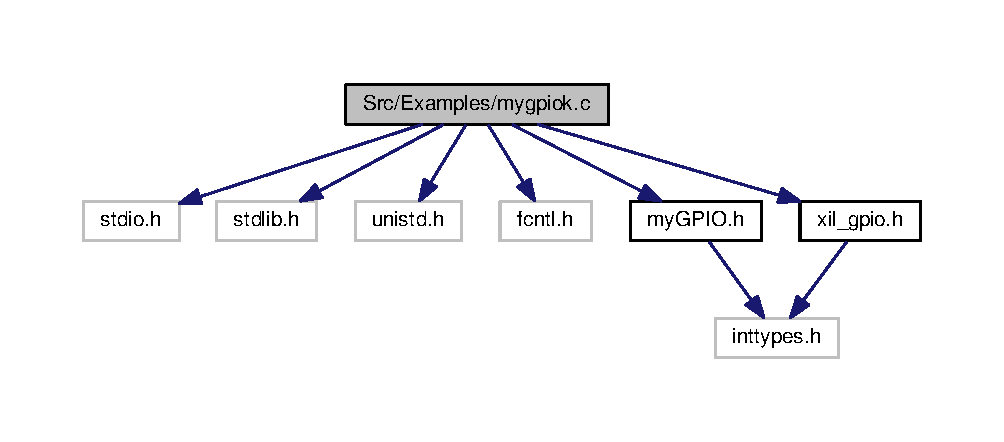
\includegraphics[width=350pt]{mygpiok_8c__incl}
\end{center}
\end{figure}
\subsection*{Strutture dati}
\begin{DoxyCompactItemize}
\item 
struct \hyperlink{structparam__t}{param\+\_\+t}
\begin{DoxyCompactList}\small\item\em La struttura raccoglie tutti i parametri di esecuzione del programma. \end{DoxyCompactList}\end{DoxyCompactItemize}
\subsection*{Definizioni}
\begin{DoxyCompactItemize}
\item 
\#define \hyperlink{mygpiok_8c_a7a63b24ca5489eb3206598e3d90fe19c}{M\+O\+D\+E\+\_\+\+O\+F\+F\+S\+E\+T}~\hyperlink{group__bare-metal_ga81a662103d6ed053978c0a9b4c273065}{my\+G\+P\+I\+O\+\_\+\+M\+O\+D\+E\+\_\+\+O\+F\+F\+S\+E\+T}
\item 
\#define \hyperlink{mygpiok_8c_a77d96306ed0e813f93c4c3f98b970b86}{W\+R\+I\+T\+E\+\_\+\+O\+F\+F\+S\+E\+T}~\hyperlink{group__bare-metal_ga2e45778b6ca9ce6f5768b3f7a4557ce1}{my\+G\+P\+I\+O\+\_\+\+W\+R\+I\+T\+E\+\_\+\+O\+F\+F\+S\+E\+T}
\item 
\#define \hyperlink{mygpiok_8c_ad32c3a5b42163e171daccde5b5d5de02}{R\+E\+A\+D\+\_\+\+O\+F\+F\+S\+E\+T}~\hyperlink{group__bare-metal_ga584d2dfece76e5762030d918d80592cc}{my\+G\+P\+I\+O\+\_\+\+R\+E\+A\+D\+\_\+\+O\+F\+F\+S\+E\+T}
\end{DoxyCompactItemize}
\subsection*{Funzioni}
\begin{DoxyCompactItemize}
\item 
void \hyperlink{mygpiok_8c_a05909651fa170a63e98e3f8e13451b7b}{howto} (void)
\begin{DoxyCompactList}\small\item\em Stampa un messaggio che fornisce indicazioni sull'utilizzo del programma. \end{DoxyCompactList}\item 
int \hyperlink{mygpiok_8c_a65d977fb03a14dedd76e1515d6d24ff4}{parse\+\_\+args} (int argc, char $\ast$$\ast$argv, \hyperlink{structparam__t}{param\+\_\+t} $\ast$param)
\begin{DoxyCompactList}\small\item\em Effettua il parsing dei parametri passati al programma. \end{DoxyCompactList}\item 
void \hyperlink{mygpiok_8c_a63fab82d87963c07f9557a5f5d5d3e86}{gpio\+\_\+op} (\hyperlink{structparam__t}{param\+\_\+t} $\ast$param)
\begin{DoxyCompactList}\small\item\em Effettua operazioni su un device. \end{DoxyCompactList}\item 
int \hyperlink{mygpiok_8c_a3c04138a5bfe5d72780bb7e82a18e627}{main} (int argc, char $\ast$$\ast$argv)
\end{DoxyCompactItemize}


\subsection{Documentazione delle definizioni}
\hypertarget{mygpiok_8c_a7a63b24ca5489eb3206598e3d90fe19c}{\index{mygpiok.\+c@{mygpiok.\+c}!M\+O\+D\+E\+\_\+\+O\+F\+F\+S\+E\+T@{M\+O\+D\+E\+\_\+\+O\+F\+F\+S\+E\+T}}
\index{M\+O\+D\+E\+\_\+\+O\+F\+F\+S\+E\+T@{M\+O\+D\+E\+\_\+\+O\+F\+F\+S\+E\+T}!mygpiok.\+c@{mygpiok.\+c}}
\subsubsection[{M\+O\+D\+E\+\_\+\+O\+F\+F\+S\+E\+T}]{\setlength{\rightskip}{0pt plus 5cm}\#define M\+O\+D\+E\+\_\+\+O\+F\+F\+S\+E\+T~{\bf my\+G\+P\+I\+O\+\_\+\+M\+O\+D\+E\+\_\+\+O\+F\+F\+S\+E\+T}}}\label{mygpiok_8c_a7a63b24ca5489eb3206598e3d90fe19c}
\begin{Desc}
\item[Esempi\+: ]\par
\hyperlink{mygpiok_8c-example}{mygpiok.\+c}, \hyperlink{no_driver_8c-example}{no\+Driver.\+c}, e \hyperlink{uio_8c-example}{uio.\+c}.\end{Desc}
\hypertarget{mygpiok_8c_ad32c3a5b42163e171daccde5b5d5de02}{\index{mygpiok.\+c@{mygpiok.\+c}!R\+E\+A\+D\+\_\+\+O\+F\+F\+S\+E\+T@{R\+E\+A\+D\+\_\+\+O\+F\+F\+S\+E\+T}}
\index{R\+E\+A\+D\+\_\+\+O\+F\+F\+S\+E\+T@{R\+E\+A\+D\+\_\+\+O\+F\+F\+S\+E\+T}!mygpiok.\+c@{mygpiok.\+c}}
\subsubsection[{R\+E\+A\+D\+\_\+\+O\+F\+F\+S\+E\+T}]{\setlength{\rightskip}{0pt plus 5cm}\#define R\+E\+A\+D\+\_\+\+O\+F\+F\+S\+E\+T~{\bf my\+G\+P\+I\+O\+\_\+\+R\+E\+A\+D\+\_\+\+O\+F\+F\+S\+E\+T}}}\label{mygpiok_8c_ad32c3a5b42163e171daccde5b5d5de02}
\begin{Desc}
\item[Esempi\+: ]\par
\hyperlink{mygpiok_8c-example}{mygpiok.\+c}, \hyperlink{no_driver_8c-example}{no\+Driver.\+c}, e \hyperlink{uio_8c-example}{uio.\+c}.\end{Desc}
\hypertarget{mygpiok_8c_a77d96306ed0e813f93c4c3f98b970b86}{\index{mygpiok.\+c@{mygpiok.\+c}!W\+R\+I\+T\+E\+\_\+\+O\+F\+F\+S\+E\+T@{W\+R\+I\+T\+E\+\_\+\+O\+F\+F\+S\+E\+T}}
\index{W\+R\+I\+T\+E\+\_\+\+O\+F\+F\+S\+E\+T@{W\+R\+I\+T\+E\+\_\+\+O\+F\+F\+S\+E\+T}!mygpiok.\+c@{mygpiok.\+c}}
\subsubsection[{W\+R\+I\+T\+E\+\_\+\+O\+F\+F\+S\+E\+T}]{\setlength{\rightskip}{0pt plus 5cm}\#define W\+R\+I\+T\+E\+\_\+\+O\+F\+F\+S\+E\+T~{\bf my\+G\+P\+I\+O\+\_\+\+W\+R\+I\+T\+E\+\_\+\+O\+F\+F\+S\+E\+T}}}\label{mygpiok_8c_a77d96306ed0e813f93c4c3f98b970b86}
\begin{Desc}
\item[Esempi\+: ]\par
\hyperlink{mygpiok_8c-example}{mygpiok.\+c}, \hyperlink{no_driver_8c-example}{no\+Driver.\+c}, e \hyperlink{uio_8c-example}{uio.\+c}.\end{Desc}


\subsection{Documentazione delle funzioni}
\hypertarget{mygpiok_8c_a63fab82d87963c07f9557a5f5d5d3e86}{\index{mygpiok.\+c@{mygpiok.\+c}!gpio\+\_\+op@{gpio\+\_\+op}}
\index{gpio\+\_\+op@{gpio\+\_\+op}!mygpiok.\+c@{mygpiok.\+c}}
\subsubsection[{gpio\+\_\+op}]{\setlength{\rightskip}{0pt plus 5cm}void gpio\+\_\+op (
\begin{DoxyParamCaption}
\item[{{\bf param\+\_\+t} $\ast$}]{param}
\end{DoxyParamCaption}
)}}\label{mygpiok_8c_a63fab82d87963c07f9557a5f5d5d3e86}


Effettua operazioni su un device. 


\begin{DoxyParams}[1]{Parametri}
\mbox{\tt in}  & {\em param} & puntatore a struttura \hyperlink{structparam__t}{param\+\_\+t}, contiene i vari parametri di esecuzione del programma.\\
\hline
\end{DoxyParams}
La funzione viene invocata dopo che sia stato eseguito il parsing dei parametri passati al programma quando esso viene invocato. è stata scritta per funzionare sia con il G\+P\+I\+O Xilinx che con il G\+P\+I\+O custom my\+G\+P\+I\+O. è possibile utilizzare il primo definendo la macro {\bfseries X\+I\+L\+\_\+\+G\+P\+I\+O}. Effettua, sul device, le operazioni impostate, in accordo con i parametri passati al programma alla sua invocazione. ~\newline
 Nel caso un cui si usi un driver ad-\/hoc, è possibile usare le funzioni read() e write() per interagire con il device, leggendo il valore dei registri o scrivendolo. Il driver my\+G\+P\+I\+O\+K mette a disposizione anche la funzione seek() che permette di scegliere quale registro leggere o scrivere. \subparagraph*{Impostazione della modalità di funzionamento}

Per impostare la modalità di funzionamento è necessario scrivere sul registro M\+O\+D\+E. L'offset di tale registro è determinato in base al particolare device che si stà utilizzando. Dopo aver spostato la \char`\"{}testina di scrittura\char`\"{} sul registro M\+O\+D\+E usando la funzione seek(), viene effettuata la scrittura su di esso usando la funzione write(). è possibile, definendo la macro {\bfseries U\+S\+E\+\_\+\+P\+W\+R\+I\+T\+E}, usare la funzione pwrite(), che combina le due operazioni.

\subparagraph*{Operazione di scrittura}

Per impostare il valore dei pin del device è necessario scrivere sul registro W\+R\+I\+T\+E. L'offset di tale registro è determinato in base al particolare device che si stà utilizzando. Dopo aver spostato la \char`\"{}testina di scrittura\char`\"{} sul registro W\+R\+I\+T\+E usando la funzione seek(), viene effettuata la scrittura su di esso usando la funzione write(). è possibile, definendo la macro {\bfseries U\+S\+E\+\_\+\+P\+W\+R\+I\+T\+E}, usare la funzione pwrite(), che combina le due operazioni.

\subparagraph*{Operazione di lettura con interrupt}

La lettura dei pin del device avviene mediante la chiamata alla funzione read(), dopo aver spostato la \char`\"{}testina di lettura\char`\"{} sul registro R\+E\+A\+D. L'offset di tale registro, come nei due casi precedenti, viene determinato in base al particolare device che si sta usando. è possibile, definendo la macro {\bfseries U\+S\+E\+\_\+\+P\+R\+E\+A\+D}, usare la funzione pread(), che combina le operazioni di seek() e read(). Il driver my\+G\+P\+I\+O\+K implementa un meccanismo di lettura bloccante\+: qualora non ci siano dati disponibili, il processo che chiama read() viene sospeso e messo in attesa che i dati siano disponibili. Quando arriva una interruzione dal device, il driver my\+G\+P\+I\+O\+K lo gestisce e risveglia i processi che erano stati messi precedentemente in attesa. Si legga la documentazione del driver my\+G\+P\+I\+O\+K per i dettagli.\begin{Desc}
\item[Esempi\+: ]\par
\hyperlink{mygpiok_8c-example}{mygpiok.\+c}.\end{Desc}
\hypertarget{mygpiok_8c_a05909651fa170a63e98e3f8e13451b7b}{\index{mygpiok.\+c@{mygpiok.\+c}!howto@{howto}}
\index{howto@{howto}!mygpiok.\+c@{mygpiok.\+c}}
\subsubsection[{howto}]{\setlength{\rightskip}{0pt plus 5cm}void howto (
\begin{DoxyParamCaption}
\item[{void}]{}
\end{DoxyParamCaption}
)}}\label{mygpiok_8c_a05909651fa170a63e98e3f8e13451b7b}


Stampa un messaggio che fornisce indicazioni sull'utilizzo del programma. 

\begin{Desc}
\item[Esempi\+: ]\par
\hyperlink{mygpiok_8c-example}{mygpiok.\+c}.\end{Desc}
\hypertarget{mygpiok_8c_a3c04138a5bfe5d72780bb7e82a18e627}{\index{mygpiok.\+c@{mygpiok.\+c}!main@{main}}
\index{main@{main}!mygpiok.\+c@{mygpiok.\+c}}
\subsubsection[{main}]{\setlength{\rightskip}{0pt plus 5cm}int main (
\begin{DoxyParamCaption}
\item[{int}]{argc, }
\item[{char $\ast$$\ast$}]{argv}
\end{DoxyParamCaption}
)}}\label{mygpiok_8c_a3c04138a5bfe5d72780bb7e82a18e627}
\begin{Desc}
\item[Esempi\+: ]\par
\hyperlink{mygpiok_8c-example}{mygpiok.\+c}.\end{Desc}
\hypertarget{mygpiok_8c_a65d977fb03a14dedd76e1515d6d24ff4}{\index{mygpiok.\+c@{mygpiok.\+c}!parse\+\_\+args@{parse\+\_\+args}}
\index{parse\+\_\+args@{parse\+\_\+args}!mygpiok.\+c@{mygpiok.\+c}}
\subsubsection[{parse\+\_\+args}]{\setlength{\rightskip}{0pt plus 5cm}int parse\+\_\+args (
\begin{DoxyParamCaption}
\item[{int}]{argc, }
\item[{char $\ast$$\ast$}]{argv, }
\item[{{\bf param\+\_\+t} $\ast$}]{param}
\end{DoxyParamCaption}
)}}\label{mygpiok_8c_a65d977fb03a14dedd76e1515d6d24ff4}


Effettua il parsing dei parametri passati al programma. 


\begin{DoxyParams}[1]{Parametri}
\mbox{\tt in}  & {\em argc} & \\
\hline
\mbox{\tt in}  & {\em argv} & \\
\hline
\mbox{\tt out}  & {\em param} & puntatore a struttura \hyperlink{structparam__t}{param\+\_\+t}, conterrà i vari parametri di esecuzione del programma.\\
\hline
\end{DoxyParams}

\begin{DoxyRetVals}{Valori di ritorno}
{\em 0} & se il parsing ha successo \\
\hline
{\em -\/1} & se si verifica un errore \\
\hline
\end{DoxyRetVals}
\subparagraph*{Parsing dei parametri del programma.}

Il parsing viene effettuato usando la funzione getopt(). 
\begin{DoxyCode}
1 #include <unistd.h>
2 int getopt(int argc, char * const argv[], const char *optstring);
\end{DoxyCode}
 Essa prende in input i parametri argc ed argv passati alla funzione \hyperlink{mygpiok_8c_a3c04138a5bfe5d72780bb7e82a18e627}{main()} quando il programma viene invocato. Quando una delle stringhe che compongono argv comincia con il carattere '-\/', getopt() la considera una opzione. Il carattere immediatamente successivo il '-\/' identifica la particolare opzione. La funzione può essere chiamata ripetutamente, fino a quando non restituisce -\/1, ad indicare che sono stati analizzati tutti i parametri passati al programma. Quando getopt() trova un'opzione, restituisce quel carattere ed aggiorna la variabile globale optind, che punta al prossimo parametro contenuto in argv. La stringa optstring indica quali sono le opzioni considerate. Se una opzione è seguita da '\+:' vuol dire che essa è seguita da un argomento. Tale argomento può essere ottenuto mediante la variabile globale optarg.

\subparagraph*{Parametri riconosciuti}

La funzione riconosce i parametri\+:
\begin{DoxyItemize}
\item 'd' \+: seguito dal percorso del device /dev/my\+G\+P\+I\+O\+K col quale interagire
\item 'w' \+: operazione di scrittura, seguito dal valore che si intende scrivere, in esadecimale; la scrittura verrà effettuata sul registro W\+R\+I\+T\+E;
\item 'm' \+: impostazione modalità, seguito dalla modalità col quale impostare il device; la scrittura verrà effettuata sul registro M\+O\+D\+E;
\item 'r' \+: operazione di lettura, primo di argomento; la lettura viene effettuata dal registro R\+E\+A\+D ed è non bloccante, nel senso che viene semplicemente letto il contenuto del registro.
\end{DoxyItemize}

Se non viene specificato il device my\+G\+P\+I\+O\+K col quale interagire è impossibile continuare. Per questo motivo, in questo caso, la funzione restituisce -\/1, per cui il programma viene terminato.\begin{Desc}
\item[Esempi\+: ]\par
\hyperlink{mygpiok_8c-example}{mygpiok.\+c}.\end{Desc}

\hypertarget{no_driver_8c}{\section{Riferimenti per il file my\+G\+P\+I\+O/linux-\/driver/no\+Driver.c}
\label{no_driver_8c}\index{my\+G\+P\+I\+O/linux-\/driver/no\+Driver.\+c@{my\+G\+P\+I\+O/linux-\/driver/no\+Driver.\+c}}
}
{\ttfamily \#include $<$inttypes.\+h$>$}\\*
{\ttfamily \#include $<$stdio.\+h$>$}\\*
{\ttfamily \#include $<$stdlib.\+h$>$}\\*
{\ttfamily \#include $<$unistd.\+h$>$}\\*
{\ttfamily \#include $<$sys/mman.\+h$>$}\\*
{\ttfamily \#include $<$fcntl.\+h$>$}\\*
{\ttfamily \#include \char`\"{}my\+G\+P\+I\+O.\+h\char`\"{}}\\*
Grafo delle dipendenze di inclusione per no\+Driver.\+c\+:\nopagebreak
\begin{figure}[H]
\begin{center}
\leavevmode
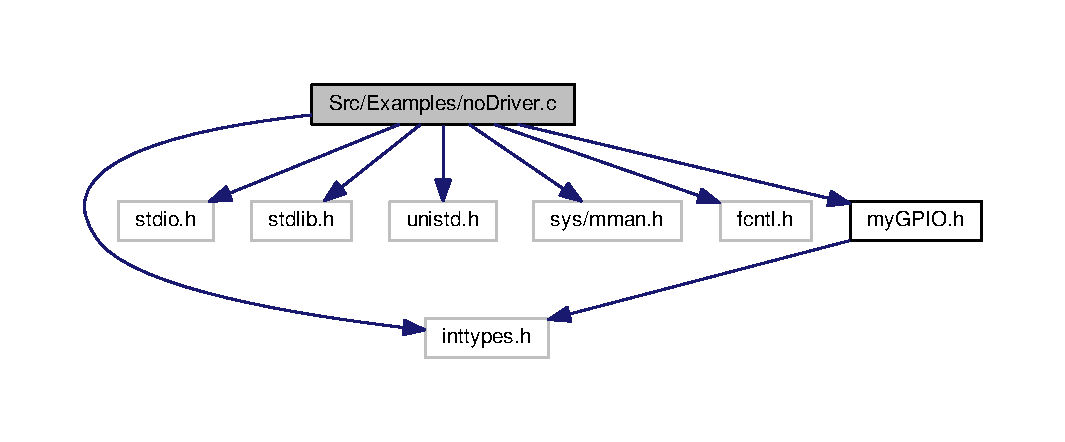
\includegraphics[width=350pt]{no_driver_8c__incl}
\end{center}
\end{figure}
\subsection*{Funzioni}
\begin{DoxyCompactItemize}
\item 
void \hyperlink{group___no_driver_ga05909651fa170a63e98e3f8e13451b7b}{howto} (void)
\begin{DoxyCompactList}\small\item\em Stampa un messaggio che fornisce indicazioni sull'utilizzo del programma. \end{DoxyCompactList}\item 
int \hyperlink{group___no_driver_ga218f8a9dfc36572bfe2230c5e2d2c776}{parse\+\_\+args} (int argc, char $\ast$$\ast$argv, uint32\+\_\+t $\ast$gpio\+\_\+address, uint8\+\_\+t $\ast$op\+\_\+mode, uint32\+\_\+t $\ast$mode\+\_\+value, uint8\+\_\+t $\ast$op\+\_\+write, uint32\+\_\+t $\ast$write\+\_\+value, uint8\+\_\+t $\ast$op\+\_\+read)
\begin{DoxyCompactList}\small\item\em Effettua il parsing dei parametri passati al programma. \end{DoxyCompactList}\item 
void \hyperlink{group___no_driver_ga879d8b839631449ecb5bc4d0721432b6}{gpio\+\_\+op} (void $\ast$vrt\+\_\+gpio\+\_\+addr, uint8\+\_\+t op\+\_\+mode, uint32\+\_\+t mode\+\_\+value, uint8\+\_\+t op\+\_\+write, uint32\+\_\+t write\+\_\+value, uint8\+\_\+t op\+\_\+read)
\begin{DoxyCompactList}\small\item\em Effettua operazioni su un device. \end{DoxyCompactList}\item 
int \hyperlink{group___no_driver_ga3c04138a5bfe5d72780bb7e82a18e627}{main} (int argc, char $\ast$$\ast$argv)
\end{DoxyCompactItemize}


\subsection{Descrizione dettagliata}
\begin{DoxyAuthor}{Autore}
Salvatore Barone \href{mailto:salvator.barone@gmail.com}{\tt salvator.\+barone@gmail.\+com} 
\end{DoxyAuthor}
\begin{DoxyDate}{Data}
12 06 2017
\end{DoxyDate}
\begin{DoxyCopyright}{Copyright}
Copyright 2017 Salvatore Barone \href{mailto:salvator.barone@gmail.com}{\tt salvator.\+barone@gmail.\+com}
\end{DoxyCopyright}
This file is part of Zynq7000\+Driver\+Pack

Zynq7000\+Driver\+Pack is free software; you can redistribute it and/or modify it under the terms of the G\+N\+U General Public License as published by the Free Software Foundation; either version 3 of the License, or any later version.

Zynq7000\+Driver\+Pack is distributed in the hope that it will be useful, but W\+I\+T\+H\+O\+U\+T A\+N\+Y W\+A\+R\+R\+A\+N\+T\+Y; without even the implied warranty of M\+E\+R\+C\+H\+A\+N\+T\+A\+B\+I\+L\+I\+T\+Y or F\+I\+T\+N\+E\+S\+S F\+O\+R A P\+A\+R\+T\+I\+C\+U\+L\+A\+R P\+U\+R\+P\+O\+S\+E. See the G\+N\+U General Public License for more details.

You should have received a copy of the G\+N\+U General Public License along with this program; if not, write to the Free Software Foundation, Inc., 51 Franklin Street, Fifth Floor, Boston, M\+A 02110-\/1301, U\+S\+A. 
\hypertarget{read_all_8c}{\section{Riferimenti per il file Src/\+Examples/read\+All.c}
\label{read_all_8c}\index{Src/\+Examples/read\+All.\+c@{Src/\+Examples/read\+All.\+c}}
}
{\ttfamily \#include $<$inttypes.\+h$>$}\\*
{\ttfamily \#include $<$stdio.\+h$>$}\\*
{\ttfamily \#include $<$stdlib.\+h$>$}\\*
{\ttfamily \#include $<$unistd.\+h$>$}\\*
{\ttfamily \#include $<$sys/mman.\+h$>$}\\*
{\ttfamily \#include $<$fcntl.\+h$>$}\\*
Grafo delle dipendenze di inclusione per read\+All.\+c\+:\nopagebreak
\begin{figure}[H]
\begin{center}
\leavevmode
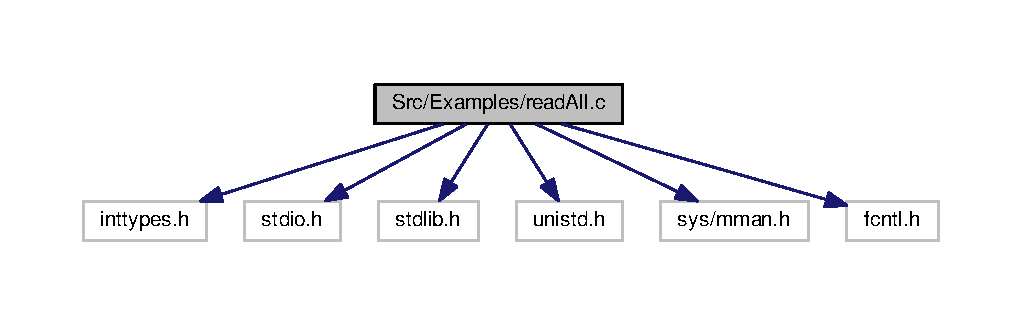
\includegraphics[width=350pt]{read_all_8c__incl}
\end{center}
\end{figure}
\subsection*{Funzioni}
\begin{DoxyCompactItemize}
\item 
void \hyperlink{read_all_8c_a05909651fa170a63e98e3f8e13451b7b}{howto} (void)
\item 
int \hyperlink{read_all_8c_a87c1177178432113628b0885b0cff1b2}{parse\+\_\+args} (int argc, char $\ast$$\ast$argv, uint32\+\_\+t $\ast$gpio\+\_\+address, uint32\+\_\+t $\ast$max\+\_\+offset)
\item 
int \hyperlink{read_all_8c_a3c04138a5bfe5d72780bb7e82a18e627}{main} (int argc, char $\ast$$\ast$argv)
\end{DoxyCompactItemize}


\subsection{Documentazione delle funzioni}
\hypertarget{read_all_8c_a05909651fa170a63e98e3f8e13451b7b}{\index{read\+All.\+c@{read\+All.\+c}!howto@{howto}}
\index{howto@{howto}!read\+All.\+c@{read\+All.\+c}}
\subsubsection[{howto}]{\setlength{\rightskip}{0pt plus 5cm}void howto (
\begin{DoxyParamCaption}
\item[{void}]{}
\end{DoxyParamCaption}
)}}\label{read_all_8c_a05909651fa170a63e98e3f8e13451b7b}
\begin{Desc}
\item[Esempi\+: ]\par
\hyperlink{read_all_8c-example}{read\+All.\+c}.\end{Desc}
\hypertarget{read_all_8c_a3c04138a5bfe5d72780bb7e82a18e627}{\index{read\+All.\+c@{read\+All.\+c}!main@{main}}
\index{main@{main}!read\+All.\+c@{read\+All.\+c}}
\subsubsection[{main}]{\setlength{\rightskip}{0pt plus 5cm}int main (
\begin{DoxyParamCaption}
\item[{int}]{argc, }
\item[{char $\ast$$\ast$}]{argv}
\end{DoxyParamCaption}
)}}\label{read_all_8c_a3c04138a5bfe5d72780bb7e82a18e627}
\begin{Desc}
\item[Esempi\+: ]\par
\hyperlink{read_all_8c-example}{read\+All.\+c}.\end{Desc}
\hypertarget{read_all_8c_a87c1177178432113628b0885b0cff1b2}{\index{read\+All.\+c@{read\+All.\+c}!parse\+\_\+args@{parse\+\_\+args}}
\index{parse\+\_\+args@{parse\+\_\+args}!read\+All.\+c@{read\+All.\+c}}
\subsubsection[{parse\+\_\+args}]{\setlength{\rightskip}{0pt plus 5cm}int parse\+\_\+args (
\begin{DoxyParamCaption}
\item[{int}]{argc, }
\item[{char $\ast$$\ast$}]{argv, }
\item[{uint32\+\_\+t $\ast$}]{gpio\+\_\+address, }
\item[{uint32\+\_\+t $\ast$}]{max\+\_\+offset}
\end{DoxyParamCaption}
)}}\label{read_all_8c_a87c1177178432113628b0885b0cff1b2}
\begin{Desc}
\item[Esempi\+: ]\par
\hyperlink{read_all_8c-example}{read\+All.\+c}.\end{Desc}

\hypertarget{uio-int_8c}{\section{Riferimenti per il file my\+G\+P\+I\+O/linux-\/driver/uio-\/int.c}
\label{uio-int_8c}\index{my\+G\+P\+I\+O/linux-\/driver/uio-\/int.\+c@{my\+G\+P\+I\+O/linux-\/driver/uio-\/int.\+c}}
}
{\ttfamily \#include $<$inttypes.\+h$>$}\\*
{\ttfamily \#include $<$stdio.\+h$>$}\\*
{\ttfamily \#include $<$stdlib.\+h$>$}\\*
{\ttfamily \#include $<$unistd.\+h$>$}\\*
{\ttfamily \#include $<$sys/mman.\+h$>$}\\*
{\ttfamily \#include $<$fcntl.\+h$>$}\\*
{\ttfamily \#include \char`\"{}my\+G\+P\+I\+O.\+h\char`\"{}}\\*
{\ttfamily \#include \char`\"{}xil\+\_\+gpio.\+h\char`\"{}}\\*
Grafo delle dipendenze di inclusione per uio-\/int.c\+:\nopagebreak
\begin{figure}[H]
\begin{center}
\leavevmode
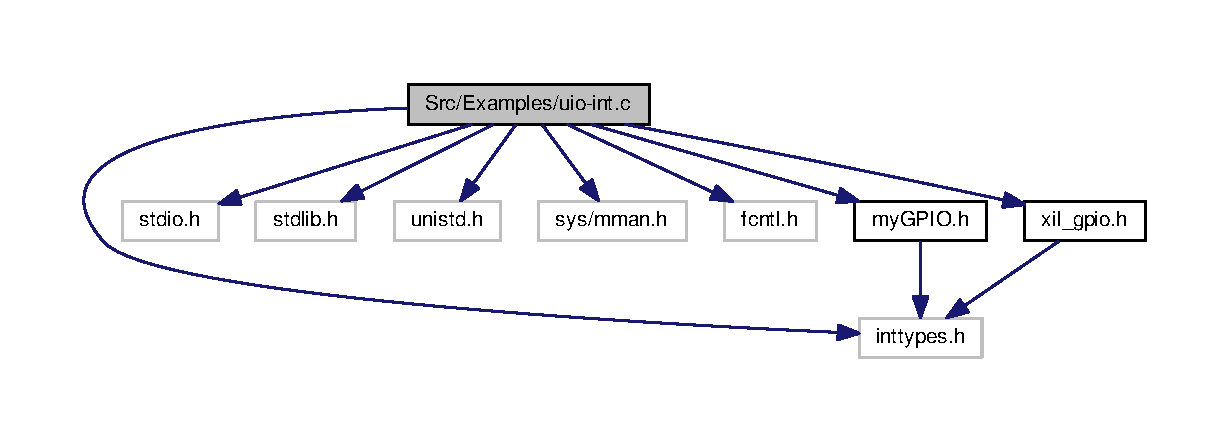
\includegraphics[width=350pt]{uio-int_8c__incl}
\end{center}
\end{figure}
\subsection*{Funzioni}
\begin{DoxyCompactItemize}
\item 
void \hyperlink{group___u_i_o-interrupt_ga05909651fa170a63e98e3f8e13451b7b}{howto} (void)
\begin{DoxyCompactList}\small\item\em Stampa un messaggio che fornisce indicazioni sull'utilizzo del programma. \end{DoxyCompactList}\item 
int \hyperlink{group___u_i_o-interrupt_ga15f7e5adb83963e5d21ccea3186b5364}{parse\+\_\+args} (int argc, char $\ast$$\ast$argv, char $\ast$$\ast$uio\+\_\+file, uint8\+\_\+t $\ast$op\+\_\+mode, uint32\+\_\+t $\ast$mode\+\_\+value, uint8\+\_\+t $\ast$op\+\_\+write, uint32\+\_\+t $\ast$write\+\_\+value, uint8\+\_\+t $\ast$op\+\_\+read)
\begin{DoxyCompactList}\small\item\em Effettua il parsing dei parametri passati al programma. \end{DoxyCompactList}\item 
void \hyperlink{group___u_i_o-interrupt_ga78b676750c5d08c316cad35ec3963c53}{gpio\+\_\+op} (void $\ast$vrt\+\_\+gpio\+\_\+addr, int uio\+\_\+descriptor, uint8\+\_\+t op\+\_\+mode, uint32\+\_\+t mode\+\_\+value, uint8\+\_\+t op\+\_\+write, uint32\+\_\+t write\+\_\+value, uint8\+\_\+t op\+\_\+read)
\begin{DoxyCompactList}\small\item\em Effettua operazioni su un device. \end{DoxyCompactList}\item 
int \hyperlink{group___u_i_o-interrupt_ga3c04138a5bfe5d72780bb7e82a18e627}{main} (int argc, char $\ast$$\ast$argv)
\end{DoxyCompactItemize}


\subsection{Descrizione dettagliata}
\begin{DoxyAuthor}{Autore}
Salvatore Barone \href{mailto:salvator.barone@gmail.com}{\tt salvator.\+barone@gmail.\+com} 
\end{DoxyAuthor}
\begin{DoxyDate}{Data}
14 06 2017
\end{DoxyDate}
\begin{DoxyCopyright}{Copyright}
Copyright 2017 Salvatore Barone \href{mailto:salvator.barone@gmail.com}{\tt salvator.\+barone@gmail.\+com}
\end{DoxyCopyright}
This file is part of Zynq7000\+Driver\+Pack

Zynq7000\+Driver\+Pack is free software; you can redistribute it and/or modify it under the terms of the G\+N\+U General Public License as published by the Free Software Foundation; either version 3 of the License, or any later version.

Zynq7000\+Driver\+Pack is distributed in the hope that it will be useful, but W\+I\+T\+H\+O\+U\+T A\+N\+Y W\+A\+R\+R\+A\+N\+T\+Y; without even the implied warranty of M\+E\+R\+C\+H\+A\+N\+T\+A\+B\+I\+L\+I\+T\+Y or F\+I\+T\+N\+E\+S\+S F\+O\+R A P\+A\+R\+T\+I\+C\+U\+L\+A\+R P\+U\+R\+P\+O\+S\+E. See the G\+N\+U General Public License for more details.

You should have received a copy of the G\+N\+U General Public License along with this program; if not, write to the Free Software Foundation, Inc., 51 Franklin Street, Fifth Floor, Boston, M\+A 02110-\/1301, U\+S\+A. 
\hypertarget{uio_8c}{\section{Riferimenti per il file my\+G\+P\+I\+O/linux-\/driver/uio.c}
\label{uio_8c}\index{my\+G\+P\+I\+O/linux-\/driver/uio.\+c@{my\+G\+P\+I\+O/linux-\/driver/uio.\+c}}
}
{\ttfamily \#include $<$inttypes.\+h$>$}\\*
{\ttfamily \#include $<$stdio.\+h$>$}\\*
{\ttfamily \#include $<$stdlib.\+h$>$}\\*
{\ttfamily \#include $<$unistd.\+h$>$}\\*
{\ttfamily \#include $<$sys/mman.\+h$>$}\\*
{\ttfamily \#include $<$fcntl.\+h$>$}\\*
{\ttfamily \#include \char`\"{}my\+G\+P\+I\+O.\+h\char`\"{}}\\*
Grafo delle dipendenze di inclusione per uio.\+c\+:\nopagebreak
\begin{figure}[H]
\begin{center}
\leavevmode
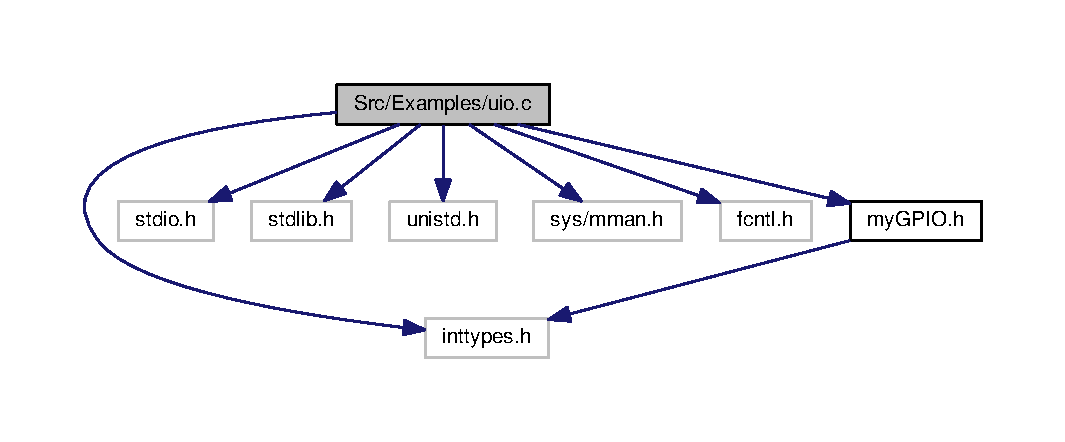
\includegraphics[width=350pt]{uio_8c__incl}
\end{center}
\end{figure}
\subsection*{Funzioni}
\begin{DoxyCompactItemize}
\item 
void \hyperlink{group___u_i_o-simple_ga05909651fa170a63e98e3f8e13451b7b}{howto} (void)
\begin{DoxyCompactList}\small\item\em Stampa un messaggio che fornisce indicazioni sull'utilizzo del programma. \end{DoxyCompactList}\item 
int \hyperlink{group___u_i_o-simple_ga15f7e5adb83963e5d21ccea3186b5364}{parse\+\_\+args} (int argc, char $\ast$$\ast$argv, char $\ast$$\ast$uio\+\_\+file, uint8\+\_\+t $\ast$op\+\_\+mode, uint32\+\_\+t $\ast$mode\+\_\+value, uint8\+\_\+t $\ast$op\+\_\+write, uint32\+\_\+t $\ast$write\+\_\+value, uint8\+\_\+t $\ast$op\+\_\+read)
\begin{DoxyCompactList}\small\item\em Effettua il parsing dei parametri passati al programma. \end{DoxyCompactList}\item 
void \hyperlink{group___u_i_o-simple_ga879d8b839631449ecb5bc4d0721432b6}{gpio\+\_\+op} (void $\ast$vrt\+\_\+gpio\+\_\+addr, uint8\+\_\+t op\+\_\+mode, uint32\+\_\+t mode\+\_\+value, uint8\+\_\+t op\+\_\+write, uint32\+\_\+t write\+\_\+value, uint8\+\_\+t op\+\_\+read)
\begin{DoxyCompactList}\small\item\em Effettua operazioni su un device. \end{DoxyCompactList}\item 
int \hyperlink{group___u_i_o-simple_ga3c04138a5bfe5d72780bb7e82a18e627}{main} (int argc, char $\ast$$\ast$argv)
\end{DoxyCompactItemize}


\subsection{Descrizione dettagliata}
\begin{DoxyAuthor}{Autore}
Salvatore Barone \href{mailto:salvator.barone@gmail.com}{\tt salvator.\+barone@gmail.\+com} 
\end{DoxyAuthor}
\begin{DoxyDate}{Data}
13 06 2017
\end{DoxyDate}
\begin{DoxyCopyright}{Copyright}
Copyright 2017 Salvatore Barone \href{mailto:salvator.barone@gmail.com}{\tt salvator.\+barone@gmail.\+com}
\end{DoxyCopyright}
This file is part of Zynq7000\+Driver\+Pack

Zynq7000\+Driver\+Pack is free software; you can redistribute it and/or modify it under the terms of the G\+N\+U General Public License as published by the Free Software Foundation; either version 3 of the License, or any later version.

Zynq7000\+Driver\+Pack is distributed in the hope that it will be useful, but W\+I\+T\+H\+O\+U\+T A\+N\+Y W\+A\+R\+R\+A\+N\+T\+Y; without even the implied warranty of M\+E\+R\+C\+H\+A\+N\+T\+A\+B\+I\+L\+I\+T\+Y or F\+I\+T\+N\+E\+S\+S F\+O\+R A P\+A\+R\+T\+I\+C\+U\+L\+A\+R P\+U\+R\+P\+O\+S\+E. See the G\+N\+U General Public License for more details.

You should have received a copy of the G\+N\+U General Public License along with this program; if not, write to the Free Software Foundation, Inc., 51 Franklin Street, Fifth Floor, Boston, M\+A 02110-\/1301, U\+S\+A. 
\hypertarget{xil__gpio_8c}{\section{Riferimenti per il file Src/\+Examples/xil\+\_\+gpio.c}
\label{xil__gpio_8c}\index{Src/\+Examples/xil\+\_\+gpio.\+c@{Src/\+Examples/xil\+\_\+gpio.\+c}}
}
{\ttfamily \#include \char`\"{}xil\+\_\+gpio.\+h\char`\"{}}\\*
{\ttfamily \#include $<$stdio.\+h$>$}\\*
Grafo delle dipendenze di inclusione per xil\+\_\+gpio.\+c\+:\nopagebreak
\begin{figure}[H]
\begin{center}
\leavevmode
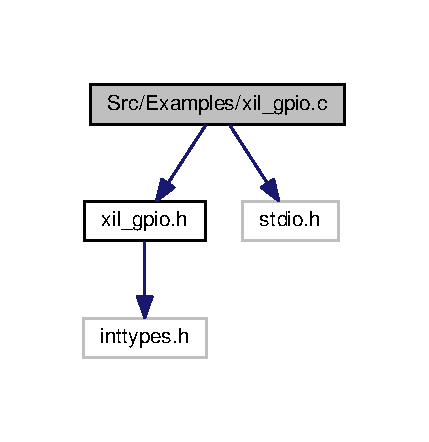
\includegraphics[width=206pt]{xil__gpio_8c__incl}
\end{center}
\end{figure}
\subsection*{Funzioni}
\begin{DoxyCompactItemize}
\item 
int \hyperlink{xil__gpio_8c_aac9ff33f07964a1f5f9b8b1173072d67}{Xil\+Gpio\+\_\+\+Global\+\_\+\+Interrupt} (uint32\+\_\+t $\ast$base\+Address, uint32\+\_\+t mask)
\item 
int \hyperlink{xil__gpio_8c_ab335ddab38389969b7a1fdb226eb1fbf}{Xil\+Gpio\+\_\+\+Channel\+\_\+\+Interrupt} (uint32\+\_\+t $\ast$base\+Address, uint32\+\_\+t mask)
\item 
int \hyperlink{xil__gpio_8c_ad7b9691b1dc24679b60c25a6d5dc9647}{Xil\+Gpio\+\_\+\+Ack\+\_\+\+Interrupt} (uint32\+\_\+t $\ast$base\+Address, uint32\+\_\+t channel)
\end{DoxyCompactItemize}


\subsection{Documentazione delle funzioni}
\hypertarget{xil__gpio_8c_ad7b9691b1dc24679b60c25a6d5dc9647}{\index{xil\+\_\+gpio.\+c@{xil\+\_\+gpio.\+c}!Xil\+Gpio\+\_\+\+Ack\+\_\+\+Interrupt@{Xil\+Gpio\+\_\+\+Ack\+\_\+\+Interrupt}}
\index{Xil\+Gpio\+\_\+\+Ack\+\_\+\+Interrupt@{Xil\+Gpio\+\_\+\+Ack\+\_\+\+Interrupt}!xil\+\_\+gpio.\+c@{xil\+\_\+gpio.\+c}}
\subsubsection[{Xil\+Gpio\+\_\+\+Ack\+\_\+\+Interrupt}]{\setlength{\rightskip}{0pt plus 5cm}int Xil\+Gpio\+\_\+\+Ack\+\_\+\+Interrupt (
\begin{DoxyParamCaption}
\item[{uint32\+\_\+t $\ast$}]{base\+Address, }
\item[{uint32\+\_\+t}]{channel}
\end{DoxyParamCaption}
)}}\label{xil__gpio_8c_ad7b9691b1dc24679b60c25a6d5dc9647}
\hypertarget{xil__gpio_8c_ab335ddab38389969b7a1fdb226eb1fbf}{\index{xil\+\_\+gpio.\+c@{xil\+\_\+gpio.\+c}!Xil\+Gpio\+\_\+\+Channel\+\_\+\+Interrupt@{Xil\+Gpio\+\_\+\+Channel\+\_\+\+Interrupt}}
\index{Xil\+Gpio\+\_\+\+Channel\+\_\+\+Interrupt@{Xil\+Gpio\+\_\+\+Channel\+\_\+\+Interrupt}!xil\+\_\+gpio.\+c@{xil\+\_\+gpio.\+c}}
\subsubsection[{Xil\+Gpio\+\_\+\+Channel\+\_\+\+Interrupt}]{\setlength{\rightskip}{0pt plus 5cm}int Xil\+Gpio\+\_\+\+Channel\+\_\+\+Interrupt (
\begin{DoxyParamCaption}
\item[{uint32\+\_\+t $\ast$}]{base\+Address, }
\item[{uint32\+\_\+t}]{mask}
\end{DoxyParamCaption}
)}}\label{xil__gpio_8c_ab335ddab38389969b7a1fdb226eb1fbf}
\hypertarget{xil__gpio_8c_aac9ff33f07964a1f5f9b8b1173072d67}{\index{xil\+\_\+gpio.\+c@{xil\+\_\+gpio.\+c}!Xil\+Gpio\+\_\+\+Global\+\_\+\+Interrupt@{Xil\+Gpio\+\_\+\+Global\+\_\+\+Interrupt}}
\index{Xil\+Gpio\+\_\+\+Global\+\_\+\+Interrupt@{Xil\+Gpio\+\_\+\+Global\+\_\+\+Interrupt}!xil\+\_\+gpio.\+c@{xil\+\_\+gpio.\+c}}
\subsubsection[{Xil\+Gpio\+\_\+\+Global\+\_\+\+Interrupt}]{\setlength{\rightskip}{0pt plus 5cm}int Xil\+Gpio\+\_\+\+Global\+\_\+\+Interrupt (
\begin{DoxyParamCaption}
\item[{uint32\+\_\+t $\ast$}]{base\+Address, }
\item[{uint32\+\_\+t}]{mask}
\end{DoxyParamCaption}
)}}\label{xil__gpio_8c_aac9ff33f07964a1f5f9b8b1173072d67}

\hypertarget{xil__gpio_8h}{\section{Riferimenti per il file my\+G\+P\+I\+O/linux-\/driver/xil\+\_\+gpio.h}
\label{xil__gpio_8h}\index{my\+G\+P\+I\+O/linux-\/driver/xil\+\_\+gpio.\+h@{my\+G\+P\+I\+O/linux-\/driver/xil\+\_\+gpio.\+h}}
}
{\ttfamily \#include $<$inttypes.\+h$>$}\\*
Grafo delle dipendenze di inclusione per xil\+\_\+gpio.\+h\+:\nopagebreak
\begin{figure}[H]
\begin{center}
\leavevmode
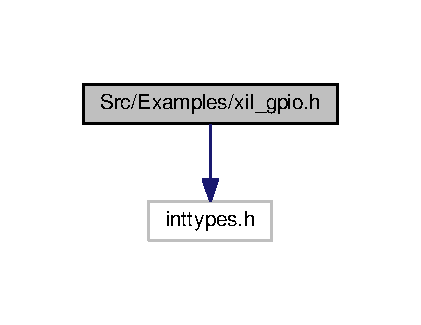
\includegraphics[width=185pt]{xil__gpio_8h__incl}
\end{center}
\end{figure}
Questo grafo mostra quali altri file includono direttamente o indirettamente questo file\+:\nopagebreak
\begin{figure}[H]
\begin{center}
\leavevmode
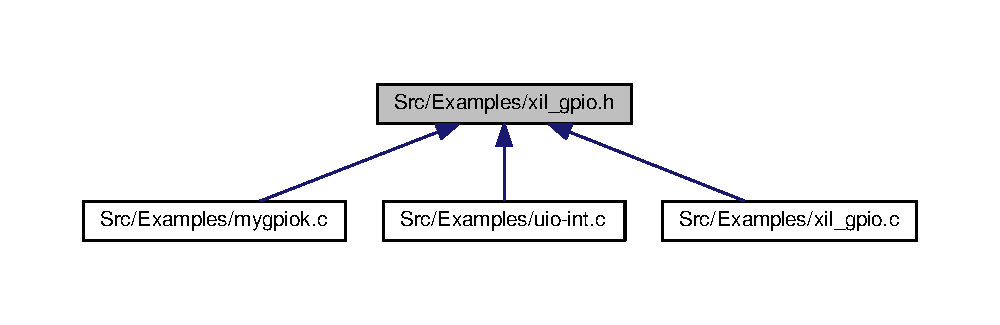
\includegraphics[width=350pt]{xil__gpio_8h__dep__incl}
\end{center}
\end{figure}
\subsection*{Definizioni}
\begin{DoxyCompactItemize}
\item 
\#define \hyperlink{xil__gpio_8h_a0b576e472f8ad06f166d9107de3b0348}{X\+G\+P\+I\+O\+\_\+\+G\+I\+E\+\_\+\+G\+I\+N\+T\+R\+\_\+\+E\+N\+A\+B\+L\+E\+\_\+\+M\+A\+S\+K}~0x80000000
\item 
\#define \hyperlink{xil__gpio_8h_a78907649b00f7076af686bcac4cd1b8c}{G\+P\+I\+O\+\_\+\+D\+A\+T\+A\+\_\+\+O\+F\+F\+S\+E\+T}~0x00
\item 
\#define \hyperlink{xil__gpio_8h_a6e2a77c24e8a4e2b3800085ac10a8cf6}{G\+P\+I\+O\+\_\+\+T\+R\+I\+\_\+\+O\+F\+F\+S\+E\+T}~0x04
\item 
\#define \hyperlink{xil__gpio_8h_ae5cbf47902785bbcc678bddb8212c86b}{G\+P\+I\+O\+\_\+\+R\+E\+A\+D\+\_\+\+O\+F\+F\+S\+E\+T}~0x08
\item 
\#define \hyperlink{xil__gpio_8h_a389241f63fd0ce9af2c1f6dc0f69dcb3}{X\+G\+P\+I\+O\+\_\+\+G\+I\+E\+\_\+\+O\+F\+F\+S\+E\+T}~0x11\+C
\item 
\#define \hyperlink{xil__gpio_8h_a6cbde8210cb1476b67ca87eccacbc2ed}{X\+G\+P\+I\+O\+\_\+\+I\+S\+R\+\_\+\+O\+F\+F\+S\+E\+T}~0x120
\item 
\#define \hyperlink{xil__gpio_8h_a4f62e4ffa9e47cd55133c583134f4f57}{X\+G\+P\+I\+O\+\_\+\+I\+E\+R\+\_\+\+O\+F\+F\+S\+E\+T}~0x128
\item 
\#define \hyperlink{xil__gpio_8h_adede88fc60bf8fc2dd1df41223bcaab2}{G\+L\+O\+B\+A\+L\+\_\+\+I\+N\+T\+R\+\_\+\+E\+N\+A\+B\+L\+E}~\hyperlink{xil__gpio_8h_a0b576e472f8ad06f166d9107de3b0348}{X\+G\+P\+I\+O\+\_\+\+G\+I\+E\+\_\+\+G\+I\+N\+T\+R\+\_\+\+E\+N\+A\+B\+L\+E\+\_\+\+M\+A\+S\+K}
\item 
\#define \hyperlink{xil__gpio_8h_a130274e8d50b05c49c171bde017762f8}{C\+H\+A\+N\+N\+E\+L1\+\_\+\+I\+N\+T\+R\+\_\+\+E\+N\+A\+B\+L\+E}~0x00000001
\item 
\#define \hyperlink{xil__gpio_8h_a09e472673cd2e996bc6cb7d60fea9b9b}{C\+H\+A\+N\+N\+E\+L2\+\_\+\+I\+N\+T\+R\+\_\+\+E\+N\+A\+B\+L\+E}~0x00000002
\item 
\#define \hyperlink{xil__gpio_8h_a893a2062ab316b15fd6bdca35310b86d}{G\+L\+O\+B\+A\+L\+\_\+\+I\+N\+T\+R\+\_\+\+D\+I\+S\+A\+B\+L\+E}~0x00000000
\item 
\#define \hyperlink{xil__gpio_8h_a791faef22795624f2a18f50f06815584}{C\+H\+A\+N\+N\+E\+L1\+\_\+\+I\+N\+T\+R\+\_\+\+D\+I\+S\+A\+B\+L\+E}~0x00000000
\item 
\#define \hyperlink{xil__gpio_8h_a99ad674322d803e37f8233f207e3d1d1}{C\+H\+A\+N\+N\+E\+L2\+\_\+\+I\+N\+T\+R\+\_\+\+D\+I\+S\+A\+B\+L\+E}~0x00000000
\item 
\#define \hyperlink{xil__gpio_8h_afecdab372af31213ce646b474ba22f96}{C\+H\+A\+N\+N\+E\+L1\+\_\+\+A\+C\+K}~0x01
\item 
\#define \hyperlink{xil__gpio_8h_af56fe75e9fc0fcfc0b8fdda217d9d842}{C\+H\+A\+N\+N\+E\+L2\+\_\+\+A\+C\+K}~0x02
\item 
\#define \hyperlink{xil__gpio_8h_a9542a6000bf702bcd6cc746a6ea288a5}{G\+P\+I\+O\+\_\+\+M\+A\+P\+\_\+\+S\+I\+Z\+E}~0x10000
\end{DoxyCompactItemize}
\subsection*{Funzioni}
\begin{DoxyCompactItemize}
\item 
int \hyperlink{xil__gpio_8h_aac9ff33f07964a1f5f9b8b1173072d67}{Xil\+Gpio\+\_\+\+Global\+\_\+\+Interrupt} (uint32\+\_\+t $\ast$base\+Address, uint32\+\_\+t mask)
\item 
int \hyperlink{xil__gpio_8h_ab335ddab38389969b7a1fdb226eb1fbf}{Xil\+Gpio\+\_\+\+Channel\+\_\+\+Interrupt} (uint32\+\_\+t $\ast$base\+Address, uint32\+\_\+t mask)
\item 
int \hyperlink{xil__gpio_8h_ad7b9691b1dc24679b60c25a6d5dc9647}{Xil\+Gpio\+\_\+\+Ack\+\_\+\+Interrupt} (uint32\+\_\+t $\ast$base\+Address, uint32\+\_\+t channel)
\end{DoxyCompactItemize}


\subsection{Documentazione delle definizioni}
\hypertarget{xil__gpio_8h_afecdab372af31213ce646b474ba22f96}{\index{xil\+\_\+gpio.\+h@{xil\+\_\+gpio.\+h}!C\+H\+A\+N\+N\+E\+L1\+\_\+\+A\+C\+K@{C\+H\+A\+N\+N\+E\+L1\+\_\+\+A\+C\+K}}
\index{C\+H\+A\+N\+N\+E\+L1\+\_\+\+A\+C\+K@{C\+H\+A\+N\+N\+E\+L1\+\_\+\+A\+C\+K}!xil\+\_\+gpio.\+h@{xil\+\_\+gpio.\+h}}
\subsubsection[{C\+H\+A\+N\+N\+E\+L1\+\_\+\+A\+C\+K}]{\setlength{\rightskip}{0pt plus 5cm}\#define C\+H\+A\+N\+N\+E\+L1\+\_\+\+A\+C\+K~0x01}}\label{xil__gpio_8h_afecdab372af31213ce646b474ba22f96}
\hypertarget{xil__gpio_8h_a791faef22795624f2a18f50f06815584}{\index{xil\+\_\+gpio.\+h@{xil\+\_\+gpio.\+h}!C\+H\+A\+N\+N\+E\+L1\+\_\+\+I\+N\+T\+R\+\_\+\+D\+I\+S\+A\+B\+L\+E@{C\+H\+A\+N\+N\+E\+L1\+\_\+\+I\+N\+T\+R\+\_\+\+D\+I\+S\+A\+B\+L\+E}}
\index{C\+H\+A\+N\+N\+E\+L1\+\_\+\+I\+N\+T\+R\+\_\+\+D\+I\+S\+A\+B\+L\+E@{C\+H\+A\+N\+N\+E\+L1\+\_\+\+I\+N\+T\+R\+\_\+\+D\+I\+S\+A\+B\+L\+E}!xil\+\_\+gpio.\+h@{xil\+\_\+gpio.\+h}}
\subsubsection[{C\+H\+A\+N\+N\+E\+L1\+\_\+\+I\+N\+T\+R\+\_\+\+D\+I\+S\+A\+B\+L\+E}]{\setlength{\rightskip}{0pt plus 5cm}\#define C\+H\+A\+N\+N\+E\+L1\+\_\+\+I\+N\+T\+R\+\_\+\+D\+I\+S\+A\+B\+L\+E~0x00000000}}\label{xil__gpio_8h_a791faef22795624f2a18f50f06815584}
\hypertarget{xil__gpio_8h_a130274e8d50b05c49c171bde017762f8}{\index{xil\+\_\+gpio.\+h@{xil\+\_\+gpio.\+h}!C\+H\+A\+N\+N\+E\+L1\+\_\+\+I\+N\+T\+R\+\_\+\+E\+N\+A\+B\+L\+E@{C\+H\+A\+N\+N\+E\+L1\+\_\+\+I\+N\+T\+R\+\_\+\+E\+N\+A\+B\+L\+E}}
\index{C\+H\+A\+N\+N\+E\+L1\+\_\+\+I\+N\+T\+R\+\_\+\+E\+N\+A\+B\+L\+E@{C\+H\+A\+N\+N\+E\+L1\+\_\+\+I\+N\+T\+R\+\_\+\+E\+N\+A\+B\+L\+E}!xil\+\_\+gpio.\+h@{xil\+\_\+gpio.\+h}}
\subsubsection[{C\+H\+A\+N\+N\+E\+L1\+\_\+\+I\+N\+T\+R\+\_\+\+E\+N\+A\+B\+L\+E}]{\setlength{\rightskip}{0pt plus 5cm}\#define C\+H\+A\+N\+N\+E\+L1\+\_\+\+I\+N\+T\+R\+\_\+\+E\+N\+A\+B\+L\+E~0x00000001}}\label{xil__gpio_8h_a130274e8d50b05c49c171bde017762f8}
\hypertarget{xil__gpio_8h_af56fe75e9fc0fcfc0b8fdda217d9d842}{\index{xil\+\_\+gpio.\+h@{xil\+\_\+gpio.\+h}!C\+H\+A\+N\+N\+E\+L2\+\_\+\+A\+C\+K@{C\+H\+A\+N\+N\+E\+L2\+\_\+\+A\+C\+K}}
\index{C\+H\+A\+N\+N\+E\+L2\+\_\+\+A\+C\+K@{C\+H\+A\+N\+N\+E\+L2\+\_\+\+A\+C\+K}!xil\+\_\+gpio.\+h@{xil\+\_\+gpio.\+h}}
\subsubsection[{C\+H\+A\+N\+N\+E\+L2\+\_\+\+A\+C\+K}]{\setlength{\rightskip}{0pt plus 5cm}\#define C\+H\+A\+N\+N\+E\+L2\+\_\+\+A\+C\+K~0x02}}\label{xil__gpio_8h_af56fe75e9fc0fcfc0b8fdda217d9d842}
\hypertarget{xil__gpio_8h_a99ad674322d803e37f8233f207e3d1d1}{\index{xil\+\_\+gpio.\+h@{xil\+\_\+gpio.\+h}!C\+H\+A\+N\+N\+E\+L2\+\_\+\+I\+N\+T\+R\+\_\+\+D\+I\+S\+A\+B\+L\+E@{C\+H\+A\+N\+N\+E\+L2\+\_\+\+I\+N\+T\+R\+\_\+\+D\+I\+S\+A\+B\+L\+E}}
\index{C\+H\+A\+N\+N\+E\+L2\+\_\+\+I\+N\+T\+R\+\_\+\+D\+I\+S\+A\+B\+L\+E@{C\+H\+A\+N\+N\+E\+L2\+\_\+\+I\+N\+T\+R\+\_\+\+D\+I\+S\+A\+B\+L\+E}!xil\+\_\+gpio.\+h@{xil\+\_\+gpio.\+h}}
\subsubsection[{C\+H\+A\+N\+N\+E\+L2\+\_\+\+I\+N\+T\+R\+\_\+\+D\+I\+S\+A\+B\+L\+E}]{\setlength{\rightskip}{0pt plus 5cm}\#define C\+H\+A\+N\+N\+E\+L2\+\_\+\+I\+N\+T\+R\+\_\+\+D\+I\+S\+A\+B\+L\+E~0x00000000}}\label{xil__gpio_8h_a99ad674322d803e37f8233f207e3d1d1}
\hypertarget{xil__gpio_8h_a09e472673cd2e996bc6cb7d60fea9b9b}{\index{xil\+\_\+gpio.\+h@{xil\+\_\+gpio.\+h}!C\+H\+A\+N\+N\+E\+L2\+\_\+\+I\+N\+T\+R\+\_\+\+E\+N\+A\+B\+L\+E@{C\+H\+A\+N\+N\+E\+L2\+\_\+\+I\+N\+T\+R\+\_\+\+E\+N\+A\+B\+L\+E}}
\index{C\+H\+A\+N\+N\+E\+L2\+\_\+\+I\+N\+T\+R\+\_\+\+E\+N\+A\+B\+L\+E@{C\+H\+A\+N\+N\+E\+L2\+\_\+\+I\+N\+T\+R\+\_\+\+E\+N\+A\+B\+L\+E}!xil\+\_\+gpio.\+h@{xil\+\_\+gpio.\+h}}
\subsubsection[{C\+H\+A\+N\+N\+E\+L2\+\_\+\+I\+N\+T\+R\+\_\+\+E\+N\+A\+B\+L\+E}]{\setlength{\rightskip}{0pt plus 5cm}\#define C\+H\+A\+N\+N\+E\+L2\+\_\+\+I\+N\+T\+R\+\_\+\+E\+N\+A\+B\+L\+E~0x00000002}}\label{xil__gpio_8h_a09e472673cd2e996bc6cb7d60fea9b9b}
\hypertarget{xil__gpio_8h_a893a2062ab316b15fd6bdca35310b86d}{\index{xil\+\_\+gpio.\+h@{xil\+\_\+gpio.\+h}!G\+L\+O\+B\+A\+L\+\_\+\+I\+N\+T\+R\+\_\+\+D\+I\+S\+A\+B\+L\+E@{G\+L\+O\+B\+A\+L\+\_\+\+I\+N\+T\+R\+\_\+\+D\+I\+S\+A\+B\+L\+E}}
\index{G\+L\+O\+B\+A\+L\+\_\+\+I\+N\+T\+R\+\_\+\+D\+I\+S\+A\+B\+L\+E@{G\+L\+O\+B\+A\+L\+\_\+\+I\+N\+T\+R\+\_\+\+D\+I\+S\+A\+B\+L\+E}!xil\+\_\+gpio.\+h@{xil\+\_\+gpio.\+h}}
\subsubsection[{G\+L\+O\+B\+A\+L\+\_\+\+I\+N\+T\+R\+\_\+\+D\+I\+S\+A\+B\+L\+E}]{\setlength{\rightskip}{0pt plus 5cm}\#define G\+L\+O\+B\+A\+L\+\_\+\+I\+N\+T\+R\+\_\+\+D\+I\+S\+A\+B\+L\+E~0x00000000}}\label{xil__gpio_8h_a893a2062ab316b15fd6bdca35310b86d}
\hypertarget{xil__gpio_8h_adede88fc60bf8fc2dd1df41223bcaab2}{\index{xil\+\_\+gpio.\+h@{xil\+\_\+gpio.\+h}!G\+L\+O\+B\+A\+L\+\_\+\+I\+N\+T\+R\+\_\+\+E\+N\+A\+B\+L\+E@{G\+L\+O\+B\+A\+L\+\_\+\+I\+N\+T\+R\+\_\+\+E\+N\+A\+B\+L\+E}}
\index{G\+L\+O\+B\+A\+L\+\_\+\+I\+N\+T\+R\+\_\+\+E\+N\+A\+B\+L\+E@{G\+L\+O\+B\+A\+L\+\_\+\+I\+N\+T\+R\+\_\+\+E\+N\+A\+B\+L\+E}!xil\+\_\+gpio.\+h@{xil\+\_\+gpio.\+h}}
\subsubsection[{G\+L\+O\+B\+A\+L\+\_\+\+I\+N\+T\+R\+\_\+\+E\+N\+A\+B\+L\+E}]{\setlength{\rightskip}{0pt plus 5cm}\#define G\+L\+O\+B\+A\+L\+\_\+\+I\+N\+T\+R\+\_\+\+E\+N\+A\+B\+L\+E~{\bf X\+G\+P\+I\+O\+\_\+\+G\+I\+E\+\_\+\+G\+I\+N\+T\+R\+\_\+\+E\+N\+A\+B\+L\+E\+\_\+\+M\+A\+S\+K}}}\label{xil__gpio_8h_adede88fc60bf8fc2dd1df41223bcaab2}
\hypertarget{xil__gpio_8h_a78907649b00f7076af686bcac4cd1b8c}{\index{xil\+\_\+gpio.\+h@{xil\+\_\+gpio.\+h}!G\+P\+I\+O\+\_\+\+D\+A\+T\+A\+\_\+\+O\+F\+F\+S\+E\+T@{G\+P\+I\+O\+\_\+\+D\+A\+T\+A\+\_\+\+O\+F\+F\+S\+E\+T}}
\index{G\+P\+I\+O\+\_\+\+D\+A\+T\+A\+\_\+\+O\+F\+F\+S\+E\+T@{G\+P\+I\+O\+\_\+\+D\+A\+T\+A\+\_\+\+O\+F\+F\+S\+E\+T}!xil\+\_\+gpio.\+h@{xil\+\_\+gpio.\+h}}
\subsubsection[{G\+P\+I\+O\+\_\+\+D\+A\+T\+A\+\_\+\+O\+F\+F\+S\+E\+T}]{\setlength{\rightskip}{0pt plus 5cm}\#define G\+P\+I\+O\+\_\+\+D\+A\+T\+A\+\_\+\+O\+F\+F\+S\+E\+T~0x00}}\label{xil__gpio_8h_a78907649b00f7076af686bcac4cd1b8c}
\hypertarget{xil__gpio_8h_a9542a6000bf702bcd6cc746a6ea288a5}{\index{xil\+\_\+gpio.\+h@{xil\+\_\+gpio.\+h}!G\+P\+I\+O\+\_\+\+M\+A\+P\+\_\+\+S\+I\+Z\+E@{G\+P\+I\+O\+\_\+\+M\+A\+P\+\_\+\+S\+I\+Z\+E}}
\index{G\+P\+I\+O\+\_\+\+M\+A\+P\+\_\+\+S\+I\+Z\+E@{G\+P\+I\+O\+\_\+\+M\+A\+P\+\_\+\+S\+I\+Z\+E}!xil\+\_\+gpio.\+h@{xil\+\_\+gpio.\+h}}
\subsubsection[{G\+P\+I\+O\+\_\+\+M\+A\+P\+\_\+\+S\+I\+Z\+E}]{\setlength{\rightskip}{0pt plus 5cm}\#define G\+P\+I\+O\+\_\+\+M\+A\+P\+\_\+\+S\+I\+Z\+E~0x10000}}\label{xil__gpio_8h_a9542a6000bf702bcd6cc746a6ea288a5}
\hypertarget{xil__gpio_8h_ae5cbf47902785bbcc678bddb8212c86b}{\index{xil\+\_\+gpio.\+h@{xil\+\_\+gpio.\+h}!G\+P\+I\+O\+\_\+\+R\+E\+A\+D\+\_\+\+O\+F\+F\+S\+E\+T@{G\+P\+I\+O\+\_\+\+R\+E\+A\+D\+\_\+\+O\+F\+F\+S\+E\+T}}
\index{G\+P\+I\+O\+\_\+\+R\+E\+A\+D\+\_\+\+O\+F\+F\+S\+E\+T@{G\+P\+I\+O\+\_\+\+R\+E\+A\+D\+\_\+\+O\+F\+F\+S\+E\+T}!xil\+\_\+gpio.\+h@{xil\+\_\+gpio.\+h}}
\subsubsection[{G\+P\+I\+O\+\_\+\+R\+E\+A\+D\+\_\+\+O\+F\+F\+S\+E\+T}]{\setlength{\rightskip}{0pt plus 5cm}\#define G\+P\+I\+O\+\_\+\+R\+E\+A\+D\+\_\+\+O\+F\+F\+S\+E\+T~0x08}}\label{xil__gpio_8h_ae5cbf47902785bbcc678bddb8212c86b}
\hypertarget{xil__gpio_8h_a6e2a77c24e8a4e2b3800085ac10a8cf6}{\index{xil\+\_\+gpio.\+h@{xil\+\_\+gpio.\+h}!G\+P\+I\+O\+\_\+\+T\+R\+I\+\_\+\+O\+F\+F\+S\+E\+T@{G\+P\+I\+O\+\_\+\+T\+R\+I\+\_\+\+O\+F\+F\+S\+E\+T}}
\index{G\+P\+I\+O\+\_\+\+T\+R\+I\+\_\+\+O\+F\+F\+S\+E\+T@{G\+P\+I\+O\+\_\+\+T\+R\+I\+\_\+\+O\+F\+F\+S\+E\+T}!xil\+\_\+gpio.\+h@{xil\+\_\+gpio.\+h}}
\subsubsection[{G\+P\+I\+O\+\_\+\+T\+R\+I\+\_\+\+O\+F\+F\+S\+E\+T}]{\setlength{\rightskip}{0pt plus 5cm}\#define G\+P\+I\+O\+\_\+\+T\+R\+I\+\_\+\+O\+F\+F\+S\+E\+T~0x04}}\label{xil__gpio_8h_a6e2a77c24e8a4e2b3800085ac10a8cf6}
\hypertarget{xil__gpio_8h_a0b576e472f8ad06f166d9107de3b0348}{\index{xil\+\_\+gpio.\+h@{xil\+\_\+gpio.\+h}!X\+G\+P\+I\+O\+\_\+\+G\+I\+E\+\_\+\+G\+I\+N\+T\+R\+\_\+\+E\+N\+A\+B\+L\+E\+\_\+\+M\+A\+S\+K@{X\+G\+P\+I\+O\+\_\+\+G\+I\+E\+\_\+\+G\+I\+N\+T\+R\+\_\+\+E\+N\+A\+B\+L\+E\+\_\+\+M\+A\+S\+K}}
\index{X\+G\+P\+I\+O\+\_\+\+G\+I\+E\+\_\+\+G\+I\+N\+T\+R\+\_\+\+E\+N\+A\+B\+L\+E\+\_\+\+M\+A\+S\+K@{X\+G\+P\+I\+O\+\_\+\+G\+I\+E\+\_\+\+G\+I\+N\+T\+R\+\_\+\+E\+N\+A\+B\+L\+E\+\_\+\+M\+A\+S\+K}!xil\+\_\+gpio.\+h@{xil\+\_\+gpio.\+h}}
\subsubsection[{X\+G\+P\+I\+O\+\_\+\+G\+I\+E\+\_\+\+G\+I\+N\+T\+R\+\_\+\+E\+N\+A\+B\+L\+E\+\_\+\+M\+A\+S\+K}]{\setlength{\rightskip}{0pt plus 5cm}\#define X\+G\+P\+I\+O\+\_\+\+G\+I\+E\+\_\+\+G\+I\+N\+T\+R\+\_\+\+E\+N\+A\+B\+L\+E\+\_\+\+M\+A\+S\+K~0x80000000}}\label{xil__gpio_8h_a0b576e472f8ad06f166d9107de3b0348}
\hypertarget{xil__gpio_8h_a389241f63fd0ce9af2c1f6dc0f69dcb3}{\index{xil\+\_\+gpio.\+h@{xil\+\_\+gpio.\+h}!X\+G\+P\+I\+O\+\_\+\+G\+I\+E\+\_\+\+O\+F\+F\+S\+E\+T@{X\+G\+P\+I\+O\+\_\+\+G\+I\+E\+\_\+\+O\+F\+F\+S\+E\+T}}
\index{X\+G\+P\+I\+O\+\_\+\+G\+I\+E\+\_\+\+O\+F\+F\+S\+E\+T@{X\+G\+P\+I\+O\+\_\+\+G\+I\+E\+\_\+\+O\+F\+F\+S\+E\+T}!xil\+\_\+gpio.\+h@{xil\+\_\+gpio.\+h}}
\subsubsection[{X\+G\+P\+I\+O\+\_\+\+G\+I\+E\+\_\+\+O\+F\+F\+S\+E\+T}]{\setlength{\rightskip}{0pt plus 5cm}\#define X\+G\+P\+I\+O\+\_\+\+G\+I\+E\+\_\+\+O\+F\+F\+S\+E\+T~0x11\+C}}\label{xil__gpio_8h_a389241f63fd0ce9af2c1f6dc0f69dcb3}
Glogal interrupt enable register \hypertarget{xil__gpio_8h_a4f62e4ffa9e47cd55133c583134f4f57}{\index{xil\+\_\+gpio.\+h@{xil\+\_\+gpio.\+h}!X\+G\+P\+I\+O\+\_\+\+I\+E\+R\+\_\+\+O\+F\+F\+S\+E\+T@{X\+G\+P\+I\+O\+\_\+\+I\+E\+R\+\_\+\+O\+F\+F\+S\+E\+T}}
\index{X\+G\+P\+I\+O\+\_\+\+I\+E\+R\+\_\+\+O\+F\+F\+S\+E\+T@{X\+G\+P\+I\+O\+\_\+\+I\+E\+R\+\_\+\+O\+F\+F\+S\+E\+T}!xil\+\_\+gpio.\+h@{xil\+\_\+gpio.\+h}}
\subsubsection[{X\+G\+P\+I\+O\+\_\+\+I\+E\+R\+\_\+\+O\+F\+F\+S\+E\+T}]{\setlength{\rightskip}{0pt plus 5cm}\#define X\+G\+P\+I\+O\+\_\+\+I\+E\+R\+\_\+\+O\+F\+F\+S\+E\+T~0x128}}\label{xil__gpio_8h_a4f62e4ffa9e47cd55133c583134f4f57}
Interrupt enable register \hypertarget{xil__gpio_8h_a6cbde8210cb1476b67ca87eccacbc2ed}{\index{xil\+\_\+gpio.\+h@{xil\+\_\+gpio.\+h}!X\+G\+P\+I\+O\+\_\+\+I\+S\+R\+\_\+\+O\+F\+F\+S\+E\+T@{X\+G\+P\+I\+O\+\_\+\+I\+S\+R\+\_\+\+O\+F\+F\+S\+E\+T}}
\index{X\+G\+P\+I\+O\+\_\+\+I\+S\+R\+\_\+\+O\+F\+F\+S\+E\+T@{X\+G\+P\+I\+O\+\_\+\+I\+S\+R\+\_\+\+O\+F\+F\+S\+E\+T}!xil\+\_\+gpio.\+h@{xil\+\_\+gpio.\+h}}
\subsubsection[{X\+G\+P\+I\+O\+\_\+\+I\+S\+R\+\_\+\+O\+F\+F\+S\+E\+T}]{\setlength{\rightskip}{0pt plus 5cm}\#define X\+G\+P\+I\+O\+\_\+\+I\+S\+R\+\_\+\+O\+F\+F\+S\+E\+T~0x120}}\label{xil__gpio_8h_a6cbde8210cb1476b67ca87eccacbc2ed}
Interrupt status register 

\subsection{Documentazione delle funzioni}
\hypertarget{xil__gpio_8h_ad7b9691b1dc24679b60c25a6d5dc9647}{\index{xil\+\_\+gpio.\+h@{xil\+\_\+gpio.\+h}!Xil\+Gpio\+\_\+\+Ack\+\_\+\+Interrupt@{Xil\+Gpio\+\_\+\+Ack\+\_\+\+Interrupt}}
\index{Xil\+Gpio\+\_\+\+Ack\+\_\+\+Interrupt@{Xil\+Gpio\+\_\+\+Ack\+\_\+\+Interrupt}!xil\+\_\+gpio.\+h@{xil\+\_\+gpio.\+h}}
\subsubsection[{Xil\+Gpio\+\_\+\+Ack\+\_\+\+Interrupt}]{\setlength{\rightskip}{0pt plus 5cm}int Xil\+Gpio\+\_\+\+Ack\+\_\+\+Interrupt (
\begin{DoxyParamCaption}
\item[{uint32\+\_\+t $\ast$}]{base\+Address, }
\item[{uint32\+\_\+t}]{channel}
\end{DoxyParamCaption}
)}}\label{xil__gpio_8h_ad7b9691b1dc24679b60c25a6d5dc9647}
\hypertarget{xil__gpio_8h_ab335ddab38389969b7a1fdb226eb1fbf}{\index{xil\+\_\+gpio.\+h@{xil\+\_\+gpio.\+h}!Xil\+Gpio\+\_\+\+Channel\+\_\+\+Interrupt@{Xil\+Gpio\+\_\+\+Channel\+\_\+\+Interrupt}}
\index{Xil\+Gpio\+\_\+\+Channel\+\_\+\+Interrupt@{Xil\+Gpio\+\_\+\+Channel\+\_\+\+Interrupt}!xil\+\_\+gpio.\+h@{xil\+\_\+gpio.\+h}}
\subsubsection[{Xil\+Gpio\+\_\+\+Channel\+\_\+\+Interrupt}]{\setlength{\rightskip}{0pt plus 5cm}int Xil\+Gpio\+\_\+\+Channel\+\_\+\+Interrupt (
\begin{DoxyParamCaption}
\item[{uint32\+\_\+t $\ast$}]{base\+Address, }
\item[{uint32\+\_\+t}]{mask}
\end{DoxyParamCaption}
)}}\label{xil__gpio_8h_ab335ddab38389969b7a1fdb226eb1fbf}
\hypertarget{xil__gpio_8h_aac9ff33f07964a1f5f9b8b1173072d67}{\index{xil\+\_\+gpio.\+h@{xil\+\_\+gpio.\+h}!Xil\+Gpio\+\_\+\+Global\+\_\+\+Interrupt@{Xil\+Gpio\+\_\+\+Global\+\_\+\+Interrupt}}
\index{Xil\+Gpio\+\_\+\+Global\+\_\+\+Interrupt@{Xil\+Gpio\+\_\+\+Global\+\_\+\+Interrupt}!xil\+\_\+gpio.\+h@{xil\+\_\+gpio.\+h}}
\subsubsection[{Xil\+Gpio\+\_\+\+Global\+\_\+\+Interrupt}]{\setlength{\rightskip}{0pt plus 5cm}int Xil\+Gpio\+\_\+\+Global\+\_\+\+Interrupt (
\begin{DoxyParamCaption}
\item[{uint32\+\_\+t $\ast$}]{base\+Address, }
\item[{uint32\+\_\+t}]{mask}
\end{DoxyParamCaption}
)}}\label{xil__gpio_8h_aac9ff33f07964a1f5f9b8b1173072d67}

\hypertarget{hd44780_8c}{\section{Riferimenti per il file Lcd/hd44780.c}
\label{hd44780_8c}\index{Lcd/hd44780.\+c@{Lcd/hd44780.\+c}}
}
{\ttfamily \#include \char`\"{}hd44780.\+h\char`\"{}}\\*
{\ttfamily \#include $<$assert.\+h$>$}\\*
{\ttfamily \#include $<$stdlib.\+h$>$}\\*
Grafo delle dipendenze di inclusione per hd44780.\+c\+:\nopagebreak
\begin{figure}[H]
\begin{center}
\leavevmode
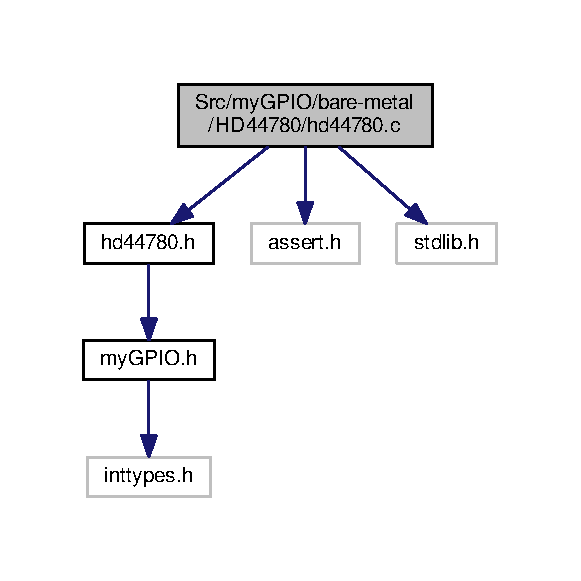
\includegraphics[width=279pt]{hd44780_8c__incl}
\end{center}
\end{figure}
\subsection*{Definizioni}
\begin{DoxyCompactItemize}
\item 
\#define \hyperlink{hd44780_8c_abc1164ac56b1a748e0ad8319be7dede8}{H\+D44780\+\_\+clear}~0x01
\item 
\#define \hyperlink{hd44780_8c_a04358db2424f9713cfb84a4fdef5b215}{H\+D44780\+\_\+home}~0x02
\item 
\#define \hyperlink{hd44780_8c_ab2681dc65568d9ec0818989aafe2eceb}{H\+D44780\+\_\+row1}~0x80
\item 
\#define \hyperlink{hd44780_8c_a7d9675a9d89c1228ada73be6239f7ef6}{H\+D44780\+\_\+row2}~0x\+C0
\item 
\#define \hyperlink{hd44780_8c_a3e52e42643f6840db3e878e23a3f82d9}{H\+D44780\+\_\+cursor\+\_\+r}~0x14
\item 
\#define \hyperlink{hd44780_8c_ad599eadde9b68b5c84f26575229383cc}{H\+D44780\+\_\+cursor\+\_\+l}~0x10
\item 
\#define \hyperlink{hd44780_8c_ab74128cead7d82100cff55cac513457a}{H\+D44780\+\_\+display\+\_\+off}~0x08
\item 
\#define \hyperlink{hd44780_8c_a05c02e143086d4d3e16c651da46357e5}{H\+D44780\+\_\+cursor\+\_\+off}~0x0\+C
\item 
\#define \hyperlink{hd44780_8c_a3967b259a0236cb4ff71b58e9e99d871}{H\+D44780\+\_\+cursor\+\_\+on}~0x0\+E
\item 
\#define \hyperlink{hd44780_8c_aee7a3931ecea03871d152b6f2fe237de}{H\+D44780\+\_\+cursor\+\_\+blink}~0x0\+F
\item 
\#define \hyperlink{hd44780_8c_abc1164ac56b1a748e0ad8319be7dede8}{H\+D44780\+\_\+clear}~0x01
\item 
\#define \hyperlink{hd44780_8c_a89582792c79342e5e196c3af6b58e813}{H\+D44780\+\_\+dec\+\_\+no\+\_\+shift}~0x04
\item 
\#define \hyperlink{hd44780_8c_a46be67bdaf1d9806e6080fc8a302e9f4}{H\+D44780\+\_\+dec\+\_\+shift}~0x05
\item 
\#define \hyperlink{hd44780_8c_a7998cf2572859cfc7a96146f9d84a8e6}{H\+D44780\+\_\+inc\+\_\+no\+\_\+shift}~0x06
\item 
\#define \hyperlink{hd44780_8c_a6c116ccd854428b9977ace77603e98f9}{H\+D44780\+\_\+inc\+\_\+shift}~0x07
\item 
\#define \hyperlink{hd44780_8c_a5f45c877d1e8266f8a2c1d0b87746950}{timer\+\_\+wait\+\_\+ms}(ms)~usleep(ms$<$$<$10)
\item 
\#define \hyperlink{hd44780_8c_a9f0a484de0de3ab1ddd77d5f716dea96}{timer\+\_\+wait\+\_\+us}(us)~usleep(us)
\item 
\#define \hyperlink{hd44780_8c_a5060e38ac985451fad57ed890aea1d77}{lcd\+\_\+command}(lcd)~\hyperlink{group__my_g_p_i_o_gab742e68093ad4c90fe299b64fd6736ca}{my\+G\+P\+I\+O\+\_\+set\+Value}(lcd-\/$>$gpio, lcd-\/$>$R\+S, \hyperlink{group__my_g_p_i_o_ggaf634fe4a0e1eab8da5000b72d6ad362ba98cde80dbda025bd1ae7231c76b55674}{my\+G\+P\+I\+O\+\_\+reset})
\item 
\#define \hyperlink{hd44780_8c_afac15d58a1ee77e8a17bc57252468ea1}{lcd\+\_\+data}(lcd)~\hyperlink{group__my_g_p_i_o_gab742e68093ad4c90fe299b64fd6736ca}{my\+G\+P\+I\+O\+\_\+set\+Value}(lcd-\/$>$gpio, lcd-\/$>$R\+S, \hyperlink{group__my_g_p_i_o_ggaf634fe4a0e1eab8da5000b72d6ad362ba10d296f3711d01189cc6c2d87f7c9149}{my\+G\+P\+I\+O\+\_\+set})
\item 
\#define \hyperlink{hd44780_8c_a7546bbb2f97e50a0469cf71934ac18e2}{lcd\+\_\+write}(lcd)~\hyperlink{group__my_g_p_i_o_gab742e68093ad4c90fe299b64fd6736ca}{my\+G\+P\+I\+O\+\_\+set\+Value}(lcd-\/$>$gpio, lcd-\/$>$R\+W, \hyperlink{group__my_g_p_i_o_ggaf634fe4a0e1eab8da5000b72d6ad362ba98cde80dbda025bd1ae7231c76b55674}{my\+G\+P\+I\+O\+\_\+reset})
\item 
\#define \hyperlink{hd44780_8c_ad7be3fdeebf9b76a774a6c1afa7fa3c8}{lcd\+\_\+read}(lcd)~\hyperlink{group__my_g_p_i_o_gab742e68093ad4c90fe299b64fd6736ca}{my\+G\+P\+I\+O\+\_\+set\+Value}(lcd-\/$>$gpio, lcd-\/$>$R\+W, \hyperlink{group__my_g_p_i_o_ggaf634fe4a0e1eab8da5000b72d6ad362ba10d296f3711d01189cc6c2d87f7c9149}{my\+G\+P\+I\+O\+\_\+set})
\item 
\#define \hyperlink{hd44780_8c_acd814f8ff18cac325b1f9f5957dd3846}{lcd\+\_\+enable}(lcd)
\end{DoxyCompactItemize}
\subsection*{Funzioni}
\begin{DoxyCompactItemize}
\item 
void \hyperlink{hd44780_8c_acc20a0564ce460f33fc998f18dd9f345}{H\+D44780\+\_\+\+Set\+Byte} (\hyperlink{struct_h_d44780___l_c_d__t}{H\+D44780\+\_\+\+L\+C\+D\+\_\+t} $\ast$lcd, uint8\+\_\+t byte)
\item 
void \hyperlink{hd44780_8c_ae12ebf4e3dd52b7d10f155e0dd1b4898}{H\+D44780\+\_\+\+Write\+Command} (\hyperlink{struct_h_d44780___l_c_d__t}{H\+D44780\+\_\+\+L\+C\+D\+\_\+t} $\ast$lcd, uint8\+\_\+t command)
\item 
void \hyperlink{hd44780_8c_a39e7e22ae76f1eec9aaf0933af398f4b}{H\+D44780\+\_\+\+Write\+Data} (\hyperlink{struct_h_d44780___l_c_d__t}{H\+D44780\+\_\+\+L\+C\+D\+\_\+t} $\ast$lcd, uint8\+\_\+t data)
\item 
int \hyperlink{hd44780_8c_ad3c60edaac713488ecb9c7ed73854a3c}{H\+D44780\+\_\+\+Validate\+Pair} (\hyperlink{struct_h_d44780___l_c_d__t}{H\+D44780\+\_\+\+L\+C\+D\+\_\+t} $\ast$lcd)
\item 
void \hyperlink{hd44780_8c_ad4120d3a2df038c193d043f386fdb221}{H\+D44780\+\_\+\+Configure\+Pin} (\hyperlink{struct_h_d44780___l_c_d__t}{H\+D44780\+\_\+\+L\+C\+D\+\_\+t} $\ast$lcd)
\item 
void \hyperlink{group___h_d44780_gad212907e20316f4fc0e93d7c7a8f338e}{H\+D44780\+\_\+\+Init8} (\hyperlink{struct_h_d44780___l_c_d__t}{H\+D44780\+\_\+\+L\+C\+D\+\_\+t} $\ast$lcd, \hyperlink{structmy_g_p_i_o__t}{my\+G\+P\+I\+O\+\_\+t} $\ast$gpio, \hyperlink{group__my_g_p_i_o_ga402a0d20afc0cb7c25554b8b023f4253}{my\+G\+P\+I\+O\+\_\+mask} R\+S, \hyperlink{group__my_g_p_i_o_ga402a0d20afc0cb7c25554b8b023f4253}{my\+G\+P\+I\+O\+\_\+mask} R\+W, \hyperlink{group__my_g_p_i_o_ga402a0d20afc0cb7c25554b8b023f4253}{my\+G\+P\+I\+O\+\_\+mask} E, \hyperlink{group__my_g_p_i_o_ga402a0d20afc0cb7c25554b8b023f4253}{my\+G\+P\+I\+O\+\_\+mask} Data7, \hyperlink{group__my_g_p_i_o_ga402a0d20afc0cb7c25554b8b023f4253}{my\+G\+P\+I\+O\+\_\+mask} Data6, \hyperlink{group__my_g_p_i_o_ga402a0d20afc0cb7c25554b8b023f4253}{my\+G\+P\+I\+O\+\_\+mask} Data5, \hyperlink{group__my_g_p_i_o_ga402a0d20afc0cb7c25554b8b023f4253}{my\+G\+P\+I\+O\+\_\+mask} Data4, \hyperlink{group__my_g_p_i_o_ga402a0d20afc0cb7c25554b8b023f4253}{my\+G\+P\+I\+O\+\_\+mask} Data3, \hyperlink{group__my_g_p_i_o_ga402a0d20afc0cb7c25554b8b023f4253}{my\+G\+P\+I\+O\+\_\+mask} Data2, \hyperlink{group__my_g_p_i_o_ga402a0d20afc0cb7c25554b8b023f4253}{my\+G\+P\+I\+O\+\_\+mask} Data1, \hyperlink{group__my_g_p_i_o_ga402a0d20afc0cb7c25554b8b023f4253}{my\+G\+P\+I\+O\+\_\+mask} Data0)
\begin{DoxyCompactList}\small\item\em Inizializza un display lcd H\+D44780 con interfacciamento ad 8 bit. \end{DoxyCompactList}\item 
void \hyperlink{group___h_d44780_ga0c08f9e41d770ebfa4af385a56b47b81}{H\+D44780\+\_\+\+Init4} (\hyperlink{struct_h_d44780___l_c_d__t}{H\+D44780\+\_\+\+L\+C\+D\+\_\+t} $\ast$lcd, \hyperlink{structmy_g_p_i_o__t}{my\+G\+P\+I\+O\+\_\+t} $\ast$gpio, \hyperlink{group__my_g_p_i_o_ga402a0d20afc0cb7c25554b8b023f4253}{my\+G\+P\+I\+O\+\_\+mask} R\+S, \hyperlink{group__my_g_p_i_o_ga402a0d20afc0cb7c25554b8b023f4253}{my\+G\+P\+I\+O\+\_\+mask} R\+W, \hyperlink{group__my_g_p_i_o_ga402a0d20afc0cb7c25554b8b023f4253}{my\+G\+P\+I\+O\+\_\+mask} E, \hyperlink{group__my_g_p_i_o_ga402a0d20afc0cb7c25554b8b023f4253}{my\+G\+P\+I\+O\+\_\+mask} Data7, \hyperlink{group__my_g_p_i_o_ga402a0d20afc0cb7c25554b8b023f4253}{my\+G\+P\+I\+O\+\_\+mask} Data6, \hyperlink{group__my_g_p_i_o_ga402a0d20afc0cb7c25554b8b023f4253}{my\+G\+P\+I\+O\+\_\+mask} Data5, \hyperlink{group__my_g_p_i_o_ga402a0d20afc0cb7c25554b8b023f4253}{my\+G\+P\+I\+O\+\_\+mask} Data4)
\begin{DoxyCompactList}\small\item\em Inizializza un oggetto display lcd H\+D44780 affinche' si utilizzi l'interfaccia a 4 bit. \end{DoxyCompactList}\item 
void \hyperlink{group___h_d44780_ga57b8c6ca0b3c12e5f7273b3c373a6f17}{H\+D44780\+\_\+\+Printc} (\hyperlink{struct_h_d44780___l_c_d__t}{H\+D44780\+\_\+\+L\+C\+D\+\_\+t} $\ast$lcd, char c)
\begin{DoxyCompactList}\small\item\em Stampa un carattere. \end{DoxyCompactList}\item 
void \hyperlink{group___h_d44780_ga3aedff8e2040e62db569fde955d3987b}{H\+D44780\+\_\+\+Print} (\hyperlink{struct_h_d44780___l_c_d__t}{H\+D44780\+\_\+\+L\+C\+D\+\_\+t} $\ast$lcd, const char $\ast$s)
\begin{DoxyCompactList}\small\item\em Stampa una stringa null-\/terminated di caratteri. \end{DoxyCompactList}\item 
void \hyperlink{group___h_d44780_ga2a5d4d528175321c46c790b581959e63}{H\+D44780\+\_\+print\+Binary8} (\hyperlink{struct_h_d44780___l_c_d__t}{H\+D44780\+\_\+\+L\+C\+D\+\_\+t} $\ast$lcd, uint8\+\_\+t b)
\begin{DoxyCompactList}\small\item\em Stampa un byte in binario. (bit piu' significativo a sinistra) \end{DoxyCompactList}\item 
void \hyperlink{group___h_d44780_ga95cceef2401c5519295e5a83c6688b5c}{H\+D44780\+\_\+print\+Binary32} (\hyperlink{struct_h_d44780___l_c_d__t}{H\+D44780\+\_\+\+L\+C\+D\+\_\+t} $\ast$lcd, uint32\+\_\+t w)
\begin{DoxyCompactList}\small\item\em Stampa una word di 32 bit in binario. (bit piu' significativo a sinistra) \end{DoxyCompactList}\item 
void \hyperlink{group___h_d44780_ga0f99bc5458acb172d0f3bfeb94f90e2a}{H\+D44780\+\_\+print\+Binary64} (\hyperlink{struct_h_d44780___l_c_d__t}{H\+D44780\+\_\+\+L\+C\+D\+\_\+t} $\ast$lcd, uint64\+\_\+t b)
\begin{DoxyCompactList}\small\item\em Stampa un blocco di 64 bit in binario. (bit piu' significativo a sinistra) \end{DoxyCompactList}\item 
void \hyperlink{group___h_d44780_gad967bd458b4d2bd358a93cbb7144addd}{H\+D44780\+\_\+print\+Hex8} (\hyperlink{struct_h_d44780___l_c_d__t}{H\+D44780\+\_\+\+L\+C\+D\+\_\+t} $\ast$lcd, uint8\+\_\+t b)
\begin{DoxyCompactList}\small\item\em Stampa un byte in esadecimale. (bit piu' significativo a sinistra) \end{DoxyCompactList}\item 
void \hyperlink{group___h_d44780_gaa82a2a27a3008f55c969a2d390c50497}{H\+D44780\+\_\+print\+Hex32} (\hyperlink{struct_h_d44780___l_c_d__t}{H\+D44780\+\_\+\+L\+C\+D\+\_\+t} $\ast$lcd, uint32\+\_\+t w)
\begin{DoxyCompactList}\small\item\em Stampa una word di 32 bit in esadecimale. (bit piu' significativo a sinistra) \end{DoxyCompactList}\item 
void \hyperlink{group___h_d44780_ga7a4b110e7da806f8c01e01d184d3a19a}{H\+D44780\+\_\+print\+Hex64} (\hyperlink{struct_h_d44780___l_c_d__t}{H\+D44780\+\_\+\+L\+C\+D\+\_\+t} $\ast$lcd, uint64\+\_\+t b)
\begin{DoxyCompactList}\small\item\em Stampa un blocco di 64 bit in esadecimale. (bit piu' significativo a sinistra) \end{DoxyCompactList}\item 
void \hyperlink{group___h_d44780_ga38cac13d7a66f068be54f79a716ff7d4}{H\+D44780\+\_\+\+Clear} (\hyperlink{struct_h_d44780___l_c_d__t}{H\+D44780\+\_\+\+L\+C\+D\+\_\+t} $\ast$lcd)
\begin{DoxyCompactList}\small\item\em Pulisce il display e sposta il cursore all'inizio della prima riga. \end{DoxyCompactList}\item 
void \hyperlink{group___h_d44780_ga68e3712332aa9482d4bdaa4991a92127}{H\+D44780\+\_\+\+Home} (\hyperlink{struct_h_d44780___l_c_d__t}{H\+D44780\+\_\+\+L\+C\+D\+\_\+t} $\ast$lcd)
\begin{DoxyCompactList}\small\item\em Sposta il cursore all'inizio della prima riga. \end{DoxyCompactList}\item 
void \hyperlink{group___h_d44780_gad90e2924a4e632ce42940323f8f49e37}{H\+D44780\+\_\+\+Move\+To\+Row1} (\hyperlink{struct_h_d44780___l_c_d__t}{H\+D44780\+\_\+\+L\+C\+D\+\_\+t} $\ast$lcd)
\begin{DoxyCompactList}\small\item\em Sposta il cursore all'inizio della prima riga. \end{DoxyCompactList}\item 
void \hyperlink{group___h_d44780_ga713670d498b6f5d50a174df19081c515}{H\+D44780\+\_\+\+Move\+To\+Row2} (\hyperlink{struct_h_d44780___l_c_d__t}{H\+D44780\+\_\+\+L\+C\+D\+\_\+t} $\ast$lcd)
\begin{DoxyCompactList}\small\item\em Sposta il cursore all'inizio della seconda riga. \end{DoxyCompactList}\item 
void \hyperlink{group___h_d44780_gabcea9a03050c46530e39b7556c673baf}{H\+D44780\+\_\+\+Move\+Cursor} (\hyperlink{struct_h_d44780___l_c_d__t}{H\+D44780\+\_\+\+L\+C\+D\+\_\+t} $\ast$lcd, \hyperlink{group___h_d44780_gaf46f4db4f981d3a1088804a6d6980d30}{H\+D44780\+\_\+\+Direction\+\_\+t} dir)
\begin{DoxyCompactList}\small\item\em Sposta il cursore di una posizione a destra o sinistra. \end{DoxyCompactList}\item 
void \hyperlink{group___h_d44780_ga5cf07b2179272029410f9a81f56621ed}{H\+D44780\+\_\+\+Display\+Off} (\hyperlink{struct_h_d44780___l_c_d__t}{H\+D44780\+\_\+\+L\+C\+D\+\_\+t} $\ast$lcd)
\begin{DoxyCompactList}\small\item\em Disattiva il display. \end{DoxyCompactList}\item 
void \hyperlink{group___h_d44780_ga56421dc398825188aa10257063a3ee4b}{H\+D44780\+\_\+\+Cursor\+Off} (\hyperlink{struct_h_d44780___l_c_d__t}{H\+D44780\+\_\+\+L\+C\+D\+\_\+t} $\ast$lcd)
\begin{DoxyCompactList}\small\item\em Disattiva la visualizzazione del cursore. \end{DoxyCompactList}\item 
void \hyperlink{group___h_d44780_ga3a381cb44df5d76d79be5ed71a52bae6}{H\+D44780\+\_\+\+Cursor\+On} (\hyperlink{struct_h_d44780___l_c_d__t}{H\+D44780\+\_\+\+L\+C\+D\+\_\+t} $\ast$lcd)
\begin{DoxyCompactList}\small\item\em Attiva la visualizzazione del cursore. \end{DoxyCompactList}\item 
void \hyperlink{group___h_d44780_ga92eb58cb7d73c9a87b7087a9c56f73d5}{H\+D44780\+\_\+\+Cursor\+Blink} (\hyperlink{struct_h_d44780___l_c_d__t}{H\+D44780\+\_\+\+L\+C\+D\+\_\+t} $\ast$lcd)
\begin{DoxyCompactList}\small\item\em Attiva il cursore lampeggiante. \end{DoxyCompactList}\end{DoxyCompactItemize}


\subsection{Descrizione dettagliata}
\begin{DoxyAuthor}{Autore}
Salvatore Barone \href{mailto:salvator.barone@gmail.com}{\tt salvator.\+barone@gmail.\+com}
\end{DoxyAuthor}
\begin{DoxyCopyright}{Copyright}
Copyright 2017 Salvatore Barone \href{mailto:salvator.barone@gmail.com}{\tt salvator.\+barone@gmail.\+com}
\end{DoxyCopyright}
This file is part of Zynq7000\+Driver\+Pack

Zynq7000\+Driver\+Pack is free software; you can redistribute it and/or modify it under the terms of the G\+N\+U General Public License as published by the Free Software Foundation; either version 3 of the License, or any later version.

Zynq7000\+Driver\+Pack is distributed in the hope that it will be useful, but W\+I\+T\+H\+O\+U\+T A\+N\+Y W\+A\+R\+R\+A\+N\+T\+Y; without even the implied warranty of M\+E\+R\+C\+H\+A\+N\+T\+A\+B\+I\+L\+I\+T\+Y or F\+I\+T\+N\+E\+S\+S F\+O\+R A P\+A\+R\+T\+I\+C\+U\+L\+A\+R P\+U\+R\+P\+O\+S\+E. See the G\+N\+U General Public License for more details.

You should have received a copy of the G\+N\+U General Public License along with this program; if not, write to the Free Software Foundation, Inc., 51 Franklin Street, Fifth Floor, Boston, M\+A 02110-\/1301, U\+S\+A. 

\subsection{Documentazione delle definizioni}
\hypertarget{hd44780_8c_abc1164ac56b1a748e0ad8319be7dede8}{\index{hd44780.\+c@{hd44780.\+c}!H\+D44780\+\_\+clear@{H\+D44780\+\_\+clear}}
\index{H\+D44780\+\_\+clear@{H\+D44780\+\_\+clear}!hd44780.\+c@{hd44780.\+c}}
\subsubsection[{H\+D44780\+\_\+clear}]{\setlength{\rightskip}{0pt plus 5cm}\#define H\+D44780\+\_\+clear~0x01}}\label{hd44780_8c_abc1164ac56b1a748e0ad8319be7dede8}
\hypertarget{hd44780_8c_abc1164ac56b1a748e0ad8319be7dede8}{\index{hd44780.\+c@{hd44780.\+c}!H\+D44780\+\_\+clear@{H\+D44780\+\_\+clear}}
\index{H\+D44780\+\_\+clear@{H\+D44780\+\_\+clear}!hd44780.\+c@{hd44780.\+c}}
\subsubsection[{H\+D44780\+\_\+clear}]{\setlength{\rightskip}{0pt plus 5cm}\#define H\+D44780\+\_\+clear~0x01}}\label{hd44780_8c_abc1164ac56b1a748e0ad8319be7dede8}
\hypertarget{hd44780_8c_aee7a3931ecea03871d152b6f2fe237de}{\index{hd44780.\+c@{hd44780.\+c}!H\+D44780\+\_\+cursor\+\_\+blink@{H\+D44780\+\_\+cursor\+\_\+blink}}
\index{H\+D44780\+\_\+cursor\+\_\+blink@{H\+D44780\+\_\+cursor\+\_\+blink}!hd44780.\+c@{hd44780.\+c}}
\subsubsection[{H\+D44780\+\_\+cursor\+\_\+blink}]{\setlength{\rightskip}{0pt plus 5cm}\#define H\+D44780\+\_\+cursor\+\_\+blink~0x0\+F}}\label{hd44780_8c_aee7a3931ecea03871d152b6f2fe237de}
\hypertarget{hd44780_8c_ad599eadde9b68b5c84f26575229383cc}{\index{hd44780.\+c@{hd44780.\+c}!H\+D44780\+\_\+cursor\+\_\+l@{H\+D44780\+\_\+cursor\+\_\+l}}
\index{H\+D44780\+\_\+cursor\+\_\+l@{H\+D44780\+\_\+cursor\+\_\+l}!hd44780.\+c@{hd44780.\+c}}
\subsubsection[{H\+D44780\+\_\+cursor\+\_\+l}]{\setlength{\rightskip}{0pt plus 5cm}\#define H\+D44780\+\_\+cursor\+\_\+l~0x10}}\label{hd44780_8c_ad599eadde9b68b5c84f26575229383cc}
\hypertarget{hd44780_8c_a05c02e143086d4d3e16c651da46357e5}{\index{hd44780.\+c@{hd44780.\+c}!H\+D44780\+\_\+cursor\+\_\+off@{H\+D44780\+\_\+cursor\+\_\+off}}
\index{H\+D44780\+\_\+cursor\+\_\+off@{H\+D44780\+\_\+cursor\+\_\+off}!hd44780.\+c@{hd44780.\+c}}
\subsubsection[{H\+D44780\+\_\+cursor\+\_\+off}]{\setlength{\rightskip}{0pt plus 5cm}\#define H\+D44780\+\_\+cursor\+\_\+off~0x0\+C}}\label{hd44780_8c_a05c02e143086d4d3e16c651da46357e5}
\hypertarget{hd44780_8c_a3967b259a0236cb4ff71b58e9e99d871}{\index{hd44780.\+c@{hd44780.\+c}!H\+D44780\+\_\+cursor\+\_\+on@{H\+D44780\+\_\+cursor\+\_\+on}}
\index{H\+D44780\+\_\+cursor\+\_\+on@{H\+D44780\+\_\+cursor\+\_\+on}!hd44780.\+c@{hd44780.\+c}}
\subsubsection[{H\+D44780\+\_\+cursor\+\_\+on}]{\setlength{\rightskip}{0pt plus 5cm}\#define H\+D44780\+\_\+cursor\+\_\+on~0x0\+E}}\label{hd44780_8c_a3967b259a0236cb4ff71b58e9e99d871}
\hypertarget{hd44780_8c_a3e52e42643f6840db3e878e23a3f82d9}{\index{hd44780.\+c@{hd44780.\+c}!H\+D44780\+\_\+cursor\+\_\+r@{H\+D44780\+\_\+cursor\+\_\+r}}
\index{H\+D44780\+\_\+cursor\+\_\+r@{H\+D44780\+\_\+cursor\+\_\+r}!hd44780.\+c@{hd44780.\+c}}
\subsubsection[{H\+D44780\+\_\+cursor\+\_\+r}]{\setlength{\rightskip}{0pt plus 5cm}\#define H\+D44780\+\_\+cursor\+\_\+r~0x14}}\label{hd44780_8c_a3e52e42643f6840db3e878e23a3f82d9}
\hypertarget{hd44780_8c_a89582792c79342e5e196c3af6b58e813}{\index{hd44780.\+c@{hd44780.\+c}!H\+D44780\+\_\+dec\+\_\+no\+\_\+shift@{H\+D44780\+\_\+dec\+\_\+no\+\_\+shift}}
\index{H\+D44780\+\_\+dec\+\_\+no\+\_\+shift@{H\+D44780\+\_\+dec\+\_\+no\+\_\+shift}!hd44780.\+c@{hd44780.\+c}}
\subsubsection[{H\+D44780\+\_\+dec\+\_\+no\+\_\+shift}]{\setlength{\rightskip}{0pt plus 5cm}\#define H\+D44780\+\_\+dec\+\_\+no\+\_\+shift~0x04}}\label{hd44780_8c_a89582792c79342e5e196c3af6b58e813}
\hypertarget{hd44780_8c_a46be67bdaf1d9806e6080fc8a302e9f4}{\index{hd44780.\+c@{hd44780.\+c}!H\+D44780\+\_\+dec\+\_\+shift@{H\+D44780\+\_\+dec\+\_\+shift}}
\index{H\+D44780\+\_\+dec\+\_\+shift@{H\+D44780\+\_\+dec\+\_\+shift}!hd44780.\+c@{hd44780.\+c}}
\subsubsection[{H\+D44780\+\_\+dec\+\_\+shift}]{\setlength{\rightskip}{0pt plus 5cm}\#define H\+D44780\+\_\+dec\+\_\+shift~0x05}}\label{hd44780_8c_a46be67bdaf1d9806e6080fc8a302e9f4}
\hypertarget{hd44780_8c_ab74128cead7d82100cff55cac513457a}{\index{hd44780.\+c@{hd44780.\+c}!H\+D44780\+\_\+display\+\_\+off@{H\+D44780\+\_\+display\+\_\+off}}
\index{H\+D44780\+\_\+display\+\_\+off@{H\+D44780\+\_\+display\+\_\+off}!hd44780.\+c@{hd44780.\+c}}
\subsubsection[{H\+D44780\+\_\+display\+\_\+off}]{\setlength{\rightskip}{0pt plus 5cm}\#define H\+D44780\+\_\+display\+\_\+off~0x08}}\label{hd44780_8c_ab74128cead7d82100cff55cac513457a}
\hypertarget{hd44780_8c_a04358db2424f9713cfb84a4fdef5b215}{\index{hd44780.\+c@{hd44780.\+c}!H\+D44780\+\_\+home@{H\+D44780\+\_\+home}}
\index{H\+D44780\+\_\+home@{H\+D44780\+\_\+home}!hd44780.\+c@{hd44780.\+c}}
\subsubsection[{H\+D44780\+\_\+home}]{\setlength{\rightskip}{0pt plus 5cm}\#define H\+D44780\+\_\+home~0x02}}\label{hd44780_8c_a04358db2424f9713cfb84a4fdef5b215}
\hypertarget{hd44780_8c_a7998cf2572859cfc7a96146f9d84a8e6}{\index{hd44780.\+c@{hd44780.\+c}!H\+D44780\+\_\+inc\+\_\+no\+\_\+shift@{H\+D44780\+\_\+inc\+\_\+no\+\_\+shift}}
\index{H\+D44780\+\_\+inc\+\_\+no\+\_\+shift@{H\+D44780\+\_\+inc\+\_\+no\+\_\+shift}!hd44780.\+c@{hd44780.\+c}}
\subsubsection[{H\+D44780\+\_\+inc\+\_\+no\+\_\+shift}]{\setlength{\rightskip}{0pt plus 5cm}\#define H\+D44780\+\_\+inc\+\_\+no\+\_\+shift~0x06}}\label{hd44780_8c_a7998cf2572859cfc7a96146f9d84a8e6}
\hypertarget{hd44780_8c_a6c116ccd854428b9977ace77603e98f9}{\index{hd44780.\+c@{hd44780.\+c}!H\+D44780\+\_\+inc\+\_\+shift@{H\+D44780\+\_\+inc\+\_\+shift}}
\index{H\+D44780\+\_\+inc\+\_\+shift@{H\+D44780\+\_\+inc\+\_\+shift}!hd44780.\+c@{hd44780.\+c}}
\subsubsection[{H\+D44780\+\_\+inc\+\_\+shift}]{\setlength{\rightskip}{0pt plus 5cm}\#define H\+D44780\+\_\+inc\+\_\+shift~0x07}}\label{hd44780_8c_a6c116ccd854428b9977ace77603e98f9}
\hypertarget{hd44780_8c_ab2681dc65568d9ec0818989aafe2eceb}{\index{hd44780.\+c@{hd44780.\+c}!H\+D44780\+\_\+row1@{H\+D44780\+\_\+row1}}
\index{H\+D44780\+\_\+row1@{H\+D44780\+\_\+row1}!hd44780.\+c@{hd44780.\+c}}
\subsubsection[{H\+D44780\+\_\+row1}]{\setlength{\rightskip}{0pt plus 5cm}\#define H\+D44780\+\_\+row1~0x80}}\label{hd44780_8c_ab2681dc65568d9ec0818989aafe2eceb}
\hypertarget{hd44780_8c_a7d9675a9d89c1228ada73be6239f7ef6}{\index{hd44780.\+c@{hd44780.\+c}!H\+D44780\+\_\+row2@{H\+D44780\+\_\+row2}}
\index{H\+D44780\+\_\+row2@{H\+D44780\+\_\+row2}!hd44780.\+c@{hd44780.\+c}}
\subsubsection[{H\+D44780\+\_\+row2}]{\setlength{\rightskip}{0pt plus 5cm}\#define H\+D44780\+\_\+row2~0x\+C0}}\label{hd44780_8c_a7d9675a9d89c1228ada73be6239f7ef6}
\hypertarget{hd44780_8c_a5060e38ac985451fad57ed890aea1d77}{\index{hd44780.\+c@{hd44780.\+c}!lcd\+\_\+command@{lcd\+\_\+command}}
\index{lcd\+\_\+command@{lcd\+\_\+command}!hd44780.\+c@{hd44780.\+c}}
\subsubsection[{lcd\+\_\+command}]{\setlength{\rightskip}{0pt plus 5cm}\#define lcd\+\_\+command(
\begin{DoxyParamCaption}
\item[{}]{lcd}
\end{DoxyParamCaption}
)~{\bf my\+G\+P\+I\+O\+\_\+set\+Value}(lcd-\/$>$gpio, lcd-\/$>$R\+S, {\bf my\+G\+P\+I\+O\+\_\+reset})}}\label{hd44780_8c_a5060e38ac985451fad57ed890aea1d77}
\hypertarget{hd44780_8c_afac15d58a1ee77e8a17bc57252468ea1}{\index{hd44780.\+c@{hd44780.\+c}!lcd\+\_\+data@{lcd\+\_\+data}}
\index{lcd\+\_\+data@{lcd\+\_\+data}!hd44780.\+c@{hd44780.\+c}}
\subsubsection[{lcd\+\_\+data}]{\setlength{\rightskip}{0pt plus 5cm}\#define lcd\+\_\+data(
\begin{DoxyParamCaption}
\item[{}]{lcd}
\end{DoxyParamCaption}
)~{\bf my\+G\+P\+I\+O\+\_\+set\+Value}(lcd-\/$>$gpio, lcd-\/$>$R\+S, {\bf my\+G\+P\+I\+O\+\_\+set})}}\label{hd44780_8c_afac15d58a1ee77e8a17bc57252468ea1}
\hypertarget{hd44780_8c_acd814f8ff18cac325b1f9f5957dd3846}{\index{hd44780.\+c@{hd44780.\+c}!lcd\+\_\+enable@{lcd\+\_\+enable}}
\index{lcd\+\_\+enable@{lcd\+\_\+enable}!hd44780.\+c@{hd44780.\+c}}
\subsubsection[{lcd\+\_\+enable}]{\setlength{\rightskip}{0pt plus 5cm}\#define lcd\+\_\+enable(
\begin{DoxyParamCaption}
\item[{}]{lcd}
\end{DoxyParamCaption}
)}}\label{hd44780_8c_acd814f8ff18cac325b1f9f5957dd3846}
{\bfseries Valore\+:}
\begin{DoxyCode}
\hyperlink{group__my_g_p_i_o_gab742e68093ad4c90fe299b64fd6736ca}{myGPIO\_setValue}(lcd->gpio, lcd->E, \hyperlink{group__my_g_p_i_o_ggaf634fe4a0e1eab8da5000b72d6ad362ba10d296f3711d01189cc6c2d87f7c9149}{myGPIO\_set}); \hyperlink{hd44780_8c_a9f0a484de0de3ab1ddd77d5f716dea96}{\(\backslash\)}
\hyperlink{hd44780_8c_a9f0a484de0de3ab1ddd77d5f716dea96}{                            timer\_wait\_us}(100); \hyperlink{group__my_g_p_i_o_gab742e68093ad4c90fe299b64fd6736ca}{\(\backslash\)}
\hyperlink{group__my_g_p_i_o_gab742e68093ad4c90fe299b64fd6736ca}{                            myGPIO\_setValue}(lcd->gpio, lcd->E, 
      \hyperlink{group__my_g_p_i_o_ggaf634fe4a0e1eab8da5000b72d6ad362ba98cde80dbda025bd1ae7231c76b55674}{myGPIO\_reset})
\end{DoxyCode}
\hypertarget{hd44780_8c_ad7be3fdeebf9b76a774a6c1afa7fa3c8}{\index{hd44780.\+c@{hd44780.\+c}!lcd\+\_\+read@{lcd\+\_\+read}}
\index{lcd\+\_\+read@{lcd\+\_\+read}!hd44780.\+c@{hd44780.\+c}}
\subsubsection[{lcd\+\_\+read}]{\setlength{\rightskip}{0pt plus 5cm}\#define lcd\+\_\+read(
\begin{DoxyParamCaption}
\item[{}]{lcd}
\end{DoxyParamCaption}
)~{\bf my\+G\+P\+I\+O\+\_\+set\+Value}(lcd-\/$>$gpio, lcd-\/$>$R\+W, {\bf my\+G\+P\+I\+O\+\_\+set})}}\label{hd44780_8c_ad7be3fdeebf9b76a774a6c1afa7fa3c8}
\hypertarget{hd44780_8c_a7546bbb2f97e50a0469cf71934ac18e2}{\index{hd44780.\+c@{hd44780.\+c}!lcd\+\_\+write@{lcd\+\_\+write}}
\index{lcd\+\_\+write@{lcd\+\_\+write}!hd44780.\+c@{hd44780.\+c}}
\subsubsection[{lcd\+\_\+write}]{\setlength{\rightskip}{0pt plus 5cm}\#define lcd\+\_\+write(
\begin{DoxyParamCaption}
\item[{}]{lcd}
\end{DoxyParamCaption}
)~{\bf my\+G\+P\+I\+O\+\_\+set\+Value}(lcd-\/$>$gpio, lcd-\/$>$R\+W, {\bf my\+G\+P\+I\+O\+\_\+reset})}}\label{hd44780_8c_a7546bbb2f97e50a0469cf71934ac18e2}
\hypertarget{hd44780_8c_a5f45c877d1e8266f8a2c1d0b87746950}{\index{hd44780.\+c@{hd44780.\+c}!timer\+\_\+wait\+\_\+ms@{timer\+\_\+wait\+\_\+ms}}
\index{timer\+\_\+wait\+\_\+ms@{timer\+\_\+wait\+\_\+ms}!hd44780.\+c@{hd44780.\+c}}
\subsubsection[{timer\+\_\+wait\+\_\+ms}]{\setlength{\rightskip}{0pt plus 5cm}\#define timer\+\_\+wait\+\_\+ms(
\begin{DoxyParamCaption}
\item[{}]{ms}
\end{DoxyParamCaption}
)~usleep(ms$<$$<$10)}}\label{hd44780_8c_a5f45c877d1e8266f8a2c1d0b87746950}
\hypertarget{hd44780_8c_a9f0a484de0de3ab1ddd77d5f716dea96}{\index{hd44780.\+c@{hd44780.\+c}!timer\+\_\+wait\+\_\+us@{timer\+\_\+wait\+\_\+us}}
\index{timer\+\_\+wait\+\_\+us@{timer\+\_\+wait\+\_\+us}!hd44780.\+c@{hd44780.\+c}}
\subsubsection[{timer\+\_\+wait\+\_\+us}]{\setlength{\rightskip}{0pt plus 5cm}\#define timer\+\_\+wait\+\_\+us(
\begin{DoxyParamCaption}
\item[{}]{us}
\end{DoxyParamCaption}
)~usleep(us)}}\label{hd44780_8c_a9f0a484de0de3ab1ddd77d5f716dea96}


\subsection{Documentazione delle funzioni}
\hypertarget{hd44780_8c_ad4120d3a2df038c193d043f386fdb221}{\index{hd44780.\+c@{hd44780.\+c}!H\+D44780\+\_\+\+Configure\+Pin@{H\+D44780\+\_\+\+Configure\+Pin}}
\index{H\+D44780\+\_\+\+Configure\+Pin@{H\+D44780\+\_\+\+Configure\+Pin}!hd44780.\+c@{hd44780.\+c}}
\subsubsection[{H\+D44780\+\_\+\+Configure\+Pin}]{\setlength{\rightskip}{0pt plus 5cm}void H\+D44780\+\_\+\+Configure\+Pin (
\begin{DoxyParamCaption}
\item[{{\bf H\+D44780\+\_\+\+L\+C\+D\+\_\+t} $\ast$}]{lcd}
\end{DoxyParamCaption}
)}}\label{hd44780_8c_ad4120d3a2df038c193d043f386fdb221}
\hypertarget{hd44780_8c_acc20a0564ce460f33fc998f18dd9f345}{\index{hd44780.\+c@{hd44780.\+c}!H\+D44780\+\_\+\+Set\+Byte@{H\+D44780\+\_\+\+Set\+Byte}}
\index{H\+D44780\+\_\+\+Set\+Byte@{H\+D44780\+\_\+\+Set\+Byte}!hd44780.\+c@{hd44780.\+c}}
\subsubsection[{H\+D44780\+\_\+\+Set\+Byte}]{\setlength{\rightskip}{0pt plus 5cm}void H\+D44780\+\_\+\+Set\+Byte (
\begin{DoxyParamCaption}
\item[{{\bf H\+D44780\+\_\+\+L\+C\+D\+\_\+t} $\ast$}]{lcd, }
\item[{uint8\+\_\+t}]{byte}
\end{DoxyParamCaption}
)}}\label{hd44780_8c_acc20a0564ce460f33fc998f18dd9f345}
\hypertarget{hd44780_8c_ad3c60edaac713488ecb9c7ed73854a3c}{\index{hd44780.\+c@{hd44780.\+c}!H\+D44780\+\_\+\+Validate\+Pair@{H\+D44780\+\_\+\+Validate\+Pair}}
\index{H\+D44780\+\_\+\+Validate\+Pair@{H\+D44780\+\_\+\+Validate\+Pair}!hd44780.\+c@{hd44780.\+c}}
\subsubsection[{H\+D44780\+\_\+\+Validate\+Pair}]{\setlength{\rightskip}{0pt plus 5cm}int H\+D44780\+\_\+\+Validate\+Pair (
\begin{DoxyParamCaption}
\item[{{\bf H\+D44780\+\_\+\+L\+C\+D\+\_\+t} $\ast$}]{lcd}
\end{DoxyParamCaption}
)}}\label{hd44780_8c_ad3c60edaac713488ecb9c7ed73854a3c}
\hypertarget{hd44780_8c_ae12ebf4e3dd52b7d10f155e0dd1b4898}{\index{hd44780.\+c@{hd44780.\+c}!H\+D44780\+\_\+\+Write\+Command@{H\+D44780\+\_\+\+Write\+Command}}
\index{H\+D44780\+\_\+\+Write\+Command@{H\+D44780\+\_\+\+Write\+Command}!hd44780.\+c@{hd44780.\+c}}
\subsubsection[{H\+D44780\+\_\+\+Write\+Command}]{\setlength{\rightskip}{0pt plus 5cm}void H\+D44780\+\_\+\+Write\+Command (
\begin{DoxyParamCaption}
\item[{{\bf H\+D44780\+\_\+\+L\+C\+D\+\_\+t} $\ast$}]{lcd, }
\item[{uint8\+\_\+t}]{command}
\end{DoxyParamCaption}
)}}\label{hd44780_8c_ae12ebf4e3dd52b7d10f155e0dd1b4898}
\hypertarget{hd44780_8c_a39e7e22ae76f1eec9aaf0933af398f4b}{\index{hd44780.\+c@{hd44780.\+c}!H\+D44780\+\_\+\+Write\+Data@{H\+D44780\+\_\+\+Write\+Data}}
\index{H\+D44780\+\_\+\+Write\+Data@{H\+D44780\+\_\+\+Write\+Data}!hd44780.\+c@{hd44780.\+c}}
\subsubsection[{H\+D44780\+\_\+\+Write\+Data}]{\setlength{\rightskip}{0pt plus 5cm}void H\+D44780\+\_\+\+Write\+Data (
\begin{DoxyParamCaption}
\item[{{\bf H\+D44780\+\_\+\+L\+C\+D\+\_\+t} $\ast$}]{lcd, }
\item[{uint8\+\_\+t}]{data}
\end{DoxyParamCaption}
)}}\label{hd44780_8c_a39e7e22ae76f1eec9aaf0933af398f4b}

\hypertarget{hd44780_8h}{\section{Riferimenti per il file Lcd/hd44780.h}
\label{hd44780_8h}\index{Lcd/hd44780.\+h@{Lcd/hd44780.\+h}}
}
{\ttfamily \#include \char`\"{}my\+G\+P\+I\+O.\+h\char`\"{}}\\*
Grafo delle dipendenze di inclusione per hd44780.\+h\+:
\nopagebreak
\begin{figure}[H]
\begin{center}
\leavevmode
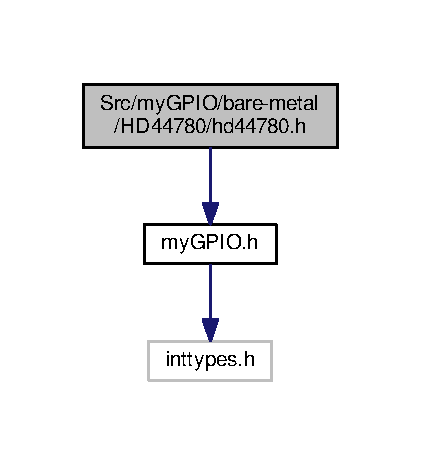
\includegraphics[width=160pt]{hd44780_8h__incl}
\end{center}
\end{figure}
Questo grafo mostra quali altri file includono direttamente o indirettamente questo file\+:\nopagebreak
\begin{figure}[H]
\begin{center}
\leavevmode
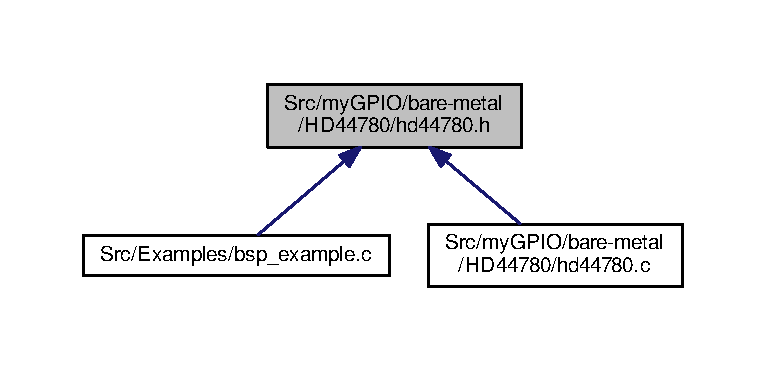
\includegraphics[width=160pt]{hd44780_8h__dep__incl}
\end{center}
\end{figure}
\subsection*{Strutture dati}
\begin{DoxyCompactItemize}
\item 
struct \hyperlink{struct_h_d44780___l_c_d__t}{H\+D44780\+\_\+\+L\+C\+D\+\_\+t}
\begin{DoxyCompactList}\small\item\em Struttura opaca che astrae un device Display L\+C\+D con cntroller Hitachi H\+D44780, o compatibile. Un oggetto di tipo \hyperlink{struct_h_d44780___l_c_d__t}{H\+D44780\+\_\+\+L\+C\+D\+\_\+t} rappresenta un device lcd H\+D44780. Il modulo e' pensato per permettere la gestione di piu' display da parte dello stesso processore, agendo su oggetti \hyperlink{struct_h_d44780___l_c_d__t}{H\+D44780\+\_\+\+L\+C\+D\+\_\+t} diversi. Il modulo permette di utilizzare sia l'interfacciamento ad otto bit che quello a quattro bit, inizializzando il device opportunamente, attraverso l'uso delle funzioni H\+D44780\+\_\+\+Init8 e\+H\+D44780\+\_\+\+Init4. Il modulo fornisce anche semplici funzioni per la stampa di un carattere o di una stringa null-\/terminated di caratteri. Si veda la documentazione delle funzioni H\+D44780\+\_\+\+Printc e H\+D44780\+\_\+\+Print. Inoltre sono presenti diverse funzioni di utilita' generica, come quelle per la pulizia del display, per lo spostamento del cursore di un posto in avanti o indietro, alla riga in basso o in alto. \end{DoxyCompactList}\end{DoxyCompactItemize}
\subsection*{Tipi enumerati (enum)}
\begin{DoxyCompactItemize}
\item 
enum \hyperlink{group___h_d44780_gaaaea8b73e24f7658da4118f6b01b45f0}{H\+D44780\+\_\+\+Interface\+Mode\+\_\+t} \{ \hyperlink{group___h_d44780_ggaaaea8b73e24f7658da4118f6b01b45f0a45bf6ce7ec7c951f692bdce9f0f485c6}{H\+D44780\+\_\+\+I\+N\+T\+E\+R\+F\+A\+C\+E\+\_\+4bit}, 
\hyperlink{group___h_d44780_ggaaaea8b73e24f7658da4118f6b01b45f0a24da9b234f9358c14184fe21f3c47de5}{H\+D44780\+\_\+\+I\+N\+T\+E\+R\+F\+A\+C\+E\+\_\+8bit}
 \}
\begin{DoxyCompactList}\small\item\em Modalita' di interfacciamento. Il modulo supporta sia interfacciamento a 4 bit che ad 8 bit. \end{DoxyCompactList}\item 
enum \hyperlink{group___h_d44780_gaf46f4db4f981d3a1088804a6d6980d30}{H\+D44780\+\_\+\+Direction\+\_\+t} \{ \hyperlink{group___h_d44780_ggaf46f4db4f981d3a1088804a6d6980d30aa4d704398d4edd1e0dec8dbb55f90292}{H\+D44780\+\_\+\+Cursor\+Left}, 
\hyperlink{group___h_d44780_ggaf46f4db4f981d3a1088804a6d6980d30a26006ced693b6bab28c6e30bfdb8c399}{H\+D44780\+\_\+\+Cursor\+Right}
 \}
\begin{DoxyCompactList}\small\item\em Direzioni di spostamento del cursore, usata dalla funzione \hyperlink{group___h_d44780_gabcea9a03050c46530e39b7556c673baf}{H\+D44780\+\_\+\+Move\+Cursor()} \end{DoxyCompactList}\end{DoxyCompactItemize}
\subsection*{Funzioni}
\begin{DoxyCompactItemize}
\item 
void \hyperlink{group___h_d44780_gad212907e20316f4fc0e93d7c7a8f338e}{H\+D44780\+\_\+\+Init8} (\hyperlink{struct_h_d44780___l_c_d__t}{H\+D44780\+\_\+\+L\+C\+D\+\_\+t} $\ast$lcd, \hyperlink{structmy_g_p_i_o__t}{my\+G\+P\+I\+O\+\_\+t} $\ast$gpio, \hyperlink{group__my_g_p_i_o_ga402a0d20afc0cb7c25554b8b023f4253}{my\+G\+P\+I\+O\+\_\+mask} R\+S, \hyperlink{group__my_g_p_i_o_ga402a0d20afc0cb7c25554b8b023f4253}{my\+G\+P\+I\+O\+\_\+mask} R\+W, \hyperlink{group__my_g_p_i_o_ga402a0d20afc0cb7c25554b8b023f4253}{my\+G\+P\+I\+O\+\_\+mask} E, \hyperlink{group__my_g_p_i_o_ga402a0d20afc0cb7c25554b8b023f4253}{my\+G\+P\+I\+O\+\_\+mask} Data7, \hyperlink{group__my_g_p_i_o_ga402a0d20afc0cb7c25554b8b023f4253}{my\+G\+P\+I\+O\+\_\+mask} Data6, \hyperlink{group__my_g_p_i_o_ga402a0d20afc0cb7c25554b8b023f4253}{my\+G\+P\+I\+O\+\_\+mask} Data5, \hyperlink{group__my_g_p_i_o_ga402a0d20afc0cb7c25554b8b023f4253}{my\+G\+P\+I\+O\+\_\+mask} Data4, \hyperlink{group__my_g_p_i_o_ga402a0d20afc0cb7c25554b8b023f4253}{my\+G\+P\+I\+O\+\_\+mask} Data3, \hyperlink{group__my_g_p_i_o_ga402a0d20afc0cb7c25554b8b023f4253}{my\+G\+P\+I\+O\+\_\+mask} Data2, \hyperlink{group__my_g_p_i_o_ga402a0d20afc0cb7c25554b8b023f4253}{my\+G\+P\+I\+O\+\_\+mask} Data1, \hyperlink{group__my_g_p_i_o_ga402a0d20afc0cb7c25554b8b023f4253}{my\+G\+P\+I\+O\+\_\+mask} Data0)
\begin{DoxyCompactList}\small\item\em Inizializza un display lcd H\+D44780 con interfacciamento ad 8 bit. \end{DoxyCompactList}\item 
void \hyperlink{group___h_d44780_ga0c08f9e41d770ebfa4af385a56b47b81}{H\+D44780\+\_\+\+Init4} (\hyperlink{struct_h_d44780___l_c_d__t}{H\+D44780\+\_\+\+L\+C\+D\+\_\+t} $\ast$lcd, \hyperlink{structmy_g_p_i_o__t}{my\+G\+P\+I\+O\+\_\+t} $\ast$gpio, \hyperlink{group__my_g_p_i_o_ga402a0d20afc0cb7c25554b8b023f4253}{my\+G\+P\+I\+O\+\_\+mask} R\+S, \hyperlink{group__my_g_p_i_o_ga402a0d20afc0cb7c25554b8b023f4253}{my\+G\+P\+I\+O\+\_\+mask} R\+W, \hyperlink{group__my_g_p_i_o_ga402a0d20afc0cb7c25554b8b023f4253}{my\+G\+P\+I\+O\+\_\+mask} E, \hyperlink{group__my_g_p_i_o_ga402a0d20afc0cb7c25554b8b023f4253}{my\+G\+P\+I\+O\+\_\+mask} Data7, \hyperlink{group__my_g_p_i_o_ga402a0d20afc0cb7c25554b8b023f4253}{my\+G\+P\+I\+O\+\_\+mask} Data6, \hyperlink{group__my_g_p_i_o_ga402a0d20afc0cb7c25554b8b023f4253}{my\+G\+P\+I\+O\+\_\+mask} Data5, \hyperlink{group__my_g_p_i_o_ga402a0d20afc0cb7c25554b8b023f4253}{my\+G\+P\+I\+O\+\_\+mask} Data4)
\begin{DoxyCompactList}\small\item\em Inizializza un oggetto display lcd H\+D44780 affinche' si utilizzi l'interfaccia a 4 bit. \end{DoxyCompactList}\item 
void \hyperlink{group___h_d44780_ga57b8c6ca0b3c12e5f7273b3c373a6f17}{H\+D44780\+\_\+\+Printc} (\hyperlink{struct_h_d44780___l_c_d__t}{H\+D44780\+\_\+\+L\+C\+D\+\_\+t} $\ast$lcd, char c)
\begin{DoxyCompactList}\small\item\em Stampa un carattere. \end{DoxyCompactList}\item 
void \hyperlink{group___h_d44780_ga3aedff8e2040e62db569fde955d3987b}{H\+D44780\+\_\+\+Print} (\hyperlink{struct_h_d44780___l_c_d__t}{H\+D44780\+\_\+\+L\+C\+D\+\_\+t} $\ast$lcd, const char $\ast$s)
\begin{DoxyCompactList}\small\item\em Stampa una stringa null-\/terminated di caratteri. \end{DoxyCompactList}\item 
void \hyperlink{group___h_d44780_ga2a5d4d528175321c46c790b581959e63}{H\+D44780\+\_\+print\+Binary8} (\hyperlink{struct_h_d44780___l_c_d__t}{H\+D44780\+\_\+\+L\+C\+D\+\_\+t} $\ast$lcd, uint8\+\_\+t b)
\begin{DoxyCompactList}\small\item\em Stampa un byte in binario. (bit piu' significativo a sinistra) \end{DoxyCompactList}\item 
void \hyperlink{group___h_d44780_ga95cceef2401c5519295e5a83c6688b5c}{H\+D44780\+\_\+print\+Binary32} (\hyperlink{struct_h_d44780___l_c_d__t}{H\+D44780\+\_\+\+L\+C\+D\+\_\+t} $\ast$lcd, uint32\+\_\+t w)
\begin{DoxyCompactList}\small\item\em Stampa una word di 32 bit in binario. (bit piu' significativo a sinistra) \end{DoxyCompactList}\item 
void \hyperlink{group___h_d44780_ga0f99bc5458acb172d0f3bfeb94f90e2a}{H\+D44780\+\_\+print\+Binary64} (\hyperlink{struct_h_d44780___l_c_d__t}{H\+D44780\+\_\+\+L\+C\+D\+\_\+t} $\ast$lcd, uint64\+\_\+t b)
\begin{DoxyCompactList}\small\item\em Stampa un blocco di 64 bit in binario. (bit piu' significativo a sinistra) \end{DoxyCompactList}\item 
void \hyperlink{group___h_d44780_gad967bd458b4d2bd358a93cbb7144addd}{H\+D44780\+\_\+print\+Hex8} (\hyperlink{struct_h_d44780___l_c_d__t}{H\+D44780\+\_\+\+L\+C\+D\+\_\+t} $\ast$lcd, uint8\+\_\+t b)
\begin{DoxyCompactList}\small\item\em Stampa un byte in esadecimale. (bit piu' significativo a sinistra) \end{DoxyCompactList}\item 
void \hyperlink{group___h_d44780_gaa82a2a27a3008f55c969a2d390c50497}{H\+D44780\+\_\+print\+Hex32} (\hyperlink{struct_h_d44780___l_c_d__t}{H\+D44780\+\_\+\+L\+C\+D\+\_\+t} $\ast$lcd, uint32\+\_\+t w)
\begin{DoxyCompactList}\small\item\em Stampa una word di 32 bit in esadecimale. (bit piu' significativo a sinistra) \end{DoxyCompactList}\item 
void \hyperlink{group___h_d44780_ga7a4b110e7da806f8c01e01d184d3a19a}{H\+D44780\+\_\+print\+Hex64} (\hyperlink{struct_h_d44780___l_c_d__t}{H\+D44780\+\_\+\+L\+C\+D\+\_\+t} $\ast$lcd, uint64\+\_\+t b)
\begin{DoxyCompactList}\small\item\em Stampa un blocco di 64 bit in esadecimale. (bit piu' significativo a sinistra) \end{DoxyCompactList}\item 
void \hyperlink{group___h_d44780_ga38cac13d7a66f068be54f79a716ff7d4}{H\+D44780\+\_\+\+Clear} (\hyperlink{struct_h_d44780___l_c_d__t}{H\+D44780\+\_\+\+L\+C\+D\+\_\+t} $\ast$lcd)
\begin{DoxyCompactList}\small\item\em Pulisce il display e sposta il cursore all'inizio della prima riga. \end{DoxyCompactList}\item 
void \hyperlink{group___h_d44780_ga68e3712332aa9482d4bdaa4991a92127}{H\+D44780\+\_\+\+Home} (\hyperlink{struct_h_d44780___l_c_d__t}{H\+D44780\+\_\+\+L\+C\+D\+\_\+t} $\ast$lcd)
\begin{DoxyCompactList}\small\item\em Sposta il cursore all'inizio della prima riga. \end{DoxyCompactList}\item 
void \hyperlink{group___h_d44780_gad90e2924a4e632ce42940323f8f49e37}{H\+D44780\+\_\+\+Move\+To\+Row1} (\hyperlink{struct_h_d44780___l_c_d__t}{H\+D44780\+\_\+\+L\+C\+D\+\_\+t} $\ast$lcd)
\begin{DoxyCompactList}\small\item\em Sposta il cursore all'inizio della prima riga. \end{DoxyCompactList}\item 
void \hyperlink{group___h_d44780_ga713670d498b6f5d50a174df19081c515}{H\+D44780\+\_\+\+Move\+To\+Row2} (\hyperlink{struct_h_d44780___l_c_d__t}{H\+D44780\+\_\+\+L\+C\+D\+\_\+t} $\ast$lcd)
\begin{DoxyCompactList}\small\item\em Sposta il cursore all'inizio della seconda riga. \end{DoxyCompactList}\item 
void \hyperlink{group___h_d44780_gabcea9a03050c46530e39b7556c673baf}{H\+D44780\+\_\+\+Move\+Cursor} (\hyperlink{struct_h_d44780___l_c_d__t}{H\+D44780\+\_\+\+L\+C\+D\+\_\+t} $\ast$lcd, \hyperlink{group___h_d44780_gaf46f4db4f981d3a1088804a6d6980d30}{H\+D44780\+\_\+\+Direction\+\_\+t} dir)
\begin{DoxyCompactList}\small\item\em Sposta il cursore di una posizione a destra o sinistra. \end{DoxyCompactList}\item 
void \hyperlink{group___h_d44780_ga5cf07b2179272029410f9a81f56621ed}{H\+D44780\+\_\+\+Display\+Off} (\hyperlink{struct_h_d44780___l_c_d__t}{H\+D44780\+\_\+\+L\+C\+D\+\_\+t} $\ast$lcd)
\begin{DoxyCompactList}\small\item\em Disattiva il display. \end{DoxyCompactList}\item 
void \hyperlink{group___h_d44780_ga56421dc398825188aa10257063a3ee4b}{H\+D44780\+\_\+\+Cursor\+Off} (\hyperlink{struct_h_d44780___l_c_d__t}{H\+D44780\+\_\+\+L\+C\+D\+\_\+t} $\ast$lcd)
\begin{DoxyCompactList}\small\item\em Disattiva la visualizzazione del cursore. \end{DoxyCompactList}\item 
void \hyperlink{group___h_d44780_ga3a381cb44df5d76d79be5ed71a52bae6}{H\+D44780\+\_\+\+Cursor\+On} (\hyperlink{struct_h_d44780___l_c_d__t}{H\+D44780\+\_\+\+L\+C\+D\+\_\+t} $\ast$lcd)
\begin{DoxyCompactList}\small\item\em Attiva la visualizzazione del cursore. \end{DoxyCompactList}\item 
void \hyperlink{group___h_d44780_ga92eb58cb7d73c9a87b7087a9c56f73d5}{H\+D44780\+\_\+\+Cursor\+Blink} (\hyperlink{struct_h_d44780___l_c_d__t}{H\+D44780\+\_\+\+L\+C\+D\+\_\+t} $\ast$lcd)
\begin{DoxyCompactList}\small\item\em Attiva il cursore lampeggiante. \end{DoxyCompactList}\end{DoxyCompactItemize}

\hypertarget{my_g_p_i_o_8c}{\section{Riferimenti per il file Src/my\+G\+P\+I\+O/bare-\/metal/my\+G\+P\+I\+O.c}
\label{my_g_p_i_o_8c}\index{Src/my\+G\+P\+I\+O/bare-\/metal/my\+G\+P\+I\+O.\+c@{Src/my\+G\+P\+I\+O/bare-\/metal/my\+G\+P\+I\+O.\+c}}
}
{\ttfamily \#include \char`\"{}my\+G\+P\+I\+O.\+h\char`\"{}}\\*
{\ttfamily \#include $<$stdlib.\+h$>$}\\*
{\ttfamily \#include $<$assert.\+h$>$}\\*
Grafo delle dipendenze di inclusione per my\+G\+P\+I\+O.\+c\+:\nopagebreak
\begin{figure}[H]
\begin{center}
\leavevmode
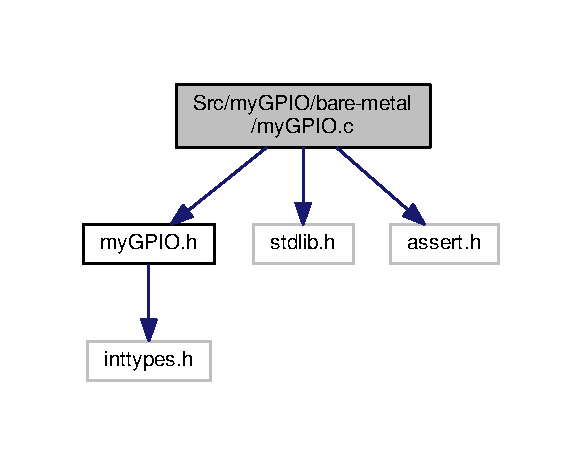
\includegraphics[width=280pt]{my_g_p_i_o_8c__incl}
\end{center}
\end{figure}
\subsection*{Funzioni}
\begin{DoxyCompactItemize}
\item 
void \hyperlink{group__bare-metal_ga588201358d1633c53535b288c9198531}{my\+G\+P\+I\+O\+\_\+\+Init} (\hyperlink{structmy_g_p_i_o__t}{my\+G\+P\+I\+O\+\_\+t} $\ast$gpio, uint32\+\_\+t base\+\_\+address)
\begin{DoxyCompactList}\small\item\em Inizializza un device my\+G\+P\+I\+O. \end{DoxyCompactList}\item 
void \hyperlink{group__bare-metal_ga43e82eb0febd452635a438fbd9cb853b}{my\+G\+P\+I\+O\+\_\+\+Set\+Mode} (\hyperlink{structmy_g_p_i_o__t}{my\+G\+P\+I\+O\+\_\+t} $\ast$gpio, \hyperlink{group__bare-metal_ga402a0d20afc0cb7c25554b8b023f4253}{my\+G\+P\+I\+O\+\_\+mask} mask, \hyperlink{group__bare-metal_ga76b849f0e0c05e7f9161bdb33396f2b1}{my\+G\+P\+I\+O\+\_\+mode} mode)
\begin{DoxyCompactList}\small\item\em Permette di settare la modalita' lettura/scrittura dei pin di un device my\+G\+P\+I\+O;. \end{DoxyCompactList}\item 
void \hyperlink{group__bare-metal_ga9d9ce9d2db7d77a588da4a3749f2f24d}{my\+G\+P\+I\+O\+\_\+\+Set\+Value} (\hyperlink{structmy_g_p_i_o__t}{my\+G\+P\+I\+O\+\_\+t} $\ast$gpio, \hyperlink{group__bare-metal_ga402a0d20afc0cb7c25554b8b023f4253}{my\+G\+P\+I\+O\+\_\+mask} mask, \hyperlink{group__bare-metal_gaf634fe4a0e1eab8da5000b72d6ad362b}{my\+G\+P\+I\+O\+\_\+value} value)
\begin{DoxyCompactList}\small\item\em Permette di settare il valore dei pin di un device my\+G\+P\+I\+O, se configurati come output. \end{DoxyCompactList}\item 
void \hyperlink{group__bare-metal_ga449b2af7cc20d24e6f6e017cf792ce03}{my\+G\+P\+I\+O\+\_\+\+Toggle} (\hyperlink{structmy_g_p_i_o__t}{my\+G\+P\+I\+O\+\_\+t} $\ast$gpio, \hyperlink{group__bare-metal_ga402a0d20afc0cb7c25554b8b023f4253}{my\+G\+P\+I\+O\+\_\+mask} mask)
\begin{DoxyCompactList}\small\item\em Permette di invertire il valore dei pin di un device my\+G\+P\+I\+O, se configurati come output. \end{DoxyCompactList}\item 
\hyperlink{group__bare-metal_gaf634fe4a0e1eab8da5000b72d6ad362b}{my\+G\+P\+I\+O\+\_\+value} \hyperlink{group__bare-metal_ga2a20e519816733b90204b975edc4e212}{my\+G\+P\+I\+O\+\_\+\+Get\+Value} (\hyperlink{structmy_g_p_i_o__t}{my\+G\+P\+I\+O\+\_\+t} $\ast$gpio, \hyperlink{group__bare-metal_ga402a0d20afc0cb7c25554b8b023f4253}{my\+G\+P\+I\+O\+\_\+mask} mask)
\begin{DoxyCompactList}\small\item\em Permette di leggere il valore dei pin di un device my\+G\+P\+I\+O;. \end{DoxyCompactList}\item 
\hyperlink{group__bare-metal_ga402a0d20afc0cb7c25554b8b023f4253}{my\+G\+P\+I\+O\+\_\+mask} \hyperlink{group__bare-metal_gac35776cd6652f7b932a132f3f6959a11}{my\+G\+P\+I\+O\+\_\+\+Get\+Read} (\hyperlink{structmy_g_p_i_o__t}{my\+G\+P\+I\+O\+\_\+t} $\ast$gpio)
\begin{DoxyCompactList}\small\item\em Restituisce la maschera dei pin settati di un device my\+G\+P\+I\+O. \end{DoxyCompactList}\item 
void \hyperlink{group__bare-metal_gada93ef6a9818e634f0a233ce14582216}{my\+G\+P\+I\+O\+\_\+\+Global\+Interrupt\+Enable} (\hyperlink{structmy_g_p_i_o__t}{my\+G\+P\+I\+O\+\_\+t} $\ast$gpio)
\begin{DoxyCompactList}\small\item\em Abilita gli interrupt globali;. \end{DoxyCompactList}\item 
void \hyperlink{group__bare-metal_gaacca2871ac57a166e62bf431a2da7548}{my\+G\+P\+I\+O\+\_\+\+Global\+Interrupt\+Disable} (\hyperlink{structmy_g_p_i_o__t}{my\+G\+P\+I\+O\+\_\+t} $\ast$gpio)
\begin{DoxyCompactList}\small\item\em Disabilita gli interrupt globali;. \end{DoxyCompactList}\item 
\hyperlink{group__bare-metal_gaf634fe4a0e1eab8da5000b72d6ad362b}{my\+G\+P\+I\+O\+\_\+value} \hyperlink{group__bare-metal_ga0a753db3d02ad08014e4b7304e0f1829}{my\+G\+P\+I\+O\+\_\+\+Is\+Global\+Interrupt\+Enabled} (\hyperlink{structmy_g_p_i_o__t}{my\+G\+P\+I\+O\+\_\+t} $\ast$gpio)
\begin{DoxyCompactList}\small\item\em Consente di verificare se gli interrupt globali siano abilitati. \end{DoxyCompactList}\item 
\hyperlink{group__bare-metal_gaf634fe4a0e1eab8da5000b72d6ad362b}{my\+G\+P\+I\+O\+\_\+value} \hyperlink{group__bare-metal_ga386cea84aca8c6bb731b4b46fcbf9199}{my\+G\+P\+I\+O\+\_\+\+Pending\+Interrupt} (\hyperlink{structmy_g_p_i_o__t}{my\+G\+P\+I\+O\+\_\+t} $\ast$gpio)
\begin{DoxyCompactList}\small\item\em Consente di verificare se esistano interrupt non ancora serviti. \end{DoxyCompactList}\item 
void \hyperlink{group__bare-metal_ga116e3a1077a317e9e42ded6dd4df64af}{my\+G\+P\+I\+O\+\_\+\+Pin\+Interrupt\+Enable} (\hyperlink{structmy_g_p_i_o__t}{my\+G\+P\+I\+O\+\_\+t} $\ast$gpio, \hyperlink{group__bare-metal_ga402a0d20afc0cb7c25554b8b023f4253}{my\+G\+P\+I\+O\+\_\+mask} mask)
\begin{DoxyCompactList}\small\item\em Abilita gli interrupt per i singoli pin del device. \end{DoxyCompactList}\item 
void \hyperlink{group__bare-metal_ga37d3df33ac50387d6f2e1fb5e2b13e49}{my\+G\+P\+I\+O\+\_\+\+Pin\+Interrupt\+Disable} (\hyperlink{structmy_g_p_i_o__t}{my\+G\+P\+I\+O\+\_\+t} $\ast$gpio, \hyperlink{group__bare-metal_ga402a0d20afc0cb7c25554b8b023f4253}{my\+G\+P\+I\+O\+\_\+mask} mask)
\begin{DoxyCompactList}\small\item\em Disabilita gli interrupt per i singoli pin del device. \end{DoxyCompactList}\item 
\hyperlink{group__bare-metal_ga402a0d20afc0cb7c25554b8b023f4253}{my\+G\+P\+I\+O\+\_\+mask} \hyperlink{group__bare-metal_ga80ef1cf3e9bd8bfd4d849a0f3b8e7b2c}{my\+G\+P\+I\+O\+\_\+\+Enabled\+Pin\+Interrupt} (\hyperlink{structmy_g_p_i_o__t}{my\+G\+P\+I\+O\+\_\+t} $\ast$gpio)
\begin{DoxyCompactList}\small\item\em Consente di ottenere una maschera che indichi quali pin abbiano interrupt abilitati. \end{DoxyCompactList}\item 
\hyperlink{group__bare-metal_ga402a0d20afc0cb7c25554b8b023f4253}{my\+G\+P\+I\+O\+\_\+mask} \hyperlink{group__bare-metal_ga6115bde39f860d4e76e7d8f421ce222c}{my\+G\+P\+I\+O\+\_\+\+Pending\+Pin\+Interrupt} (\hyperlink{structmy_g_p_i_o__t}{my\+G\+P\+I\+O\+\_\+t} $\ast$gpio)
\begin{DoxyCompactList}\small\item\em Consente di ottenere una maschera che indichi quali interrupt non siano stati ancora serviti;. \end{DoxyCompactList}\item 
void \hyperlink{group__bare-metal_gab6ad3dda867515825890c97dbf6f55db}{my\+G\+P\+I\+O\+\_\+\+Pin\+Interrupt\+Ack} (\hyperlink{structmy_g_p_i_o__t}{my\+G\+P\+I\+O\+\_\+t} $\ast$gpio, \hyperlink{group__bare-metal_ga402a0d20afc0cb7c25554b8b023f4253}{my\+G\+P\+I\+O\+\_\+mask} mask)
\begin{DoxyCompactList}\small\item\em Invia al device notifica di servizio di un interrupt;. \end{DoxyCompactList}\end{DoxyCompactItemize}


\subsection{Descrizione dettagliata}
\begin{DoxyAuthor}{Autore}
\+: Salvatore Barone \href{mailto:salvator.barone@gmail.com}{\tt salvator.\+barone@gmail.\+com} 
\end{DoxyAuthor}
\begin{DoxyDate}{Data}
\+: 12 05 2017
\end{DoxyDate}
\begin{DoxyCopyright}{Copyright}
Copyright 2017 Salvatore Barone \href{mailto:salvator.barone@gmail.com}{\tt salvator.\+barone@gmail.\+com}
\end{DoxyCopyright}
This file is part of Zynq7000\+Driver\+Pack

Zynq7000\+Driver\+Pack is free software; you can redistribute it and/or modify it under the terms of the G\+N\+U General Public License as published by the Free Software Foundation; either version 3 of the License, or any later version.

Zynq7000\+Driver\+Pack is distributed in the hope that it will be useful, but W\+I\+T\+H\+O\+U\+T A\+N\+Y W\+A\+R\+R\+A\+N\+T\+Y; without even the implied warranty of M\+E\+R\+C\+H\+A\+N\+T\+A\+B\+I\+L\+I\+T\+Y or F\+I\+T\+N\+E\+S\+S F\+O\+R A P\+A\+R\+T\+I\+C\+U\+L\+A\+R P\+U\+R\+P\+O\+S\+E. See the G\+N\+U General Public License for more details.

You should have received a copy of the G\+N\+U General Public License along with this program; if not, write to the Free Software Foundation, Inc., 51 Franklin Street, Fifth Floor, Boston, M\+A 02110-\/1301, U\+S\+A. 
\hypertarget{my_g_p_i_o_8h}{\section{Riferimenti per il file my\+G\+P\+I\+O/my\+G\+P\+I\+O.h}
\label{my_g_p_i_o_8h}\index{my\+G\+P\+I\+O/my\+G\+P\+I\+O.\+h@{my\+G\+P\+I\+O/my\+G\+P\+I\+O.\+h}}
}
{\ttfamily \#include $<$inttypes.\+h$>$}\\*
Grafo delle dipendenze di inclusione per my\+G\+P\+I\+O.\+h\+:\nopagebreak
\begin{figure}[H]
\begin{center}
\leavevmode
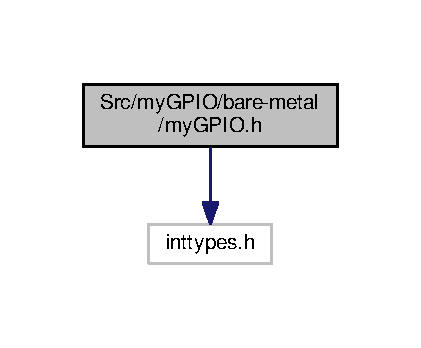
\includegraphics[width=184pt]{my_g_p_i_o_8h__incl}
\end{center}
\end{figure}
Questo grafo mostra quali altri file includono direttamente o indirettamente questo file\+:\nopagebreak
\begin{figure}[H]
\begin{center}
\leavevmode
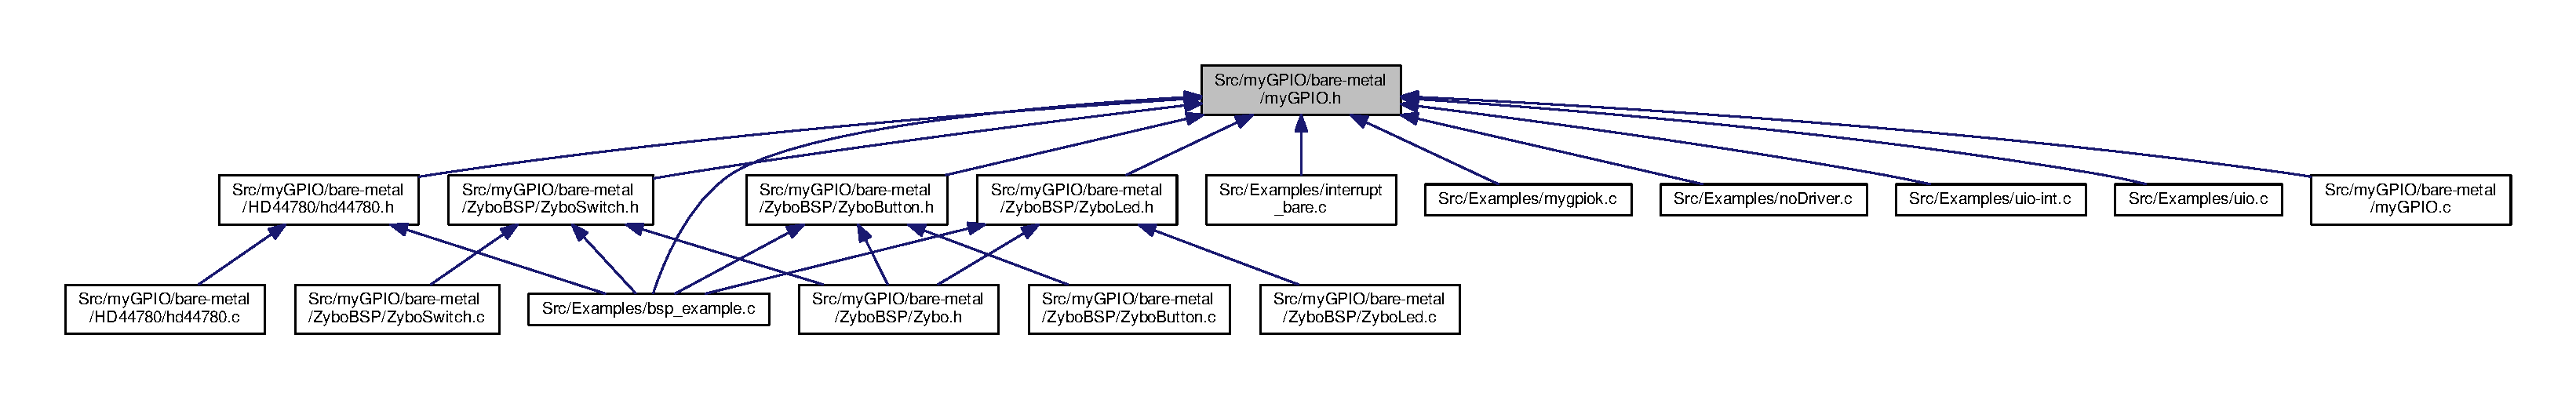
\includegraphics[width=350pt]{my_g_p_i_o_8h__dep__incl}
\end{center}
\end{figure}
\subsection*{Strutture dati}
\begin{DoxyCompactItemize}
\item 
struct \hyperlink{structmy_g_p_i_o__t}{my\+G\+P\+I\+O\+\_\+t}
\begin{DoxyCompactList}\small\item\em Struttura che astrae un device my\+G\+P\+I\+O. \end{DoxyCompactList}\end{DoxyCompactItemize}
\subsection*{Definizioni}
\begin{DoxyCompactItemize}
\item 
\#define \hyperlink{group__my_g_p_i_o_ga81a662103d6ed053978c0a9b4c273065}{my\+G\+P\+I\+O\+\_\+\+M\+O\+D\+E\+\_\+\+O\+F\+F\+S\+E\+T}~0\+U
\begin{DoxyCompactList}\small\item\em Offset, rispetto all'indirizzo base, del registro \char`\"{}mode\char`\"{} per il device my\+G\+P\+I\+O. \end{DoxyCompactList}\item 
\#define \hyperlink{group__my_g_p_i_o_ga2e45778b6ca9ce6f5768b3f7a4557ce1}{my\+G\+P\+I\+O\+\_\+\+W\+R\+I\+T\+E\+\_\+\+O\+F\+F\+S\+E\+T}~4\+U
\begin{DoxyCompactList}\small\item\em Offset, rispetto all'indirizzo base, del registro \char`\"{}write\char`\"{} per il device my\+G\+P\+I\+O. \end{DoxyCompactList}\item 
\#define \hyperlink{group__my_g_p_i_o_ga584d2dfece76e5762030d918d80592cc}{my\+G\+P\+I\+O\+\_\+\+R\+E\+A\+D\+\_\+\+O\+F\+F\+S\+E\+T}~8\+U
\begin{DoxyCompactList}\small\item\em Offset, rispetto all'indirizzo base, del registro \char`\"{}read\char`\"{} per il device my\+G\+P\+I\+O. \end{DoxyCompactList}\item 
\#define \hyperlink{group__my_g_p_i_o_gaacf2d8a21a051e778f02f8811b9c1e96}{my\+G\+P\+I\+O\+\_\+\+I\+N\+T\+R\+\_\+\+O\+F\+F\+S\+E\+T}~12\+U
\begin{DoxyCompactList}\small\item\em Offset, rispetto all'indirizzo base, del registro \char`\"{}interrupt\char`\"{} per il device my\+G\+P\+I\+O. \end{DoxyCompactList}\item 
\#define \hyperlink{group__my_g_p_i_o_ga0ba32e2adf874ed7216c5993369153e1}{my\+G\+P\+I\+O\+\_\+\+I\+N\+T\+R\+\_\+\+Int\+En\+\_\+mask}~0x1\+U
\begin{DoxyCompactList}\small\item\em maschera del bit del registro \char`\"{}interrupt\char`\"{} che funge da interrupt-\/enable, per il device my\+G\+P\+I\+O \end{DoxyCompactList}\item 
\#define \hyperlink{group__my_g_p_i_o_ga4cd02635783bc2a4ad7639cfb9fdb698}{my\+G\+P\+I\+O\+\_\+\+I\+N\+T\+R\+\_\+\+Irq\+\_\+mask}~0x2\+U
\begin{DoxyCompactList}\small\item\em maschera del bit del registro \char`\"{}interrupt\char`\"{} che funge da interrupt-\/request, per il device my\+G\+P\+I\+O \end{DoxyCompactList}\item 
\#define \hyperlink{group__my_g_p_i_o_gaa760b8397e6372e48c1008c2ba8d7387}{my\+G\+P\+I\+O\+\_\+\+I\+N\+T\+R\+\_\+\+Int\+Ack\+\_\+mask}~0x4\+U
\begin{DoxyCompactList}\small\item\em maschera del bit del registro \char`\"{}interrupt\char`\"{} che funge da interrupt-\/ack, per il device my\+G\+P\+I\+O \end{DoxyCompactList}\item 
\#define \hyperlink{group__my_g_p_i_o_gabbe2491a3b71c292521025b7b382b971}{my\+G\+P\+I\+O\+\_\+pin}(i)~((uint32\+\_\+t)(1$<$$<$(i)))
\begin{DoxyCompactList}\small\item\em Metodo alternativo per la specifica di uno dei pin di un device my\+G\+P\+I\+O. \end{DoxyCompactList}\end{DoxyCompactItemize}
\subsection*{Tipi enumerati (enum)}
\begin{DoxyCompactItemize}
\item 
enum \hyperlink{group__my_g_p_i_o_ga402a0d20afc0cb7c25554b8b023f4253}{my\+G\+P\+I\+O\+\_\+mask} \{ \\*
\hyperlink{group__my_g_p_i_o_gga402a0d20afc0cb7c25554b8b023f4253a6db6fa7be955ae379f543d96122e23a9}{my\+G\+P\+I\+O\+\_\+pin0} = 0x1\+U, 
\hyperlink{group__my_g_p_i_o_gga402a0d20afc0cb7c25554b8b023f4253a1de6bdcc01efca2c39f584f5a20293be}{my\+G\+P\+I\+O\+\_\+pin1} = 0x2\+U, 
\hyperlink{group__my_g_p_i_o_gga402a0d20afc0cb7c25554b8b023f4253a1fb3f52d920ac8ba17b74dd73c27d783}{my\+G\+P\+I\+O\+\_\+pin2} = 0x4\+U, 
\hyperlink{group__my_g_p_i_o_gga402a0d20afc0cb7c25554b8b023f4253a4514d64390392b626aa4dbfaac8dc1e5}{my\+G\+P\+I\+O\+\_\+pin3} = 0x8\+U, 
\\*
\hyperlink{group__my_g_p_i_o_gga402a0d20afc0cb7c25554b8b023f4253a0a446f53dee6f6f4ccb9a1d1f947b637}{my\+G\+P\+I\+O\+\_\+pin4} = 0x10\+U, 
\hyperlink{group__my_g_p_i_o_gga402a0d20afc0cb7c25554b8b023f4253a04a111036a27e9b97f0950f6d37b04d2}{my\+G\+P\+I\+O\+\_\+pin5} = 0x20\+U, 
\hyperlink{group__my_g_p_i_o_gga402a0d20afc0cb7c25554b8b023f4253a39a529f8c0a4f302029f54daa815471b}{my\+G\+P\+I\+O\+\_\+pin6} = 0x40\+U, 
\hyperlink{group__my_g_p_i_o_gga402a0d20afc0cb7c25554b8b023f4253af4e88b077442e4c0f459e1e4aa60626b}{my\+G\+P\+I\+O\+\_\+pin7} = 0x80\+U, 
\\*
\hyperlink{group__my_g_p_i_o_gga402a0d20afc0cb7c25554b8b023f4253a615159bcf4e347dc2b60f2545fae5f9e}{my\+G\+P\+I\+O\+\_\+pin8} = 0x100\+U, 
\hyperlink{group__my_g_p_i_o_gga402a0d20afc0cb7c25554b8b023f4253a8d721236fb936126a08c12b87696f6e9}{my\+G\+P\+I\+O\+\_\+pin9} = 0x200\+U, 
\hyperlink{group__my_g_p_i_o_gga402a0d20afc0cb7c25554b8b023f4253ae3067b7b3b1a2e171ecd74b6abd48341}{my\+G\+P\+I\+O\+\_\+pin10} = 0x400\+U, 
\hyperlink{group__my_g_p_i_o_gga402a0d20afc0cb7c25554b8b023f4253ae5c2e65508bfd452100d9da331d6220a}{my\+G\+P\+I\+O\+\_\+pin11} = 0x800\+U, 
\\*
\hyperlink{group__my_g_p_i_o_gga402a0d20afc0cb7c25554b8b023f4253afa75e3c1c019048c8553cb733c5137b5}{my\+G\+P\+I\+O\+\_\+pin12} = 0x1000\+U, 
\hyperlink{group__my_g_p_i_o_gga402a0d20afc0cb7c25554b8b023f4253a243381a796f0936a576f184dd115b37c}{my\+G\+P\+I\+O\+\_\+pin13} = 0x2000\+U, 
\hyperlink{group__my_g_p_i_o_gga402a0d20afc0cb7c25554b8b023f4253aed4915d6b3eab49cc1ba971b9f439fdd}{my\+G\+P\+I\+O\+\_\+pin14} = 0x4000\+U, 
\hyperlink{group__my_g_p_i_o_gga402a0d20afc0cb7c25554b8b023f4253a46c427ea97182a77e8c975d3429a64ee}{my\+G\+P\+I\+O\+\_\+pin15} = 0x8000\+U, 
\\*
\hyperlink{group__my_g_p_i_o_gga402a0d20afc0cb7c25554b8b023f4253a5a27c4d87207b2eba865876854f1ba67}{my\+G\+P\+I\+O\+\_\+pin16} = 0x10000\+U, 
\hyperlink{group__my_g_p_i_o_gga402a0d20afc0cb7c25554b8b023f4253ab0541af31059bdc8dca44d5dafa7e779}{my\+G\+P\+I\+O\+\_\+pin17} = 0x20000\+U, 
\hyperlink{group__my_g_p_i_o_gga402a0d20afc0cb7c25554b8b023f4253a7a51a492e3cb580581a2c8eb439edd99}{my\+G\+P\+I\+O\+\_\+pin18} = 0x40000\+U, 
\hyperlink{group__my_g_p_i_o_gga402a0d20afc0cb7c25554b8b023f4253a9118ae2775e93bd4522660e81a2d5309}{my\+G\+P\+I\+O\+\_\+pin19} = 0x80000\+U, 
\\*
\hyperlink{group__my_g_p_i_o_gga402a0d20afc0cb7c25554b8b023f4253a7940782a16f88dbbb3a4037c2bef1711}{my\+G\+P\+I\+O\+\_\+pin20} = 0x100000\+U, 
\hyperlink{group__my_g_p_i_o_gga402a0d20afc0cb7c25554b8b023f4253a1da616a8cf4396927db1e5a336fb6dc5}{my\+G\+P\+I\+O\+\_\+pin21} = 0x200000\+U, 
\hyperlink{group__my_g_p_i_o_gga402a0d20afc0cb7c25554b8b023f4253acf80113da8d789f7da9f9edc4ab6003c}{my\+G\+P\+I\+O\+\_\+pin22} = 0x400000\+U, 
\hyperlink{group__my_g_p_i_o_gga402a0d20afc0cb7c25554b8b023f4253ad64e03b703608de173ab5950b5121830}{my\+G\+P\+I\+O\+\_\+pin23} = 0x800000\+U, 
\\*
\hyperlink{group__my_g_p_i_o_gga402a0d20afc0cb7c25554b8b023f4253a5bb93f546327123f81b06ed0dfcdf110}{my\+G\+P\+I\+O\+\_\+pin24} = 0x1000000\+U, 
\hyperlink{group__my_g_p_i_o_gga402a0d20afc0cb7c25554b8b023f4253a0b27a7e78aff5836f33085f3b4539f56}{my\+G\+P\+I\+O\+\_\+pin25} = 0x2000000\+U, 
\hyperlink{group__my_g_p_i_o_gga402a0d20afc0cb7c25554b8b023f4253aaa07c24140250dcbc695206793efa8af}{my\+G\+P\+I\+O\+\_\+pin26} = 0x4000000\+U, 
\hyperlink{group__my_g_p_i_o_gga402a0d20afc0cb7c25554b8b023f4253a1dd5e99eba6237aeb30b2194c553c37f}{my\+G\+P\+I\+O\+\_\+pin27} = 0x8000000\+U, 
\\*
\hyperlink{group__my_g_p_i_o_gga402a0d20afc0cb7c25554b8b023f4253a2076590efec8bcf9ef3285798753e632}{my\+G\+P\+I\+O\+\_\+pin28} = 0x10000000\+U, 
\hyperlink{group__my_g_p_i_o_gga402a0d20afc0cb7c25554b8b023f4253abfe9540fa3946a35e20f7f68cb1b8084}{my\+G\+P\+I\+O\+\_\+pin29} = 0x20000000\+U, 
\hyperlink{group__my_g_p_i_o_gga402a0d20afc0cb7c25554b8b023f4253a59993a30c537c116eddb42d10778f4f8}{my\+G\+P\+I\+O\+\_\+pin30} = 0x40000000\+U, 
\hyperlink{group__my_g_p_i_o_gga402a0d20afc0cb7c25554b8b023f4253a9a55b7c245bd9aad750b7891d27e9225}{my\+G\+P\+I\+O\+\_\+pin31} = 0x80000000\+U, 
\\*
\hyperlink{group__my_g_p_i_o_gga402a0d20afc0cb7c25554b8b023f4253a0347b1742eef6b2575a7d409c7fb5c3d}{my\+G\+P\+I\+O\+\_\+byte0} = 0x000000ff\+U, 
\hyperlink{group__my_g_p_i_o_gga402a0d20afc0cb7c25554b8b023f4253ae5aec65fa20f554b893e419fc2755fd0}{my\+G\+P\+I\+O\+\_\+byte1} = 0x0000ff00\+U, 
\hyperlink{group__my_g_p_i_o_gga402a0d20afc0cb7c25554b8b023f4253af4892f7db28c64a7cf2a7236c88b742b}{my\+G\+P\+I\+O\+\_\+byte2} = 0x00ff0000\+U, 
\hyperlink{group__my_g_p_i_o_gga402a0d20afc0cb7c25554b8b023f4253a1ceefb9d65397352e986c573984d0129}{my\+G\+P\+I\+O\+\_\+byte3} = 0xff000000\+U
 \}
\begin{DoxyCompactList}\small\item\em Maschere di selezione dei pin di un device my\+G\+P\+I\+O. \end{DoxyCompactList}\item 
enum \hyperlink{group__my_g_p_i_o_ga76b849f0e0c05e7f9161bdb33396f2b1}{my\+G\+P\+I\+O\+\_\+mode} \{ \hyperlink{group__my_g_p_i_o_gga76b849f0e0c05e7f9161bdb33396f2b1a1e6dc78e7641e878cadc842d39605d5d}{my\+G\+P\+I\+O\+\_\+read}, 
\hyperlink{group__my_g_p_i_o_gga76b849f0e0c05e7f9161bdb33396f2b1a2d66976280eb7595a42c631683bdfad6}{my\+G\+P\+I\+O\+\_\+write}
 \}
\begin{DoxyCompactList}\small\item\em my\+G\+P\+I\+O\+\_\+mode, modalita' di funzionamento (lettura/scrittura) di un device my\+G\+P\+I\+O \end{DoxyCompactList}\item 
enum \hyperlink{group__my_g_p_i_o_gaf634fe4a0e1eab8da5000b72d6ad362b}{my\+G\+P\+I\+O\+\_\+value} \{ \hyperlink{group__my_g_p_i_o_ggaf634fe4a0e1eab8da5000b72d6ad362ba98cde80dbda025bd1ae7231c76b55674}{my\+G\+P\+I\+O\+\_\+reset}, 
\hyperlink{group__my_g_p_i_o_ggaf634fe4a0e1eab8da5000b72d6ad362ba10d296f3711d01189cc6c2d87f7c9149}{my\+G\+P\+I\+O\+\_\+set}
 \}
\begin{DoxyCompactList}\small\item\em my\+G\+P\+I\+O\+\_\+value, valore di un my\+G\+P\+I\+O \end{DoxyCompactList}\end{DoxyCompactItemize}
\subsection*{Funzioni}
\begin{DoxyCompactItemize}
\item 
void \hyperlink{group__my_g_p_i_o_ga8fda7ca73b187baf256409423c25d725}{my\+G\+P\+I\+O\+\_\+init} (\hyperlink{structmy_g_p_i_o__t}{my\+G\+P\+I\+O\+\_\+t} $\ast$gpio, uint32\+\_\+t base\+\_\+address)
\begin{DoxyCompactList}\small\item\em Inizializza un device my\+G\+P\+I\+O. \end{DoxyCompactList}\item 
void \hyperlink{group__my_g_p_i_o_ga38a2ea04d07af50f7f570f0367594c8b}{my\+G\+P\+I\+O\+\_\+set\+Mode} (\hyperlink{structmy_g_p_i_o__t}{my\+G\+P\+I\+O\+\_\+t} $\ast$gpio, \hyperlink{group__my_g_p_i_o_ga402a0d20afc0cb7c25554b8b023f4253}{my\+G\+P\+I\+O\+\_\+mask} mask, \hyperlink{group__my_g_p_i_o_ga76b849f0e0c05e7f9161bdb33396f2b1}{my\+G\+P\+I\+O\+\_\+mode} mode)
\begin{DoxyCompactList}\small\item\em Permette di settare la modalita' lettura/scrittura dei pin di un device my\+G\+P\+I\+O;. \end{DoxyCompactList}\item 
void \hyperlink{group__my_g_p_i_o_gab742e68093ad4c90fe299b64fd6736ca}{my\+G\+P\+I\+O\+\_\+set\+Value} (\hyperlink{structmy_g_p_i_o__t}{my\+G\+P\+I\+O\+\_\+t} $\ast$gpio, \hyperlink{group__my_g_p_i_o_ga402a0d20afc0cb7c25554b8b023f4253}{my\+G\+P\+I\+O\+\_\+mask} mask, \hyperlink{group__my_g_p_i_o_gaf634fe4a0e1eab8da5000b72d6ad362b}{my\+G\+P\+I\+O\+\_\+value} value)
\begin{DoxyCompactList}\small\item\em Permette di settare il valore dei pin di un device my\+G\+P\+I\+O, se configurati come output. \end{DoxyCompactList}\item 
void \hyperlink{group__my_g_p_i_o_ga27ea411bf51a58fe48eb8c5036780b53}{my\+G\+P\+I\+O\+\_\+toggle} (\hyperlink{structmy_g_p_i_o__t}{my\+G\+P\+I\+O\+\_\+t} $\ast$gpio, \hyperlink{group__my_g_p_i_o_ga402a0d20afc0cb7c25554b8b023f4253}{my\+G\+P\+I\+O\+\_\+mask} mask)
\begin{DoxyCompactList}\small\item\em Permette di invertire il valore dei pin di un device my\+G\+P\+I\+O, se configurati come output. \end{DoxyCompactList}\item 
\hyperlink{group__my_g_p_i_o_gaf634fe4a0e1eab8da5000b72d6ad362b}{my\+G\+P\+I\+O\+\_\+value} \hyperlink{group__my_g_p_i_o_gad6576f1d0fb17d9b492da0b1008550d0}{my\+G\+P\+I\+O\+\_\+get\+Value} (\hyperlink{structmy_g_p_i_o__t}{my\+G\+P\+I\+O\+\_\+t} $\ast$gpio, \hyperlink{group__my_g_p_i_o_ga402a0d20afc0cb7c25554b8b023f4253}{my\+G\+P\+I\+O\+\_\+mask} mask)
\begin{DoxyCompactList}\small\item\em Permette di leggere il valore dei pin di un device my\+G\+P\+I\+O;. \end{DoxyCompactList}\item 
\hyperlink{group__my_g_p_i_o_ga402a0d20afc0cb7c25554b8b023f4253}{my\+G\+P\+I\+O\+\_\+mask} \hyperlink{group__my_g_p_i_o_gadb3ecd03ea82420488977134c9313e18}{my\+G\+P\+I\+O\+\_\+get\+Read} (\hyperlink{structmy_g_p_i_o__t}{my\+G\+P\+I\+O\+\_\+t} $\ast$gpio)
\begin{DoxyCompactList}\small\item\em Restituisce la maschera dei pin settati di un device my\+G\+P\+I\+O. \end{DoxyCompactList}\item 
void \hyperlink{group__my_g_p_i_o_ga39822bfa495a9388e81ced74884c06a2}{my\+G\+P\+I\+O\+\_\+interrupt\+Enable} (\hyperlink{structmy_g_p_i_o__t}{my\+G\+P\+I\+O\+\_\+t} $\ast$gpio)
\begin{DoxyCompactList}\small\item\em Abilita gli interrupt per un device my\+G\+P\+I\+O. \end{DoxyCompactList}\item 
void \hyperlink{group__my_g_p_i_o_gab681db0119860bfad2c3e674289d8b3d}{my\+G\+P\+I\+O\+\_\+interrupt\+Disable} (\hyperlink{structmy_g_p_i_o__t}{my\+G\+P\+I\+O\+\_\+t} $\ast$gpio)
\begin{DoxyCompactList}\small\item\em Disabilita gli interrupt per un device my\+G\+P\+I\+O. \end{DoxyCompactList}\item 
void \hyperlink{group__my_g_p_i_o_ga396f6e5e7f0eeff01e98fcc78523402b}{my\+G\+P\+I\+O\+\_\+interrupt\+Ack} (\hyperlink{structmy_g_p_i_o__t}{my\+G\+P\+I\+O\+\_\+t} $\ast$gpio)
\begin{DoxyCompactList}\small\item\em Segnala al device che l'interruzione da lui sollevata e' stata servita. \end{DoxyCompactList}\item 
\hyperlink{group__my_g_p_i_o_gaf634fe4a0e1eab8da5000b72d6ad362b}{my\+G\+P\+I\+O\+\_\+value} \hyperlink{group__my_g_p_i_o_ga7936b506b45f116de68ddf06c84cc242}{my\+G\+P\+I\+O\+\_\+get\+Irq} (\hyperlink{structmy_g_p_i_o__t}{my\+G\+P\+I\+O\+\_\+t} $\ast$gpio)
\begin{DoxyCompactList}\small\item\em Consente di verificare se un device my\+G\+P\+I\+O abbia generato un'interruzione. \end{DoxyCompactList}\end{DoxyCompactItemize}


\subsection{Descrizione dettagliata}
\begin{DoxyAuthor}{Autore}
\+: Salvatore Barone \href{mailto:salvator.barone@gmail.com}{\tt salvator.\+barone@gmail.\+com} 
\end{DoxyAuthor}
\begin{DoxyDate}{Data}
\+: 12 05 2017
\end{DoxyDate}
\begin{DoxyCopyright}{Copyright}
Copyright 2017 Salvatore Barone \href{mailto:salvator.barone@gmail.com}{\tt salvator.\+barone@gmail.\+com}
\end{DoxyCopyright}
This file is part of Zynq7000\+Driver\+Pack

Zynq7000\+Driver\+Pack is free software; you can redistribute it and/or modify it under the terms of the G\+N\+U General Public License as published by the Free Software Foundation; either version 3 of the License, or any later version.

Zynq7000\+Driver\+Pack is distributed in the hope that it will be useful, but W\+I\+T\+H\+O\+U\+T A\+N\+Y W\+A\+R\+R\+A\+N\+T\+Y; without even the implied warranty of M\+E\+R\+C\+H\+A\+N\+T\+A\+B\+I\+L\+I\+T\+Y or F\+I\+T\+N\+E\+S\+S F\+O\+R A P\+A\+R\+T\+I\+C\+U\+L\+A\+R P\+U\+R\+P\+O\+S\+E. See the G\+N\+U General Public License for more details.

You should have received a copy of the G\+N\+U General Public License along with this program; if not, write to the Free Software Foundation, Inc., 51 Franklin Street, Fifth Floor, Boston, M\+A 02110-\/1301, U\+S\+A. 
\hypertarget{_zybo_8h}{}\section{Riferimenti per il file Src/my\+G\+P\+I\+O/bare-\/metal/\+Zybo\+B\+S\+P/\+Zybo.h}
\label{_zybo_8h}\index{Src/my\+G\+P\+I\+O/bare-\/metal/\+Zybo\+B\+S\+P/\+Zybo.\+h@{Src/my\+G\+P\+I\+O/bare-\/metal/\+Zybo\+B\+S\+P/\+Zybo.\+h}}
{\ttfamily \#include \char`\"{}Zybo\+Led.\+h\char`\"{}}\newline
{\ttfamily \#include \char`\"{}Zybo\+Switch.\+h\char`\"{}}\newline
{\ttfamily \#include \char`\"{}Zybo\+Button.\+h\char`\"{}}\newline
Grafo delle dipendenze di inclusione per Zybo.\+h\+:\nopagebreak
\begin{figure}[H]
\begin{center}
\leavevmode
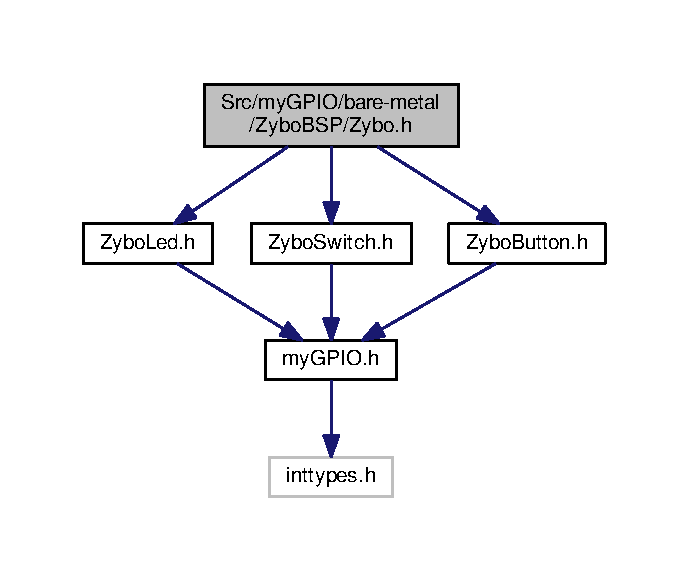
\includegraphics[width=331pt]{_zybo_8h__incl}
\end{center}
\end{figure}


\subsection{Descrizione dettagliata}
\begin{DoxyAuthor}{Autore}
Salvatore Barone \href{mailto:salvator.barone@gmail.com}{\tt salvator.\+barone@gmail.\+com}
\end{DoxyAuthor}
\begin{DoxyCopyright}{Copyright}
Copyright 2017 Salvatore Barone \href{mailto:salvator.barone@gmail.com}{\tt salvator.\+barone@gmail.\+com}
\end{DoxyCopyright}
This file is part of Zynq7000\+Driver\+Pack

Zynq7000\+Driver\+Pack is free software; you can redistribute it and/or modify it under the terms of the G\+NU General Public License as published by the Free Software Foundation; either version 3 of the License, or any later version.

Zynq7000\+Driver\+Pack is distributed in the hope that it will be useful, but W\+I\+T\+H\+O\+UT A\+NY W\+A\+R\+R\+A\+N\+TY; without even the implied warranty of M\+E\+R\+C\+H\+A\+N\+T\+A\+B\+I\+L\+I\+TY or F\+I\+T\+N\+E\+SS F\+OR A P\+A\+R\+T\+I\+C\+U\+L\+AR P\+U\+R\+P\+O\+SE. See the G\+NU General Public License for more details.

You should have received a copy of the G\+NU General Public License along with this program; if not, write to the Free Software Foundation, Inc., 51 Franklin Street, Fifth Floor, Boston, MA 02110-\/1301, U\+SA. 
\hypertarget{_zybo_button_8c}{\section{Riferimenti per il file Zybo/\+Zybo\+Button.c}
\label{_zybo_button_8c}\index{Zybo/\+Zybo\+Button.\+c@{Zybo/\+Zybo\+Button.\+c}}
}
{\ttfamily \#include \char`\"{}Zybo\+Button.\+h\char`\"{}}\\*
{\ttfamily \#include $<$assert.\+h$>$}\\*
{\ttfamily \#include $<$stdlib.\+h$>$}\\*
Grafo delle dipendenze di inclusione per Zybo\+Button.\+c\+:
\nopagebreak
\begin{figure}[H]
\begin{center}
\leavevmode
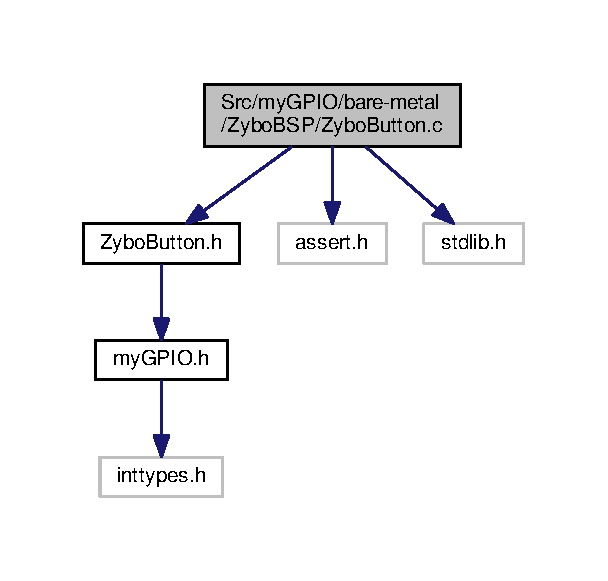
\includegraphics[width=292pt]{_zybo_button_8c__incl}
\end{center}
\end{figure}
\subsection*{Definizioni}
\begin{DoxyCompactItemize}
\item 
\#define \hyperlink{_zybo_button_8c_a5f45c877d1e8266f8a2c1d0b87746950}{timer\+\_\+wait\+\_\+ms}(ms)~usleep(ms$<$$<$10)
\end{DoxyCompactItemize}
\subsection*{Funzioni}
\begin{DoxyCompactItemize}
\item 
void \hyperlink{group___button_gaa40462223af93b0f5bdf2932400fe2a5}{Zybo\+Button\+\_\+init} (\hyperlink{struct_zybo_button__t}{Zybo\+Button\+\_\+t} $\ast$buttons, G\+P\+I\+O\+\_\+t $\ast$gpio, G\+P\+I\+O\+\_\+mask Button3\+\_\+pin, G\+P\+I\+O\+\_\+mask Button2\+\_\+pin, G\+P\+I\+O\+\_\+mask Button1\+\_\+pin, G\+P\+I\+O\+\_\+mask Button0\+\_\+pin)
\begin{DoxyCompactList}\small\item\em Inizializza un oggetto di tipo \hyperlink{struct_zybo_button__t}{Zybo\+Button\+\_\+t}. \end{DoxyCompactList}\item 
void \hyperlink{group___button_gaca30e81084e746785e395f79e9678e9a}{Zybo\+Button\+\_\+wait\+While\+Idle} (\hyperlink{struct_zybo_button__t}{Zybo\+Button\+\_\+t} $\ast$buttons)
\begin{DoxyCompactList}\small\item\em Permettere di mettere il programma in attesa attiva finche' i button restano inattivi;. \end{DoxyCompactList}\item 
void \hyperlink{group___button_ga3840edf011b5bad6302b7efc9c6326fe}{Zybo\+Button\+\_\+wait\+While\+Busy} (\hyperlink{struct_zybo_button__t}{Zybo\+Button\+\_\+t} $\ast$buttons)
\begin{DoxyCompactList}\small\item\em Permettere di mettere il programma in attesa attiva finche' i button restano attivi;. \end{DoxyCompactList}\item 
\hyperlink{group___button_ga85c290bfa232cab213e69200bf78e06a}{Zybo\+Button\+\_\+status\+\_\+t} \hyperlink{group___button_ga75407539e8ba0ad3ea142496219cd083}{Zybo\+Button\+\_\+get\+Status} (\hyperlink{struct_zybo_button__t}{Zybo\+Button\+\_\+t} $\ast$buttons, \hyperlink{group___button_ga4d26a5f6cad606de534ba034e0ba42dd}{Zybo\+Button\+\_\+mask\+\_\+t} mask)
\begin{DoxyCompactList}\small\item\em Permette la lettura dello stato dei button presenti sulla board. \end{DoxyCompactList}\end{DoxyCompactItemize}


\subsection{Documentazione delle definizioni}
\hypertarget{_zybo_button_8c_a5f45c877d1e8266f8a2c1d0b87746950}{\index{Zybo\+Button.\+c@{Zybo\+Button.\+c}!timer\+\_\+wait\+\_\+ms@{timer\+\_\+wait\+\_\+ms}}
\index{timer\+\_\+wait\+\_\+ms@{timer\+\_\+wait\+\_\+ms}!Zybo\+Button.\+c@{Zybo\+Button.\+c}}
\subsubsection[{timer\+\_\+wait\+\_\+ms}]{\setlength{\rightskip}{0pt plus 5cm}\#define timer\+\_\+wait\+\_\+ms(
\begin{DoxyParamCaption}
\item[{}]{ms}
\end{DoxyParamCaption}
)~usleep(ms$<$$<$10)}}\label{_zybo_button_8c_a5f45c877d1e8266f8a2c1d0b87746950}

\hypertarget{_zybo_button_8h}{\section{Riferimenti per il file Zybo/\+Zybo\+Button.h}
\label{_zybo_button_8h}\index{Zybo/\+Zybo\+Button.\+h@{Zybo/\+Zybo\+Button.\+h}}
}
{\ttfamily \#include \char`\"{}gpio.\+h\char`\"{}}\\*
Grafo delle dipendenze di inclusione per Zybo\+Button.\+h\+:\nopagebreak
\begin{figure}[H]
\begin{center}
\leavevmode
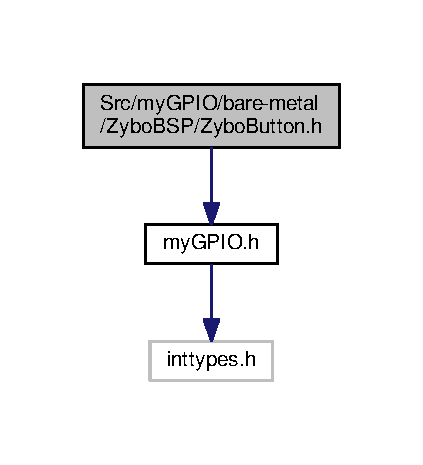
\includegraphics[width=180pt]{_zybo_button_8h__incl}
\end{center}
\end{figure}
Questo grafo mostra quali altri file includono direttamente o indirettamente questo file\+:\nopagebreak
\begin{figure}[H]
\begin{center}
\leavevmode
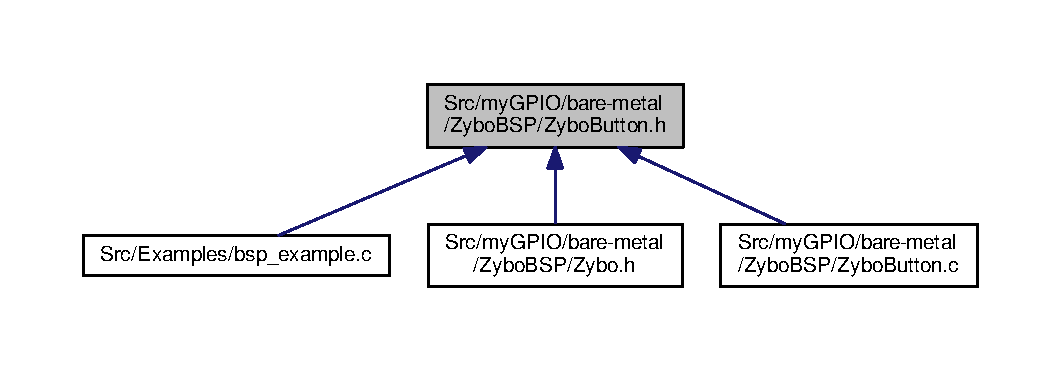
\includegraphics[width=270pt]{_zybo_button_8h__dep__incl}
\end{center}
\end{figure}
\subsection*{Strutture dati}
\begin{DoxyCompactItemize}
\item 
struct \hyperlink{struct_zybo_button__t}{Zybo\+Button\+\_\+t}
\begin{DoxyCompactList}\small\item\em Struttura opaca che astrae l'insieme dei button presenti sulla board Digilent Zybo;. \end{DoxyCompactList}\end{DoxyCompactItemize}
\subsection*{Definizioni}
\begin{DoxyCompactItemize}
\item 
\#define \hyperlink{group___button_ga5f85cbc14732f1d83faa75500b67defa}{Zybo\+Button}(i)~((uint32\+\_\+t)(1$<$$<$i))
\begin{DoxyCompactList}\small\item\em Metodo alternativo per la specifica di uno dei button presenti sulla board Digilent Zybo. \end{DoxyCompactList}\item 
\#define \hyperlink{group___button_ga8960eefa6a431f50d4fe2a2f8063da3f}{Zybo\+Button\+\_\+\+Debounce\+Wait}~50
\begin{DoxyCompactList}\small\item\em Tempo di attesa (in millisecondi) usato per prevenire il fenomeno del bouncing. Il valore di default è 50, determinato empiricamente. Puo' essere modificato a piacimento cambiando il valore alla macro seguente. \end{DoxyCompactList}\end{DoxyCompactItemize}
\subsection*{Tipi enumerati (enum)}
\begin{DoxyCompactItemize}
\item 
enum \hyperlink{group___button_ga4d26a5f6cad606de534ba034e0ba42dd}{Zybo\+Button\+\_\+mask\+\_\+t} \{ \hyperlink{group___button_gga4d26a5f6cad606de534ba034e0ba42ddaabede392be8cae14b8a070a804c754e8}{Zybo\+Button3} = 0x8, 
\hyperlink{group___button_gga4d26a5f6cad606de534ba034e0ba42dda2aa888c8f01ac8a79013e5ebc9eef609}{Zybo\+Button2} = 0x4, 
\hyperlink{group___button_gga4d26a5f6cad606de534ba034e0ba42dda29c35ef3133898c050f675a60de66dd7}{Zybo\+Button1} = 0x2, 
\hyperlink{group___button_gga4d26a5f6cad606de534ba034e0ba42dda2f821ce9661687aefb0ec4de65911570}{Zybo\+Button0} = 0x1
 \}
\begin{DoxyCompactList}\small\item\em Maschere di selezione dei Push\+Button. \end{DoxyCompactList}\item 
enum \hyperlink{group___button_ga85c290bfa232cab213e69200bf78e06a}{Zybo\+Button\+\_\+status\+\_\+t} \{ \hyperlink{group___button_gga85c290bfa232cab213e69200bf78e06aacd110f28912806bcec929721e8737399}{Zybo\+Button\+\_\+off}, 
\hyperlink{group___button_gga85c290bfa232cab213e69200bf78e06aa49bf4a6902270f28bc6a1146fbd1b1fe}{Zybo\+Button\+\_\+on}
 \}
\begin{DoxyCompactList}\small\item\em Status di attivo/inattivo dei Push\+Button. \end{DoxyCompactList}\end{DoxyCompactItemize}
\subsection*{Funzioni}
\begin{DoxyCompactItemize}
\item 
void \hyperlink{group___button_gaa40462223af93b0f5bdf2932400fe2a5}{Zybo\+Button\+\_\+init} (\hyperlink{struct_zybo_button__t}{Zybo\+Button\+\_\+t} $\ast$buttons, \hyperlink{struct_g_p_i_o__t}{G\+P\+I\+O\+\_\+t} $\ast$gpio, \hyperlink{group___g_p_i_o_ga6d5aef8a8a54ee2f602d47252ff66595}{G\+P\+I\+O\+\_\+mask} Button3\+\_\+pin, \hyperlink{group___g_p_i_o_ga6d5aef8a8a54ee2f602d47252ff66595}{G\+P\+I\+O\+\_\+mask} Button2\+\_\+pin, \hyperlink{group___g_p_i_o_ga6d5aef8a8a54ee2f602d47252ff66595}{G\+P\+I\+O\+\_\+mask} Button1\+\_\+pin, \hyperlink{group___g_p_i_o_ga6d5aef8a8a54ee2f602d47252ff66595}{G\+P\+I\+O\+\_\+mask} Button0\+\_\+pin)
\begin{DoxyCompactList}\small\item\em Inizializza un oggetto di tipo \hyperlink{struct_zybo_button__t}{Zybo\+Button\+\_\+t}. \end{DoxyCompactList}\item 
void \hyperlink{group___button_gaca30e81084e746785e395f79e9678e9a}{Zybo\+Button\+\_\+wait\+While\+Idle} (\hyperlink{struct_zybo_button__t}{Zybo\+Button\+\_\+t} $\ast$buttons)
\begin{DoxyCompactList}\small\item\em Permettere di mettere il programma in attesa attiva finche' i button restano inattivi;. \end{DoxyCompactList}\item 
void \hyperlink{group___button_ga3840edf011b5bad6302b7efc9c6326fe}{Zybo\+Button\+\_\+wait\+While\+Busy} (\hyperlink{struct_zybo_button__t}{Zybo\+Button\+\_\+t} $\ast$buttons)
\begin{DoxyCompactList}\small\item\em Permettere di mettere il programma in attesa attiva finche' i button restano attivi;. \end{DoxyCompactList}\item 
\hyperlink{group___button_ga85c290bfa232cab213e69200bf78e06a}{Zybo\+Button\+\_\+status\+\_\+t} \hyperlink{group___button_ga75407539e8ba0ad3ea142496219cd083}{Zybo\+Button\+\_\+get\+Status} (\hyperlink{struct_zybo_button__t}{Zybo\+Button\+\_\+t} $\ast$buttons, \hyperlink{group___button_ga4d26a5f6cad606de534ba034e0ba42dd}{Zybo\+Button\+\_\+mask\+\_\+t} mask)
\begin{DoxyCompactList}\small\item\em Permette la lettura dello stato dei button presenti sulla board. \end{DoxyCompactList}\end{DoxyCompactItemize}

\hypertarget{_zybo_led_8c}{\section{Riferimenti per il file Zybo/\+Zybo\+Led.c}
\label{_zybo_led_8c}\index{Zybo/\+Zybo\+Led.\+c@{Zybo/\+Zybo\+Led.\+c}}
}
{\ttfamily \#include \char`\"{}Zybo\+Led.\+h\char`\"{}}\\*
{\ttfamily \#include $<$assert.\+h$>$}\\*
{\ttfamily \#include $<$stdlib.\+h$>$}\\*
Grafo delle dipendenze di inclusione per Zybo\+Led.\+c\+:\nopagebreak
\begin{figure}[H]
\begin{center}
\leavevmode
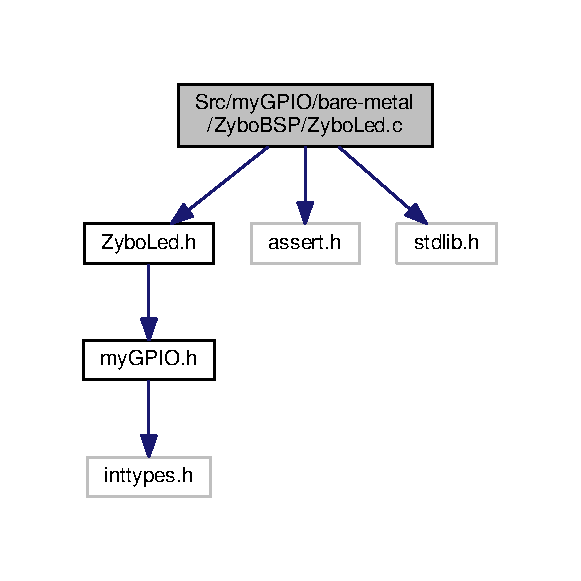
\includegraphics[width=279pt]{_zybo_led_8c__incl}
\end{center}
\end{figure}
\subsection*{Funzioni}
\begin{DoxyCompactItemize}
\item 
static int \hyperlink{_zybo_led_8c_a2a3452033228e251b3897e89a8ebcc7e}{validate\+Pair} (\hyperlink{struct_zybo_led__t}{Zybo\+Led\+\_\+t} $\ast$leds)
\item 
void \hyperlink{group___led_ga51bccd37e6ae8cd32e2c50c60a5e83cc}{Zybo\+Led\+\_\+init} (\hyperlink{struct_zybo_led__t}{Zybo\+Led\+\_\+t} $\ast$leds, \hyperlink{structmy_g_p_i_o__t}{my\+G\+P\+I\+O\+\_\+t} $\ast$gpio, \hyperlink{group__my_g_p_i_o_ga402a0d20afc0cb7c25554b8b023f4253}{my\+G\+P\+I\+O\+\_\+mask} Led3\+\_\+pin, \hyperlink{group__my_g_p_i_o_ga402a0d20afc0cb7c25554b8b023f4253}{my\+G\+P\+I\+O\+\_\+mask} Led2\+\_\+pin, \hyperlink{group__my_g_p_i_o_ga402a0d20afc0cb7c25554b8b023f4253}{my\+G\+P\+I\+O\+\_\+mask} Led1\+\_\+pin, \hyperlink{group__my_g_p_i_o_ga402a0d20afc0cb7c25554b8b023f4253}{my\+G\+P\+I\+O\+\_\+mask} Led0\+\_\+pin)
\begin{DoxyCompactList}\small\item\em Inizializza un oggetto di tipo \hyperlink{struct_zybo_led__t}{Zybo\+Led\+\_\+t}. \end{DoxyCompactList}\item 
void \hyperlink{group___led_gacf5c2b0328c4bdf2d796397fc4510c69}{Zybo\+Led\+\_\+set\+Status} (\hyperlink{struct_zybo_led__t}{Zybo\+Led\+\_\+t} $\ast$leds, \hyperlink{group___led_gad11701cccac394f7e1f90de8f85695f3}{Zybo\+Led\+\_\+mask\+\_\+t} mask, \hyperlink{group___led_ga3dcb274f22e577705c49944b8d1f4b12}{Zybo\+Led\+\_\+status\+\_\+t} status)
\begin{DoxyCompactList}\small\item\em Permette di accendere/spegnere i Led sulla board. \end{DoxyCompactList}\item 
void \hyperlink{group___led_ga20ddd78a98b4c0123c5b964aa0a59046}{Zybo\+Led\+\_\+toggle} (\hyperlink{struct_zybo_led__t}{Zybo\+Led\+\_\+t} $\ast$leds, \hyperlink{group___led_gad11701cccac394f7e1f90de8f85695f3}{Zybo\+Led\+\_\+mask\+\_\+t} mask)
\begin{DoxyCompactList}\small\item\em Permette di accendere/spegnere i Led sulla board, invertendone il valore. \end{DoxyCompactList}\end{DoxyCompactItemize}


\subsection{Descrizione dettagliata}
\begin{DoxyAuthor}{Autore}
Salvatore Barone \href{mailto:salvator.barone@gmail.com}{\tt salvator.\+barone@gmail.\+com}
\end{DoxyAuthor}
\begin{DoxyCopyright}{Copyright}
Copyright 2017 Salvatore Barone \href{mailto:salvator.barone@gmail.com}{\tt salvator.\+barone@gmail.\+com}
\end{DoxyCopyright}
This file is part of Zynq7000\+Driver\+Pack

Zynq7000\+Driver\+Pack is free software; you can redistribute it and/or modify it under the terms of the G\+N\+U General Public License as published by the Free Software Foundation; either version 3 of the License, or any later version.

Zynq7000\+Driver\+Pack is distributed in the hope that it will be useful, but W\+I\+T\+H\+O\+U\+T A\+N\+Y W\+A\+R\+R\+A\+N\+T\+Y; without even the implied warranty of M\+E\+R\+C\+H\+A\+N\+T\+A\+B\+I\+L\+I\+T\+Y or F\+I\+T\+N\+E\+S\+S F\+O\+R A P\+A\+R\+T\+I\+C\+U\+L\+A\+R P\+U\+R\+P\+O\+S\+E. See the G\+N\+U General Public License for more details.

You should have received a copy of the G\+N\+U General Public License along with this program; if not, write to the Free Software Foundation, Inc., 51 Franklin Street, Fifth Floor, Boston, M\+A 02110-\/1301, U\+S\+A. 

\subsection{Documentazione delle funzioni}
\hypertarget{_zybo_led_8c_a2a3452033228e251b3897e89a8ebcc7e}{\index{Zybo\+Led.\+c@{Zybo\+Led.\+c}!validate\+Pair@{validate\+Pair}}
\index{validate\+Pair@{validate\+Pair}!Zybo\+Led.\+c@{Zybo\+Led.\+c}}
\subsubsection[{validate\+Pair}]{\setlength{\rightskip}{0pt plus 5cm}static int validate\+Pair (
\begin{DoxyParamCaption}
\item[{{\bf Zybo\+Led\+\_\+t} $\ast$}]{leds}
\end{DoxyParamCaption}
)\hspace{0.3cm}{\ttfamily [static]}}}\label{_zybo_led_8c_a2a3452033228e251b3897e89a8ebcc7e}

\hypertarget{_zybo_led_8h}{\section{Riferimenti per il file Zybo/\+Zybo\+Led.h}
\label{_zybo_led_8h}\index{Zybo/\+Zybo\+Led.\+h@{Zybo/\+Zybo\+Led.\+h}}
}
{\ttfamily \#include \char`\"{}my\+G\+P\+I\+O.\+h\char`\"{}}\\*
Grafo delle dipendenze di inclusione per Zybo\+Led.\+h\+:\nopagebreak
\begin{figure}[H]
\begin{center}
\leavevmode
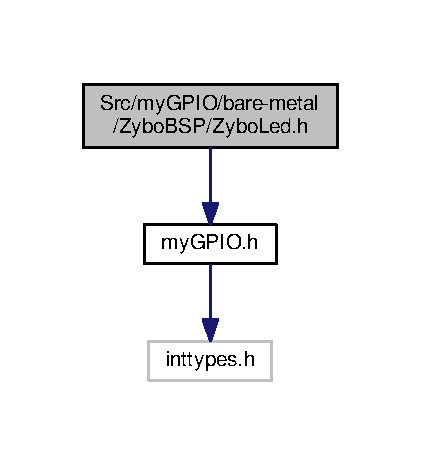
\includegraphics[width=167pt]{_zybo_led_8h__incl}
\end{center}
\end{figure}
Questo grafo mostra quali altri file includono direttamente o indirettamente questo file\+:\nopagebreak
\begin{figure}[H]
\begin{center}
\leavevmode
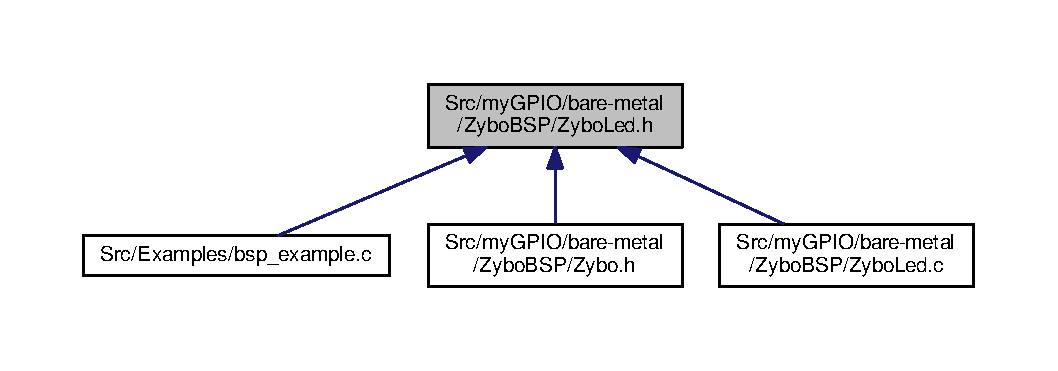
\includegraphics[width=256pt]{_zybo_led_8h__dep__incl}
\end{center}
\end{figure}
\subsection*{Strutture dati}
\begin{DoxyCompactItemize}
\item 
struct \hyperlink{struct_zybo_led__t}{Zybo\+Led\+\_\+t}
\begin{DoxyCompactList}\small\item\em Struttura opaca che astrae l'insieme dei Led presenti sulla board Digilent Zybo;. \end{DoxyCompactList}\end{DoxyCompactItemize}
\subsection*{Definizioni}
\begin{DoxyCompactItemize}
\item 
\#define \hyperlink{group___led_ga50ab39fed34dc3aaf53cdfd67d8ba25d}{Zybo\+Led}(i)~((uint32\+\_\+t)(1$<$$<$(i)))
\begin{DoxyCompactList}\small\item\em Metodo alternativo per la specifica di uno dei led presenti sulla board Digilent Zybo. \end{DoxyCompactList}\end{DoxyCompactItemize}
\subsection*{Tipi enumerati (enum)}
\begin{DoxyCompactItemize}
\item 
enum \hyperlink{group___led_gad11701cccac394f7e1f90de8f85695f3}{Zybo\+Led\+\_\+mask\+\_\+t} \{ \hyperlink{group___led_ggad11701cccac394f7e1f90de8f85695f3adc5edc2adfd899da9f149cb61364b141}{Zybo\+Led3} = 0x8\+U, 
\hyperlink{group___led_ggad11701cccac394f7e1f90de8f85695f3a4fa521f6fce7c4ba77d1d8144e71cdfc}{Zybo\+Led2} = 0x4\+U, 
\hyperlink{group___led_ggad11701cccac394f7e1f90de8f85695f3ad71c06f65dfffcf825d48f287718d9be}{Zybo\+Led1} = 0x2\+U, 
\hyperlink{group___led_ggad11701cccac394f7e1f90de8f85695f3ae1a1e8fa0bf803793ff27004884b85fe}{Zybo\+Led0} = 0x1\+U
 \}
\begin{DoxyCompactList}\small\item\em Maschere di selezione dei led. \end{DoxyCompactList}\item 
enum \hyperlink{group___led_ga3dcb274f22e577705c49944b8d1f4b12}{Zybo\+Led\+\_\+status\+\_\+t} \{ \hyperlink{group___led_gga3dcb274f22e577705c49944b8d1f4b12a9679f1c302afdb51915a2331b4ec92f3}{Zybo\+Led\+\_\+off}, 
\hyperlink{group___led_gga3dcb274f22e577705c49944b8d1f4b12aafcf0ae16a6edec807c06bb0a99f7e8b}{Zybo\+Led\+\_\+on}
 \}
\begin{DoxyCompactList}\small\item\em Status di accensione/spegnimento dei led. \end{DoxyCompactList}\end{DoxyCompactItemize}
\subsection*{Funzioni}
\begin{DoxyCompactItemize}
\item 
void \hyperlink{group___led_ga51bccd37e6ae8cd32e2c50c60a5e83cc}{Zybo\+Led\+\_\+init} (\hyperlink{struct_zybo_led__t}{Zybo\+Led\+\_\+t} $\ast$leds, \hyperlink{structmy_g_p_i_o__t}{my\+G\+P\+I\+O\+\_\+t} $\ast$gpio, \hyperlink{group__my_g_p_i_o_ga402a0d20afc0cb7c25554b8b023f4253}{my\+G\+P\+I\+O\+\_\+mask} Led3\+\_\+pin, \hyperlink{group__my_g_p_i_o_ga402a0d20afc0cb7c25554b8b023f4253}{my\+G\+P\+I\+O\+\_\+mask} Led2\+\_\+pin, \hyperlink{group__my_g_p_i_o_ga402a0d20afc0cb7c25554b8b023f4253}{my\+G\+P\+I\+O\+\_\+mask} Led1\+\_\+pin, \hyperlink{group__my_g_p_i_o_ga402a0d20afc0cb7c25554b8b023f4253}{my\+G\+P\+I\+O\+\_\+mask} Led0\+\_\+pin)
\begin{DoxyCompactList}\small\item\em Inizializza un oggetto di tipo \hyperlink{struct_zybo_led__t}{Zybo\+Led\+\_\+t}. \end{DoxyCompactList}\item 
void \hyperlink{group___led_gacf5c2b0328c4bdf2d796397fc4510c69}{Zybo\+Led\+\_\+set\+Status} (\hyperlink{struct_zybo_led__t}{Zybo\+Led\+\_\+t} $\ast$leds, \hyperlink{group___led_gad11701cccac394f7e1f90de8f85695f3}{Zybo\+Led\+\_\+mask\+\_\+t} mask, \hyperlink{group___led_ga3dcb274f22e577705c49944b8d1f4b12}{Zybo\+Led\+\_\+status\+\_\+t} status)
\begin{DoxyCompactList}\small\item\em Permette di accendere/spegnere i Led sulla board. \end{DoxyCompactList}\item 
void \hyperlink{group___led_ga20ddd78a98b4c0123c5b964aa0a59046}{Zybo\+Led\+\_\+toggle} (\hyperlink{struct_zybo_led__t}{Zybo\+Led\+\_\+t} $\ast$leds, \hyperlink{group___led_gad11701cccac394f7e1f90de8f85695f3}{Zybo\+Led\+\_\+mask\+\_\+t} mask)
\begin{DoxyCompactList}\small\item\em Permette di accendere/spegnere i Led sulla board, invertendone il valore. \end{DoxyCompactList}\end{DoxyCompactItemize}


\subsection{Descrizione dettagliata}
\begin{DoxyAuthor}{Autore}
Salvatore Barone \href{mailto:salvator.barone@gmail.com}{\tt salvator.\+barone@gmail.\+com}
\end{DoxyAuthor}
\begin{DoxyCopyright}{Copyright}
Copyright 2017 Salvatore Barone \href{mailto:salvator.barone@gmail.com}{\tt salvator.\+barone@gmail.\+com}
\end{DoxyCopyright}
This file is part of Zynq7000\+Driver\+Pack

Zynq7000\+Driver\+Pack is free software; you can redistribute it and/or modify it under the terms of the G\+N\+U General Public License as published by the Free Software Foundation; either version 3 of the License, or any later version.

Zynq7000\+Driver\+Pack is distributed in the hope that it will be useful, but W\+I\+T\+H\+O\+U\+T A\+N\+Y W\+A\+R\+R\+A\+N\+T\+Y; without even the implied warranty of M\+E\+R\+C\+H\+A\+N\+T\+A\+B\+I\+L\+I\+T\+Y or F\+I\+T\+N\+E\+S\+S F\+O\+R A P\+A\+R\+T\+I\+C\+U\+L\+A\+R P\+U\+R\+P\+O\+S\+E. See the G\+N\+U General Public License for more details.

You should have received a copy of the G\+N\+U General Public License along with this program; if not, write to the Free Software Foundation, Inc., 51 Franklin Street, Fifth Floor, Boston, M\+A 02110-\/1301, U\+S\+A. 
\hypertarget{_zybo_switch_8c}{\section{Riferimenti per il file Zybo/\+Zybo\+Switch.c}
\label{_zybo_switch_8c}\index{Zybo/\+Zybo\+Switch.\+c@{Zybo/\+Zybo\+Switch.\+c}}
}
{\ttfamily \#include \char`\"{}Zybo\+Switch.\+h\char`\"{}}\\*
{\ttfamily \#include $<$assert.\+h$>$}\\*
{\ttfamily \#include $<$stdlib.\+h$>$}\\*
Grafo delle dipendenze di inclusione per Zybo\+Switch.\+c\+:\nopagebreak
\begin{figure}[H]
\begin{center}
\leavevmode
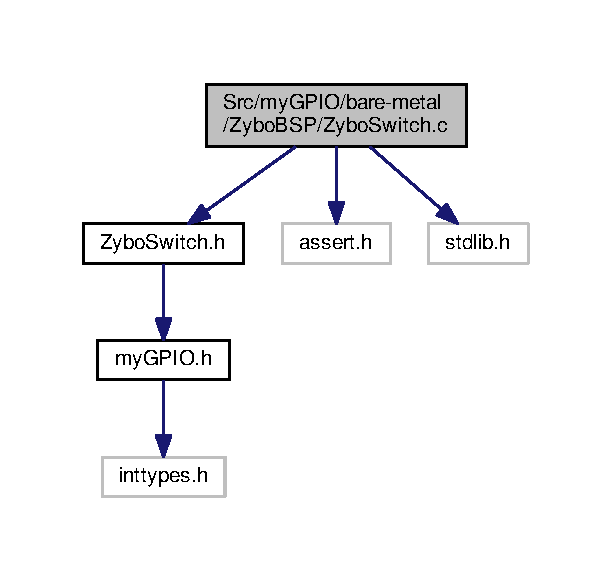
\includegraphics[width=294pt]{_zybo_switch_8c__incl}
\end{center}
\end{figure}
\subsection*{Funzioni}
\begin{DoxyCompactItemize}
\item 
void \hyperlink{group___switch_ga121018c0ccfeb05b6e8f692a5a6955d7}{Zybo\+Switch\+\_\+init} (\hyperlink{struct_zybo_switch__t}{Zybo\+Switch\+\_\+t} $\ast$switches, \hyperlink{struct_g_p_i_o__t}{G\+P\+I\+O\+\_\+t} $\ast$gpio, \hyperlink{group___g_p_i_o_ga6d5aef8a8a54ee2f602d47252ff66595}{G\+P\+I\+O\+\_\+mask} Switch3\+\_\+pin, \hyperlink{group___g_p_i_o_ga6d5aef8a8a54ee2f602d47252ff66595}{G\+P\+I\+O\+\_\+mask} Switch2\+\_\+pin, \hyperlink{group___g_p_i_o_ga6d5aef8a8a54ee2f602d47252ff66595}{G\+P\+I\+O\+\_\+mask} Switch1\+\_\+pin, \hyperlink{group___g_p_i_o_ga6d5aef8a8a54ee2f602d47252ff66595}{G\+P\+I\+O\+\_\+mask} Switch0\+\_\+pin)
\begin{DoxyCompactList}\small\item\em Inizializza un oggetto di tipo \hyperlink{struct_zybo_switch__t}{Zybo\+Switch\+\_\+t}. \end{DoxyCompactList}\item 
\hyperlink{group___switch_ga4ba6b49b2f47ebb464aefcea7e23e04a}{Zybo\+Switch\+\_\+status\+\_\+t} \hyperlink{group___switch_gafac8daf9a9a585f8f20ef2a6fa883a1f}{Zybo\+Switch\+\_\+get\+Status} (\hyperlink{struct_zybo_switch__t}{Zybo\+Switch\+\_\+t} $\ast$switches, \hyperlink{group___switch_ga2e0602a824354f25c395f938caba3703}{Zybo\+Switch\+\_\+mask\+\_\+t} mask)
\begin{DoxyCompactList}\small\item\em Permette la lettura dello stato degli switch presenti sulla board. \end{DoxyCompactList}\end{DoxyCompactItemize}

\hypertarget{_zybo_switch_8h}{\section{Riferimenti per il file Zybo/\+Zybo\+Switch.h}
\label{_zybo_switch_8h}\index{Zybo/\+Zybo\+Switch.\+h@{Zybo/\+Zybo\+Switch.\+h}}
}
{\ttfamily \#include \char`\"{}gpio.\+h\char`\"{}}\\*
Grafo delle dipendenze di inclusione per Zybo\+Switch.\+h\+:
\nopagebreak
\begin{figure}[H]
\begin{center}
\leavevmode
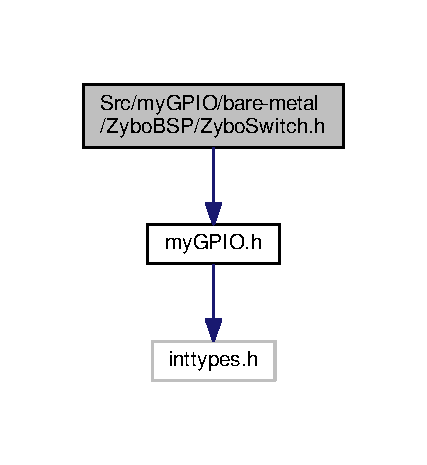
\includegraphics[width=181pt]{_zybo_switch_8h__incl}
\end{center}
\end{figure}
Questo grafo mostra quali altri file includono direttamente o indirettamente questo file\+:
\nopagebreak
\begin{figure}[H]
\begin{center}
\leavevmode
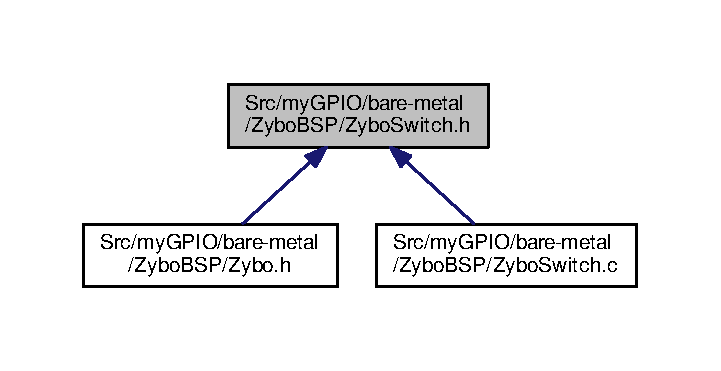
\includegraphics[width=270pt]{_zybo_switch_8h__dep__incl}
\end{center}
\end{figure}
\subsection*{Strutture dati}
\begin{DoxyCompactItemize}
\item 
struct \hyperlink{struct_zybo_switch__t}{Zybo\+Switch\+\_\+t}
\begin{DoxyCompactList}\small\item\em Struttura opaca che astrae l'insieme degli switch presenti sulla board Digilent Zybo;. \end{DoxyCompactList}\end{DoxyCompactItemize}
\subsection*{Definizioni}
\begin{DoxyCompactItemize}
\item 
\#define \hyperlink{group___switch_ga1c463f6e1e3a43f68109c176772ce5cc}{Zybo\+Switch}(i)~((uint32\+\_\+t)(1$<$$<$i))
\begin{DoxyCompactList}\small\item\em Metodo alternativo per la specifica di uno degli switch presenti sulla board Digilent Zybo. \end{DoxyCompactList}\end{DoxyCompactItemize}
\subsection*{Tipi enumerati (enum)}
\begin{DoxyCompactItemize}
\item 
enum \hyperlink{group___switch_ga2e0602a824354f25c395f938caba3703}{Zybo\+Switch\+\_\+mask\+\_\+t} \{ \hyperlink{group___switch_gga2e0602a824354f25c395f938caba3703a73ccea5ad8c919fe962e9a67a3733ee3}{Zybo\+Switch3} = 0x8\+U, 
\hyperlink{group___switch_gga2e0602a824354f25c395f938caba3703aac2f5ebb28eb3bd93fcdf8019b6a3e9e}{Zybo\+Switch2} = 0x4\+U, 
\hyperlink{group___switch_gga2e0602a824354f25c395f938caba3703a694a25c87b1ec597d2a6032bf5d34b0f}{Zybo\+Switch1} = 0x2\+U, 
\hyperlink{group___switch_gga2e0602a824354f25c395f938caba3703a84350e8b6e7a7e2cabf22fc7a1a5c651}{Zybo\+Switch0} = 0x1\+U
 \}
\begin{DoxyCompactList}\small\item\em Maschere di selezione degli switch. \end{DoxyCompactList}\item 
enum \hyperlink{group___switch_ga4ba6b49b2f47ebb464aefcea7e23e04a}{Zybo\+Switch\+\_\+status\+\_\+t} \{ \hyperlink{group___switch_gga4ba6b49b2f47ebb464aefcea7e23e04aa1d686faf83e8606e68eec0b7e525a755}{Zybo\+Switch\+\_\+off}, 
\hyperlink{group___switch_gga4ba6b49b2f47ebb464aefcea7e23e04aafba009508b8822de867af69034e3e4f8}{Zybo\+Switch\+\_\+on}
 \}
\begin{DoxyCompactList}\small\item\em Status di attivo/inattivo degli switch. \end{DoxyCompactList}\end{DoxyCompactItemize}
\subsection*{Funzioni}
\begin{DoxyCompactItemize}
\item 
void \hyperlink{group___switch_ga121018c0ccfeb05b6e8f692a5a6955d7}{Zybo\+Switch\+\_\+init} (\hyperlink{struct_zybo_switch__t}{Zybo\+Switch\+\_\+t} $\ast$switches, G\+P\+I\+O\+\_\+t $\ast$gpio, G\+P\+I\+O\+\_\+mask Switch3\+\_\+pin, G\+P\+I\+O\+\_\+mask Switch2\+\_\+pin, G\+P\+I\+O\+\_\+mask Switch1\+\_\+pin, G\+P\+I\+O\+\_\+mask Switch0\+\_\+pin)
\begin{DoxyCompactList}\small\item\em Inizializza un oggetto di tipo \hyperlink{struct_zybo_switch__t}{Zybo\+Switch\+\_\+t}. \end{DoxyCompactList}\item 
\hyperlink{group___switch_ga4ba6b49b2f47ebb464aefcea7e23e04a}{Zybo\+Switch\+\_\+status\+\_\+t} \hyperlink{group___switch_gafac8daf9a9a585f8f20ef2a6fa883a1f}{Zybo\+Switch\+\_\+get\+Status} (\hyperlink{struct_zybo_switch__t}{Zybo\+Switch\+\_\+t} $\ast$switches, \hyperlink{group___switch_ga2e0602a824354f25c395f938caba3703}{Zybo\+Switch\+\_\+mask\+\_\+t} mask)
\begin{DoxyCompactList}\small\item\em Permette la lettura dello stato degli switch presenti sulla board. \end{DoxyCompactList}\end{DoxyCompactItemize}

\hypertarget{my_g_p_i_o_k__list_8c}{\section{Riferimenti per il file Src/my\+G\+P\+I\+O/linux-\/driver/my\+G\+P\+I\+O\+K\+\_\+list.c}
\label{my_g_p_i_o_k__list_8c}\index{Src/my\+G\+P\+I\+O/linux-\/driver/my\+G\+P\+I\+O\+K\+\_\+list.\+c@{Src/my\+G\+P\+I\+O/linux-\/driver/my\+G\+P\+I\+O\+K\+\_\+list.\+c}}
}
{\ttfamily \#include \char`\"{}my\+G\+P\+I\+O\+K\+\_\+list.\+h\char`\"{}}\\*
{\ttfamily \#include $<$linux/slab.\+h$>$}\\*
Grafo delle dipendenze di inclusione per my\+G\+P\+I\+O\+K\+\_\+list.\+c\+:
\nopagebreak
\begin{figure}[H]
\begin{center}
\leavevmode
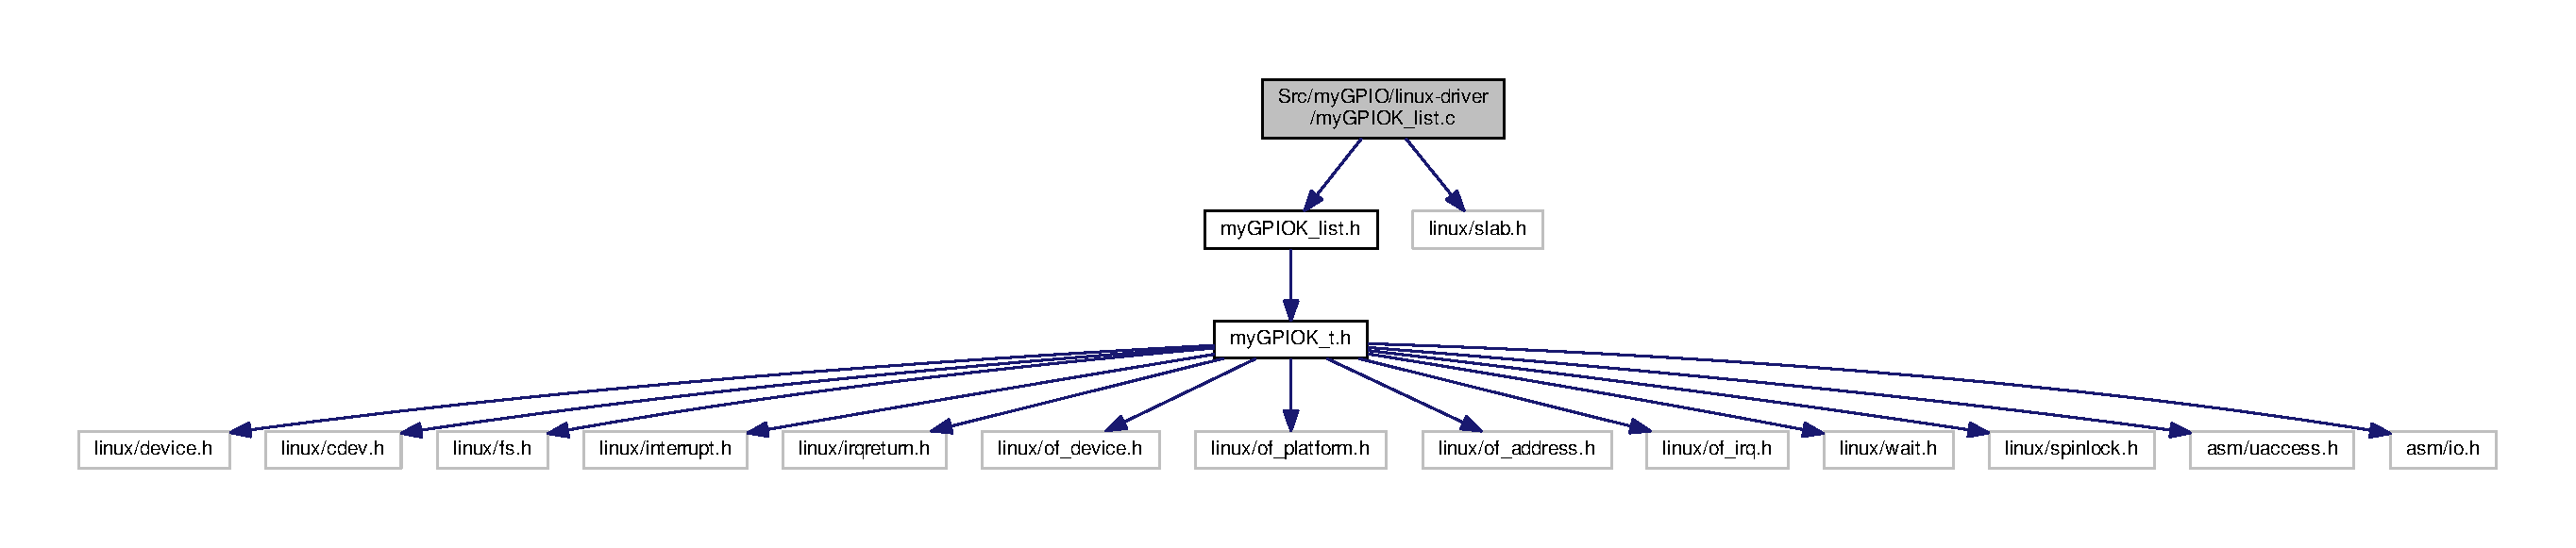
\includegraphics[width=350pt]{my_g_p_i_o_k__list_8c__incl}
\end{center}
\end{figure}
\subsection*{Funzioni}
\begin{DoxyCompactItemize}
\item 
int \hyperlink{group___device_list_ga1051095fc78c8ba7cf0b20a20fa253d2}{my\+G\+P\+I\+O\+K\+\_\+list\+\_\+\+Init} (\hyperlink{structmy_g_p_i_o_k__list__t}{my\+G\+P\+I\+O\+K\+\_\+list\+\_\+t} $\ast$list, uint32\+\_\+t list\+\_\+size)
\begin{DoxyCompactList}\small\item\em Inizializza una struttura dati \hyperlink{structmy_g_p_i_o_k__list__t}{my\+G\+P\+I\+O\+K\+\_\+list\+\_\+t}. \end{DoxyCompactList}\item 
void \hyperlink{group___device_list_ga416dfff8f4bf6034c87d60968056c621}{my\+G\+P\+I\+O\+K\+\_\+list\+\_\+\+Destroy} (\hyperlink{structmy_g_p_i_o_k__list__t}{my\+G\+P\+I\+O\+K\+\_\+list\+\_\+t} $\ast$list)
\begin{DoxyCompactList}\small\item\em Dealloca gli oggetti internamente gestiti da un oggetto \hyperlink{structmy_g_p_i_o_k__list__t}{my\+G\+P\+I\+O\+K\+\_\+list\+\_\+t}, liberando la memoria. \end{DoxyCompactList}\item 
int \hyperlink{group___device_list_gac5048cf2dbbbce3c39485e15595e88c9}{my\+G\+P\+I\+O\+K\+\_\+list\+\_\+add} (\hyperlink{structmy_g_p_i_o_k__list__t}{my\+G\+P\+I\+O\+K\+\_\+list\+\_\+t} $\ast$list, \hyperlink{structmy_g_p_i_o_k__t}{my\+G\+P\+I\+O\+K\+\_\+t} $\ast$device)
\begin{DoxyCompactList}\small\item\em Aggiunge un riferimento ad un oggetto \hyperlink{structmy_g_p_i_o_k__t}{my\+G\+P\+I\+O\+K\+\_\+t} alla lista. \end{DoxyCompactList}\item 
\hyperlink{structmy_g_p_i_o_k__t}{my\+G\+P\+I\+O\+K\+\_\+t} $\ast$ \hyperlink{group___device_list_ga616aa45c32b2ff391fc2b89930d1141b}{my\+G\+P\+I\+O\+K\+\_\+list\+\_\+find\+\_\+by\+\_\+op} (\hyperlink{structmy_g_p_i_o_k__list__t}{my\+G\+P\+I\+O\+K\+\_\+list\+\_\+t} $\ast$list, struct platform\+\_\+device $\ast$op)
\begin{DoxyCompactList}\small\item\em Ricerca un oggetto \hyperlink{structmy_g_p_i_o_k__t}{my\+G\+P\+I\+O\+K\+\_\+t} all'interno della lista. \end{DoxyCompactList}\item 
\hyperlink{structmy_g_p_i_o_k__t}{my\+G\+P\+I\+O\+K\+\_\+t} $\ast$ \hyperlink{group___device_list_gaf50b0da291040e8da5050194a4979849}{my\+G\+P\+I\+O\+K\+\_\+list\+\_\+find\+\_\+by\+\_\+minor} (\hyperlink{structmy_g_p_i_o_k__list__t}{my\+G\+P\+I\+O\+K\+\_\+list\+\_\+t} $\ast$list, dev\+\_\+t dev)
\begin{DoxyCompactList}\small\item\em Ricerca un oggetto \hyperlink{structmy_g_p_i_o_k__t}{my\+G\+P\+I\+O\+K\+\_\+t} all'interno della lista. \end{DoxyCompactList}\item 
\hyperlink{structmy_g_p_i_o_k__t}{my\+G\+P\+I\+O\+K\+\_\+t} $\ast$ \hyperlink{group___device_list_ga0bb70e18f51367d95fa28f723679ac30}{my\+G\+P\+I\+O\+K\+\_\+list\+\_\+find\+\_\+irq\+\_\+line} (\hyperlink{structmy_g_p_i_o_k__list__t}{my\+G\+P\+I\+O\+K\+\_\+list\+\_\+t} $\ast$list, int irq\+\_\+line)
\begin{DoxyCompactList}\small\item\em Ricerca un oggetto \hyperlink{structmy_g_p_i_o_k__t}{my\+G\+P\+I\+O\+K\+\_\+t} all'interno della lista. \end{DoxyCompactList}\item 
uint32\+\_\+t \hyperlink{group___device_list_ga731d5b5cbb96c6c5ef53936c23cdc58a}{my\+G\+P\+I\+O\+K\+\_\+list\+\_\+device\+\_\+count} (\hyperlink{structmy_g_p_i_o_k__list__t}{my\+G\+P\+I\+O\+K\+\_\+list\+\_\+t} $\ast$list)
\begin{DoxyCompactList}\small\item\em Restituisce il numero di device correntemente inseriti nella lista. \end{DoxyCompactList}\end{DoxyCompactItemize}


\subsection{Descrizione dettagliata}
\begin{DoxyAuthor}{Autore}
Salvatore Barone \href{mailto:salvator.barone@gmail.com}{\tt salvator.\+barone@gmail.\+com} 
\end{DoxyAuthor}
\begin{DoxyDate}{Data}
24 06 2017
\end{DoxyDate}
\begin{DoxyCopyright}{Copyright}
Copyright 2017 Salvatore Barone \href{mailto:salvator.barone@gmail.com}{\tt salvator.\+barone@gmail.\+com}
\end{DoxyCopyright}
This file is part of Zynq7000\+Driver\+Pack

Zynq7000\+Driver\+Pack is free software; you can redistribute it and/or modify it under the terms of the G\+N\+U General Public License as published by the Free Software Foundation; either version 3 of the License, or any later version.

Zynq7000\+Driver\+Pack is distributed in the hope that it will be useful, but W\+I\+T\+H\+O\+U\+T A\+N\+Y W\+A\+R\+R\+A\+N\+T\+Y; without even the implied warranty of M\+E\+R\+C\+H\+A\+N\+T\+A\+B\+I\+L\+I\+T\+Y or F\+I\+T\+N\+E\+S\+S F\+O\+R A P\+A\+R\+T\+I\+C\+U\+L\+A\+R P\+U\+R\+P\+O\+S\+E. See the G\+N\+U General Public License for more details.

You should have received a copy of the G\+N\+U General Public License along with this program; if not, write to the Free Software Foundation, Inc., 51 Franklin Street, Fifth Floor, Boston, M\+A 02110-\/1301, U\+S\+A. 
\hypertarget{my_g_p_i_o_k__list_8h}{}\section{Riferimenti per il file Src/my\+G\+P\+I\+O/linux-\/driver/my\+G\+P\+I\+O\+K\+\_\+list.h}
\label{my_g_p_i_o_k__list_8h}\index{Src/my\+G\+P\+I\+O/linux-\/driver/my\+G\+P\+I\+O\+K\+\_\+list.\+h@{Src/my\+G\+P\+I\+O/linux-\/driver/my\+G\+P\+I\+O\+K\+\_\+list.\+h}}
{\ttfamily \#include \char`\"{}my\+G\+P\+I\+O\+K\+\_\+t.\+h\char`\"{}}\newline
Grafo delle dipendenze di inclusione per my\+G\+P\+I\+O\+K\+\_\+list.\+h\+:\nopagebreak
\begin{figure}[H]
\begin{center}
\leavevmode
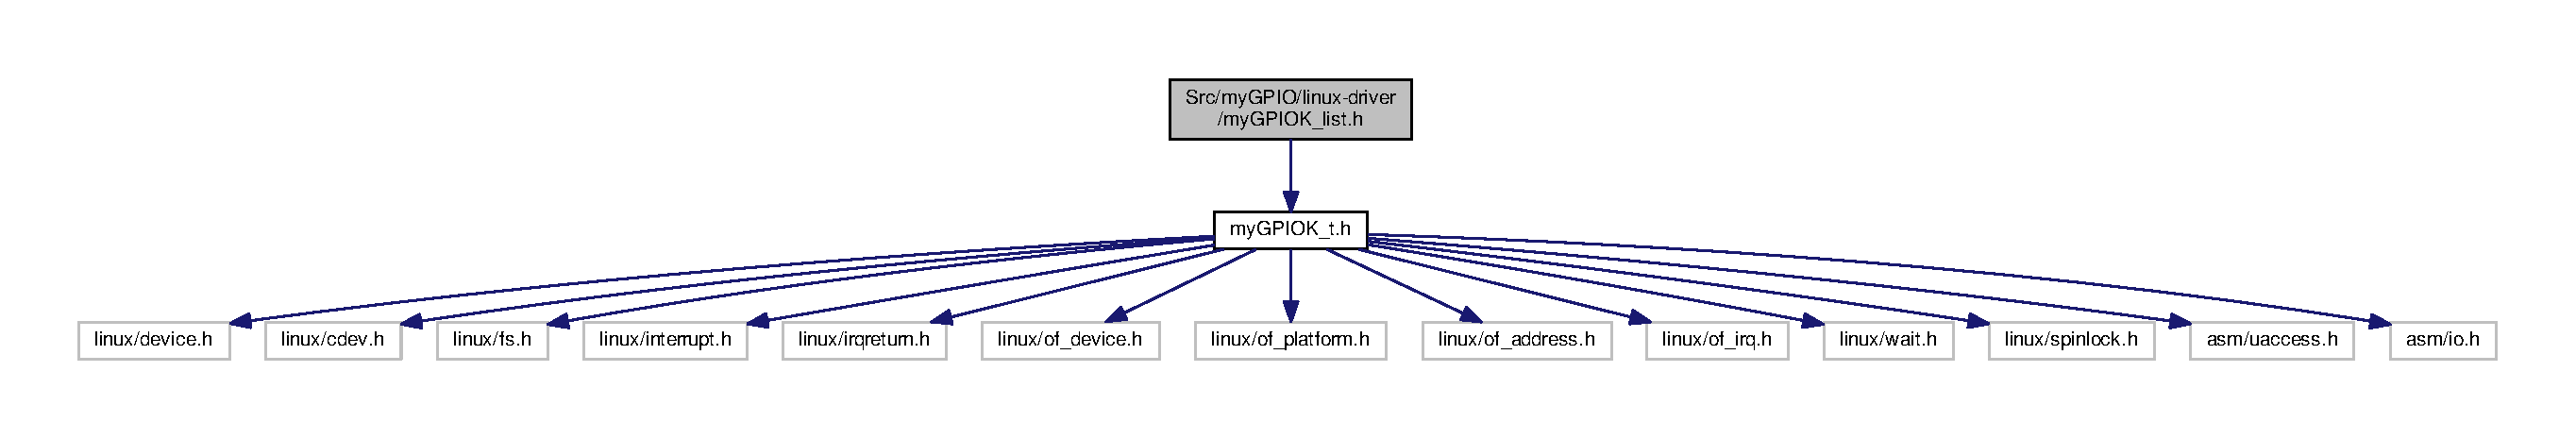
\includegraphics[width=350pt]{my_g_p_i_o_k__list_8h__incl}
\end{center}
\end{figure}
Questo grafo mostra quali altri file includono direttamente o indirettamente questo file\+:\nopagebreak
\begin{figure}[H]
\begin{center}
\leavevmode
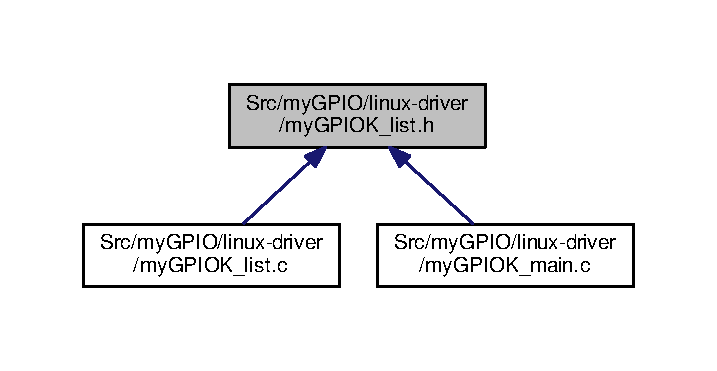
\includegraphics[width=344pt]{my_g_p_i_o_k__list_8h__dep__incl}
\end{center}
\end{figure}
\subsection*{Strutture dati}
\begin{DoxyCompactItemize}
\item 
struct \hyperlink{structmy_g_p_i_o_k__list__t}{my\+G\+P\+I\+O\+K\+\_\+list\+\_\+t}
\begin{DoxyCompactList}\small\item\em Struttura dati per la gestione degli oggetti \hyperlink{structmy_g_p_i_o_k__t}{my\+G\+P\+I\+O\+K\+\_\+t} gestiti dal driver. \end{DoxyCompactList}\end{DoxyCompactItemize}
\subsection*{Funzioni}
\begin{DoxyCompactItemize}
\item 
int \hyperlink{group___device_list_ga1051095fc78c8ba7cf0b20a20fa253d2}{my\+G\+P\+I\+O\+K\+\_\+list\+\_\+\+Init} (\hyperlink{structmy_g_p_i_o_k__list__t}{my\+G\+P\+I\+O\+K\+\_\+list\+\_\+t} $\ast$list, uint32\+\_\+t list\+\_\+size)
\begin{DoxyCompactList}\small\item\em Inizializza una struttura dati \hyperlink{structmy_g_p_i_o_k__list__t}{my\+G\+P\+I\+O\+K\+\_\+list\+\_\+t}. \end{DoxyCompactList}\item 
void \hyperlink{group___device_list_ga416dfff8f4bf6034c87d60968056c621}{my\+G\+P\+I\+O\+K\+\_\+list\+\_\+\+Destroy} (\hyperlink{structmy_g_p_i_o_k__list__t}{my\+G\+P\+I\+O\+K\+\_\+list\+\_\+t} $\ast$list)
\begin{DoxyCompactList}\small\item\em Dealloca gli oggetti internamente gestiti da un oggetto \hyperlink{structmy_g_p_i_o_k__list__t}{my\+G\+P\+I\+O\+K\+\_\+list\+\_\+t}, liberando la memoria. \end{DoxyCompactList}\item 
int \hyperlink{group___device_list_gac5048cf2dbbbce3c39485e15595e88c9}{my\+G\+P\+I\+O\+K\+\_\+list\+\_\+add} (\hyperlink{structmy_g_p_i_o_k__list__t}{my\+G\+P\+I\+O\+K\+\_\+list\+\_\+t} $\ast$list, \hyperlink{structmy_g_p_i_o_k__t}{my\+G\+P\+I\+O\+K\+\_\+t} $\ast$device)
\begin{DoxyCompactList}\small\item\em Aggiunge un riferimento ad un oggetto \hyperlink{structmy_g_p_i_o_k__t}{my\+G\+P\+I\+O\+K\+\_\+t} alla lista. \end{DoxyCompactList}\item 
\hyperlink{structmy_g_p_i_o_k__t}{my\+G\+P\+I\+O\+K\+\_\+t} $\ast$ \hyperlink{group___device_list_ga616aa45c32b2ff391fc2b89930d1141b}{my\+G\+P\+I\+O\+K\+\_\+list\+\_\+find\+\_\+by\+\_\+op} (\hyperlink{structmy_g_p_i_o_k__list__t}{my\+G\+P\+I\+O\+K\+\_\+list\+\_\+t} $\ast$list, struct platform\+\_\+device $\ast$op)
\begin{DoxyCompactList}\small\item\em Ricerca un oggetto \hyperlink{structmy_g_p_i_o_k__t}{my\+G\+P\+I\+O\+K\+\_\+t} all\textquotesingle{}interno della lista. \end{DoxyCompactList}\item 
\hyperlink{structmy_g_p_i_o_k__t}{my\+G\+P\+I\+O\+K\+\_\+t} $\ast$ \hyperlink{group___device_list_gaf50b0da291040e8da5050194a4979849}{my\+G\+P\+I\+O\+K\+\_\+list\+\_\+find\+\_\+by\+\_\+minor} (\hyperlink{structmy_g_p_i_o_k__list__t}{my\+G\+P\+I\+O\+K\+\_\+list\+\_\+t} $\ast$list, dev\+\_\+t dev)
\begin{DoxyCompactList}\small\item\em Ricerca un oggetto \hyperlink{structmy_g_p_i_o_k__t}{my\+G\+P\+I\+O\+K\+\_\+t} all\textquotesingle{}interno della lista. \end{DoxyCompactList}\item 
\hyperlink{structmy_g_p_i_o_k__t}{my\+G\+P\+I\+O\+K\+\_\+t} $\ast$ \hyperlink{group___device_list_ga0bb70e18f51367d95fa28f723679ac30}{my\+G\+P\+I\+O\+K\+\_\+list\+\_\+find\+\_\+irq\+\_\+line} (\hyperlink{structmy_g_p_i_o_k__list__t}{my\+G\+P\+I\+O\+K\+\_\+list\+\_\+t} $\ast$list, int irq\+\_\+line)
\begin{DoxyCompactList}\small\item\em Ricerca un oggetto \hyperlink{structmy_g_p_i_o_k__t}{my\+G\+P\+I\+O\+K\+\_\+t} all\textquotesingle{}interno della lista. \end{DoxyCompactList}\item 
uint32\+\_\+t \hyperlink{group___device_list_ga731d5b5cbb96c6c5ef53936c23cdc58a}{my\+G\+P\+I\+O\+K\+\_\+list\+\_\+device\+\_\+count} (\hyperlink{structmy_g_p_i_o_k__list__t}{my\+G\+P\+I\+O\+K\+\_\+list\+\_\+t} $\ast$list)
\begin{DoxyCompactList}\small\item\em Restituisce il numero di device correntemente inseriti nella lista. \end{DoxyCompactList}\end{DoxyCompactItemize}


\subsection{Descrizione dettagliata}
\begin{DoxyAuthor}{Autore}
Salvatore Barone \href{mailto:salvator.barone@gmail.com}{\tt salvator.\+barone@gmail.\+com} 
\end{DoxyAuthor}
\begin{DoxyDate}{Data}
24 06 2017
\end{DoxyDate}
\begin{DoxyCopyright}{Copyright}
Copyright 2017 Salvatore Barone \href{mailto:salvator.barone@gmail.com}{\tt salvator.\+barone@gmail.\+com}
\end{DoxyCopyright}
This file is part of Zynq7000\+Driver\+Pack

Zynq7000\+Driver\+Pack is free software; you can redistribute it and/or modify it under the terms of the G\+NU General Public License as published by the Free Software Foundation; either version 3 of the License, or any later version.

Zynq7000\+Driver\+Pack is distributed in the hope that it will be useful, but W\+I\+T\+H\+O\+UT A\+NY W\+A\+R\+R\+A\+N\+TY; without even the implied warranty of M\+E\+R\+C\+H\+A\+N\+T\+A\+B\+I\+L\+I\+TY or F\+I\+T\+N\+E\+SS F\+OR A P\+A\+R\+T\+I\+C\+U\+L\+AR P\+U\+R\+P\+O\+SE. See the G\+NU General Public License for more details.

You should have received a copy of the G\+NU General Public License along with this program; if not, write to the Free Software Foundation, Inc., 51 Franklin Street, Fifth Floor, Boston, MA 02110-\/1301, U\+SA. 
\hypertarget{my_g_p_i_o_k__main_8c}{}\section{Riferimenti per il file Src/my\+G\+P\+I\+O/linux-\/driver/my\+G\+P\+I\+O\+K\+\_\+main.c}
\label{my_g_p_i_o_k__main_8c}\index{Src/my\+G\+P\+I\+O/linux-\/driver/my\+G\+P\+I\+O\+K\+\_\+main.\+c@{Src/my\+G\+P\+I\+O/linux-\/driver/my\+G\+P\+I\+O\+K\+\_\+main.\+c}}
{\ttfamily \#include $<$linux/init.\+h$>$}\newline
{\ttfamily \#include $<$linux/module.\+h$>$}\newline
{\ttfamily \#include $<$linux/kernel.\+h$>$}\newline
{\ttfamily \#include $<$linux/slab.\+h$>$}\newline
{\ttfamily \#include $<$linux/fs.\+h$>$}\newline
{\ttfamily \#include $<$linux/errno.\+h$>$}\newline
{\ttfamily \#include $<$linux/types.\+h$>$}\newline
{\ttfamily \#include $<$linux/proc\+\_\+fs.\+h$>$}\newline
{\ttfamily \#include $<$linux/fcntl.\+h$>$}\newline
{\ttfamily \#include $<$linux/unistd.\+h$>$}\newline
{\ttfamily \#include $<$linux/platform\+\_\+device.\+h$>$}\newline
{\ttfamily \#include $<$linux/of\+\_\+device.\+h$>$}\newline
{\ttfamily \#include $<$linux/of\+\_\+platform.\+h$>$}\newline
{\ttfamily \#include $<$linux/of\+\_\+address.\+h$>$}\newline
{\ttfamily \#include $<$linux/of\+\_\+irq.\+h$>$}\newline
{\ttfamily \#include $<$linux/interrupt.\+h$>$}\newline
{\ttfamily \#include $<$linux/irqreturn.\+h$>$}\newline
{\ttfamily \#include $<$asm/uaccess.\+h$>$}\newline
{\ttfamily \#include $<$asm/io.\+h$>$}\newline
{\ttfamily \#include $<$linux/sched.\+h$>$}\newline
{\ttfamily \#include $<$linux/poll.\+h$>$}\newline
{\ttfamily \#include \char`\"{}my\+G\+P\+I\+O\+K\+\_\+t.\+h\char`\"{}}\newline
{\ttfamily \#include \char`\"{}my\+G\+P\+I\+O\+K\+\_\+list.\+h\char`\"{}}\newline
Grafo delle dipendenze di inclusione per my\+G\+P\+I\+O\+K\+\_\+main.\+c\+:\nopagebreak
\begin{figure}[H]
\begin{center}
\leavevmode
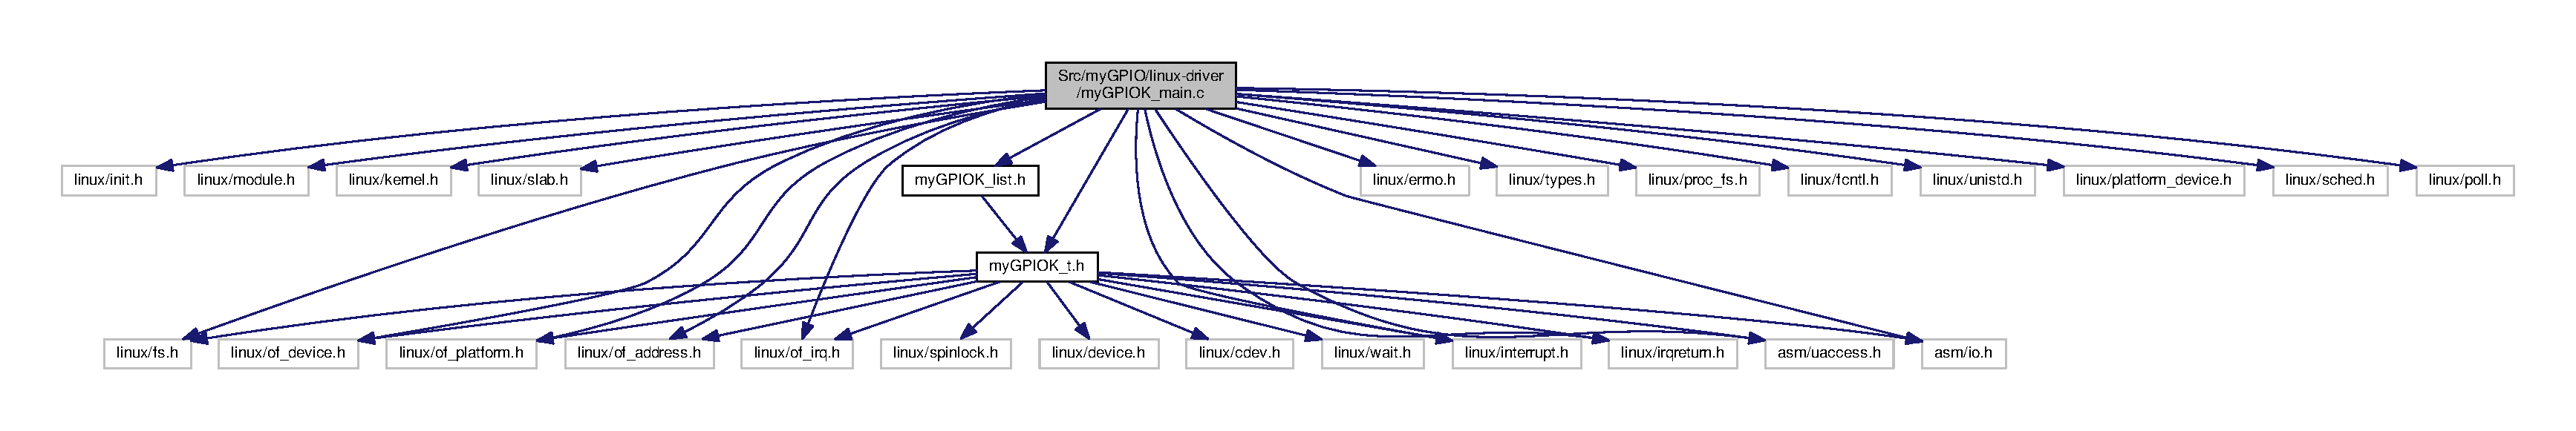
\includegraphics[width=350pt]{my_g_p_i_o_k__main_8c__incl}
\end{center}
\end{figure}
\subsection*{Definizioni}
\begin{DoxyCompactItemize}
\item 
\#define \hyperlink{group___linux-_driver_ga25634d21648ca7fb7a2aca614bafaaeb}{D\+R\+I\+V\+E\+R\+\_\+\+N\+A\+ME}~\char`\"{}my\+G\+P\+I\+OK\char`\"{}
\begin{DoxyCompactList}\small\item\em Nome identificativo del device-\/driver. D\+E\+VE corrispondere al valore del campo \char`\"{}compatible\char`\"{} nel device tree source. \end{DoxyCompactList}\item 
\#define \hyperlink{group___linux-_driver_ga4fa7cb23649a4090e79e2610b7ba0a93}{D\+R\+I\+V\+E\+R\+\_\+\+F\+N\+A\+ME}~\char`\"{}my\+G\+P\+I\+OK\%d\char`\"{}
\begin{DoxyCompactList}\small\item\em Nome del file creato in /dev/ per ciascuno dei device. \end{DoxyCompactList}\item 
\#define \hyperlink{group___linux-_driver_gad32bf20eb64878cb958ca6ac9c96c21d}{M\+A\+X\+\_\+\+N\+U\+M\+\_\+\+O\+F\+\_\+\+D\+E\+V\+I\+C\+ES}~15
\begin{DoxyCompactList}\small\item\em Numero massimo di device gestibili. \end{DoxyCompactList}\item 
\#define \hyperlink{group___linux-_driver_ga78d3a23bb3381a43eaba8bbf8b1cc750}{my\+G\+P\+I\+O\+K\+\_\+\+U\+S\+E\+D\+\_\+\+I\+NT}~0x\+F\+F\+F\+F\+F\+F\+F\+FU
\begin{DoxyCompactList}\small\item\em Maschea di abilitazione degli interrupt per i singoli pin. \end{DoxyCompactList}\end{DoxyCompactItemize}
\subsection*{Funzioni}
\begin{DoxyCompactItemize}
\item 
\hyperlink{group___linux-_driver_gad94b36675e7eb067ea3ce6ff9e244a44}{M\+O\+D\+U\+L\+E\+\_\+\+L\+I\+C\+E\+N\+SE} (\char`\"{}G\+PL\char`\"{})
\item 
\hyperlink{group___linux-_driver_gaa528ef168ff30340d38c46a12fce906b}{M\+O\+D\+U\+L\+E\+\_\+\+A\+U\+T\+H\+OR} (\char`\"{}Salvatore Barone $<$salvator.\+barone@gmail.\+com$>$\char`\"{})
\item 
\hyperlink{group___linux-_driver_ga1a0de0abbfec8f65abc50ccd3a549a4d}{M\+O\+D\+U\+L\+E\+\_\+\+D\+E\+S\+C\+R\+I\+P\+T\+I\+ON} (\char`\"{}my\+G\+P\+IO device-\/driver in kernel mode\char`\"{})
\item 
\hyperlink{group___linux-_driver_ga4d0a47b4ff404d7ced2610438ec9802e}{M\+O\+D\+U\+L\+E\+\_\+\+V\+E\+R\+S\+I\+ON} (\char`\"{}3.\+2\char`\"{})
\item 
\hyperlink{group___linux-_driver_ga1681c4acdb2692baf523dbf58f940399}{M\+O\+D\+U\+L\+E\+\_\+\+A\+L\+I\+AS} (\hyperlink{group___linux-_driver_ga25634d21648ca7fb7a2aca614bafaaeb}{D\+R\+I\+V\+E\+R\+\_\+\+N\+A\+ME})
\item 
static int \hyperlink{group___linux-_driver_gae40973a06d72f7c41a9af07513a62307}{my\+G\+P\+I\+O\+K\+\_\+probe} (struct platform\+\_\+device $\ast$op)
\begin{DoxyCompactList}\small\item\em Viene chiamata quando il modulo viene inserito. \end{DoxyCompactList}\item 
static int \hyperlink{group___linux-_driver_ga59fddfaa36dea357f4bbdfceb0f47f8c}{my\+G\+P\+I\+O\+K\+\_\+remove} (struct platform\+\_\+device $\ast$op)
\item 
static int \hyperlink{group___linux-_driver_gad013759c18fbf6ea96005b9b3bfa5b4e}{my\+G\+P\+I\+O\+K\+\_\+open} (struct inode $\ast$inode, struct file $\ast$file\+\_\+ptr)
\begin{DoxyCompactList}\small\item\em Invocata all\textquotesingle{}apertura del file corrispondente al device. \end{DoxyCompactList}\item 
static int \hyperlink{group___linux-_driver_ga17ce7f574723246c790b70b06e3e7103}{my\+G\+P\+I\+O\+K\+\_\+release} (struct inode $\ast$inode, struct file $\ast$file\+\_\+ptr)
\begin{DoxyCompactList}\small\item\em Invocata alla chiusura del file corrispondente al device. \end{DoxyCompactList}\item 
static loff\+\_\+t \hyperlink{group___linux-_driver_ga66e7f726b72320a272b633ecbaecefff}{my\+G\+P\+I\+O\+K\+\_\+llseek} (struct file $\ast$file\+\_\+ptr, loff\+\_\+t off, int whence)
\begin{DoxyCompactList}\small\item\em Implementa le system-\/call lseek() e llseek(). \end{DoxyCompactList}\item 
static unsigned int \hyperlink{group___linux-_driver_gaba935e8a8215c2ebce9a7147fd4f5147}{my\+G\+P\+I\+O\+K\+\_\+poll} (struct file $\ast$file\+\_\+ptr, struct poll\+\_\+table\+\_\+struct $\ast$wait)
\begin{DoxyCompactList}\small\item\em Verifica che le operazioni di lettura/scrittura risultino non-\/bloccanti. \end{DoxyCompactList}\item 
static ssize\+\_\+t \hyperlink{group___linux-_driver_ga90ac339df9c02ae5f11a2a7727adc923}{my\+G\+P\+I\+O\+K\+\_\+read} (struct file $\ast$file\+\_\+ptr, char $\ast$buf, size\+\_\+t count, loff\+\_\+t $\ast$off)
\begin{DoxyCompactList}\small\item\em Legge dati dal device. \end{DoxyCompactList}\item 
static ssize\+\_\+t \hyperlink{group___linux-_driver_ga1eea0f6c86e8966ba9b701da57502aad}{my\+G\+P\+I\+O\+K\+\_\+write} (struct file $\ast$file\+\_\+ptr, const char $\ast$buf, size\+\_\+t size, loff\+\_\+t $\ast$off)
\begin{DoxyCompactList}\small\item\em Invia dati al device. \end{DoxyCompactList}\item 
static irqreturn\+\_\+t \hyperlink{group___linux-_driver_ga2fc230a12a97aa63e43b2dc4aec73511}{my\+G\+P\+I\+O\+K\+\_\+irq\+\_\+handler} (int irq, struct pt\+\_\+regs $\ast$regs)
\begin{DoxyCompactList}\small\item\em Interrupt-\/handler. \end{DoxyCompactList}\item 
\hyperlink{group___linux-_driver_gaf33e020610cd80a1cfa2ed79b512b841}{M\+O\+D\+U\+L\+E\+\_\+\+D\+E\+V\+I\+C\+E\+\_\+\+T\+A\+B\+LE} (of, \hyperlink{group___linux-_driver_gab59f49dc0fe8d885c73752b8a8163d0e}{my\+G\+P\+I\+O\+K\+\_\+match})
\begin{DoxyCompactList}\small\item\em Inserisce una nuova entry nella tabella delle corrispondenze device -\/ driver. \end{DoxyCompactList}\item 
\hyperlink{group___linux-_driver_ga61e890be90fe5582db8048893ca0ebbf}{module\+\_\+platform\+\_\+driver} (\hyperlink{group___linux-_driver_ga8dba1541b58fa63f8208232ffce4fc47}{my\+G\+P\+I\+O\+K\+\_\+driver})
\begin{DoxyCompactList}\small\item\em la macro \hyperlink{group___linux-_driver_ga61e890be90fe5582db8048893ca0ebbf}{module\+\_\+platform\+\_\+driver()} prende in input la struttura platform\+\_\+driver ed implementa le funzioni module\+\_\+init() e module\+\_\+close() standard, chiamate quando il modulo viene caricato o rimosso dal kernel. \end{DoxyCompactList}\end{DoxyCompactItemize}
\subsection*{Variabili}
\begin{DoxyCompactItemize}
\item 
static \hyperlink{structmy_g_p_i_o_k__list__t}{my\+G\+P\+I\+O\+K\+\_\+list\+\_\+t} $\ast$ \hyperlink{group___linux-_driver_ga1deed297d5c8afeb9703965d37d3be5b}{device\+\_\+list} = N\+U\+LL
\begin{DoxyCompactList}\small\item\em Array di puntatori a struttura \hyperlink{structmy_g_p_i_o_k__t}{my\+G\+P\+I\+O\+K\+\_\+t}, contenente tutti i dati necessari al device driver. \end{DoxyCompactList}\item 
static struct class $\ast$ \hyperlink{group___linux-_driver_gaaf8d1bce7d6389684a037e94381c275c}{my\+G\+P\+I\+O\+K\+\_\+class} = N\+U\+LL
\begin{DoxyCompactList}\small\item\em Classe del device Ai device-\/drivers viene associata una classe ed un device-\/name. Per creare ed associare una classe ad un device driver si può usare la seguente. \end{DoxyCompactList}\item 
static struct of\+\_\+device\+\_\+id \hyperlink{group___linux-_driver_gab59f49dc0fe8d885c73752b8a8163d0e}{my\+G\+P\+I\+O\+K\+\_\+match} \mbox{[}$\,$\mbox{]}
\begin{DoxyCompactList}\small\item\em Identifica il device all\textquotesingle{}interno del device tree. \end{DoxyCompactList}\item 
static struct platform\+\_\+driver \hyperlink{group___linux-_driver_ga8dba1541b58fa63f8208232ffce4fc47}{my\+G\+P\+I\+O\+K\+\_\+driver}
\begin{DoxyCompactList}\small\item\em Definisce quali funzioni probe() e remove() chiamare quando viene caricato un driver. \end{DoxyCompactList}\item 
static struct file\+\_\+operations \hyperlink{group___linux-_driver_gad1963bc01fffdbb315a408a9210cbafc}{my\+G\+P\+I\+O\+K\+\_\+fops}
\begin{DoxyCompactList}\small\item\em mantiene puntatori a funzioni che definiscono il gli operatori che agiscono su un file/device. \end{DoxyCompactList}\end{DoxyCompactItemize}

\hypertarget{my_g_p_i_o_k__t_8c}{}\section{Riferimenti per il file Src/my\+G\+P\+I\+O/linux-\/driver/my\+G\+P\+I\+O\+K\+\_\+t.c}
\label{my_g_p_i_o_k__t_8c}\index{Src/my\+G\+P\+I\+O/linux-\/driver/my\+G\+P\+I\+O\+K\+\_\+t.\+c@{Src/my\+G\+P\+I\+O/linux-\/driver/my\+G\+P\+I\+O\+K\+\_\+t.\+c}}
{\ttfamily \#include \char`\"{}my\+G\+P\+I\+O\+K\+\_\+t.\+h\char`\"{}}\newline
{\ttfamily \#include $<$linux/slab.\+h$>$}\newline
{\ttfamily \#include $<$linux/sched.\+h$>$}\newline
{\ttfamily \#include $<$linux/poll.\+h$>$}\newline
Grafo delle dipendenze di inclusione per my\+G\+P\+I\+O\+K\+\_\+t.\+c\+:\nopagebreak
\begin{figure}[H]
\begin{center}
\leavevmode
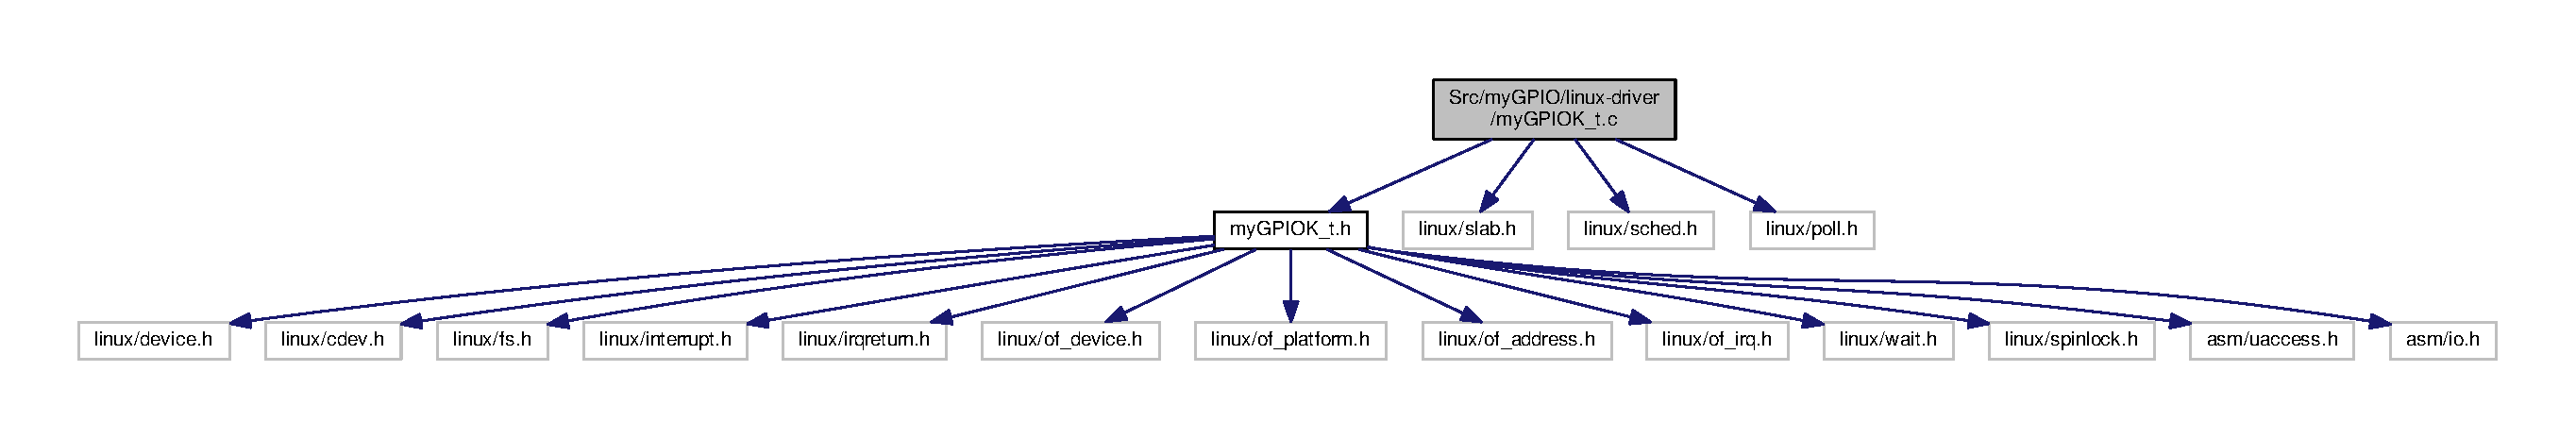
\includegraphics[width=350pt]{my_g_p_i_o_k__t_8c__incl}
\end{center}
\end{figure}
\subsection*{Funzioni}
\begin{DoxyCompactItemize}
\item 
int \hyperlink{group___linux-_driver_ga64afb2eff1f990814d792349842c522d}{my\+G\+P\+I\+O\+K\+\_\+\+Init} (\hyperlink{structmy_g_p_i_o_k__t}{my\+G\+P\+I\+O\+K\+\_\+t} $\ast$my\+G\+P\+I\+O\+K\+\_\+device, struct module $\ast$owner, struct platform\+\_\+device $\ast$op, struct class $\ast$class, const char $\ast$driver\+\_\+name, const char $\ast$device\+\_\+name, uint32\+\_\+t serial, struct file\+\_\+operations $\ast$f\+\_\+ops, irq\+\_\+handler\+\_\+t irq\+\_\+handler, uint32\+\_\+t irq\+\_\+mask)
\begin{DoxyCompactList}\small\item\em Inizializza una struttura \hyperlink{structmy_g_p_i_o_k__t}{my\+G\+P\+I\+O\+K\+\_\+t} e configura il device corrispondente. \end{DoxyCompactList}\item 
void \hyperlink{group___linux-_driver_ga24255b79dd8549aa655cf28c1f9a65d5}{my\+G\+P\+I\+O\+K\+\_\+\+Destroy} (\hyperlink{structmy_g_p_i_o_k__t}{my\+G\+P\+I\+O\+K\+\_\+t} $\ast$device)
\begin{DoxyCompactList}\small\item\em Deinizializza un device, rimuovendo le strutture kernel allocate per il suo funzionamento. \end{DoxyCompactList}\item 
void \hyperlink{group___linux-_driver_gad82c1051e6acb335b1b26ab0c459453b}{my\+G\+P\+I\+O\+K\+\_\+\+Set\+Can\+Read} (\hyperlink{structmy_g_p_i_o_k__t}{my\+G\+P\+I\+O\+K\+\_\+t} $\ast$device)
\begin{DoxyCompactList}\small\item\em Set del flag \char`\"{}interrupt occurred\char`\"{} (can\+Read) \end{DoxyCompactList}\item 
void \hyperlink{group___linux-_driver_ga6dc0ec06b388522ffc524e5fd14d8b72}{my\+G\+P\+I\+O\+K\+\_\+\+Reset\+Can\+Read} (\hyperlink{structmy_g_p_i_o_k__t}{my\+G\+P\+I\+O\+K\+\_\+t} $\ast$device)
\begin{DoxyCompactList}\small\item\em Reset del flag \char`\"{}interrupt occurred\char`\"{} (can\+Read) \end{DoxyCompactList}\item 
void \hyperlink{group___linux-_driver_gaf1b6f35c097c46361d675a42f122828e}{my\+G\+P\+I\+O\+K\+\_\+\+Test\+Can\+Read\+And\+Sleep} (\hyperlink{structmy_g_p_i_o_k__t}{my\+G\+P\+I\+O\+K\+\_\+t} $\ast$device)
\begin{DoxyCompactList}\small\item\em Testa la condizione \char`\"{}interrupt occurred\char`\"{}, mettendo in attesa il processo, se necessario. \end{DoxyCompactList}\item 
unsigned \hyperlink{group___linux-_driver_gae428f50a6da69e3cf89348b8ba9401b1}{my\+G\+P\+I\+O\+K\+\_\+\+Get\+Poll\+Mask} (\hyperlink{structmy_g_p_i_o_k__t}{my\+G\+P\+I\+O\+K\+\_\+t} $\ast$device, struct file $\ast$file\+\_\+ptr, struct poll\+\_\+table\+\_\+struct $\ast$wait)
\begin{DoxyCompactList}\small\item\em Verifica che le operazioni di lettura/scrittura risultino non-\/bloccanti. \end{DoxyCompactList}\item 
void \hyperlink{group___linux-_driver_ga5a7df448de9de94620ce1baf7ec388c9}{my\+G\+P\+I\+O\+K\+\_\+\+Increment\+Total} (\hyperlink{structmy_g_p_i_o_k__t}{my\+G\+P\+I\+O\+K\+\_\+t} $\ast$device)
\begin{DoxyCompactList}\small\item\em Incrementa il contatore degli interrupt per un particolare device. \end{DoxyCompactList}\item 
void \hyperlink{group___linux-_driver_gae182aa943af08c102a05795ae8526192}{my\+G\+P\+I\+O\+K\+\_\+\+Wake\+Up} (\hyperlink{structmy_g_p_i_o_k__t}{my\+G\+P\+I\+O\+K\+\_\+t} $\ast$device)
\begin{DoxyCompactList}\small\item\em Risveglia i process in attesa sulle code di read e poll. \end{DoxyCompactList}\item 
void $\ast$ \hyperlink{group___linux-_driver_ga565ffd4946b330b29e1166dfc9851b11}{my\+G\+P\+I\+O\+K\+\_\+\+Get\+Device\+Address} (\hyperlink{structmy_g_p_i_o_k__t}{my\+G\+P\+I\+O\+K\+\_\+t} $\ast$device)
\begin{DoxyCompactList}\small\item\em Restituisce l\textquotesingle{}indirizzo virtuale di memoria cui è mappato un device. \end{DoxyCompactList}\item 
void \hyperlink{group___linux-_driver_gaf8da20aabceb02b9ea8132228c973368}{my\+G\+P\+I\+O\+K\+\_\+\+Global\+Interrupt\+Enable} (\hyperlink{structmy_g_p_i_o_k__t}{my\+G\+P\+I\+O\+K\+\_\+t} $\ast$device)
\begin{DoxyCompactList}\small\item\em Abilita gli interrupt globali;. \end{DoxyCompactList}\item 
void \hyperlink{group___linux-_driver_gad9275880dc4941d3d0ae93c45bf4cf79}{my\+G\+P\+I\+O\+K\+\_\+\+Global\+Interrupt\+Disable} (\hyperlink{structmy_g_p_i_o_k__t}{my\+G\+P\+I\+O\+K\+\_\+t} $\ast$device)
\begin{DoxyCompactList}\small\item\em Disabilita gli interrupt globali;. \end{DoxyCompactList}\item 
void \hyperlink{group___linux-_driver_gac63adbb81dcfa905341a9ea0bc6283b6}{my\+G\+P\+I\+O\+K\+\_\+\+Pin\+Interrupt\+Enable} (\hyperlink{structmy_g_p_i_o_k__t}{my\+G\+P\+I\+O\+K\+\_\+t} $\ast$device, unsigned mask)
\begin{DoxyCompactList}\small\item\em Abilita gli interrupt per i singoli pin del device. \end{DoxyCompactList}\item 
void \hyperlink{group___linux-_driver_gad600864a578b08a526f8955d3e9f6ca0}{my\+G\+P\+I\+O\+K\+\_\+\+Pin\+Interrupt\+Disable} (\hyperlink{structmy_g_p_i_o_k__t}{my\+G\+P\+I\+O\+K\+\_\+t} $\ast$device, unsigned mask)
\begin{DoxyCompactList}\small\item\em Disabilita gli interrupt per i singoli pin del device. \end{DoxyCompactList}\item 
unsigned \hyperlink{group___linux-_driver_ga3c78c03314722cfa7f32503ede4c29c4}{my\+G\+P\+I\+O\+K\+\_\+\+Pending\+Pin\+Interrupt} (\hyperlink{structmy_g_p_i_o_k__t}{my\+G\+P\+I\+O\+K\+\_\+t} $\ast$device)
\begin{DoxyCompactList}\small\item\em Consente di ottenere una maschera che indichi quali interrupt non siano stati ancora serviti;. \end{DoxyCompactList}\item 
void \hyperlink{group___linux-_driver_ga3c0591dacf65607a7e31a0bf9c9011ae}{my\+G\+P\+I\+O\+K\+\_\+\+Pin\+Interrupt\+Ack} (\hyperlink{structmy_g_p_i_o_k__t}{my\+G\+P\+I\+O\+K\+\_\+t} $\ast$device, unsigned mask)
\begin{DoxyCompactList}\small\item\em Invia al device notifica di servizio di un interrupt;. \end{DoxyCompactList}\end{DoxyCompactItemize}


\subsection{Descrizione dettagliata}
\begin{DoxyAuthor}{Autore}
Salvatore Barone \href{mailto:salvator.barone@gmail.com}{\tt salvator.\+barone@gmail.\+com} 
\end{DoxyAuthor}
\begin{DoxyDate}{Data}
24 06 2017
\end{DoxyDate}
\begin{DoxyCopyright}{Copyright}
Copyright 2017 Salvatore Barone \href{mailto:salvator.barone@gmail.com}{\tt salvator.\+barone@gmail.\+com}
\end{DoxyCopyright}
This file is part of Zynq7000\+Driver\+Pack

Zynq7000\+Driver\+Pack is free software; you can redistribute it and/or modify it under the terms of the G\+NU General Public License as published by the Free Software Foundation; either version 3 of the License, or any later version.

Zynq7000\+Driver\+Pack is distributed in the hope that it will be useful, but W\+I\+T\+H\+O\+UT A\+NY W\+A\+R\+R\+A\+N\+TY; without even the implied warranty of M\+E\+R\+C\+H\+A\+N\+T\+A\+B\+I\+L\+I\+TY or F\+I\+T\+N\+E\+SS F\+OR A P\+A\+R\+T\+I\+C\+U\+L\+AR P\+U\+R\+P\+O\+SE. See the G\+NU General Public License for more details.

You should have received a copy of the G\+NU General Public License along with this program; if not, write to the Free Software Foundation, Inc., 51 Franklin Street, Fifth Floor, Boston, MA 02110-\/1301, U\+SA. 
\hypertarget{my_g_p_i_o_k__t_8h}{}\section{Riferimenti per il file Src/my\+G\+P\+I\+O/linux-\/driver/my\+G\+P\+I\+O\+K\+\_\+t.h}
\label{my_g_p_i_o_k__t_8h}\index{Src/my\+G\+P\+I\+O/linux-\/driver/my\+G\+P\+I\+O\+K\+\_\+t.\+h@{Src/my\+G\+P\+I\+O/linux-\/driver/my\+G\+P\+I\+O\+K\+\_\+t.\+h}}
{\ttfamily \#include $<$linux/device.\+h$>$}\newline
{\ttfamily \#include $<$linux/cdev.\+h$>$}\newline
{\ttfamily \#include $<$linux/fs.\+h$>$}\newline
{\ttfamily \#include $<$linux/interrupt.\+h$>$}\newline
{\ttfamily \#include $<$linux/irqreturn.\+h$>$}\newline
{\ttfamily \#include $<$linux/of\+\_\+device.\+h$>$}\newline
{\ttfamily \#include $<$linux/of\+\_\+platform.\+h$>$}\newline
{\ttfamily \#include $<$linux/of\+\_\+address.\+h$>$}\newline
{\ttfamily \#include $<$linux/of\+\_\+irq.\+h$>$}\newline
{\ttfamily \#include $<$linux/wait.\+h$>$}\newline
{\ttfamily \#include $<$linux/spinlock.\+h$>$}\newline
{\ttfamily \#include $<$asm/uaccess.\+h$>$}\newline
{\ttfamily \#include $<$asm/io.\+h$>$}\newline
Grafo delle dipendenze di inclusione per my\+G\+P\+I\+O\+K\+\_\+t.\+h\+:\nopagebreak
\begin{figure}[H]
\begin{center}
\leavevmode
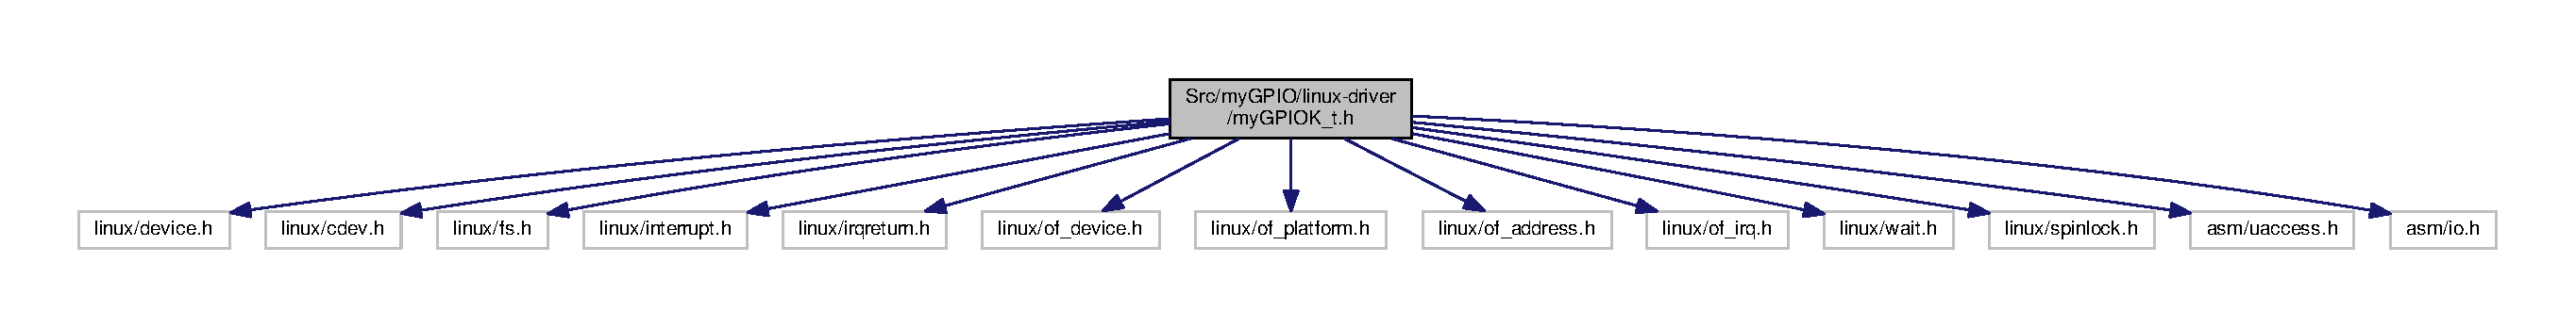
\includegraphics[width=350pt]{my_g_p_i_o_k__t_8h__incl}
\end{center}
\end{figure}
Questo grafo mostra quali altri file includono direttamente o indirettamente questo file\+:\nopagebreak
\begin{figure}[H]
\begin{center}
\leavevmode
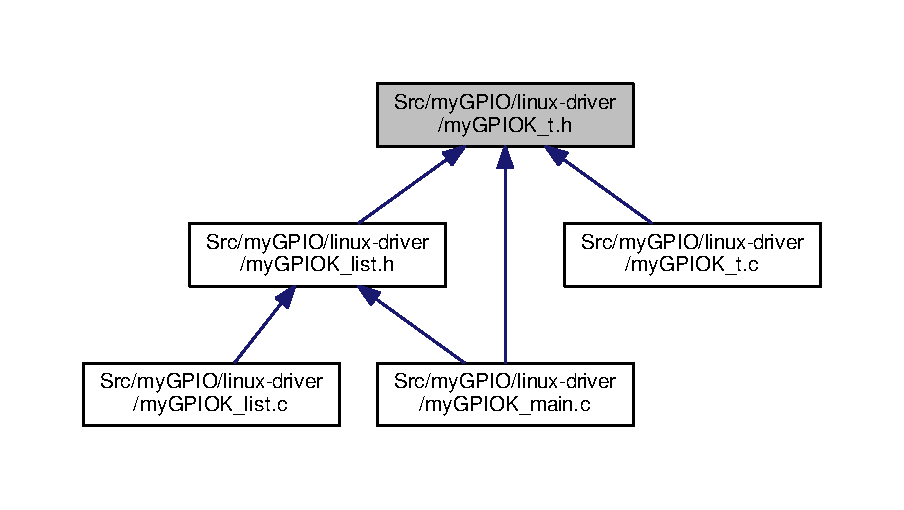
\includegraphics[width=350pt]{my_g_p_i_o_k__t_8h__dep__incl}
\end{center}
\end{figure}
\subsection*{Strutture dati}
\begin{DoxyCompactItemize}
\item 
struct \hyperlink{structmy_g_p_i_o_k__t}{my\+G\+P\+I\+O\+K\+\_\+t}
\begin{DoxyCompactList}\small\item\em Stuttura per l\textquotesingle{}astrazione di un device my\+G\+P\+IO in kernel-\/mode. \end{DoxyCompactList}\end{DoxyCompactItemize}
\subsection*{Definizioni}
\begin{DoxyCompactItemize}
\item 
\#define \hyperlink{group__my_g_p_i_o_k__t_ga0da2526ca3cd1a94ebcecf96778ea2e5}{my\+G\+P\+I\+O\+K\+\_\+\+G\+I\+E\+S\+\_\+\+O\+F\+F\+S\+ET}~0x0\+CU
\begin{DoxyCompactList}\small\item\em Offset, rispetto all\textquotesingle{}indirizzo base, del registro \char`\"{}\+G\+I\+E\+S\char`\"{}. \end{DoxyCompactList}\item 
\#define \hyperlink{group__my_g_p_i_o_k__t_ga2ed7646e6f910f5803477e51b7fe26e3}{my\+G\+P\+I\+O\+K\+\_\+\+P\+I\+E\+\_\+\+O\+F\+F\+S\+ET}~0x10U
\begin{DoxyCompactList}\small\item\em Offset, rispetto all\textquotesingle{}indirizzo base, del registro \char`\"{}\+P\+I\+E\char`\"{}. \end{DoxyCompactList}\item 
\#define \hyperlink{group__my_g_p_i_o_k__t_ga37ee502d1ba364dfde9261c4f7a537a6}{my\+G\+P\+I\+O\+K\+\_\+\+I\+R\+Q\+\_\+\+O\+F\+F\+S\+ET}~0x14U
\begin{DoxyCompactList}\small\item\em Offset, rispetto all\textquotesingle{}indirizzo base, del registro \char`\"{}\+I\+R\+Q\char`\"{}. \end{DoxyCompactList}\item 
\#define \hyperlink{group__my_g_p_i_o_k__t_gac72408c288009c213c0231973b3fe761}{my\+G\+P\+I\+O\+K\+\_\+\+I\+A\+C\+K\+\_\+\+O\+F\+F\+S\+ET}~0x18U
\begin{DoxyCompactList}\small\item\em Offset, rispetto all\textquotesingle{}indirizzo base, del registro \char`\"{}\+I\+A\+C\+K\char`\"{}. \end{DoxyCompactList}\end{DoxyCompactItemize}
\subsection*{Funzioni}
\begin{DoxyCompactItemize}
\item 
int \hyperlink{group__my_g_p_i_o_k__t_ga64afb2eff1f990814d792349842c522d}{my\+G\+P\+I\+O\+K\+\_\+\+Init} (\hyperlink{structmy_g_p_i_o_k__t}{my\+G\+P\+I\+O\+K\+\_\+t} $\ast$my\+G\+P\+I\+O\+K\+\_\+device, struct module $\ast$owner, struct platform\+\_\+device $\ast$op, struct class $\ast$class, const char $\ast$driver\+\_\+name, const char $\ast$device\+\_\+name, uint32\+\_\+t serial, struct file\+\_\+operations $\ast$f\+\_\+ops, irq\+\_\+handler\+\_\+t irq\+\_\+handler, uint32\+\_\+t irq\+\_\+mask)
\begin{DoxyCompactList}\small\item\em Inizializza una struttura \hyperlink{structmy_g_p_i_o_k__t}{my\+G\+P\+I\+O\+K\+\_\+t} e configura il device corrispondente. \end{DoxyCompactList}\item 
void \hyperlink{group__my_g_p_i_o_k__t_ga24255b79dd8549aa655cf28c1f9a65d5}{my\+G\+P\+I\+O\+K\+\_\+\+Destroy} (\hyperlink{structmy_g_p_i_o_k__t}{my\+G\+P\+I\+O\+K\+\_\+t} $\ast$device)
\begin{DoxyCompactList}\small\item\em Deinizializza un device, rimuovendo le strutture kernel allocate per il suo funzionamento. \end{DoxyCompactList}\item 
void \hyperlink{group__my_g_p_i_o_k__t_gad82c1051e6acb335b1b26ab0c459453b}{my\+G\+P\+I\+O\+K\+\_\+\+Set\+Can\+Read} (\hyperlink{structmy_g_p_i_o_k__t}{my\+G\+P\+I\+O\+K\+\_\+t} $\ast$device)
\begin{DoxyCompactList}\small\item\em Set del flag \char`\"{}interrupt occurred\char`\"{} (can\+Read) \end{DoxyCompactList}\item 
void \hyperlink{group__my_g_p_i_o_k__t_ga6dc0ec06b388522ffc524e5fd14d8b72}{my\+G\+P\+I\+O\+K\+\_\+\+Reset\+Can\+Read} (\hyperlink{structmy_g_p_i_o_k__t}{my\+G\+P\+I\+O\+K\+\_\+t} $\ast$device)
\begin{DoxyCompactList}\small\item\em Reset del flag \char`\"{}interrupt occurred\char`\"{} (can\+Read) \end{DoxyCompactList}\item 
void \hyperlink{group__my_g_p_i_o_k__t_gaf1b6f35c097c46361d675a42f122828e}{my\+G\+P\+I\+O\+K\+\_\+\+Test\+Can\+Read\+And\+Sleep} (\hyperlink{structmy_g_p_i_o_k__t}{my\+G\+P\+I\+O\+K\+\_\+t} $\ast$device)
\begin{DoxyCompactList}\small\item\em Testa la condizione \char`\"{}interrupt occurred\char`\"{}, mettendo in attesa il processo, se necessario. \end{DoxyCompactList}\item 
unsigned \hyperlink{group__my_g_p_i_o_k__t_gae428f50a6da69e3cf89348b8ba9401b1}{my\+G\+P\+I\+O\+K\+\_\+\+Get\+Poll\+Mask} (\hyperlink{structmy_g_p_i_o_k__t}{my\+G\+P\+I\+O\+K\+\_\+t} $\ast$device, struct file $\ast$file\+\_\+ptr, struct poll\+\_\+table\+\_\+struct $\ast$wait)
\begin{DoxyCompactList}\small\item\em Verifica che le operazioni di lettura/scrittura risultino non-\/bloccanti. \end{DoxyCompactList}\item 
void \hyperlink{group__my_g_p_i_o_k__t_ga5a7df448de9de94620ce1baf7ec388c9}{my\+G\+P\+I\+O\+K\+\_\+\+Increment\+Total} (\hyperlink{structmy_g_p_i_o_k__t}{my\+G\+P\+I\+O\+K\+\_\+t} $\ast$device)
\begin{DoxyCompactList}\small\item\em Incrementa il contatore degli interrupt per un particolare device. \end{DoxyCompactList}\item 
void \hyperlink{group__my_g_p_i_o_k__t_gae182aa943af08c102a05795ae8526192}{my\+G\+P\+I\+O\+K\+\_\+\+Wake\+Up} (\hyperlink{structmy_g_p_i_o_k__t}{my\+G\+P\+I\+O\+K\+\_\+t} $\ast$device)
\begin{DoxyCompactList}\small\item\em Risveglia i process in attesa sulle code di read e poll. \end{DoxyCompactList}\item 
void $\ast$ \hyperlink{group__my_g_p_i_o_k__t_ga565ffd4946b330b29e1166dfc9851b11}{my\+G\+P\+I\+O\+K\+\_\+\+Get\+Device\+Address} (\hyperlink{structmy_g_p_i_o_k__t}{my\+G\+P\+I\+O\+K\+\_\+t} $\ast$device)
\begin{DoxyCompactList}\small\item\em Restituisce l\textquotesingle{}indirizzo virtuale di memoria cui è mappato un device. \end{DoxyCompactList}\item 
void \hyperlink{group__my_g_p_i_o_k__t_ga00a24f28b49c71aaa91f66be71a3895b}{my\+G\+P\+I\+O\+K\+\_\+\+Global\+Interrupt\+Enable} (\hyperlink{structmy_g_p_i_o_k__t}{my\+G\+P\+I\+O\+K\+\_\+t} $\ast$my\+G\+P\+I\+O\+K\+\_\+device)
\begin{DoxyCompactList}\small\item\em Abilita gli interrupt globali;. \end{DoxyCompactList}\item 
void \hyperlink{group__my_g_p_i_o_k__t_gace0d81f5ec65978f22118a3f1fc8b222}{my\+G\+P\+I\+O\+K\+\_\+\+Global\+Interrupt\+Disable} (\hyperlink{structmy_g_p_i_o_k__t}{my\+G\+P\+I\+O\+K\+\_\+t} $\ast$my\+G\+P\+I\+O\+K\+\_\+device)
\begin{DoxyCompactList}\small\item\em Disabilita gli interrupt globali;. \end{DoxyCompactList}\item 
void \hyperlink{group__my_g_p_i_o_k__t_ga179c20f5f62e8ce1593cbedff2f00533}{my\+G\+P\+I\+O\+K\+\_\+\+Pin\+Interrupt\+Enable} (\hyperlink{structmy_g_p_i_o_k__t}{my\+G\+P\+I\+O\+K\+\_\+t} $\ast$my\+G\+P\+I\+O\+K\+\_\+device, unsigned mask)
\begin{DoxyCompactList}\small\item\em Abilita gli interrupt per i singoli pin del device. \end{DoxyCompactList}\item 
void \hyperlink{group__my_g_p_i_o_k__t_gabfd91641f98a4725aec779c8834ca92d}{my\+G\+P\+I\+O\+K\+\_\+\+Pin\+Interrupt\+Disable} (\hyperlink{structmy_g_p_i_o_k__t}{my\+G\+P\+I\+O\+K\+\_\+t} $\ast$my\+G\+P\+I\+O\+K\+\_\+device, unsigned mask)
\begin{DoxyCompactList}\small\item\em Disabilita gli interrupt per i singoli pin del device. \end{DoxyCompactList}\item 
unsigned \hyperlink{group__my_g_p_i_o_k__t_ga1b3ad44b9198f537493180d748de0b6c}{my\+G\+P\+I\+O\+K\+\_\+\+Pending\+Pin\+Interrupt} (\hyperlink{structmy_g_p_i_o_k__t}{my\+G\+P\+I\+O\+K\+\_\+t} $\ast$my\+G\+P\+I\+O\+K\+\_\+device)
\begin{DoxyCompactList}\small\item\em Consente di ottenere una maschera che indichi quali interrupt non siano stati ancora serviti;. \end{DoxyCompactList}\item 
void \hyperlink{group__my_g_p_i_o_k__t_ga8eaf8f1b21aa6f772c395faf457144f9}{my\+G\+P\+I\+O\+K\+\_\+\+Pin\+Interrupt\+Ack} (\hyperlink{structmy_g_p_i_o_k__t}{my\+G\+P\+I\+O\+K\+\_\+t} $\ast$my\+G\+P\+I\+O\+K\+\_\+device, unsigned mask)
\begin{DoxyCompactList}\small\item\em Invia al device notifica di servizio di un interrupt;. \end{DoxyCompactList}\end{DoxyCompactItemize}


\subsection{Descrizione dettagliata}
\begin{DoxyAuthor}{Autore}
Salvatore Barone \href{mailto:salvator.barone@gmail.com}{\tt salvator.\+barone@gmail.\+com} 
\end{DoxyAuthor}
\begin{DoxyDate}{Data}
24 06 2017
\end{DoxyDate}
\begin{DoxyCopyright}{Copyright}
Copyright 2017 Salvatore Barone \href{mailto:salvator.barone@gmail.com}{\tt salvator.\+barone@gmail.\+com}
\end{DoxyCopyright}
This file is part of Zynq7000\+Driver\+Pack

Zynq7000\+Driver\+Pack is free software; you can redistribute it and/or modify it under the terms of the G\+NU General Public License as published by the Free Software Foundation; either version 3 of the License, or any later version.

Zynq7000\+Driver\+Pack is distributed in the hope that it will be useful, but W\+I\+T\+H\+O\+UT A\+NY W\+A\+R\+R\+A\+N\+TY; without even the implied warranty of M\+E\+R\+C\+H\+A\+N\+T\+A\+B\+I\+L\+I\+TY or F\+I\+T\+N\+E\+SS F\+OR A P\+A\+R\+T\+I\+C\+U\+L\+AR P\+U\+R\+P\+O\+SE. See the G\+NU General Public License for more details.

You should have received a copy of the G\+NU General Public License along with this program; if not, write to the Free Software Foundation, Inc., 51 Franklin Street, Fifth Floor, Boston, MA 02110-\/1301, U\+SA. 
\chapter{Documentazione degli esempi}
\hypertarget{interrupt_bare_8c-example}{\section{interrupt\+\_\+bare.\+c}
}
Uso del driver my\+G\+P\+I\+O con interruzioni bare-\/metal su Zynq-\/7000 \begin{DoxyAuthor}{Autore}
Salvatore Barone \href{mailto:salvator.barone@gmail.com}{\tt salvator.\+barone@gmail.\+com} 
\end{DoxyAuthor}
\begin{DoxyDate}{Data}
23 06 2017
\end{DoxyDate}
\begin{DoxyCopyright}{Copyright}
Copyright 2017 Salvatore Barone \href{mailto:salvator.barone@gmail.com}{\tt salvator.\+barone@gmail.\+com}
\end{DoxyCopyright}
This file is part of Zynq7000\+Driver\+Pack

Zynq7000\+Driver\+Pack is free software; you can redistribute it and/or modify it under the terms of the G\+N\+U General Public License as published by the Free Software Foundation; either version 3 of the License, or any later version.

Zynq7000\+Driver\+Pack is distributed in the hope that it will be useful, but W\+I\+T\+H\+O\+U\+T A\+N\+Y W\+A\+R\+R\+A\+N\+T\+Y; without even the implied warranty of M\+E\+R\+C\+H\+A\+N\+T\+A\+B\+I\+L\+I\+T\+Y or F\+I\+T\+N\+E\+S\+S F\+O\+R A P\+A\+R\+T\+I\+C\+U\+L\+A\+R P\+U\+R\+P\+O\+S\+E. See the G\+N\+U General Public License for more details.

You should have received a copy of the G\+N\+U General Public License along with this program; if not, write to the Free Software Foundation, Inc., 51 Franklin Street, Fifth Floor, Boston, M\+A 02110-\/1301, U\+S\+A.

\paragraph*{Configurazione hardware}

L'esempio fa riferimento ad una configurazione hardware in cui, oltre alla ip-\/core Zynq7000 processing sysyem, sono presenti tre diversi device my\+G\+P\+I\+O, uno connesso ai led (base address 0x43c00000), uno connesso ai button (base address 0x43c10000) ed uno connesso agli switch (base address 0x43c20000). Lo schema viene riportato di seguito\+: 

\subparagraph*{I\+S\+R per la gestione di interrupt provenienti dal gpio connesso agli switch}


\begin{DoxyCode}
\textcolor{keywordtype}{void} \hyperlink{interrupt__bare_8c_ad05dc46b6c6da383d687c5116864b4ed}{swc\_isr}(\textcolor{keywordtype}{void}* data) \{
    \hyperlink{group__bare-metal_gaacca2871ac57a166e62bf431a2da7548}{myGPIO\_GlobalInterruptDisable}(&swc\_gpio);
    \hyperlink{group__bare-metal_ga402a0d20afc0cb7c25554b8b023f4253}{myGPIO\_mask} enabledInterrut = \hyperlink{group__bare-metal_ga80ef1cf3e9bd8bfd4d849a0f3b8e7b2c}{myGPIO\_EnabledPinInterrupt}(&swc\_gpio
      );
    \hyperlink{group__bare-metal_ga37d3df33ac50387d6f2e1fb5e2b13e49}{myGPIO\_PinInterruptDisable}(&swc\_gpio, enabledInterrut);

    \hyperlink{group__bare-metal_ga402a0d20afc0cb7c25554b8b023f4253}{myGPIO\_mask} pendingInterrupt = \hyperlink{group__bare-metal_ga6115bde39f860d4e76e7d8f421ce222c}{myGPIO\_PendingPinInterrupt}(&
      swc\_gpio);
    \hyperlink{group__bare-metal_gab6ad3dda867515825890c97dbf6f55db}{myGPIO\_PinInterruptAck}(&swc\_gpio, pendingInterrupt);

    \hyperlink{group__bare-metal_ga402a0d20afc0cb7c25554b8b023f4253}{myGPIO\_mask} value = \hyperlink{group__bare-metal_gac35776cd6652f7b932a132f3f6959a11}{myGPIO\_GetRead}(&swc\_gpio);
    \hyperlink{group__bare-metal_ga9d9ce9d2db7d77a588da4a3749f2f24d}{myGPIO\_SetValue}(&led\_gpio, \hyperlink{group__bare-metal_gga402a0d20afc0cb7c25554b8b023f4253a6db6fa7be955ae379f543d96122e23a9}{myGPIO\_pin0} | 
      \hyperlink{group__bare-metal_gga402a0d20afc0cb7c25554b8b023f4253a1de6bdcc01efca2c39f584f5a20293be}{myGPIO\_pin1} | \hyperlink{group__bare-metal_gga402a0d20afc0cb7c25554b8b023f4253a1fb3f52d920ac8ba17b74dd73c27d783}{myGPIO\_pin2} | \hyperlink{group__bare-metal_gga402a0d20afc0cb7c25554b8b023f4253a4514d64390392b626aa4dbfaac8dc1e5}{myGPIO\_pin3}, 
      \hyperlink{group__bare-metal_ggaf634fe4a0e1eab8da5000b72d6ad362ba98cde80dbda025bd1ae7231c76b55674}{myGPIO\_reset});
    \hyperlink{group__bare-metal_ga9d9ce9d2db7d77a588da4a3749f2f24d}{myGPIO\_SetValue}(&led\_gpio, value, \hyperlink{group__bare-metal_ggaf634fe4a0e1eab8da5000b72d6ad362ba10d296f3711d01189cc6c2d87f7c9149}{myGPIO\_set});

    \hyperlink{group__bare-metal_ga116e3a1077a317e9e42ded6dd4df64af}{myGPIO\_PinInterruptEnable}(&swc\_gpio, enabledInterrut);
    \hyperlink{group__bare-metal_gada93ef6a9818e634f0a233ce14582216}{myGPIO\_GlobalInterruptEnable}(&swc\_gpio);
\}
\end{DoxyCode}
 La funzione di cui sopra non fa altro che disabilitare momentaneamente le interruzioni della periferica, leggere lo stato del registro “read”, resettare i led, per poi accendere solo quello corrispondente allo switch arrivo e riabilitare l'interrupt della periferica.

\subparagraph*{I\+S\+R per la gestione di interrupt provenienti dal gpio connesso ai button}


\begin{DoxyCode}
\textcolor{keywordtype}{void} \hyperlink{interrupt__bare_8c_aa4eac585cb67311e3e5fd374d6b09ad4}{btn\_isr}(\textcolor{keywordtype}{void}* data) \{
    \hyperlink{group__bare-metal_gaacca2871ac57a166e62bf431a2da7548}{myGPIO\_GlobalInterruptDisable}(&btn\_gpio);
    \hyperlink{group__bare-metal_ga402a0d20afc0cb7c25554b8b023f4253}{myGPIO\_mask} enabledInterrut = \hyperlink{group__bare-metal_ga80ef1cf3e9bd8bfd4d849a0f3b8e7b2c}{myGPIO\_EnabledPinInterrupt}(&btn\_gpio
      );
    \hyperlink{group__bare-metal_ga37d3df33ac50387d6f2e1fb5e2b13e49}{myGPIO\_PinInterruptDisable}(&btn\_gpio, enabledInterrut);

    \hyperlink{group__bare-metal_ga402a0d20afc0cb7c25554b8b023f4253}{myGPIO\_mask} pendingInterrupt = \hyperlink{group__bare-metal_ga6115bde39f860d4e76e7d8f421ce222c}{myGPIO\_PendingPinInterrupt}(&
      btn\_gpio);
    \hyperlink{group__bare-metal_gab6ad3dda867515825890c97dbf6f55db}{myGPIO\_PinInterruptAck}(&btn\_gpio, pendingInterrupt);

    \hyperlink{group__bare-metal_ga402a0d20afc0cb7c25554b8b023f4253}{myGPIO\_mask} value = \hyperlink{group__bare-metal_gac35776cd6652f7b932a132f3f6959a11}{myGPIO\_GetRead}(&btn\_gpio);
    \hyperlink{group__bare-metal_ga9d9ce9d2db7d77a588da4a3749f2f24d}{myGPIO\_SetValue}(&led\_gpio, \hyperlink{group__bare-metal_gga402a0d20afc0cb7c25554b8b023f4253a6db6fa7be955ae379f543d96122e23a9}{myGPIO\_pin0} | 
      \hyperlink{group__bare-metal_gga402a0d20afc0cb7c25554b8b023f4253a1de6bdcc01efca2c39f584f5a20293be}{myGPIO\_pin1} | \hyperlink{group__bare-metal_gga402a0d20afc0cb7c25554b8b023f4253a1fb3f52d920ac8ba17b74dd73c27d783}{myGPIO\_pin2} | \hyperlink{group__bare-metal_gga402a0d20afc0cb7c25554b8b023f4253a4514d64390392b626aa4dbfaac8dc1e5}{myGPIO\_pin3}, 
      \hyperlink{group__bare-metal_ggaf634fe4a0e1eab8da5000b72d6ad362ba98cde80dbda025bd1ae7231c76b55674}{myGPIO\_reset});
    \hyperlink{group__bare-metal_ga9d9ce9d2db7d77a588da4a3749f2f24d}{myGPIO\_SetValue}(&led\_gpio, value, \hyperlink{group__bare-metal_ggaf634fe4a0e1eab8da5000b72d6ad362ba10d296f3711d01189cc6c2d87f7c9149}{myGPIO\_set});

    \hyperlink{group__bare-metal_ga116e3a1077a317e9e42ded6dd4df64af}{myGPIO\_PinInterruptEnable}(&btn\_gpio, enabledInterrut);
    \hyperlink{group__bare-metal_gada93ef6a9818e634f0a233ce14582216}{myGPIO\_GlobalInterruptEnable}(&btn\_gpio);
\}
\end{DoxyCode}
 La funzione di cui sopra non fa altro che disabilitare momentaneamente le interruzioni della periferica, leggere lo stato del registro “read”, resettare i led, per poi accendere solo quello corrispondente al button premuto e riabilitare l'interrupt della periferica.

\subparagraph*{Configurazione del G\+I\+C e registrazione degli interrupt handler}


\begin{DoxyCode}
\textcolor{keywordtype}{int} \hyperlink{interrupt__bare_8c_ad4c208e7b28dadf641bc3ec5b290d87d}{int\_config}(\textcolor{keywordtype}{void}) \{
    \textcolor{comment}{// inizializza il driver del GIC}
    Xil\_ExceptionInit();

    \textcolor{comment}{// ottiene i parametri di configurazione del GIC, lo configura ed inizializza}
    \textcolor{comment}{// sintassi : XScuGic\_LookupConfig(GIC\_id)}
    \textcolor{comment}{// sintassi : XScuGic\_CfgInitialize(GIC\_ptr, config, cpu\_address)}
    XScuGic\_Config *IntcConfig = XScuGic\_LookupConfig(\hyperlink{interrupt__bare_8c_a22782ed5aaa2e8d89334d159d14753b5}{gic\_id});
    \textcolor{keywordflow}{if} (IntcConfig == NULL)
        \textcolor{keywordflow}{return} -1;
    \textcolor{keywordflow}{if} (XScuGic\_CfgInitialize(&\hyperlink{interrupt__bare_8c_a0ad1175dbe99ac3f36c814258ec4f8c6}{GIC}, IntcConfig, IntcConfig->CpuBaseAddress) != XST\_SUCCESS)
        \textcolor{keywordflow}{return} -1;

    \textcolor{comment}{// registra l'interrupt handler del GIC alla logica di gestione del processing-system}
    \textcolor{comment}{// sintassi : Xil\_ExceptionRegisterHandler(XIL\_EXCEPTION\_ID\_INT, handler, gic\_ptr)}
    Xil\_ExceptionRegisterHandler(XIL\_EXCEPTION\_ID\_INT,(Xil\_ExceptionHandler)XScuGic\_InterruptHandler, &
      \hyperlink{interrupt__bare_8c_a0ad1175dbe99ac3f36c814258ec4f8c6}{GIC});

    \textcolor{comment}{// registrazione degli handler}
    \textcolor{comment}{// le righe seguenti stabiliscono quale sia l'handler da chiamare e quali dati bisogna passargli}
    \textcolor{comment}{// qualora si manifesti una interruzione su una line di irq.}
    \textcolor{comment}{// sintassi : XScuGic\_Connect(GIC, irq\_line, handler, data)}
    \textcolor{keywordflow}{if} (XScuGic\_Connect(&\hyperlink{interrupt__bare_8c_a0ad1175dbe99ac3f36c814258ec4f8c6}{GIC}, \hyperlink{interrupt__bare_8c_ab5602e3672ec6d03f39d2229dbcb9f74}{btn\_irq\_line}, (Xil\_InterruptHandler)btn\_isr, (\textcolor{keywordtype}{void}*)NULL) != 
      XST\_SUCCESS)
        \textcolor{keywordflow}{return} -1;
    \textcolor{keywordflow}{if} (XScuGic\_Connect(&\hyperlink{interrupt__bare_8c_a0ad1175dbe99ac3f36c814258ec4f8c6}{GIC}, \hyperlink{interrupt__bare_8c_a48d05dc71b54a160af13c8e31e9000b1}{swc\_irq\_line}, (Xil\_InterruptHandler)swc\_isr, (\textcolor{keywordtype}{void}*)NULL) != 
      XST\_SUCCESS)
            \textcolor{keywordflow}{return} -1;

    \textcolor{comment}{// abilitazione degli interrupt sulle linee connesse alle periferiche}
    \textcolor{comment}{// sintassi: XScuGic\_Enable(GIC,irq\_line);}
    XScuGic\_Enable(&\hyperlink{interrupt__bare_8c_a0ad1175dbe99ac3f36c814258ec4f8c6}{GIC}, \hyperlink{interrupt__bare_8c_ab5602e3672ec6d03f39d2229dbcb9f74}{btn\_irq\_line});
    XScuGic\_Enable(&\hyperlink{interrupt__bare_8c_a0ad1175dbe99ac3f36c814258ec4f8c6}{GIC}, \hyperlink{interrupt__bare_8c_a48d05dc71b54a160af13c8e31e9000b1}{swc\_irq\_line});

    \textcolor{comment}{// abilitazione degli interrupt delle periferiche}
    \hyperlink{group__bare-metal_gada93ef6a9818e634f0a233ce14582216}{myGPIO\_GlobalInterruptEnable}(&btn\_gpio);
    \hyperlink{group__bare-metal_ga116e3a1077a317e9e42ded6dd4df64af}{myGPIO\_PinInterruptEnable}(&btn\_gpio, \hyperlink{group__bare-metal_gga402a0d20afc0cb7c25554b8b023f4253a6db6fa7be955ae379f543d96122e23a9}{myGPIO\_pin0} | 
      \hyperlink{group__bare-metal_gga402a0d20afc0cb7c25554b8b023f4253a1de6bdcc01efca2c39f584f5a20293be}{myGPIO\_pin1} | \hyperlink{group__bare-metal_gga402a0d20afc0cb7c25554b8b023f4253a1fb3f52d920ac8ba17b74dd73c27d783}{myGPIO\_pin2} | \hyperlink{group__bare-metal_gga402a0d20afc0cb7c25554b8b023f4253a4514d64390392b626aa4dbfaac8dc1e5}{myGPIO\_pin3});
    \hyperlink{group__bare-metal_gada93ef6a9818e634f0a233ce14582216}{myGPIO\_GlobalInterruptEnable}(&swc\_gpio);
    \hyperlink{group__bare-metal_ga116e3a1077a317e9e42ded6dd4df64af}{myGPIO\_PinInterruptEnable}(&swc\_gpio, \hyperlink{group__bare-metal_gga402a0d20afc0cb7c25554b8b023f4253a6db6fa7be955ae379f543d96122e23a9}{myGPIO\_pin0} | 
      \hyperlink{group__bare-metal_gga402a0d20afc0cb7c25554b8b023f4253a1de6bdcc01efca2c39f584f5a20293be}{myGPIO\_pin1} | \hyperlink{group__bare-metal_gga402a0d20afc0cb7c25554b8b023f4253a1fb3f52d920ac8ba17b74dd73c27d783}{myGPIO\_pin2} | \hyperlink{group__bare-metal_gga402a0d20afc0cb7c25554b8b023f4253a4514d64390392b626aa4dbfaac8dc1e5}{myGPIO\_pin3});

    \textcolor{comment}{// abilitazione degli interrupt del processing-system}
    Xil\_ExceptionEnable();
    \textcolor{keywordflow}{return} 0;
\}
\end{DoxyCode}
 La funzione di configurazione delle interrupt e del G\+I\+C fa uso di alcune funzioni di libreria definite nell'header file \char`\"{}xscugic.\+h\char`\"{}, il quale implementa il driver della periferica G\+I\+C, e di alcune macro definite nel file \char`\"{}xparameters.\+h\char`\"{}. Solo per comodità le macro definite in xparameters.\+h sono state ridefinite come segue. 
\begin{DoxyCode}
\textcolor{preprocessor}{#define led\_base\_addr XPAR\_MYGPIO\_0\_S00\_AXI\_BASEADDR}
\textcolor{preprocessor}{#define btn\_base\_addr XPAR\_MYGPIO\_1\_S00\_AXI\_BASEADDR}
\textcolor{preprocessor}{#define swc\_base\_addr XPAR\_MYGPIO\_2\_S00\_AXI\_BASEADDR}
\textcolor{preprocessor}{#define led\_irq\_line XPAR\_FABRIC\_MYGPIO\_0\_INTERRUPT\_INTR}
\textcolor{preprocessor}{#define btn\_irq\_line XPAR\_FABRIC\_MYGPIO\_1\_INTERRUPT\_INTR}
\textcolor{preprocessor}{#define swc\_irq\_line XPAR\_FABRIC\_MYGPIO\_2\_INTERRUPT\_INTR}
\textcolor{preprocessor}{#define gic\_id      XPAR\_SCUGIC\_0\_DEVICE\_ID}
\end{DoxyCode}
 Le funzioni di libreria usate sono riportate di seguito, assieme ad una breve descrizione tratta dalla documentazione interna.
\begin{DoxyItemize}
\item Xil\+\_\+\+Exception\+Init()\+: inizializza gli exception-\/handlers di tutti i processori. Per A\+R\+M Cortex A53, R5 ed A9 gli exception-\/handlers sono sono inizializzati staticamente, per cui questa funzione non fa niente. Viene mantenutaper prevenire errori in fase di compilazione e per garantire backward-\/compatibility.
\item X\+Scu\+Gic\+\_\+\+Lookup\+Config()\+: looksup della configurazione di un device, basandosi sull'identificativo univoco dello stesso, dalla tabella contenente le configurazioni di tutti i device. Prende in ingresso un parametro Device\+Id e restituisce un puntatore a X\+Scu\+Gic, contenente la configurazione, o N\+U\+L\+L se il device non viene trovato.
\item X\+Scu\+Gic\+\_\+\+Cfg\+Initialize()\+: inizializza e configura un interrupt-\/controller instance/driver. La procedura di inizializzazione prevede\+:
\begin{DoxyItemize}
\item l'inizializzazione dei campi di una struttura X\+Scu\+Gic;
\item la configurazione della Initial vector-\/table, con funzioni stub;
\item disabilitazione di tutte le sorgenti di interruzione
\end{DoxyItemize}Parametri\+:
\begin{DoxyItemize}
\item Instance\+Ptr\+: puntatore a struttura X\+Scu\+Gic;
\item Config\+Ptr\+: puntatore alla configurazione del device, restituito dalla funzione X\+Scu\+Gic\+\_\+\+Lookup\+Config();
\item Effective\+Addr\+: indirizzo base del device; Restituisce X\+S\+T\+\_\+\+S\+U\+C\+C\+E\+S\+S se l'inizializzazione viene completata con successo.
\end{DoxyItemize}
\item Xil\+\_\+\+Exception\+Register\+Handler()\+: crea una connessione tra l'identificativo di una sorgente di eccezioni e l'handler associato, in modo che l'handler venga eseguito qualora si manifestasse una eccezione. Prende i seguenti parametri\+:
\begin{DoxyItemize}
\item exception\+\_\+id\+: I\+D della sorgente di eccezioni;
\item Handler\+: puntatore alla funzione di servizio;
\item Data\+: puntatore ai dati da passare all'handler;
\end{DoxyItemize}
\item X\+Scu\+Gic\+\_\+\+Connect()\+: crea una connessione tra l'identificativo di una sorgente di interruzioni e l'handler associato, in modo che l'handler venga eseguito qualora si manifestasse una interruzione. Prende i seguenti parametri\+:
\begin{DoxyItemize}
\item Instance\+Ptr\+: puntatore ad una istanza X\+Scu\+Gic;
\item Int\+\_\+\+Id\+: I\+D della sorgente di interruzioni;
\item Handler\+: puntatore alla funzione di servizio;
\item Call\+Back\+Ref\+: puntatore ai dati da passare alla isr;
\end{DoxyItemize}Restituisce X\+S\+T\+\_\+\+S\+U\+C\+C\+E\+S\+S se l'handler è stato connesso correttamente.
\item X\+Scu\+Gic\+\_\+\+Enable()\+: abilita la sorgente di interruzioni Int\+\_\+\+Id. Se ci sono pending interrupt per tale linea, scateneranno una interruzione dopo la chiamata a questa funzione. Parametri\+:
\begin{DoxyItemize}
\item Instance\+Ptr\+: puntatore ad una istanza X\+Scu\+Gic;
\item Int\+\_\+\+Id\+: I\+D della sorgente di interruzioni;
\end{DoxyItemize}
\item Xil\+\_\+\+Exception\+Enable()\+: abilita le interruzioni.
\end{DoxyItemize}


\begin{DoxyCodeInclude}

\textcolor{preprocessor}{#include "xparameters.h"}
\textcolor{preprocessor}{#include "xscugic.h"}
\textcolor{preprocessor}{#include "\hyperlink{my_g_p_i_o_8h}{myGPIO.h}"}

\hyperlink{structmy_g_p_i_o__t}{myGPIO\_t} \hyperlink{interrupt__bare_8c_ac523aaaf082570c199faf2a98e03c219}{led\_gpio};
\hyperlink{structmy_g_p_i_o__t}{myGPIO\_t} \hyperlink{interrupt__bare_8c_ac77d5df697b8a0d64704dee5f1433832}{btn\_gpio};
\hyperlink{structmy_g_p_i_o__t}{myGPIO\_t} \hyperlink{interrupt__bare_8c_ac2f1233c00752afeb2ecfd305c5fe36a}{swc\_gpio};
XScuGic \hyperlink{interrupt__bare_8c_a0ad1175dbe99ac3f36c814258ec4f8c6}{GIC};

\textcolor{preprocessor}{#define led\_base\_addr XPAR\_MYGPIO\_0\_S00\_AXI\_BASEADDR}
\textcolor{preprocessor}{#define btn\_base\_addr XPAR\_MYGPIO\_1\_S00\_AXI\_BASEADDR}
\textcolor{preprocessor}{#define swc\_base\_addr XPAR\_MYGPIO\_2\_S00\_AXI\_BASEADDR}

\textcolor{preprocessor}{#define led\_irq\_line XPAR\_FABRIC\_MYGPIO\_0\_INTERRUPT\_INTR}
\textcolor{preprocessor}{#define btn\_irq\_line XPAR\_FABRIC\_MYGPIO\_1\_INTERRUPT\_INTR}
\textcolor{preprocessor}{#define swc\_irq\_line XPAR\_FABRIC\_MYGPIO\_2\_INTERRUPT\_INTR}

\textcolor{preprocessor}{#define gic\_id      XPAR\_SCUGIC\_0\_DEVICE\_ID}

\textcolor{comment}{// funzione di inizializzazione dei device gpio}
\textcolor{keywordtype}{void} \hyperlink{interrupt__bare_8c_afdbe206b3c49f019757ab09b3cf52b9c}{gpio\_init}(\textcolor{keywordtype}{void});

\textcolor{comment}{// isr per button e switch}
\textcolor{comment}{// devono necessariamente avere questa firma: restituire void e possedere un solo parametro puntatore}
\textcolor{comment}{// a void. In questo caso non viene utilizzato (tutte le variabili sono globali), ma tale puntatore}
\textcolor{comment}{// può essere usato per scambiare dati di ingresso/uscita alle isr}
\textcolor{keywordtype}{void} \hyperlink{interrupt__bare_8c_aa4eac585cb67311e3e5fd374d6b09ad4}{btn\_isr}(\textcolor{keywordtype}{void}*); \textcolor{comment}{// isr per i button}
\textcolor{keywordtype}{void} \hyperlink{interrupt__bare_8c_ad05dc46b6c6da383d687c5116864b4ed}{swc\_isr}(\textcolor{keywordtype}{void}*); \textcolor{comment}{// isr per gli switch}

\textcolor{comment}{// funzione di configurazione del device gic e delle interruzioni}
\textcolor{keywordtype}{int} \hyperlink{interrupt__bare_8c_ad4c208e7b28dadf641bc3ec5b290d87d}{int\_config}(\textcolor{keywordtype}{void});

\textcolor{keywordtype}{int} \hyperlink{interrupt__bare_8c_ae66f6b31b5ad750f1fe042a706a4e3d4}{main}() \{
    \hyperlink{interrupt__bare_8c_afdbe206b3c49f019757ab09b3cf52b9c}{gpio\_init}();
    \hyperlink{interrupt__bare_8c_ad4c208e7b28dadf641bc3ec5b290d87d}{int\_config}();
    \textcolor{keywordflow}{for} (;;);
    \textcolor{keywordflow}{return} 0;
\}

\textcolor{keywordtype}{void} \hyperlink{interrupt__bare_8c_afdbe206b3c49f019757ab09b3cf52b9c}{gpio\_init}(\textcolor{keywordtype}{void}) \{
    uint8\_t i;

    \hyperlink{group__bare-metal_ga588201358d1633c53535b288c9198531}{myGPIO\_Init}(&led\_gpio, \hyperlink{interrupt__bare_8c_a145e4211eed7013a18d03ed032f0f229}{led\_base\_addr});
    \hyperlink{group__bare-metal_ga588201358d1633c53535b288c9198531}{myGPIO\_Init}(&btn\_gpio, \hyperlink{interrupt__bare_8c_aedc39629300adb6d9f8b1359eb2f7024}{btn\_base\_addr});
    \hyperlink{group__bare-metal_ga588201358d1633c53535b288c9198531}{myGPIO\_Init}(&swc\_gpio, \hyperlink{interrupt__bare_8c_a0f79b2ec9c50221371b1a5c027654774}{swc\_base\_addr});
    \textcolor{keywordflow}{for} (i=0; i<4; i++) \{
        \hyperlink{group__bare-metal_ga43e82eb0febd452635a438fbd9cb853b}{myGPIO\_SetMode}(&led\_gpio, \hyperlink{group__bare-metal_gabbe2491a3b71c292521025b7b382b971}{myGPIO\_pin}(i), 
      \hyperlink{group__bare-metal_gga76b849f0e0c05e7f9161bdb33396f2b1a2d66976280eb7595a42c631683bdfad6}{myGPIO\_write});
        \hyperlink{group__bare-metal_ga9d9ce9d2db7d77a588da4a3749f2f24d}{myGPIO\_SetValue}(&led\_gpio, \hyperlink{group__bare-metal_gabbe2491a3b71c292521025b7b382b971}{myGPIO\_pin}(i), 
      \hyperlink{group__bare-metal_ggaf634fe4a0e1eab8da5000b72d6ad362ba98cde80dbda025bd1ae7231c76b55674}{myGPIO\_reset});
        \hyperlink{group__bare-metal_ga43e82eb0febd452635a438fbd9cb853b}{myGPIO\_SetMode}(&btn\_gpio, \hyperlink{group__bare-metal_gabbe2491a3b71c292521025b7b382b971}{myGPIO\_pin}(i), 
      \hyperlink{group__bare-metal_gga76b849f0e0c05e7f9161bdb33396f2b1a1e6dc78e7641e878cadc842d39605d5d}{myGPIO\_read});
        \hyperlink{group__bare-metal_ga9d9ce9d2db7d77a588da4a3749f2f24d}{myGPIO\_SetValue}(&btn\_gpio, \hyperlink{group__bare-metal_gabbe2491a3b71c292521025b7b382b971}{myGPIO\_pin}(i), 
      \hyperlink{group__bare-metal_ggaf634fe4a0e1eab8da5000b72d6ad362ba98cde80dbda025bd1ae7231c76b55674}{myGPIO\_reset});
        \hyperlink{group__bare-metal_ga43e82eb0febd452635a438fbd9cb853b}{myGPIO\_SetMode}(&swc\_gpio, \hyperlink{group__bare-metal_gabbe2491a3b71c292521025b7b382b971}{myGPIO\_pin}(i), 
      \hyperlink{group__bare-metal_gga76b849f0e0c05e7f9161bdb33396f2b1a1e6dc78e7641e878cadc842d39605d5d}{myGPIO\_read});
        \hyperlink{group__bare-metal_ga9d9ce9d2db7d77a588da4a3749f2f24d}{myGPIO\_SetValue}(&swc\_gpio, \hyperlink{group__bare-metal_gabbe2491a3b71c292521025b7b382b971}{myGPIO\_pin}(i), 
      \hyperlink{group__bare-metal_ggaf634fe4a0e1eab8da5000b72d6ad362ba98cde80dbda025bd1ae7231c76b55674}{myGPIO\_reset});
    \}
\}

\textcolor{keywordtype}{void} \hyperlink{interrupt__bare_8c_aa4eac585cb67311e3e5fd374d6b09ad4}{btn\_isr}(\textcolor{keywordtype}{void}* data) \{
    \hyperlink{group__bare-metal_gaacca2871ac57a166e62bf431a2da7548}{myGPIO\_GlobalInterruptDisable}(&btn\_gpio);
    \hyperlink{group__bare-metal_ga402a0d20afc0cb7c25554b8b023f4253}{myGPIO\_mask} enabledInterrut = \hyperlink{group__bare-metal_ga80ef1cf3e9bd8bfd4d849a0f3b8e7b2c}{myGPIO\_EnabledPinInterrupt}(&btn\_gpio
      );
    \hyperlink{group__bare-metal_ga37d3df33ac50387d6f2e1fb5e2b13e49}{myGPIO\_PinInterruptDisable}(&btn\_gpio, enabledInterrut);

    \hyperlink{group__bare-metal_ga402a0d20afc0cb7c25554b8b023f4253}{myGPIO\_mask} pendingInterrupt = \hyperlink{group__bare-metal_ga6115bde39f860d4e76e7d8f421ce222c}{myGPIO\_PendingPinInterrupt}(&
      btn\_gpio);
    \hyperlink{group__bare-metal_gab6ad3dda867515825890c97dbf6f55db}{myGPIO\_PinInterruptAck}(&btn\_gpio, pendingInterrupt);

    \hyperlink{group__bare-metal_ga402a0d20afc0cb7c25554b8b023f4253}{myGPIO\_mask} value = \hyperlink{group__bare-metal_gac35776cd6652f7b932a132f3f6959a11}{myGPIO\_GetRead}(&btn\_gpio);
    \hyperlink{group__bare-metal_ga9d9ce9d2db7d77a588da4a3749f2f24d}{myGPIO\_SetValue}(&led\_gpio, \hyperlink{group__bare-metal_gga402a0d20afc0cb7c25554b8b023f4253a6db6fa7be955ae379f543d96122e23a9}{myGPIO\_pin0} | 
      \hyperlink{group__bare-metal_gga402a0d20afc0cb7c25554b8b023f4253a1de6bdcc01efca2c39f584f5a20293be}{myGPIO\_pin1} | \hyperlink{group__bare-metal_gga402a0d20afc0cb7c25554b8b023f4253a1fb3f52d920ac8ba17b74dd73c27d783}{myGPIO\_pin2} | \hyperlink{group__bare-metal_gga402a0d20afc0cb7c25554b8b023f4253a4514d64390392b626aa4dbfaac8dc1e5}{myGPIO\_pin3}, 
      \hyperlink{group__bare-metal_ggaf634fe4a0e1eab8da5000b72d6ad362ba98cde80dbda025bd1ae7231c76b55674}{myGPIO\_reset});
    \hyperlink{group__bare-metal_ga9d9ce9d2db7d77a588da4a3749f2f24d}{myGPIO\_SetValue}(&led\_gpio, value, \hyperlink{group__bare-metal_ggaf634fe4a0e1eab8da5000b72d6ad362ba10d296f3711d01189cc6c2d87f7c9149}{myGPIO\_set});

    \hyperlink{group__bare-metal_ga116e3a1077a317e9e42ded6dd4df64af}{myGPIO\_PinInterruptEnable}(&btn\_gpio, enabledInterrut);
    \hyperlink{group__bare-metal_gada93ef6a9818e634f0a233ce14582216}{myGPIO\_GlobalInterruptEnable}(&btn\_gpio);
\}

\textcolor{keywordtype}{void} \hyperlink{interrupt__bare_8c_ad05dc46b6c6da383d687c5116864b4ed}{swc\_isr}(\textcolor{keywordtype}{void}* data) \{
    \hyperlink{group__bare-metal_gaacca2871ac57a166e62bf431a2da7548}{myGPIO\_GlobalInterruptDisable}(&swc\_gpio);
    \hyperlink{group__bare-metal_ga402a0d20afc0cb7c25554b8b023f4253}{myGPIO\_mask} enabledInterrut = \hyperlink{group__bare-metal_ga80ef1cf3e9bd8bfd4d849a0f3b8e7b2c}{myGPIO\_EnabledPinInterrupt}(&swc\_gpio
      );
    \hyperlink{group__bare-metal_ga37d3df33ac50387d6f2e1fb5e2b13e49}{myGPIO\_PinInterruptDisable}(&swc\_gpio, enabledInterrut);

    \hyperlink{group__bare-metal_ga402a0d20afc0cb7c25554b8b023f4253}{myGPIO\_mask} pendingInterrupt = \hyperlink{group__bare-metal_ga6115bde39f860d4e76e7d8f421ce222c}{myGPIO\_PendingPinInterrupt}(&
      swc\_gpio);
    \hyperlink{group__bare-metal_gab6ad3dda867515825890c97dbf6f55db}{myGPIO\_PinInterruptAck}(&swc\_gpio, pendingInterrupt);

    \hyperlink{group__bare-metal_ga402a0d20afc0cb7c25554b8b023f4253}{myGPIO\_mask} value = \hyperlink{group__bare-metal_gac35776cd6652f7b932a132f3f6959a11}{myGPIO\_GetRead}(&swc\_gpio);
    \hyperlink{group__bare-metal_ga9d9ce9d2db7d77a588da4a3749f2f24d}{myGPIO\_SetValue}(&led\_gpio, \hyperlink{group__bare-metal_gga402a0d20afc0cb7c25554b8b023f4253a6db6fa7be955ae379f543d96122e23a9}{myGPIO\_pin0} | 
      \hyperlink{group__bare-metal_gga402a0d20afc0cb7c25554b8b023f4253a1de6bdcc01efca2c39f584f5a20293be}{myGPIO\_pin1} | \hyperlink{group__bare-metal_gga402a0d20afc0cb7c25554b8b023f4253a1fb3f52d920ac8ba17b74dd73c27d783}{myGPIO\_pin2} | \hyperlink{group__bare-metal_gga402a0d20afc0cb7c25554b8b023f4253a4514d64390392b626aa4dbfaac8dc1e5}{myGPIO\_pin3}, 
      \hyperlink{group__bare-metal_ggaf634fe4a0e1eab8da5000b72d6ad362ba98cde80dbda025bd1ae7231c76b55674}{myGPIO\_reset});
    \hyperlink{group__bare-metal_ga9d9ce9d2db7d77a588da4a3749f2f24d}{myGPIO\_SetValue}(&led\_gpio, value, \hyperlink{group__bare-metal_ggaf634fe4a0e1eab8da5000b72d6ad362ba10d296f3711d01189cc6c2d87f7c9149}{myGPIO\_set});

    \hyperlink{group__bare-metal_ga116e3a1077a317e9e42ded6dd4df64af}{myGPIO\_PinInterruptEnable}(&swc\_gpio, enabledInterrut);
    \hyperlink{group__bare-metal_gada93ef6a9818e634f0a233ce14582216}{myGPIO\_GlobalInterruptEnable}(&swc\_gpio);
\}

\textcolor{keywordtype}{int} \hyperlink{interrupt__bare_8c_ad4c208e7b28dadf641bc3ec5b290d87d}{int\_config}(\textcolor{keywordtype}{void}) \{
    \textcolor{comment}{// inizializza il driver del GIC}
    Xil\_ExceptionInit();

    \textcolor{comment}{// ottiene i parametri di configurazione del GIC, lo configura ed inizializza}
    \textcolor{comment}{// sintassi : XScuGic\_LookupConfig(GIC\_id)}
    \textcolor{comment}{// sintassi : XScuGic\_CfgInitialize(GIC\_ptr, config, cpu\_address)}
    XScuGic\_Config *IntcConfig = XScuGic\_LookupConfig(\hyperlink{interrupt__bare_8c_a22782ed5aaa2e8d89334d159d14753b5}{gic\_id});
    \textcolor{keywordflow}{if} (IntcConfig == NULL)
        \textcolor{keywordflow}{return} -1;
    \textcolor{keywordflow}{if} (XScuGic\_CfgInitialize(&GIC, IntcConfig, IntcConfig->CpuBaseAddress) != XST\_SUCCESS)
        \textcolor{keywordflow}{return} -1;

    \textcolor{comment}{// registra l'interrupt handler del GIC alla logica di gestione del processing-system}
    \textcolor{comment}{// sintassi : Xil\_ExceptionRegisterHandler(XIL\_EXCEPTION\_ID\_INT, handler, gic\_ptr)}
    Xil\_ExceptionRegisterHandler(XIL\_EXCEPTION\_ID\_INT,(Xil\_ExceptionHandler)XScuGic\_InterruptHandler, &GIC)
      ;

    \textcolor{comment}{// registrazione degli handler}
    \textcolor{comment}{// le righe seguenti stabiliscono quale sia l'handler da chiamare e quali dati bisogna passargli}
    \textcolor{comment}{// qualora si manifesti una interruzione su una line di irq.}
    \textcolor{comment}{// sintassi : XScuGic\_Connect(GIC, irq\_line, handler, data)}
    \textcolor{keywordflow}{if} (XScuGic\_Connect(&GIC, \hyperlink{interrupt__bare_8c_ab5602e3672ec6d03f39d2229dbcb9f74}{btn\_irq\_line}, (Xil\_InterruptHandler)btn\_isr, (\textcolor{keywordtype}{void}*)NULL) != 
      XST\_SUCCESS)
        \textcolor{keywordflow}{return} -1;
    \textcolor{keywordflow}{if} (XScuGic\_Connect(&GIC, \hyperlink{interrupt__bare_8c_a48d05dc71b54a160af13c8e31e9000b1}{swc\_irq\_line}, (Xil\_InterruptHandler)swc\_isr, (\textcolor{keywordtype}{void}*)NULL) != 
      XST\_SUCCESS)
            \textcolor{keywordflow}{return} -1;

    \textcolor{comment}{// abilitazione degli interrupt sulle linee connesse alle periferiche}
    \textcolor{comment}{// sintassi: XScuGic\_Enable(GIC,irq\_line);}
    XScuGic\_Enable(&GIC, \hyperlink{interrupt__bare_8c_ab5602e3672ec6d03f39d2229dbcb9f74}{btn\_irq\_line});
    XScuGic\_Enable(&GIC, \hyperlink{interrupt__bare_8c_a48d05dc71b54a160af13c8e31e9000b1}{swc\_irq\_line});

    \textcolor{comment}{// abilitazione degli interrupt delle periferiche}
    \hyperlink{group__bare-metal_gada93ef6a9818e634f0a233ce14582216}{myGPIO\_GlobalInterruptEnable}(&btn\_gpio);
    \hyperlink{group__bare-metal_ga116e3a1077a317e9e42ded6dd4df64af}{myGPIO\_PinInterruptEnable}(&btn\_gpio, \hyperlink{group__bare-metal_gga402a0d20afc0cb7c25554b8b023f4253a6db6fa7be955ae379f543d96122e23a9}{myGPIO\_pin0} | 
      \hyperlink{group__bare-metal_gga402a0d20afc0cb7c25554b8b023f4253a1de6bdcc01efca2c39f584f5a20293be}{myGPIO\_pin1} | \hyperlink{group__bare-metal_gga402a0d20afc0cb7c25554b8b023f4253a1fb3f52d920ac8ba17b74dd73c27d783}{myGPIO\_pin2} | \hyperlink{group__bare-metal_gga402a0d20afc0cb7c25554b8b023f4253a4514d64390392b626aa4dbfaac8dc1e5}{myGPIO\_pin3});
    \hyperlink{group__bare-metal_gada93ef6a9818e634f0a233ce14582216}{myGPIO\_GlobalInterruptEnable}(&swc\_gpio);
    \hyperlink{group__bare-metal_ga116e3a1077a317e9e42ded6dd4df64af}{myGPIO\_PinInterruptEnable}(&swc\_gpio, \hyperlink{group__bare-metal_gga402a0d20afc0cb7c25554b8b023f4253a6db6fa7be955ae379f543d96122e23a9}{myGPIO\_pin0} | 
      \hyperlink{group__bare-metal_gga402a0d20afc0cb7c25554b8b023f4253a1de6bdcc01efca2c39f584f5a20293be}{myGPIO\_pin1} | \hyperlink{group__bare-metal_gga402a0d20afc0cb7c25554b8b023f4253a1fb3f52d920ac8ba17b74dd73c27d783}{myGPIO\_pin2} | \hyperlink{group__bare-metal_gga402a0d20afc0cb7c25554b8b023f4253a4514d64390392b626aa4dbfaac8dc1e5}{myGPIO\_pin3});

    \textcolor{comment}{// abilitazione degli interrupt del processing-system}
    Xil\_ExceptionEnable();
    \textcolor{keywordflow}{return} 0;
\}

\end{DoxyCodeInclude}
 
\hypertarget{mygpiok_8c-example}{\section{mygpiok.\+c}
}
Programma di esempio per l'interfacciamento con una periferica my\+G\+P\+I\+O attraverso un driver kernel.\begin{DoxyAuthor}{Autore}
Salvatore Barone \href{mailto:salvator.barone@gmail.com}{\tt salvator.\+barone@gmail.\+com} 
\end{DoxyAuthor}
\begin{DoxyDate}{Data}
16 06 2017
\end{DoxyDate}
\begin{DoxyCopyright}{Copyright}
Copyright 2017 Salvatore Barone \href{mailto:salvator.barone@gmail.com}{\tt salvator.\+barone@gmail.\+com}
\end{DoxyCopyright}
This file is part of Zynq7000\+Driver\+Pack

Zynq7000\+Driver\+Pack is free software; you can redistribute it and/or modify it under the terms of the G\+N\+U General Public License as published by the Free Software Foundation; either version 3 of the License, or any later version.

Zynq7000\+Driver\+Pack is distributed in the hope that it will be useful, but W\+I\+T\+H\+O\+U\+T A\+N\+Y W\+A\+R\+R\+A\+N\+T\+Y; without even the implied warranty of M\+E\+R\+C\+H\+A\+N\+T\+A\+B\+I\+L\+I\+T\+Y or F\+I\+T\+N\+E\+S\+S F\+O\+R A P\+A\+R\+T\+I\+C\+U\+L\+A\+R P\+U\+R\+P\+O\+S\+E. See the G\+N\+U General Public License for more details.

You should have received a copy of the G\+N\+U General Public License along with this program; if not, write to the Free Software Foundation, Inc., 51 Franklin Street, Fifth Floor, Boston, M\+A 02110-\/1301, U\+S\+A.

In questo specifico esempio l'interfacciamento avviene da user-\/space, interagendo attraverso il driver my\+G\+P\+I\+O\+K.

\begin{DoxyWarning}{Avvertimento}
Se nel device tree source non viene indicato \begin{center}compatible = \char`\"{}my\+G\+P\+I\+O\+K\char`\"{};\end{center}  tra i driver compatibili con il device, il driver my\+G\+P\+I\+O\+K non viene correttamente istanziato ed il programma userspace non funzionerà.
\end{DoxyWarning}

\begin{DoxyCodeInclude}

\textcolor{preprocessor}{#include <stdio.h>}
\textcolor{preprocessor}{#include <stdlib.h>}
\textcolor{preprocessor}{#include <unistd.h>}
\textcolor{preprocessor}{#include <fcntl.h>}

\textcolor{preprocessor}{#include "\hyperlink{my_g_p_i_o_8h}{myGPIO.h}"}
\textcolor{preprocessor}{#include "\hyperlink{xil__gpio_8h}{xil\_gpio.h}"}


\textcolor{preprocessor}{#ifdef \_\_XIL\_GPIO\_\_}
\textcolor{preprocessor}{#define MODE\_OFFSET     GPIO\_TRI\_OFFSET}
\textcolor{preprocessor}{#define WRITE\_OFFSET    GPIO\_DATA\_OFFSET}
\textcolor{preprocessor}{#define READ\_OFFSET     GPIO\_READ\_OFFSET}
\textcolor{preprocessor}{#else}
\textcolor{preprocessor}{#define MODE\_OFFSET     myGPIO\_MODE\_OFFSET}
\textcolor{preprocessor}{#define WRITE\_OFFSET    myGPIO\_WRITE\_OFFSET}
\textcolor{preprocessor}{#define READ\_OFFSET     myGPIO\_READ\_OFFSET}
\textcolor{preprocessor}{#endif}

\textcolor{keywordtype}{void} \hyperlink{mygpiok_8c_a05909651fa170a63e98e3f8e13451b7b}{howto}(\textcolor{keywordtype}{void}) \{
    printf(\textcolor{stringliteral}{"Uso:\(\backslash\)n"});
    printf(\textcolor{stringliteral}{"gpio -d /dev/device -w|m <hex-value> -r\(\backslash\)n"});
    printf(\textcolor{stringliteral}{"\(\backslash\)t-m <hex-value>: scrive nel registro \(\backslash\)"mode\(\backslash\)"\(\backslash\)n"});
    printf(\textcolor{stringliteral}{"\(\backslash\)t-w <hex-value>: scrive nel registro \(\backslash\)"write\(\backslash\)"\(\backslash\)n"});
    printf(\textcolor{stringliteral}{"\(\backslash\)t-r: legge il valore del registro \(\backslash\)"read\(\backslash\)"\(\backslash\)n"});
    printf(\textcolor{stringliteral}{"I parametri possono anche essere usati assieme.\(\backslash\)n"});
\}

\textcolor{keyword}{typedef} \textcolor{keyword}{struct }\{
    \textcolor{keywordtype}{int}         dev\_descr;      
    uint8\_t     op\_mode;        
    uint32\_t    mode\_value;     
    uint8\_t     op\_write;       
    uint32\_t    write\_value;    
    uint8\_t     op\_read;        
\} \hyperlink{structparam__t}{param\_t};

\textcolor{keywordtype}{int} \hyperlink{mygpiok_8c_a65d977fb03a14dedd76e1515d6d24ff4}{parse\_args}(   \textcolor{keywordtype}{int} argc, \textcolor{keywordtype}{char} **argv, \hyperlink{structparam__t}{param\_t}   *param) \{
    \textcolor{keywordtype}{int} par;
    \textcolor{keywordtype}{char}* devfile = NULL;
    \textcolor{keywordflow}{while}((par = getopt(argc, argv, \textcolor{stringliteral}{"d:w:m:r"})) != -1) \{
        \textcolor{keywordflow}{switch} (par) \{
        \textcolor{keywordflow}{case} \textcolor{charliteral}{'d'} :
            devfile = optarg;
            \textcolor{keywordflow}{break};
        \textcolor{keywordflow}{case} \textcolor{charliteral}{'w'} :
            param->\hyperlink{structparam__t_a09e0cff25312ab7f748a3063c038a2d9}{write\_value} = strtoul(optarg, NULL, 0);
            param->\hyperlink{structparam__t_a67752de733f167918a4e966354183a69}{op\_write} = 1;
            \textcolor{keywordflow}{break};
        \textcolor{keywordflow}{case} \textcolor{charliteral}{'m'} :
            param->\hyperlink{structparam__t_a007b34e09ccda08824bc74ab9d86c5a8}{mode\_value} = strtoul(optarg, NULL, 0);
            param->\hyperlink{structparam__t_aec948fb30e99b1eda7e3d9ff741d417a}{op\_mode} = 1;
            \textcolor{keywordflow}{break};
        \textcolor{keywordflow}{case} \textcolor{charliteral}{'r'} :
            param->\hyperlink{structparam__t_ae66d5c3154a115636a63227b7489a6eb}{op\_read} = 1;
            \textcolor{keywordflow}{break};
        \textcolor{keywordflow}{default} :
            printf(\textcolor{stringliteral}{"%c: parametro sconosciuto.\(\backslash\)n"}, par);
            \hyperlink{mygpiok_8c_a05909651fa170a63e98e3f8e13451b7b}{howto}();
            \textcolor{keywordflow}{return} -1;
        \}
    \}
    \textcolor{keywordflow}{if} (devfile == NULL) \{
        printf (\textcolor{stringliteral}{"è necessario specificare il device col quale interagire!\(\backslash\)n"});
        \hyperlink{mygpiok_8c_a05909651fa170a63e98e3f8e13451b7b}{howto}();
        \textcolor{keywordflow}{return} -1;
    \}
    param->\hyperlink{structparam__t_a52701f5f8091598d5c5ac1bb80cd2070}{dev\_descr} = open(devfile, O\_RDWR);
    \textcolor{keywordflow}{if} (param->\hyperlink{structparam__t_a52701f5f8091598d5c5ac1bb80cd2070}{dev\_descr} < 1) \{
        perror(devfile);
        \textcolor{keywordflow}{return} -1;
    \}
    \textcolor{keywordflow}{return} 0;
\}

\textcolor{keywordtype}{void} \hyperlink{mygpiok_8c_a63fab82d87963c07f9557a5f5d5d3e86}{gpio\_op} (\hyperlink{structparam__t}{param\_t} *param) \{

    \textcolor{keywordflow}{if} (param->\hyperlink{structparam__t_aec948fb30e99b1eda7e3d9ff741d417a}{op\_mode} == 1) \{
        printf(\textcolor{stringliteral}{"Scrittura sul registro mode: %08x\(\backslash\)n"}, param->\hyperlink{structparam__t_a007b34e09ccda08824bc74ab9d86c5a8}{mode\_value});
\textcolor{preprocessor}{#ifndef \_\_USE\_PWRITE\_\_}
        lseek(param->\hyperlink{structparam__t_a52701f5f8091598d5c5ac1bb80cd2070}{dev\_descr}, \hyperlink{mygpiok_8c_a7a63b24ca5489eb3206598e3d90fe19c}{MODE\_OFFSET}, SEEK\_SET);
        write(param->\hyperlink{structparam__t_a52701f5f8091598d5c5ac1bb80cd2070}{dev\_descr}, &(param->\hyperlink{structparam__t_a007b34e09ccda08824bc74ab9d86c5a8}{mode\_value}), \textcolor{keyword}{sizeof}(uint32\_t));
\textcolor{preprocessor}{#else}
        pwrite(param->\hyperlink{structparam__t_a52701f5f8091598d5c5ac1bb80cd2070}{dev\_descr}, &(param->\hyperlink{structparam__t_a007b34e09ccda08824bc74ab9d86c5a8}{mode\_value}), \textcolor{keyword}{sizeof}(uint32\_t), 
      \hyperlink{mygpiok_8c_a7a63b24ca5489eb3206598e3d90fe19c}{MODE\_OFFSET});
\textcolor{preprocessor}{#endif}
    \}
    \textcolor{keywordflow}{if} (param->\hyperlink{structparam__t_a67752de733f167918a4e966354183a69}{op\_write} == 1) \{
        printf(\textcolor{stringliteral}{"Scrittura sul registro write: %08x\(\backslash\)n"}, param->\hyperlink{structparam__t_a09e0cff25312ab7f748a3063c038a2d9}{write\_value});
\textcolor{preprocessor}{#ifndef \_\_USE\_PWRITE\_\_}
        lseek(param->\hyperlink{structparam__t_a52701f5f8091598d5c5ac1bb80cd2070}{dev\_descr}, \hyperlink{mygpiok_8c_a77d96306ed0e813f93c4c3f98b970b86}{WRITE\_OFFSET}, SEEK\_SET);
        write(param->\hyperlink{structparam__t_a52701f5f8091598d5c5ac1bb80cd2070}{dev\_descr}, &(param->\hyperlink{structparam__t_a09e0cff25312ab7f748a3063c038a2d9}{write\_value}), \textcolor{keyword}{sizeof}(uint32\_t));
\textcolor{preprocessor}{#else}
        pwrite(param->\hyperlink{structparam__t_a52701f5f8091598d5c5ac1bb80cd2070}{dev\_descr}, &(param->\hyperlink{structparam__t_a007b34e09ccda08824bc74ab9d86c5a8}{mode\_value}), \textcolor{keyword}{sizeof}(uint32\_t), 
      \hyperlink{mygpiok_8c_a77d96306ed0e813f93c4c3f98b970b86}{WRITE\_OFFSET});
\textcolor{preprocessor}{#endif}
    \}
    \textcolor{keywordflow}{if} (param->\hyperlink{structparam__t_ae66d5c3154a115636a63227b7489a6eb}{op\_read} == 1) \{
        uint32\_t read\_value = 0;
\textcolor{preprocessor}{#ifndef \_\_USE\_PREAD\_\_}
        lseek(param->\hyperlink{structparam__t_a52701f5f8091598d5c5ac1bb80cd2070}{dev\_descr}, \hyperlink{mygpiok_8c_ad32c3a5b42163e171daccde5b5d5de02}{READ\_OFFSET}, SEEK\_SET);
        read(param->\hyperlink{structparam__t_a52701f5f8091598d5c5ac1bb80cd2070}{dev\_descr}, &read\_value, \textcolor{keyword}{sizeof}(uint32\_t));
\textcolor{preprocessor}{#else}
        pread(param->\hyperlink{structparam__t_a52701f5f8091598d5c5ac1bb80cd2070}{dev\_descr}, &read\_value, \textcolor{keyword}{sizeof}(uint32\_t), 
      \hyperlink{mygpiok_8c_ad32c3a5b42163e171daccde5b5d5de02}{READ\_OFFSET});
\textcolor{preprocessor}{#endif}
        printf(\textcolor{stringliteral}{"Lettura dal registro read: %08x\(\backslash\)n"}, read\_value);
    \}
\}


\textcolor{keywordtype}{int} \hyperlink{mygpiok_8c_a3c04138a5bfe5d72780bb7e82a18e627}{main} (\textcolor{keywordtype}{int} argc, \textcolor{keywordtype}{char} **argv) \{
    \hyperlink{structparam__t}{param\_t} param;

    printf(\textcolor{stringliteral}{"%s build %d\(\backslash\)n"}, argv[0], BUILD);

    \textcolor{keywordflow}{if} (\hyperlink{mygpiok_8c_a65d977fb03a14dedd76e1515d6d24ff4}{parse\_args}(argc, argv, &param) == -1)
        \textcolor{keywordflow}{return} -1;

    \hyperlink{mygpiok_8c_a63fab82d87963c07f9557a5f5d5d3e86}{gpio\_op}(&param);

    close(param.\hyperlink{structparam__t_a52701f5f8091598d5c5ac1bb80cd2070}{dev\_descr});

    \textcolor{keywordflow}{return} 0;
\}


\end{DoxyCodeInclude}
 
\hypertarget{no_driver_8c-example}{}\section{no\+Driver.\+c}
Il file \hyperlink{no_driver_8c}{no\+Driver.\+c} contiene un programma di esempio per l\textquotesingle{}interfacciamento con una periferica my\+G\+P\+IO. L\textquotesingle{}esempio mostra come possa, un programma userspace in esecuzione su sistema operativo Linux, interfacciarsi con un device my\+G\+P\+IO agendo direttamente sui registri di memoria, senza mediazione di altri driver, usando il device-\/file /dev/mem.


\begin{DoxyCodeInclude}

\textcolor{preprocessor}{#include <inttypes.h>}
\textcolor{preprocessor}{#include <stdio.h>}
\textcolor{preprocessor}{#include <stdlib.h>}
\textcolor{preprocessor}{#include <unistd.h>}
\textcolor{preprocessor}{#include <sys/mman.h>}
\textcolor{preprocessor}{#include <fcntl.h>}

\textcolor{preprocessor}{#include "\hyperlink{my_g_p_i_o_8h}{myGPIO.h}"}

\textcolor{keywordtype}{void} \hyperlink{no_driver_8c_a05909651fa170a63e98e3f8e13451b7b}{howto}(\textcolor{keywordtype}{void}) \{
    printf(\textcolor{stringliteral}{"Uso:\(\backslash\)n"});
    printf(\textcolor{stringliteral}{"noDriver -a gpio\_phisycal\_address -w|m <hex-value> -r\(\backslash\)n"});
    printf(\textcolor{stringliteral}{"\(\backslash\)t-m <hex-value>: scrive nel registro \(\backslash\)"mode\(\backslash\)"\(\backslash\)n"});
    printf(\textcolor{stringliteral}{"\(\backslash\)t-w <hex-value>: scrive nel registro \(\backslash\)"write\(\backslash\)"\(\backslash\)n"});
    printf(\textcolor{stringliteral}{"\(\backslash\)t-r: legge il valore del registro \(\backslash\)"read\(\backslash\)"\(\backslash\)n"});
    printf(\textcolor{stringliteral}{"I parametri possono anche essere usati assieme.\(\backslash\)n"});
\}

\textcolor{keywordtype}{int} \hyperlink{no_driver_8c_a218f8a9dfc36572bfe2230c5e2d2c776}{parse\_args}(   \textcolor{keywordtype}{int}         argc,
                \textcolor{keywordtype}{char}        **argv,
                uint32\_t    *gpio\_address,
                uint8\_t     *op\_mode,
                uint32\_t    *mode\_value,
                uint8\_t     *op\_write,
                uint32\_t    *write\_value,
                uint8\_t     *op\_read)
\{
    \textcolor{keywordtype}{int} par;
    \textcolor{keywordflow}{while}((par = getopt(argc, argv, \textcolor{stringliteral}{"a:w:m:r"})) != -1) \{
        \textcolor{keywordflow}{switch} (par) \{
        \textcolor{keywordflow}{case} \textcolor{charliteral}{'a'} :
            *gpio\_address = strtoul(optarg, NULL, 0);
            \textcolor{keywordflow}{break};
        \textcolor{keywordflow}{case} \textcolor{charliteral}{'w'} :
            *write\_value = strtoul(optarg, NULL, 0);
            *op\_write = 1;
            \textcolor{keywordflow}{break};
        \textcolor{keywordflow}{case} \textcolor{charliteral}{'m'} :
            *mode\_value = strtoul(optarg, NULL, 0);
            *op\_mode = 1;
            \textcolor{keywordflow}{break};
        \textcolor{keywordflow}{case} \textcolor{charliteral}{'r'} :
            *op\_read = 1;
            \textcolor{keywordflow}{break};
        default :
            printf(\textcolor{stringliteral}{"%c: parametro sconosciuto.\(\backslash\)n"}, par);
            \hyperlink{no_driver_8c_a05909651fa170a63e98e3f8e13451b7b}{howto}();
            \textcolor{keywordflow}{return} -1;
        \}
    \}
    \textcolor{keywordflow}{return} 0;
\}


\textcolor{keywordtype}{void} \hyperlink{no_driver_8c_a879d8b839631449ecb5bc4d0721432b6}{gpio\_op} (   \textcolor{keywordtype}{void}*       vrt\_gpio\_addr,
                uint8\_t     op\_mode,
                uint32\_t    mode\_value,
                uint8\_t     op\_write,
                uint32\_t    write\_value,
                uint8\_t     op\_read)
\{
    printf(\textcolor{stringliteral}{"Indirizzo gpio: %08x\(\backslash\)n"}, (uint32\_t)vrt\_gpio\_addr);
\textcolor{preprocessor}{#ifdef \_\_XIL\_GPIO\_\_}
\textcolor{preprocessor}{#define MODE\_OFFSET     4U}
\textcolor{preprocessor}{#define WRITE\_OFFSET    0U}
\textcolor{preprocessor}{#define READ\_OFFSET     8U}
\textcolor{preprocessor}{#else}
    \hyperlink{structmy_g_p_i_o__t}{myGPIO\_t} gpio;
    \hyperlink{group__bare-metal_ga588201358d1633c53535b288c9198531}{myGPIO\_Init}(&gpio, (uint32\_t)vrt\_gpio\_addr);
\textcolor{preprocessor}{#endif}

    \textcolor{keywordflow}{if} (op\_mode == 1) \{
\textcolor{preprocessor}{#ifdef \_\_XIL\_GPIO\_\_}
        *((uint32\_t*)(vrt\_gpio\_addr+\hyperlink{mygpiok_8c_a7a63b24ca5489eb3206598e3d90fe19c}{MODE\_OFFSET})) = mode\_value;
        mode\_value = *((uint32\_t*)(vrt\_gpio\_addr+\hyperlink{mygpiok_8c_a7a63b24ca5489eb3206598e3d90fe19c}{MODE\_OFFSET}));
\textcolor{preprocessor}{#else}
        \hyperlink{group__bare-metal_ga43e82eb0febd452635a438fbd9cb853b}{myGPIO\_SetMode}(&gpio, mode\_value, \hyperlink{group__bare-metal_gga76b849f0e0c05e7f9161bdb33396f2b1a2d66976280eb7595a42c631683bdfad6}{myGPIO\_write});
        \hyperlink{group__bare-metal_ga43e82eb0febd452635a438fbd9cb853b}{myGPIO\_SetMode}(&gpio, ~mode\_value, \hyperlink{group__bare-metal_gga76b849f0e0c05e7f9161bdb33396f2b1a1e6dc78e7641e878cadc842d39605d5d}{myGPIO\_read});
\textcolor{preprocessor}{#endif}
        printf(\textcolor{stringliteral}{"Scrittura sul registro mode: %08x\(\backslash\)n"}, mode\_value);
    \}
    \textcolor{keywordflow}{if} (op\_write == 1) \{
\textcolor{preprocessor}{#ifdef \_\_XIL\_GPIO\_\_}
        *((uint32\_t*)(vrt\_gpio\_addr+\hyperlink{mygpiok_8c_a77d96306ed0e813f93c4c3f98b970b86}{WRITE\_OFFSET})) = write\_value;
        write\_value = *((uint32\_t*)(vrt\_gpio\_addr+\hyperlink{mygpiok_8c_a77d96306ed0e813f93c4c3f98b970b86}{WRITE\_OFFSET}));
\textcolor{preprocessor}{#else}
        \hyperlink{group__bare-metal_ga9d9ce9d2db7d77a588da4a3749f2f24d}{myGPIO\_SetValue}(&gpio, write\_value, \hyperlink{group__bare-metal_ggaf634fe4a0e1eab8da5000b72d6ad362ba10d296f3711d01189cc6c2d87f7c9149}{myGPIO\_set});
        \hyperlink{group__bare-metal_ga9d9ce9d2db7d77a588da4a3749f2f24d}{myGPIO\_SetValue}(&gpio, ~write\_value, \hyperlink{group__bare-metal_ggaf634fe4a0e1eab8da5000b72d6ad362ba98cde80dbda025bd1ae7231c76b55674}{myGPIO\_reset});
\textcolor{preprocessor}{#endif}
        printf(\textcolor{stringliteral}{"Scrittura sul registro write: %08x\(\backslash\)n"}, write\_value);
    \}
    \textcolor{keywordflow}{if} (op\_read == 1) \{
        uint32\_t read\_value = 0;
\textcolor{preprocessor}{#ifdef \_\_XIL\_GPIO\_\_}
        read\_value = *((uint32\_t*)(vrt\_gpio\_addr+\hyperlink{mygpiok_8c_ad32c3a5b42163e171daccde5b5d5de02}{READ\_OFFSET}));
\textcolor{preprocessor}{#else}
        read\_value = \hyperlink{group__bare-metal_gac35776cd6652f7b932a132f3f6959a11}{myGPIO\_GetRead}(&gpio);
\textcolor{preprocessor}{#endif}
        printf(\textcolor{stringliteral}{"Lettura dat registro read: %08x\(\backslash\)n"}, read\_value);
    \}
\}



\textcolor{keywordtype}{int} \hyperlink{no_driver_8c_a3c04138a5bfe5d72780bb7e82a18e627}{main}(\textcolor{keywordtype}{int} argc, \textcolor{keywordtype}{char}** argv) \{
    uint32\_t gpio\_addr = 0;     \textcolor{comment}{// indirizzo di memoria del device gpio}
    uint8\_t op\_mode = 0;        \textcolor{comment}{// impostato ad 1 se l'utente intende effettuare scrittuara su mode}
    uint32\_t mode\_value;        \textcolor{comment}{// valore che l'utente intende scrivere nel registro mode}
    uint8\_t op\_write = 0;       \textcolor{comment}{// impostato ad 1 se l'utente intende effettuare scrittuara su write}
    uint32\_t write\_value;       \textcolor{comment}{// valore che l'utente intende scrivere nel registro write}
    uint8\_t op\_read = 0;        \textcolor{comment}{// impostato ad 1 se l'utente intende effettuare lettura da read}

    printf(\textcolor{stringliteral}{"%s build %d\(\backslash\)n"}, argv[0], BUILD); \textcolor{comment}{// BUILD viene definita in compilazione}

    \textcolor{keywordflow}{if} (\hyperlink{no_driver_8c_a218f8a9dfc36572bfe2230c5e2d2c776}{parse\_args}(argc, argv, &gpio\_addr, &op\_mode, &mode\_value, &op\_write, &write\_value, &
      op\_read) == -1)
        \textcolor{keywordflow}{return} -1;
    \textcolor{keywordflow}{if} (gpio\_addr == 0) \{
        printf(\textcolor{stringliteral}{"è necessario specificare l'indirizzo di memoria del device.\(\backslash\)n"});
        \hyperlink{no_driver_8c_a05909651fa170a63e98e3f8e13451b7b}{howto}();
        \textcolor{keywordflow}{return} -1;
    \}

    \textcolor{keywordtype}{int} descriptor = open (\textcolor{stringliteral}{"/dev/mem"}, O\_RDWR);
    \textcolor{keywordflow}{if} (descriptor < 1) \{
        perror(argv[0]);
        \textcolor{keywordflow}{return} -1;
    \}

    uint32\_t page\_size = sysconf(\_SC\_PAGESIZE);     \textcolor{comment}{// dimensione della pagina}
    uint32\_t page\_mask = ~(page\_size-1);            \textcolor{comment}{// maschera di conversione indirizzo -> indirizzo
       pagina}
    uint32\_t page\_addr = gpio\_addr & page\_mask;     \textcolor{comment}{// indirizzo della "pagina fisica" a cui è mappato il
       device}
    uint32\_t offset = gpio\_addr - page\_addr;        \textcolor{comment}{// offset del device rispetto all'indirizzo della
       pagina}
\textcolor{comment}{}    \textcolor{keywordtype}{void}* vrt\_page\_addr = mmap(NULL, page\_size, PROT\_READ | PROT\_WRITE, MAP\_SHARED, descriptor, page\_addr);
    \textcolor{keywordflow}{if} (vrt\_page\_addr == MAP\_FAILED) \{
        printf(\textcolor{stringliteral}{"Mapping indirizzo fisico - indirizzo virtuale FALLITO!\(\backslash\)n"});
        \textcolor{keywordflow}{return} -1;
    \}
    \textcolor{keywordtype}{void}* vrt\_gpio\_addr = vrt\_page\_addr + offset;   \textcolor{comment}{// indirizzo virtuale del device gpio}
\textcolor{comment}{}    \hyperlink{no_driver_8c_a879d8b839631449ecb5bc4d0721432b6}{gpio\_op}(vrt\_gpio\_addr, op\_mode, mode\_value, op\_write, write\_value, op\_read);

    munmap(vrt\_page\_addr, page\_size);
    close(descriptor);

    \textcolor{keywordflow}{return} 0;
\}


\end{DoxyCodeInclude}
 
\hypertarget{read_all_8c-example}{\section{read\+All.\+c}
}
Programma di test/debug. Legge tutti i registri della periferica direttamente dal file /dev/mem \begin{DoxyAuthor}{Autore}
Salvatore Barone \href{mailto:salvator.barone@gmail.com}{\tt salvator.\+barone@gmail.\+com} 
\end{DoxyAuthor}
\begin{DoxyDate}{Data}
19 06 2017
\end{DoxyDate}
\begin{DoxyCopyright}{Copyright}
Copyright 2017 Salvatore Barone \href{mailto:salvator.barone@gmail.com}{\tt salvator.\+barone@gmail.\+com}
\end{DoxyCopyright}
This file is part of Zynq7000\+Driver\+Pack

Zynq7000\+Driver\+Pack is free software; you can redistribute it and/or modify it under the terms of the G\+N\+U General Public License as published by the Free Software Foundation; either version 3 of the License, or any later version.

Zynq7000\+Driver\+Pack is distributed in the hope that it will be useful, but W\+I\+T\+H\+O\+U\+T A\+N\+Y W\+A\+R\+R\+A\+N\+T\+Y; without even the implied warranty of M\+E\+R\+C\+H\+A\+N\+T\+A\+B\+I\+L\+I\+T\+Y or F\+I\+T\+N\+E\+S\+S F\+O\+R A P\+A\+R\+T\+I\+C\+U\+L\+A\+R P\+U\+R\+P\+O\+S\+E. See the G\+N\+U General Public License for more details.

You should have received a copy of the G\+N\+U General Public License along with this program; if not, write to the Free Software Foundation, Inc., 51 Franklin Street, Fifth Floor, Boston, M\+A 02110-\/1301, U\+S\+A.


\begin{DoxyCodeInclude}

\textcolor{preprocessor}{#include <inttypes.h>}
\textcolor{preprocessor}{#include <stdio.h>}
\textcolor{preprocessor}{#include <stdlib.h>}
\textcolor{preprocessor}{#include <unistd.h>}
\textcolor{preprocessor}{#include <sys/mman.h>}
\textcolor{preprocessor}{#include <fcntl.h>}

\textcolor{keywordtype}{void} \hyperlink{read_all_8c_a05909651fa170a63e98e3f8e13451b7b}{howto}(\textcolor{keywordtype}{void}) \{
    printf(\textcolor{stringliteral}{"Uso:\(\backslash\)n"});
    printf(\textcolor{stringliteral}{"noDriver -a <gpio\_phisycal\_address> -o <max-offset>\(\backslash\)n"});
    printf(\textcolor{stringliteral}{"-a <gpio\_phisycal\_address>: indirizzo fisico del device GPIO\(\backslash\)n"});
    printf(\textcolor{stringliteral}{"\(\backslash\)t-o <max-offset>: offsett dell'ultimo registro letto\(\backslash\)n"});
\}

\textcolor{keywordtype}{int} \hyperlink{read_all_8c_a87c1177178432113628b0885b0cff1b2}{parse\_args}(\textcolor{keywordtype}{int} argc, \textcolor{keywordtype}{char} **argv, uint32\_t    *gpio\_address, uint32\_t *max\_offset) \{
    \textcolor{keywordtype}{int} par;

    \textcolor{keywordflow}{while}((par = getopt(argc, argv, \textcolor{stringliteral}{"a:o:"})) != -1) \{
        \textcolor{keywordflow}{switch} (par) \{
        \textcolor{keywordflow}{case} \textcolor{charliteral}{'a'} :
            *gpio\_address = strtoul(optarg, NULL, 0);
            \textcolor{keywordflow}{break};
        \textcolor{keywordflow}{case} \textcolor{charliteral}{'o'} :
            *max\_offset = strtoul(optarg, NULL, 0);
            \textcolor{keywordflow}{break};
        \textcolor{keywordflow}{default} :
            printf(\textcolor{stringliteral}{"%c: parametro sconosciuto.\(\backslash\)n"}, par);
            \hyperlink{read_all_8c_a05909651fa170a63e98e3f8e13451b7b}{howto}();
            \textcolor{keywordflow}{return} -1;
        \}
    \}
    \textcolor{keywordflow}{return} 0;
\}

\textcolor{keywordtype}{int} \hyperlink{read_all_8c_a3c04138a5bfe5d72780bb7e82a18e627}{main}(\textcolor{keywordtype}{int} argc, \textcolor{keywordtype}{char}** argv) \{
    uint32\_t gpio\_addr = 0;
    uint32\_t max\_offset = 16;

    \textcolor{keywordflow}{if} (\hyperlink{read_all_8c_a87c1177178432113628b0885b0cff1b2}{parse\_args}(argc, argv, &gpio\_addr, &max\_offset) == -1)
        \textcolor{keywordflow}{return} -1;

    \textcolor{keywordflow}{if} (gpio\_addr == 0) \{
        printf(\textcolor{stringliteral}{"è necessario specificare l'indirizzo di memoria del device.\(\backslash\)n"});
        \hyperlink{read_all_8c_a05909651fa170a63e98e3f8e13451b7b}{howto}();
        \textcolor{keywordflow}{return} -1;
    \}

    \textcolor{keywordtype}{int} descriptor = open (\textcolor{stringliteral}{"/dev/mem"}, O\_RDWR);
    \textcolor{keywordflow}{if} (descriptor < 1) \{
        perror(argv[0]);
        \textcolor{keywordflow}{return} -1;
    \}

    uint32\_t page\_size = sysconf(\_SC\_PAGESIZE);     \textcolor{comment}{// dimensione della pagina}
    uint32\_t page\_mask = ~(page\_size-1);            \textcolor{comment}{// maschera di conversione indirizzo -> indirizzo
       pagina}
    uint32\_t page\_addr = gpio\_addr & page\_mask;     \textcolor{comment}{// indirizzo della "pagina fisica" a cui è mappato il
       device}
    uint32\_t offset = gpio\_addr - page\_addr;        \textcolor{comment}{// offset del device rispetto all'indirizzo della
       pagina}
    \textcolor{comment}{// conversione dell'indirizzo fisico in indirizzo virtuale}
    \textcolor{keywordtype}{void}* vrt\_page\_addr = mmap(NULL, page\_size, PROT\_READ | PROT\_WRITE, MAP\_SHARED, descriptor, page\_addr);

    \textcolor{keywordflow}{if} (vrt\_page\_addr == MAP\_FAILED) \{
        printf(\textcolor{stringliteral}{"Mapping indirizzo fisico - indirizzo virtuale FALLITO!\(\backslash\)n"});
        \textcolor{keywordflow}{return} -1;
    \}

    \textcolor{keywordtype}{void}* vrt\_gpio\_addr = vrt\_page\_addr + offset;   \textcolor{comment}{// indirizzo virtuale del device gpio}

    printf(\textcolor{stringliteral}{"base address : %08X\(\backslash\)n"}, (uint32\_t) vrt\_gpio\_addr);
    uint32\_t read\_value = 0;
    uint32\_t i;
    \textcolor{keywordflow}{for} (i=0; i<=max\_offset; i+=4) \{
        read\_value = *((uint32\_t*)(vrt\_gpio\_addr+i));
        printf(\textcolor{stringliteral}{"\(\backslash\)toffset : %08X => %08X\(\backslash\)n"}, i, read\_value);
    \}

    munmap(vrt\_page\_addr, page\_size);
    close(descriptor);

    \textcolor{keywordflow}{return} 0;
\}

\end{DoxyCodeInclude}
 
\hypertarget{uio-int_8c-example}{\section{uio-\/int.\+c}
}
Questo e' un programma di esempio per l'interfacciamento con una periferica my\+G\+P\+I\+O.\begin{DoxyAuthor}{Autore}
Salvatore Barone \href{mailto:salvator.barone@gmail.com}{\tt salvator.\+barone@gmail.\+com} 
\end{DoxyAuthor}
\begin{DoxyDate}{Data}
14 06 2017
\end{DoxyDate}
\begin{DoxyCopyright}{Copyright}
Copyright 2017 Salvatore Barone \href{mailto:salvator.barone@gmail.com}{\tt salvator.\+barone@gmail.\+com}
\end{DoxyCopyright}
This file is part of Zynq7000\+Driver\+Pack

Zynq7000\+Driver\+Pack is free software; you can redistribute it and/or modify it under the terms of the G\+N\+U General Public License as published by the Free Software Foundation; either version 3 of the License, or any later version.

Zynq7000\+Driver\+Pack is distributed in the hope that it will be useful, but W\+I\+T\+H\+O\+U\+T A\+N\+Y W\+A\+R\+R\+A\+N\+T\+Y; without even the implied warranty of M\+E\+R\+C\+H\+A\+N\+T\+A\+B\+I\+L\+I\+T\+Y or F\+I\+T\+N\+E\+S\+S F\+O\+R A P\+A\+R\+T\+I\+C\+U\+L\+A\+R P\+U\+R\+P\+O\+S\+E. See the G\+N\+U General Public License for more details.

You should have received a copy of the G\+N\+U General Public License along with this program; if not, write to the Free Software Foundation, Inc., 51 Franklin Street, Fifth Floor, Boston, M\+A 02110-\/1301, U\+S\+A.

In questo specifico esempio l'interfacciamento avviene da user-\/space, interagendo attraverso il driver uio. {\bfseries Utilizza gli interrupt per la lettura}.

\begin{DoxyWarning}{Avvertimento}
Se nel device tree source non viene indicato \begin{center}compatible = \char`\"{}generic-\/uio\char`\"{};\end{center}  tra i driver compatibili con il device, il driver U\+I\+O non viene correttamente istanziato ed il programma non funzionera'.
\end{DoxyWarning}

\begin{DoxyCodeInclude}
\end{DoxyCodeInclude}
 
\hypertarget{uio_8c-example}{\section{uio.\+c}
}
Questo e' un programma di esempio per l'interfacciamento con una periferica my\+G\+P\+I\+O.\begin{DoxyAuthor}{Autore}
Salvatore Barone \href{mailto:salvator.barone@gmail.com}{\tt salvator.\+barone@gmail.\+com} 
\end{DoxyAuthor}
\begin{DoxyDate}{Data}
13 06 2017
\end{DoxyDate}
\begin{DoxyCopyright}{Copyright}
Copyright 2017 Salvatore Barone \href{mailto:salvator.barone@gmail.com}{\tt salvator.\+barone@gmail.\+com}
\end{DoxyCopyright}
This file is part of Zynq7000\+Driver\+Pack

Zynq7000\+Driver\+Pack is free software; you can redistribute it and/or modify it under the terms of the G\+N\+U General Public License as published by the Free Software Foundation; either version 3 of the License, or any later version.

Zynq7000\+Driver\+Pack is distributed in the hope that it will be useful, but W\+I\+T\+H\+O\+U\+T A\+N\+Y W\+A\+R\+R\+A\+N\+T\+Y; without even the implied warranty of M\+E\+R\+C\+H\+A\+N\+T\+A\+B\+I\+L\+I\+T\+Y or F\+I\+T\+N\+E\+S\+S F\+O\+R A P\+A\+R\+T\+I\+C\+U\+L\+A\+R P\+U\+R\+P\+O\+S\+E. See the G\+N\+U General Public License for more details.

You should have received a copy of the G\+N\+U General Public License along with this program; if not, write to the Free Software Foundation, Inc., 51 Franklin Street, Fifth Floor, Boston, M\+A 02110-\/1301, U\+S\+A.

In questo specifico esempio l'interfacciamento avviene da user-\/space, interagendo attraverso il driver uio.

\begin{DoxyWarning}{Avvertimento}
Se nel device tree source non viene indicato \begin{center}compatible = \char`\"{}generic-\/uio\char`\"{};\end{center}  tra i driver compatibili con il device, il driver U\+I\+O non viene correttamente istanziato ed il programma non funzionera'.
\end{DoxyWarning}

\begin{DoxyCodeInclude}
\end{DoxyCodeInclude}
 
%--- End generated contents ---

% Index
\newpage
\phantomsection
\addcontentsline{toc}{chapter}{Indice}
\printindex

\end{document}
